\documentclass[11pt]{article}
\usepackage[utf8]{inputenc}
\usepackage[T2A,T1]{fontenc}
\usepackage{lmodern}
\usepackage[ukrainian,english]{babel}
\usepackage[margin=1in]{geometry}
\usepackage{amsmath,amssymb,amsfonts}
\usepackage{booktabs}
\usepackage{multirow}
\usepackage{array}
\usepackage{tabularx}
\usepackage{graphicx}
\usepackage{float}
\usepackage{tikz}
\usepackage[dvipsnames]{xcolor}
\usepackage{enumitem}
\usepackage{hyperref}
\usepackage[numbers,sort&compress]{natbib}

\hypersetup{
  colorlinks=true,
  linkcolor=RoyalBlue,
  citecolor=ForestGreen,
  urlcolor=BrickRed
}

\title{Temporal Dynamics of a Half-Billion-Edge Legal Citation Network:\\
Structural Resilience Across Reform and War\\in Ukrainian Courts}

\author{
  Volodymyr Ovcharov \\[6pt]
  LEX AI LLC, Kyiv, Ukraine \\[4pt]
  \texttt{vladimir@legal.org.ua}
}

\date{}

\begin{document}
\maketitle

% ============================================================
\begin{abstract}
% ============================================================

Static snapshots of legal citation networks conceal the dynamics that reveal how legal systems respond to reform, crisis, and conflict.
We present the first temporal analysis of a legal citation network at the hundred-million-decision scale: 386 million deduplicated citation events from 101 million Ukrainian court decisions (2007--2026), decomposed into five event-aligned periods spanning pre-Maidan baseline, post-revolution reforms, judicial modernization, pre-invasion stability, and full-scale war.

Using sparse matrix co-citation ($M^\top M$ on $10^7 \times 5{,}000$ matrices, computed in seconds per period) with year-normalized weights and a fixed node set across all periods, we construct period-specific co-citation networks totaling 3.9 million edges across five temporal windows.
Leiden community detection on a stable set of 5{,}000 most-cited legislation articles reveals consistently high modularity ($Q = 0.60$--$0.63$ across all periods, $z > 600$), with 8--14 well-separated communities corresponding to legal domains.

Normalized mutual information between consecutive periods quantifies stability: NMI ranges from $0.77$ (P3$\to$P4, the post-reform consolidation period) to $0.84$ (P1$\to$P2, pre-reform baseline), with the 2022 invasion transition at NMI $= 0.81$ (P4$\to$P5).
All transitions maintain NMI $> 0.76$ (where NMI $= 0$ indicates random reassignment and NMI $= 1$ indicates identical partitions), confirming that community structure is robust across all major events.
War introduces dramatic individual-law changes (martial law citations growing 4{,}000$\times$) but preserves the overall community architecture (NMI $= 0.81$).
Citation entropy analysis with formal break detection ($\pm 2\sigma$ threshold) confirms system-level resilience: no individual year produces a statistically significant distributional anomaly.

The co-citation graph, community assignments, and analysis code are released as open data.

\end{abstract}

\medskip
\noindent\textbf{Keywords:} temporal networks, legal citation graph, community evolution, structural resilience, Ukrainian courts, judicial reform, war impact, EDRSR

% ============================================================
\section{Introduction}
\label{sec:intro}
% ============================================================

Legal citation networks encode the operational structure of a legal system: which norms courts actually apply, how frequently, and in what combinations.
Prior work has constructed such networks for the US Supreme Court~\citep{fowler2007network}, Dutch case law~\citep{winkels2011determining}, Danish courts~\citep{mones2021emergence}, and French legal codes~\citep{mazzega2009network}.
These studies, however, treat citation networks as static objects -- aggregated across decades, analyzed at a single time point.
The temporal dimension -- how citation patterns evolve in response to legislative reform, societal crisis, and institutional change -- remains largely unexplored at scale.

The companion paper~\citep{ovcharov2026citationgraph} constructed the first large-scale legal citation graph from the complete Ukrainian court record: 502 million citation edges from 101 million decisions, with community structure that recovers legal domain boundaries.
That analysis was static: all years collapsed into a single graph.
This paper develops the temporal dimension.

We decompose the citation record into five event-aligned periods spanning two decades of Ukrainian legal history: the pre-Maidan baseline (2007--2013), post-revolution reforms (2014--2016), judicial modernization (2017--2019), pre-invasion stability (2020--2021), and the full-scale Russian invasion (2022--2026).
For each period, we compute co-citation networks via sparse matrix multiplication and track community evolution across periods.

Four research questions guide the analysis:
\begin{enumerate}[nosep]
  \item[\textbf{RQ1}:] Does the co-citation community structure change in response to legislative reform, and if so, how sharply?
  \item[\textbf{RQ2}:] How fast do courts adopt new legislation, and does adoption speed vary by region?
  \item[\textbf{RQ3}:] Does the co-citation community structure evolve gradually or through discrete jumps?
  \item[\textbf{RQ4}:] What structural signature does the 2022 full-scale invasion leave on the citation network?
\end{enumerate}

Our principal finding is that community structure is consistently stable across all transitions ($Q \approx 0.62$, NMI $> 0.76$, where NMI $= 0$ would indicate random reassignment), with the post-reform consolidation period associated with the largest restructuring (NMI $= 0.77$) and the 2022 invasion producing less disruption (NMI $= 0.81$) despite introducing entirely new legislative clusters.
Yearly modularity analysis (2010--2025) shows gradual evolution rather than sharp breaks, with $Q$ fluctuating between 0.51 and 0.72.
This suggests that the legal system's domain structure is resilient to both institutional reform and armed conflict -- a finding with implications for legal system design and ontology-based legal informatics.

% ============================================================
\section{Related Work}
\label{sec:related}
% ============================================================

\subsection{Temporal Network Analysis}

\citet{holme2012temporal} provide a comprehensive review of temporal networks, distinguishing between contact sequences (edges with timestamps) and interval graphs (edges active during windows).
Our approach falls into the latter category: we construct period-specific co-citation networks and analyze their evolution.
Key metrics from the temporal networks literature that we apply include normalized mutual information for comparing community partitions across time~\citep{danon2005comparing} and modularity for measuring community separability~\citep{newman2004finding}.

\subsection{Legal Network Evolution}

\citet{coupette2021measuring} introduced a framework for measuring legal evolution through network analysis, applying it to US federal statutes and German regulations (${\sim}10^4$ nodes).
Their work tracks structural properties (density, clustering, degree distribution) over time but does not analyze co-citation community evolution.
\citet{bommarito2010mathematical} studied the US Code as a citation network, identifying hierarchical structure and power-law degree distributions.
Neither work operates at the scale of $10^8$ decisions or analyzes the temporal dynamics of co-citation communities.

\subsection{Innovation Diffusion in Legal Systems}

The adoption of new legislation by courts can be modeled as a diffusion process~\citep{rogers1962diffusion}: initially slow adoption by early-adopter courts, followed by rapid spread as the new norm becomes standard practice, and eventual saturation.
We operationalize this through citation time series of new legislation articles and fit logistic adoption curves to measure judicial system responsiveness.
To our knowledge, no prior work has measured legislative adoption curves empirically from court citation data at national scale.

% ============================================================
\section{Data and Methods}
\label{sec:methods}
% ============================================================

\subsection{Dataset}

The Unified State Register of Court Decisions (EDRSR) contains 101.1 million decision records (2005--2026), of which 100.7 million include full text totaling 1.1~TB.
Citation extraction via the regex pipeline described in the companion paper~\citep{ovcharov2026citationgraph} yields 502 million citation edges linking decisions to legislation articles across six citation types: codex articles (79\%), case references (13\%), law articles (6\%), constitutional provisions, supreme court rulings, and laws by number.

After deduplication to unique (decision, law, article) tuples, the dataset comprises 386.6 million citation events spanning 35.5 million unique decisions and approximately 500{,}000 unique legislation article identifiers.

\begin{table}[t]
\centering
\small
\caption{Period definitions and dataset statistics.}
\label{tab:periods}
\begin{tabular}{@{}clrrr@{}}
\toprule
\textbf{Period} & \textbf{Years} & \textbf{Decisions} & \textbf{Citations} & \textbf{Context} \\
\midrule
1 & 2007--2013 & 5,196,182 & 56,708,529 & Pre-Maidan baseline \\
2 & 2014--2016 & 9,102,868 & 102,828,193 & Revolution, early reforms \\
3 & 2017--2019 & 6,134,398 & 58,308,820 & Judicial reform, new codes \\
4 & 2020--2021 & 3,633,714 & 35,428,099 & Pre-invasion (COVID) \\
5 & 2022--2026 & 11,415,011 & 133,369,281 & Full-scale invasion \\
\bottomrule
\end{tabular}
\end{table}

\subsection{Temporal Co-Citation via Sparse Matrix Multiplication}

We select a fixed set of $k = 5{,}000$ legislation articles with the highest citation count across the entire dataset (aggregate over all periods).
This fixed set ensures that temporal comparisons are made on identical node sets, avoiding artifacts from period-specific article selection.

For each period $t$, we construct a binary sparse matrix $M^{(t)} \in \{0,1\}^{n_t \times k}$, where $n_t$ is the number of decisions and $k = 5{,}000$ is the fixed article set.
The co-citation matrix is computed as $C^{(t)} = (M^{(t)})^\top M^{(t)}$, where entry $C^{(t)}_{ab}$ gives the number of decisions in period $t$ that cite both articles $a$ and $b$.
To account for unequal period lengths (2--7 years), we normalize: $\hat{C}^{(t)}_{ab} = C^{(t)}_{ab} / L_t$, where $L_t$ is the period length in years.

This formulation replaces the $O(n^2)$ SQL self-join with a sparse matrix-matrix product computed via BLAS in seconds per period.
The upper triangle of $\hat{C}^{(t)}$ with entries $\geq 5$ (co-citations per year) defines the period's co-citation network.
Articles with zero edges (not co-cited with any other article above threshold) are excluded from community detection, yielding 3{,}887--4{,}604 active nodes per period (Table~\ref{tab:cocitation}).

\begin{table}[t]
\centering
\small
\caption{Temporal co-citation network statistics (fixed node set, year-normalized weights, Leiden algorithm, 30 iterations). All $z$-scores indicate modularity far exceeding random expectation.}
\label{tab:cocitation}
\begin{tabular}{@{}crrrrrr@{}}
\toprule
\textbf{Period} & \textbf{Nodes} & \textbf{Edges} & \textbf{Density} & \textbf{$Q \pm \sigma$} & \textbf{$z$} & \textbf{$k$} \\
\midrule
1 & 3,887 & 457,634 & 0.059 & $0.627 \pm 0.000$ & 600 & 14 \\
2 & 4,544 & 855,077 & 0.078 & $0.633 \pm 0.000$ & 828 & 11 \\
3 & 4,584 & 866,769 & 0.078 & $0.617 \pm 0.000$ & 812 & 8 \\
4 & 4,604 & 780,340 & 0.072 & $0.622 \pm 0.000$ & 777 & 8 \\
5 & 4,604 & 930,961 & 0.085 & $0.607 \pm 0.000$ & 828 & 9 \\
\bottomrule
\end{tabular}
\end{table}

\subsection{Community Detection and Evolution}

We apply the Leiden algorithm~\citep{traag2019louvain} to each period's co-citation network with edge weights (30 independent runs with 5 iterations each; objective: modularity maximization; resolution parameter $\gamma = 1.0$).
The consensus partition is determined by majority vote across the 30 runs; modularity $Q$ is reported as mean $\pm$ standard deviation.
Community evolution is tracked via:
\begin{itemize}[nosep]
  \item Normalized Mutual Information (NMI) between consecutive periods on shared active nodes, with bootstrapped confidence intervals (50 subsamples of $n = 1{,}000$);
  \item Adjusted Rand Index (ARI) as a chance-corrected agreement measure;
  \item Modularity $Q$ significance assessed via analytical $z$-score: $z = Q \cdot \sqrt{2|E|}$, where $|E|$ is the edge count.
\end{itemize}
Bridge articles are identified by betweenness centrality on the top-1{,}000 nodes by degree; bridge stability is measured by Jaccard overlap of the top-20 bridge articles between consecutive periods.

\subsection{Citation Entropy and Structural Break Detection}

Shannon entropy of the citation distribution at year $t$:
\[
H(t) = -\sum_{a} p_a(t) \log p_a(t), \quad p_a(t) = \frac{c_a(t)}{\sum_{a'} c_{a'}(t)}
\]
where $c_a(t)$ is the total citations to article $a$ in year $t$.

% ============================================================
\section{Results}
\label{sec:results}
% ============================================================

\subsection{Decision Volume and Citation Dynamics (RQ1)}

Figure~\ref{fig:volume} shows the decision volume by jurisdiction type across 2010--2026.
Civil and administrative cases dominate, with a visible dip across all categories in 2022 (invasion year) followed by recovery.
Criminal cases show steady growth from 2013 onward, reflecting expanded jurisdiction of criminal procedure courts.

\begin{figure}[t]
\centering

\begin{tikzpicture}[x=1pt,y=1pt]
\definecolor{fillColor}{RGB}{255,255,255}
\path[use as bounding box,fill=fillColor,fill opacity=0.00] (0,0) rectangle (433.62,252.94);
\begin{scope}
\path[clip] (  0.00,  0.00) rectangle (433.62,252.94);
\definecolor{fillColor}{RGB}{255,255,255}

\path[fill=fillColor] ( -0.00,  0.00) rectangle (433.62,252.94);
\end{scope}
\begin{scope}
\path[clip] ( 24.83, 62.35) rectangle (428.62,247.95);
\definecolor{drawColor}{gray}{0.92}

\path[draw=drawColor,line width= 0.5pt,line join=round] ( 24.83, 70.79) --
	(428.62, 70.79);

\path[draw=drawColor,line width= 0.5pt,line join=round] ( 24.83,119.32) --
	(428.62,119.32);

\path[draw=drawColor,line width= 0.5pt,line join=round] ( 24.83,167.85) --
	(428.62,167.85);

\path[draw=drawColor,line width= 0.5pt,line join=round] ( 24.83,216.38) --
	(428.62,216.38);

\path[draw=drawColor,line width= 0.5pt,line join=round] ( 43.18, 62.35) --
	( 43.18,247.95);

\path[draw=drawColor,line width= 0.5pt,line join=round] ( 89.07, 62.35) --
	( 89.07,247.95);

\path[draw=drawColor,line width= 0.5pt,line join=round] (134.95, 62.35) --
	(134.95,247.95);

\path[draw=drawColor,line width= 0.5pt,line join=round] (180.84, 62.35) --
	(180.84,247.95);

\path[draw=drawColor,line width= 0.5pt,line join=round] (226.73, 62.35) --
	(226.73,247.95);

\path[draw=drawColor,line width= 0.5pt,line join=round] (272.61, 62.35) --
	(272.61,247.95);

\path[draw=drawColor,line width= 0.5pt,line join=round] (318.50, 62.35) --
	(318.50,247.95);

\path[draw=drawColor,line width= 0.5pt,line join=round] (364.38, 62.35) --
	(364.38,247.95);

\path[draw=drawColor,line width= 0.5pt,line join=round] (410.27, 62.35) --
	(410.27,247.95);
\definecolor{drawColor}{RGB}{33,102,172}

\path[draw=drawColor,line width= 0.8pt,line join=round] ( 43.18,101.08) --
	( 66.13,103.06) --
	( 89.07, 92.27) --
	(112.01,101.19) --
	(134.95,223.14) --
	(157.90,224.64) --
	(180.84,211.38) --
	(203.78,207.10) --
	(226.73,210.25) --
	(249.67,208.67) --
	(272.61,194.79) --
	(295.55,218.88) --
	(318.50,161.37) --
	(341.44,198.93) --
	(364.38,213.78) --
	(387.32,239.51) --
	(410.27,133.08);
\definecolor{drawColor}{RGB}{178,24,43}

\path[draw=drawColor,line width= 0.8pt,line join=round] ( 43.18, 76.84) --
	( 66.13, 78.22) --
	( 89.07, 77.85) --
	(112.01, 85.84) --
	(134.95, 92.25) --
	(157.90,125.24) --
	(180.84,139.93) --
	(203.78,147.93) --
	(226.73,167.49) --
	(249.67,176.13) --
	(272.61,157.90) --
	(295.55,159.45) --
	(318.50,134.50) --
	(341.44,154.38) --
	(364.38,157.21) --
	(387.32,154.50) --
	(410.27, 97.10);
\definecolor{drawColor}{RGB}{27,120,55}

\path[draw=drawColor,line width= 0.8pt,dash pattern=on 4pt off 4pt ,line join=round] ( 43.18, 76.54) --
	( 66.13, 74.28) --
	( 89.07, 74.34) --
	(112.01, 75.16) --
	(134.95, 92.86) --
	(157.90, 97.77) --
	(180.84, 94.33) --
	(203.78, 92.59) --
	(226.73, 93.00) --
	(249.67, 95.43) --
	(272.61, 95.87) --
	(295.55, 97.98) --
	(318.50, 90.14) --
	(341.44, 96.75) --
	(364.38, 96.56) --
	(387.32, 96.87) --
	(410.27, 79.64);
\definecolor{drawColor}{RGB}{224,130,20}

\path[draw=drawColor,line width= 0.8pt,line join=round] ( 43.18,103.73) --
	( 66.13,176.71) --
	( 89.07,109.15) --
	(112.01, 86.80) --
	(134.95,138.21) --
	(157.90,125.53) --
	(180.84,117.31) --
	(203.78,121.91) --
	(226.73,122.09) --
	(249.67,127.36) --
	(272.61,135.84) --
	(295.55,162.13) --
	(318.50,138.64) --
	(341.44,161.36) --
	(364.38,157.80) --
	(387.32,173.52) --
	(410.27,105.59);
\definecolor{drawColor}{RGB}{117,112,179}

\path[draw=drawColor,line width= 0.8pt,dash pattern=on 1pt off 3pt ,line join=round] ( 43.18, 76.10) --
	( 66.13, 76.82) --
	( 89.07, 80.62) --
	(112.01, 85.21) --
	(134.95,100.75) --
	(157.90,100.20) --
	(180.84,104.05) --
	(203.78,110.01) --
	(226.73,112.40) --
	(249.67,114.60) --
	(272.61,118.31) --
	(295.55,121.58) --
	(318.50,110.85) --
	(341.44,122.47) --
	(364.38,121.04) --
	(387.32,115.02) --
	(410.27, 82.49);
\definecolor{drawColor}{RGB}{33,102,172}
\definecolor{fillColor}{RGB}{33,102,172}

\path[draw=drawColor,line width= 0.3pt,line join=round,line cap=round,fill=fillColor] ( 43.18,101.08) circle (  1.39);

\path[draw=drawColor,line width= 0.3pt,line join=round,line cap=round,fill=fillColor] ( 66.13,103.06) circle (  1.39);

\path[draw=drawColor,line width= 0.3pt,line join=round,line cap=round,fill=fillColor] ( 89.07, 92.27) circle (  1.39);

\path[draw=drawColor,line width= 0.3pt,line join=round,line cap=round,fill=fillColor] (112.01,101.19) circle (  1.39);

\path[draw=drawColor,line width= 0.3pt,line join=round,line cap=round,fill=fillColor] (134.95,223.14) circle (  1.39);

\path[draw=drawColor,line width= 0.3pt,line join=round,line cap=round,fill=fillColor] (157.90,224.64) circle (  1.39);

\path[draw=drawColor,line width= 0.3pt,line join=round,line cap=round,fill=fillColor] (180.84,211.38) circle (  1.39);

\path[draw=drawColor,line width= 0.3pt,line join=round,line cap=round,fill=fillColor] (203.78,207.10) circle (  1.39);

\path[draw=drawColor,line width= 0.3pt,line join=round,line cap=round,fill=fillColor] (226.73,210.25) circle (  1.39);

\path[draw=drawColor,line width= 0.3pt,line join=round,line cap=round,fill=fillColor] (249.67,208.67) circle (  1.39);

\path[draw=drawColor,line width= 0.3pt,line join=round,line cap=round,fill=fillColor] (272.61,194.79) circle (  1.39);

\path[draw=drawColor,line width= 0.3pt,line join=round,line cap=round,fill=fillColor] (295.55,218.88) circle (  1.39);

\path[draw=drawColor,line width= 0.3pt,line join=round,line cap=round,fill=fillColor] (318.50,161.37) circle (  1.39);

\path[draw=drawColor,line width= 0.3pt,line join=round,line cap=round,fill=fillColor] (341.44,198.93) circle (  1.39);

\path[draw=drawColor,line width= 0.3pt,line join=round,line cap=round,fill=fillColor] (364.38,213.78) circle (  1.39);

\path[draw=drawColor,line width= 0.3pt,line join=round,line cap=round,fill=fillColor] (387.32,239.51) circle (  1.39);

\path[draw=drawColor,line width= 0.3pt,line join=round,line cap=round,fill=fillColor] (410.27,133.08) circle (  1.39);
\definecolor{drawColor}{RGB}{178,24,43}
\definecolor{fillColor}{RGB}{178,24,43}

\path[draw=drawColor,line width= 0.3pt,line join=round,line cap=round,fill=fillColor] ( 43.18, 76.84) circle (  1.39);

\path[draw=drawColor,line width= 0.3pt,line join=round,line cap=round,fill=fillColor] ( 66.13, 78.22) circle (  1.39);

\path[draw=drawColor,line width= 0.3pt,line join=round,line cap=round,fill=fillColor] ( 89.07, 77.85) circle (  1.39);

\path[draw=drawColor,line width= 0.3pt,line join=round,line cap=round,fill=fillColor] (112.01, 85.84) circle (  1.39);

\path[draw=drawColor,line width= 0.3pt,line join=round,line cap=round,fill=fillColor] (134.95, 92.25) circle (  1.39);

\path[draw=drawColor,line width= 0.3pt,line join=round,line cap=round,fill=fillColor] (157.90,125.24) circle (  1.39);

\path[draw=drawColor,line width= 0.3pt,line join=round,line cap=round,fill=fillColor] (180.84,139.93) circle (  1.39);

\path[draw=drawColor,line width= 0.3pt,line join=round,line cap=round,fill=fillColor] (203.78,147.93) circle (  1.39);

\path[draw=drawColor,line width= 0.3pt,line join=round,line cap=round,fill=fillColor] (226.73,167.49) circle (  1.39);

\path[draw=drawColor,line width= 0.3pt,line join=round,line cap=round,fill=fillColor] (249.67,176.13) circle (  1.39);

\path[draw=drawColor,line width= 0.3pt,line join=round,line cap=round,fill=fillColor] (272.61,157.90) circle (  1.39);

\path[draw=drawColor,line width= 0.3pt,line join=round,line cap=round,fill=fillColor] (295.55,159.45) circle (  1.39);

\path[draw=drawColor,line width= 0.3pt,line join=round,line cap=round,fill=fillColor] (318.50,134.50) circle (  1.39);

\path[draw=drawColor,line width= 0.3pt,line join=round,line cap=round,fill=fillColor] (341.44,154.38) circle (  1.39);

\path[draw=drawColor,line width= 0.3pt,line join=round,line cap=round,fill=fillColor] (364.38,157.21) circle (  1.39);

\path[draw=drawColor,line width= 0.3pt,line join=round,line cap=round,fill=fillColor] (387.32,154.50) circle (  1.39);

\path[draw=drawColor,line width= 0.3pt,line join=round,line cap=round,fill=fillColor] (410.27, 97.10) circle (  1.39);
\definecolor{drawColor}{RGB}{27,120,55}
\definecolor{fillColor}{RGB}{27,120,55}

\path[draw=drawColor,line width= 0.3pt,line join=round,line cap=round,fill=fillColor] ( 43.18, 76.54) circle (  1.39);

\path[draw=drawColor,line width= 0.3pt,line join=round,line cap=round,fill=fillColor] ( 66.13, 74.28) circle (  1.39);

\path[draw=drawColor,line width= 0.3pt,line join=round,line cap=round,fill=fillColor] ( 89.07, 74.34) circle (  1.39);

\path[draw=drawColor,line width= 0.3pt,line join=round,line cap=round,fill=fillColor] (112.01, 75.16) circle (  1.39);

\path[draw=drawColor,line width= 0.3pt,line join=round,line cap=round,fill=fillColor] (134.95, 92.86) circle (  1.39);

\path[draw=drawColor,line width= 0.3pt,line join=round,line cap=round,fill=fillColor] (157.90, 97.77) circle (  1.39);

\path[draw=drawColor,line width= 0.3pt,line join=round,line cap=round,fill=fillColor] (180.84, 94.33) circle (  1.39);

\path[draw=drawColor,line width= 0.3pt,line join=round,line cap=round,fill=fillColor] (203.78, 92.59) circle (  1.39);

\path[draw=drawColor,line width= 0.3pt,line join=round,line cap=round,fill=fillColor] (226.73, 93.00) circle (  1.39);

\path[draw=drawColor,line width= 0.3pt,line join=round,line cap=round,fill=fillColor] (249.67, 95.43) circle (  1.39);

\path[draw=drawColor,line width= 0.3pt,line join=round,line cap=round,fill=fillColor] (272.61, 95.87) circle (  1.39);

\path[draw=drawColor,line width= 0.3pt,line join=round,line cap=round,fill=fillColor] (295.55, 97.98) circle (  1.39);

\path[draw=drawColor,line width= 0.3pt,line join=round,line cap=round,fill=fillColor] (318.50, 90.14) circle (  1.39);

\path[draw=drawColor,line width= 0.3pt,line join=round,line cap=round,fill=fillColor] (341.44, 96.75) circle (  1.39);

\path[draw=drawColor,line width= 0.3pt,line join=round,line cap=round,fill=fillColor] (364.38, 96.56) circle (  1.39);

\path[draw=drawColor,line width= 0.3pt,line join=round,line cap=round,fill=fillColor] (387.32, 96.87) circle (  1.39);

\path[draw=drawColor,line width= 0.3pt,line join=round,line cap=round,fill=fillColor] (410.27, 79.64) circle (  1.39);
\definecolor{drawColor}{RGB}{224,130,20}
\definecolor{fillColor}{RGB}{224,130,20}

\path[draw=drawColor,line width= 0.3pt,line join=round,line cap=round,fill=fillColor] ( 43.18,103.73) circle (  1.39);

\path[draw=drawColor,line width= 0.3pt,line join=round,line cap=round,fill=fillColor] ( 66.13,176.71) circle (  1.39);

\path[draw=drawColor,line width= 0.3pt,line join=round,line cap=round,fill=fillColor] ( 89.07,109.15) circle (  1.39);

\path[draw=drawColor,line width= 0.3pt,line join=round,line cap=round,fill=fillColor] (112.01, 86.80) circle (  1.39);

\path[draw=drawColor,line width= 0.3pt,line join=round,line cap=round,fill=fillColor] (134.95,138.21) circle (  1.39);

\path[draw=drawColor,line width= 0.3pt,line join=round,line cap=round,fill=fillColor] (157.90,125.53) circle (  1.39);

\path[draw=drawColor,line width= 0.3pt,line join=round,line cap=round,fill=fillColor] (180.84,117.31) circle (  1.39);

\path[draw=drawColor,line width= 0.3pt,line join=round,line cap=round,fill=fillColor] (203.78,121.91) circle (  1.39);

\path[draw=drawColor,line width= 0.3pt,line join=round,line cap=round,fill=fillColor] (226.73,122.09) circle (  1.39);

\path[draw=drawColor,line width= 0.3pt,line join=round,line cap=round,fill=fillColor] (249.67,127.36) circle (  1.39);

\path[draw=drawColor,line width= 0.3pt,line join=round,line cap=round,fill=fillColor] (272.61,135.84) circle (  1.39);

\path[draw=drawColor,line width= 0.3pt,line join=round,line cap=round,fill=fillColor] (295.55,162.13) circle (  1.39);

\path[draw=drawColor,line width= 0.3pt,line join=round,line cap=round,fill=fillColor] (318.50,138.64) circle (  1.39);

\path[draw=drawColor,line width= 0.3pt,line join=round,line cap=round,fill=fillColor] (341.44,161.36) circle (  1.39);

\path[draw=drawColor,line width= 0.3pt,line join=round,line cap=round,fill=fillColor] (364.38,157.80) circle (  1.39);

\path[draw=drawColor,line width= 0.3pt,line join=round,line cap=round,fill=fillColor] (387.32,173.52) circle (  1.39);

\path[draw=drawColor,line width= 0.3pt,line join=round,line cap=round,fill=fillColor] (410.27,105.59) circle (  1.39);
\definecolor{drawColor}{RGB}{117,112,179}
\definecolor{fillColor}{RGB}{117,112,179}

\path[draw=drawColor,line width= 0.3pt,line join=round,line cap=round,fill=fillColor] ( 43.18, 76.10) circle (  1.39);

\path[draw=drawColor,line width= 0.3pt,line join=round,line cap=round,fill=fillColor] ( 66.13, 76.82) circle (  1.39);

\path[draw=drawColor,line width= 0.3pt,line join=round,line cap=round,fill=fillColor] ( 89.07, 80.62) circle (  1.39);

\path[draw=drawColor,line width= 0.3pt,line join=round,line cap=round,fill=fillColor] (112.01, 85.21) circle (  1.39);

\path[draw=drawColor,line width= 0.3pt,line join=round,line cap=round,fill=fillColor] (134.95,100.75) circle (  1.39);

\path[draw=drawColor,line width= 0.3pt,line join=round,line cap=round,fill=fillColor] (157.90,100.20) circle (  1.39);

\path[draw=drawColor,line width= 0.3pt,line join=round,line cap=round,fill=fillColor] (180.84,104.05) circle (  1.39);

\path[draw=drawColor,line width= 0.3pt,line join=round,line cap=round,fill=fillColor] (203.78,110.01) circle (  1.39);

\path[draw=drawColor,line width= 0.3pt,line join=round,line cap=round,fill=fillColor] (226.73,112.40) circle (  1.39);

\path[draw=drawColor,line width= 0.3pt,line join=round,line cap=round,fill=fillColor] (249.67,114.60) circle (  1.39);

\path[draw=drawColor,line width= 0.3pt,line join=round,line cap=round,fill=fillColor] (272.61,118.31) circle (  1.39);

\path[draw=drawColor,line width= 0.3pt,line join=round,line cap=round,fill=fillColor] (295.55,121.58) circle (  1.39);

\path[draw=drawColor,line width= 0.3pt,line join=round,line cap=round,fill=fillColor] (318.50,110.85) circle (  1.39);

\path[draw=drawColor,line width= 0.3pt,line join=round,line cap=round,fill=fillColor] (341.44,122.47) circle (  1.39);

\path[draw=drawColor,line width= 0.3pt,line join=round,line cap=round,fill=fillColor] (364.38,121.04) circle (  1.39);

\path[draw=drawColor,line width= 0.3pt,line join=round,line cap=round,fill=fillColor] (387.32,115.02) circle (  1.39);

\path[draw=drawColor,line width= 0.3pt,line join=round,line cap=round,fill=fillColor] (410.27, 82.49) circle (  1.39);
\definecolor{drawColor}{RGB}{102,102,102}

\path[draw=drawColor,draw opacity=0.40,line width= 0.5pt,dash pattern=on 4pt off 4pt ,line join=round] (203.78, 62.35) -- (203.78,247.95);
\definecolor{drawColor}{RGB}{255,0,0}

\path[draw=drawColor,draw opacity=0.60,line width= 0.5pt,dash pattern=on 4pt off 4pt ,line join=round] (318.50, 62.35) -- (318.50,247.95);
\definecolor{drawColor}{gray}{0.40}

\node[text=drawColor,anchor=base east,inner sep=0pt, outer sep=0pt, scale=  0.63] at (199.19,228.79) {Judicial reform};
\definecolor{drawColor}{RGB}{255,0,0}

\node[text=drawColor,anchor=base west,inner sep=0pt, outer sep=0pt, scale=  0.63] at (323.08,228.79) {Invasion};
\end{scope}
\begin{scope}
\path[clip] (  0.00,  0.00) rectangle (433.62,252.94);
\definecolor{drawColor}{gray}{0.30}

\node[text=drawColor,anchor=base east,inner sep=0pt, outer sep=0pt, scale=  0.80] at ( 20.33, 68.03) {0};

\node[text=drawColor,anchor=base east,inner sep=0pt, outer sep=0pt, scale=  0.80] at ( 20.33,116.56) {1};

\node[text=drawColor,anchor=base east,inner sep=0pt, outer sep=0pt, scale=  0.80] at ( 20.33,165.10) {2};

\node[text=drawColor,anchor=base east,inner sep=0pt, outer sep=0pt, scale=  0.80] at ( 20.33,213.63) {3};
\end{scope}
\begin{scope}
\path[clip] (  0.00,  0.00) rectangle (433.62,252.94);
\definecolor{drawColor}{gray}{0.30}

\node[text=drawColor,anchor=base,inner sep=0pt, outer sep=0pt, scale=  0.80] at ( 43.18, 52.34) {2010};

\node[text=drawColor,anchor=base,inner sep=0pt, outer sep=0pt, scale=  0.80] at ( 89.07, 52.34) {2012};

\node[text=drawColor,anchor=base,inner sep=0pt, outer sep=0pt, scale=  0.80] at (134.95, 52.34) {2014};

\node[text=drawColor,anchor=base,inner sep=0pt, outer sep=0pt, scale=  0.80] at (180.84, 52.34) {2016};

\node[text=drawColor,anchor=base,inner sep=0pt, outer sep=0pt, scale=  0.80] at (226.73, 52.34) {2018};

\node[text=drawColor,anchor=base,inner sep=0pt, outer sep=0pt, scale=  0.80] at (272.61, 52.34) {2020};

\node[text=drawColor,anchor=base,inner sep=0pt, outer sep=0pt, scale=  0.80] at (318.50, 52.34) {2022};

\node[text=drawColor,anchor=base,inner sep=0pt, outer sep=0pt, scale=  0.80] at (364.38, 52.34) {2024};

\node[text=drawColor,anchor=base,inner sep=0pt, outer sep=0pt, scale=  0.80] at (410.27, 52.34) {2026};
\end{scope}
\begin{scope}
\path[clip] (  0.00,  0.00) rectangle (433.62,252.94);
\definecolor{drawColor}{RGB}{0,0,0}

\node[text=drawColor,anchor=base,inner sep=0pt, outer sep=0pt, scale=  1.00] at (226.73, 41.40) {Year};
\end{scope}
\begin{scope}
\path[clip] (  0.00,  0.00) rectangle (433.62,252.94);
\definecolor{drawColor}{RGB}{0,0,0}

\node[text=drawColor,rotate= 90.00,anchor=base,inner sep=0pt, outer sep=0pt, scale=  1.00] at ( 11.89,155.15) {Decisions (millions)};
\end{scope}
\begin{scope}
\path[clip] (  0.00,  0.00) rectangle (433.62,252.94);
\definecolor{drawColor}{RGB}{33,102,172}

\path[draw=drawColor,line width= 0.8pt,line join=round] ( 75.69, 17.23) -- ( 87.25, 17.23);
\definecolor{fillColor}{RGB}{33,102,172}

\path[draw=drawColor,line width= 0.3pt,line join=round,line cap=round,fill=fillColor] ( 81.47, 17.23) circle (  1.39);
\end{scope}
\begin{scope}
\path[clip] (  0.00,  0.00) rectangle (433.62,252.94);
\definecolor{drawColor}{RGB}{178,24,43}

\path[draw=drawColor,line width= 0.8pt,line join=round] (116.81, 17.23) -- (128.37, 17.23);
\definecolor{fillColor}{RGB}{178,24,43}

\path[draw=drawColor,line width= 0.3pt,line join=round,line cap=round,fill=fillColor] (122.59, 17.23) circle (  1.39);
\end{scope}
\begin{scope}
\path[clip] (  0.00,  0.00) rectangle (433.62,252.94);
\definecolor{drawColor}{RGB}{27,120,55}

\path[draw=drawColor,line width= 0.8pt,dash pattern=on 4pt off 4pt ,line join=round] (171.94, 17.23) -- (183.51, 17.23);
\definecolor{fillColor}{RGB}{27,120,55}

\path[draw=drawColor,line width= 0.3pt,line join=round,line cap=round,fill=fillColor] (177.73, 17.23) circle (  1.39);
\end{scope}
\begin{scope}
\path[clip] (  0.00,  0.00) rectangle (433.62,252.94);
\definecolor{drawColor}{RGB}{224,130,20}

\path[draw=drawColor,line width= 0.8pt,line join=round] (238.19, 17.23) -- (249.75, 17.23);
\definecolor{fillColor}{RGB}{224,130,20}

\path[draw=drawColor,line width= 0.3pt,line join=round,line cap=round,fill=fillColor] (243.97, 17.23) circle (  1.39);
\end{scope}
\begin{scope}
\path[clip] (  0.00,  0.00) rectangle (433.62,252.94);
\definecolor{drawColor}{RGB}{117,112,179}

\path[draw=drawColor,line width= 0.8pt,dash pattern=on 1pt off 3pt ,line join=round] (314.70, 17.23) -- (326.26, 17.23);
\definecolor{fillColor}{RGB}{117,112,179}

\path[draw=drawColor,line width= 0.3pt,line join=round,line cap=round,fill=fillColor] (320.48, 17.23) circle (  1.39);
\end{scope}
\begin{scope}
\path[clip] (  0.00,  0.00) rectangle (433.62,252.94);
\definecolor{drawColor}{RGB}{0,0,0}

\node[text=drawColor,anchor=base west,inner sep=0pt, outer sep=0pt, scale=  0.80] at ( 93.70, 14.47) {Civil};
\end{scope}
\begin{scope}
\path[clip] (  0.00,  0.00) rectangle (433.62,252.94);
\definecolor{drawColor}{RGB}{0,0,0}

\node[text=drawColor,anchor=base west,inner sep=0pt, outer sep=0pt, scale=  0.80] at (134.82, 14.47) {Criminal};
\end{scope}
\begin{scope}
\path[clip] (  0.00,  0.00) rectangle (433.62,252.94);
\definecolor{drawColor}{RGB}{0,0,0}

\node[text=drawColor,anchor=base west,inner sep=0pt, outer sep=0pt, scale=  0.80] at (189.95, 14.47) {Commercial};
\end{scope}
\begin{scope}
\path[clip] (  0.00,  0.00) rectangle (433.62,252.94);
\definecolor{drawColor}{RGB}{0,0,0}

\node[text=drawColor,anchor=base west,inner sep=0pt, outer sep=0pt, scale=  0.80] at (256.20, 14.47) {Administrative};
\end{scope}
\begin{scope}
\path[clip] (  0.00,  0.00) rectangle (433.62,252.94);
\definecolor{drawColor}{RGB}{0,0,0}

\node[text=drawColor,anchor=base west,inner sep=0pt, outer sep=0pt, scale=  0.80] at (332.70, 14.47) {Misdemeanor};
\end{scope}
\end{tikzpicture}


\caption{Court decisions per year by jurisdiction type (2010--2026). Dashed lines mark the 2017 judicial reform and 2022 invasion.}
\label{fig:volume}
\end{figure}

\subsection{Community Structure Stability (RQ1, RQ3)}

With year-normalized weights and a fixed node set, modularity remains consistently high across all periods ($Q = 0.61$--$0.63$, Table~\ref{tab:cocitation} and Figure~\ref{fig:period_summary}), indicating that legal domain structure is a persistent feature of judicial citation practice rather than an artifact of any single reform.
Yearly modularity analysis (2010--2025, Figure~\ref{fig:yearly_q}) confirms gradual evolution: $Q$ fluctuates between 0.51 and 0.72 (mean $= 0.62$) without a sharp inflection point at any single year, suggesting continuous adaptation rather than abrupt reorganization.

\begin{figure}[t]
\centering

\begin{tikzpicture}[x=1pt,y=1pt]
\definecolor{fillColor}{RGB}{255,255,255}
\path[use as bounding box,fill=fillColor,fill opacity=0.00] (0,0) rectangle (397.48,216.81);
\begin{scope}
\path[clip] (  0.00,  0.00) rectangle (397.48,216.81);
\definecolor{fillColor}{RGB}{255,255,255}

\path[fill=fillColor] ( -0.00,  0.00) rectangle (397.48,216.81);
\end{scope}
\begin{scope}
\path[clip] ( 31.05, 27.90) rectangle (392.48,211.81);
\definecolor{drawColor}{gray}{0.92}

\path[draw=drawColor,line width= 0.5pt,line join=round] ( 31.05, 36.26) --
	(392.48, 36.26);

\path[draw=drawColor,line width= 0.5pt,line join=round] ( 31.05, 84.03) --
	(392.48, 84.03);

\path[draw=drawColor,line width= 0.5pt,line join=round] ( 31.05,131.80) --
	(392.48,131.80);

\path[draw=drawColor,line width= 0.5pt,line join=round] ( 31.05,179.57) --
	(392.48,179.57);

\path[draw=drawColor,line width= 0.5pt,line join=round] ( 47.48, 27.90) --
	( 47.48,211.81);

\path[draw=drawColor,line width= 0.5pt,line join=round] ( 91.29, 27.90) --
	( 91.29,211.81);

\path[draw=drawColor,line width= 0.5pt,line join=round] (135.10, 27.90) --
	(135.10,211.81);

\path[draw=drawColor,line width= 0.5pt,line join=round] (178.91, 27.90) --
	(178.91,211.81);

\path[draw=drawColor,line width= 0.5pt,line join=round] (222.72, 27.90) --
	(222.72,211.81);

\path[draw=drawColor,line width= 0.5pt,line join=round] (266.53, 27.90) --
	(266.53,211.81);

\path[draw=drawColor,line width= 0.5pt,line join=round] (310.34, 27.90) --
	(310.34,211.81);

\path[draw=drawColor,line width= 0.5pt,line join=round] (354.15, 27.90) --
	(354.15,211.81);
\definecolor{drawColor}{RGB}{33,102,172}

\path[draw=drawColor,line width= 0.9pt,line join=round] ( 47.48, 89.71) --
	( 69.38, 98.07) --
	( 91.29,188.74) --
	(113.20,152.15) --
	(135.10,125.59) --
	(157.01,137.53) --
	(178.91,149.28) --
	(200.82,150.52) --
	(222.72,130.36) --
	(244.63,136.48) --
	(266.53,141.45) --
	(288.44,146.37) --
	(310.34,151.57) --
	(332.25,156.59) --
	(354.15,140.82) --
	(376.06,135.47);
\definecolor{fillColor}{RGB}{33,102,172}

\path[draw=drawColor,line width= 0.3pt,line join=round,line cap=round,fill=fillColor] ( 47.48, 89.71) circle (  1.93);

\path[draw=drawColor,line width= 0.3pt,line join=round,line cap=round,fill=fillColor] ( 69.38, 98.07) circle (  1.93);

\path[draw=drawColor,line width= 0.3pt,line join=round,line cap=round,fill=fillColor] ( 91.29,188.74) circle (  1.93);

\path[draw=drawColor,line width= 0.3pt,line join=round,line cap=round,fill=fillColor] (113.20,152.15) circle (  1.93);

\path[draw=drawColor,line width= 0.3pt,line join=round,line cap=round,fill=fillColor] (135.10,125.59) circle (  1.93);

\path[draw=drawColor,line width= 0.3pt,line join=round,line cap=round,fill=fillColor] (157.01,137.53) circle (  1.93);

\path[draw=drawColor,line width= 0.3pt,line join=round,line cap=round,fill=fillColor] (178.91,149.28) circle (  1.93);

\path[draw=drawColor,line width= 0.3pt,line join=round,line cap=round,fill=fillColor] (200.82,150.52) circle (  1.93);

\path[draw=drawColor,line width= 0.3pt,line join=round,line cap=round,fill=fillColor] (222.72,130.36) circle (  1.93);

\path[draw=drawColor,line width= 0.3pt,line join=round,line cap=round,fill=fillColor] (244.63,136.48) circle (  1.93);

\path[draw=drawColor,line width= 0.3pt,line join=round,line cap=round,fill=fillColor] (266.53,141.45) circle (  1.93);

\path[draw=drawColor,line width= 0.3pt,line join=round,line cap=round,fill=fillColor] (288.44,146.37) circle (  1.93);

\path[draw=drawColor,line width= 0.3pt,line join=round,line cap=round,fill=fillColor] (310.34,151.57) circle (  1.93);

\path[draw=drawColor,line width= 0.3pt,line join=round,line cap=round,fill=fillColor] (332.25,156.59) circle (  1.93);

\path[draw=drawColor,line width= 0.3pt,line join=round,line cap=round,fill=fillColor] (354.15,140.82) circle (  1.93);

\path[draw=drawColor,line width= 0.3pt,line join=round,line cap=round,fill=fillColor] (376.06,135.47) circle (  1.93);
\definecolor{drawColor}{gray}{0.50}

\path[draw=drawColor,line width= 0.5pt,dash pattern=on 1pt off 3pt ,line join=round] ( 31.05,139.42) -- (392.48,139.42);
\definecolor{drawColor}{RGB}{102,102,102}

\path[draw=drawColor,draw opacity=0.40,line width= 0.5pt,dash pattern=on 4pt off 4pt ,line join=round] (200.82, 27.90) -- (200.82,211.81);
\definecolor{drawColor}{RGB}{255,0,0}

\path[draw=drawColor,draw opacity=0.50,line width= 0.5pt,dash pattern=on 4pt off 4pt ,line join=round] (310.34, 27.90) -- (310.34,211.81);
\definecolor{drawColor}{gray}{0.40}

\node[text=drawColor,anchor=base east,inner sep=0pt, outer sep=0pt, scale=  0.63] at (196.43,191.74) {Reform};
\definecolor{drawColor}{RGB}{255,0,0}

\node[text=drawColor,anchor=base west,inner sep=0pt, outer sep=0pt, scale=  0.63] at (314.72,191.74) {Invasion};
\definecolor{drawColor}{gray}{0.50}

\node[text=drawColor,anchor=base,inner sep=0pt, outer sep=0pt, scale=  0.63] at (365.10,144.43) {mean $= 0.62$};
\end{scope}
\begin{scope}
\path[clip] (  0.00,  0.00) rectangle (397.48,216.81);
\definecolor{drawColor}{gray}{0.30}

\node[text=drawColor,anchor=base east,inner sep=0pt, outer sep=0pt, scale=  0.80] at ( 26.55, 33.50) {0.4};

\node[text=drawColor,anchor=base east,inner sep=0pt, outer sep=0pt, scale=  0.80] at ( 26.55, 81.27) {0.5};

\node[text=drawColor,anchor=base east,inner sep=0pt, outer sep=0pt, scale=  0.80] at ( 26.55,129.04) {0.6};

\node[text=drawColor,anchor=base east,inner sep=0pt, outer sep=0pt, scale=  0.80] at ( 26.55,176.81) {0.7};
\end{scope}
\begin{scope}
\path[clip] (  0.00,  0.00) rectangle (397.48,216.81);
\definecolor{drawColor}{gray}{0.30}

\node[text=drawColor,anchor=base,inner sep=0pt, outer sep=0pt, scale=  0.80] at ( 47.48, 17.89) {2010};

\node[text=drawColor,anchor=base,inner sep=0pt, outer sep=0pt, scale=  0.80] at ( 91.29, 17.89) {2012};

\node[text=drawColor,anchor=base,inner sep=0pt, outer sep=0pt, scale=  0.80] at (135.10, 17.89) {2014};

\node[text=drawColor,anchor=base,inner sep=0pt, outer sep=0pt, scale=  0.80] at (178.91, 17.89) {2016};

\node[text=drawColor,anchor=base,inner sep=0pt, outer sep=0pt, scale=  0.80] at (222.72, 17.89) {2018};

\node[text=drawColor,anchor=base,inner sep=0pt, outer sep=0pt, scale=  0.80] at (266.53, 17.89) {2020};

\node[text=drawColor,anchor=base,inner sep=0pt, outer sep=0pt, scale=  0.80] at (310.34, 17.89) {2022};

\node[text=drawColor,anchor=base,inner sep=0pt, outer sep=0pt, scale=  0.80] at (354.15, 17.89) {2024};
\end{scope}
\begin{scope}
\path[clip] (  0.00,  0.00) rectangle (397.48,216.81);
\definecolor{drawColor}{RGB}{0,0,0}

\node[text=drawColor,anchor=base,inner sep=0pt, outer sep=0pt, scale=  1.00] at (211.77,  6.94) {Year};
\end{scope}
\begin{scope}
\path[clip] (  0.00,  0.00) rectangle (397.48,216.81);
\definecolor{drawColor}{RGB}{0,0,0}

\node[text=drawColor,rotate= 90.00,anchor=base,inner sep=0pt, outer sep=0pt, scale=  1.00] at ( 11.89,119.85) {Modularity $Q$};
\end{scope}
\end{tikzpicture}


\caption{Yearly modularity $Q$ (2010--2025) on the fixed 5{,}000-node co-citation graph. No sharp inflection point is visible; $Q$ fluctuates around a stable mean of 0.62.}
\label{fig:yearly_q}
\end{figure}

\begin{figure}[t]
\centering
% Created by tikzDevice version 0.12.6 on 2026-05-17 11:03:54
% !TEX encoding = UTF-8 Unicode
\begin{tikzpicture}[x=1pt,y=1pt]
\definecolor{fillColor}{RGB}{255,255,255}
\path[use as bounding box,fill=fillColor,fill opacity=0.00] (0,0) rectangle (397.48,252.94);
\begin{scope}
\path[clip] (  0.00,  0.00) rectangle (397.48,252.94);
\definecolor{fillColor}{RGB}{255,255,255}

\path[fill=fillColor] ( -0.00,  0.00) rectangle (397.48,252.94);
\end{scope}
\begin{scope}
\path[clip] ( 24.83, 27.90) rectangle (366.43,247.95);
\definecolor{drawColor}{gray}{0.92}

\path[draw=drawColor,line width= 0.3pt,line join=round] ( 24.83, 62.00) --
	(366.43, 62.00);

\path[draw=drawColor,line width= 0.3pt,line join=round] ( 24.83,110.20) --
	(366.43,110.20);

\path[draw=drawColor,line width= 0.3pt,line join=round] ( 24.83,158.41) --
	(366.43,158.41);

\path[draw=drawColor,line width= 0.3pt,line join=round] ( 24.83,206.61) --
	(366.43,206.61);

\path[draw=drawColor,line width= 0.5pt,line join=round] ( 24.83, 37.90) --
	(366.43, 37.90);

\path[draw=drawColor,line width= 0.5pt,line join=round] ( 24.83, 86.10) --
	(366.43, 86.10);

\path[draw=drawColor,line width= 0.5pt,line join=round] ( 24.83,134.31) --
	(366.43,134.31);

\path[draw=drawColor,line width= 0.5pt,line join=round] ( 24.83,182.51) --
	(366.43,182.51);

\path[draw=drawColor,line width= 0.5pt,line join=round] ( 24.83,230.71) --
	(366.43,230.71);

\path[draw=drawColor,line width= 0.5pt,line join=round] ( 64.25, 27.90) --
	( 64.25,247.95);

\path[draw=drawColor,line width= 0.5pt,line join=round] (129.94, 27.90) --
	(129.94,247.95);

\path[draw=drawColor,line width= 0.5pt,line join=round] (195.63, 27.90) --
	(195.63,247.95);

\path[draw=drawColor,line width= 0.5pt,line join=round] (261.33, 27.90) --
	(261.33,247.95);

\path[draw=drawColor,line width= 0.5pt,line join=round] (327.02, 27.90) --
	(327.02,247.95);
\definecolor{fillColor}{RGB}{67,147,195}

\path[fill=fillColor,fill opacity=0.70] ( 47.82, 37.90) rectangle ( 80.67,230.71);

\path[fill=fillColor,fill opacity=0.70] (113.52, 37.90) rectangle (146.36,182.51);

\path[fill=fillColor,fill opacity=0.70] (179.21, 37.90) rectangle (212.06,134.31);

\path[fill=fillColor,fill opacity=0.70] (244.90, 37.90) rectangle (277.75,110.20);

\path[fill=fillColor,fill opacity=0.70] (310.59, 37.90) rectangle (343.44,158.41);
\definecolor{drawColor}{RGB}{214,96,77}

\path[draw=drawColor,line width= 1.1pt,line join=round] ( 64.25, 50.91) --
	(129.94,237.94) --
	(195.63,187.81) --
	(261.33, 66.34) --
	(327.02,165.64);
\definecolor{fillColor}{RGB}{214,96,77}

\path[draw=drawColor,line width= 0.3pt,line join=round,line cap=round,fill=fillColor] ( 64.25, 50.91) circle (  3.00);

\path[draw=drawColor,line width= 0.3pt,line join=round,line cap=round,fill=fillColor] (129.94,237.94) circle (  3.00);

\path[draw=drawColor,line width= 0.3pt,line join=round,line cap=round,fill=fillColor] (195.63,187.81) circle (  3.00);

\path[draw=drawColor,line width= 0.3pt,line join=round,line cap=round,fill=fillColor] (261.33, 66.34) circle (  3.00);

\path[draw=drawColor,line width= 0.3pt,line join=round,line cap=round,fill=fillColor] (327.02,165.64) circle (  3.00);
\end{scope}
\begin{scope}
\path[clip] (  0.00,  0.00) rectangle (397.48,252.94);
\definecolor{drawColor}{gray}{0.30}

\node[text=drawColor,anchor=base east,inner sep=0pt, outer sep=0pt, scale=  0.80] at ( 20.33, 35.14) {0};

\node[text=drawColor,anchor=base east,inner sep=0pt, outer sep=0pt, scale=  0.80] at ( 20.33, 83.35) {2};

\node[text=drawColor,anchor=base east,inner sep=0pt, outer sep=0pt, scale=  0.80] at ( 20.33,131.55) {4};

\node[text=drawColor,anchor=base east,inner sep=0pt, outer sep=0pt, scale=  0.80] at ( 20.33,179.75) {6};

\node[text=drawColor,anchor=base east,inner sep=0pt, outer sep=0pt, scale=  0.80] at ( 20.33,227.96) {8};
\end{scope}
\begin{scope}
\path[clip] (  0.00,  0.00) rectangle (397.48,252.94);
\definecolor{drawColor}{RGB}{214,96,77}

\node[text=drawColor,anchor=base east,inner sep=0pt, outer sep=0pt, scale=  0.80] at (381.15, 35.14) {0.0};

\node[text=drawColor,anchor=base east,inner sep=0pt, outer sep=0pt, scale=  0.80] at (381.15, 83.35) {0.1};

\node[text=drawColor,anchor=base east,inner sep=0pt, outer sep=0pt, scale=  0.80] at (381.15,131.55) {0.2};

\node[text=drawColor,anchor=base east,inner sep=0pt, outer sep=0pt, scale=  0.80] at (381.15,179.75) {0.3};

\node[text=drawColor,anchor=base east,inner sep=0pt, outer sep=0pt, scale=  0.80] at (381.15,227.96) {0.4};
\end{scope}
\begin{scope}
\path[clip] (  0.00,  0.00) rectangle (397.48,252.94);
\definecolor{drawColor}{gray}{0.30}

\node[text=drawColor,anchor=base,inner sep=0pt, outer sep=0pt, scale=  0.80] at ( 64.25, 17.89) {2007-13};

\node[text=drawColor,anchor=base,inner sep=0pt, outer sep=0pt, scale=  0.80] at (129.94, 17.89) {2014-16};

\node[text=drawColor,anchor=base,inner sep=0pt, outer sep=0pt, scale=  0.80] at (195.63, 17.89) {2017-19};

\node[text=drawColor,anchor=base,inner sep=0pt, outer sep=0pt, scale=  0.80] at (261.33, 17.89) {2020-21};

\node[text=drawColor,anchor=base,inner sep=0pt, outer sep=0pt, scale=  0.80] at (327.02, 17.89) {2022-26};
\end{scope}
\begin{scope}
\path[clip] (  0.00,  0.00) rectangle (397.48,252.94);
\definecolor{drawColor}{RGB}{0,0,0}

\node[text=drawColor,anchor=base,inner sep=0pt, outer sep=0pt, scale=  1.00] at (195.63,  6.94) {Period};
\end{scope}
\begin{scope}
\path[clip] (  0.00,  0.00) rectangle (397.48,252.94);
\definecolor{drawColor}{RGB}{0,0,0}

\node[text=drawColor,rotate= 90.00,anchor=base,inner sep=0pt, outer sep=0pt, scale=  1.00] at ( 11.89,137.92) {Communities $k$};
\end{scope}
\begin{scope}
\path[clip] (  0.00,  0.00) rectangle (397.48,252.94);
\definecolor{drawColor}{RGB}{214,96,77}

\node[text=drawColor,rotate=-90.00,anchor=base,inner sep=0pt, outer sep=0pt, scale=  1.00] at (385.60,137.92) {Modularity $Q$};
\end{scope}
\end{tikzpicture}

\caption{Period-level summary: modularity, community count, and edge density remain in stable ranges across all five periods, confirming structural resilience.}
\label{fig:period_summary}
\end{figure}

Figure~\ref{fig:alluvial} shows the community evolution across all five periods.
The dominant communities correspond to: civil procedure (CPC), criminal procedure and criminal code (KPC/CC), administrative litigation (AdminC), civil substantive law (CivC), commercial procedure (ComPC), and misdemeanor proceedings (KUpAP).

\begin{figure}[t]
\centering

\begin{tikzpicture}[x=1pt,y=1pt]
\definecolor{fillColor}{RGB}{255,255,255}
\path[use as bounding box,fill=fillColor,fill opacity=0.00] (0,0) rectangle (505.89,289.08);
\begin{scope}
\path[clip] (  0.00,  0.00) rectangle (505.89,289.08);
\definecolor{fillColor}{RGB}{255,255,255}

\path[fill=fillColor] (  0.00,  0.00) rectangle (505.89,289.08);
\end{scope}
\begin{scope}
\path[clip] ( 22.95, 14.91) rectangle (501.39,270.54);
\definecolor{fillColor}{RGB}{102,194,165}

\path[fill=fillColor,fill opacity=0.60] ( 72.60,220.39) --
	( 90.65,220.39) --
	( 90.80,220.38) --
	( 91.72,220.28) --
	( 93.69,220.00) --
	( 96.45,219.52) --
	( 99.48,218.82) --
	(102.39,217.91) --
	(105.05,216.77) --
	(107.52,215.33) --
	(109.94,213.50) --
	(111.71,211.93) --
	(113.57,210.11) --
	(115.55,208.04) --
	(117.65,205.71) --
	(119.88,203.16) --
	(122.23,200.41) --
	(124.65,197.53) --
	(127.11,194.58) --
	(129.57,191.64) --
	(131.98,188.78) --
	(134.29,186.09) --
	(136.49,183.60) --
	(138.55,181.34) --
	(140.49,179.34) --
	(141.81,178.07) --
	(144.29,175.92) --
	(146.71,174.21) --
	(149.22,172.87) --
	(151.96,171.80) --
	(154.93,170.96) --
	(157.93,170.32) --
	(160.50,169.90) --
	(162.17,169.68) --
	(162.81,169.61) --
	(162.87,169.61) --
	(180.92,169.61) --
	(181.09,169.60) --
	(182.10,169.57) --
	(184.22,169.47) --
	(187.13,169.30) --
	(190.26,169.06) --
	(193.22,168.74) --
	(195.92,168.35) --
	(198.45,167.84) --
	(200.97,167.19) --
	(201.99,166.89) --
	(204.21,166.19) --
	(206.60,165.37) --
	(209.18,164.44) --
	(211.93,163.42) --
	(214.80,162.32) --
	(217.73,161.20) --
	(220.64,160.08) --
	(223.46,159.01) --
	(226.13,158.03) --
	(228.62,157.15) --
	(230.93,156.39) --
	(232.08,156.04) --
	(234.64,155.32) --
	(237.15,154.76) --
	(239.76,154.33) --
	(242.62,153.98) --
	(245.71,153.71) --
	(248.77,153.52) --
	(251.27,153.39) --
	(252.71,153.33) --
	(253.13,153.32) --
	(253.14,153.32) --
	(271.20,153.32) --
	(271.35,153.31) --
	(272.28,153.21) --
	(274.26,152.94) --
	(277.03,152.47) --
	(280.07,151.80) --
	(282.98,150.93) --
	(285.65,149.82) --
	(288.12,148.43) --
	(290.55,146.67) --
	(292.26,145.21) --
	(294.14,143.44) --
	(296.14,141.43) --
	(298.27,139.17) --
	(300.53,136.68) --
	(302.91,134.01) --
	(305.37,131.20) --
	(307.86,128.34) --
	(310.34,125.49) --
	(312.77,122.74) --
	(315.10,120.14) --
	(317.30,117.75) --
	(319.38,115.60) --
	(321.32,113.70) --
	(322.35,112.75) --
	(324.84,110.68) --
	(327.27,109.04) --
	(329.79,107.75) --
	(332.53,106.73) --
	(335.51,105.92) --
	(338.52,105.31) --
	(341.09,104.91) --
	(342.74,104.70) --
	(343.36,104.64) --
	(343.41,104.64) --
	(361.47,104.64) --
	(361.62,104.65) --
	(362.53,104.76) --
	(364.48,105.04) --
	(367.22,105.55) --
	(370.24,106.28) --
	(373.14,107.23) --
	(375.80,108.42) --
	(378.26,109.92) --
	(380.68,111.83) --
	(382.53,113.57) --
	(384.36,115.46) --
	(386.30,117.60) --
	(388.37,120.01) --
	(390.56,122.65) --
	(392.86,125.49) --
	(395.24,128.48) --
	(397.67,131.55) --
	(400.09,134.61) --
	(402.47,137.58) --
	(404.76,140.41) --
	(406.94,143.04) --
	(409.00,145.43) --
	(410.93,147.55) --
	(412.62,149.29) --
	(415.10,151.56) --
	(417.51,153.35) --
	(420.01,154.77) --
	(422.73,155.89) --
	(425.68,156.79) --
	(428.67,157.46) --
	(431.26,157.91) --
	(432.95,158.14) --
	(433.62,158.22) --
	(433.69,158.22) --
	(451.74,158.22) --
	(451.74,187.65) --
	(433.69,187.65) --
	(433.53,187.63) --
	(432.62,187.52) --
	(430.67,187.24) --
	(427.93,186.73) --
	(424.92,186.00) --
	(422.01,185.05) --
	(419.36,183.86) --
	(416.89,182.36) --
	(414.48,180.45) --
	(412.62,178.71) --
	(410.79,176.82) --
	(408.85,174.68) --
	(406.78,172.27) --
	(404.59,169.63) --
	(402.29,166.79) --
	(399.91,163.80) --
	(397.49,160.74) --
	(395.06,157.68) --
	(392.69,154.70) --
	(390.39,151.87) --
	(388.21,149.24) --
	(386.15,146.85) --
	(384.22,144.73) --
	(382.53,142.99) --
	(380.06,140.72) --
	(377.65,138.93) --
	(375.14,137.51) --
	(372.42,136.39) --
	(369.47,135.49) --
	(366.48,134.82) --
	(363.89,134.37) --
	(362.20,134.14) --
	(361.53,134.06) --
	(361.47,134.06) --
	(343.41,134.06) --
	(343.26,134.07) --
	(342.33,134.17) --
	(340.35,134.43) --
	(337.58,134.90) --
	(334.54,135.58) --
	(331.63,136.45) --
	(328.96,137.55) --
	(326.49,138.94) --
	(324.06,140.71) --
	(322.35,142.17) --
	(320.47,143.94) --
	(318.47,145.95) --
	(316.34,148.21) --
	(314.07,150.70) --
	(311.70,153.37) --
	(309.24,156.17) --
	(306.75,159.04) --
	(304.27,161.88) --
	(301.84,164.64) --
	(299.51,167.23) --
	(297.31,169.62) --
	(295.23,171.77) --
	(293.29,173.68) --
	(292.26,174.63) --
	(289.77,176.70) --
	(287.34,178.34) --
	(284.82,179.63) --
	(282.07,180.65) --
	(279.09,181.46) --
	(276.09,182.07) --
	(273.52,182.47) --
	(271.87,182.67) --
	(271.25,182.74) --
	(271.20,182.74) --
	(253.14,182.74) --
	(252.97,182.75) --
	(251.97,182.78) --
	(249.84,182.88) --
	(246.93,183.05) --
	(243.80,183.29) --
	(240.84,183.61) --
	(238.14,184.00) --
	(235.62,184.51) --
	(233.09,185.16) --
	(232.08,185.46) --
	(229.85,186.16) --
	(227.46,186.98) --
	(224.88,187.91) --
	(222.14,188.93) --
	(219.26,190.03) --
	(216.33,191.15) --
	(213.42,192.27) --
	(210.60,193.34) --
	(207.93,194.32) --
	(205.44,195.20) --
	(203.13,195.96) --
	(201.99,196.31) --
	(199.42,197.03) --
	(196.92,197.58) --
	(194.30,198.02) --
	(191.44,198.37) --
	(188.35,198.64) --
	(185.29,198.83) --
	(182.80,198.96) --
	(181.35,199.02) --
	(180.93,199.03) --
	(180.92,199.03) --
	(162.87,199.03) --
	(162.72,199.04) --
	(161.80,199.15) --
	(159.82,199.42) --
	(157.07,199.90) --
	(154.04,200.60) --
	(151.13,201.51) --
	(148.47,202.65) --
	(146.00,204.09) --
	(143.57,205.92) --
	(141.81,207.49) --
	(139.95,209.31) --
	(137.97,211.39) --
	(135.87,213.71) --
	(133.64,216.26) --
	(131.29,219.01) --
	(128.87,221.90) --
	(126.40,224.85) --
	(123.95,227.79) --
	(121.54,230.64) --
	(119.23,233.34) --
	(117.03,235.83) --
	(114.97,238.08) --
	(113.03,240.08) --
	(111.71,241.35) --
	(109.23,243.51) --
	(106.81,245.21) --
	(104.30,246.55) --
	(101.56,247.62) --
	( 98.59,248.47) --
	( 95.59,249.10) --
	( 93.02,249.53) --
	( 91.35,249.74) --
	( 90.71,249.81) --
	( 90.65,249.82) --
	( 72.60,249.82) --
	cycle;

\path[] ( 72.60,220.39) --
	( 90.65,220.39) --
	( 90.80,220.38) --
	( 91.72,220.28) --
	( 93.69,220.00) --
	( 96.45,219.52) --
	( 99.48,218.82) --
	(102.39,217.91) --
	(105.05,216.77) --
	(107.52,215.33) --
	(109.94,213.50) --
	(111.71,211.93) --
	(113.57,210.11) --
	(115.55,208.04) --
	(117.65,205.71) --
	(119.88,203.16) --
	(122.23,200.41) --
	(124.65,197.53) --
	(127.11,194.58) --
	(129.57,191.64) --
	(131.98,188.78) --
	(134.29,186.09) --
	(136.49,183.60) --
	(138.55,181.34) --
	(140.49,179.34) --
	(141.81,178.07) --
	(144.29,175.92) --
	(146.71,174.21) --
	(149.22,172.87) --
	(151.96,171.80) --
	(154.93,170.96) --
	(157.93,170.32) --
	(160.50,169.90) --
	(162.17,169.68) --
	(162.81,169.61) --
	(162.87,169.61) --
	(180.92,169.61) --
	(181.09,169.60) --
	(182.10,169.57) --
	(184.22,169.47) --
	(187.13,169.30) --
	(190.26,169.06) --
	(193.22,168.74) --
	(195.92,168.35) --
	(198.45,167.84) --
	(200.97,167.19) --
	(201.99,166.89) --
	(204.21,166.19) --
	(206.60,165.37) --
	(209.18,164.44) --
	(211.93,163.42) --
	(214.80,162.32) --
	(217.73,161.20) --
	(220.64,160.08) --
	(223.46,159.01) --
	(226.13,158.03) --
	(228.62,157.15) --
	(230.93,156.39) --
	(232.08,156.04) --
	(234.64,155.32) --
	(237.15,154.76) --
	(239.76,154.33) --
	(242.62,153.98) --
	(245.71,153.71) --
	(248.77,153.52) --
	(251.27,153.39) --
	(252.71,153.33) --
	(253.13,153.32) --
	(253.14,153.32) --
	(271.20,153.32) --
	(271.35,153.31) --
	(272.28,153.21) --
	(274.26,152.94) --
	(277.03,152.47) --
	(280.07,151.80) --
	(282.98,150.93) --
	(285.65,149.82) --
	(288.12,148.43) --
	(290.55,146.67) --
	(292.26,145.21) --
	(294.14,143.44) --
	(296.14,141.43) --
	(298.27,139.17) --
	(300.53,136.68) --
	(302.91,134.01) --
	(305.37,131.20) --
	(307.86,128.34) --
	(310.34,125.49) --
	(312.77,122.74) --
	(315.10,120.14) --
	(317.30,117.75) --
	(319.38,115.60) --
	(321.32,113.70) --
	(322.35,112.75) --
	(324.84,110.68) --
	(327.27,109.04) --
	(329.79,107.75) --
	(332.53,106.73) --
	(335.51,105.92) --
	(338.52,105.31) --
	(341.09,104.91) --
	(342.74,104.70) --
	(343.36,104.64) --
	(343.41,104.64) --
	(361.47,104.64) --
	(361.62,104.65) --
	(362.53,104.76) --
	(364.48,105.04) --
	(367.22,105.55) --
	(370.24,106.28) --
	(373.14,107.23) --
	(375.80,108.42) --
	(378.26,109.92) --
	(380.68,111.83) --
	(382.53,113.57) --
	(384.36,115.46) --
	(386.30,117.60) --
	(388.37,120.01) --
	(390.56,122.65) --
	(392.86,125.49) --
	(395.24,128.48) --
	(397.67,131.55) --
	(400.09,134.61) --
	(402.47,137.58) --
	(404.76,140.41) --
	(406.94,143.04) --
	(409.00,145.43) --
	(410.93,147.55) --
	(412.62,149.29) --
	(415.10,151.56) --
	(417.51,153.35) --
	(420.01,154.77) --
	(422.73,155.89) --
	(425.68,156.79) --
	(428.67,157.46) --
	(431.26,157.91) --
	(432.95,158.14) --
	(433.62,158.22) --
	(433.69,158.22) --
	(451.74,158.22);

\path[] (451.74,187.65) --
	(433.69,187.65) --
	(433.53,187.63) --
	(432.62,187.52) --
	(430.67,187.24) --
	(427.93,186.73) --
	(424.92,186.00) --
	(422.01,185.05) --
	(419.36,183.86) --
	(416.89,182.36) --
	(414.48,180.45) --
	(412.62,178.71) --
	(410.79,176.82) --
	(408.85,174.68) --
	(406.78,172.27) --
	(404.59,169.63) --
	(402.29,166.79) --
	(399.91,163.80) --
	(397.49,160.74) --
	(395.06,157.68) --
	(392.69,154.70) --
	(390.39,151.87) --
	(388.21,149.24) --
	(386.15,146.85) --
	(384.22,144.73) --
	(382.53,142.99) --
	(380.06,140.72) --
	(377.65,138.93) --
	(375.14,137.51) --
	(372.42,136.39) --
	(369.47,135.49) --
	(366.48,134.82) --
	(363.89,134.37) --
	(362.20,134.14) --
	(361.53,134.06) --
	(361.47,134.06) --
	(343.41,134.06) --
	(343.26,134.07) --
	(342.33,134.17) --
	(340.35,134.43) --
	(337.58,134.90) --
	(334.54,135.58) --
	(331.63,136.45) --
	(328.96,137.55) --
	(326.49,138.94) --
	(324.06,140.71) --
	(322.35,142.17) --
	(320.47,143.94) --
	(318.47,145.95) --
	(316.34,148.21) --
	(314.07,150.70) --
	(311.70,153.37) --
	(309.24,156.17) --
	(306.75,159.04) --
	(304.27,161.88) --
	(301.84,164.64) --
	(299.51,167.23) --
	(297.31,169.62) --
	(295.23,171.77) --
	(293.29,173.68) --
	(292.26,174.63) --
	(289.77,176.70) --
	(287.34,178.34) --
	(284.82,179.63) --
	(282.07,180.65) --
	(279.09,181.46) --
	(276.09,182.07) --
	(273.52,182.47) --
	(271.87,182.67) --
	(271.25,182.74) --
	(271.20,182.74) --
	(253.14,182.74) --
	(252.97,182.75) --
	(251.97,182.78) --
	(249.84,182.88) --
	(246.93,183.05) --
	(243.80,183.29) --
	(240.84,183.61) --
	(238.14,184.00) --
	(235.62,184.51) --
	(233.09,185.16) --
	(232.08,185.46) --
	(229.85,186.16) --
	(227.46,186.98) --
	(224.88,187.91) --
	(222.14,188.93) --
	(219.26,190.03) --
	(216.33,191.15) --
	(213.42,192.27) --
	(210.60,193.34) --
	(207.93,194.32) --
	(205.44,195.20) --
	(203.13,195.96) --
	(201.99,196.31) --
	(199.42,197.03) --
	(196.92,197.58) --
	(194.30,198.02) --
	(191.44,198.37) --
	(188.35,198.64) --
	(185.29,198.83) --
	(182.80,198.96) --
	(181.35,199.02) --
	(180.93,199.03) --
	(180.92,199.03) --
	(162.87,199.03) --
	(162.72,199.04) --
	(161.80,199.15) --
	(159.82,199.42) --
	(157.07,199.90) --
	(154.04,200.60) --
	(151.13,201.51) --
	(148.47,202.65) --
	(146.00,204.09) --
	(143.57,205.92) --
	(141.81,207.49) --
	(139.95,209.31) --
	(137.97,211.39) --
	(135.87,213.71) --
	(133.64,216.26) --
	(131.29,219.01) --
	(128.87,221.90) --
	(126.40,224.85) --
	(123.95,227.79) --
	(121.54,230.64) --
	(119.23,233.34) --
	(117.03,235.83) --
	(114.97,238.08) --
	(113.03,240.08) --
	(111.71,241.35) --
	(109.23,243.51) --
	(106.81,245.21) --
	(104.30,246.55) --
	(101.56,247.62) --
	( 98.59,248.47) --
	( 95.59,249.10) --
	( 93.02,249.53) --
	( 91.35,249.74) --
	( 90.71,249.81) --
	( 90.65,249.82) --
	( 72.60,249.82);

\path[fill=fillColor,fill opacity=0.60] ( 72.60,200.25) --
	( 90.65,200.25) --
	( 90.80,200.24) --
	( 91.72,200.14) --
	( 93.69,199.86) --
	( 96.45,199.38) --
	( 99.48,198.68) --
	(102.39,197.77) --
	(105.05,196.63) --
	(107.52,195.19) --
	(109.94,193.36) --
	(111.71,191.79) --
	(113.57,189.97) --
	(115.55,187.90) --
	(117.65,185.57) --
	(119.88,183.02) --
	(122.23,180.27) --
	(124.65,177.39) --
	(127.11,174.44) --
	(129.57,171.50) --
	(131.98,168.64) --
	(134.29,165.95) --
	(136.49,163.46) --
	(138.55,161.20) --
	(140.49,159.20) --
	(141.81,157.93) --
	(144.29,155.78) --
	(146.71,154.07) --
	(149.22,152.73) --
	(151.96,151.66) --
	(154.93,150.82) --
	(157.93,150.18) --
	(160.50,149.76) --
	(162.17,149.54) --
	(162.81,149.47) --
	(162.87,149.47) --
	(180.92,149.47) --
	(181.09,149.46) --
	(182.09,149.41) --
	(184.20,149.29) --
	(187.10,149.08) --
	(190.22,148.77) --
	(193.18,148.37) --
	(195.87,147.86) --
	(198.40,147.22) --
	(200.91,146.40) --
	(201.99,145.99) --
	(204.17,145.11) --
	(206.52,144.09) --
	(209.04,142.92) --
	(211.73,141.64) --
	(214.54,140.27) --
	(217.42,138.86) --
	(220.29,137.45) --
	(223.08,136.10) --
	(225.72,134.85) --
	(228.20,133.72) --
	(230.50,132.73) --
	(232.08,132.10) --
	(234.64,131.19) --
	(237.13,130.48) --
	(239.74,129.92) --
	(242.59,129.48) --
	(245.67,129.13) --
	(248.73,128.88) --
	(251.23,128.72) --
	(252.69,128.65) --
	(253.13,128.63) --
	(253.14,128.63) --
	(271.20,128.63) --
	(271.29,128.61) --
	(271.85,128.49) --
	(273.15,128.16) --
	(275.13,127.55) --
	(277.55,126.64) --
	(280.08,125.43) --
	(282.53,123.93) --
	(284.80,122.10) --
	(286.92,119.90) --
	(288.95,117.20) --
	(290.99,113.92) --
	(292.26,111.61) --
	(293.70,108.80) --
	(295.21,105.68) --
	(296.79,102.25) --
	(298.46, 98.52) --
	(300.20, 94.51) --
	(302.01, 90.25) --
	(303.88, 85.81) --
	(305.79, 81.23) --
	(307.71, 76.60) --
	(309.63, 71.98) --
	(311.52, 67.45) --
	(313.37, 63.08) --
	(315.16, 58.92) --
	(316.87, 55.02) --
	(318.50, 51.42) --
	(320.05, 48.12) --
	(321.53, 45.13) --
	(322.35, 43.54) --
	(324.44, 39.85) --
	(326.46, 36.82) --
	(328.52, 34.33) --
	(330.69, 32.28) --
	(333.03, 30.59) --
	(335.53, 29.21) --
	(338.05, 28.11) --
	(340.34, 27.32) --
	(342.07, 26.83) --
	(343.06, 26.60) --
	(343.39, 26.53) --
	(343.41, 26.53) --
	(361.47, 26.53) --
	(361.64, 26.53) --
	(362.65, 26.53) --
	(364.80, 26.53) --
	(367.73, 26.53) --
	(370.87, 26.53) --
	(373.84, 26.53) --
	(376.54, 26.53) --
	(379.07, 26.53) --
	(381.61, 26.53) --
	(382.53, 26.53) --
	(384.83, 26.53) --
	(387.30, 26.53) --
	(389.97, 26.53) --
	(392.82, 26.53) --
	(395.80, 26.53) --
	(398.82, 26.53) --
	(401.81, 26.53) --
	(404.69, 26.53) --
	(407.39, 26.53) --
	(409.90, 26.53) --
	(412.23, 26.53) --
	(412.62, 26.53) --
	(415.20, 26.53) --
	(417.71, 26.53) --
	(420.34, 26.53) --
	(423.21, 26.53) --
	(426.32, 26.53) --
	(429.39, 26.53) --
	(431.87, 26.53) --
	(433.28, 26.53) --
	(433.68, 26.53) --
	(433.69, 26.53) --
	(451.74, 26.53) --
	(451.74, 45.79) --
	(433.69, 45.79) --
	(433.52, 45.79) --
	(432.50, 45.79) --
	(430.36, 45.79) --
	(427.43, 45.79) --
	(424.29, 45.79) --
	(421.32, 45.79) --
	(418.61, 45.79) --
	(416.08, 45.79) --
	(413.54, 45.79) --
	(412.62, 45.79) --
	(410.33, 45.79) --
	(407.85, 45.79) --
	(405.18, 45.79) --
	(402.33, 45.79) --
	(399.36, 45.79) --
	(396.33, 45.79) --
	(393.34, 45.79) --
	(390.46, 45.79) --
	(387.76, 45.79) --
	(385.25, 45.79) --
	(382.93, 45.79) --
	(382.53, 45.79) --
	(379.95, 45.79) --
	(377.44, 45.79) --
	(374.81, 45.79) --
	(371.94, 45.79) --
	(368.83, 45.79) --
	(365.76, 45.79) --
	(363.28, 45.79) --
	(361.87, 45.79) --
	(361.48, 45.79) --
	(361.47, 45.79) --
	(343.41, 45.79) --
	(343.32, 45.81) --
	(342.75, 45.93) --
	(341.46, 46.26) --
	(339.48, 46.87) --
	(337.06, 47.78) --
	(334.52, 48.99) --
	(332.08, 50.49) --
	(329.80, 52.32) --
	(327.69, 54.52) --
	(325.66, 57.22) --
	(323.62, 60.50) --
	(322.35, 62.81) --
	(320.91, 65.62) --
	(319.40, 68.74) --
	(317.82, 72.17) --
	(316.15, 75.90) --
	(314.41, 79.91) --
	(312.60, 84.17) --
	(310.73, 88.61) --
	(308.82, 93.19) --
	(306.90, 97.82) --
	(304.98,102.44) --
	(303.08,106.97) --
	(301.24,111.34) --
	(299.45,115.50) --
	(297.74,119.40) --
	(296.11,123.00) --
	(294.56,126.30) --
	(293.08,129.29) --
	(292.26,130.88) --
	(290.17,134.57) --
	(288.15,137.60) --
	(286.09,140.09) --
	(283.92,142.14) --
	(281.58,143.83) --
	(279.08,145.21) --
	(276.56,146.30) --
	(274.27,147.10) --
	(272.54,147.59) --
	(271.55,147.82) --
	(271.22,147.89) --
	(271.20,147.89) --
	(253.14,147.89) --
	(252.97,147.90) --
	(251.98,147.94) --
	(249.86,148.07) --
	(246.97,148.28) --
	(243.84,148.59) --
	(240.89,148.99) --
	(238.19,149.50) --
	(235.67,150.14) --
	(233.15,150.96) --
	(232.08,151.37) --
	(229.89,152.25) --
	(227.55,153.27) --
	(225.02,154.44) --
	(222.33,155.72) --
	(219.52,157.09) --
	(216.64,158.50) --
	(213.77,159.91) --
	(210.99,161.26) --
	(208.34,162.51) --
	(205.86,163.64) --
	(203.57,164.63) --
	(201.99,165.26) --
	(199.43,166.17) --
	(196.93,166.88) --
	(194.32,167.44) --
	(191.48,167.88) --
	(188.39,168.23) --
	(185.34,168.48) --
	(182.83,168.64) --
	(181.37,168.71) --
	(180.94,168.73) --
	(180.92,168.73) --
	(162.87,168.73) --
	(162.72,168.75) --
	(161.80,168.85) --
	(159.82,169.12) --
	(157.07,169.61) --
	(154.04,170.31) --
	(151.13,171.21) --
	(148.47,172.35) --
	(146.00,173.79) --
	(143.57,175.62) --
	(141.81,177.20) --
	(139.95,179.02) --
	(137.97,181.09) --
	(135.87,183.41) --
	(133.64,185.97) --
	(131.29,188.72) --
	(128.87,191.60) --
	(126.40,194.55) --
	(123.95,197.49) --
	(121.54,200.34) --
	(119.23,203.04) --
	(117.03,205.53) --
	(114.97,207.78) --
	(113.03,209.78) --
	(111.71,211.05) --
	(109.23,213.21) --
	(106.81,214.91) --
	(104.30,216.26) --
	(101.56,217.33) --
	( 98.59,218.17) --
	( 95.59,218.81) --
	( 93.02,219.23) --
	( 91.35,219.45) --
	( 90.71,219.51) --
	( 90.65,219.52) --
	( 72.60,219.52) --
	cycle;

\path[] ( 72.60,200.25) --
	( 90.65,200.25) --
	( 90.80,200.24) --
	( 91.72,200.14) --
	( 93.69,199.86) --
	( 96.45,199.38) --
	( 99.48,198.68) --
	(102.39,197.77) --
	(105.05,196.63) --
	(107.52,195.19) --
	(109.94,193.36) --
	(111.71,191.79) --
	(113.57,189.97) --
	(115.55,187.90) --
	(117.65,185.57) --
	(119.88,183.02) --
	(122.23,180.27) --
	(124.65,177.39) --
	(127.11,174.44) --
	(129.57,171.50) --
	(131.98,168.64) --
	(134.29,165.95) --
	(136.49,163.46) --
	(138.55,161.20) --
	(140.49,159.20) --
	(141.81,157.93) --
	(144.29,155.78) --
	(146.71,154.07) --
	(149.22,152.73) --
	(151.96,151.66) --
	(154.93,150.82) --
	(157.93,150.18) --
	(160.50,149.76) --
	(162.17,149.54) --
	(162.81,149.47) --
	(162.87,149.47) --
	(180.92,149.47) --
	(181.09,149.46) --
	(182.09,149.41) --
	(184.20,149.29) --
	(187.10,149.08) --
	(190.22,148.77) --
	(193.18,148.37) --
	(195.87,147.86) --
	(198.40,147.22) --
	(200.91,146.40) --
	(201.99,145.99) --
	(204.17,145.11) --
	(206.52,144.09) --
	(209.04,142.92) --
	(211.73,141.64) --
	(214.54,140.27) --
	(217.42,138.86) --
	(220.29,137.45) --
	(223.08,136.10) --
	(225.72,134.85) --
	(228.20,133.72) --
	(230.50,132.73) --
	(232.08,132.10) --
	(234.64,131.19) --
	(237.13,130.48) --
	(239.74,129.92) --
	(242.59,129.48) --
	(245.67,129.13) --
	(248.73,128.88) --
	(251.23,128.72) --
	(252.69,128.65) --
	(253.13,128.63) --
	(253.14,128.63) --
	(271.20,128.63) --
	(271.29,128.61) --
	(271.85,128.49) --
	(273.15,128.16) --
	(275.13,127.55) --
	(277.55,126.64) --
	(280.08,125.43) --
	(282.53,123.93) --
	(284.80,122.10) --
	(286.92,119.90) --
	(288.95,117.20) --
	(290.99,113.92) --
	(292.26,111.61) --
	(293.70,108.80) --
	(295.21,105.68) --
	(296.79,102.25) --
	(298.46, 98.52) --
	(300.20, 94.51) --
	(302.01, 90.25) --
	(303.88, 85.81) --
	(305.79, 81.23) --
	(307.71, 76.60) --
	(309.63, 71.98) --
	(311.52, 67.45) --
	(313.37, 63.08) --
	(315.16, 58.92) --
	(316.87, 55.02) --
	(318.50, 51.42) --
	(320.05, 48.12) --
	(321.53, 45.13) --
	(322.35, 43.54) --
	(324.44, 39.85) --
	(326.46, 36.82) --
	(328.52, 34.33) --
	(330.69, 32.28) --
	(333.03, 30.59) --
	(335.53, 29.21) --
	(338.05, 28.11) --
	(340.34, 27.32) --
	(342.07, 26.83) --
	(343.06, 26.60) --
	(343.39, 26.53) --
	(343.41, 26.53) --
	(361.47, 26.53) --
	(361.64, 26.53) --
	(362.65, 26.53) --
	(364.80, 26.53) --
	(367.73, 26.53) --
	(370.87, 26.53) --
	(373.84, 26.53) --
	(376.54, 26.53) --
	(379.07, 26.53) --
	(381.61, 26.53) --
	(382.53, 26.53) --
	(384.83, 26.53) --
	(387.30, 26.53) --
	(389.97, 26.53) --
	(392.82, 26.53) --
	(395.80, 26.53) --
	(398.82, 26.53) --
	(401.81, 26.53) --
	(404.69, 26.53) --
	(407.39, 26.53) --
	(409.90, 26.53) --
	(412.23, 26.53) --
	(412.62, 26.53) --
	(415.20, 26.53) --
	(417.71, 26.53) --
	(420.34, 26.53) --
	(423.21, 26.53) --
	(426.32, 26.53) --
	(429.39, 26.53) --
	(431.87, 26.53) --
	(433.28, 26.53) --
	(433.68, 26.53) --
	(433.69, 26.53) --
	(451.74, 26.53);

\path[] (451.74, 45.79) --
	(433.69, 45.79) --
	(433.52, 45.79) --
	(432.50, 45.79) --
	(430.36, 45.79) --
	(427.43, 45.79) --
	(424.29, 45.79) --
	(421.32, 45.79) --
	(418.61, 45.79) --
	(416.08, 45.79) --
	(413.54, 45.79) --
	(412.62, 45.79) --
	(410.33, 45.79) --
	(407.85, 45.79) --
	(405.18, 45.79) --
	(402.33, 45.79) --
	(399.36, 45.79) --
	(396.33, 45.79) --
	(393.34, 45.79) --
	(390.46, 45.79) --
	(387.76, 45.79) --
	(385.25, 45.79) --
	(382.93, 45.79) --
	(382.53, 45.79) --
	(379.95, 45.79) --
	(377.44, 45.79) --
	(374.81, 45.79) --
	(371.94, 45.79) --
	(368.83, 45.79) --
	(365.76, 45.79) --
	(363.28, 45.79) --
	(361.87, 45.79) --
	(361.48, 45.79) --
	(361.47, 45.79) --
	(343.41, 45.79) --
	(343.32, 45.81) --
	(342.75, 45.93) --
	(341.46, 46.26) --
	(339.48, 46.87) --
	(337.06, 47.78) --
	(334.52, 48.99) --
	(332.08, 50.49) --
	(329.80, 52.32) --
	(327.69, 54.52) --
	(325.66, 57.22) --
	(323.62, 60.50) --
	(322.35, 62.81) --
	(320.91, 65.62) --
	(319.40, 68.74) --
	(317.82, 72.17) --
	(316.15, 75.90) --
	(314.41, 79.91) --
	(312.60, 84.17) --
	(310.73, 88.61) --
	(308.82, 93.19) --
	(306.90, 97.82) --
	(304.98,102.44) --
	(303.08,106.97) --
	(301.24,111.34) --
	(299.45,115.50) --
	(297.74,119.40) --
	(296.11,123.00) --
	(294.56,126.30) --
	(293.08,129.29) --
	(292.26,130.88) --
	(290.17,134.57) --
	(288.15,137.60) --
	(286.09,140.09) --
	(283.92,142.14) --
	(281.58,143.83) --
	(279.08,145.21) --
	(276.56,146.30) --
	(274.27,147.10) --
	(272.54,147.59) --
	(271.55,147.82) --
	(271.22,147.89) --
	(271.20,147.89) --
	(253.14,147.89) --
	(252.97,147.90) --
	(251.98,147.94) --
	(249.86,148.07) --
	(246.97,148.28) --
	(243.84,148.59) --
	(240.89,148.99) --
	(238.19,149.50) --
	(235.67,150.14) --
	(233.15,150.96) --
	(232.08,151.37) --
	(229.89,152.25) --
	(227.55,153.27) --
	(225.02,154.44) --
	(222.33,155.72) --
	(219.52,157.09) --
	(216.64,158.50) --
	(213.77,159.91) --
	(210.99,161.26) --
	(208.34,162.51) --
	(205.86,163.64) --
	(203.57,164.63) --
	(201.99,165.26) --
	(199.43,166.17) --
	(196.93,166.88) --
	(194.32,167.44) --
	(191.48,167.88) --
	(188.39,168.23) --
	(185.34,168.48) --
	(182.83,168.64) --
	(181.37,168.71) --
	(180.94,168.73) --
	(180.92,168.73) --
	(162.87,168.73) --
	(162.72,168.75) --
	(161.80,168.85) --
	(159.82,169.12) --
	(157.07,169.61) --
	(154.04,170.31) --
	(151.13,171.21) --
	(148.47,172.35) --
	(146.00,173.79) --
	(143.57,175.62) --
	(141.81,177.20) --
	(139.95,179.02) --
	(137.97,181.09) --
	(135.87,183.41) --
	(133.64,185.97) --
	(131.29,188.72) --
	(128.87,191.60) --
	(126.40,194.55) --
	(123.95,197.49) --
	(121.54,200.34) --
	(119.23,203.04) --
	(117.03,205.53) --
	(114.97,207.78) --
	(113.03,209.78) --
	(111.71,211.05) --
	(109.23,213.21) --
	(106.81,214.91) --
	(104.30,216.26) --
	(101.56,217.33) --
	( 98.59,218.17) --
	( 95.59,218.81) --
	( 93.02,219.23) --
	( 91.35,219.45) --
	( 90.71,219.51) --
	( 90.65,219.52) --
	( 72.60,219.52);

\path[fill=fillColor,fill opacity=0.60] ( 72.60,177.31) --
	( 90.65,177.31) --
	( 90.80,177.30) --
	( 91.72,177.20) --
	( 93.69,176.92) --
	( 96.45,176.44) --
	( 99.48,175.74) --
	(102.39,174.83) --
	(105.05,173.69) --
	(107.52,172.25) --
	(109.94,170.42) --
	(111.71,168.85) --
	(113.57,167.03) --
	(115.55,164.96) --
	(117.65,162.63) --
	(119.88,160.08) --
	(122.23,157.33) --
	(124.65,154.44) --
	(127.11,151.49) --
	(129.57,148.55) --
	(131.98,145.70) --
	(134.29,143.01) --
	(136.49,140.51) --
	(138.55,138.26) --
	(140.49,136.26) --
	(141.81,134.99) --
	(144.29,132.84) --
	(146.71,131.13) --
	(149.22,129.79) --
	(151.96,128.72) --
	(154.93,127.87) --
	(157.93,127.24) --
	(160.50,126.82) --
	(162.17,126.60) --
	(162.81,126.53) --
	(162.87,126.53) --
	(180.92,126.53) --
	(181.09,126.53) --
	(182.09,126.58) --
	(184.20,126.71) --
	(187.09,126.93) --
	(190.21,127.24) --
	(193.17,127.65) --
	(195.87,128.17) --
	(198.39,128.83) --
	(200.90,129.67) --
	(201.99,130.09) --
	(204.17,130.99) --
	(206.51,132.04) --
	(209.02,133.23) --
	(211.71,134.54) --
	(214.51,135.94) --
	(217.38,137.39) --
	(220.25,138.83) --
	(223.03,140.21) --
	(225.67,141.49) --
	(228.15,142.65) --
	(230.44,143.66) --
	(232.08,144.33) --
	(234.64,145.26) --
	(237.13,145.99) --
	(239.74,146.57) --
	(242.58,147.02) --
	(245.67,147.37) --
	(248.72,147.63) --
	(251.23,147.80) --
	(252.69,147.87) --
	(253.13,147.89) --
	(253.14,147.89) --
	(271.20,147.89) --
	(271.35,147.88) --
	(272.26,147.77) --
	(274.22,147.49) --
	(276.97,146.99) --
	(279.99,146.28) --
	(282.90,145.35) --
	(285.56,144.18) --
	(288.02,142.70) --
	(290.44,140.83) --
	(292.26,139.16) --
	(294.10,137.30) --
	(296.06,135.19) --
	(298.14,132.82) --
	(300.35,130.22) --
	(302.67,127.41) --
	(305.07,124.47) --
	(307.51,121.46) --
	(309.95,118.45) --
	(312.34,115.52) --
	(314.64,112.75) --
	(316.83,110.18) --
	(318.89,107.86) --
	(320.82,105.78) --
	(322.35,104.26) --
	(324.83,102.04) --
	(327.24,100.28) --
	(329.75, 98.90) --
	(332.48, 97.80) --
	(335.44, 96.93) --
	(338.43, 96.27) --
	(341.01, 95.83) --
	(342.70, 95.61) --
	(343.35, 95.53) --
	(343.41, 95.53) --
	(361.47, 95.53) --
	(361.63, 95.52) --
	(362.61, 95.45) --
	(364.67, 95.26) --
	(367.53, 94.94) --
	(370.62, 94.47) --
	(373.57, 93.86) --
	(376.25, 93.09) --
	(378.76, 92.12) --
	(381.24, 90.87) --
	(382.53, 90.13) --
	(384.59, 88.84) --
	(386.80, 87.34) --
	(389.16, 85.66) --
	(391.68, 83.80) --
	(394.32, 81.81) --
	(397.03, 79.75) --
	(399.76, 77.66) --
	(402.43, 75.64) --
	(405.00, 73.72) --
	(407.43, 71.96) --
	(409.70, 70.40) --
	(411.81, 69.02) --
	(412.62, 68.53) --
	(415.16, 67.13) --
	(417.63, 66.03) --
	(420.21, 65.16) --
	(423.02, 64.48) --
	(426.07, 63.94) --
	(429.11, 63.54) --
	(431.64, 63.29) --
	(433.17, 63.16) --
	(433.66, 63.13) --
	(433.69, 63.13) --
	(451.74, 63.13) --
	(451.74, 66.11) --
	(433.69, 66.11) --
	(433.52, 66.12) --
	(432.55, 66.19) --
	(430.48, 66.37) --
	(427.62, 66.70) --
	(424.53, 67.17) --
	(421.59, 67.78) --
	(418.90, 68.54) --
	(416.40, 69.52) --
	(413.91, 70.76) --
	(412.62, 71.51) --
	(410.56, 72.80) --
	(408.35, 74.29) --
	(405.99, 75.97) --
	(403.47, 77.83) --
	(400.83, 79.82) --
	(398.12, 81.89) --
	(395.40, 83.97) --
	(392.72, 86.00) --
	(390.15, 87.91) --
	(387.73, 89.67) --
	(385.46, 91.24) --
	(383.34, 92.61) --
	(382.53, 93.11) --
	(379.99, 94.51) --
	(377.52, 95.61) --
	(374.94, 96.47) --
	(372.13, 97.16) --
	(369.08, 97.70) --
	(366.04, 98.09) --
	(363.51, 98.35) --
	(361.98, 98.47) --
	(361.49, 98.50) --
	(361.47, 98.51) --
	(343.41, 98.51) --
	(343.26, 98.52) --
	(342.35, 98.63) --
	(340.39, 98.91) --
	(337.64, 99.40) --
	(334.62,100.12) --
	(331.71,101.05) --
	(329.05,102.22) --
	(326.59,103.70) --
	(324.17,105.57) --
	(322.35,107.23) --
	(320.51,109.09) --
	(318.55,111.21) --
	(316.47,113.58) --
	(314.26,116.18) --
	(311.94,118.98) --
	(309.54,121.93) --
	(307.10,124.94) --
	(304.66,127.95) --
	(302.27,130.87) --
	(299.97,133.65) --
	(297.78,136.21) --
	(295.72,138.54) --
	(293.78,140.61) --
	(292.26,142.14) --
	(289.78,144.36) --
	(287.36,146.11) --
	(284.86,147.50) --
	(282.13,148.60) --
	(279.17,149.47) --
	(276.18,150.13) --
	(273.59,150.57) --
	(271.91,150.79) --
	(271.26,150.86) --
	(271.20,150.87) --
	(253.14,150.87) --
	(252.97,150.86) --
	(251.98,150.81) --
	(249.87,150.69) --
	(246.97,150.47) --
	(243.85,150.15) --
	(240.89,149.74) --
	(238.20,149.23) --
	(235.68,148.57) --
	(233.16,147.72) --
	(232.08,147.31) --
	(229.90,146.40) --
	(227.56,145.36) --
	(225.04,144.17) --
	(222.36,142.86) --
	(219.55,141.45) --
	(216.68,140.01) --
	(213.82,138.57) --
	(211.04,137.19) --
	(208.39,135.90) --
	(205.92,134.75) --
	(203.62,133.73) --
	(201.99,133.06) --
	(199.43,132.13) --
	(196.93,131.40) --
	(194.33,130.83) --
	(191.48,130.38) --
	(188.40,130.02) --
	(185.34,129.76) --
	(182.84,129.60) --
	(181.37,129.52) --
	(180.94,129.50) --
	(180.92,129.50) --
	(162.87,129.50) --
	(162.72,129.52) --
	(161.80,129.62) --
	(159.82,129.89) --
	(157.07,130.38) --
	(154.04,131.08) --
	(151.13,131.98) --
	(148.47,133.13) --
	(146.00,134.57) --
	(143.57,136.39) --
	(141.81,137.97) --
	(139.95,139.79) --
	(137.97,141.86) --
	(135.87,144.18) --
	(133.64,146.74) --
	(131.29,149.49) --
	(128.87,152.37) --
	(126.40,155.32) --
	(123.95,158.26) --
	(121.54,161.11) --
	(119.23,163.81) --
	(117.03,166.30) --
	(114.97,168.55) --
	(113.03,170.55) --
	(111.71,171.83) --
	(109.23,173.98) --
	(106.81,175.69) --
	(104.30,177.03) --
	(101.56,178.10) --
	( 98.59,178.94) --
	( 95.59,179.58) --
	( 93.02,180.00) --
	( 91.35,180.22) --
	( 90.71,180.29) --
	( 90.65,180.29) --
	( 72.60,180.29) --
	cycle;

\path[] ( 72.60,177.31) --
	( 90.65,177.31) --
	( 90.80,177.30) --
	( 91.72,177.20) --
	( 93.69,176.92) --
	( 96.45,176.44) --
	( 99.48,175.74) --
	(102.39,174.83) --
	(105.05,173.69) --
	(107.52,172.25) --
	(109.94,170.42) --
	(111.71,168.85) --
	(113.57,167.03) --
	(115.55,164.96) --
	(117.65,162.63) --
	(119.88,160.08) --
	(122.23,157.33) --
	(124.65,154.44) --
	(127.11,151.49) --
	(129.57,148.55) --
	(131.98,145.70) --
	(134.29,143.01) --
	(136.49,140.51) --
	(138.55,138.26) --
	(140.49,136.26) --
	(141.81,134.99) --
	(144.29,132.84) --
	(146.71,131.13) --
	(149.22,129.79) --
	(151.96,128.72) --
	(154.93,127.87) --
	(157.93,127.24) --
	(160.50,126.82) --
	(162.17,126.60) --
	(162.81,126.53) --
	(162.87,126.53) --
	(180.92,126.53) --
	(181.09,126.53) --
	(182.09,126.58) --
	(184.20,126.71) --
	(187.09,126.93) --
	(190.21,127.24) --
	(193.17,127.65) --
	(195.87,128.17) --
	(198.39,128.83) --
	(200.90,129.67) --
	(201.99,130.09) --
	(204.17,130.99) --
	(206.51,132.04) --
	(209.02,133.23) --
	(211.71,134.54) --
	(214.51,135.94) --
	(217.38,137.39) --
	(220.25,138.83) --
	(223.03,140.21) --
	(225.67,141.49) --
	(228.15,142.65) --
	(230.44,143.66) --
	(232.08,144.33) --
	(234.64,145.26) --
	(237.13,145.99) --
	(239.74,146.57) --
	(242.58,147.02) --
	(245.67,147.37) --
	(248.72,147.63) --
	(251.23,147.80) --
	(252.69,147.87) --
	(253.13,147.89) --
	(253.14,147.89) --
	(271.20,147.89) --
	(271.35,147.88) --
	(272.26,147.77) --
	(274.22,147.49) --
	(276.97,146.99) --
	(279.99,146.28) --
	(282.90,145.35) --
	(285.56,144.18) --
	(288.02,142.70) --
	(290.44,140.83) --
	(292.26,139.16) --
	(294.10,137.30) --
	(296.06,135.19) --
	(298.14,132.82) --
	(300.35,130.22) --
	(302.67,127.41) --
	(305.07,124.47) --
	(307.51,121.46) --
	(309.95,118.45) --
	(312.34,115.52) --
	(314.64,112.75) --
	(316.83,110.18) --
	(318.89,107.86) --
	(320.82,105.78) --
	(322.35,104.26) --
	(324.83,102.04) --
	(327.24,100.28) --
	(329.75, 98.90) --
	(332.48, 97.80) --
	(335.44, 96.93) --
	(338.43, 96.27) --
	(341.01, 95.83) --
	(342.70, 95.61) --
	(343.35, 95.53) --
	(343.41, 95.53) --
	(361.47, 95.53) --
	(361.63, 95.52) --
	(362.61, 95.45) --
	(364.67, 95.26) --
	(367.53, 94.94) --
	(370.62, 94.47) --
	(373.57, 93.86) --
	(376.25, 93.09) --
	(378.76, 92.12) --
	(381.24, 90.87) --
	(382.53, 90.13) --
	(384.59, 88.84) --
	(386.80, 87.34) --
	(389.16, 85.66) --
	(391.68, 83.80) --
	(394.32, 81.81) --
	(397.03, 79.75) --
	(399.76, 77.66) --
	(402.43, 75.64) --
	(405.00, 73.72) --
	(407.43, 71.96) --
	(409.70, 70.40) --
	(411.81, 69.02) --
	(412.62, 68.53) --
	(415.16, 67.13) --
	(417.63, 66.03) --
	(420.21, 65.16) --
	(423.02, 64.48) --
	(426.07, 63.94) --
	(429.11, 63.54) --
	(431.64, 63.29) --
	(433.17, 63.16) --
	(433.66, 63.13) --
	(433.69, 63.13) --
	(451.74, 63.13);

\path[] (451.74, 66.11) --
	(433.69, 66.11) --
	(433.52, 66.12) --
	(432.55, 66.19) --
	(430.48, 66.37) --
	(427.62, 66.70) --
	(424.53, 67.17) --
	(421.59, 67.78) --
	(418.90, 68.54) --
	(416.40, 69.52) --
	(413.91, 70.76) --
	(412.62, 71.51) --
	(410.56, 72.80) --
	(408.35, 74.29) --
	(405.99, 75.97) --
	(403.47, 77.83) --
	(400.83, 79.82) --
	(398.12, 81.89) --
	(395.40, 83.97) --
	(392.72, 86.00) --
	(390.15, 87.91) --
	(387.73, 89.67) --
	(385.46, 91.24) --
	(383.34, 92.61) --
	(382.53, 93.11) --
	(379.99, 94.51) --
	(377.52, 95.61) --
	(374.94, 96.47) --
	(372.13, 97.16) --
	(369.08, 97.70) --
	(366.04, 98.09) --
	(363.51, 98.35) --
	(361.98, 98.47) --
	(361.49, 98.50) --
	(361.47, 98.51) --
	(343.41, 98.51) --
	(343.26, 98.52) --
	(342.35, 98.63) --
	(340.39, 98.91) --
	(337.64, 99.40) --
	(334.62,100.12) --
	(331.71,101.05) --
	(329.05,102.22) --
	(326.59,103.70) --
	(324.17,105.57) --
	(322.35,107.23) --
	(320.51,109.09) --
	(318.55,111.21) --
	(316.47,113.58) --
	(314.26,116.18) --
	(311.94,118.98) --
	(309.54,121.93) --
	(307.10,124.94) --
	(304.66,127.95) --
	(302.27,130.87) --
	(299.97,133.65) --
	(297.78,136.21) --
	(295.72,138.54) --
	(293.78,140.61) --
	(292.26,142.14) --
	(289.78,144.36) --
	(287.36,146.11) --
	(284.86,147.50) --
	(282.13,148.60) --
	(279.17,149.47) --
	(276.18,150.13) --
	(273.59,150.57) --
	(271.91,150.79) --
	(271.26,150.86) --
	(271.20,150.87) --
	(253.14,150.87) --
	(252.97,150.86) --
	(251.98,150.81) --
	(249.87,150.69) --
	(246.97,150.47) --
	(243.85,150.15) --
	(240.89,149.74) --
	(238.20,149.23) --
	(235.68,148.57) --
	(233.16,147.72) --
	(232.08,147.31) --
	(229.90,146.40) --
	(227.56,145.36) --
	(225.04,144.17) --
	(222.36,142.86) --
	(219.55,141.45) --
	(216.68,140.01) --
	(213.82,138.57) --
	(211.04,137.19) --
	(208.39,135.90) --
	(205.92,134.75) --
	(203.62,133.73) --
	(201.99,133.06) --
	(199.43,132.13) --
	(196.93,131.40) --
	(194.33,130.83) --
	(191.48,130.38) --
	(188.40,130.02) --
	(185.34,129.76) --
	(182.84,129.60) --
	(181.37,129.52) --
	(180.94,129.50) --
	(180.92,129.50) --
	(162.87,129.50) --
	(162.72,129.52) --
	(161.80,129.62) --
	(159.82,129.89) --
	(157.07,130.38) --
	(154.04,131.08) --
	(151.13,131.98) --
	(148.47,133.13) --
	(146.00,134.57) --
	(143.57,136.39) --
	(141.81,137.97) --
	(139.95,139.79) --
	(137.97,141.86) --
	(135.87,144.18) --
	(133.64,146.74) --
	(131.29,149.49) --
	(128.87,152.37) --
	(126.40,155.32) --
	(123.95,158.26) --
	(121.54,161.11) --
	(119.23,163.81) --
	(117.03,166.30) --
	(114.97,168.55) --
	(113.03,170.55) --
	(111.71,171.83) --
	(109.23,173.98) --
	(106.81,175.69) --
	(104.30,177.03) --
	(101.56,178.10) --
	( 98.59,178.94) --
	( 95.59,179.58) --
	( 93.02,180.00) --
	( 91.35,180.22) --
	( 90.71,180.29) --
	( 90.65,180.29) --
	( 72.60,180.29);

\path[fill=fillColor,fill opacity=0.60] ( 72.60,180.29) --
	( 90.65,180.29) --
	( 90.80,180.28) --
	( 91.72,180.17) --
	( 93.69,179.90) --
	( 96.45,179.41) --
	( 99.48,178.72) --
	(102.39,177.81) --
	(105.05,176.67) --
	(107.52,175.23) --
	(109.94,173.40) --
	(111.71,171.83) --
	(113.57,170.01) --
	(115.55,167.93) --
	(117.65,165.61) --
	(119.88,163.05) --
	(122.23,160.31) --
	(124.65,157.42) --
	(127.11,154.47) --
	(129.57,151.53) --
	(131.98,148.68) --
	(134.29,145.98) --
	(136.49,143.49) --
	(138.55,141.24) --
	(140.49,139.24) --
	(141.81,137.97) --
	(144.29,135.81) --
	(146.71,134.11) --
	(149.22,132.76) --
	(151.96,131.70) --
	(154.93,130.85) --
	(157.93,130.21) --
	(160.50,129.79) --
	(162.17,129.58) --
	(162.81,129.51) --
	(162.87,129.50) --
	(180.92,129.50) --
	(181.09,129.51) --
	(182.09,129.56) --
	(184.20,129.68) --
	(187.09,129.90) --
	(190.21,130.22) --
	(193.17,130.63) --
	(195.87,131.15) --
	(198.39,131.81) --
	(200.90,132.65) --
	(201.99,133.06) --
	(204.17,133.97) --
	(206.51,135.02) --
	(209.02,136.20) --
	(211.71,137.52) --
	(214.51,138.92) --
	(217.38,140.36) --
	(220.25,141.80) --
	(223.03,143.19) --
	(225.67,144.47) --
	(228.15,145.63) --
	(230.44,146.64) --
	(232.08,147.31) --
	(234.64,148.24) --
	(237.13,148.97) --
	(239.74,149.54) --
	(242.58,149.99) --
	(245.67,150.35) --
	(248.72,150.61) --
	(251.23,150.77) --
	(252.69,150.85) --
	(253.13,150.87) --
	(253.14,150.87) --
	(271.20,150.87) --
	(271.35,150.86) --
	(272.28,150.76) --
	(274.27,150.50) --
	(277.04,150.04) --
	(280.08,149.37) --
	(283.00,148.51) --
	(285.67,147.42) --
	(288.14,146.05) --
	(290.58,144.31) --
	(292.26,142.90) --
	(294.15,141.16) --
	(296.16,139.17) --
	(298.30,136.93) --
	(300.58,134.48) --
	(302.97,131.84) --
	(305.44,129.07) --
	(307.95,126.24) --
	(310.44,123.43) --
	(312.87,120.72) --
	(315.21,118.17) --
	(317.42,115.82) --
	(319.49,113.71) --
	(321.44,111.85) --
	(322.35,111.03) --
	(324.84,108.99) --
	(327.27,107.38) --
	(329.80,106.12) --
	(332.55,105.11) --
	(335.53,104.31) --
	(338.54,103.72) --
	(341.11,103.32) --
	(342.75,103.12) --
	(343.37,103.06) --
	(343.41,103.06) --
	(361.47,103.06) --
	(361.62,103.07) --
	(362.53,103.18) --
	(364.48,103.47) --
	(367.22,103.97) --
	(370.24,104.70) --
	(373.14,105.65) --
	(375.80,106.85) --
	(378.26,108.35) --
	(380.68,110.25) --
	(382.53,111.99) --
	(384.36,113.88) --
	(386.30,116.03) --
	(388.37,118.43) --
	(390.56,121.08) --
	(392.86,123.92) --
	(395.24,126.91) --
	(397.67,129.97) --
	(400.09,133.03) --
	(402.47,136.01) --
	(404.76,138.84) --
	(406.94,141.46) --
	(409.00,143.85) --
	(410.93,145.98) --
	(412.62,147.72) --
	(415.10,149.98) --
	(417.51,151.78) --
	(420.01,153.19) --
	(422.73,154.32) --
	(425.68,155.21) --
	(428.67,155.88) --
	(431.26,156.33) --
	(432.95,156.57) --
	(433.62,156.64) --
	(433.69,156.65) --
	(451.74,156.65) --
	(451.74,158.22) --
	(433.69,158.22) --
	(433.53,158.21) --
	(432.62,158.10) --
	(430.67,157.82) --
	(427.93,157.31) --
	(424.92,156.58) --
	(422.01,155.63) --
	(419.36,154.44) --
	(416.89,152.94) --
	(414.48,151.03) --
	(412.62,149.29) --
	(410.79,147.40) --
	(408.85,145.26) --
	(406.78,142.85) --
	(404.59,140.21) --
	(402.29,137.36) --
	(399.91,134.38) --
	(397.49,131.31) --
	(395.06,128.25) --
	(392.69,125.27) --
	(390.39,122.44) --
	(388.21,119.82) --
	(386.15,117.43) --
	(384.22,115.30) --
	(382.53,113.57) --
	(380.06,111.30) --
	(377.65,109.51) --
	(375.14,108.09) --
	(372.42,106.96) --
	(369.47,106.07) --
	(366.48,105.40) --
	(363.89,104.95) --
	(362.20,104.72) --
	(361.53,104.64) --
	(361.47,104.64) --
	(343.41,104.64) --
	(343.26,104.65) --
	(342.33,104.75) --
	(340.34,105.01) --
	(337.56,105.47) --
	(334.52,106.13) --
	(331.61,106.99) --
	(328.94,108.08) --
	(326.47,109.45) --
	(324.03,111.19) --
	(322.35,112.60) --
	(320.46,114.35) --
	(318.45,116.34) --
	(316.31,118.57) --
	(314.03,121.03) --
	(311.64,123.67) --
	(309.17,126.44) --
	(306.66,129.26) --
	(304.17,132.07) --
	(301.74,134.78) --
	(299.40,137.33) --
	(297.19,139.68) --
	(295.12,141.79) --
	(293.17,143.65) --
	(292.26,144.48) --
	(289.77,146.51) --
	(287.33,148.12) --
	(284.81,149.39) --
	(282.06,150.39) --
	(279.08,151.19) --
	(276.07,151.79) --
	(273.50,152.18) --
	(271.86,152.38) --
	(271.24,152.44) --
	(271.20,152.44) --
	(253.14,152.44) --
	(252.97,152.44) --
	(251.98,152.39) --
	(249.87,152.27) --
	(246.97,152.05) --
	(243.85,151.73) --
	(240.89,151.32) --
	(238.20,150.80) --
	(235.68,150.14) --
	(233.16,149.30) --
	(232.08,148.88) --
	(229.90,147.98) --
	(227.56,146.93) --
	(225.04,145.74) --
	(222.36,144.43) --
	(219.55,143.03) --
	(216.68,141.58) --
	(213.82,140.15) --
	(211.04,138.76) --
	(208.39,137.48) --
	(205.92,136.32) --
	(203.62,135.31) --
	(201.99,134.64) --
	(199.43,133.71) --
	(196.93,132.98) --
	(194.33,132.41) --
	(191.48,131.95) --
	(188.40,131.60) --
	(185.34,131.34) --
	(182.84,131.17) --
	(181.37,131.10) --
	(180.94,131.08) --
	(180.92,131.08) --
	(162.87,131.08) --
	(162.72,131.09) --
	(161.80,131.20) --
	(159.82,131.47) --
	(157.07,131.95) --
	(154.04,132.65) --
	(151.13,133.56) --
	(148.47,134.70) --
	(146.00,136.14) --
	(143.57,137.97) --
	(141.81,139.54) --
	(139.95,141.36) --
	(137.97,143.44) --
	(135.87,145.76) --
	(133.64,148.32) --
	(131.29,151.06) --
	(128.87,153.95) --
	(126.40,156.90) --
	(123.95,159.84) --
	(121.54,162.69) --
	(119.23,165.39) --
	(117.03,167.88) --
	(114.97,170.13) --
	(113.03,172.13) --
	(111.71,173.40) --
	(109.23,175.56) --
	(106.81,177.26) --
	(104.30,178.60) --
	(101.56,179.67) --
	( 98.59,180.52) --
	( 95.59,181.16) --
	( 93.02,181.58) --
	( 91.35,181.79) --
	( 90.71,181.86) --
	( 90.65,181.87) --
	( 72.60,181.87) --
	cycle;

\path[] ( 72.60,180.29) --
	( 90.65,180.29) --
	( 90.80,180.28) --
	( 91.72,180.17) --
	( 93.69,179.90) --
	( 96.45,179.41) --
	( 99.48,178.72) --
	(102.39,177.81) --
	(105.05,176.67) --
	(107.52,175.23) --
	(109.94,173.40) --
	(111.71,171.83) --
	(113.57,170.01) --
	(115.55,167.93) --
	(117.65,165.61) --
	(119.88,163.05) --
	(122.23,160.31) --
	(124.65,157.42) --
	(127.11,154.47) --
	(129.57,151.53) --
	(131.98,148.68) --
	(134.29,145.98) --
	(136.49,143.49) --
	(138.55,141.24) --
	(140.49,139.24) --
	(141.81,137.97) --
	(144.29,135.81) --
	(146.71,134.11) --
	(149.22,132.76) --
	(151.96,131.70) --
	(154.93,130.85) --
	(157.93,130.21) --
	(160.50,129.79) --
	(162.17,129.58) --
	(162.81,129.51) --
	(162.87,129.50) --
	(180.92,129.50) --
	(181.09,129.51) --
	(182.09,129.56) --
	(184.20,129.68) --
	(187.09,129.90) --
	(190.21,130.22) --
	(193.17,130.63) --
	(195.87,131.15) --
	(198.39,131.81) --
	(200.90,132.65) --
	(201.99,133.06) --
	(204.17,133.97) --
	(206.51,135.02) --
	(209.02,136.20) --
	(211.71,137.52) --
	(214.51,138.92) --
	(217.38,140.36) --
	(220.25,141.80) --
	(223.03,143.19) --
	(225.67,144.47) --
	(228.15,145.63) --
	(230.44,146.64) --
	(232.08,147.31) --
	(234.64,148.24) --
	(237.13,148.97) --
	(239.74,149.54) --
	(242.58,149.99) --
	(245.67,150.35) --
	(248.72,150.61) --
	(251.23,150.77) --
	(252.69,150.85) --
	(253.13,150.87) --
	(253.14,150.87) --
	(271.20,150.87) --
	(271.35,150.86) --
	(272.28,150.76) --
	(274.27,150.50) --
	(277.04,150.04) --
	(280.08,149.37) --
	(283.00,148.51) --
	(285.67,147.42) --
	(288.14,146.05) --
	(290.58,144.31) --
	(292.26,142.90) --
	(294.15,141.16) --
	(296.16,139.17) --
	(298.30,136.93) --
	(300.58,134.48) --
	(302.97,131.84) --
	(305.44,129.07) --
	(307.95,126.24) --
	(310.44,123.43) --
	(312.87,120.72) --
	(315.21,118.17) --
	(317.42,115.82) --
	(319.49,113.71) --
	(321.44,111.85) --
	(322.35,111.03) --
	(324.84,108.99) --
	(327.27,107.38) --
	(329.80,106.12) --
	(332.55,105.11) --
	(335.53,104.31) --
	(338.54,103.72) --
	(341.11,103.32) --
	(342.75,103.12) --
	(343.37,103.06) --
	(343.41,103.06) --
	(361.47,103.06) --
	(361.62,103.07) --
	(362.53,103.18) --
	(364.48,103.47) --
	(367.22,103.97) --
	(370.24,104.70) --
	(373.14,105.65) --
	(375.80,106.85) --
	(378.26,108.35) --
	(380.68,110.25) --
	(382.53,111.99) --
	(384.36,113.88) --
	(386.30,116.03) --
	(388.37,118.43) --
	(390.56,121.08) --
	(392.86,123.92) --
	(395.24,126.91) --
	(397.67,129.97) --
	(400.09,133.03) --
	(402.47,136.01) --
	(404.76,138.84) --
	(406.94,141.46) --
	(409.00,143.85) --
	(410.93,145.98) --
	(412.62,147.72) --
	(415.10,149.98) --
	(417.51,151.78) --
	(420.01,153.19) --
	(422.73,154.32) --
	(425.68,155.21) --
	(428.67,155.88) --
	(431.26,156.33) --
	(432.95,156.57) --
	(433.62,156.64) --
	(433.69,156.65) --
	(451.74,156.65);

\path[] (451.74,158.22) --
	(433.69,158.22) --
	(433.53,158.21) --
	(432.62,158.10) --
	(430.67,157.82) --
	(427.93,157.31) --
	(424.92,156.58) --
	(422.01,155.63) --
	(419.36,154.44) --
	(416.89,152.94) --
	(414.48,151.03) --
	(412.62,149.29) --
	(410.79,147.40) --
	(408.85,145.26) --
	(406.78,142.85) --
	(404.59,140.21) --
	(402.29,137.36) --
	(399.91,134.38) --
	(397.49,131.31) --
	(395.06,128.25) --
	(392.69,125.27) --
	(390.39,122.44) --
	(388.21,119.82) --
	(386.15,117.43) --
	(384.22,115.30) --
	(382.53,113.57) --
	(380.06,111.30) --
	(377.65,109.51) --
	(375.14,108.09) --
	(372.42,106.96) --
	(369.47,106.07) --
	(366.48,105.40) --
	(363.89,104.95) --
	(362.20,104.72) --
	(361.53,104.64) --
	(361.47,104.64) --
	(343.41,104.64) --
	(343.26,104.65) --
	(342.33,104.75) --
	(340.34,105.01) --
	(337.56,105.47) --
	(334.52,106.13) --
	(331.61,106.99) --
	(328.94,108.08) --
	(326.47,109.45) --
	(324.03,111.19) --
	(322.35,112.60) --
	(320.46,114.35) --
	(318.45,116.34) --
	(316.31,118.57) --
	(314.03,121.03) --
	(311.64,123.67) --
	(309.17,126.44) --
	(306.66,129.26) --
	(304.17,132.07) --
	(301.74,134.78) --
	(299.40,137.33) --
	(297.19,139.68) --
	(295.12,141.79) --
	(293.17,143.65) --
	(292.26,144.48) --
	(289.77,146.51) --
	(287.33,148.12) --
	(284.81,149.39) --
	(282.06,150.39) --
	(279.08,151.19) --
	(276.07,151.79) --
	(273.50,152.18) --
	(271.86,152.38) --
	(271.24,152.44) --
	(271.20,152.44) --
	(253.14,152.44) --
	(252.97,152.44) --
	(251.98,152.39) --
	(249.87,152.27) --
	(246.97,152.05) --
	(243.85,151.73) --
	(240.89,151.32) --
	(238.20,150.80) --
	(235.68,150.14) --
	(233.16,149.30) --
	(232.08,148.88) --
	(229.90,147.98) --
	(227.56,146.93) --
	(225.04,145.74) --
	(222.36,144.43) --
	(219.55,143.03) --
	(216.68,141.58) --
	(213.82,140.15) --
	(211.04,138.76) --
	(208.39,137.48) --
	(205.92,136.32) --
	(203.62,135.31) --
	(201.99,134.64) --
	(199.43,133.71) --
	(196.93,132.98) --
	(194.33,132.41) --
	(191.48,131.95) --
	(188.40,131.60) --
	(185.34,131.34) --
	(182.84,131.17) --
	(181.37,131.10) --
	(180.94,131.08) --
	(180.92,131.08) --
	(162.87,131.08) --
	(162.72,131.09) --
	(161.80,131.20) --
	(159.82,131.47) --
	(157.07,131.95) --
	(154.04,132.65) --
	(151.13,133.56) --
	(148.47,134.70) --
	(146.00,136.14) --
	(143.57,137.97) --
	(141.81,139.54) --
	(139.95,141.36) --
	(137.97,143.44) --
	(135.87,145.76) --
	(133.64,148.32) --
	(131.29,151.06) --
	(128.87,153.95) --
	(126.40,156.90) --
	(123.95,159.84) --
	(121.54,162.69) --
	(119.23,165.39) --
	(117.03,167.88) --
	(114.97,170.13) --
	(113.03,172.13) --
	(111.71,173.40) --
	(109.23,175.56) --
	(106.81,177.26) --
	(104.30,178.60) --
	(101.56,179.67) --
	( 98.59,180.52) --
	( 95.59,181.16) --
	( 93.02,181.58) --
	( 91.35,181.79) --
	( 90.71,181.86) --
	( 90.65,181.87) --
	( 72.60,181.87);

\path[fill=fillColor,fill opacity=0.60] ( 72.60,219.52) --
	( 90.65,219.52) --
	( 90.80,219.50) --
	( 91.72,219.40) --
	( 93.69,219.13) --
	( 96.45,218.64) --
	( 99.48,217.95) --
	(102.39,217.04) --
	(105.05,215.90) --
	(107.52,214.46) --
	(109.94,212.63) --
	(111.71,211.05) --
	(113.57,209.23) --
	(115.55,207.16) --
	(117.65,204.84) --
	(119.88,202.28) --
	(122.23,199.54) --
	(124.65,196.65) --
	(127.11,193.70) --
	(129.57,190.76) --
	(131.98,187.91) --
	(134.29,185.21) --
	(136.49,182.72) --
	(138.55,180.47) --
	(140.49,178.47) --
	(141.81,177.20) --
	(144.29,175.04) --
	(146.71,173.34) --
	(149.22,171.99) --
	(151.96,170.92) --
	(154.93,170.08) --
	(157.93,169.44) --
	(160.50,169.02) --
	(162.17,168.80) --
	(162.81,168.74) --
	(162.87,168.73) --
	(180.92,168.73) --
	(181.09,168.73) --
	(182.10,168.69) --
	(184.22,168.59) --
	(187.13,168.42) --
	(190.26,168.18) --
	(193.22,167.87) --
	(195.92,167.47) --
	(198.45,166.96) --
	(200.97,166.31) --
	(201.99,166.02) --
	(204.21,165.31) --
	(206.60,164.50) --
	(209.18,163.57) --
	(211.93,162.54) --
	(214.80,161.45) --
	(217.73,160.32) --
	(220.64,159.20) --
	(223.46,158.14) --
	(226.13,157.16) --
	(228.62,156.28) --
	(230.93,155.51) --
	(232.08,155.16) --
	(234.64,154.45) --
	(237.15,153.89) --
	(239.76,153.45) --
	(242.62,153.11) --
	(245.71,152.84) --
	(248.77,152.64) --
	(251.27,152.52) --
	(252.71,152.46) --
	(253.13,152.45) --
	(253.14,152.44) --
	(271.20,152.44) --
	(271.34,152.43) --
	(272.24,152.32) --
	(274.17,152.01) --
	(276.88,151.48) --
	(279.87,150.70) --
	(282.77,149.69) --
	(285.42,148.42) --
	(287.87,146.83) --
	(290.27,144.81) --
	(292.26,142.81) --
	(294.05,140.82) --
	(295.94,138.57) --
	(297.95,136.05) --
	(300.09,133.28) --
	(302.33,130.30) --
	(304.65,127.17) --
	(307.01,123.95) --
	(309.38,120.71) --
	(311.72,117.55) --
	(313.98,114.53) --
	(316.14,111.71) --
	(318.19,109.12) --
	(320.11,106.80) --
	(321.92,104.75) --
	(322.35,104.28) --
	(324.81,101.85) --
	(327.21, 99.93) --
	(329.69, 98.41) --
	(332.39, 97.19) --
	(335.32, 96.23) --
	(338.30, 95.50) --
	(340.89, 95.01) --
	(342.62, 94.75) --
	(343.33, 94.66) --
	(343.41, 94.65) --
	(361.47, 94.65) --
	(361.62, 94.64) --
	(362.55, 94.54) --
	(364.53, 94.27) --
	(367.30, 93.80) --
	(370.34, 93.13) --
	(373.25, 92.25) --
	(375.91, 91.14) --
	(378.39, 89.75) --
	(380.82, 87.98) --
	(382.53, 86.51) --
	(384.41, 84.74) --
	(386.41, 82.72) --
	(388.54, 80.45) --
	(390.80, 77.96) --
	(393.17, 75.28) --
	(395.62, 72.47) --
	(398.12, 69.60) --
	(400.60, 66.75) --
	(403.02, 63.99) --
	(405.35, 61.38) --
	(407.55, 58.98) --
	(409.62, 56.82) --
	(411.57, 54.91) --
	(412.62, 53.94) --
	(415.11, 51.86) --
	(417.54, 50.22) --
	(420.06, 48.92) --
	(422.80, 47.89) --
	(425.78, 47.08) --
	(428.79, 46.47) --
	(431.36, 46.07) --
	(433.01, 45.86) --
	(433.63, 45.80) --
	(433.69, 45.79) --
	(451.74, 45.79) --
	(451.74, 46.67) --
	(433.69, 46.67) --
	(433.53, 46.68) --
	(432.60, 46.78) --
	(430.62, 47.05) --
	(427.85, 47.52) --
	(424.82, 48.19) --
	(421.90, 49.07) --
	(419.24, 50.18) --
	(416.77, 51.57) --
	(414.33, 53.34) --
	(412.62, 54.81) --
	(410.74, 56.58) --
	(408.75, 58.60) --
	(406.62, 60.87) --
	(404.36, 63.36) --
	(401.98, 66.04) --
	(399.53, 68.85) --
	(397.04, 71.72) --
	(394.56, 74.57) --
	(392.13, 77.34) --
	(389.81, 79.94) --
	(387.60, 82.34) --
	(385.53, 84.50) --
	(383.59, 86.41) --
	(382.53, 87.39) --
	(380.04, 89.46) --
	(377.61, 91.11) --
	(375.09, 92.40) --
	(372.35, 93.43) --
	(369.37, 94.24) --
	(366.37, 94.85) --
	(363.79, 95.26) --
	(362.14, 95.46) --
	(361.52, 95.52) --
	(361.47, 95.53) --
	(343.41, 95.53) --
	(343.26, 95.54) --
	(342.37, 95.66) --
	(340.44, 95.96) --
	(337.73, 96.50) --
	(334.74, 97.27) --
	(331.84, 98.28) --
	(329.19, 99.55) --
	(326.74,101.14) --
	(324.34,103.16) --
	(322.35,105.16) --
	(320.56,107.15) --
	(318.67,109.40) --
	(316.66,111.92) --
	(314.52,114.69) --
	(312.28,117.67) --
	(309.96,120.80) --
	(307.60,124.03) --
	(305.22,127.26) --
	(302.89,130.42) --
	(300.63,133.44) --
	(298.47,136.27) --
	(296.42,138.85) --
	(294.50,141.17) --
	(292.69,143.22) --
	(292.26,143.69) --
	(289.80,146.12) --
	(287.40,148.05) --
	(284.92,149.57) --
	(282.22,150.78) --
	(279.29,151.74) --
	(276.31,152.47) --
	(273.72,152.97) --
	(271.99,153.23) --
	(271.28,153.31) --
	(271.20,153.32) --
	(253.14,153.32) --
	(252.97,153.33) --
	(251.97,153.36) --
	(249.84,153.46) --
	(246.93,153.63) --
	(243.80,153.87) --
	(240.84,154.18) --
	(238.14,154.58) --
	(235.62,155.09) --
	(233.09,155.74) --
	(232.08,156.04) --
	(229.85,156.74) --
	(227.46,157.56) --
	(224.88,158.49) --
	(222.14,159.51) --
	(219.26,160.61) --
	(216.33,161.73) --
	(213.42,162.85) --
	(210.60,163.91) --
	(207.93,164.90) --
	(205.44,165.78) --
	(203.13,166.54) --
	(201.99,166.89) --
	(199.42,167.60) --
	(196.92,168.16) --
	(194.30,168.60) --
	(191.44,168.94) --
	(188.35,169.21) --
	(185.29,169.41) --
	(182.80,169.54) --
	(181.35,169.59) --
	(180.93,169.61) --
	(180.92,169.61) --
	(162.87,169.61) --
	(162.72,169.62) --
	(161.80,169.73) --
	(159.82,170.00) --
	(157.07,170.48) --
	(154.04,171.18) --
	(151.13,172.09) --
	(148.47,173.23) --
	(146.00,174.67) --
	(143.57,176.50) --
	(141.81,178.07) --
	(139.95,179.89) --
	(137.97,181.97) --
	(135.87,184.29) --
	(133.64,186.84) --
	(131.29,189.59) --
	(128.87,192.48) --
	(126.40,195.43) --
	(123.95,198.37) --
	(121.54,201.22) --
	(119.23,203.92) --
	(117.03,206.41) --
	(114.97,208.66) --
	(113.03,210.66) --
	(111.71,211.93) --
	(109.23,214.09) --
	(106.81,215.79) --
	(104.30,217.13) --
	(101.56,218.20) --
	( 98.59,219.05) --
	( 95.59,219.68) --
	( 93.02,220.10) --
	( 91.35,220.32) --
	( 90.71,220.39) --
	( 90.65,220.39) --
	( 72.60,220.39) --
	cycle;

\path[] ( 72.60,219.52) --
	( 90.65,219.52) --
	( 90.80,219.50) --
	( 91.72,219.40) --
	( 93.69,219.13) --
	( 96.45,218.64) --
	( 99.48,217.95) --
	(102.39,217.04) --
	(105.05,215.90) --
	(107.52,214.46) --
	(109.94,212.63) --
	(111.71,211.05) --
	(113.57,209.23) --
	(115.55,207.16) --
	(117.65,204.84) --
	(119.88,202.28) --
	(122.23,199.54) --
	(124.65,196.65) --
	(127.11,193.70) --
	(129.57,190.76) --
	(131.98,187.91) --
	(134.29,185.21) --
	(136.49,182.72) --
	(138.55,180.47) --
	(140.49,178.47) --
	(141.81,177.20) --
	(144.29,175.04) --
	(146.71,173.34) --
	(149.22,171.99) --
	(151.96,170.92) --
	(154.93,170.08) --
	(157.93,169.44) --
	(160.50,169.02) --
	(162.17,168.80) --
	(162.81,168.74) --
	(162.87,168.73) --
	(180.92,168.73) --
	(181.09,168.73) --
	(182.10,168.69) --
	(184.22,168.59) --
	(187.13,168.42) --
	(190.26,168.18) --
	(193.22,167.87) --
	(195.92,167.47) --
	(198.45,166.96) --
	(200.97,166.31) --
	(201.99,166.02) --
	(204.21,165.31) --
	(206.60,164.50) --
	(209.18,163.57) --
	(211.93,162.54) --
	(214.80,161.45) --
	(217.73,160.32) --
	(220.64,159.20) --
	(223.46,158.14) --
	(226.13,157.16) --
	(228.62,156.28) --
	(230.93,155.51) --
	(232.08,155.16) --
	(234.64,154.45) --
	(237.15,153.89) --
	(239.76,153.45) --
	(242.62,153.11) --
	(245.71,152.84) --
	(248.77,152.64) --
	(251.27,152.52) --
	(252.71,152.46) --
	(253.13,152.45) --
	(253.14,152.44) --
	(271.20,152.44) --
	(271.34,152.43) --
	(272.24,152.32) --
	(274.17,152.01) --
	(276.88,151.48) --
	(279.87,150.70) --
	(282.77,149.69) --
	(285.42,148.42) --
	(287.87,146.83) --
	(290.27,144.81) --
	(292.26,142.81) --
	(294.05,140.82) --
	(295.94,138.57) --
	(297.95,136.05) --
	(300.09,133.28) --
	(302.33,130.30) --
	(304.65,127.17) --
	(307.01,123.95) --
	(309.38,120.71) --
	(311.72,117.55) --
	(313.98,114.53) --
	(316.14,111.71) --
	(318.19,109.12) --
	(320.11,106.80) --
	(321.92,104.75) --
	(322.35,104.28) --
	(324.81,101.85) --
	(327.21, 99.93) --
	(329.69, 98.41) --
	(332.39, 97.19) --
	(335.32, 96.23) --
	(338.30, 95.50) --
	(340.89, 95.01) --
	(342.62, 94.75) --
	(343.33, 94.66) --
	(343.41, 94.65) --
	(361.47, 94.65) --
	(361.62, 94.64) --
	(362.55, 94.54) --
	(364.53, 94.27) --
	(367.30, 93.80) --
	(370.34, 93.13) --
	(373.25, 92.25) --
	(375.91, 91.14) --
	(378.39, 89.75) --
	(380.82, 87.98) --
	(382.53, 86.51) --
	(384.41, 84.74) --
	(386.41, 82.72) --
	(388.54, 80.45) --
	(390.80, 77.96) --
	(393.17, 75.28) --
	(395.62, 72.47) --
	(398.12, 69.60) --
	(400.60, 66.75) --
	(403.02, 63.99) --
	(405.35, 61.38) --
	(407.55, 58.98) --
	(409.62, 56.82) --
	(411.57, 54.91) --
	(412.62, 53.94) --
	(415.11, 51.86) --
	(417.54, 50.22) --
	(420.06, 48.92) --
	(422.80, 47.89) --
	(425.78, 47.08) --
	(428.79, 46.47) --
	(431.36, 46.07) --
	(433.01, 45.86) --
	(433.63, 45.80) --
	(433.69, 45.79) --
	(451.74, 45.79);

\path[] (451.74, 46.67) --
	(433.69, 46.67) --
	(433.53, 46.68) --
	(432.60, 46.78) --
	(430.62, 47.05) --
	(427.85, 47.52) --
	(424.82, 48.19) --
	(421.90, 49.07) --
	(419.24, 50.18) --
	(416.77, 51.57) --
	(414.33, 53.34) --
	(412.62, 54.81) --
	(410.74, 56.58) --
	(408.75, 58.60) --
	(406.62, 60.87) --
	(404.36, 63.36) --
	(401.98, 66.04) --
	(399.53, 68.85) --
	(397.04, 71.72) --
	(394.56, 74.57) --
	(392.13, 77.34) --
	(389.81, 79.94) --
	(387.60, 82.34) --
	(385.53, 84.50) --
	(383.59, 86.41) --
	(382.53, 87.39) --
	(380.04, 89.46) --
	(377.61, 91.11) --
	(375.09, 92.40) --
	(372.35, 93.43) --
	(369.37, 94.24) --
	(366.37, 94.85) --
	(363.79, 95.26) --
	(362.14, 95.46) --
	(361.52, 95.52) --
	(361.47, 95.53) --
	(343.41, 95.53) --
	(343.26, 95.54) --
	(342.37, 95.66) --
	(340.44, 95.96) --
	(337.73, 96.50) --
	(334.74, 97.27) --
	(331.84, 98.28) --
	(329.19, 99.55) --
	(326.74,101.14) --
	(324.34,103.16) --
	(322.35,105.16) --
	(320.56,107.15) --
	(318.67,109.40) --
	(316.66,111.92) --
	(314.52,114.69) --
	(312.28,117.67) --
	(309.96,120.80) --
	(307.60,124.03) --
	(305.22,127.26) --
	(302.89,130.42) --
	(300.63,133.44) --
	(298.47,136.27) --
	(296.42,138.85) --
	(294.50,141.17) --
	(292.69,143.22) --
	(292.26,143.69) --
	(289.80,146.12) --
	(287.40,148.05) --
	(284.92,149.57) --
	(282.22,150.78) --
	(279.29,151.74) --
	(276.31,152.47) --
	(273.72,152.97) --
	(271.99,153.23) --
	(271.28,153.31) --
	(271.20,153.32) --
	(253.14,153.32) --
	(252.97,153.33) --
	(251.97,153.36) --
	(249.84,153.46) --
	(246.93,153.63) --
	(243.80,153.87) --
	(240.84,154.18) --
	(238.14,154.58) --
	(235.62,155.09) --
	(233.09,155.74) --
	(232.08,156.04) --
	(229.85,156.74) --
	(227.46,157.56) --
	(224.88,158.49) --
	(222.14,159.51) --
	(219.26,160.61) --
	(216.33,161.73) --
	(213.42,162.85) --
	(210.60,163.91) --
	(207.93,164.90) --
	(205.44,165.78) --
	(203.13,166.54) --
	(201.99,166.89) --
	(199.42,167.60) --
	(196.92,168.16) --
	(194.30,168.60) --
	(191.44,168.94) --
	(188.35,169.21) --
	(185.29,169.41) --
	(182.80,169.54) --
	(181.35,169.59) --
	(180.93,169.61) --
	(180.92,169.61) --
	(162.87,169.61) --
	(162.72,169.62) --
	(161.80,169.73) --
	(159.82,170.00) --
	(157.07,170.48) --
	(154.04,171.18) --
	(151.13,172.09) --
	(148.47,173.23) --
	(146.00,174.67) --
	(143.57,176.50) --
	(141.81,178.07) --
	(139.95,179.89) --
	(137.97,181.97) --
	(135.87,184.29) --
	(133.64,186.84) --
	(131.29,189.59) --
	(128.87,192.48) --
	(126.40,195.43) --
	(123.95,198.37) --
	(121.54,201.22) --
	(119.23,203.92) --
	(117.03,206.41) --
	(114.97,208.66) --
	(113.03,210.66) --
	(111.71,211.93) --
	(109.23,214.09) --
	(106.81,215.79) --
	(104.30,217.13) --
	(101.56,218.20) --
	( 98.59,219.05) --
	( 95.59,219.68) --
	( 93.02,220.10) --
	( 91.35,220.32) --
	( 90.71,220.39) --
	( 90.65,220.39) --
	( 72.60,220.39);
\definecolor{fillColor}{RGB}{252,141,98}

\path[fill=fillColor,fill opacity=0.60] ( 72.60,131.60) --
	( 90.65,131.60) --
	( 90.80,131.59) --
	( 91.72,131.49) --
	( 93.69,131.21) --
	( 96.45,130.73) --
	( 99.48,130.03) --
	(102.39,129.12) --
	(105.05,127.98) --
	(107.52,126.54) --
	(109.94,124.71) --
	(111.71,123.14) --
	(113.57,121.32) --
	(115.55,119.25) --
	(117.65,116.92) --
	(119.88,114.37) --
	(122.23,111.62) --
	(124.65,108.74) --
	(127.11,105.79) --
	(129.57,102.85) --
	(131.98, 99.99) --
	(134.29, 97.30) --
	(136.49, 94.81) --
	(138.55, 92.55) --
	(140.49, 90.55) --
	(141.81, 89.28) --
	(144.29, 87.13) --
	(146.71, 85.42) --
	(149.22, 84.08) --
	(151.96, 83.01) --
	(154.93, 82.17) --
	(157.93, 81.53) --
	(160.50, 81.11) --
	(162.17, 80.89) --
	(162.81, 80.82) --
	(162.87, 80.82) --
	(180.92, 80.82) --
	(181.09, 80.82) --
	(182.11, 80.82) --
	(184.25, 80.82) --
	(187.18, 80.82) --
	(190.32, 80.82) --
	(193.29, 80.82) --
	(196.00, 80.82) --
	(198.53, 80.82) --
	(201.07, 80.82) --
	(201.99, 80.82) --
	(204.28, 80.82) --
	(206.76, 80.82) --
	(209.43, 80.82) --
	(212.28, 80.82) --
	(215.25, 80.82) --
	(218.28, 80.82) --
	(221.27, 80.82) --
	(224.14, 80.82) --
	(226.85, 80.82) --
	(229.36, 80.82) --
	(231.68, 80.82) --
	(232.08, 80.82) --
	(234.65, 80.82) --
	(237.17, 80.82) --
	(239.80, 80.82) --
	(242.67, 80.82) --
	(245.78, 80.82) --
	(248.84, 80.82) --
	(251.32, 80.82) --
	(252.74, 80.82) --
	(253.13, 80.82) --
	(253.14, 80.82) --
	(271.20, 80.82) --
	(271.29, 80.83) --
	(271.85, 80.96) --
	(273.12, 81.29) --
	(275.09, 81.91) --
	(277.48, 82.83) --
	(280.01, 84.06) --
	(282.45, 85.59) --
	(284.72, 87.44) --
	(286.83, 89.68) --
	(288.85, 92.40) --
	(290.88, 95.73) --
	(292.26, 98.30) --
	(293.68,101.16) --
	(295.17,104.32) --
	(296.74,107.79) --
	(298.38,111.57) --
	(300.10,115.64) --
	(301.89,119.94) --
	(303.73,124.45) --
	(305.61,129.09) --
	(307.52,133.79) --
	(309.42,138.49) --
	(311.29,143.11) --
	(313.12,147.57) --
	(314.90,151.83) --
	(316.60,155.83) --
	(318.23,159.54) --
	(319.77,162.95) --
	(321.25,166.04) --
	(322.35,168.24) --
	(324.43,172.01) --
	(326.44,175.12) --
	(328.48,177.67) --
	(330.64,179.77) --
	(332.97,181.50) --
	(335.46,182.93) --
	(337.97,184.06) --
	(340.25,184.88) --
	(342.00,185.39) --
	(343.03,185.64) --
	(343.39,185.71) --
	(343.41,185.72) --
	(361.47,185.72) --
	(361.57,185.70) --
	(362.19,185.59) --
	(363.58,185.30) --
	(365.69,184.76) --
	(368.22,183.95) --
	(370.84,182.88) --
	(373.33,181.55) --
	(375.63,179.93) --
	(377.78,177.96) --
	(379.87,175.53) --
	(382.00,172.56) --
	(382.53,171.74) --
	(384.09,169.23) --
	(385.74,166.42) --
	(387.47,163.31) --
	(389.30,159.92) --
	(391.21,156.26) --
	(393.20,152.40) --
	(395.25,148.37) --
	(397.33,144.26) --
	(399.41,140.15) --
	(401.47,136.09) --
	(403.48,132.18) --
	(405.41,128.48) --
	(407.26,125.02) --
	(409.02,121.84) --
	(410.68,118.96) --
	(412.26,116.38) --
	(412.62,115.81) --
	(414.77,112.69) --
	(416.86,110.14) --
	(418.99,108.07) --
	(421.25,106.37) --
	(423.69,104.98) --
	(426.29,103.84) --
	(428.87,102.97) --
	(431.11,102.36) --
	(432.70,102.01) --
	(433.50,101.86) --
	(433.68,101.83) --
	(433.69,101.83) --
	(451.74,101.83) --
	(451.74,143.86) --
	(433.69,143.86) --
	(433.59,143.88) --
	(432.97,143.99) --
	(431.57,144.28) --
	(429.46,144.83) --
	(426.93,145.64) --
	(424.32,146.71) --
	(421.83,148.03) --
	(419.53,149.65) --
	(417.37,151.63) --
	(415.29,154.05) --
	(413.16,157.03) --
	(412.62,157.84) --
	(411.06,160.36) --
	(409.42,163.17) --
	(407.68,166.27) --
	(405.86,169.67) --
	(403.94,173.32) --
	(401.95,177.19) --
	(399.90,181.21) --
	(397.82,185.32) --
	(395.74,189.44) --
	(393.68,193.49) --
	(391.68,197.40) --
	(389.74,201.11) --
	(387.89,204.56) --
	(386.14,207.74) --
	(384.47,210.62) --
	(382.89,213.20) --
	(382.53,213.77) --
	(380.38,216.89) --
	(378.29,219.44) --
	(376.16,221.51) --
	(373.91,223.21) --
	(371.46,224.61) --
	(368.86,225.74) --
	(366.29,226.61) --
	(364.04,227.22) --
	(362.45,227.57) --
	(361.66,227.72) --
	(361.47,227.75) --
	(361.47,227.75) --
	(343.41,227.75) --
	(343.32,227.73) --
	(342.76,227.61) --
	(341.49,227.28) --
	(339.52,226.66) --
	(337.12,225.74) --
	(334.60,224.51) --
	(332.16,222.98) --
	(329.89,221.13) --
	(327.78,218.89) --
	(325.76,216.16) --
	(323.73,212.84) --
	(322.35,210.27) --
	(320.93,207.41) --
	(319.44,204.25) --
	(317.87,200.77) --
	(316.23,196.99) --
	(314.51,192.93) --
	(312.72,188.62) --
	(310.88,184.12) --
	(308.99,179.48) --
	(307.09,174.77) --
	(305.19,170.08) --
	(303.32,165.46) --
	(301.49,161.00) --
	(299.71,156.74) --
	(298.01,152.74) --
	(296.38,149.03) --
	(294.84,145.62) --
	(293.36,142.53) --
	(292.26,140.33) --
	(290.18,136.56) --
	(288.17,133.45) --
	(286.12,130.90) --
	(283.97,128.80) --
	(281.64,127.06) --
	(279.15,125.64) --
	(276.64,124.51) --
	(274.36,123.69) --
	(272.60,123.18) --
	(271.58,122.93) --
	(271.22,122.85) --
	(271.20,122.85) --
	(253.14,122.85) --
	(252.97,122.85) --
	(251.95,122.85) --
	(249.81,122.85) --
	(246.88,122.85) --
	(243.74,122.85) --
	(240.77,122.85) --
	(238.07,122.85) --
	(235.53,122.85) --
	(233.00,122.85) --
	(232.08,122.85) --
	(229.78,122.85) --
	(227.31,122.85) --
	(224.63,122.85) --
	(221.79,122.85) --
	(218.81,122.85) --
	(215.79,122.85) --
	(212.80,122.85) --
	(209.92,122.85) --
	(207.21,122.85) --
	(204.71,122.85) --
	(202.38,122.85) --
	(201.99,122.85) --
	(199.41,122.85) --
	(196.90,122.85) --
	(194.27,122.85) --
	(191.39,122.85) --
	(188.29,122.85) --
	(185.22,122.85) --
	(182.74,122.85) --
	(181.33,122.85) --
	(180.93,122.85) --
	(180.92,122.85) --
	(162.87,122.85) --
	(162.72,122.86) --
	(161.80,122.97) --
	(159.82,123.24) --
	(157.07,123.72) --
	(154.04,124.42) --
	(151.13,125.33) --
	(148.47,126.47) --
	(146.00,127.91) --
	(143.57,129.74) --
	(141.81,131.31) --
	(139.95,133.13) --
	(137.97,135.21) --
	(135.87,137.53) --
	(133.64,140.08) --
	(131.29,142.83) --
	(128.87,145.72) --
	(126.40,148.67) --
	(123.95,151.61) --
	(121.54,154.46) --
	(119.23,157.16) --
	(117.03,159.65) --
	(114.97,161.90) --
	(113.03,163.90) --
	(111.71,165.17) --
	(109.23,167.33) --
	(106.81,169.03) --
	(104.30,170.37) --
	(101.56,171.44) --
	( 98.59,172.29) --
	( 95.59,172.92) --
	( 93.02,173.35) --
	( 91.35,173.56) --
	( 90.71,173.63) --
	( 90.65,173.64) --
	( 72.60,173.64) --
	cycle;

\path[] ( 72.60,131.60) --
	( 90.65,131.60) --
	( 90.80,131.59) --
	( 91.72,131.49) --
	( 93.69,131.21) --
	( 96.45,130.73) --
	( 99.48,130.03) --
	(102.39,129.12) --
	(105.05,127.98) --
	(107.52,126.54) --
	(109.94,124.71) --
	(111.71,123.14) --
	(113.57,121.32) --
	(115.55,119.25) --
	(117.65,116.92) --
	(119.88,114.37) --
	(122.23,111.62) --
	(124.65,108.74) --
	(127.11,105.79) --
	(129.57,102.85) --
	(131.98, 99.99) --
	(134.29, 97.30) --
	(136.49, 94.81) --
	(138.55, 92.55) --
	(140.49, 90.55) --
	(141.81, 89.28) --
	(144.29, 87.13) --
	(146.71, 85.42) --
	(149.22, 84.08) --
	(151.96, 83.01) --
	(154.93, 82.17) --
	(157.93, 81.53) --
	(160.50, 81.11) --
	(162.17, 80.89) --
	(162.81, 80.82) --
	(162.87, 80.82) --
	(180.92, 80.82) --
	(181.09, 80.82) --
	(182.11, 80.82) --
	(184.25, 80.82) --
	(187.18, 80.82) --
	(190.32, 80.82) --
	(193.29, 80.82) --
	(196.00, 80.82) --
	(198.53, 80.82) --
	(201.07, 80.82) --
	(201.99, 80.82) --
	(204.28, 80.82) --
	(206.76, 80.82) --
	(209.43, 80.82) --
	(212.28, 80.82) --
	(215.25, 80.82) --
	(218.28, 80.82) --
	(221.27, 80.82) --
	(224.14, 80.82) --
	(226.85, 80.82) --
	(229.36, 80.82) --
	(231.68, 80.82) --
	(232.08, 80.82) --
	(234.65, 80.82) --
	(237.17, 80.82) --
	(239.80, 80.82) --
	(242.67, 80.82) --
	(245.78, 80.82) --
	(248.84, 80.82) --
	(251.32, 80.82) --
	(252.74, 80.82) --
	(253.13, 80.82) --
	(253.14, 80.82) --
	(271.20, 80.82) --
	(271.29, 80.83) --
	(271.85, 80.96) --
	(273.12, 81.29) --
	(275.09, 81.91) --
	(277.48, 82.83) --
	(280.01, 84.06) --
	(282.45, 85.59) --
	(284.72, 87.44) --
	(286.83, 89.68) --
	(288.85, 92.40) --
	(290.88, 95.73) --
	(292.26, 98.30) --
	(293.68,101.16) --
	(295.17,104.32) --
	(296.74,107.79) --
	(298.38,111.57) --
	(300.10,115.64) --
	(301.89,119.94) --
	(303.73,124.45) --
	(305.61,129.09) --
	(307.52,133.79) --
	(309.42,138.49) --
	(311.29,143.11) --
	(313.12,147.57) --
	(314.90,151.83) --
	(316.60,155.83) --
	(318.23,159.54) --
	(319.77,162.95) --
	(321.25,166.04) --
	(322.35,168.24) --
	(324.43,172.01) --
	(326.44,175.12) --
	(328.48,177.67) --
	(330.64,179.77) --
	(332.97,181.50) --
	(335.46,182.93) --
	(337.97,184.06) --
	(340.25,184.88) --
	(342.00,185.39) --
	(343.03,185.64) --
	(343.39,185.71) --
	(343.41,185.72) --
	(361.47,185.72) --
	(361.57,185.70) --
	(362.19,185.59) --
	(363.58,185.30) --
	(365.69,184.76) --
	(368.22,183.95) --
	(370.84,182.88) --
	(373.33,181.55) --
	(375.63,179.93) --
	(377.78,177.96) --
	(379.87,175.53) --
	(382.00,172.56) --
	(382.53,171.74) --
	(384.09,169.23) --
	(385.74,166.42) --
	(387.47,163.31) --
	(389.30,159.92) --
	(391.21,156.26) --
	(393.20,152.40) --
	(395.25,148.37) --
	(397.33,144.26) --
	(399.41,140.15) --
	(401.47,136.09) --
	(403.48,132.18) --
	(405.41,128.48) --
	(407.26,125.02) --
	(409.02,121.84) --
	(410.68,118.96) --
	(412.26,116.38) --
	(412.62,115.81) --
	(414.77,112.69) --
	(416.86,110.14) --
	(418.99,108.07) --
	(421.25,106.37) --
	(423.69,104.98) --
	(426.29,103.84) --
	(428.87,102.97) --
	(431.11,102.36) --
	(432.70,102.01) --
	(433.50,101.86) --
	(433.68,101.83) --
	(433.69,101.83) --
	(451.74,101.83);

\path[] (451.74,143.86) --
	(433.69,143.86) --
	(433.59,143.88) --
	(432.97,143.99) --
	(431.57,144.28) --
	(429.46,144.83) --
	(426.93,145.64) --
	(424.32,146.71) --
	(421.83,148.03) --
	(419.53,149.65) --
	(417.37,151.63) --
	(415.29,154.05) --
	(413.16,157.03) --
	(412.62,157.84) --
	(411.06,160.36) --
	(409.42,163.17) --
	(407.68,166.27) --
	(405.86,169.67) --
	(403.94,173.32) --
	(401.95,177.19) --
	(399.90,181.21) --
	(397.82,185.32) --
	(395.74,189.44) --
	(393.68,193.49) --
	(391.68,197.40) --
	(389.74,201.11) --
	(387.89,204.56) --
	(386.14,207.74) --
	(384.47,210.62) --
	(382.89,213.20) --
	(382.53,213.77) --
	(380.38,216.89) --
	(378.29,219.44) --
	(376.16,221.51) --
	(373.91,223.21) --
	(371.46,224.61) --
	(368.86,225.74) --
	(366.29,226.61) --
	(364.04,227.22) --
	(362.45,227.57) --
	(361.66,227.72) --
	(361.47,227.75) --
	(361.47,227.75) --
	(343.41,227.75) --
	(343.32,227.73) --
	(342.76,227.61) --
	(341.49,227.28) --
	(339.52,226.66) --
	(337.12,225.74) --
	(334.60,224.51) --
	(332.16,222.98) --
	(329.89,221.13) --
	(327.78,218.89) --
	(325.76,216.16) --
	(323.73,212.84) --
	(322.35,210.27) --
	(320.93,207.41) --
	(319.44,204.25) --
	(317.87,200.77) --
	(316.23,196.99) --
	(314.51,192.93) --
	(312.72,188.62) --
	(310.88,184.12) --
	(308.99,179.48) --
	(307.09,174.77) --
	(305.19,170.08) --
	(303.32,165.46) --
	(301.49,161.00) --
	(299.71,156.74) --
	(298.01,152.74) --
	(296.38,149.03) --
	(294.84,145.62) --
	(293.36,142.53) --
	(292.26,140.33) --
	(290.18,136.56) --
	(288.17,133.45) --
	(286.12,130.90) --
	(283.97,128.80) --
	(281.64,127.06) --
	(279.15,125.64) --
	(276.64,124.51) --
	(274.36,123.69) --
	(272.60,123.18) --
	(271.58,122.93) --
	(271.22,122.85) --
	(271.20,122.85) --
	(253.14,122.85) --
	(252.97,122.85) --
	(251.95,122.85) --
	(249.81,122.85) --
	(246.88,122.85) --
	(243.74,122.85) --
	(240.77,122.85) --
	(238.07,122.85) --
	(235.53,122.85) --
	(233.00,122.85) --
	(232.08,122.85) --
	(229.78,122.85) --
	(227.31,122.85) --
	(224.63,122.85) --
	(221.79,122.85) --
	(218.81,122.85) --
	(215.79,122.85) --
	(212.80,122.85) --
	(209.92,122.85) --
	(207.21,122.85) --
	(204.71,122.85) --
	(202.38,122.85) --
	(201.99,122.85) --
	(199.41,122.85) --
	(196.90,122.85) --
	(194.27,122.85) --
	(191.39,122.85) --
	(188.29,122.85) --
	(185.22,122.85) --
	(182.74,122.85) --
	(181.33,122.85) --
	(180.93,122.85) --
	(180.92,122.85) --
	(162.87,122.85) --
	(162.72,122.86) --
	(161.80,122.97) --
	(159.82,123.24) --
	(157.07,123.72) --
	(154.04,124.42) --
	(151.13,125.33) --
	(148.47,126.47) --
	(146.00,127.91) --
	(143.57,129.74) --
	(141.81,131.31) --
	(139.95,133.13) --
	(137.97,135.21) --
	(135.87,137.53) --
	(133.64,140.08) --
	(131.29,142.83) --
	(128.87,145.72) --
	(126.40,148.67) --
	(123.95,151.61) --
	(121.54,154.46) --
	(119.23,157.16) --
	(117.03,159.65) --
	(114.97,161.90) --
	(113.03,163.90) --
	(111.71,165.17) --
	(109.23,167.33) --
	(106.81,169.03) --
	(104.30,170.37) --
	(101.56,171.44) --
	( 98.59,172.29) --
	( 95.59,172.92) --
	( 93.02,173.35) --
	( 91.35,173.56) --
	( 90.71,173.63) --
	( 90.65,173.64) --
	( 72.60,173.64);

\path[fill=fillColor,fill opacity=0.60] ( 72.60, 93.78) --
	( 90.65, 93.78) --
	( 90.80, 93.76) --
	( 91.72, 93.66) --
	( 93.69, 93.39) --
	( 96.45, 92.90) --
	( 99.48, 92.20) --
	(102.39, 91.30) --
	(105.05, 90.15) --
	(107.52, 88.72) --
	(109.94, 86.89) --
	(111.71, 85.31) --
	(113.57, 83.49) --
	(115.55, 81.42) --
	(117.65, 79.10) --
	(119.88, 76.54) --
	(122.23, 73.79) --
	(124.65, 70.91) --
	(127.11, 67.96) --
	(129.57, 65.02) --
	(131.98, 62.17) --
	(134.29, 59.47) --
	(136.49, 56.98) --
	(138.55, 54.73) --
	(140.49, 52.73) --
	(141.81, 51.45) --
	(144.29, 49.30) --
	(146.71, 47.60) --
	(149.22, 46.25) --
	(151.96, 45.18) --
	(154.93, 44.34) --
	(157.93, 43.70) --
	(160.50, 43.28) --
	(162.17, 43.06) --
	(162.81, 43.00) --
	(162.87, 42.99) --
	(180.92, 42.99) --
	(181.09, 42.99) --
	(182.11, 42.99) --
	(184.25, 42.99) --
	(187.18, 42.99) --
	(190.32, 42.99) --
	(193.29, 42.99) --
	(196.00, 42.99) --
	(198.53, 42.99) --
	(201.07, 42.99) --
	(201.99, 42.99) --
	(204.28, 42.99) --
	(206.76, 42.99) --
	(209.43, 42.99) --
	(212.28, 42.99) --
	(215.25, 42.99) --
	(218.28, 42.99) --
	(221.27, 42.99) --
	(224.14, 42.99) --
	(226.85, 42.99) --
	(229.36, 42.99) --
	(231.68, 42.99) --
	(232.08, 42.99) --
	(234.65, 42.99) --
	(237.17, 42.99) --
	(239.80, 42.99) --
	(242.67, 42.99) --
	(245.78, 42.99) --
	(248.84, 42.99) --
	(251.32, 42.99) --
	(252.74, 42.99) --
	(253.13, 42.99) --
	(253.14, 42.99) --
	(271.20, 42.99) --
	(271.36, 43.00) --
	(272.36, 43.04) --
	(274.48, 43.15) --
	(277.38, 43.35) --
	(280.51, 43.64) --
	(283.47, 44.01) --
	(286.16, 44.48) --
	(288.69, 45.07) --
	(291.21, 45.84) --
	(292.26, 46.20) --
	(294.46, 47.02) --
	(296.82, 47.98) --
	(299.36, 49.06) --
	(302.07, 50.26) --
	(304.91, 51.53) --
	(307.81, 52.85) --
	(310.69, 54.16) --
	(313.49, 55.41) --
	(316.15, 56.57) --
	(318.63, 57.61) --
	(320.93, 58.52) --
	(322.35, 59.04) --
	(324.91, 59.88) --
	(327.41, 60.54) --
	(330.02, 61.06) --
	(332.87, 61.47) --
	(335.96, 61.79) --
	(339.02, 62.02) --
	(341.52, 62.17) --
	(342.97, 62.24) --
	(343.40, 62.25) --
	(343.41, 62.25) --
	(361.47, 62.25) --
	(361.64, 62.26) --
	(362.65, 62.27) --
	(364.79, 62.29) --
	(367.72, 62.34) --
	(370.86, 62.42) --
	(373.83, 62.51) --
	(376.53, 62.62) --
	(379.07, 62.77) --
	(381.60, 62.96) --
	(382.53, 63.04) --
	(384.82, 63.25) --
	(387.29, 63.50) --
	(389.95, 63.78) --
	(392.79, 64.09) --
	(395.76, 64.42) --
	(398.77, 64.75) --
	(401.76, 65.08) --
	(404.63, 65.40) --
	(407.33, 65.68) --
	(409.84, 65.94) --
	(412.16, 66.15) --
	(412.62, 66.19) --
	(415.20, 66.40) --
	(417.71, 66.56) --
	(420.34, 66.69) --
	(423.21, 66.79) --
	(426.32, 66.87) --
	(429.38, 66.93) --
	(431.86, 66.96) --
	(433.28, 66.98) --
	(433.68, 66.98) --
	(433.69, 66.98) --
	(451.74, 66.98) --
	(451.74, 90.98) --
	(433.69, 90.98) --
	(433.52, 90.97) --
	(432.50, 90.96) --
	(430.36, 90.93) --
	(427.43, 90.89) --
	(424.29, 90.81) --
	(421.32, 90.72) --
	(418.62, 90.61) --
	(416.09, 90.46) --
	(413.55, 90.27) --
	(412.62, 90.19) --
	(410.33, 89.98) --
	(407.86, 89.73) --
	(405.20, 89.45) --
	(402.36, 89.14) --
	(399.40, 88.81) --
	(396.38, 88.48) --
	(393.40, 88.15) --
	(390.53, 87.83) --
	(387.82, 87.55) --
	(385.32, 87.29) --
	(382.99, 87.08) --
	(382.53, 87.03) --
	(379.96, 86.83) --
	(377.44, 86.66) --
	(374.82, 86.54) --
	(371.94, 86.44) --
	(368.84, 86.36) --
	(365.77, 86.30) --
	(363.29, 86.27) --
	(361.87, 86.25) --
	(361.48, 86.25) --
	(361.47, 86.25) --
	(343.41, 86.25) --
	(343.25, 86.24) --
	(342.24, 86.20) --
	(340.13, 86.08) --
	(337.23, 85.88) --
	(334.10, 85.60) --
	(331.14, 85.23) --
	(328.44, 84.76) --
	(325.92, 84.16) --
	(323.40, 83.40) --
	(322.35, 83.04) --
	(320.15, 82.21) --
	(317.79, 81.26) --
	(315.25, 80.17) --
	(312.54, 78.98) --
	(309.70, 77.70) --
	(306.80, 76.39) --
	(303.92, 75.08) --
	(301.12, 73.83) --
	(298.46, 72.67) --
	(295.98, 71.63) --
	(293.68, 70.72) --
	(292.26, 70.19) --
	(289.70, 69.35) --
	(287.20, 68.69) --
	(284.59, 68.18) --
	(281.74, 67.77) --
	(278.65, 67.45) --
	(275.59, 67.22) --
	(273.09, 67.07) --
	(271.64, 67.00) --
	(271.21, 66.98) --
	(271.20, 66.98) --
	(253.14, 66.98) --
	(252.97, 66.98) --
	(251.95, 66.98) --
	(249.81, 66.98) --
	(246.88, 66.98) --
	(243.74, 66.98) --
	(240.77, 66.98) --
	(238.07, 66.98) --
	(235.53, 66.98) --
	(233.00, 66.98) --
	(232.08, 66.98) --
	(229.78, 66.98) --
	(227.31, 66.98) --
	(224.63, 66.98) --
	(221.79, 66.98) --
	(218.81, 66.98) --
	(215.79, 66.98) --
	(212.80, 66.98) --
	(209.92, 66.98) --
	(207.21, 66.98) --
	(204.71, 66.98) --
	(202.38, 66.98) --
	(201.99, 66.98) --
	(199.41, 66.98) --
	(196.90, 66.98) --
	(194.27, 66.98) --
	(191.39, 66.98) --
	(188.29, 66.98) --
	(185.22, 66.98) --
	(182.74, 66.98) --
	(181.33, 66.98) --
	(180.93, 66.98) --
	(180.92, 66.98) --
	(162.87, 66.98) --
	(162.72, 67.00) --
	(161.80, 67.10) --
	(159.82, 67.37) --
	(157.07, 67.86) --
	(154.04, 68.56) --
	(151.13, 69.46) --
	(148.47, 70.61) --
	(146.00, 72.04) --
	(143.57, 73.87) --
	(141.81, 75.45) --
	(139.95, 77.27) --
	(137.97, 79.34) --
	(135.87, 81.66) --
	(133.64, 84.22) --
	(131.29, 86.97) --
	(128.87, 89.85) --
	(126.40, 92.80) --
	(123.95, 95.74) --
	(121.54, 98.59) --
	(119.23,101.29) --
	(117.03,103.78) --
	(114.97,106.03) --
	(113.03,108.03) --
	(111.71,109.31) --
	(109.23,111.46) --
	(106.81,113.16) --
	(104.30,114.51) --
	(101.56,115.58) --
	( 98.59,116.42) --
	( 95.59,117.06) --
	( 93.02,117.48) --
	( 91.35,117.70) --
	( 90.71,117.76) --
	( 90.65,117.77) --
	( 72.60,117.77) --
	cycle;

\path[] ( 72.60, 93.78) --
	( 90.65, 93.78) --
	( 90.80, 93.76) --
	( 91.72, 93.66) --
	( 93.69, 93.39) --
	( 96.45, 92.90) --
	( 99.48, 92.20) --
	(102.39, 91.30) --
	(105.05, 90.15) --
	(107.52, 88.72) --
	(109.94, 86.89) --
	(111.71, 85.31) --
	(113.57, 83.49) --
	(115.55, 81.42) --
	(117.65, 79.10) --
	(119.88, 76.54) --
	(122.23, 73.79) --
	(124.65, 70.91) --
	(127.11, 67.96) --
	(129.57, 65.02) --
	(131.98, 62.17) --
	(134.29, 59.47) --
	(136.49, 56.98) --
	(138.55, 54.73) --
	(140.49, 52.73) --
	(141.81, 51.45) --
	(144.29, 49.30) --
	(146.71, 47.60) --
	(149.22, 46.25) --
	(151.96, 45.18) --
	(154.93, 44.34) --
	(157.93, 43.70) --
	(160.50, 43.28) --
	(162.17, 43.06) --
	(162.81, 43.00) --
	(162.87, 42.99) --
	(180.92, 42.99) --
	(181.09, 42.99) --
	(182.11, 42.99) --
	(184.25, 42.99) --
	(187.18, 42.99) --
	(190.32, 42.99) --
	(193.29, 42.99) --
	(196.00, 42.99) --
	(198.53, 42.99) --
	(201.07, 42.99) --
	(201.99, 42.99) --
	(204.28, 42.99) --
	(206.76, 42.99) --
	(209.43, 42.99) --
	(212.28, 42.99) --
	(215.25, 42.99) --
	(218.28, 42.99) --
	(221.27, 42.99) --
	(224.14, 42.99) --
	(226.85, 42.99) --
	(229.36, 42.99) --
	(231.68, 42.99) --
	(232.08, 42.99) --
	(234.65, 42.99) --
	(237.17, 42.99) --
	(239.80, 42.99) --
	(242.67, 42.99) --
	(245.78, 42.99) --
	(248.84, 42.99) --
	(251.32, 42.99) --
	(252.74, 42.99) --
	(253.13, 42.99) --
	(253.14, 42.99) --
	(271.20, 42.99) --
	(271.36, 43.00) --
	(272.36, 43.04) --
	(274.48, 43.15) --
	(277.38, 43.35) --
	(280.51, 43.64) --
	(283.47, 44.01) --
	(286.16, 44.48) --
	(288.69, 45.07) --
	(291.21, 45.84) --
	(292.26, 46.20) --
	(294.46, 47.02) --
	(296.82, 47.98) --
	(299.36, 49.06) --
	(302.07, 50.26) --
	(304.91, 51.53) --
	(307.81, 52.85) --
	(310.69, 54.16) --
	(313.49, 55.41) --
	(316.15, 56.57) --
	(318.63, 57.61) --
	(320.93, 58.52) --
	(322.35, 59.04) --
	(324.91, 59.88) --
	(327.41, 60.54) --
	(330.02, 61.06) --
	(332.87, 61.47) --
	(335.96, 61.79) --
	(339.02, 62.02) --
	(341.52, 62.17) --
	(342.97, 62.24) --
	(343.40, 62.25) --
	(343.41, 62.25) --
	(361.47, 62.25) --
	(361.64, 62.26) --
	(362.65, 62.27) --
	(364.79, 62.29) --
	(367.72, 62.34) --
	(370.86, 62.42) --
	(373.83, 62.51) --
	(376.53, 62.62) --
	(379.07, 62.77) --
	(381.60, 62.96) --
	(382.53, 63.04) --
	(384.82, 63.25) --
	(387.29, 63.50) --
	(389.95, 63.78) --
	(392.79, 64.09) --
	(395.76, 64.42) --
	(398.77, 64.75) --
	(401.76, 65.08) --
	(404.63, 65.40) --
	(407.33, 65.68) --
	(409.84, 65.94) --
	(412.16, 66.15) --
	(412.62, 66.19) --
	(415.20, 66.40) --
	(417.71, 66.56) --
	(420.34, 66.69) --
	(423.21, 66.79) --
	(426.32, 66.87) --
	(429.38, 66.93) --
	(431.86, 66.96) --
	(433.28, 66.98) --
	(433.68, 66.98) --
	(433.69, 66.98) --
	(451.74, 66.98);

\path[] (451.74, 90.98) --
	(433.69, 90.98) --
	(433.52, 90.97) --
	(432.50, 90.96) --
	(430.36, 90.93) --
	(427.43, 90.89) --
	(424.29, 90.81) --
	(421.32, 90.72) --
	(418.62, 90.61) --
	(416.09, 90.46) --
	(413.55, 90.27) --
	(412.62, 90.19) --
	(410.33, 89.98) --
	(407.86, 89.73) --
	(405.20, 89.45) --
	(402.36, 89.14) --
	(399.40, 88.81) --
	(396.38, 88.48) --
	(393.40, 88.15) --
	(390.53, 87.83) --
	(387.82, 87.55) --
	(385.32, 87.29) --
	(382.99, 87.08) --
	(382.53, 87.03) --
	(379.96, 86.83) --
	(377.44, 86.66) --
	(374.82, 86.54) --
	(371.94, 86.44) --
	(368.84, 86.36) --
	(365.77, 86.30) --
	(363.29, 86.27) --
	(361.87, 86.25) --
	(361.48, 86.25) --
	(361.47, 86.25) --
	(343.41, 86.25) --
	(343.25, 86.24) --
	(342.24, 86.20) --
	(340.13, 86.08) --
	(337.23, 85.88) --
	(334.10, 85.60) --
	(331.14, 85.23) --
	(328.44, 84.76) --
	(325.92, 84.16) --
	(323.40, 83.40) --
	(322.35, 83.04) --
	(320.15, 82.21) --
	(317.79, 81.26) --
	(315.25, 80.17) --
	(312.54, 78.98) --
	(309.70, 77.70) --
	(306.80, 76.39) --
	(303.92, 75.08) --
	(301.12, 73.83) --
	(298.46, 72.67) --
	(295.98, 71.63) --
	(293.68, 70.72) --
	(292.26, 70.19) --
	(289.70, 69.35) --
	(287.20, 68.69) --
	(284.59, 68.18) --
	(281.74, 67.77) --
	(278.65, 67.45) --
	(275.59, 67.22) --
	(273.09, 67.07) --
	(271.64, 67.00) --
	(271.21, 66.98) --
	(271.20, 66.98) --
	(253.14, 66.98) --
	(252.97, 66.98) --
	(251.95, 66.98) --
	(249.81, 66.98) --
	(246.88, 66.98) --
	(243.74, 66.98) --
	(240.77, 66.98) --
	(238.07, 66.98) --
	(235.53, 66.98) --
	(233.00, 66.98) --
	(232.08, 66.98) --
	(229.78, 66.98) --
	(227.31, 66.98) --
	(224.63, 66.98) --
	(221.79, 66.98) --
	(218.81, 66.98) --
	(215.79, 66.98) --
	(212.80, 66.98) --
	(209.92, 66.98) --
	(207.21, 66.98) --
	(204.71, 66.98) --
	(202.38, 66.98) --
	(201.99, 66.98) --
	(199.41, 66.98) --
	(196.90, 66.98) --
	(194.27, 66.98) --
	(191.39, 66.98) --
	(188.29, 66.98) --
	(185.22, 66.98) --
	(182.74, 66.98) --
	(181.33, 66.98) --
	(180.93, 66.98) --
	(180.92, 66.98) --
	(162.87, 66.98) --
	(162.72, 67.00) --
	(161.80, 67.10) --
	(159.82, 67.37) --
	(157.07, 67.86) --
	(154.04, 68.56) --
	(151.13, 69.46) --
	(148.47, 70.61) --
	(146.00, 72.04) --
	(143.57, 73.87) --
	(141.81, 75.45) --
	(139.95, 77.27) --
	(137.97, 79.34) --
	(135.87, 81.66) --
	(133.64, 84.22) --
	(131.29, 86.97) --
	(128.87, 89.85) --
	(126.40, 92.80) --
	(123.95, 95.74) --
	(121.54, 98.59) --
	(119.23,101.29) --
	(117.03,103.78) --
	(114.97,106.03) --
	(113.03,108.03) --
	(111.71,109.31) --
	(109.23,111.46) --
	(106.81,113.16) --
	(104.30,114.51) --
	(101.56,115.58) --
	( 98.59,116.42) --
	( 95.59,117.06) --
	( 93.02,117.48) --
	( 91.35,117.70) --
	( 90.71,117.76) --
	( 90.65,117.77) --
	( 72.60,117.77);

\path[fill=fillColor,fill opacity=0.60] ( 72.60, 85.02) --
	( 90.65, 85.02) --
	( 90.80, 85.01) --
	( 91.72, 84.90) --
	( 93.69, 84.63) --
	( 96.45, 84.15) --
	( 99.48, 83.45) --
	(102.39, 82.54) --
	(105.05, 81.40) --
	(107.52, 79.96) --
	(109.94, 78.13) --
	(111.71, 76.56) --
	(113.57, 74.74) --
	(115.55, 72.66) --
	(117.65, 70.34) --
	(119.88, 67.79) --
	(122.23, 65.04) --
	(124.65, 62.15) --
	(127.11, 59.20) --
	(129.57, 56.26) --
	(131.98, 53.41) --
	(134.29, 50.71) --
	(136.49, 48.22) --
	(138.55, 45.97) --
	(140.49, 43.97) --
	(141.81, 42.70) --
	(144.29, 40.54) --
	(146.71, 38.84) --
	(149.22, 37.50) --
	(151.96, 36.43) --
	(154.93, 35.58) --
	(157.93, 34.94) --
	(160.50, 34.52) --
	(162.17, 34.31) --
	(162.81, 34.24) --
	(162.87, 34.23) --
	(180.92, 34.23) --
	(181.09, 34.23) --
	(182.11, 34.23) --
	(184.25, 34.23) --
	(187.18, 34.23) --
	(190.32, 34.23) --
	(193.29, 34.23) --
	(196.00, 34.23) --
	(198.53, 34.23) --
	(201.07, 34.23) --
	(201.99, 34.23) --
	(204.28, 34.23) --
	(206.76, 34.23) --
	(209.43, 34.23) --
	(212.28, 34.23) --
	(215.25, 34.23) --
	(218.28, 34.23) --
	(221.27, 34.23) --
	(224.14, 34.23) --
	(226.85, 34.23) --
	(229.36, 34.23) --
	(231.68, 34.23) --
	(232.08, 34.23) --
	(234.65, 34.23) --
	(237.17, 34.23) --
	(239.80, 34.23) --
	(242.67, 34.23) --
	(245.78, 34.23) --
	(248.84, 34.23) --
	(251.32, 34.23) --
	(252.74, 34.23) --
	(253.13, 34.23) --
	(253.14, 34.23) --
	(271.20, 34.23) --
	(271.36, 34.24) --
	(272.36, 34.28) --
	(274.48, 34.40) --
	(277.38, 34.60) --
	(280.51, 34.88) --
	(283.47, 35.25) --
	(286.16, 35.72) --
	(288.69, 36.32) --
	(291.21, 37.08) --
	(292.26, 37.44) --
	(294.46, 38.27) --
	(296.82, 39.22) --
	(299.36, 40.31) --
	(302.07, 41.50) --
	(304.91, 42.78) --
	(307.81, 44.09) --
	(310.69, 45.40) --
	(313.49, 46.66) --
	(316.15, 47.81) --
	(318.63, 48.86) --
	(320.93, 49.76) --
	(322.35, 50.29) --
	(324.91, 51.13) --
	(327.41, 51.79) --
	(330.02, 52.30) --
	(332.87, 52.71) --
	(335.96, 53.03) --
	(339.02, 53.27) --
	(341.52, 53.41) --
	(342.97, 53.48) --
	(343.40, 53.50) --
	(343.41, 53.50) --
	(361.47, 53.50) --
	(361.64, 53.50) --
	(362.65, 53.50) --
	(364.80, 53.51) --
	(367.73, 53.51) --
	(370.87, 53.53) --
	(373.84, 53.54) --
	(376.54, 53.57) --
	(379.07, 53.59) --
	(381.61, 53.63) --
	(382.53, 53.64) --
	(384.83, 53.68) --
	(387.30, 53.73) --
	(389.97, 53.78) --
	(392.82, 53.84) --
	(395.80, 53.90) --
	(398.82, 53.96) --
	(401.81, 54.02) --
	(404.69, 54.08) --
	(407.39, 54.13) --
	(409.90, 54.18) --
	(412.23, 54.22) --
	(412.62, 54.23) --
	(415.20, 54.27) --
	(417.71, 54.30) --
	(420.34, 54.32) --
	(423.21, 54.34) --
	(426.32, 54.35) --
	(429.39, 54.36) --
	(431.87, 54.37) --
	(433.28, 54.37) --
	(433.68, 54.37) --
	(433.69, 54.37) --
	(451.74, 54.37) --
	(451.74, 63.13) --
	(433.69, 63.13) --
	(433.52, 63.13) --
	(432.50, 63.13) --
	(430.36, 63.12) --
	(427.43, 63.11) --
	(424.29, 63.10) --
	(421.32, 63.08) --
	(418.61, 63.06) --
	(416.08, 63.03) --
	(413.54, 63.00) --
	(412.62, 62.98) --
	(410.33, 62.94) --
	(407.85, 62.90) --
	(405.18, 62.85) --
	(402.33, 62.79) --
	(399.36, 62.73) --
	(396.33, 62.67) --
	(393.34, 62.60) --
	(390.47, 62.55) --
	(387.76, 62.49) --
	(385.25, 62.45) --
	(382.93, 62.41) --
	(382.53, 62.40) --
	(379.95, 62.36) --
	(377.44, 62.33) --
	(374.81, 62.31) --
	(371.94, 62.29) --
	(368.83, 62.28) --
	(365.76, 62.26) --
	(363.28, 62.26) --
	(361.87, 62.25) --
	(361.48, 62.25) --
	(361.47, 62.25) --
	(343.41, 62.25) --
	(343.25, 62.25) --
	(342.24, 62.21) --
	(340.13, 62.09) --
	(337.23, 61.89) --
	(334.10, 61.61) --
	(331.14, 61.24) --
	(328.44, 60.77) --
	(325.92, 60.17) --
	(323.40, 59.41) --
	(322.35, 59.04) --
	(320.15, 58.22) --
	(317.79, 57.27) --
	(315.25, 56.18) --
	(312.54, 54.99) --
	(309.70, 53.71) --
	(306.80, 52.39) --
	(303.92, 51.09) --
	(301.12, 49.83) --
	(298.46, 48.67) --
	(295.98, 47.63) --
	(293.68, 46.72) --
	(292.26, 46.20) --
	(289.70, 45.36) --
	(287.20, 44.70) --
	(284.59, 44.18) --
	(281.74, 43.78) --
	(278.65, 43.46) --
	(275.59, 43.22) --
	(273.09, 43.08) --
	(271.64, 43.01) --
	(271.21, 42.99) --
	(271.20, 42.99) --
	(253.14, 42.99) --
	(252.97, 42.99) --
	(251.95, 42.99) --
	(249.81, 42.99) --
	(246.88, 42.99) --
	(243.74, 42.99) --
	(240.77, 42.99) --
	(238.07, 42.99) --
	(235.53, 42.99) --
	(233.00, 42.99) --
	(232.08, 42.99) --
	(229.78, 42.99) --
	(227.31, 42.99) --
	(224.63, 42.99) --
	(221.79, 42.99) --
	(218.81, 42.99) --
	(215.79, 42.99) --
	(212.80, 42.99) --
	(209.92, 42.99) --
	(207.21, 42.99) --
	(204.71, 42.99) --
	(202.38, 42.99) --
	(201.99, 42.99) --
	(199.41, 42.99) --
	(196.90, 42.99) --
	(194.27, 42.99) --
	(191.39, 42.99) --
	(188.29, 42.99) --
	(185.22, 42.99) --
	(182.74, 42.99) --
	(181.33, 42.99) --
	(180.93, 42.99) --
	(180.92, 42.99) --
	(162.87, 42.99) --
	(162.72, 43.00) --
	(161.80, 43.11) --
	(159.82, 43.38) --
	(157.07, 43.87) --
	(154.04, 44.56) --
	(151.13, 45.47) --
	(148.47, 46.61) --
	(146.00, 48.05) --
	(143.57, 49.88) --
	(141.81, 51.45) --
	(139.95, 53.28) --
	(137.97, 55.35) --
	(135.87, 57.67) --
	(133.64, 60.23) --
	(131.29, 62.97) --
	(128.87, 65.86) --
	(126.40, 68.81) --
	(123.95, 71.75) --
	(121.54, 74.60) --
	(119.23, 77.30) --
	(117.03, 79.79) --
	(114.97, 82.04) --
	(113.03, 84.04) --
	(111.71, 85.31) --
	(109.23, 87.47) --
	(106.81, 89.17) --
	(104.30, 90.52) --
	(101.56, 91.58) --
	( 98.59, 92.43) --
	( 95.59, 93.07) --
	( 93.02, 93.49) --
	( 91.35, 93.70) --
	( 90.71, 93.77) --
	( 90.65, 93.78) --
	( 72.60, 93.78) --
	cycle;

\path[] ( 72.60, 85.02) --
	( 90.65, 85.02) --
	( 90.80, 85.01) --
	( 91.72, 84.90) --
	( 93.69, 84.63) --
	( 96.45, 84.15) --
	( 99.48, 83.45) --
	(102.39, 82.54) --
	(105.05, 81.40) --
	(107.52, 79.96) --
	(109.94, 78.13) --
	(111.71, 76.56) --
	(113.57, 74.74) --
	(115.55, 72.66) --
	(117.65, 70.34) --
	(119.88, 67.79) --
	(122.23, 65.04) --
	(124.65, 62.15) --
	(127.11, 59.20) --
	(129.57, 56.26) --
	(131.98, 53.41) --
	(134.29, 50.71) --
	(136.49, 48.22) --
	(138.55, 45.97) --
	(140.49, 43.97) --
	(141.81, 42.70) --
	(144.29, 40.54) --
	(146.71, 38.84) --
	(149.22, 37.50) --
	(151.96, 36.43) --
	(154.93, 35.58) --
	(157.93, 34.94) --
	(160.50, 34.52) --
	(162.17, 34.31) --
	(162.81, 34.24) --
	(162.87, 34.23) --
	(180.92, 34.23) --
	(181.09, 34.23) --
	(182.11, 34.23) --
	(184.25, 34.23) --
	(187.18, 34.23) --
	(190.32, 34.23) --
	(193.29, 34.23) --
	(196.00, 34.23) --
	(198.53, 34.23) --
	(201.07, 34.23) --
	(201.99, 34.23) --
	(204.28, 34.23) --
	(206.76, 34.23) --
	(209.43, 34.23) --
	(212.28, 34.23) --
	(215.25, 34.23) --
	(218.28, 34.23) --
	(221.27, 34.23) --
	(224.14, 34.23) --
	(226.85, 34.23) --
	(229.36, 34.23) --
	(231.68, 34.23) --
	(232.08, 34.23) --
	(234.65, 34.23) --
	(237.17, 34.23) --
	(239.80, 34.23) --
	(242.67, 34.23) --
	(245.78, 34.23) --
	(248.84, 34.23) --
	(251.32, 34.23) --
	(252.74, 34.23) --
	(253.13, 34.23) --
	(253.14, 34.23) --
	(271.20, 34.23) --
	(271.36, 34.24) --
	(272.36, 34.28) --
	(274.48, 34.40) --
	(277.38, 34.60) --
	(280.51, 34.88) --
	(283.47, 35.25) --
	(286.16, 35.72) --
	(288.69, 36.32) --
	(291.21, 37.08) --
	(292.26, 37.44) --
	(294.46, 38.27) --
	(296.82, 39.22) --
	(299.36, 40.31) --
	(302.07, 41.50) --
	(304.91, 42.78) --
	(307.81, 44.09) --
	(310.69, 45.40) --
	(313.49, 46.66) --
	(316.15, 47.81) --
	(318.63, 48.86) --
	(320.93, 49.76) --
	(322.35, 50.29) --
	(324.91, 51.13) --
	(327.41, 51.79) --
	(330.02, 52.30) --
	(332.87, 52.71) --
	(335.96, 53.03) --
	(339.02, 53.27) --
	(341.52, 53.41) --
	(342.97, 53.48) --
	(343.40, 53.50) --
	(343.41, 53.50) --
	(361.47, 53.50) --
	(361.64, 53.50) --
	(362.65, 53.50) --
	(364.80, 53.51) --
	(367.73, 53.51) --
	(370.87, 53.53) --
	(373.84, 53.54) --
	(376.54, 53.57) --
	(379.07, 53.59) --
	(381.61, 53.63) --
	(382.53, 53.64) --
	(384.83, 53.68) --
	(387.30, 53.73) --
	(389.97, 53.78) --
	(392.82, 53.84) --
	(395.80, 53.90) --
	(398.82, 53.96) --
	(401.81, 54.02) --
	(404.69, 54.08) --
	(407.39, 54.13) --
	(409.90, 54.18) --
	(412.23, 54.22) --
	(412.62, 54.23) --
	(415.20, 54.27) --
	(417.71, 54.30) --
	(420.34, 54.32) --
	(423.21, 54.34) --
	(426.32, 54.35) --
	(429.39, 54.36) --
	(431.87, 54.37) --
	(433.28, 54.37) --
	(433.68, 54.37) --
	(433.69, 54.37) --
	(451.74, 54.37);

\path[] (451.74, 63.13) --
	(433.69, 63.13) --
	(433.52, 63.13) --
	(432.50, 63.13) --
	(430.36, 63.12) --
	(427.43, 63.11) --
	(424.29, 63.10) --
	(421.32, 63.08) --
	(418.61, 63.06) --
	(416.08, 63.03) --
	(413.54, 63.00) --
	(412.62, 62.98) --
	(410.33, 62.94) --
	(407.85, 62.90) --
	(405.18, 62.85) --
	(402.33, 62.79) --
	(399.36, 62.73) --
	(396.33, 62.67) --
	(393.34, 62.60) --
	(390.47, 62.55) --
	(387.76, 62.49) --
	(385.25, 62.45) --
	(382.93, 62.41) --
	(382.53, 62.40) --
	(379.95, 62.36) --
	(377.44, 62.33) --
	(374.81, 62.31) --
	(371.94, 62.29) --
	(368.83, 62.28) --
	(365.76, 62.26) --
	(363.28, 62.26) --
	(361.87, 62.25) --
	(361.48, 62.25) --
	(361.47, 62.25) --
	(343.41, 62.25) --
	(343.25, 62.25) --
	(342.24, 62.21) --
	(340.13, 62.09) --
	(337.23, 61.89) --
	(334.10, 61.61) --
	(331.14, 61.24) --
	(328.44, 60.77) --
	(325.92, 60.17) --
	(323.40, 59.41) --
	(322.35, 59.04) --
	(320.15, 58.22) --
	(317.79, 57.27) --
	(315.25, 56.18) --
	(312.54, 54.99) --
	(309.70, 53.71) --
	(306.80, 52.39) --
	(303.92, 51.09) --
	(301.12, 49.83) --
	(298.46, 48.67) --
	(295.98, 47.63) --
	(293.68, 46.72) --
	(292.26, 46.20) --
	(289.70, 45.36) --
	(287.20, 44.70) --
	(284.59, 44.18) --
	(281.74, 43.78) --
	(278.65, 43.46) --
	(275.59, 43.22) --
	(273.09, 43.08) --
	(271.64, 43.01) --
	(271.21, 42.99) --
	(271.20, 42.99) --
	(253.14, 42.99) --
	(252.97, 42.99) --
	(251.95, 42.99) --
	(249.81, 42.99) --
	(246.88, 42.99) --
	(243.74, 42.99) --
	(240.77, 42.99) --
	(238.07, 42.99) --
	(235.53, 42.99) --
	(233.00, 42.99) --
	(232.08, 42.99) --
	(229.78, 42.99) --
	(227.31, 42.99) --
	(224.63, 42.99) --
	(221.79, 42.99) --
	(218.81, 42.99) --
	(215.79, 42.99) --
	(212.80, 42.99) --
	(209.92, 42.99) --
	(207.21, 42.99) --
	(204.71, 42.99) --
	(202.38, 42.99) --
	(201.99, 42.99) --
	(199.41, 42.99) --
	(196.90, 42.99) --
	(194.27, 42.99) --
	(191.39, 42.99) --
	(188.29, 42.99) --
	(185.22, 42.99) --
	(182.74, 42.99) --
	(181.33, 42.99) --
	(180.93, 42.99) --
	(180.92, 42.99) --
	(162.87, 42.99) --
	(162.72, 43.00) --
	(161.80, 43.11) --
	(159.82, 43.38) --
	(157.07, 43.87) --
	(154.04, 44.56) --
	(151.13, 45.47) --
	(148.47, 46.61) --
	(146.00, 48.05) --
	(143.57, 49.88) --
	(141.81, 51.45) --
	(139.95, 53.28) --
	(137.97, 55.35) --
	(135.87, 57.67) --
	(133.64, 60.23) --
	(131.29, 62.97) --
	(128.87, 65.86) --
	(126.40, 68.81) --
	(123.95, 71.75) --
	(121.54, 74.60) --
	(119.23, 77.30) --
	(117.03, 79.79) --
	(114.97, 82.04) --
	(113.03, 84.04) --
	(111.71, 85.31) --
	(109.23, 87.47) --
	(106.81, 89.17) --
	(104.30, 90.52) --
	(101.56, 91.58) --
	( 98.59, 92.43) --
	( 95.59, 93.07) --
	( 93.02, 93.49) --
	( 91.35, 93.70) --
	( 90.71, 93.77) --
	( 90.65, 93.78) --
	( 72.60, 93.78);

\path[fill=fillColor,fill opacity=0.60] ( 72.60,117.77) --
	( 90.65,117.77) --
	( 90.80,117.76) --
	( 91.72,117.65) --
	( 93.69,117.38) --
	( 96.45,116.89) --
	( 99.48,116.20) --
	(102.39,115.29) --
	(105.05,114.15) --
	(107.52,112.71) --
	(109.94,110.88) --
	(111.71,109.31) --
	(113.57,107.48) --
	(115.55,105.41) --
	(117.65,103.09) --
	(119.88,100.53) --
	(122.23, 97.79) --
	(124.65, 94.90) --
	(127.11, 91.95) --
	(129.57, 89.01) --
	(131.98, 86.16) --
	(134.29, 83.46) --
	(136.49, 80.97) --
	(138.55, 78.72) --
	(140.49, 76.72) --
	(141.81, 75.45) --
	(144.29, 73.29) --
	(146.71, 71.59) --
	(149.22, 70.24) --
	(151.96, 69.18) --
	(154.93, 68.33) --
	(157.93, 67.69) --
	(160.50, 67.27) --
	(162.17, 67.06) --
	(162.81, 66.99) --
	(162.87, 66.98) --
	(180.92, 66.98) --
	(181.09, 66.98) --
	(182.11, 66.98) --
	(184.25, 66.98) --
	(187.18, 66.98) --
	(190.32, 66.98) --
	(193.29, 66.98) --
	(196.00, 66.98) --
	(198.53, 66.98) --
	(201.07, 66.98) --
	(201.99, 66.98) --
	(204.28, 66.98) --
	(206.76, 66.98) --
	(209.43, 66.98) --
	(212.28, 66.98) --
	(215.25, 66.98) --
	(218.28, 66.98) --
	(221.27, 66.98) --
	(224.14, 66.98) --
	(226.85, 66.98) --
	(229.36, 66.98) --
	(231.68, 66.98) --
	(232.08, 66.98) --
	(234.65, 66.98) --
	(237.17, 66.98) --
	(239.80, 66.98) --
	(242.67, 66.98) --
	(245.78, 66.98) --
	(248.84, 66.98) --
	(251.32, 66.98) --
	(252.74, 66.98) --
	(253.13, 66.98) --
	(253.14, 66.98) --
	(271.20, 66.98) --
	(271.36, 66.99) --
	(272.36, 67.03) --
	(274.48, 67.15) --
	(277.38, 67.34) --
	(280.51, 67.63) --
	(283.47, 68.00) --
	(286.16, 68.47) --
	(288.69, 69.07) --
	(291.21, 69.83) --
	(292.26, 70.19) --
	(294.46, 71.02) --
	(296.82, 71.97) --
	(299.36, 73.05) --
	(302.07, 74.25) --
	(304.91, 75.53) --
	(307.81, 76.84) --
	(310.69, 78.15) --
	(313.49, 79.40) --
	(316.15, 80.56) --
	(318.63, 81.60) --
	(320.93, 82.51) --
	(322.35, 83.04) --
	(324.91, 83.88) --
	(327.41, 84.54) --
	(330.02, 85.05) --
	(332.87, 85.46) --
	(335.96, 85.78) --
	(339.02, 86.01) --
	(341.52, 86.16) --
	(342.97, 86.23) --
	(343.40, 86.25) --
	(343.41, 86.25) --
	(361.47, 86.25) --
	(361.64, 86.25) --
	(362.65, 86.26) --
	(364.79, 86.29) --
	(367.72, 86.34) --
	(370.86, 86.41) --
	(373.83, 86.50) --
	(376.53, 86.62) --
	(379.07, 86.77) --
	(381.60, 86.96) --
	(382.53, 87.03) --
	(384.82, 87.25) --
	(387.29, 87.49) --
	(389.95, 87.77) --
	(392.79, 88.08) --
	(395.76, 88.41) --
	(398.77, 88.74) --
	(401.76, 89.08) --
	(404.63, 89.39) --
	(407.33, 89.68) --
	(409.84, 89.93) --
	(412.16, 90.15) --
	(412.62, 90.19) --
	(415.20, 90.39) --
	(417.71, 90.56) --
	(420.34, 90.68) --
	(423.21, 90.78) --
	(426.32, 90.86) --
	(429.38, 90.92) --
	(431.86, 90.96) --
	(433.28, 90.97) --
	(433.68, 90.98) --
	(433.69, 90.98) --
	(451.74, 90.98) --
	(451.74, 99.38) --
	(433.69, 99.38) --
	(433.52, 99.38) --
	(432.50, 99.37) --
	(430.36, 99.34) --
	(427.43, 99.29) --
	(424.29, 99.22) --
	(421.32, 99.13) --
	(418.62, 99.01) --
	(416.09, 98.86) --
	(413.55, 98.67) --
	(412.62, 98.59) --
	(410.33, 98.38) --
	(407.86, 98.14) --
	(405.20, 97.86) --
	(402.36, 97.55) --
	(399.40, 97.22) --
	(396.38, 96.88) --
	(393.40, 96.55) --
	(390.53, 96.24) --
	(387.82, 95.95) --
	(385.32, 95.70) --
	(382.99, 95.48) --
	(382.53, 95.44) --
	(379.96, 95.23) --
	(377.44, 95.07) --
	(374.82, 94.94) --
	(371.94, 94.84) --
	(368.84, 94.77) --
	(365.77, 94.71) --
	(363.29, 94.67) --
	(361.87, 94.66) --
	(361.48, 94.65) --
	(361.47, 94.65) --
	(343.41, 94.65) --
	(343.25, 94.65) --
	(342.24, 94.60) --
	(340.13, 94.49) --
	(337.23, 94.29) --
	(334.10, 94.01) --
	(331.14, 93.64) --
	(328.44, 93.17) --
	(325.92, 92.57) --
	(323.40, 91.81) --
	(322.35, 91.44) --
	(320.15, 90.62) --
	(317.79, 89.66) --
	(315.25, 88.58) --
	(312.54, 87.39) --
	(309.70, 86.11) --
	(306.80, 84.79) --
	(303.92, 83.48) --
	(301.12, 82.23) --
	(298.46, 81.07) --
	(295.98, 80.03) --
	(293.68, 79.12) --
	(292.26, 78.60) --
	(289.70, 77.76) --
	(287.20, 77.10) --
	(284.59, 76.58) --
	(281.74, 76.17) --
	(278.65, 75.86) --
	(275.59, 75.62) --
	(273.09, 75.47) --
	(271.64, 75.41) --
	(271.21, 75.39) --
	(271.20, 75.39) --
	(253.14, 75.39) --
	(252.97, 75.39) --
	(251.95, 75.39) --
	(249.81, 75.39) --
	(246.88, 75.39) --
	(243.74, 75.39) --
	(240.77, 75.39) --
	(238.07, 75.39) --
	(235.53, 75.39) --
	(233.00, 75.39) --
	(232.08, 75.39) --
	(229.78, 75.39) --
	(227.31, 75.39) --
	(224.63, 75.39) --
	(221.79, 75.39) --
	(218.81, 75.39) --
	(215.79, 75.39) --
	(212.80, 75.39) --
	(209.92, 75.39) --
	(207.21, 75.39) --
	(204.71, 75.39) --
	(202.38, 75.39) --
	(201.99, 75.39) --
	(199.41, 75.39) --
	(196.90, 75.39) --
	(194.27, 75.39) --
	(191.39, 75.39) --
	(188.29, 75.39) --
	(185.22, 75.39) --
	(182.74, 75.39) --
	(181.33, 75.39) --
	(180.93, 75.39) --
	(180.92, 75.39) --
	(162.87, 75.39) --
	(162.72, 75.40) --
	(161.80, 75.51) --
	(159.82, 75.78) --
	(157.07, 76.26) --
	(154.04, 76.96) --
	(151.13, 77.87) --
	(148.47, 79.01) --
	(146.00, 80.45) --
	(143.57, 82.28) --
	(141.81, 83.85) --
	(139.95, 85.67) --
	(137.97, 87.75) --
	(135.87, 90.07) --
	(133.64, 92.62) --
	(131.29, 95.37) --
	(128.87, 98.26) --
	(126.40,101.21) --
	(123.95,104.15) --
	(121.54,107.00) --
	(119.23,109.70) --
	(117.03,112.19) --
	(114.97,114.44) --
	(113.03,116.44) --
	(111.71,117.71) --
	(109.23,119.87) --
	(106.81,121.57) --
	(104.30,122.91) --
	(101.56,123.98) --
	( 98.59,124.83) --
	( 95.59,125.46) --
	( 93.02,125.89) --
	( 91.35,126.10) --
	( 90.71,126.17) --
	( 90.65,126.18) --
	( 72.60,126.18) --
	cycle;

\path[] ( 72.60,117.77) --
	( 90.65,117.77) --
	( 90.80,117.76) --
	( 91.72,117.65) --
	( 93.69,117.38) --
	( 96.45,116.89) --
	( 99.48,116.20) --
	(102.39,115.29) --
	(105.05,114.15) --
	(107.52,112.71) --
	(109.94,110.88) --
	(111.71,109.31) --
	(113.57,107.48) --
	(115.55,105.41) --
	(117.65,103.09) --
	(119.88,100.53) --
	(122.23, 97.79) --
	(124.65, 94.90) --
	(127.11, 91.95) --
	(129.57, 89.01) --
	(131.98, 86.16) --
	(134.29, 83.46) --
	(136.49, 80.97) --
	(138.55, 78.72) --
	(140.49, 76.72) --
	(141.81, 75.45) --
	(144.29, 73.29) --
	(146.71, 71.59) --
	(149.22, 70.24) --
	(151.96, 69.18) --
	(154.93, 68.33) --
	(157.93, 67.69) --
	(160.50, 67.27) --
	(162.17, 67.06) --
	(162.81, 66.99) --
	(162.87, 66.98) --
	(180.92, 66.98) --
	(181.09, 66.98) --
	(182.11, 66.98) --
	(184.25, 66.98) --
	(187.18, 66.98) --
	(190.32, 66.98) --
	(193.29, 66.98) --
	(196.00, 66.98) --
	(198.53, 66.98) --
	(201.07, 66.98) --
	(201.99, 66.98) --
	(204.28, 66.98) --
	(206.76, 66.98) --
	(209.43, 66.98) --
	(212.28, 66.98) --
	(215.25, 66.98) --
	(218.28, 66.98) --
	(221.27, 66.98) --
	(224.14, 66.98) --
	(226.85, 66.98) --
	(229.36, 66.98) --
	(231.68, 66.98) --
	(232.08, 66.98) --
	(234.65, 66.98) --
	(237.17, 66.98) --
	(239.80, 66.98) --
	(242.67, 66.98) --
	(245.78, 66.98) --
	(248.84, 66.98) --
	(251.32, 66.98) --
	(252.74, 66.98) --
	(253.13, 66.98) --
	(253.14, 66.98) --
	(271.20, 66.98) --
	(271.36, 66.99) --
	(272.36, 67.03) --
	(274.48, 67.15) --
	(277.38, 67.34) --
	(280.51, 67.63) --
	(283.47, 68.00) --
	(286.16, 68.47) --
	(288.69, 69.07) --
	(291.21, 69.83) --
	(292.26, 70.19) --
	(294.46, 71.02) --
	(296.82, 71.97) --
	(299.36, 73.05) --
	(302.07, 74.25) --
	(304.91, 75.53) --
	(307.81, 76.84) --
	(310.69, 78.15) --
	(313.49, 79.40) --
	(316.15, 80.56) --
	(318.63, 81.60) --
	(320.93, 82.51) --
	(322.35, 83.04) --
	(324.91, 83.88) --
	(327.41, 84.54) --
	(330.02, 85.05) --
	(332.87, 85.46) --
	(335.96, 85.78) --
	(339.02, 86.01) --
	(341.52, 86.16) --
	(342.97, 86.23) --
	(343.40, 86.25) --
	(343.41, 86.25) --
	(361.47, 86.25) --
	(361.64, 86.25) --
	(362.65, 86.26) --
	(364.79, 86.29) --
	(367.72, 86.34) --
	(370.86, 86.41) --
	(373.83, 86.50) --
	(376.53, 86.62) --
	(379.07, 86.77) --
	(381.60, 86.96) --
	(382.53, 87.03) --
	(384.82, 87.25) --
	(387.29, 87.49) --
	(389.95, 87.77) --
	(392.79, 88.08) --
	(395.76, 88.41) --
	(398.77, 88.74) --
	(401.76, 89.08) --
	(404.63, 89.39) --
	(407.33, 89.68) --
	(409.84, 89.93) --
	(412.16, 90.15) --
	(412.62, 90.19) --
	(415.20, 90.39) --
	(417.71, 90.56) --
	(420.34, 90.68) --
	(423.21, 90.78) --
	(426.32, 90.86) --
	(429.38, 90.92) --
	(431.86, 90.96) --
	(433.28, 90.97) --
	(433.68, 90.98) --
	(433.69, 90.98) --
	(451.74, 90.98);

\path[] (451.74, 99.38) --
	(433.69, 99.38) --
	(433.52, 99.38) --
	(432.50, 99.37) --
	(430.36, 99.34) --
	(427.43, 99.29) --
	(424.29, 99.22) --
	(421.32, 99.13) --
	(418.62, 99.01) --
	(416.09, 98.86) --
	(413.55, 98.67) --
	(412.62, 98.59) --
	(410.33, 98.38) --
	(407.86, 98.14) --
	(405.20, 97.86) --
	(402.36, 97.55) --
	(399.40, 97.22) --
	(396.38, 96.88) --
	(393.40, 96.55) --
	(390.53, 96.24) --
	(387.82, 95.95) --
	(385.32, 95.70) --
	(382.99, 95.48) --
	(382.53, 95.44) --
	(379.96, 95.23) --
	(377.44, 95.07) --
	(374.82, 94.94) --
	(371.94, 94.84) --
	(368.84, 94.77) --
	(365.77, 94.71) --
	(363.29, 94.67) --
	(361.87, 94.66) --
	(361.48, 94.65) --
	(361.47, 94.65) --
	(343.41, 94.65) --
	(343.25, 94.65) --
	(342.24, 94.60) --
	(340.13, 94.49) --
	(337.23, 94.29) --
	(334.10, 94.01) --
	(331.14, 93.64) --
	(328.44, 93.17) --
	(325.92, 92.57) --
	(323.40, 91.81) --
	(322.35, 91.44) --
	(320.15, 90.62) --
	(317.79, 89.66) --
	(315.25, 88.58) --
	(312.54, 87.39) --
	(309.70, 86.11) --
	(306.80, 84.79) --
	(303.92, 83.48) --
	(301.12, 82.23) --
	(298.46, 81.07) --
	(295.98, 80.03) --
	(293.68, 79.12) --
	(292.26, 78.60) --
	(289.70, 77.76) --
	(287.20, 77.10) --
	(284.59, 76.58) --
	(281.74, 76.17) --
	(278.65, 75.86) --
	(275.59, 75.62) --
	(273.09, 75.47) --
	(271.64, 75.41) --
	(271.21, 75.39) --
	(271.20, 75.39) --
	(253.14, 75.39) --
	(252.97, 75.39) --
	(251.95, 75.39) --
	(249.81, 75.39) --
	(246.88, 75.39) --
	(243.74, 75.39) --
	(240.77, 75.39) --
	(238.07, 75.39) --
	(235.53, 75.39) --
	(233.00, 75.39) --
	(232.08, 75.39) --
	(229.78, 75.39) --
	(227.31, 75.39) --
	(224.63, 75.39) --
	(221.79, 75.39) --
	(218.81, 75.39) --
	(215.79, 75.39) --
	(212.80, 75.39) --
	(209.92, 75.39) --
	(207.21, 75.39) --
	(204.71, 75.39) --
	(202.38, 75.39) --
	(201.99, 75.39) --
	(199.41, 75.39) --
	(196.90, 75.39) --
	(194.27, 75.39) --
	(191.39, 75.39) --
	(188.29, 75.39) --
	(185.22, 75.39) --
	(182.74, 75.39) --
	(181.33, 75.39) --
	(180.93, 75.39) --
	(180.92, 75.39) --
	(162.87, 75.39) --
	(162.72, 75.40) --
	(161.80, 75.51) --
	(159.82, 75.78) --
	(157.07, 76.26) --
	(154.04, 76.96) --
	(151.13, 77.87) --
	(148.47, 79.01) --
	(146.00, 80.45) --
	(143.57, 82.28) --
	(141.81, 83.85) --
	(139.95, 85.67) --
	(137.97, 87.75) --
	(135.87, 90.07) --
	(133.64, 92.62) --
	(131.29, 95.37) --
	(128.87, 98.26) --
	(126.40,101.21) --
	(123.95,104.15) --
	(121.54,107.00) --
	(119.23,109.70) --
	(117.03,112.19) --
	(114.97,114.44) --
	(113.03,116.44) --
	(111.71,117.71) --
	(109.23,119.87) --
	(106.81,121.57) --
	(104.30,122.91) --
	(101.56,123.98) --
	( 98.59,124.83) --
	( 95.59,125.46) --
	( 93.02,125.89) --
	( 91.35,126.10) --
	( 90.71,126.17) --
	( 90.65,126.18) --
	( 72.60,126.18);

\path[fill=fillColor,fill opacity=0.60] ( 72.60,173.64) --
	( 90.65,173.64) --
	( 90.80,173.62) --
	( 91.72,173.52) --
	( 93.69,173.24) --
	( 96.45,172.76) --
	( 99.48,172.06) --
	(102.39,171.15) --
	(105.05,170.01) --
	(107.52,168.57) --
	(109.94,166.75) --
	(111.71,165.17) --
	(113.57,163.35) --
	(115.55,161.28) --
	(117.65,158.95) --
	(119.88,156.40) --
	(122.23,153.65) --
	(124.65,150.77) --
	(127.11,147.82) --
	(129.57,144.88) --
	(131.98,142.03) --
	(134.29,139.33) --
	(136.49,136.84) --
	(138.55,134.58) --
	(140.49,132.58) --
	(141.81,131.31) --
	(144.29,129.16) --
	(146.71,127.45) --
	(149.22,126.11) --
	(151.96,125.04) --
	(154.93,124.20) --
	(157.93,123.56) --
	(160.50,123.14) --
	(162.17,122.92) --
	(162.81,122.85) --
	(162.87,122.85) --
	(180.92,122.85) --
	(181.09,122.85) --
	(182.11,122.85) --
	(184.25,122.85) --
	(187.18,122.85) --
	(190.32,122.85) --
	(193.29,122.85) --
	(196.00,122.85) --
	(198.53,122.85) --
	(201.07,122.85) --
	(201.99,122.85) --
	(204.28,122.85) --
	(206.76,122.85) --
	(209.43,122.85) --
	(212.28,122.85) --
	(215.25,122.85) --
	(218.28,122.85) --
	(221.27,122.85) --
	(224.14,122.85) --
	(226.85,122.85) --
	(229.36,122.85) --
	(231.68,122.85) --
	(232.08,122.85) --
	(234.65,122.85) --
	(237.17,122.85) --
	(239.80,122.85) --
	(242.67,122.85) --
	(245.78,122.85) --
	(248.84,122.85) --
	(251.32,122.85) --
	(252.74,122.85) --
	(253.13,122.85) --
	(253.14,122.85) --
	(271.20,122.85) --
	(271.28,122.87) --
	(271.81,122.99) --
	(273.03,123.34) --
	(274.92,123.98) --
	(277.25,124.96) --
	(279.72,126.25) --
	(282.14,127.86) --
	(284.39,129.81) --
	(286.48,132.16) --
	(288.47,135.00) --
	(290.45,138.46) --
	(292.26,142.11) --
	(293.62,145.12) --
	(295.05,148.45) --
	(296.54,152.09) --
	(298.11,156.04) --
	(299.75,160.28) --
	(301.45,164.78) --
	(303.20,169.49) --
	(305.00,174.36) --
	(306.82,179.32) --
	(308.65,184.30) --
	(310.46,189.22) --
	(312.24,194.02) --
	(313.97,198.64) --
	(315.64,203.03) --
	(317.24,207.13) --
	(318.78,210.94) --
	(320.24,214.43) --
	(321.63,217.61) --
	(322.35,219.17) --
	(324.39,223.26) --
	(326.36,226.64) --
	(328.37,229.42) --
	(330.47,231.71) --
	(332.74,233.62) --
	(335.17,235.20) --
	(337.64,236.45) --
	(339.93,237.39) --
	(341.75,238.00) --
	(342.89,238.31) --
	(343.35,238.42) --
	(343.41,238.43) --
	(361.47,238.43) --
	(361.64,238.43) --
	(362.65,238.43) --
	(364.80,238.43) --
	(367.73,238.43) --
	(370.87,238.43) --
	(373.84,238.43) --
	(376.54,238.43) --
	(379.07,238.43) --
	(381.61,238.43) --
	(382.53,238.43) --
	(384.83,238.43) --
	(387.30,238.43) --
	(389.97,238.43) --
	(392.82,238.43) --
	(395.80,238.43) --
	(398.82,238.43) --
	(401.81,238.43) --
	(404.69,238.43) --
	(407.39,238.43) --
	(409.90,238.43) --
	(412.23,238.43) --
	(412.62,238.43) --
	(415.20,238.43) --
	(417.71,238.43) --
	(420.34,238.43) --
	(423.21,238.43) --
	(426.32,238.43) --
	(429.39,238.43) --
	(431.87,238.43) --
	(433.28,238.43) --
	(433.68,238.43) --
	(433.69,238.43) --
	(451.74,238.43) --
	(451.74,242.11) --
	(433.69,242.11) --
	(433.52,242.11) --
	(432.50,242.11) --
	(430.36,242.11) --
	(427.43,242.11) --
	(424.29,242.11) --
	(421.32,242.11) --
	(418.61,242.11) --
	(416.08,242.11) --
	(413.54,242.11) --
	(412.62,242.11) --
	(410.33,242.11) --
	(407.85,242.11) --
	(405.18,242.11) --
	(402.33,242.11) --
	(399.36,242.11) --
	(396.33,242.11) --
	(393.34,242.11) --
	(390.46,242.11) --
	(387.76,242.11) --
	(385.25,242.11) --
	(382.93,242.11) --
	(382.53,242.11) --
	(379.95,242.11) --
	(377.44,242.11) --
	(374.81,242.11) --
	(371.94,242.11) --
	(368.83,242.11) --
	(365.76,242.11) --
	(363.28,242.11) --
	(361.87,242.11) --
	(361.48,242.11) --
	(361.47,242.11) --
	(343.41,242.11) --
	(343.33,242.09) --
	(342.80,241.97) --
	(341.58,241.62) --
	(339.69,240.98) --
	(337.36,240.00) --
	(334.88,238.71) --
	(332.47,237.10) --
	(330.22,235.15) --
	(328.13,232.80) --
	(326.14,229.96) --
	(324.16,226.50) --
	(322.35,222.85) --
	(320.98,219.84) --
	(319.56,216.51) --
	(318.07,212.87) --
	(316.50,208.92) --
	(314.86,204.68) --
	(313.16,200.18) --
	(311.41,195.47) --
	(309.61,190.60) --
	(307.79,185.64) --
	(305.96,180.66) --
	(304.15,175.74) --
	(302.37,170.93) --
	(300.64,166.32) --
	(298.97,161.93) --
	(297.37,157.82) --
	(295.83,154.02) --
	(294.37,150.53) --
	(292.98,147.35) --
	(292.26,145.79) --
	(290.22,141.70) --
	(288.24,138.32) --
	(286.24,135.54) --
	(284.14,133.25) --
	(281.87,131.34) --
	(279.44,129.76) --
	(276.97,128.51) --
	(274.68,127.57) --
	(272.85,126.96) --
	(271.72,126.65) --
	(271.26,126.54) --
	(271.20,126.53) --
	(253.14,126.53) --
	(252.97,126.53) --
	(251.95,126.53) --
	(249.81,126.53) --
	(246.88,126.53) --
	(243.74,126.53) --
	(240.77,126.53) --
	(238.07,126.53) --
	(235.53,126.53) --
	(233.00,126.53) --
	(232.08,126.53) --
	(229.78,126.53) --
	(227.31,126.53) --
	(224.63,126.53) --
	(221.79,126.53) --
	(218.81,126.53) --
	(215.79,126.53) --
	(212.80,126.53) --
	(209.92,126.53) --
	(207.21,126.53) --
	(204.71,126.53) --
	(202.38,126.53) --
	(201.99,126.53) --
	(199.41,126.53) --
	(196.90,126.53) --
	(194.27,126.53) --
	(191.39,126.53) --
	(188.29,126.53) --
	(185.22,126.53) --
	(182.74,126.53) --
	(181.33,126.53) --
	(180.93,126.53) --
	(180.92,126.53) --
	(162.87,126.53) --
	(162.72,126.54) --
	(161.80,126.64) --
	(159.82,126.92) --
	(157.07,127.40) --
	(154.04,128.10) --
	(151.13,129.01) --
	(148.47,130.15) --
	(146.00,131.59) --
	(143.57,133.42) --
	(141.81,134.99) --
	(139.95,136.81) --
	(137.97,138.88) --
	(135.87,141.21) --
	(133.64,143.76) --
	(131.29,146.51) --
	(128.87,149.39) --
	(126.40,152.34) --
	(123.95,155.28) --
	(121.54,158.14) --
	(119.23,160.83) --
	(117.03,163.33) --
	(114.97,165.58) --
	(113.03,167.58) --
	(111.71,168.85) --
	(109.23,171.00) --
	(106.81,172.71) --
	(104.30,174.05) --
	(101.56,175.12) --
	( 98.59,175.97) --
	( 95.59,176.60) --
	( 93.02,177.02) --
	( 91.35,177.24) --
	( 90.71,177.31) --
	( 90.65,177.31) --
	( 72.60,177.31) --
	cycle;

\path[] ( 72.60,173.64) --
	( 90.65,173.64) --
	( 90.80,173.62) --
	( 91.72,173.52) --
	( 93.69,173.24) --
	( 96.45,172.76) --
	( 99.48,172.06) --
	(102.39,171.15) --
	(105.05,170.01) --
	(107.52,168.57) --
	(109.94,166.75) --
	(111.71,165.17) --
	(113.57,163.35) --
	(115.55,161.28) --
	(117.65,158.95) --
	(119.88,156.40) --
	(122.23,153.65) --
	(124.65,150.77) --
	(127.11,147.82) --
	(129.57,144.88) --
	(131.98,142.03) --
	(134.29,139.33) --
	(136.49,136.84) --
	(138.55,134.58) --
	(140.49,132.58) --
	(141.81,131.31) --
	(144.29,129.16) --
	(146.71,127.45) --
	(149.22,126.11) --
	(151.96,125.04) --
	(154.93,124.20) --
	(157.93,123.56) --
	(160.50,123.14) --
	(162.17,122.92) --
	(162.81,122.85) --
	(162.87,122.85) --
	(180.92,122.85) --
	(181.09,122.85) --
	(182.11,122.85) --
	(184.25,122.85) --
	(187.18,122.85) --
	(190.32,122.85) --
	(193.29,122.85) --
	(196.00,122.85) --
	(198.53,122.85) --
	(201.07,122.85) --
	(201.99,122.85) --
	(204.28,122.85) --
	(206.76,122.85) --
	(209.43,122.85) --
	(212.28,122.85) --
	(215.25,122.85) --
	(218.28,122.85) --
	(221.27,122.85) --
	(224.14,122.85) --
	(226.85,122.85) --
	(229.36,122.85) --
	(231.68,122.85) --
	(232.08,122.85) --
	(234.65,122.85) --
	(237.17,122.85) --
	(239.80,122.85) --
	(242.67,122.85) --
	(245.78,122.85) --
	(248.84,122.85) --
	(251.32,122.85) --
	(252.74,122.85) --
	(253.13,122.85) --
	(253.14,122.85) --
	(271.20,122.85) --
	(271.28,122.87) --
	(271.81,122.99) --
	(273.03,123.34) --
	(274.92,123.98) --
	(277.25,124.96) --
	(279.72,126.25) --
	(282.14,127.86) --
	(284.39,129.81) --
	(286.48,132.16) --
	(288.47,135.00) --
	(290.45,138.46) --
	(292.26,142.11) --
	(293.62,145.12) --
	(295.05,148.45) --
	(296.54,152.09) --
	(298.11,156.04) --
	(299.75,160.28) --
	(301.45,164.78) --
	(303.20,169.49) --
	(305.00,174.36) --
	(306.82,179.32) --
	(308.65,184.30) --
	(310.46,189.22) --
	(312.24,194.02) --
	(313.97,198.64) --
	(315.64,203.03) --
	(317.24,207.13) --
	(318.78,210.94) --
	(320.24,214.43) --
	(321.63,217.61) --
	(322.35,219.17) --
	(324.39,223.26) --
	(326.36,226.64) --
	(328.37,229.42) --
	(330.47,231.71) --
	(332.74,233.62) --
	(335.17,235.20) --
	(337.64,236.45) --
	(339.93,237.39) --
	(341.75,238.00) --
	(342.89,238.31) --
	(343.35,238.42) --
	(343.41,238.43) --
	(361.47,238.43) --
	(361.64,238.43) --
	(362.65,238.43) --
	(364.80,238.43) --
	(367.73,238.43) --
	(370.87,238.43) --
	(373.84,238.43) --
	(376.54,238.43) --
	(379.07,238.43) --
	(381.61,238.43) --
	(382.53,238.43) --
	(384.83,238.43) --
	(387.30,238.43) --
	(389.97,238.43) --
	(392.82,238.43) --
	(395.80,238.43) --
	(398.82,238.43) --
	(401.81,238.43) --
	(404.69,238.43) --
	(407.39,238.43) --
	(409.90,238.43) --
	(412.23,238.43) --
	(412.62,238.43) --
	(415.20,238.43) --
	(417.71,238.43) --
	(420.34,238.43) --
	(423.21,238.43) --
	(426.32,238.43) --
	(429.39,238.43) --
	(431.87,238.43) --
	(433.28,238.43) --
	(433.68,238.43) --
	(433.69,238.43) --
	(451.74,238.43);

\path[] (451.74,242.11) --
	(433.69,242.11) --
	(433.52,242.11) --
	(432.50,242.11) --
	(430.36,242.11) --
	(427.43,242.11) --
	(424.29,242.11) --
	(421.32,242.11) --
	(418.61,242.11) --
	(416.08,242.11) --
	(413.54,242.11) --
	(412.62,242.11) --
	(410.33,242.11) --
	(407.85,242.11) --
	(405.18,242.11) --
	(402.33,242.11) --
	(399.36,242.11) --
	(396.33,242.11) --
	(393.34,242.11) --
	(390.46,242.11) --
	(387.76,242.11) --
	(385.25,242.11) --
	(382.93,242.11) --
	(382.53,242.11) --
	(379.95,242.11) --
	(377.44,242.11) --
	(374.81,242.11) --
	(371.94,242.11) --
	(368.83,242.11) --
	(365.76,242.11) --
	(363.28,242.11) --
	(361.87,242.11) --
	(361.48,242.11) --
	(361.47,242.11) --
	(343.41,242.11) --
	(343.33,242.09) --
	(342.80,241.97) --
	(341.58,241.62) --
	(339.69,240.98) --
	(337.36,240.00) --
	(334.88,238.71) --
	(332.47,237.10) --
	(330.22,235.15) --
	(328.13,232.80) --
	(326.14,229.96) --
	(324.16,226.50) --
	(322.35,222.85) --
	(320.98,219.84) --
	(319.56,216.51) --
	(318.07,212.87) --
	(316.50,208.92) --
	(314.86,204.68) --
	(313.16,200.18) --
	(311.41,195.47) --
	(309.61,190.60) --
	(307.79,185.64) --
	(305.96,180.66) --
	(304.15,175.74) --
	(302.37,170.93) --
	(300.64,166.32) --
	(298.97,161.93) --
	(297.37,157.82) --
	(295.83,154.02) --
	(294.37,150.53) --
	(292.98,147.35) --
	(292.26,145.79) --
	(290.22,141.70) --
	(288.24,138.32) --
	(286.24,135.54) --
	(284.14,133.25) --
	(281.87,131.34) --
	(279.44,129.76) --
	(276.97,128.51) --
	(274.68,127.57) --
	(272.85,126.96) --
	(271.72,126.65) --
	(271.26,126.54) --
	(271.20,126.53) --
	(253.14,126.53) --
	(252.97,126.53) --
	(251.95,126.53) --
	(249.81,126.53) --
	(246.88,126.53) --
	(243.74,126.53) --
	(240.77,126.53) --
	(238.07,126.53) --
	(235.53,126.53) --
	(233.00,126.53) --
	(232.08,126.53) --
	(229.78,126.53) --
	(227.31,126.53) --
	(224.63,126.53) --
	(221.79,126.53) --
	(218.81,126.53) --
	(215.79,126.53) --
	(212.80,126.53) --
	(209.92,126.53) --
	(207.21,126.53) --
	(204.71,126.53) --
	(202.38,126.53) --
	(201.99,126.53) --
	(199.41,126.53) --
	(196.90,126.53) --
	(194.27,126.53) --
	(191.39,126.53) --
	(188.29,126.53) --
	(185.22,126.53) --
	(182.74,126.53) --
	(181.33,126.53) --
	(180.93,126.53) --
	(180.92,126.53) --
	(162.87,126.53) --
	(162.72,126.54) --
	(161.80,126.64) --
	(159.82,126.92) --
	(157.07,127.40) --
	(154.04,128.10) --
	(151.13,129.01) --
	(148.47,130.15) --
	(146.00,131.59) --
	(143.57,133.42) --
	(141.81,134.99) --
	(139.95,136.81) --
	(137.97,138.88) --
	(135.87,141.21) --
	(133.64,143.76) --
	(131.29,146.51) --
	(128.87,149.39) --
	(126.40,152.34) --
	(123.95,155.28) --
	(121.54,158.14) --
	(119.23,160.83) --
	(117.03,163.33) --
	(114.97,165.58) --
	(113.03,167.58) --
	(111.71,168.85) --
	(109.23,171.00) --
	(106.81,172.71) --
	(104.30,174.05) --
	(101.56,175.12) --
	( 98.59,175.97) --
	( 95.59,176.60) --
	( 93.02,177.02) --
	( 91.35,177.24) --
	( 90.71,177.31) --
	( 90.65,177.31) --
	( 72.60,177.31);

\path[fill=fillColor,fill opacity=0.60] ( 72.60,126.18) --
	( 90.65,126.18) --
	( 90.80,126.16) --
	( 91.72,126.06) --
	( 93.69,125.79) --
	( 96.45,125.30) --
	( 99.48,124.60) --
	(102.39,123.69) --
	(105.05,122.55) --
	(107.52,121.11) --
	(109.94,119.29) --
	(111.71,117.71) --
	(113.57,115.89) --
	(115.55,113.82) --
	(117.65,111.49) --
	(119.88,108.94) --
	(122.23,106.19) --
	(124.65,103.31) --
	(127.11,100.36) --
	(129.57, 97.42) --
	(131.98, 94.57) --
	(134.29, 91.87) --
	(136.49, 89.38) --
	(138.55, 87.12) --
	(140.49, 85.12) --
	(141.81, 83.85) --
	(144.29, 81.70) --
	(146.71, 79.99) --
	(149.22, 78.65) --
	(151.96, 77.58) --
	(154.93, 76.74) --
	(157.93, 76.10) --
	(160.50, 75.68) --
	(162.17, 75.46) --
	(162.81, 75.39) --
	(162.87, 75.39) --
	(180.92, 75.39) --
	(181.09, 75.39) --
	(182.11, 75.39) --
	(184.25, 75.39) --
	(187.18, 75.39) --
	(190.32, 75.39) --
	(193.29, 75.39) --
	(196.00, 75.39) --
	(198.53, 75.39) --
	(201.07, 75.39) --
	(201.99, 75.39) --
	(204.28, 75.39) --
	(206.76, 75.39) --
	(209.43, 75.39) --
	(212.28, 75.39) --
	(215.25, 75.39) --
	(218.28, 75.39) --
	(221.27, 75.39) --
	(224.14, 75.39) --
	(226.85, 75.39) --
	(229.36, 75.39) --
	(231.68, 75.39) --
	(232.08, 75.39) --
	(234.65, 75.39) --
	(237.17, 75.39) --
	(239.80, 75.39) --
	(242.67, 75.39) --
	(245.78, 75.39) --
	(248.84, 75.39) --
	(251.32, 75.39) --
	(252.74, 75.39) --
	(253.13, 75.39) --
	(253.14, 75.39) --
	(271.20, 75.39) --
	(271.36, 75.40) --
	(272.36, 75.45) --
	(274.46, 75.58) --
	(277.35, 75.82) --
	(280.47, 76.16) --
	(283.43, 76.60) --
	(286.12, 77.16) --
	(288.64, 77.87) --
	(291.15, 78.78) --
	(292.26, 79.24) --
	(294.42, 80.21) --
	(296.74, 81.33) --
	(299.24, 82.61) --
	(301.89, 84.01) --
	(304.68, 85.52) --
	(307.52, 87.07) --
	(310.37, 88.61) --
	(313.13, 90.10) --
	(315.77, 91.49) --
	(318.24, 92.74) --
	(320.53, 93.84) --
	(322.35, 94.65) --
	(324.91, 95.66) --
	(327.40, 96.45) --
	(330.00, 97.07) --
	(332.84, 97.56) --
	(335.92, 97.94) --
	(338.97, 98.22) --
	(341.48, 98.40) --
	(342.95, 98.48) --
	(343.40, 98.51) --
	(343.41, 98.51) --
	(361.47, 98.51) --
	(361.64, 98.51) --
	(362.65, 98.51) --
	(364.80, 98.51) --
	(367.73, 98.52) --
	(370.87, 98.54) --
	(373.84, 98.55) --
	(376.54, 98.57) --
	(379.07, 98.60) --
	(381.61, 98.64) --
	(382.53, 98.65) --
	(384.83, 98.69) --
	(387.30, 98.74) --
	(389.97, 98.79) --
	(392.82, 98.85) --
	(395.80, 98.91) --
	(398.82, 98.97) --
	(401.81, 99.03) --
	(404.69, 99.09) --
	(407.39, 99.14) --
	(409.90, 99.19) --
	(412.23, 99.23) --
	(412.62, 99.24) --
	(415.20, 99.27) --
	(417.71, 99.30) --
	(420.34, 99.33) --
	(423.21, 99.35) --
	(426.32, 99.36) --
	(429.39, 99.37) --
	(431.87, 99.38) --
	(433.28, 99.38) --
	(433.68, 99.38) --
	(433.69, 99.38) --
	(451.74, 99.38) --
	(451.74,101.83) --
	(433.69,101.83) --
	(433.52,101.83) --
	(432.50,101.83) --
	(430.36,101.83) --
	(427.43,101.82) --
	(424.29,101.80) --
	(421.32,101.79) --
	(418.61,101.76) --
	(416.08,101.74) --
	(413.54,101.70) --
	(412.62,101.69) --
	(410.33,101.65) --
	(407.85,101.60) --
	(405.18,101.55) --
	(402.33,101.49) --
	(399.36,101.43) --
	(396.33,101.37) --
	(393.34,101.31) --
	(390.47,101.25) --
	(387.76,101.20) --
	(385.25,101.15) --
	(382.93,101.11) --
	(382.53,101.10) --
	(379.95,101.06) --
	(377.44,101.03) --
	(374.81,101.01) --
	(371.94,100.99) --
	(368.83,100.98) --
	(365.76,100.97) --
	(363.28,100.96) --
	(361.87,100.96) --
	(361.48,100.96) --
	(361.47,100.96) --
	(343.41,100.96) --
	(343.25,100.95) --
	(342.25,100.90) --
	(340.15,100.76) --
	(337.26,100.53) --
	(334.14,100.19) --
	(331.18, 99.74) --
	(328.49, 99.18) --
	(325.97, 98.47) --
	(323.46, 97.56) --
	(322.35, 97.10) --
	(320.19, 96.14) --
	(317.87, 95.01) --
	(315.37, 93.74) --
	(312.72, 92.33) --
	(309.93, 90.83) --
	(307.09, 89.28) --
	(304.24, 87.73) --
	(301.48, 86.24) --
	(298.84, 84.86) --
	(296.37, 83.60) --
	(294.08, 82.50) --
	(292.26, 81.69) --
	(289.70, 80.69) --
	(287.21, 79.90) --
	(284.61, 79.28) --
	(281.77, 78.79) --
	(278.69, 78.41) --
	(275.63, 78.12) --
	(273.13, 77.94) --
	(271.65, 77.86) --
	(271.21, 77.84) --
	(271.20, 77.84) --
	(253.14, 77.84) --
	(252.97, 77.84) --
	(251.95, 77.84) --
	(249.81, 77.84) --
	(246.88, 77.84) --
	(243.74, 77.84) --
	(240.77, 77.84) --
	(238.07, 77.84) --
	(235.53, 77.84) --
	(233.00, 77.84) --
	(232.08, 77.84) --
	(229.78, 77.84) --
	(227.31, 77.84) --
	(224.63, 77.84) --
	(221.79, 77.84) --
	(218.81, 77.84) --
	(215.79, 77.84) --
	(212.80, 77.84) --
	(209.92, 77.84) --
	(207.21, 77.84) --
	(204.71, 77.84) --
	(202.38, 77.84) --
	(201.99, 77.84) --
	(199.41, 77.84) --
	(196.90, 77.84) --
	(194.27, 77.84) --
	(191.39, 77.84) --
	(188.29, 77.84) --
	(185.22, 77.84) --
	(182.74, 77.84) --
	(181.33, 77.84) --
	(180.93, 77.84) --
	(180.92, 77.84) --
	(162.87, 77.84) --
	(162.72, 77.85) --
	(161.80, 77.96) --
	(159.82, 78.23) --
	(157.07, 78.72) --
	(154.04, 79.41) --
	(151.13, 80.32) --
	(148.47, 81.46) --
	(146.00, 82.90) --
	(143.57, 84.73) --
	(141.81, 86.31) --
	(139.95, 88.13) --
	(137.97, 90.20) --
	(135.87, 92.52) --
	(133.64, 95.08) --
	(131.29, 97.82) --
	(128.87,100.71) --
	(126.40,103.66) --
	(123.95,106.60) --
	(121.54,109.45) --
	(119.23,112.15) --
	(117.03,114.64) --
	(114.97,116.89) --
	(113.03,118.89) --
	(111.71,120.16) --
	(109.23,122.32) --
	(106.81,124.02) --
	(104.30,125.37) --
	(101.56,126.43) --
	( 98.59,127.28) --
	( 95.59,127.92) --
	( 93.02,128.34) --
	( 91.35,128.55) --
	( 90.71,128.62) --
	( 90.65,128.63) --
	( 72.60,128.63) --
	cycle;

\path[] ( 72.60,126.18) --
	( 90.65,126.18) --
	( 90.80,126.16) --
	( 91.72,126.06) --
	( 93.69,125.79) --
	( 96.45,125.30) --
	( 99.48,124.60) --
	(102.39,123.69) --
	(105.05,122.55) --
	(107.52,121.11) --
	(109.94,119.29) --
	(111.71,117.71) --
	(113.57,115.89) --
	(115.55,113.82) --
	(117.65,111.49) --
	(119.88,108.94) --
	(122.23,106.19) --
	(124.65,103.31) --
	(127.11,100.36) --
	(129.57, 97.42) --
	(131.98, 94.57) --
	(134.29, 91.87) --
	(136.49, 89.38) --
	(138.55, 87.12) --
	(140.49, 85.12) --
	(141.81, 83.85) --
	(144.29, 81.70) --
	(146.71, 79.99) --
	(149.22, 78.65) --
	(151.96, 77.58) --
	(154.93, 76.74) --
	(157.93, 76.10) --
	(160.50, 75.68) --
	(162.17, 75.46) --
	(162.81, 75.39) --
	(162.87, 75.39) --
	(180.92, 75.39) --
	(181.09, 75.39) --
	(182.11, 75.39) --
	(184.25, 75.39) --
	(187.18, 75.39) --
	(190.32, 75.39) --
	(193.29, 75.39) --
	(196.00, 75.39) --
	(198.53, 75.39) --
	(201.07, 75.39) --
	(201.99, 75.39) --
	(204.28, 75.39) --
	(206.76, 75.39) --
	(209.43, 75.39) --
	(212.28, 75.39) --
	(215.25, 75.39) --
	(218.28, 75.39) --
	(221.27, 75.39) --
	(224.14, 75.39) --
	(226.85, 75.39) --
	(229.36, 75.39) --
	(231.68, 75.39) --
	(232.08, 75.39) --
	(234.65, 75.39) --
	(237.17, 75.39) --
	(239.80, 75.39) --
	(242.67, 75.39) --
	(245.78, 75.39) --
	(248.84, 75.39) --
	(251.32, 75.39) --
	(252.74, 75.39) --
	(253.13, 75.39) --
	(253.14, 75.39) --
	(271.20, 75.39) --
	(271.36, 75.40) --
	(272.36, 75.45) --
	(274.46, 75.58) --
	(277.35, 75.82) --
	(280.47, 76.16) --
	(283.43, 76.60) --
	(286.12, 77.16) --
	(288.64, 77.87) --
	(291.15, 78.78) --
	(292.26, 79.24) --
	(294.42, 80.21) --
	(296.74, 81.33) --
	(299.24, 82.61) --
	(301.89, 84.01) --
	(304.68, 85.52) --
	(307.52, 87.07) --
	(310.37, 88.61) --
	(313.13, 90.10) --
	(315.77, 91.49) --
	(318.24, 92.74) --
	(320.53, 93.84) --
	(322.35, 94.65) --
	(324.91, 95.66) --
	(327.40, 96.45) --
	(330.00, 97.07) --
	(332.84, 97.56) --
	(335.92, 97.94) --
	(338.97, 98.22) --
	(341.48, 98.40) --
	(342.95, 98.48) --
	(343.40, 98.51) --
	(343.41, 98.51) --
	(361.47, 98.51) --
	(361.64, 98.51) --
	(362.65, 98.51) --
	(364.80, 98.51) --
	(367.73, 98.52) --
	(370.87, 98.54) --
	(373.84, 98.55) --
	(376.54, 98.57) --
	(379.07, 98.60) --
	(381.61, 98.64) --
	(382.53, 98.65) --
	(384.83, 98.69) --
	(387.30, 98.74) --
	(389.97, 98.79) --
	(392.82, 98.85) --
	(395.80, 98.91) --
	(398.82, 98.97) --
	(401.81, 99.03) --
	(404.69, 99.09) --
	(407.39, 99.14) --
	(409.90, 99.19) --
	(412.23, 99.23) --
	(412.62, 99.24) --
	(415.20, 99.27) --
	(417.71, 99.30) --
	(420.34, 99.33) --
	(423.21, 99.35) --
	(426.32, 99.36) --
	(429.39, 99.37) --
	(431.87, 99.38) --
	(433.28, 99.38) --
	(433.68, 99.38) --
	(433.69, 99.38) --
	(451.74, 99.38);

\path[] (451.74,101.83) --
	(433.69,101.83) --
	(433.52,101.83) --
	(432.50,101.83) --
	(430.36,101.83) --
	(427.43,101.82) --
	(424.29,101.80) --
	(421.32,101.79) --
	(418.61,101.76) --
	(416.08,101.74) --
	(413.54,101.70) --
	(412.62,101.69) --
	(410.33,101.65) --
	(407.85,101.60) --
	(405.18,101.55) --
	(402.33,101.49) --
	(399.36,101.43) --
	(396.33,101.37) --
	(393.34,101.31) --
	(390.47,101.25) --
	(387.76,101.20) --
	(385.25,101.15) --
	(382.93,101.11) --
	(382.53,101.10) --
	(379.95,101.06) --
	(377.44,101.03) --
	(374.81,101.01) --
	(371.94,100.99) --
	(368.83,100.98) --
	(365.76,100.97) --
	(363.28,100.96) --
	(361.87,100.96) --
	(361.48,100.96) --
	(361.47,100.96) --
	(343.41,100.96) --
	(343.25,100.95) --
	(342.25,100.90) --
	(340.15,100.76) --
	(337.26,100.53) --
	(334.14,100.19) --
	(331.18, 99.74) --
	(328.49, 99.18) --
	(325.97, 98.47) --
	(323.46, 97.56) --
	(322.35, 97.10) --
	(320.19, 96.14) --
	(317.87, 95.01) --
	(315.37, 93.74) --
	(312.72, 92.33) --
	(309.93, 90.83) --
	(307.09, 89.28) --
	(304.24, 87.73) --
	(301.48, 86.24) --
	(298.84, 84.86) --
	(296.37, 83.60) --
	(294.08, 82.50) --
	(292.26, 81.69) --
	(289.70, 80.69) --
	(287.21, 79.90) --
	(284.61, 79.28) --
	(281.77, 78.79) --
	(278.69, 78.41) --
	(275.63, 78.12) --
	(273.13, 77.94) --
	(271.65, 77.86) --
	(271.21, 77.84) --
	(271.20, 77.84) --
	(253.14, 77.84) --
	(252.97, 77.84) --
	(251.95, 77.84) --
	(249.81, 77.84) --
	(246.88, 77.84) --
	(243.74, 77.84) --
	(240.77, 77.84) --
	(238.07, 77.84) --
	(235.53, 77.84) --
	(233.00, 77.84) --
	(232.08, 77.84) --
	(229.78, 77.84) --
	(227.31, 77.84) --
	(224.63, 77.84) --
	(221.79, 77.84) --
	(218.81, 77.84) --
	(215.79, 77.84) --
	(212.80, 77.84) --
	(209.92, 77.84) --
	(207.21, 77.84) --
	(204.71, 77.84) --
	(202.38, 77.84) --
	(201.99, 77.84) --
	(199.41, 77.84) --
	(196.90, 77.84) --
	(194.27, 77.84) --
	(191.39, 77.84) --
	(188.29, 77.84) --
	(185.22, 77.84) --
	(182.74, 77.84) --
	(181.33, 77.84) --
	(180.93, 77.84) --
	(180.92, 77.84) --
	(162.87, 77.84) --
	(162.72, 77.85) --
	(161.80, 77.96) --
	(159.82, 78.23) --
	(157.07, 78.72) --
	(154.04, 79.41) --
	(151.13, 80.32) --
	(148.47, 81.46) --
	(146.00, 82.90) --
	(143.57, 84.73) --
	(141.81, 86.31) --
	(139.95, 88.13) --
	(137.97, 90.20) --
	(135.87, 92.52) --
	(133.64, 95.08) --
	(131.29, 97.82) --
	(128.87,100.71) --
	(126.40,103.66) --
	(123.95,106.60) --
	(121.54,109.45) --
	(119.23,112.15) --
	(117.03,114.64) --
	(114.97,116.89) --
	(113.03,118.89) --
	(111.71,120.16) --
	(109.23,122.32) --
	(106.81,124.02) --
	(104.30,125.37) --
	(101.56,126.43) --
	( 98.59,127.28) --
	( 95.59,127.92) --
	( 93.02,128.34) --
	( 91.35,128.55) --
	( 90.71,128.62) --
	( 90.65,128.63) --
	( 72.60,128.63);

\path[fill=fillColor,fill opacity=0.60] ( 72.60,128.63) --
	( 90.65,128.63) --
	( 90.80,128.61) --
	( 91.72,128.51) --
	( 93.69,128.24) --
	( 96.45,127.75) --
	( 99.48,127.05) --
	(102.39,126.15) --
	(105.05,125.00) --
	(107.52,123.57) --
	(109.94,121.74) --
	(111.71,120.16) --
	(113.57,118.34) --
	(115.55,116.27) --
	(117.65,113.95) --
	(119.88,111.39) --
	(122.23,108.64) --
	(124.65,105.76) --
	(127.11,102.81) --
	(129.57, 99.87) --
	(131.98, 97.02) --
	(134.29, 94.32) --
	(136.49, 91.83) --
	(138.55, 89.58) --
	(140.49, 87.58) --
	(141.81, 86.31) --
	(144.29, 84.15) --
	(146.71, 82.45) --
	(149.22, 81.10) --
	(151.96, 80.03) --
	(154.93, 79.19) --
	(157.93, 78.55) --
	(160.50, 78.13) --
	(162.17, 77.91) --
	(162.81, 77.85) --
	(162.87, 77.84) --
	(180.92, 77.84) --
	(181.09, 77.84) --
	(182.11, 77.84) --
	(184.25, 77.84) --
	(187.18, 77.84) --
	(190.32, 77.84) --
	(193.29, 77.84) --
	(196.00, 77.84) --
	(198.53, 77.84) --
	(201.07, 77.84) --
	(201.99, 77.84) --
	(204.28, 77.84) --
	(206.76, 77.84) --
	(209.43, 77.84) --
	(212.28, 77.84) --
	(215.25, 77.84) --
	(218.28, 77.84) --
	(221.27, 77.84) --
	(224.14, 77.84) --
	(226.85, 77.84) --
	(229.36, 77.84) --
	(231.68, 77.84) --
	(232.08, 77.84) --
	(234.65, 77.84) --
	(237.17, 77.84) --
	(239.80, 77.84) --
	(242.67, 77.84) --
	(245.78, 77.84) --
	(248.84, 77.84) --
	(251.32, 77.84) --
	(252.74, 77.84) --
	(253.13, 77.84) --
	(253.14, 77.84) --
	(271.20, 77.84) --
	(271.36, 77.85) --
	(272.36, 77.90) --
	(274.46, 78.03) --
	(277.35, 78.27) --
	(280.47, 78.61) --
	(283.43, 79.05) --
	(286.12, 79.61) --
	(288.64, 80.32) --
	(291.15, 81.23) --
	(292.26, 81.69) --
	(294.42, 82.66) --
	(296.74, 83.79) --
	(299.24, 85.06) --
	(301.89, 86.47) --
	(304.68, 87.97) --
	(307.52, 89.52) --
	(310.37, 91.07) --
	(313.13, 92.56) --
	(315.77, 93.94) --
	(318.24, 95.19) --
	(320.53, 96.29) --
	(322.35, 97.10) --
	(324.91, 98.11) --
	(327.40, 98.90) --
	(330.00, 99.52) --
	(332.84,100.01) --
	(335.92,100.39) --
	(338.97,100.68) --
	(341.48,100.85) --
	(342.95,100.94) --
	(343.40,100.96) --
	(343.41,100.96) --
	(361.47,100.96) --
	(361.62,100.97) --
	(362.53,101.08) --
	(364.48,101.37) --
	(367.22,101.87) --
	(370.24,102.60) --
	(373.14,103.55) --
	(375.80,104.74) --
	(378.26,106.25) --
	(380.68,108.15) --
	(382.53,109.89) --
	(384.36,111.78) --
	(386.30,113.93) --
	(388.37,116.33) --
	(390.56,118.97) --
	(392.86,121.82) --
	(395.24,124.80) --
	(397.67,127.87) --
	(400.09,130.93) --
	(402.47,133.91) --
	(404.76,136.74) --
	(406.94,139.36) --
	(409.00,141.75) --
	(410.93,143.88) --
	(412.62,145.61) --
	(415.10,147.88) --
	(417.51,149.67) --
	(420.01,151.09) --
	(422.73,152.22) --
	(425.68,153.11) --
	(428.67,153.78) --
	(431.26,154.23) --
	(432.95,154.47) --
	(433.62,154.54) --
	(433.69,154.55) --
	(451.74,154.55) --
	(451.74,156.65) --
	(433.69,156.65) --
	(433.53,156.63) --
	(432.62,156.53) --
	(430.67,156.24) --
	(427.93,155.73) --
	(424.92,155.00) --
	(422.01,154.06) --
	(419.36,152.86) --
	(416.89,151.36) --
	(414.48,149.45) --
	(412.62,147.72) --
	(410.79,145.83) --
	(408.85,143.68) --
	(406.78,141.27) --
	(404.59,138.63) --
	(402.29,135.79) --
	(399.91,132.80) --
	(397.49,129.74) --
	(395.06,126.68) --
	(392.69,123.70) --
	(390.39,120.87) --
	(388.21,118.24) --
	(386.15,115.86) --
	(384.22,113.73) --
	(382.53,111.99) --
	(380.06,109.72) --
	(377.65,107.93) --
	(375.14,106.52) --
	(372.42,105.39) --
	(369.47,104.50) --
	(366.48,103.82) --
	(363.89,103.37) --
	(362.20,103.14) --
	(361.53,103.07) --
	(361.47,103.06) --
	(343.41,103.06) --
	(343.25,103.05) --
	(342.25,103.00) --
	(340.15,102.87) --
	(337.26,102.63) --
	(334.14,102.29) --
	(331.18,101.85) --
	(328.49,101.29) --
	(325.97,100.58) --
	(323.46, 99.67) --
	(322.35, 99.21) --
	(320.19, 98.24) --
	(317.87, 97.11) --
	(315.37, 95.84) --
	(312.72, 94.43) --
	(309.93, 92.93) --
	(307.09, 91.38) --
	(304.24, 89.83) --
	(301.48, 88.34) --
	(298.84, 86.96) --
	(296.37, 85.71) --
	(294.08, 84.61) --
	(292.26, 83.79) --
	(289.70, 82.79) --
	(287.21, 82.00) --
	(284.61, 81.38) --
	(281.77, 80.89) --
	(278.69, 80.51) --
	(275.63, 80.22) --
	(273.13, 80.05) --
	(271.65, 79.96) --
	(271.21, 79.94) --
	(271.20, 79.94) --
	(253.14, 79.94) --
	(252.97, 79.94) --
	(251.95, 79.94) --
	(249.81, 79.94) --
	(246.88, 79.94) --
	(243.74, 79.94) --
	(240.77, 79.94) --
	(238.07, 79.94) --
	(235.53, 79.94) --
	(233.00, 79.94) --
	(232.08, 79.94) --
	(229.78, 79.94) --
	(227.31, 79.94) --
	(224.63, 79.94) --
	(221.79, 79.94) --
	(218.81, 79.94) --
	(215.79, 79.94) --
	(212.80, 79.94) --
	(209.92, 79.94) --
	(207.21, 79.94) --
	(204.71, 79.94) --
	(202.38, 79.94) --
	(201.99, 79.94) --
	(199.41, 79.94) --
	(196.90, 79.94) --
	(194.27, 79.94) --
	(191.39, 79.94) --
	(188.29, 79.94) --
	(185.22, 79.94) --
	(182.74, 79.94) --
	(181.33, 79.94) --
	(180.93, 79.94) --
	(180.92, 79.94) --
	(162.87, 79.94) --
	(162.72, 79.96) --
	(161.80, 80.06) --
	(159.82, 80.33) --
	(157.07, 80.82) --
	(154.04, 81.52) --
	(151.13, 82.42) --
	(148.47, 83.57) --
	(146.00, 85.00) --
	(143.57, 86.83) --
	(141.81, 88.41) --
	(139.95, 90.23) --
	(137.97, 92.30) --
	(135.87, 94.62) --
	(133.64, 97.18) --
	(131.29, 99.93) --
	(128.87,102.81) --
	(126.40,105.76) --
	(123.95,108.70) --
	(121.54,111.55) --
	(119.23,114.25) --
	(117.03,116.74) --
	(114.97,118.99) --
	(113.03,120.99) --
	(111.71,122.26) --
	(109.23,124.42) --
	(106.81,126.12) --
	(104.30,127.47) --
	(101.56,128.54) --
	( 98.59,129.38) --
	( 95.59,130.02) --
	( 93.02,130.44) --
	( 91.35,130.66) --
	( 90.71,130.72) --
	( 90.65,130.73) --
	( 72.60,130.73) --
	cycle;

\path[] ( 72.60,128.63) --
	( 90.65,128.63) --
	( 90.80,128.61) --
	( 91.72,128.51) --
	( 93.69,128.24) --
	( 96.45,127.75) --
	( 99.48,127.05) --
	(102.39,126.15) --
	(105.05,125.00) --
	(107.52,123.57) --
	(109.94,121.74) --
	(111.71,120.16) --
	(113.57,118.34) --
	(115.55,116.27) --
	(117.65,113.95) --
	(119.88,111.39) --
	(122.23,108.64) --
	(124.65,105.76) --
	(127.11,102.81) --
	(129.57, 99.87) --
	(131.98, 97.02) --
	(134.29, 94.32) --
	(136.49, 91.83) --
	(138.55, 89.58) --
	(140.49, 87.58) --
	(141.81, 86.31) --
	(144.29, 84.15) --
	(146.71, 82.45) --
	(149.22, 81.10) --
	(151.96, 80.03) --
	(154.93, 79.19) --
	(157.93, 78.55) --
	(160.50, 78.13) --
	(162.17, 77.91) --
	(162.81, 77.85) --
	(162.87, 77.84) --
	(180.92, 77.84) --
	(181.09, 77.84) --
	(182.11, 77.84) --
	(184.25, 77.84) --
	(187.18, 77.84) --
	(190.32, 77.84) --
	(193.29, 77.84) --
	(196.00, 77.84) --
	(198.53, 77.84) --
	(201.07, 77.84) --
	(201.99, 77.84) --
	(204.28, 77.84) --
	(206.76, 77.84) --
	(209.43, 77.84) --
	(212.28, 77.84) --
	(215.25, 77.84) --
	(218.28, 77.84) --
	(221.27, 77.84) --
	(224.14, 77.84) --
	(226.85, 77.84) --
	(229.36, 77.84) --
	(231.68, 77.84) --
	(232.08, 77.84) --
	(234.65, 77.84) --
	(237.17, 77.84) --
	(239.80, 77.84) --
	(242.67, 77.84) --
	(245.78, 77.84) --
	(248.84, 77.84) --
	(251.32, 77.84) --
	(252.74, 77.84) --
	(253.13, 77.84) --
	(253.14, 77.84) --
	(271.20, 77.84) --
	(271.36, 77.85) --
	(272.36, 77.90) --
	(274.46, 78.03) --
	(277.35, 78.27) --
	(280.47, 78.61) --
	(283.43, 79.05) --
	(286.12, 79.61) --
	(288.64, 80.32) --
	(291.15, 81.23) --
	(292.26, 81.69) --
	(294.42, 82.66) --
	(296.74, 83.79) --
	(299.24, 85.06) --
	(301.89, 86.47) --
	(304.68, 87.97) --
	(307.52, 89.52) --
	(310.37, 91.07) --
	(313.13, 92.56) --
	(315.77, 93.94) --
	(318.24, 95.19) --
	(320.53, 96.29) --
	(322.35, 97.10) --
	(324.91, 98.11) --
	(327.40, 98.90) --
	(330.00, 99.52) --
	(332.84,100.01) --
	(335.92,100.39) --
	(338.97,100.68) --
	(341.48,100.85) --
	(342.95,100.94) --
	(343.40,100.96) --
	(343.41,100.96) --
	(361.47,100.96) --
	(361.62,100.97) --
	(362.53,101.08) --
	(364.48,101.37) --
	(367.22,101.87) --
	(370.24,102.60) --
	(373.14,103.55) --
	(375.80,104.74) --
	(378.26,106.25) --
	(380.68,108.15) --
	(382.53,109.89) --
	(384.36,111.78) --
	(386.30,113.93) --
	(388.37,116.33) --
	(390.56,118.97) --
	(392.86,121.82) --
	(395.24,124.80) --
	(397.67,127.87) --
	(400.09,130.93) --
	(402.47,133.91) --
	(404.76,136.74) --
	(406.94,139.36) --
	(409.00,141.75) --
	(410.93,143.88) --
	(412.62,145.61) --
	(415.10,147.88) --
	(417.51,149.67) --
	(420.01,151.09) --
	(422.73,152.22) --
	(425.68,153.11) --
	(428.67,153.78) --
	(431.26,154.23) --
	(432.95,154.47) --
	(433.62,154.54) --
	(433.69,154.55) --
	(451.74,154.55);

\path[] (451.74,156.65) --
	(433.69,156.65) --
	(433.53,156.63) --
	(432.62,156.53) --
	(430.67,156.24) --
	(427.93,155.73) --
	(424.92,155.00) --
	(422.01,154.06) --
	(419.36,152.86) --
	(416.89,151.36) --
	(414.48,149.45) --
	(412.62,147.72) --
	(410.79,145.83) --
	(408.85,143.68) --
	(406.78,141.27) --
	(404.59,138.63) --
	(402.29,135.79) --
	(399.91,132.80) --
	(397.49,129.74) --
	(395.06,126.68) --
	(392.69,123.70) --
	(390.39,120.87) --
	(388.21,118.24) --
	(386.15,115.86) --
	(384.22,113.73) --
	(382.53,111.99) --
	(380.06,109.72) --
	(377.65,107.93) --
	(375.14,106.52) --
	(372.42,105.39) --
	(369.47,104.50) --
	(366.48,103.82) --
	(363.89,103.37) --
	(362.20,103.14) --
	(361.53,103.07) --
	(361.47,103.06) --
	(343.41,103.06) --
	(343.25,103.05) --
	(342.25,103.00) --
	(340.15,102.87) --
	(337.26,102.63) --
	(334.14,102.29) --
	(331.18,101.85) --
	(328.49,101.29) --
	(325.97,100.58) --
	(323.46, 99.67) --
	(322.35, 99.21) --
	(320.19, 98.24) --
	(317.87, 97.11) --
	(315.37, 95.84) --
	(312.72, 94.43) --
	(309.93, 92.93) --
	(307.09, 91.38) --
	(304.24, 89.83) --
	(301.48, 88.34) --
	(298.84, 86.96) --
	(296.37, 85.71) --
	(294.08, 84.61) --
	(292.26, 83.79) --
	(289.70, 82.79) --
	(287.21, 82.00) --
	(284.61, 81.38) --
	(281.77, 80.89) --
	(278.69, 80.51) --
	(275.63, 80.22) --
	(273.13, 80.05) --
	(271.65, 79.96) --
	(271.21, 79.94) --
	(271.20, 79.94) --
	(253.14, 79.94) --
	(252.97, 79.94) --
	(251.95, 79.94) --
	(249.81, 79.94) --
	(246.88, 79.94) --
	(243.74, 79.94) --
	(240.77, 79.94) --
	(238.07, 79.94) --
	(235.53, 79.94) --
	(233.00, 79.94) --
	(232.08, 79.94) --
	(229.78, 79.94) --
	(227.31, 79.94) --
	(224.63, 79.94) --
	(221.79, 79.94) --
	(218.81, 79.94) --
	(215.79, 79.94) --
	(212.80, 79.94) --
	(209.92, 79.94) --
	(207.21, 79.94) --
	(204.71, 79.94) --
	(202.38, 79.94) --
	(201.99, 79.94) --
	(199.41, 79.94) --
	(196.90, 79.94) --
	(194.27, 79.94) --
	(191.39, 79.94) --
	(188.29, 79.94) --
	(185.22, 79.94) --
	(182.74, 79.94) --
	(181.33, 79.94) --
	(180.93, 79.94) --
	(180.92, 79.94) --
	(162.87, 79.94) --
	(162.72, 79.96) --
	(161.80, 80.06) --
	(159.82, 80.33) --
	(157.07, 80.82) --
	(154.04, 81.52) --
	(151.13, 82.42) --
	(148.47, 83.57) --
	(146.00, 85.00) --
	(143.57, 86.83) --
	(141.81, 88.41) --
	(139.95, 90.23) --
	(137.97, 92.30) --
	(135.87, 94.62) --
	(133.64, 97.18) --
	(131.29, 99.93) --
	(128.87,102.81) --
	(126.40,105.76) --
	(123.95,108.70) --
	(121.54,111.55) --
	(119.23,114.25) --
	(117.03,116.74) --
	(114.97,118.99) --
	(113.03,120.99) --
	(111.71,122.26) --
	(109.23,124.42) --
	(106.81,126.12) --
	(104.30,127.47) --
	(101.56,128.54) --
	( 98.59,129.38) --
	( 95.59,130.02) --
	( 93.02,130.44) --
	( 91.35,130.66) --
	( 90.71,130.72) --
	( 90.65,130.73) --
	( 72.60,130.73);

\path[fill=fillColor,fill opacity=0.60] ( 72.60,249.82) --
	( 90.65,249.82) --
	( 90.82,249.82) --
	( 91.84,249.82) --
	( 93.98,249.82) --
	( 96.91,249.82) --
	(100.05,249.82) --
	(103.02,249.82) --
	(105.72,249.82) --
	(108.26,249.82) --
	(110.79,249.82) --
	(111.71,249.82) --
	(114.01,249.82) --
	(116.49,249.82) --
	(119.16,249.82) --
	(122.01,249.82) --
	(124.98,249.82) --
	(128.01,249.82) --
	(131.00,249.82) --
	(133.87,249.82) --
	(136.58,249.82) --
	(139.09,249.82) --
	(141.41,249.82) --
	(141.81,249.82) --
	(144.38,249.82) --
	(146.90,249.82) --
	(149.52,249.82) --
	(152.40,249.82) --
	(155.51,249.82) --
	(158.57,249.82) --
	(161.05,249.82) --
	(162.47,249.82) --
	(162.86,249.82) --
	(162.87,249.82) --
	(180.92,249.82) --
	(181.01,249.80) --
	(181.52,249.67) --
	(182.69,249.31) --
	(184.53,248.65) --
	(186.81,247.65) --
	(189.25,246.31) --
	(191.64,244.65) --
	(193.87,242.64) --
	(195.95,240.23) --
	(197.92,237.31) --
	(199.87,233.78) --
	(201.88,229.51) --
	(201.99,229.27) --
	(203.31,226.15) --
	(204.70,222.72) --
	(206.14,218.96) --
	(207.66,214.90) --
	(209.24,210.54) --
	(210.89,205.91) --
	(212.58,201.06) --
	(214.32,196.04) --
	(216.09,190.91) --
	(217.87,185.75) --
	(219.63,180.62) --
	(221.37,175.59) --
	(223.08,170.72) --
	(224.72,166.08) --
	(226.31,161.70) --
	(227.83,157.62) --
	(229.28,153.85) --
	(230.67,150.39) --
	(232.00,147.26) --
	(232.08,147.07) --
	(234.09,142.77) --
	(236.04,139.20) --
	(238.01,136.25) --
	(240.08,133.82) --
	(242.31,131.79) --
	(244.69,130.11) --
	(247.13,128.75) --
	(249.43,127.73) --
	(251.29,127.06) --
	(252.50,126.69) --
	(253.05,126.55) --
	(253.14,126.53) --
	(253.14,126.53) --
	(271.20,126.53) --
	(271.29,126.54) --
	(271.86,126.66) --
	(273.16,126.99) --
	(275.15,127.60) --
	(277.57,128.50) --
	(280.11,129.71) --
	(282.56,131.20) --
	(284.83,133.02) --
	(286.95,135.22) --
	(288.98,137.90) --
	(291.03,141.17) --
	(292.26,143.40) --
	(293.71,146.20) --
	(295.22,149.30) --
	(296.81,152.72) --
	(298.48,156.43) --
	(300.23,160.43) --
	(302.05,164.67) --
	(303.93,169.09) --
	(305.84,173.65) --
	(307.77,178.26) --
	(309.70,182.86) --
	(311.60,187.36) --
	(313.45,191.70) --
	(315.24,195.82) --
	(316.95,199.69) --
	(318.58,203.26) --
	(320.14,206.53) --
	(321.61,209.48) --
	(322.35,210.88) --
	(324.44,214.54) --
	(326.47,217.56) --
	(328.53,220.03) --
	(330.70,222.05) --
	(333.05,223.73) --
	(335.56,225.10) --
	(338.08,226.19) --
	(340.36,226.97) --
	(342.09,227.45) --
	(343.07,227.68) --
	(343.39,227.75) --
	(343.41,227.75) --
	(361.47,227.75) --
	(361.57,227.73) --
	(362.19,227.63) --
	(363.58,227.33) --
	(365.69,226.79) --
	(368.22,225.98) --
	(370.84,224.91) --
	(373.33,223.58) --
	(375.63,221.96) --
	(377.78,219.99) --
	(379.87,217.56) --
	(382.00,214.59) --
	(382.53,213.77) --
	(384.09,211.26) --
	(385.74,208.45) --
	(387.47,205.34) --
	(389.30,201.95) --
	(391.21,198.29) --
	(393.20,194.43) --
	(395.25,190.40) --
	(397.33,186.29) --
	(399.41,182.18) --
	(401.47,178.13) --
	(403.48,174.22) --
	(405.41,170.51) --
	(407.26,167.05) --
	(409.02,163.87) --
	(410.68,160.99) --
	(412.26,158.41) --
	(412.62,157.84) --
	(414.77,154.72) --
	(416.86,152.17) --
	(418.99,150.10) --
	(421.25,148.40) --
	(423.69,147.01) --
	(426.29,145.88) --
	(428.87,145.00) --
	(431.11,144.39) --
	(432.70,144.04) --
	(433.50,143.89) --
	(433.68,143.86) --
	(433.69,143.86) --
	(451.74,143.86) --
	(451.74,145.97) --
	(433.69,145.97) --
	(433.59,145.98) --
	(432.97,146.09) --
	(431.57,146.39) --
	(429.46,146.93) --
	(426.93,147.74) --
	(424.32,148.81) --
	(421.83,150.14) --
	(419.53,151.75) --
	(417.37,153.73) --
	(415.29,156.15) --
	(413.16,159.13) --
	(412.62,159.95) --
	(411.06,162.46) --
	(409.42,165.27) --
	(407.68,168.37) --
	(405.86,171.77) --
	(403.94,175.42) --
	(401.95,179.29) --
	(399.90,183.31) --
	(397.82,187.42) --
	(395.74,191.54) --
	(393.68,195.59) --
	(391.68,199.50) --
	(389.74,203.21) --
	(387.89,206.67) --
	(386.14,209.84) --
	(384.47,212.72) --
	(382.89,215.30) --
	(382.53,215.87) --
	(380.38,218.99) --
	(378.29,221.54) --
	(376.16,223.62) --
	(373.91,225.31) --
	(371.46,226.71) --
	(368.86,227.84) --
	(366.29,228.71) --
	(364.04,229.32) --
	(362.45,229.67) --
	(361.66,229.82) --
	(361.47,229.85) --
	(361.47,229.85) --
	(343.41,229.85) --
	(343.32,229.83) --
	(342.75,229.71) --
	(341.45,229.39) --
	(339.46,228.78) --
	(337.04,227.87) --
	(334.50,226.67) --
	(332.05,225.17) --
	(329.78,223.36) --
	(327.66,221.16) --
	(325.63,218.48) --
	(323.58,215.20) --
	(322.35,212.98) --
	(320.90,210.18) --
	(319.39,207.08) --
	(317.80,203.66) --
	(316.13,199.94) --
	(314.38,195.95) --
	(312.56,191.71) --
	(310.68,187.28) --
	(308.77,182.73) --
	(306.83,178.12) --
	(304.91,173.52) --
	(303.01,169.02) --
	(301.16,164.68) --
	(299.37,160.55) --
	(297.66,156.69) --
	(296.03,153.12) --
	(294.47,149.85) --
	(292.99,146.90) --
	(292.26,145.50) --
	(290.17,141.83) --
	(288.14,138.82) --
	(286.08,136.35) --
	(283.91,134.32) --
	(281.56,132.65) --
	(279.05,131.27) --
	(276.53,130.19) --
	(274.25,129.41) --
	(272.52,128.93) --
	(271.54,128.70) --
	(271.21,128.63) --
	(271.20,128.63) --
	(253.14,128.63) --
	(253.06,128.65) --
	(252.55,128.78) --
	(251.37,129.13) --
	(249.54,129.79) --
	(247.26,130.79) --
	(244.82,132.13) --
	(242.43,133.79) --
	(240.19,135.80) --
	(238.11,138.22) --
	(236.14,141.13) --
	(234.19,144.67) --
	(232.18,148.93) --
	(232.08,149.18) --
	(230.75,152.29) --
	(229.37,155.73) --
	(227.92,159.48) --
	(226.41,163.54) --
	(224.82,167.91) --
	(223.18,172.53) --
	(221.48,177.38) --
	(219.74,182.41) --
	(217.97,187.53) --
	(216.20,192.70) --
	(214.43,197.83) --
	(212.69,202.86) --
	(210.99,207.72) --
	(209.34,212.36) --
	(207.75,216.74) --
	(206.23,220.83) --
	(204.78,224.60) --
	(203.40,228.05) --
	(202.07,231.19) --
	(201.99,231.37) --
	(199.98,235.67) --
	(198.03,239.25) --
	(196.06,242.19) --
	(193.98,244.63) --
	(191.76,246.66) --
	(189.37,248.34) --
	(186.93,249.69) --
	(184.64,250.71) --
	(182.77,251.39) --
	(181.56,251.76) --
	(181.02,251.90) --
	(180.92,251.92) --
	(180.92,251.92) --
	(162.87,251.92) --
	(162.70,251.92) --
	(161.68,251.92) --
	(159.54,251.92) --
	(156.61,251.92) --
	(153.47,251.92) --
	(150.50,251.92) --
	(147.80,251.92) --
	(145.26,251.92) --
	(142.73,251.92) --
	(141.81,251.92) --
	(139.51,251.92) --
	(137.03,251.92) --
	(134.36,251.92) --
	(131.51,251.92) --
	(128.54,251.92) --
	(125.51,251.92) --
	(122.52,251.92) --
	(119.65,251.92) --
	(116.94,251.92) --
	(114.43,251.92) --
	(112.11,251.92) --
	(111.71,251.92) --
	(109.14,251.92) --
	(106.62,251.92) --
	(104.00,251.92) --
	(101.12,251.92) --
	( 98.01,251.92) --
	( 94.95,251.92) --
	( 92.47,251.92) --
	( 91.05,251.92) --
	( 90.66,251.92) --
	( 90.65,251.92) --
	( 72.60,251.92) --
	cycle;

\path[] ( 72.60,249.82) --
	( 90.65,249.82) --
	( 90.82,249.82) --
	( 91.84,249.82) --
	( 93.98,249.82) --
	( 96.91,249.82) --
	(100.05,249.82) --
	(103.02,249.82) --
	(105.72,249.82) --
	(108.26,249.82) --
	(110.79,249.82) --
	(111.71,249.82) --
	(114.01,249.82) --
	(116.49,249.82) --
	(119.16,249.82) --
	(122.01,249.82) --
	(124.98,249.82) --
	(128.01,249.82) --
	(131.00,249.82) --
	(133.87,249.82) --
	(136.58,249.82) --
	(139.09,249.82) --
	(141.41,249.82) --
	(141.81,249.82) --
	(144.38,249.82) --
	(146.90,249.82) --
	(149.52,249.82) --
	(152.40,249.82) --
	(155.51,249.82) --
	(158.57,249.82) --
	(161.05,249.82) --
	(162.47,249.82) --
	(162.86,249.82) --
	(162.87,249.82) --
	(180.92,249.82) --
	(181.01,249.80) --
	(181.52,249.67) --
	(182.69,249.31) --
	(184.53,248.65) --
	(186.81,247.65) --
	(189.25,246.31) --
	(191.64,244.65) --
	(193.87,242.64) --
	(195.95,240.23) --
	(197.92,237.31) --
	(199.87,233.78) --
	(201.88,229.51) --
	(201.99,229.27) --
	(203.31,226.15) --
	(204.70,222.72) --
	(206.14,218.96) --
	(207.66,214.90) --
	(209.24,210.54) --
	(210.89,205.91) --
	(212.58,201.06) --
	(214.32,196.04) --
	(216.09,190.91) --
	(217.87,185.75) --
	(219.63,180.62) --
	(221.37,175.59) --
	(223.08,170.72) --
	(224.72,166.08) --
	(226.31,161.70) --
	(227.83,157.62) --
	(229.28,153.85) --
	(230.67,150.39) --
	(232.00,147.26) --
	(232.08,147.07) --
	(234.09,142.77) --
	(236.04,139.20) --
	(238.01,136.25) --
	(240.08,133.82) --
	(242.31,131.79) --
	(244.69,130.11) --
	(247.13,128.75) --
	(249.43,127.73) --
	(251.29,127.06) --
	(252.50,126.69) --
	(253.05,126.55) --
	(253.14,126.53) --
	(253.14,126.53) --
	(271.20,126.53) --
	(271.29,126.54) --
	(271.86,126.66) --
	(273.16,126.99) --
	(275.15,127.60) --
	(277.57,128.50) --
	(280.11,129.71) --
	(282.56,131.20) --
	(284.83,133.02) --
	(286.95,135.22) --
	(288.98,137.90) --
	(291.03,141.17) --
	(292.26,143.40) --
	(293.71,146.20) --
	(295.22,149.30) --
	(296.81,152.72) --
	(298.48,156.43) --
	(300.23,160.43) --
	(302.05,164.67) --
	(303.93,169.09) --
	(305.84,173.65) --
	(307.77,178.26) --
	(309.70,182.86) --
	(311.60,187.36) --
	(313.45,191.70) --
	(315.24,195.82) --
	(316.95,199.69) --
	(318.58,203.26) --
	(320.14,206.53) --
	(321.61,209.48) --
	(322.35,210.88) --
	(324.44,214.54) --
	(326.47,217.56) --
	(328.53,220.03) --
	(330.70,222.05) --
	(333.05,223.73) --
	(335.56,225.10) --
	(338.08,226.19) --
	(340.36,226.97) --
	(342.09,227.45) --
	(343.07,227.68) --
	(343.39,227.75) --
	(343.41,227.75) --
	(361.47,227.75) --
	(361.57,227.73) --
	(362.19,227.63) --
	(363.58,227.33) --
	(365.69,226.79) --
	(368.22,225.98) --
	(370.84,224.91) --
	(373.33,223.58) --
	(375.63,221.96) --
	(377.78,219.99) --
	(379.87,217.56) --
	(382.00,214.59) --
	(382.53,213.77) --
	(384.09,211.26) --
	(385.74,208.45) --
	(387.47,205.34) --
	(389.30,201.95) --
	(391.21,198.29) --
	(393.20,194.43) --
	(395.25,190.40) --
	(397.33,186.29) --
	(399.41,182.18) --
	(401.47,178.13) --
	(403.48,174.22) --
	(405.41,170.51) --
	(407.26,167.05) --
	(409.02,163.87) --
	(410.68,160.99) --
	(412.26,158.41) --
	(412.62,157.84) --
	(414.77,154.72) --
	(416.86,152.17) --
	(418.99,150.10) --
	(421.25,148.40) --
	(423.69,147.01) --
	(426.29,145.88) --
	(428.87,145.00) --
	(431.11,144.39) --
	(432.70,144.04) --
	(433.50,143.89) --
	(433.68,143.86) --
	(433.69,143.86) --
	(451.74,143.86);

\path[] (451.74,145.97) --
	(433.69,145.97) --
	(433.59,145.98) --
	(432.97,146.09) --
	(431.57,146.39) --
	(429.46,146.93) --
	(426.93,147.74) --
	(424.32,148.81) --
	(421.83,150.14) --
	(419.53,151.75) --
	(417.37,153.73) --
	(415.29,156.15) --
	(413.16,159.13) --
	(412.62,159.95) --
	(411.06,162.46) --
	(409.42,165.27) --
	(407.68,168.37) --
	(405.86,171.77) --
	(403.94,175.42) --
	(401.95,179.29) --
	(399.90,183.31) --
	(397.82,187.42) --
	(395.74,191.54) --
	(393.68,195.59) --
	(391.68,199.50) --
	(389.74,203.21) --
	(387.89,206.67) --
	(386.14,209.84) --
	(384.47,212.72) --
	(382.89,215.30) --
	(382.53,215.87) --
	(380.38,218.99) --
	(378.29,221.54) --
	(376.16,223.62) --
	(373.91,225.31) --
	(371.46,226.71) --
	(368.86,227.84) --
	(366.29,228.71) --
	(364.04,229.32) --
	(362.45,229.67) --
	(361.66,229.82) --
	(361.47,229.85) --
	(361.47,229.85) --
	(343.41,229.85) --
	(343.32,229.83) --
	(342.75,229.71) --
	(341.45,229.39) --
	(339.46,228.78) --
	(337.04,227.87) --
	(334.50,226.67) --
	(332.05,225.17) --
	(329.78,223.36) --
	(327.66,221.16) --
	(325.63,218.48) --
	(323.58,215.20) --
	(322.35,212.98) --
	(320.90,210.18) --
	(319.39,207.08) --
	(317.80,203.66) --
	(316.13,199.94) --
	(314.38,195.95) --
	(312.56,191.71) --
	(310.68,187.28) --
	(308.77,182.73) --
	(306.83,178.12) --
	(304.91,173.52) --
	(303.01,169.02) --
	(301.16,164.68) --
	(299.37,160.55) --
	(297.66,156.69) --
	(296.03,153.12) --
	(294.47,149.85) --
	(292.99,146.90) --
	(292.26,145.50) --
	(290.17,141.83) --
	(288.14,138.82) --
	(286.08,136.35) --
	(283.91,134.32) --
	(281.56,132.65) --
	(279.05,131.27) --
	(276.53,130.19) --
	(274.25,129.41) --
	(272.52,128.93) --
	(271.54,128.70) --
	(271.21,128.63) --
	(271.20,128.63) --
	(253.14,128.63) --
	(253.06,128.65) --
	(252.55,128.78) --
	(251.37,129.13) --
	(249.54,129.79) --
	(247.26,130.79) --
	(244.82,132.13) --
	(242.43,133.79) --
	(240.19,135.80) --
	(238.11,138.22) --
	(236.14,141.13) --
	(234.19,144.67) --
	(232.18,148.93) --
	(232.08,149.18) --
	(230.75,152.29) --
	(229.37,155.73) --
	(227.92,159.48) --
	(226.41,163.54) --
	(224.82,167.91) --
	(223.18,172.53) --
	(221.48,177.38) --
	(219.74,182.41) --
	(217.97,187.53) --
	(216.20,192.70) --
	(214.43,197.83) --
	(212.69,202.86) --
	(210.99,207.72) --
	(209.34,212.36) --
	(207.75,216.74) --
	(206.23,220.83) --
	(204.78,224.60) --
	(203.40,228.05) --
	(202.07,231.19) --
	(201.99,231.37) --
	(199.98,235.67) --
	(198.03,239.25) --
	(196.06,242.19) --
	(193.98,244.63) --
	(191.76,246.66) --
	(189.37,248.34) --
	(186.93,249.69) --
	(184.64,250.71) --
	(182.77,251.39) --
	(181.56,251.76) --
	(181.02,251.90) --
	(180.92,251.92) --
	(180.92,251.92) --
	(162.87,251.92) --
	(162.70,251.92) --
	(161.68,251.92) --
	(159.54,251.92) --
	(156.61,251.92) --
	(153.47,251.92) --
	(150.50,251.92) --
	(147.80,251.92) --
	(145.26,251.92) --
	(142.73,251.92) --
	(141.81,251.92) --
	(139.51,251.92) --
	(137.03,251.92) --
	(134.36,251.92) --
	(131.51,251.92) --
	(128.54,251.92) --
	(125.51,251.92) --
	(122.52,251.92) --
	(119.65,251.92) --
	(116.94,251.92) --
	(114.43,251.92) --
	(112.11,251.92) --
	(111.71,251.92) --
	(109.14,251.92) --
	(106.62,251.92) --
	(104.00,251.92) --
	(101.12,251.92) --
	( 98.01,251.92) --
	( 94.95,251.92) --
	( 92.47,251.92) --
	( 91.05,251.92) --
	( 90.66,251.92) --
	( 90.65,251.92) --
	( 72.60,251.92);

\path[fill=fillColor,fill opacity=0.60] ( 72.60,130.73) --
	( 90.65,130.73) --
	( 90.80,130.71) --
	( 91.72,130.61) --
	( 93.69,130.34) --
	( 96.45,129.85) --
	( 99.48,129.16) --
	(102.39,128.25) --
	(105.05,127.11) --
	(107.52,125.67) --
	(109.94,123.84) --
	(111.71,122.26) --
	(113.57,120.44) --
	(115.55,118.37) --
	(117.65,116.05) --
	(119.88,113.49) --
	(122.23,110.75) --
	(124.65,107.86) --
	(127.11,104.91) --
	(129.57,101.97) --
	(131.98, 99.12) --
	(134.29, 96.42) --
	(136.49, 93.93) --
	(138.55, 91.68) --
	(140.49, 89.68) --
	(141.81, 88.41) --
	(144.29, 86.25) --
	(146.71, 84.55) --
	(149.22, 83.20) --
	(151.96, 82.14) --
	(154.93, 81.29) --
	(157.93, 80.65) --
	(160.50, 80.23) --
	(162.17, 80.01) --
	(162.81, 79.95) --
	(162.87, 79.94) --
	(180.92, 79.94) --
	(181.09, 79.94) --
	(182.11, 79.94) --
	(184.25, 79.94) --
	(187.18, 79.94) --
	(190.32, 79.94) --
	(193.29, 79.94) --
	(196.00, 79.94) --
	(198.53, 79.94) --
	(201.07, 79.94) --
	(201.99, 79.94) --
	(204.28, 79.94) --
	(206.76, 79.94) --
	(209.43, 79.94) --
	(212.28, 79.94) --
	(215.25, 79.94) --
	(218.28, 79.94) --
	(221.27, 79.94) --
	(224.14, 79.94) --
	(226.85, 79.94) --
	(229.36, 79.94) --
	(231.68, 79.94) --
	(232.08, 79.94) --
	(234.65, 79.94) --
	(237.17, 79.94) --
	(239.80, 79.94) --
	(242.67, 79.94) --
	(245.78, 79.94) --
	(248.84, 79.94) --
	(251.32, 79.94) --
	(252.74, 79.94) --
	(253.13, 79.94) --
	(253.14, 79.94) --
	(271.20, 79.94) --
	(271.29, 79.96) --
	(271.85, 80.08) --
	(273.12, 80.41) --
	(275.09, 81.03) --
	(277.48, 81.96) --
	(280.01, 83.18) --
	(282.45, 84.71) --
	(284.72, 86.56) --
	(286.83, 88.80) --
	(288.85, 91.53) --
	(290.88, 94.86) --
	(292.26, 97.43) --
	(293.68,100.28) --
	(295.17,103.44) --
	(296.74,106.92) --
	(298.38,110.70) --
	(300.10,114.76) --
	(301.89,119.07) --
	(303.73,123.57) --
	(305.61,128.21) --
	(307.52,132.92) --
	(309.42,137.61) --
	(311.29,142.23) --
	(313.12,146.70) --
	(314.90,150.95) --
	(316.60,154.95) --
	(318.23,158.67) --
	(319.77,162.07) --
	(321.25,165.17) --
	(322.35,167.36) --
	(324.43,171.14) --
	(326.44,174.25) --
	(328.48,176.79) --
	(330.64,178.89) --
	(332.97,180.63) --
	(335.46,182.05) --
	(337.97,183.18) --
	(340.25,184.00) --
	(342.00,184.51) --
	(343.03,184.76) --
	(343.39,184.84) --
	(343.41,184.84) --
	(361.47,184.84) --
	(361.55,184.83) --
	(362.07,184.70) --
	(363.28,184.35) --
	(365.14,183.70) --
	(367.45,182.71) --
	(369.91,181.40) --
	(372.31,179.77) --
	(374.56,177.79) --
	(376.65,175.42) --
	(378.63,172.54) --
	(380.60,169.05) --
	(382.53,165.05) --
	(383.88,162.00) --
	(385.29,158.63) --
	(386.76,154.94) --
	(388.31,150.94) --
	(389.92,146.65) --
	(391.60,142.10) --
	(393.33,137.33) --
	(395.10,132.40) --
	(396.90,127.37) --
	(398.71,122.31) --
	(400.50,117.30) --
	(402.26,112.41) --
	(403.98,107.69) --
	(405.64,103.19) --
	(407.24, 98.97) --
	(408.77, 95.05) --
	(410.22, 91.45) --
	(411.62, 88.16) --
	(412.62, 85.90) --
	(414.65, 81.72) --
	(416.61, 78.26) --
	(418.60, 75.41) --
	(420.70, 73.06) --
	(422.95, 71.10) --
	(425.36, 69.48) --
	(427.82, 68.19) --
	(430.11, 67.22) --
	(431.95, 66.58) --
	(433.12, 66.24) --
	(433.61, 66.12) --
	(433.69, 66.11) --
	(451.74, 66.11) --
	(451.74, 66.98) --
	(433.69, 66.98) --
	(433.60, 67.00) --
	(433.08, 67.13) --
	(431.88, 67.48) --
	(430.01, 68.13) --
	(427.70, 69.11) --
	(425.24, 70.43) --
	(422.84, 72.06) --
	(420.59, 74.03) --
	(418.51, 76.41) --
	(416.52, 79.28) --
	(414.56, 82.77) --
	(412.62, 86.77) --
	(411.27, 89.83) --
	(409.87, 93.20) --
	(408.39, 96.88) --
	(406.85,100.88) --
	(405.23,105.17) --
	(403.56,109.73) --
	(401.82,114.50) --
	(400.05,119.43) --
	(398.25,124.46) --
	(396.45,129.51) --
	(394.66,134.52) --
	(392.89,139.42) --
	(391.17,144.14) --
	(389.51,148.63) --
	(387.91,152.85) --
	(386.39,156.77) --
	(384.93,160.38) --
	(383.54,163.67) --
	(382.53,165.93) --
	(380.51,170.11) --
	(378.54,173.57) --
	(376.55,176.41) --
	(374.46,178.77) --
	(372.21,180.73) --
	(369.80,182.34) --
	(367.34,183.64) --
	(365.04,184.61) --
	(363.20,185.25) --
	(362.04,185.58) --
	(361.54,185.70) --
	(361.47,185.72) --
	(343.41,185.72) --
	(343.32,185.70) --
	(342.76,185.58) --
	(341.49,185.25) --
	(339.52,184.63) --
	(337.12,183.71) --
	(334.60,182.48) --
	(332.16,180.95) --
	(329.89,179.10) --
	(327.78,176.86) --
	(325.76,174.13) --
	(323.73,170.81) --
	(322.35,168.24) --
	(320.93,165.38) --
	(319.44,162.22) --
	(317.87,158.74) --
	(316.23,154.96) --
	(314.51,150.90) --
	(312.72,146.59) --
	(310.88,142.09) --
	(308.99,137.45) --
	(307.09,132.74) --
	(305.19,128.05) --
	(303.32,123.43) --
	(301.49,118.97) --
	(299.71,114.71) --
	(298.01,110.71) --
	(296.38,106.99) --
	(294.84,103.59) --
	(293.36,100.49) --
	(292.26, 98.30) --
	(290.18, 94.53) --
	(288.17, 91.42) --
	(286.12, 88.87) --
	(283.97, 86.77) --
	(281.64, 85.03) --
	(279.15, 83.61) --
	(276.64, 82.48) --
	(274.36, 81.66) --
	(272.60, 81.15) --
	(271.58, 80.90) --
	(271.22, 80.82) --
	(271.20, 80.82) --
	(253.14, 80.82) --
	(252.97, 80.82) --
	(251.95, 80.82) --
	(249.81, 80.82) --
	(246.88, 80.82) --
	(243.74, 80.82) --
	(240.77, 80.82) --
	(238.07, 80.82) --
	(235.53, 80.82) --
	(233.00, 80.82) --
	(232.08, 80.82) --
	(229.78, 80.82) --
	(227.31, 80.82) --
	(224.63, 80.82) --
	(221.79, 80.82) --
	(218.81, 80.82) --
	(215.79, 80.82) --
	(212.80, 80.82) --
	(209.92, 80.82) --
	(207.21, 80.82) --
	(204.71, 80.82) --
	(202.38, 80.82) --
	(201.99, 80.82) --
	(199.41, 80.82) --
	(196.90, 80.82) --
	(194.27, 80.82) --
	(191.39, 80.82) --
	(188.29, 80.82) --
	(185.22, 80.82) --
	(182.74, 80.82) --
	(181.33, 80.82) --
	(180.93, 80.82) --
	(180.92, 80.82) --
	(162.87, 80.82) --
	(162.72, 80.83) --
	(161.80, 80.94) --
	(159.82, 81.21) --
	(157.07, 81.69) --
	(154.04, 82.39) --
	(151.13, 83.30) --
	(148.47, 84.44) --
	(146.00, 85.88) --
	(143.57, 87.71) --
	(141.81, 89.28) --
	(139.95, 91.10) --
	(137.97, 93.18) --
	(135.87, 95.50) --
	(133.64, 98.05) --
	(131.29,100.80) --
	(128.87,103.69) --
	(126.40,106.64) --
	(123.95,109.58) --
	(121.54,112.43) --
	(119.23,115.13) --
	(117.03,117.62) --
	(114.97,119.87) --
	(113.03,121.87) --
	(111.71,123.14) --
	(109.23,125.30) --
	(106.81,127.00) --
	(104.30,128.34) --
	(101.56,129.41) --
	( 98.59,130.26) --
	( 95.59,130.89) --
	( 93.02,131.32) --
	( 91.35,131.53) --
	( 90.71,131.60) --
	( 90.65,131.60) --
	( 72.60,131.60) --
	cycle;

\path[] ( 72.60,130.73) --
	( 90.65,130.73) --
	( 90.80,130.71) --
	( 91.72,130.61) --
	( 93.69,130.34) --
	( 96.45,129.85) --
	( 99.48,129.16) --
	(102.39,128.25) --
	(105.05,127.11) --
	(107.52,125.67) --
	(109.94,123.84) --
	(111.71,122.26) --
	(113.57,120.44) --
	(115.55,118.37) --
	(117.65,116.05) --
	(119.88,113.49) --
	(122.23,110.75) --
	(124.65,107.86) --
	(127.11,104.91) --
	(129.57,101.97) --
	(131.98, 99.12) --
	(134.29, 96.42) --
	(136.49, 93.93) --
	(138.55, 91.68) --
	(140.49, 89.68) --
	(141.81, 88.41) --
	(144.29, 86.25) --
	(146.71, 84.55) --
	(149.22, 83.20) --
	(151.96, 82.14) --
	(154.93, 81.29) --
	(157.93, 80.65) --
	(160.50, 80.23) --
	(162.17, 80.01) --
	(162.81, 79.95) --
	(162.87, 79.94) --
	(180.92, 79.94) --
	(181.09, 79.94) --
	(182.11, 79.94) --
	(184.25, 79.94) --
	(187.18, 79.94) --
	(190.32, 79.94) --
	(193.29, 79.94) --
	(196.00, 79.94) --
	(198.53, 79.94) --
	(201.07, 79.94) --
	(201.99, 79.94) --
	(204.28, 79.94) --
	(206.76, 79.94) --
	(209.43, 79.94) --
	(212.28, 79.94) --
	(215.25, 79.94) --
	(218.28, 79.94) --
	(221.27, 79.94) --
	(224.14, 79.94) --
	(226.85, 79.94) --
	(229.36, 79.94) --
	(231.68, 79.94) --
	(232.08, 79.94) --
	(234.65, 79.94) --
	(237.17, 79.94) --
	(239.80, 79.94) --
	(242.67, 79.94) --
	(245.78, 79.94) --
	(248.84, 79.94) --
	(251.32, 79.94) --
	(252.74, 79.94) --
	(253.13, 79.94) --
	(253.14, 79.94) --
	(271.20, 79.94) --
	(271.29, 79.96) --
	(271.85, 80.08) --
	(273.12, 80.41) --
	(275.09, 81.03) --
	(277.48, 81.96) --
	(280.01, 83.18) --
	(282.45, 84.71) --
	(284.72, 86.56) --
	(286.83, 88.80) --
	(288.85, 91.53) --
	(290.88, 94.86) --
	(292.26, 97.43) --
	(293.68,100.28) --
	(295.17,103.44) --
	(296.74,106.92) --
	(298.38,110.70) --
	(300.10,114.76) --
	(301.89,119.07) --
	(303.73,123.57) --
	(305.61,128.21) --
	(307.52,132.92) --
	(309.42,137.61) --
	(311.29,142.23) --
	(313.12,146.70) --
	(314.90,150.95) --
	(316.60,154.95) --
	(318.23,158.67) --
	(319.77,162.07) --
	(321.25,165.17) --
	(322.35,167.36) --
	(324.43,171.14) --
	(326.44,174.25) --
	(328.48,176.79) --
	(330.64,178.89) --
	(332.97,180.63) --
	(335.46,182.05) --
	(337.97,183.18) --
	(340.25,184.00) --
	(342.00,184.51) --
	(343.03,184.76) --
	(343.39,184.84) --
	(343.41,184.84) --
	(361.47,184.84) --
	(361.55,184.83) --
	(362.07,184.70) --
	(363.28,184.35) --
	(365.14,183.70) --
	(367.45,182.71) --
	(369.91,181.40) --
	(372.31,179.77) --
	(374.56,177.79) --
	(376.65,175.42) --
	(378.63,172.54) --
	(380.60,169.05) --
	(382.53,165.05) --
	(383.88,162.00) --
	(385.29,158.63) --
	(386.76,154.94) --
	(388.31,150.94) --
	(389.92,146.65) --
	(391.60,142.10) --
	(393.33,137.33) --
	(395.10,132.40) --
	(396.90,127.37) --
	(398.71,122.31) --
	(400.50,117.30) --
	(402.26,112.41) --
	(403.98,107.69) --
	(405.64,103.19) --
	(407.24, 98.97) --
	(408.77, 95.05) --
	(410.22, 91.45) --
	(411.62, 88.16) --
	(412.62, 85.90) --
	(414.65, 81.72) --
	(416.61, 78.26) --
	(418.60, 75.41) --
	(420.70, 73.06) --
	(422.95, 71.10) --
	(425.36, 69.48) --
	(427.82, 68.19) --
	(430.11, 67.22) --
	(431.95, 66.58) --
	(433.12, 66.24) --
	(433.61, 66.12) --
	(433.69, 66.11) --
	(451.74, 66.11);

\path[] (451.74, 66.98) --
	(433.69, 66.98) --
	(433.60, 67.00) --
	(433.08, 67.13) --
	(431.88, 67.48) --
	(430.01, 68.13) --
	(427.70, 69.11) --
	(425.24, 70.43) --
	(422.84, 72.06) --
	(420.59, 74.03) --
	(418.51, 76.41) --
	(416.52, 79.28) --
	(414.56, 82.77) --
	(412.62, 86.77) --
	(411.27, 89.83) --
	(409.87, 93.20) --
	(408.39, 96.88) --
	(406.85,100.88) --
	(405.23,105.17) --
	(403.56,109.73) --
	(401.82,114.50) --
	(400.05,119.43) --
	(398.25,124.46) --
	(396.45,129.51) --
	(394.66,134.52) --
	(392.89,139.42) --
	(391.17,144.14) --
	(389.51,148.63) --
	(387.91,152.85) --
	(386.39,156.77) --
	(384.93,160.38) --
	(383.54,163.67) --
	(382.53,165.93) --
	(380.51,170.11) --
	(378.54,173.57) --
	(376.55,176.41) --
	(374.46,178.77) --
	(372.21,180.73) --
	(369.80,182.34) --
	(367.34,183.64) --
	(365.04,184.61) --
	(363.20,185.25) --
	(362.04,185.58) --
	(361.54,185.70) --
	(361.47,185.72) --
	(343.41,185.72) --
	(343.32,185.70) --
	(342.76,185.58) --
	(341.49,185.25) --
	(339.52,184.63) --
	(337.12,183.71) --
	(334.60,182.48) --
	(332.16,180.95) --
	(329.89,179.10) --
	(327.78,176.86) --
	(325.76,174.13) --
	(323.73,170.81) --
	(322.35,168.24) --
	(320.93,165.38) --
	(319.44,162.22) --
	(317.87,158.74) --
	(316.23,154.96) --
	(314.51,150.90) --
	(312.72,146.59) --
	(310.88,142.09) --
	(308.99,137.45) --
	(307.09,132.74) --
	(305.19,128.05) --
	(303.32,123.43) --
	(301.49,118.97) --
	(299.71,114.71) --
	(298.01,110.71) --
	(296.38,106.99) --
	(294.84,103.59) --
	(293.36,100.49) --
	(292.26, 98.30) --
	(290.18, 94.53) --
	(288.17, 91.42) --
	(286.12, 88.87) --
	(283.97, 86.77) --
	(281.64, 85.03) --
	(279.15, 83.61) --
	(276.64, 82.48) --
	(274.36, 81.66) --
	(272.60, 81.15) --
	(271.58, 80.90) --
	(271.22, 80.82) --
	(271.20, 80.82) --
	(253.14, 80.82) --
	(252.97, 80.82) --
	(251.95, 80.82) --
	(249.81, 80.82) --
	(246.88, 80.82) --
	(243.74, 80.82) --
	(240.77, 80.82) --
	(238.07, 80.82) --
	(235.53, 80.82) --
	(233.00, 80.82) --
	(232.08, 80.82) --
	(229.78, 80.82) --
	(227.31, 80.82) --
	(224.63, 80.82) --
	(221.79, 80.82) --
	(218.81, 80.82) --
	(215.79, 80.82) --
	(212.80, 80.82) --
	(209.92, 80.82) --
	(207.21, 80.82) --
	(204.71, 80.82) --
	(202.38, 80.82) --
	(201.99, 80.82) --
	(199.41, 80.82) --
	(196.90, 80.82) --
	(194.27, 80.82) --
	(191.39, 80.82) --
	(188.29, 80.82) --
	(185.22, 80.82) --
	(182.74, 80.82) --
	(181.33, 80.82) --
	(180.93, 80.82) --
	(180.92, 80.82) --
	(162.87, 80.82) --
	(162.72, 80.83) --
	(161.80, 80.94) --
	(159.82, 81.21) --
	(157.07, 81.69) --
	(154.04, 82.39) --
	(151.13, 83.30) --
	(148.47, 84.44) --
	(146.00, 85.88) --
	(143.57, 87.71) --
	(141.81, 89.28) --
	(139.95, 91.10) --
	(137.97, 93.18) --
	(135.87, 95.50) --
	(133.64, 98.05) --
	(131.29,100.80) --
	(128.87,103.69) --
	(126.40,106.64) --
	(123.95,109.58) --
	(121.54,112.43) --
	(119.23,115.13) --
	(117.03,117.62) --
	(114.97,119.87) --
	(113.03,121.87) --
	(111.71,123.14) --
	(109.23,125.30) --
	(106.81,127.00) --
	(104.30,128.34) --
	(101.56,129.41) --
	( 98.59,130.26) --
	( 95.59,130.89) --
	( 93.02,131.32) --
	( 91.35,131.53) --
	( 90.71,131.60) --
	( 90.65,131.60) --
	( 72.60,131.60);
\definecolor{fillColor}{RGB}{141,160,203}

\path[fill=fillColor,fill opacity=0.60] ( 72.60, 77.32) --
	( 90.65, 77.32) --
	( 90.80, 77.30) --
	( 91.72, 77.20) --
	( 93.69, 76.92) --
	( 96.45, 76.44) --
	( 99.48, 75.74) --
	(102.39, 74.83) --
	(105.05, 73.69) --
	(107.52, 72.25) --
	(109.94, 70.43) --
	(111.71, 68.85) --
	(113.57, 67.03) --
	(115.55, 64.96) --
	(117.65, 62.63) --
	(119.88, 60.08) --
	(122.23, 57.33) --
	(124.65, 54.45) --
	(127.11, 51.50) --
	(129.57, 48.56) --
	(131.98, 45.71) --
	(134.29, 43.01) --
	(136.49, 40.52) --
	(138.55, 38.26) --
	(140.49, 36.26) --
	(141.81, 34.99) --
	(144.29, 32.84) --
	(146.71, 31.13) --
	(149.22, 29.79) --
	(151.96, 28.72) --
	(154.93, 27.88) --
	(157.93, 27.24) --
	(160.50, 26.82) --
	(162.17, 26.60) --
	(162.81, 26.53) --
	(162.87, 26.53) --
	(180.92, 26.53) --
	(181.09, 26.53) --
	(182.11, 26.53) --
	(184.25, 26.53) --
	(187.18, 26.53) --
	(190.32, 26.53) --
	(193.29, 26.53) --
	(196.00, 26.53) --
	(198.53, 26.53) --
	(201.07, 26.53) --
	(201.99, 26.53) --
	(204.28, 26.53) --
	(206.76, 26.53) --
	(209.43, 26.53) --
	(212.28, 26.53) --
	(215.25, 26.53) --
	(218.28, 26.53) --
	(221.27, 26.53) --
	(224.14, 26.53) --
	(226.85, 26.53) --
	(229.36, 26.53) --
	(231.68, 26.53) --
	(232.08, 26.53) --
	(234.65, 26.53) --
	(237.17, 26.53) --
	(239.80, 26.53) --
	(242.67, 26.53) --
	(245.78, 26.53) --
	(248.84, 26.53) --
	(251.32, 26.53) --
	(252.74, 26.53) --
	(253.13, 26.53) --
	(253.14, 26.53) --
	(271.20, 26.53) --
	(271.36, 26.53) --
	(272.36, 26.58) --
	(274.48, 26.69) --
	(277.38, 26.89) --
	(280.51, 27.17) --
	(283.47, 27.55) --
	(286.16, 28.01) --
	(288.69, 28.61) --
	(291.21, 29.38) --
	(292.26, 29.74) --
	(294.46, 30.56) --
	(296.82, 31.52) --
	(299.36, 32.60) --
	(302.07, 33.80) --
	(304.91, 35.07) --
	(307.81, 36.39) --
	(310.69, 37.70) --
	(313.49, 38.95) --
	(316.15, 40.11) --
	(318.63, 41.15) --
	(320.93, 42.06) --
	(322.35, 42.58) --
	(324.91, 43.42) --
	(327.41, 44.08) --
	(330.02, 44.60) --
	(332.87, 45.01) --
	(335.96, 45.33) --
	(339.02, 45.56) --
	(341.52, 45.71) --
	(342.97, 45.78) --
	(343.40, 45.79) --
	(343.41, 45.79) --
	(361.47, 45.79) --
	(361.64, 45.79) --
	(362.65, 45.79) --
	(364.80, 45.80) --
	(367.73, 45.81) --
	(370.87, 45.82) --
	(373.84, 45.84) --
	(376.54, 45.86) --
	(379.07, 45.89) --
	(381.61, 45.92) --
	(382.53, 45.94) --
	(384.83, 45.98) --
	(387.30, 46.02) --
	(389.97, 46.07) --
	(392.82, 46.13) --
	(395.80, 46.19) --
	(398.82, 46.26) --
	(401.81, 46.32) --
	(404.69, 46.38) --
	(407.39, 46.43) --
	(409.90, 46.48) --
	(412.23, 46.52) --
	(412.62, 46.52) --
	(415.20, 46.56) --
	(417.71, 46.59) --
	(420.34, 46.61) --
	(423.21, 46.63) --
	(426.32, 46.65) --
	(429.39, 46.66) --
	(431.87, 46.66) --
	(433.28, 46.67) --
	(433.68, 46.67) --
	(433.69, 46.67) --
	(451.74, 46.67) --
	(451.74, 54.37) --
	(433.69, 54.37) --
	(433.52, 54.37) --
	(432.50, 54.37) --
	(430.36, 54.37) --
	(427.43, 54.36) --
	(424.29, 54.34) --
	(421.32, 54.33) --
	(418.61, 54.30) --
	(416.08, 54.28) --
	(413.54, 54.24) --
	(412.62, 54.23) --
	(410.33, 54.19) --
	(407.85, 54.14) --
	(405.18, 54.09) --
	(402.33, 54.03) --
	(399.36, 53.97) --
	(396.33, 53.91) --
	(393.34, 53.85) --
	(390.47, 53.79) --
	(387.76, 53.74) --
	(385.25, 53.69) --
	(382.93, 53.65) --
	(382.53, 53.64) --
	(379.95, 53.61) --
	(377.44, 53.58) --
	(374.81, 53.55) --
	(371.94, 53.53) --
	(368.83, 53.52) --
	(365.76, 53.51) --
	(363.28, 53.50) --
	(361.87, 53.50) --
	(361.48, 53.50) --
	(361.47, 53.50) --
	(343.41, 53.50) --
	(343.25, 53.49) --
	(342.24, 53.45) --
	(340.13, 53.34) --
	(337.23, 53.14) --
	(334.10, 52.85) --
	(331.14, 52.48) --
	(328.44, 52.01) --
	(325.92, 51.41) --
	(323.40, 50.65) --
	(322.35, 50.29) --
	(320.15, 49.46) --
	(317.79, 48.51) --
	(315.25, 47.43) --
	(312.54, 46.23) --
	(309.70, 44.95) --
	(306.80, 43.64) --
	(303.92, 42.33) --
	(301.12, 41.08) --
	(298.46, 39.92) --
	(295.98, 38.88) --
	(293.68, 37.97) --
	(292.26, 37.44) --
	(289.70, 36.60) --
	(287.20, 35.94) --
	(284.59, 35.43) --
	(281.74, 35.02) --
	(278.65, 34.70) --
	(275.59, 34.47) --
	(273.09, 34.32) --
	(271.64, 34.25) --
	(271.21, 34.23) --
	(271.20, 34.23) --
	(253.14, 34.23) --
	(252.97, 34.23) --
	(251.95, 34.23) --
	(249.81, 34.23) --
	(246.88, 34.23) --
	(243.74, 34.23) --
	(240.77, 34.23) --
	(238.07, 34.23) --
	(235.53, 34.23) --
	(233.00, 34.23) --
	(232.08, 34.23) --
	(229.78, 34.23) --
	(227.31, 34.23) --
	(224.63, 34.23) --
	(221.79, 34.23) --
	(218.81, 34.23) --
	(215.79, 34.23) --
	(212.80, 34.23) --
	(209.92, 34.23) --
	(207.21, 34.23) --
	(204.71, 34.23) --
	(202.38, 34.23) --
	(201.99, 34.23) --
	(199.41, 34.23) --
	(196.90, 34.23) --
	(194.27, 34.23) --
	(191.39, 34.23) --
	(188.29, 34.23) --
	(185.22, 34.23) --
	(182.74, 34.23) --
	(181.33, 34.23) --
	(180.93, 34.23) --
	(180.92, 34.23) --
	(162.87, 34.23) --
	(162.72, 34.25) --
	(161.80, 34.35) --
	(159.82, 34.62) --
	(157.07, 35.11) --
	(154.04, 35.81) --
	(151.13, 36.71) --
	(148.47, 37.86) --
	(146.00, 39.30) --
	(143.57, 41.12) --
	(141.81, 42.70) --
	(139.95, 44.52) --
	(137.97, 46.59) --
	(135.87, 48.91) --
	(133.64, 51.47) --
	(131.29, 54.22) --
	(128.87, 57.10) --
	(126.40, 60.05) --
	(123.95, 62.99) --
	(121.54, 65.84) --
	(119.23, 68.54) --
	(117.03, 71.03) --
	(114.97, 73.29) --
	(113.03, 75.28) --
	(111.71, 76.56) --
	(109.23, 78.71) --
	(106.81, 80.42) --
	(104.30, 81.76) --
	(101.56, 82.83) --
	( 98.59, 83.67) --
	( 95.59, 84.31) --
	( 93.02, 84.73) --
	( 91.35, 84.95) --
	( 90.71, 85.02) --
	( 90.65, 85.02) --
	( 72.60, 85.02) --
	cycle;

\path[] ( 72.60, 77.32) --
	( 90.65, 77.32) --
	( 90.80, 77.30) --
	( 91.72, 77.20) --
	( 93.69, 76.92) --
	( 96.45, 76.44) --
	( 99.48, 75.74) --
	(102.39, 74.83) --
	(105.05, 73.69) --
	(107.52, 72.25) --
	(109.94, 70.43) --
	(111.71, 68.85) --
	(113.57, 67.03) --
	(115.55, 64.96) --
	(117.65, 62.63) --
	(119.88, 60.08) --
	(122.23, 57.33) --
	(124.65, 54.45) --
	(127.11, 51.50) --
	(129.57, 48.56) --
	(131.98, 45.71) --
	(134.29, 43.01) --
	(136.49, 40.52) --
	(138.55, 38.26) --
	(140.49, 36.26) --
	(141.81, 34.99) --
	(144.29, 32.84) --
	(146.71, 31.13) --
	(149.22, 29.79) --
	(151.96, 28.72) --
	(154.93, 27.88) --
	(157.93, 27.24) --
	(160.50, 26.82) --
	(162.17, 26.60) --
	(162.81, 26.53) --
	(162.87, 26.53) --
	(180.92, 26.53) --
	(181.09, 26.53) --
	(182.11, 26.53) --
	(184.25, 26.53) --
	(187.18, 26.53) --
	(190.32, 26.53) --
	(193.29, 26.53) --
	(196.00, 26.53) --
	(198.53, 26.53) --
	(201.07, 26.53) --
	(201.99, 26.53) --
	(204.28, 26.53) --
	(206.76, 26.53) --
	(209.43, 26.53) --
	(212.28, 26.53) --
	(215.25, 26.53) --
	(218.28, 26.53) --
	(221.27, 26.53) --
	(224.14, 26.53) --
	(226.85, 26.53) --
	(229.36, 26.53) --
	(231.68, 26.53) --
	(232.08, 26.53) --
	(234.65, 26.53) --
	(237.17, 26.53) --
	(239.80, 26.53) --
	(242.67, 26.53) --
	(245.78, 26.53) --
	(248.84, 26.53) --
	(251.32, 26.53) --
	(252.74, 26.53) --
	(253.13, 26.53) --
	(253.14, 26.53) --
	(271.20, 26.53) --
	(271.36, 26.53) --
	(272.36, 26.58) --
	(274.48, 26.69) --
	(277.38, 26.89) --
	(280.51, 27.17) --
	(283.47, 27.55) --
	(286.16, 28.01) --
	(288.69, 28.61) --
	(291.21, 29.38) --
	(292.26, 29.74) --
	(294.46, 30.56) --
	(296.82, 31.52) --
	(299.36, 32.60) --
	(302.07, 33.80) --
	(304.91, 35.07) --
	(307.81, 36.39) --
	(310.69, 37.70) --
	(313.49, 38.95) --
	(316.15, 40.11) --
	(318.63, 41.15) --
	(320.93, 42.06) --
	(322.35, 42.58) --
	(324.91, 43.42) --
	(327.41, 44.08) --
	(330.02, 44.60) --
	(332.87, 45.01) --
	(335.96, 45.33) --
	(339.02, 45.56) --
	(341.52, 45.71) --
	(342.97, 45.78) --
	(343.40, 45.79) --
	(343.41, 45.79) --
	(361.47, 45.79) --
	(361.64, 45.79) --
	(362.65, 45.79) --
	(364.80, 45.80) --
	(367.73, 45.81) --
	(370.87, 45.82) --
	(373.84, 45.84) --
	(376.54, 45.86) --
	(379.07, 45.89) --
	(381.61, 45.92) --
	(382.53, 45.94) --
	(384.83, 45.98) --
	(387.30, 46.02) --
	(389.97, 46.07) --
	(392.82, 46.13) --
	(395.80, 46.19) --
	(398.82, 46.26) --
	(401.81, 46.32) --
	(404.69, 46.38) --
	(407.39, 46.43) --
	(409.90, 46.48) --
	(412.23, 46.52) --
	(412.62, 46.52) --
	(415.20, 46.56) --
	(417.71, 46.59) --
	(420.34, 46.61) --
	(423.21, 46.63) --
	(426.32, 46.65) --
	(429.39, 46.66) --
	(431.87, 46.66) --
	(433.28, 46.67) --
	(433.68, 46.67) --
	(433.69, 46.67) --
	(451.74, 46.67);

\path[] (451.74, 54.37) --
	(433.69, 54.37) --
	(433.52, 54.37) --
	(432.50, 54.37) --
	(430.36, 54.37) --
	(427.43, 54.36) --
	(424.29, 54.34) --
	(421.32, 54.33) --
	(418.61, 54.30) --
	(416.08, 54.28) --
	(413.54, 54.24) --
	(412.62, 54.23) --
	(410.33, 54.19) --
	(407.85, 54.14) --
	(405.18, 54.09) --
	(402.33, 54.03) --
	(399.36, 53.97) --
	(396.33, 53.91) --
	(393.34, 53.85) --
	(390.47, 53.79) --
	(387.76, 53.74) --
	(385.25, 53.69) --
	(382.93, 53.65) --
	(382.53, 53.64) --
	(379.95, 53.61) --
	(377.44, 53.58) --
	(374.81, 53.55) --
	(371.94, 53.53) --
	(368.83, 53.52) --
	(365.76, 53.51) --
	(363.28, 53.50) --
	(361.87, 53.50) --
	(361.48, 53.50) --
	(361.47, 53.50) --
	(343.41, 53.50) --
	(343.25, 53.49) --
	(342.24, 53.45) --
	(340.13, 53.34) --
	(337.23, 53.14) --
	(334.10, 52.85) --
	(331.14, 52.48) --
	(328.44, 52.01) --
	(325.92, 51.41) --
	(323.40, 50.65) --
	(322.35, 50.29) --
	(320.15, 49.46) --
	(317.79, 48.51) --
	(315.25, 47.43) --
	(312.54, 46.23) --
	(309.70, 44.95) --
	(306.80, 43.64) --
	(303.92, 42.33) --
	(301.12, 41.08) --
	(298.46, 39.92) --
	(295.98, 38.88) --
	(293.68, 37.97) --
	(292.26, 37.44) --
	(289.70, 36.60) --
	(287.20, 35.94) --
	(284.59, 35.43) --
	(281.74, 35.02) --
	(278.65, 34.70) --
	(275.59, 34.47) --
	(273.09, 34.32) --
	(271.64, 34.25) --
	(271.21, 34.23) --
	(271.20, 34.23) --
	(253.14, 34.23) --
	(252.97, 34.23) --
	(251.95, 34.23) --
	(249.81, 34.23) --
	(246.88, 34.23) --
	(243.74, 34.23) --
	(240.77, 34.23) --
	(238.07, 34.23) --
	(235.53, 34.23) --
	(233.00, 34.23) --
	(232.08, 34.23) --
	(229.78, 34.23) --
	(227.31, 34.23) --
	(224.63, 34.23) --
	(221.79, 34.23) --
	(218.81, 34.23) --
	(215.79, 34.23) --
	(212.80, 34.23) --
	(209.92, 34.23) --
	(207.21, 34.23) --
	(204.71, 34.23) --
	(202.38, 34.23) --
	(201.99, 34.23) --
	(199.41, 34.23) --
	(196.90, 34.23) --
	(194.27, 34.23) --
	(191.39, 34.23) --
	(188.29, 34.23) --
	(185.22, 34.23) --
	(182.74, 34.23) --
	(181.33, 34.23) --
	(180.93, 34.23) --
	(180.92, 34.23) --
	(162.87, 34.23) --
	(162.72, 34.25) --
	(161.80, 34.35) --
	(159.82, 34.62) --
	(157.07, 35.11) --
	(154.04, 35.81) --
	(151.13, 36.71) --
	(148.47, 37.86) --
	(146.00, 39.30) --
	(143.57, 41.12) --
	(141.81, 42.70) --
	(139.95, 44.52) --
	(137.97, 46.59) --
	(135.87, 48.91) --
	(133.64, 51.47) --
	(131.29, 54.22) --
	(128.87, 57.10) --
	(126.40, 60.05) --
	(123.95, 62.99) --
	(121.54, 65.84) --
	(119.23, 68.54) --
	(117.03, 71.03) --
	(114.97, 73.29) --
	(113.03, 75.28) --
	(111.71, 76.56) --
	(109.23, 78.71) --
	(106.81, 80.42) --
	(104.30, 81.76) --
	(101.56, 82.83) --
	( 98.59, 83.67) --
	( 95.59, 84.31) --
	( 93.02, 84.73) --
	( 91.35, 84.95) --
	( 90.71, 85.02) --
	( 90.65, 85.02) --
	( 72.60, 85.02);
\definecolor{fillColor}{RGB}{231,138,195}

\path[fill=fillColor,fill opacity=0.60] ( 72.60,185.19) --
	( 90.65,185.19) --
	( 90.80,185.18) --
	( 91.72,185.08) --
	( 93.69,184.80) --
	( 96.45,184.32) --
	( 99.48,183.62) --
	(102.39,182.71) --
	(105.05,181.57) --
	(107.52,180.13) --
	(109.94,178.30) --
	(111.71,176.73) --
	(113.57,174.91) --
	(115.55,172.84) --
	(117.65,170.51) --
	(119.88,167.96) --
	(122.23,165.21) --
	(124.65,162.33) --
	(127.11,159.38) --
	(129.57,156.44) --
	(131.98,153.58) --
	(134.29,150.89) --
	(136.49,148.39) --
	(138.55,146.14) --
	(140.49,144.14) --
	(141.81,142.87) --
	(144.29,140.72) --
	(146.71,139.01) --
	(149.22,137.67) --
	(151.96,136.60) --
	(154.93,135.75) --
	(157.93,135.12) --
	(160.50,134.70) --
	(162.17,134.48) --
	(162.81,134.41) --
	(162.87,134.41) --
	(180.92,134.41) --
	(181.01,134.42) --
	(181.58,134.54) --
	(182.87,134.87) --
	(184.85,135.48) --
	(187.27,136.40) --
	(189.80,137.61) --
	(192.25,139.12) --
	(194.52,140.94) --
	(196.64,143.16) --
	(198.67,145.85) --
	(200.70,149.14) --
	(201.99,151.48) --
	(203.43,154.30) --
	(204.93,157.42) --
	(206.51,160.86) --
	(208.18,164.60) --
	(209.92,168.62) --
	(211.73,172.88) --
	(213.59,177.33) --
	(215.49,181.91) --
	(217.42,186.56) --
	(219.33,191.19) --
	(221.22,195.73) --
	(223.07,200.11) --
	(224.85,204.28) --
	(226.56,208.19) --
	(228.19,211.81) --
	(229.74,215.12) --
	(231.22,218.12) --
	(232.08,219.78) --
	(234.16,223.48) --
	(236.19,226.53) --
	(238.24,229.02) --
	(240.41,231.08) --
	(242.75,232.77) --
	(245.25,234.16) --
	(247.77,235.26) --
	(250.05,236.05) --
	(251.79,236.55) --
	(252.78,236.79) --
	(253.12,236.85) --
	(253.14,236.86) --
	(271.20,236.86) --
	(271.37,236.86) --
	(272.38,236.87) --
	(274.52,236.90) --
	(277.45,236.96) --
	(280.59,237.04) --
	(283.56,237.14) --
	(286.26,237.27) --
	(288.79,237.43) --
	(291.33,237.64) --
	(292.26,237.73) --
	(294.55,237.97) --
	(297.01,238.24) --
	(299.67,238.55) --
	(302.51,238.89) --
	(305.48,239.26) --
	(308.49,239.63) --
	(311.47,240.00) --
	(314.34,240.35) --
	(317.04,240.66) --
	(319.55,240.95) --
	(321.87,241.19) --
	(322.35,241.23) --
	(324.93,241.47) --
	(327.44,241.65) --
	(330.06,241.79) --
	(332.94,241.90) --
	(336.04,241.98) --
	(339.11,242.05) --
	(341.59,242.09) --
	(343.01,242.11) --
	(343.41,242.11) --
	(343.41,242.11) --
	(361.47,242.11) --
	(361.64,242.11) --
	(362.65,242.11) --
	(364.80,242.11) --
	(367.73,242.11) --
	(370.87,242.11) --
	(373.84,242.11) --
	(376.54,242.11) --
	(379.07,242.11) --
	(381.61,242.11) --
	(382.53,242.11) --
	(384.83,242.11) --
	(387.30,242.11) --
	(389.97,242.11) --
	(392.82,242.11) --
	(395.80,242.11) --
	(398.82,242.11) --
	(401.81,242.11) --
	(404.69,242.11) --
	(407.39,242.11) --
	(409.90,242.11) --
	(412.23,242.11) --
	(412.62,242.11) --
	(415.20,242.11) --
	(417.71,242.11) --
	(420.34,242.11) --
	(423.21,242.11) --
	(426.32,242.11) --
	(429.39,242.11) --
	(431.87,242.11) --
	(433.28,242.11) --
	(433.68,242.11) --
	(433.69,242.11) --
	(451.74,242.11) --
	(451.74,257.17) --
	(433.69,257.17) --
	(433.52,257.17) --
	(432.50,257.17) --
	(430.36,257.17) --
	(427.43,257.17) --
	(424.29,257.17) --
	(421.32,257.17) --
	(418.61,257.17) --
	(416.08,257.17) --
	(413.54,257.17) --
	(412.62,257.17) --
	(410.33,257.17) --
	(407.85,257.17) --
	(405.18,257.17) --
	(402.33,257.17) --
	(399.36,257.17) --
	(396.33,257.17) --
	(393.34,257.17) --
	(390.46,257.17) --
	(387.76,257.17) --
	(385.25,257.17) --
	(382.93,257.17) --
	(382.53,257.17) --
	(379.95,257.17) --
	(377.44,257.17) --
	(374.81,257.17) --
	(371.94,257.17) --
	(368.83,257.17) --
	(365.76,257.17) --
	(363.28,257.17) --
	(361.87,257.17) --
	(361.48,257.17) --
	(361.47,257.17) --
	(343.41,257.17) --
	(343.24,257.17) --
	(342.23,257.16) --
	(340.09,257.13) --
	(337.16,257.07) --
	(334.02,256.99) --
	(331.05,256.89) --
	(328.35,256.76) --
	(325.82,256.60) --
	(323.28,256.38) --
	(322.35,256.30) --
	(320.06,256.06) --
	(317.60,255.79) --
	(314.93,255.48) --
	(312.10,255.14) --
	(309.13,254.77) --
	(306.12,254.40) --
	(303.14,254.03) --
	(300.27,253.68) --
	(297.57,253.36) --
	(295.06,253.08) --
	(292.74,252.84) --
	(292.26,252.79) --
	(289.68,252.56) --
	(287.17,252.38) --
	(284.54,252.24) --
	(281.67,252.13) --
	(278.56,252.04) --
	(275.50,251.98) --
	(273.02,251.94) --
	(271.60,251.92) --
	(271.20,251.92) --
	(271.20,251.92) --
	(253.14,251.92) --
	(253.05,251.90) --
	(252.48,251.78) --
	(251.19,251.45) --
	(249.21,250.84) --
	(246.80,249.93) --
	(244.26,248.72) --
	(241.81,247.21) --
	(239.54,245.38) --
	(237.43,243.17) --
	(235.40,240.47) --
	(233.36,237.18) --
	(232.08,234.84) --
	(230.64,232.03) --
	(229.13,228.90) --
	(227.55,225.46) --
	(225.89,221.73) --
	(224.15,217.71) --
	(222.34,213.45) --
	(220.47,208.99) --
	(218.57,204.41) --
	(216.65,199.77) --
	(214.73,195.14) --
	(212.84,190.60) --
	(211.00,186.21) --
	(209.21,182.04) --
	(207.50,178.13) --
	(205.87,174.51) --
	(204.32,171.20) --
	(202.85,168.20) --
	(201.99,166.54) --
	(199.90,162.84) --
	(197.88,159.79) --
	(195.83,157.30) --
	(193.66,155.25) --
	(191.31,153.55) --
	(188.81,152.16) --
	(186.29,151.06) --
	(184.01,150.27) --
	(182.28,149.78) --
	(181.28,149.54) --
	(180.94,149.47) --
	(180.92,149.47) --
	(162.87,149.47) --
	(162.72,149.48) --
	(161.80,149.59) --
	(159.82,149.86) --
	(157.07,150.34) --
	(154.04,151.04) --
	(151.13,151.95) --
	(148.47,153.09) --
	(146.00,154.53) --
	(143.57,156.36) --
	(141.81,157.93) --
	(139.95,159.75) --
	(137.97,161.83) --
	(135.87,164.15) --
	(133.64,166.70) --
	(131.29,169.45) --
	(128.87,172.34) --
	(126.40,175.29) --
	(123.95,178.23) --
	(121.54,181.08) --
	(119.23,183.78) --
	(117.03,186.27) --
	(114.97,188.52) --
	(113.03,190.52) --
	(111.71,191.79) --
	(109.23,193.95) --
	(106.81,195.65) --
	(104.30,196.99) --
	(101.56,198.06) --
	( 98.59,198.91) --
	( 95.59,199.54) --
	( 93.02,199.97) --
	( 91.35,200.18) --
	( 90.71,200.25) --
	( 90.65,200.25) --
	( 72.60,200.25) --
	cycle;

\path[] ( 72.60,185.19) --
	( 90.65,185.19) --
	( 90.80,185.18) --
	( 91.72,185.08) --
	( 93.69,184.80) --
	( 96.45,184.32) --
	( 99.48,183.62) --
	(102.39,182.71) --
	(105.05,181.57) --
	(107.52,180.13) --
	(109.94,178.30) --
	(111.71,176.73) --
	(113.57,174.91) --
	(115.55,172.84) --
	(117.65,170.51) --
	(119.88,167.96) --
	(122.23,165.21) --
	(124.65,162.33) --
	(127.11,159.38) --
	(129.57,156.44) --
	(131.98,153.58) --
	(134.29,150.89) --
	(136.49,148.39) --
	(138.55,146.14) --
	(140.49,144.14) --
	(141.81,142.87) --
	(144.29,140.72) --
	(146.71,139.01) --
	(149.22,137.67) --
	(151.96,136.60) --
	(154.93,135.75) --
	(157.93,135.12) --
	(160.50,134.70) --
	(162.17,134.48) --
	(162.81,134.41) --
	(162.87,134.41) --
	(180.92,134.41) --
	(181.01,134.42) --
	(181.58,134.54) --
	(182.87,134.87) --
	(184.85,135.48) --
	(187.27,136.40) --
	(189.80,137.61) --
	(192.25,139.12) --
	(194.52,140.94) --
	(196.64,143.16) --
	(198.67,145.85) --
	(200.70,149.14) --
	(201.99,151.48) --
	(203.43,154.30) --
	(204.93,157.42) --
	(206.51,160.86) --
	(208.18,164.60) --
	(209.92,168.62) --
	(211.73,172.88) --
	(213.59,177.33) --
	(215.49,181.91) --
	(217.42,186.56) --
	(219.33,191.19) --
	(221.22,195.73) --
	(223.07,200.11) --
	(224.85,204.28) --
	(226.56,208.19) --
	(228.19,211.81) --
	(229.74,215.12) --
	(231.22,218.12) --
	(232.08,219.78) --
	(234.16,223.48) --
	(236.19,226.53) --
	(238.24,229.02) --
	(240.41,231.08) --
	(242.75,232.77) --
	(245.25,234.16) --
	(247.77,235.26) --
	(250.05,236.05) --
	(251.79,236.55) --
	(252.78,236.79) --
	(253.12,236.85) --
	(253.14,236.86) --
	(271.20,236.86) --
	(271.37,236.86) --
	(272.38,236.87) --
	(274.52,236.90) --
	(277.45,236.96) --
	(280.59,237.04) --
	(283.56,237.14) --
	(286.26,237.27) --
	(288.79,237.43) --
	(291.33,237.64) --
	(292.26,237.73) --
	(294.55,237.97) --
	(297.01,238.24) --
	(299.67,238.55) --
	(302.51,238.89) --
	(305.48,239.26) --
	(308.49,239.63) --
	(311.47,240.00) --
	(314.34,240.35) --
	(317.04,240.66) --
	(319.55,240.95) --
	(321.87,241.19) --
	(322.35,241.23) --
	(324.93,241.47) --
	(327.44,241.65) --
	(330.06,241.79) --
	(332.94,241.90) --
	(336.04,241.98) --
	(339.11,242.05) --
	(341.59,242.09) --
	(343.01,242.11) --
	(343.41,242.11) --
	(343.41,242.11) --
	(361.47,242.11) --
	(361.64,242.11) --
	(362.65,242.11) --
	(364.80,242.11) --
	(367.73,242.11) --
	(370.87,242.11) --
	(373.84,242.11) --
	(376.54,242.11) --
	(379.07,242.11) --
	(381.61,242.11) --
	(382.53,242.11) --
	(384.83,242.11) --
	(387.30,242.11) --
	(389.97,242.11) --
	(392.82,242.11) --
	(395.80,242.11) --
	(398.82,242.11) --
	(401.81,242.11) --
	(404.69,242.11) --
	(407.39,242.11) --
	(409.90,242.11) --
	(412.23,242.11) --
	(412.62,242.11) --
	(415.20,242.11) --
	(417.71,242.11) --
	(420.34,242.11) --
	(423.21,242.11) --
	(426.32,242.11) --
	(429.39,242.11) --
	(431.87,242.11) --
	(433.28,242.11) --
	(433.68,242.11) --
	(433.69,242.11) --
	(451.74,242.11);

\path[] (451.74,257.17) --
	(433.69,257.17) --
	(433.52,257.17) --
	(432.50,257.17) --
	(430.36,257.17) --
	(427.43,257.17) --
	(424.29,257.17) --
	(421.32,257.17) --
	(418.61,257.17) --
	(416.08,257.17) --
	(413.54,257.17) --
	(412.62,257.17) --
	(410.33,257.17) --
	(407.85,257.17) --
	(405.18,257.17) --
	(402.33,257.17) --
	(399.36,257.17) --
	(396.33,257.17) --
	(393.34,257.17) --
	(390.46,257.17) --
	(387.76,257.17) --
	(385.25,257.17) --
	(382.93,257.17) --
	(382.53,257.17) --
	(379.95,257.17) --
	(377.44,257.17) --
	(374.81,257.17) --
	(371.94,257.17) --
	(368.83,257.17) --
	(365.76,257.17) --
	(363.28,257.17) --
	(361.87,257.17) --
	(361.48,257.17) --
	(361.47,257.17) --
	(343.41,257.17) --
	(343.24,257.17) --
	(342.23,257.16) --
	(340.09,257.13) --
	(337.16,257.07) --
	(334.02,256.99) --
	(331.05,256.89) --
	(328.35,256.76) --
	(325.82,256.60) --
	(323.28,256.38) --
	(322.35,256.30) --
	(320.06,256.06) --
	(317.60,255.79) --
	(314.93,255.48) --
	(312.10,255.14) --
	(309.13,254.77) --
	(306.12,254.40) --
	(303.14,254.03) --
	(300.27,253.68) --
	(297.57,253.36) --
	(295.06,253.08) --
	(292.74,252.84) --
	(292.26,252.79) --
	(289.68,252.56) --
	(287.17,252.38) --
	(284.54,252.24) --
	(281.67,252.13) --
	(278.56,252.04) --
	(275.50,251.98) --
	(273.02,251.94) --
	(271.60,251.92) --
	(271.20,251.92) --
	(271.20,251.92) --
	(253.14,251.92) --
	(253.05,251.90) --
	(252.48,251.78) --
	(251.19,251.45) --
	(249.21,250.84) --
	(246.80,249.93) --
	(244.26,248.72) --
	(241.81,247.21) --
	(239.54,245.38) --
	(237.43,243.17) --
	(235.40,240.47) --
	(233.36,237.18) --
	(232.08,234.84) --
	(230.64,232.03) --
	(229.13,228.90) --
	(227.55,225.46) --
	(225.89,221.73) --
	(224.15,217.71) --
	(222.34,213.45) --
	(220.47,208.99) --
	(218.57,204.41) --
	(216.65,199.77) --
	(214.73,195.14) --
	(212.84,190.60) --
	(211.00,186.21) --
	(209.21,182.04) --
	(207.50,178.13) --
	(205.87,174.51) --
	(204.32,171.20) --
	(202.85,168.20) --
	(201.99,166.54) --
	(199.90,162.84) --
	(197.88,159.79) --
	(195.83,157.30) --
	(193.66,155.25) --
	(191.31,153.55) --
	(188.81,152.16) --
	(186.29,151.06) --
	(184.01,150.27) --
	(182.28,149.78) --
	(181.28,149.54) --
	(180.94,149.47) --
	(180.92,149.47) --
	(162.87,149.47) --
	(162.72,149.48) --
	(161.80,149.59) --
	(159.82,149.86) --
	(157.07,150.34) --
	(154.04,151.04) --
	(151.13,151.95) --
	(148.47,153.09) --
	(146.00,154.53) --
	(143.57,156.36) --
	(141.81,157.93) --
	(139.95,159.75) --
	(137.97,161.83) --
	(135.87,164.15) --
	(133.64,166.70) --
	(131.29,169.45) --
	(128.87,172.34) --
	(126.40,175.29) --
	(123.95,178.23) --
	(121.54,181.08) --
	(119.23,183.78) --
	(117.03,186.27) --
	(114.97,188.52) --
	(113.03,190.52) --
	(111.71,191.79) --
	(109.23,193.95) --
	(106.81,195.65) --
	(104.30,196.99) --
	(101.56,198.06) --
	( 98.59,198.91) --
	( 95.59,199.54) --
	( 93.02,199.97) --
	( 91.35,200.18) --
	( 90.71,200.25) --
	( 90.65,200.25) --
	( 72.60,200.25);

\path[fill=fillColor,fill opacity=0.60] ( 72.60,251.92) --
	( 90.65,251.92) --
	( 90.82,251.92) --
	( 91.84,251.92) --
	( 93.98,251.92) --
	( 96.91,251.92) --
	(100.05,251.92) --
	(103.02,251.92) --
	(105.72,251.92) --
	(108.26,251.92) --
	(110.79,251.92) --
	(111.71,251.92) --
	(114.01,251.92) --
	(116.49,251.92) --
	(119.16,251.92) --
	(122.01,251.92) --
	(124.98,251.92) --
	(128.01,251.92) --
	(131.00,251.92) --
	(133.87,251.92) --
	(136.58,251.92) --
	(139.09,251.92) --
	(141.41,251.92) --
	(141.81,251.92) --
	(144.38,251.92) --
	(146.90,251.92) --
	(149.52,251.92) --
	(152.40,251.92) --
	(155.51,251.92) --
	(158.57,251.92) --
	(161.05,251.92) --
	(162.47,251.92) --
	(162.86,251.92) --
	(162.87,251.92) --
	(180.92,251.92) --
	(181.09,251.92) --
	(182.11,251.92) --
	(184.25,251.92) --
	(187.18,251.92) --
	(190.32,251.92) --
	(193.29,251.92) --
	(196.00,251.92) --
	(198.53,251.92) --
	(201.07,251.92) --
	(201.99,251.92) --
	(204.28,251.92) --
	(206.76,251.92) --
	(209.43,251.92) --
	(212.28,251.92) --
	(215.25,251.92) --
	(218.28,251.92) --
	(221.27,251.92) --
	(224.14,251.92) --
	(226.85,251.92) --
	(229.36,251.92) --
	(231.68,251.92) --
	(232.08,251.92) --
	(234.65,251.92) --
	(237.17,251.92) --
	(239.80,251.92) --
	(242.67,251.92) --
	(245.78,251.92) --
	(248.84,251.92) --
	(251.32,251.92) --
	(252.74,251.92) --
	(253.13,251.92) --
	(253.14,251.92) --
	(271.20,251.92) --
	(271.36,251.91) --
	(272.37,251.87) --
	(274.48,251.76) --
	(277.39,251.57) --
	(280.51,251.29) --
	(283.47,250.93) --
	(286.17,250.47) --
	(288.69,249.89) --
	(291.21,249.15) --
	(292.26,248.79) --
	(294.46,247.99) --
	(296.83,247.06) --
	(299.38,246.00) --
	(302.10,244.84) --
	(304.94,243.59) --
	(307.84,242.31) --
	(310.73,241.04) --
	(313.54,239.82) --
	(316.19,238.69) --
	(318.68,237.67) --
	(320.98,236.79) --
	(322.35,236.30) --
	(324.91,235.48) --
	(327.41,234.84) --
	(330.02,234.34) --
	(332.88,233.94) --
	(335.97,233.63) --
	(339.02,233.40) --
	(341.52,233.26) --
	(342.97,233.20) --
	(343.40,233.18) --
	(343.41,233.18) --
	(361.47,233.18) --
	(361.57,233.16) --
	(362.19,233.05) --
	(363.58,232.76) --
	(365.69,232.22) --
	(368.22,231.41) --
	(370.84,230.34) --
	(373.33,229.01) --
	(375.63,227.39) --
	(377.78,225.42) --
	(379.87,222.99) --
	(382.00,220.02) --
	(382.53,219.20) --
	(384.09,216.69) --
	(385.74,213.88) --
	(387.47,210.77) --
	(389.30,207.38) --
	(391.21,203.72) --
	(393.20,199.86) --
	(395.25,195.83) --
	(397.33,191.72) --
	(399.41,187.60) --
	(401.47,183.55) --
	(403.48,179.64) --
	(405.41,175.94) --
	(407.26,172.48) --
	(409.02,169.30) --
	(410.68,166.42) --
	(412.26,163.84) --
	(412.62,163.27) --
	(414.77,160.15) --
	(416.86,157.60) --
	(418.99,155.53) --
	(421.25,153.83) --
	(423.69,152.44) --
	(426.29,151.30) --
	(428.87,150.43) --
	(431.11,149.82) --
	(432.70,149.47) --
	(433.50,149.32) --
	(433.68,149.29) --
	(433.69,149.29) --
	(451.74,149.29) --
	(451.74,154.55) --
	(433.69,154.55) --
	(433.59,154.56) --
	(432.97,154.67) --
	(431.57,154.97) --
	(429.46,155.51) --
	(426.93,156.32) --
	(424.32,157.39) --
	(421.83,158.72) --
	(419.53,160.34) --
	(417.37,162.31) --
	(415.29,164.73) --
	(413.16,167.71) --
	(412.62,168.53) --
	(411.06,171.04) --
	(409.42,173.85) --
	(407.68,176.96) --
	(405.86,180.35) --
	(403.94,184.00) --
	(401.95,187.87) --
	(399.90,191.89) --
	(397.82,196.00) --
	(395.74,200.12) --
	(393.68,204.17) --
	(391.68,208.08) --
	(389.74,211.79) --
	(387.89,215.25) --
	(386.14,218.42) --
	(384.47,221.30) --
	(382.89,223.88) --
	(382.53,224.45) --
	(380.38,227.57) --
	(378.29,230.12) --
	(376.16,232.20) --
	(373.91,233.89) --
	(371.46,235.29) --
	(368.86,236.42) --
	(366.29,237.30) --
	(364.04,237.90) --
	(362.45,238.26) --
	(361.66,238.40) --
	(361.47,238.43) --
	(361.47,238.43) --
	(343.41,238.43) --
	(343.25,238.44) --
	(342.24,238.48) --
	(340.13,238.59) --
	(337.22,238.78) --
	(334.10,239.06) --
	(331.14,239.42) --
	(328.44,239.88) --
	(325.92,240.46) --
	(323.40,241.20) --
	(322.35,241.56) --
	(320.15,242.36) --
	(317.78,243.29) --
	(315.23,244.35) --
	(312.51,245.51) --
	(309.67,246.76) --
	(306.77,248.04) --
	(303.88,249.31) --
	(301.07,250.53) --
	(298.41,251.66) --
	(295.93,252.68) --
	(293.63,253.56) --
	(292.26,254.05) --
	(289.70,254.87) --
	(287.20,255.51) --
	(284.59,256.01) --
	(281.73,256.41) --
	(278.64,256.72) --
	(275.59,256.95) --
	(273.09,257.09) --
	(271.64,257.16) --
	(271.21,257.17) --
	(271.20,257.17) --
	(253.14,257.17) --
	(252.97,257.17) --
	(251.95,257.17) --
	(249.81,257.17) --
	(246.88,257.17) --
	(243.74,257.17) --
	(240.77,257.17) --
	(238.07,257.17) --
	(235.53,257.17) --
	(233.00,257.17) --
	(232.08,257.17) --
	(229.78,257.17) --
	(227.31,257.17) --
	(224.63,257.17) --
	(221.79,257.17) --
	(218.81,257.17) --
	(215.79,257.17) --
	(212.80,257.17) --
	(209.92,257.17) --
	(207.21,257.17) --
	(204.71,257.17) --
	(202.38,257.17) --
	(201.99,257.17) --
	(199.41,257.17) --
	(196.90,257.17) --
	(194.27,257.17) --
	(191.39,257.17) --
	(188.29,257.17) --
	(185.22,257.17) --
	(182.74,257.17) --
	(181.33,257.17) --
	(180.93,257.17) --
	(180.92,257.17) --
	(162.87,257.17) --
	(162.70,257.17) --
	(161.68,257.17) --
	(159.54,257.17) --
	(156.61,257.17) --
	(153.47,257.17) --
	(150.50,257.17) --
	(147.80,257.17) --
	(145.26,257.17) --
	(142.73,257.17) --
	(141.81,257.17) --
	(139.51,257.17) --
	(137.03,257.17) --
	(134.36,257.17) --
	(131.51,257.17) --
	(128.54,257.17) --
	(125.51,257.17) --
	(122.52,257.17) --
	(119.65,257.17) --
	(116.94,257.17) --
	(114.43,257.17) --
	(112.11,257.17) --
	(111.71,257.17) --
	(109.14,257.17) --
	(106.62,257.17) --
	(104.00,257.17) --
	(101.12,257.17) --
	( 98.01,257.17) --
	( 94.95,257.17) --
	( 92.47,257.17) --
	( 91.05,257.17) --
	( 90.66,257.17) --
	( 90.65,257.17) --
	( 72.60,257.17) --
	cycle;

\path[] ( 72.60,251.92) --
	( 90.65,251.92) --
	( 90.82,251.92) --
	( 91.84,251.92) --
	( 93.98,251.92) --
	( 96.91,251.92) --
	(100.05,251.92) --
	(103.02,251.92) --
	(105.72,251.92) --
	(108.26,251.92) --
	(110.79,251.92) --
	(111.71,251.92) --
	(114.01,251.92) --
	(116.49,251.92) --
	(119.16,251.92) --
	(122.01,251.92) --
	(124.98,251.92) --
	(128.01,251.92) --
	(131.00,251.92) --
	(133.87,251.92) --
	(136.58,251.92) --
	(139.09,251.92) --
	(141.41,251.92) --
	(141.81,251.92) --
	(144.38,251.92) --
	(146.90,251.92) --
	(149.52,251.92) --
	(152.40,251.92) --
	(155.51,251.92) --
	(158.57,251.92) --
	(161.05,251.92) --
	(162.47,251.92) --
	(162.86,251.92) --
	(162.87,251.92) --
	(180.92,251.92) --
	(181.09,251.92) --
	(182.11,251.92) --
	(184.25,251.92) --
	(187.18,251.92) --
	(190.32,251.92) --
	(193.29,251.92) --
	(196.00,251.92) --
	(198.53,251.92) --
	(201.07,251.92) --
	(201.99,251.92) --
	(204.28,251.92) --
	(206.76,251.92) --
	(209.43,251.92) --
	(212.28,251.92) --
	(215.25,251.92) --
	(218.28,251.92) --
	(221.27,251.92) --
	(224.14,251.92) --
	(226.85,251.92) --
	(229.36,251.92) --
	(231.68,251.92) --
	(232.08,251.92) --
	(234.65,251.92) --
	(237.17,251.92) --
	(239.80,251.92) --
	(242.67,251.92) --
	(245.78,251.92) --
	(248.84,251.92) --
	(251.32,251.92) --
	(252.74,251.92) --
	(253.13,251.92) --
	(253.14,251.92) --
	(271.20,251.92) --
	(271.36,251.91) --
	(272.37,251.87) --
	(274.48,251.76) --
	(277.39,251.57) --
	(280.51,251.29) --
	(283.47,250.93) --
	(286.17,250.47) --
	(288.69,249.89) --
	(291.21,249.15) --
	(292.26,248.79) --
	(294.46,247.99) --
	(296.83,247.06) --
	(299.38,246.00) --
	(302.10,244.84) --
	(304.94,243.59) --
	(307.84,242.31) --
	(310.73,241.04) --
	(313.54,239.82) --
	(316.19,238.69) --
	(318.68,237.67) --
	(320.98,236.79) --
	(322.35,236.30) --
	(324.91,235.48) --
	(327.41,234.84) --
	(330.02,234.34) --
	(332.88,233.94) --
	(335.97,233.63) --
	(339.02,233.40) --
	(341.52,233.26) --
	(342.97,233.20) --
	(343.40,233.18) --
	(343.41,233.18) --
	(361.47,233.18) --
	(361.57,233.16) --
	(362.19,233.05) --
	(363.58,232.76) --
	(365.69,232.22) --
	(368.22,231.41) --
	(370.84,230.34) --
	(373.33,229.01) --
	(375.63,227.39) --
	(377.78,225.42) --
	(379.87,222.99) --
	(382.00,220.02) --
	(382.53,219.20) --
	(384.09,216.69) --
	(385.74,213.88) --
	(387.47,210.77) --
	(389.30,207.38) --
	(391.21,203.72) --
	(393.20,199.86) --
	(395.25,195.83) --
	(397.33,191.72) --
	(399.41,187.60) --
	(401.47,183.55) --
	(403.48,179.64) --
	(405.41,175.94) --
	(407.26,172.48) --
	(409.02,169.30) --
	(410.68,166.42) --
	(412.26,163.84) --
	(412.62,163.27) --
	(414.77,160.15) --
	(416.86,157.60) --
	(418.99,155.53) --
	(421.25,153.83) --
	(423.69,152.44) --
	(426.29,151.30) --
	(428.87,150.43) --
	(431.11,149.82) --
	(432.70,149.47) --
	(433.50,149.32) --
	(433.68,149.29) --
	(433.69,149.29) --
	(451.74,149.29);

\path[] (451.74,154.55) --
	(433.69,154.55) --
	(433.59,154.56) --
	(432.97,154.67) --
	(431.57,154.97) --
	(429.46,155.51) --
	(426.93,156.32) --
	(424.32,157.39) --
	(421.83,158.72) --
	(419.53,160.34) --
	(417.37,162.31) --
	(415.29,164.73) --
	(413.16,167.71) --
	(412.62,168.53) --
	(411.06,171.04) --
	(409.42,173.85) --
	(407.68,176.96) --
	(405.86,180.35) --
	(403.94,184.00) --
	(401.95,187.87) --
	(399.90,191.89) --
	(397.82,196.00) --
	(395.74,200.12) --
	(393.68,204.17) --
	(391.68,208.08) --
	(389.74,211.79) --
	(387.89,215.25) --
	(386.14,218.42) --
	(384.47,221.30) --
	(382.89,223.88) --
	(382.53,224.45) --
	(380.38,227.57) --
	(378.29,230.12) --
	(376.16,232.20) --
	(373.91,233.89) --
	(371.46,235.29) --
	(368.86,236.42) --
	(366.29,237.30) --
	(364.04,237.90) --
	(362.45,238.26) --
	(361.66,238.40) --
	(361.47,238.43) --
	(361.47,238.43) --
	(343.41,238.43) --
	(343.25,238.44) --
	(342.24,238.48) --
	(340.13,238.59) --
	(337.22,238.78) --
	(334.10,239.06) --
	(331.14,239.42) --
	(328.44,239.88) --
	(325.92,240.46) --
	(323.40,241.20) --
	(322.35,241.56) --
	(320.15,242.36) --
	(317.78,243.29) --
	(315.23,244.35) --
	(312.51,245.51) --
	(309.67,246.76) --
	(306.77,248.04) --
	(303.88,249.31) --
	(301.07,250.53) --
	(298.41,251.66) --
	(295.93,252.68) --
	(293.63,253.56) --
	(292.26,254.05) --
	(289.70,254.87) --
	(287.20,255.51) --
	(284.59,256.01) --
	(281.73,256.41) --
	(278.64,256.72) --
	(275.59,256.95) --
	(273.09,257.09) --
	(271.64,257.16) --
	(271.21,257.17) --
	(271.20,257.17) --
	(253.14,257.17) --
	(252.97,257.17) --
	(251.95,257.17) --
	(249.81,257.17) --
	(246.88,257.17) --
	(243.74,257.17) --
	(240.77,257.17) --
	(238.07,257.17) --
	(235.53,257.17) --
	(233.00,257.17) --
	(232.08,257.17) --
	(229.78,257.17) --
	(227.31,257.17) --
	(224.63,257.17) --
	(221.79,257.17) --
	(218.81,257.17) --
	(215.79,257.17) --
	(212.80,257.17) --
	(209.92,257.17) --
	(207.21,257.17) --
	(204.71,257.17) --
	(202.38,257.17) --
	(201.99,257.17) --
	(199.41,257.17) --
	(196.90,257.17) --
	(194.27,257.17) --
	(191.39,257.17) --
	(188.29,257.17) --
	(185.22,257.17) --
	(182.74,257.17) --
	(181.33,257.17) --
	(180.93,257.17) --
	(180.92,257.17) --
	(162.87,257.17) --
	(162.70,257.17) --
	(161.68,257.17) --
	(159.54,257.17) --
	(156.61,257.17) --
	(153.47,257.17) --
	(150.50,257.17) --
	(147.80,257.17) --
	(145.26,257.17) --
	(142.73,257.17) --
	(141.81,257.17) --
	(139.51,257.17) --
	(137.03,257.17) --
	(134.36,257.17) --
	(131.51,257.17) --
	(128.54,257.17) --
	(125.51,257.17) --
	(122.52,257.17) --
	(119.65,257.17) --
	(116.94,257.17) --
	(114.43,257.17) --
	(112.11,257.17) --
	(111.71,257.17) --
	(109.14,257.17) --
	(106.62,257.17) --
	(104.00,257.17) --
	(101.12,257.17) --
	( 98.01,257.17) --
	( 94.95,257.17) --
	( 92.47,257.17) --
	( 91.05,257.17) --
	( 90.66,257.17) --
	( 90.65,257.17) --
	( 72.60,257.17);

\path[fill=fillColor,fill opacity=0.60] ( 72.60,181.87) --
	( 90.65,181.87) --
	( 90.80,181.85) --
	( 91.72,181.75) --
	( 93.69,181.48) --
	( 96.45,180.99) --
	( 99.48,180.29) --
	(102.39,179.39) --
	(105.05,178.24) --
	(107.52,176.80) --
	(109.94,174.98) --
	(111.71,173.40) --
	(113.57,171.58) --
	(115.55,169.51) --
	(117.65,167.19) --
	(119.88,164.63) --
	(122.23,161.88) --
	(124.65,159.00) --
	(127.11,156.05) --
	(129.57,153.11) --
	(131.98,150.26) --
	(134.29,147.56) --
	(136.49,145.07) --
	(138.55,142.81) --
	(140.49,140.82) --
	(141.81,139.54) --
	(144.29,137.39) --
	(146.71,135.68) --
	(149.22,134.34) --
	(151.96,133.27) --
	(154.93,132.43) --
	(157.93,131.79) --
	(160.50,131.37) --
	(162.17,131.15) --
	(162.81,131.08) --
	(162.87,131.08) --
	(180.92,131.08) --
	(181.01,131.10) --
	(181.58,131.22) --
	(182.87,131.55) --
	(184.85,132.16) --
	(187.27,133.07) --
	(189.80,134.28) --
	(192.25,135.79) --
	(194.52,137.62) --
	(196.64,139.83) --
	(198.67,142.52) --
	(200.70,145.82) --
	(201.99,148.15) --
	(203.43,150.97) --
	(204.93,154.10) --
	(206.51,157.53) --
	(208.18,161.27) --
	(209.92,165.29) --
	(211.73,169.55) --
	(213.59,174.00) --
	(215.49,178.59) --
	(217.42,183.23) --
	(219.33,187.86) --
	(221.22,192.40) --
	(223.07,196.78) --
	(224.85,200.95) --
	(226.56,204.86) --
	(228.19,208.48) --
	(229.74,211.79) --
	(231.22,214.80) --
	(232.08,216.45) --
	(234.16,220.16) --
	(236.19,223.20) --
	(238.24,225.70) --
	(240.41,227.75) --
	(242.75,229.45) --
	(245.25,230.84) --
	(247.77,231.93) --
	(250.05,232.73) --
	(251.79,233.22) --
	(252.78,233.46) --
	(253.12,233.53) --
	(253.14,233.53) --
	(271.20,233.53) --
	(271.37,233.53) --
	(272.38,233.52) --
	(274.52,233.50) --
	(277.45,233.46) --
	(280.59,233.40) --
	(283.56,233.33) --
	(286.26,233.24) --
	(288.80,233.13) --
	(291.33,232.98) --
	(292.26,232.92) --
	(294.55,232.75) --
	(297.02,232.56) --
	(299.69,232.34) --
	(302.53,232.10) --
	(305.50,231.85) --
	(308.52,231.58) --
	(311.51,231.33) --
	(314.38,231.08) --
	(317.08,230.86) --
	(319.59,230.66) --
	(321.92,230.49) --
	(322.35,230.46) --
	(324.93,230.30) --
	(327.44,230.18) --
	(330.07,230.08) --
	(332.94,230.00) --
	(336.05,229.94) --
	(339.11,229.89) --
	(341.59,229.87) --
	(343.01,229.85) --
	(343.41,229.85) --
	(343.41,229.85) --
	(361.47,229.85) --
	(361.57,229.84) --
	(362.19,229.73) --
	(363.58,229.43) --
	(365.69,228.89) --
	(368.22,228.08) --
	(370.84,227.01) --
	(373.33,225.68) --
	(375.63,224.06) --
	(377.78,222.09) --
	(379.87,219.66) --
	(382.00,216.69) --
	(382.53,215.87) --
	(384.09,213.36) --
	(385.74,210.55) --
	(387.47,207.44) --
	(389.30,204.05) --
	(391.21,200.40) --
	(393.20,196.53) --
	(395.25,192.51) --
	(397.33,188.40) --
	(399.41,184.28) --
	(401.47,180.23) --
	(403.48,176.32) --
	(405.41,172.61) --
	(407.26,169.15) --
	(409.02,165.97) --
	(410.68,163.10) --
	(412.26,160.51) --
	(412.62,159.95) --
	(414.77,156.83) --
	(416.86,154.28) --
	(418.99,152.20) --
	(421.25,150.50) --
	(423.69,149.11) --
	(426.29,147.98) --
	(428.87,147.10) --
	(431.11,146.49) --
	(432.70,146.14) --
	(433.50,145.99) --
	(433.68,145.97) --
	(433.69,145.97) --
	(451.74,145.97) --
	(451.74,149.29) --
	(433.69,149.29) --
	(433.59,149.31) --
	(432.97,149.42) --
	(431.57,149.71) --
	(429.46,150.26) --
	(426.93,151.07) --
	(424.32,152.14) --
	(421.83,153.46) --
	(419.53,155.08) --
	(417.37,157.06) --
	(415.29,159.48) --
	(413.16,162.46) --
	(412.62,163.27) --
	(411.06,165.79) --
	(409.42,168.59) --
	(407.68,171.70) --
	(405.86,175.10) --
	(403.94,178.75) --
	(401.95,182.62) --
	(399.90,186.64) --
	(397.82,190.75) --
	(395.74,194.87) --
	(393.68,198.92) --
	(391.68,202.83) --
	(389.74,206.53) --
	(387.89,209.99) --
	(386.14,213.17) --
	(384.47,216.05) --
	(382.89,218.63) --
	(382.53,219.20) --
	(380.38,222.32) --
	(378.29,224.87) --
	(376.16,226.94) --
	(373.91,228.64) --
	(371.46,230.04) --
	(368.86,231.17) --
	(366.29,232.04) --
	(364.04,232.65) --
	(362.45,233.00) --
	(361.66,233.15) --
	(361.47,233.18) --
	(361.47,233.18) --
	(343.41,233.18) --
	(343.24,233.18) --
	(342.23,233.19) --
	(340.09,233.21) --
	(337.16,233.25) --
	(334.02,233.30) --
	(331.05,233.38) --
	(328.34,233.47) --
	(325.81,233.58) --
	(323.28,233.73) --
	(322.35,233.79) --
	(320.06,233.96) --
	(317.59,234.15) --
	(314.92,234.37) --
	(312.08,234.61) --
	(309.11,234.86) --
	(306.09,235.12) --
	(303.10,235.38) --
	(300.23,235.63) --
	(297.53,235.85) --
	(295.02,236.04) --
	(292.69,236.21) --
	(292.26,236.24) --
	(289.68,236.40) --
	(287.17,236.53) --
	(284.54,236.63) --
	(281.67,236.71) --
	(278.56,236.77) --
	(275.50,236.81) --
	(273.01,236.84) --
	(271.60,236.85) --
	(271.20,236.86) --
	(271.20,236.86) --
	(253.14,236.86) --
	(253.05,236.84) --
	(252.48,236.72) --
	(251.19,236.39) --
	(249.21,235.78) --
	(246.80,234.87) --
	(244.26,233.65) --
	(241.81,232.15) --
	(239.54,230.32) --
	(237.43,228.11) --
	(235.40,225.41) --
	(233.36,222.12) --
	(232.08,219.78) --
	(230.64,216.96) --
	(229.13,213.84) --
	(227.55,210.40) --
	(225.89,206.67) --
	(224.15,202.65) --
	(222.34,198.39) --
	(220.47,193.93) --
	(218.57,189.35) --
	(216.65,184.71) --
	(214.73,180.08) --
	(212.84,175.54) --
	(211.00,171.15) --
	(209.21,166.98) --
	(207.50,163.07) --
	(205.87,159.45) --
	(204.32,156.14) --
	(202.85,153.14) --
	(201.99,151.48) --
	(199.90,147.78) --
	(197.88,144.73) --
	(195.83,142.24) --
	(193.66,140.19) --
	(191.31,138.49) --
	(188.81,137.10) --
	(186.29,136.00) --
	(184.01,135.21) --
	(182.28,134.71) --
	(181.28,134.48) --
	(180.94,134.41) --
	(180.92,134.41) --
	(162.87,134.41) --
	(162.72,134.42) --
	(161.80,134.52) --
	(159.82,134.80) --
	(157.07,135.28) --
	(154.04,135.98) --
	(151.13,136.89) --
	(148.47,138.03) --
	(146.00,139.47) --
	(143.57,141.30) --
	(141.81,142.87) --
	(139.95,144.69) --
	(137.97,146.76) --
	(135.87,149.09) --
	(133.64,151.64) --
	(131.29,154.39) --
	(128.87,157.27) --
	(126.40,160.23) --
	(123.95,163.17) --
	(121.54,166.02) --
	(119.23,168.71) --
	(117.03,171.21) --
	(114.97,173.46) --
	(113.03,175.46) --
	(111.71,176.73) --
	(109.23,178.88) --
	(106.81,180.59) --
	(104.30,181.93) --
	(101.56,183.00) --
	( 98.59,183.85) --
	( 95.59,184.48) --
	( 93.02,184.90) --
	( 91.35,185.12) --
	( 90.71,185.19) --
	( 90.65,185.19) --
	( 72.60,185.19) --
	cycle;

\path[] ( 72.60,181.87) --
	( 90.65,181.87) --
	( 90.80,181.85) --
	( 91.72,181.75) --
	( 93.69,181.48) --
	( 96.45,180.99) --
	( 99.48,180.29) --
	(102.39,179.39) --
	(105.05,178.24) --
	(107.52,176.80) --
	(109.94,174.98) --
	(111.71,173.40) --
	(113.57,171.58) --
	(115.55,169.51) --
	(117.65,167.19) --
	(119.88,164.63) --
	(122.23,161.88) --
	(124.65,159.00) --
	(127.11,156.05) --
	(129.57,153.11) --
	(131.98,150.26) --
	(134.29,147.56) --
	(136.49,145.07) --
	(138.55,142.81) --
	(140.49,140.82) --
	(141.81,139.54) --
	(144.29,137.39) --
	(146.71,135.68) --
	(149.22,134.34) --
	(151.96,133.27) --
	(154.93,132.43) --
	(157.93,131.79) --
	(160.50,131.37) --
	(162.17,131.15) --
	(162.81,131.08) --
	(162.87,131.08) --
	(180.92,131.08) --
	(181.01,131.10) --
	(181.58,131.22) --
	(182.87,131.55) --
	(184.85,132.16) --
	(187.27,133.07) --
	(189.80,134.28) --
	(192.25,135.79) --
	(194.52,137.62) --
	(196.64,139.83) --
	(198.67,142.52) --
	(200.70,145.82) --
	(201.99,148.15) --
	(203.43,150.97) --
	(204.93,154.10) --
	(206.51,157.53) --
	(208.18,161.27) --
	(209.92,165.29) --
	(211.73,169.55) --
	(213.59,174.00) --
	(215.49,178.59) --
	(217.42,183.23) --
	(219.33,187.86) --
	(221.22,192.40) --
	(223.07,196.78) --
	(224.85,200.95) --
	(226.56,204.86) --
	(228.19,208.48) --
	(229.74,211.79) --
	(231.22,214.80) --
	(232.08,216.45) --
	(234.16,220.16) --
	(236.19,223.20) --
	(238.24,225.70) --
	(240.41,227.75) --
	(242.75,229.45) --
	(245.25,230.84) --
	(247.77,231.93) --
	(250.05,232.73) --
	(251.79,233.22) --
	(252.78,233.46) --
	(253.12,233.53) --
	(253.14,233.53) --
	(271.20,233.53) --
	(271.37,233.53) --
	(272.38,233.52) --
	(274.52,233.50) --
	(277.45,233.46) --
	(280.59,233.40) --
	(283.56,233.33) --
	(286.26,233.24) --
	(288.80,233.13) --
	(291.33,232.98) --
	(292.26,232.92) --
	(294.55,232.75) --
	(297.02,232.56) --
	(299.69,232.34) --
	(302.53,232.10) --
	(305.50,231.85) --
	(308.52,231.58) --
	(311.51,231.33) --
	(314.38,231.08) --
	(317.08,230.86) --
	(319.59,230.66) --
	(321.92,230.49) --
	(322.35,230.46) --
	(324.93,230.30) --
	(327.44,230.18) --
	(330.07,230.08) --
	(332.94,230.00) --
	(336.05,229.94) --
	(339.11,229.89) --
	(341.59,229.87) --
	(343.01,229.85) --
	(343.41,229.85) --
	(343.41,229.85) --
	(361.47,229.85) --
	(361.57,229.84) --
	(362.19,229.73) --
	(363.58,229.43) --
	(365.69,228.89) --
	(368.22,228.08) --
	(370.84,227.01) --
	(373.33,225.68) --
	(375.63,224.06) --
	(377.78,222.09) --
	(379.87,219.66) --
	(382.00,216.69) --
	(382.53,215.87) --
	(384.09,213.36) --
	(385.74,210.55) --
	(387.47,207.44) --
	(389.30,204.05) --
	(391.21,200.40) --
	(393.20,196.53) --
	(395.25,192.51) --
	(397.33,188.40) --
	(399.41,184.28) --
	(401.47,180.23) --
	(403.48,176.32) --
	(405.41,172.61) --
	(407.26,169.15) --
	(409.02,165.97) --
	(410.68,163.10) --
	(412.26,160.51) --
	(412.62,159.95) --
	(414.77,156.83) --
	(416.86,154.28) --
	(418.99,152.20) --
	(421.25,150.50) --
	(423.69,149.11) --
	(426.29,147.98) --
	(428.87,147.10) --
	(431.11,146.49) --
	(432.70,146.14) --
	(433.50,145.99) --
	(433.68,145.97) --
	(433.69,145.97) --
	(451.74,145.97);

\path[] (451.74,149.29) --
	(433.69,149.29) --
	(433.59,149.31) --
	(432.97,149.42) --
	(431.57,149.71) --
	(429.46,150.26) --
	(426.93,151.07) --
	(424.32,152.14) --
	(421.83,153.46) --
	(419.53,155.08) --
	(417.37,157.06) --
	(415.29,159.48) --
	(413.16,162.46) --
	(412.62,163.27) --
	(411.06,165.79) --
	(409.42,168.59) --
	(407.68,171.70) --
	(405.86,175.10) --
	(403.94,178.75) --
	(401.95,182.62) --
	(399.90,186.64) --
	(397.82,190.75) --
	(395.74,194.87) --
	(393.68,198.92) --
	(391.68,202.83) --
	(389.74,206.53) --
	(387.89,209.99) --
	(386.14,213.17) --
	(384.47,216.05) --
	(382.89,218.63) --
	(382.53,219.20) --
	(380.38,222.32) --
	(378.29,224.87) --
	(376.16,226.94) --
	(373.91,228.64) --
	(371.46,230.04) --
	(368.86,231.17) --
	(366.29,232.04) --
	(364.04,232.65) --
	(362.45,233.00) --
	(361.66,233.15) --
	(361.47,233.18) --
	(361.47,233.18) --
	(343.41,233.18) --
	(343.24,233.18) --
	(342.23,233.19) --
	(340.09,233.21) --
	(337.16,233.25) --
	(334.02,233.30) --
	(331.05,233.38) --
	(328.34,233.47) --
	(325.81,233.58) --
	(323.28,233.73) --
	(322.35,233.79) --
	(320.06,233.96) --
	(317.59,234.15) --
	(314.92,234.37) --
	(312.08,234.61) --
	(309.11,234.86) --
	(306.09,235.12) --
	(303.10,235.38) --
	(300.23,235.63) --
	(297.53,235.85) --
	(295.02,236.04) --
	(292.69,236.21) --
	(292.26,236.24) --
	(289.68,236.40) --
	(287.17,236.53) --
	(284.54,236.63) --
	(281.67,236.71) --
	(278.56,236.77) --
	(275.50,236.81) --
	(273.01,236.84) --
	(271.60,236.85) --
	(271.20,236.86) --
	(271.20,236.86) --
	(253.14,236.86) --
	(253.05,236.84) --
	(252.48,236.72) --
	(251.19,236.39) --
	(249.21,235.78) --
	(246.80,234.87) --
	(244.26,233.65) --
	(241.81,232.15) --
	(239.54,230.32) --
	(237.43,228.11) --
	(235.40,225.41) --
	(233.36,222.12) --
	(232.08,219.78) --
	(230.64,216.96) --
	(229.13,213.84) --
	(227.55,210.40) --
	(225.89,206.67) --
	(224.15,202.65) --
	(222.34,198.39) --
	(220.47,193.93) --
	(218.57,189.35) --
	(216.65,184.71) --
	(214.73,180.08) --
	(212.84,175.54) --
	(211.00,171.15) --
	(209.21,166.98) --
	(207.50,163.07) --
	(205.87,159.45) --
	(204.32,156.14) --
	(202.85,153.14) --
	(201.99,151.48) --
	(199.90,147.78) --
	(197.88,144.73) --
	(195.83,142.24) --
	(193.66,140.19) --
	(191.31,138.49) --
	(188.81,137.10) --
	(186.29,136.00) --
	(184.01,135.21) --
	(182.28,134.71) --
	(181.28,134.48) --
	(180.94,134.41) --
	(180.92,134.41) --
	(162.87,134.41) --
	(162.72,134.42) --
	(161.80,134.52) --
	(159.82,134.80) --
	(157.07,135.28) --
	(154.04,135.98) --
	(151.13,136.89) --
	(148.47,138.03) --
	(146.00,139.47) --
	(143.57,141.30) --
	(141.81,142.87) --
	(139.95,144.69) --
	(137.97,146.76) --
	(135.87,149.09) --
	(133.64,151.64) --
	(131.29,154.39) --
	(128.87,157.27) --
	(126.40,160.23) --
	(123.95,163.17) --
	(121.54,166.02) --
	(119.23,168.71) --
	(117.03,171.21) --
	(114.97,173.46) --
	(113.03,175.46) --
	(111.71,176.73) --
	(109.23,178.88) --
	(106.81,180.59) --
	(104.30,181.93) --
	(101.56,183.00) --
	( 98.59,183.85) --
	( 95.59,184.48) --
	( 93.02,184.90) --
	( 91.35,185.12) --
	( 90.71,185.19) --
	( 90.65,185.19) --
	( 72.60,185.19);

\path[fill=fillColor,fill opacity=0.60] ( 72.60,257.17) --
	( 90.65,257.17) --
	( 90.82,257.17) --
	( 91.84,257.17) --
	( 93.98,257.17) --
	( 96.91,257.17) --
	(100.05,257.17) --
	(103.02,257.17) --
	(105.72,257.17) --
	(108.26,257.17) --
	(110.79,257.17) --
	(111.71,257.17) --
	(114.01,257.17) --
	(116.49,257.17) --
	(119.16,257.17) --
	(122.01,257.17) --
	(124.98,257.17) --
	(128.01,257.17) --
	(131.00,257.17) --
	(133.87,257.17) --
	(136.58,257.17) --
	(139.09,257.17) --
	(141.41,257.17) --
	(141.81,257.17) --
	(144.38,257.17) --
	(146.90,257.17) --
	(149.52,257.17) --
	(152.40,257.17) --
	(155.51,257.17) --
	(158.57,257.17) --
	(161.05,257.17) --
	(162.47,257.17) --
	(162.86,257.17) --
	(162.87,257.17) --
	(180.92,257.17) --
	(181.09,257.17) --
	(182.11,257.17) --
	(184.25,257.17) --
	(187.18,257.17) --
	(190.32,257.17) --
	(193.29,257.17) --
	(196.00,257.17) --
	(198.53,257.17) --
	(201.07,257.17) --
	(201.99,257.17) --
	(204.28,257.17) --
	(206.76,257.17) --
	(209.43,257.17) --
	(212.28,257.17) --
	(215.25,257.17) --
	(218.28,257.17) --
	(221.27,257.17) --
	(224.14,257.17) --
	(226.85,257.17) --
	(229.36,257.17) --
	(231.68,257.17) --
	(232.08,257.17) --
	(234.65,257.17) --
	(237.17,257.17) --
	(239.80,257.17) --
	(242.67,257.17) --
	(245.78,257.17) --
	(248.84,257.17) --
	(251.32,257.17) --
	(252.74,257.17) --
	(253.13,257.17) --
	(253.14,257.17) --
	(271.20,257.17) --
	(271.37,257.17) --
	(272.38,257.17) --
	(274.52,257.17) --
	(277.45,257.17) --
	(280.60,257.17) --
	(283.56,257.17) --
	(286.27,257.17) --
	(288.80,257.17) --
	(291.34,257.17) --
	(292.26,257.17) --
	(294.56,257.17) --
	(297.03,257.17) --
	(299.70,257.17) --
	(302.55,257.17) --
	(305.53,257.17) --
	(308.55,257.17) --
	(311.54,257.17) --
	(314.42,257.17) --
	(317.12,257.17) --
	(319.63,257.17) --
	(321.96,257.17) --
	(322.35,257.17) --
	(324.93,257.17) --
	(327.44,257.17) --
	(330.07,257.17) --
	(332.94,257.17) --
	(336.05,257.17) --
	(339.12,257.17) --
	(341.60,257.17) --
	(343.01,257.17) --
	(343.41,257.17) --
	(343.41,257.17) --
	(361.47,257.17) --
	(361.64,257.17) --
	(362.65,257.17) --
	(364.80,257.17) --
	(367.73,257.17) --
	(370.87,257.17) --
	(373.84,257.17) --
	(376.54,257.17) --
	(379.07,257.17) --
	(381.61,257.17) --
	(382.53,257.17) --
	(384.83,257.17) --
	(387.30,257.17) --
	(389.97,257.17) --
	(392.82,257.17) --
	(395.80,257.17) --
	(398.82,257.17) --
	(401.81,257.17) --
	(404.69,257.17) --
	(407.39,257.17) --
	(409.90,257.17) --
	(412.23,257.17) --
	(412.62,257.17) --
	(415.20,257.17) --
	(417.71,257.17) --
	(420.34,257.17) --
	(423.21,257.17) --
	(426.32,257.17) --
	(429.39,257.17) --
	(431.87,257.17) --
	(433.28,257.17) --
	(433.68,257.17) --
	(433.69,257.17) --
	(451.74,257.17) --
	(451.74,258.92) --
	(433.69,258.92) --
	(433.52,258.92) --
	(432.50,258.92) --
	(430.36,258.92) --
	(427.43,258.92) --
	(424.29,258.92) --
	(421.32,258.92) --
	(418.61,258.92) --
	(416.08,258.92) --
	(413.54,258.92) --
	(412.62,258.92) --
	(410.33,258.92) --
	(407.85,258.92) --
	(405.18,258.92) --
	(402.33,258.92) --
	(399.36,258.92) --
	(396.33,258.92) --
	(393.34,258.92) --
	(390.46,258.92) --
	(387.76,258.92) --
	(385.25,258.92) --
	(382.93,258.92) --
	(382.53,258.92) --
	(379.95,258.92) --
	(377.44,258.92) --
	(374.81,258.92) --
	(371.94,258.92) --
	(368.83,258.92) --
	(365.76,258.92) --
	(363.28,258.92) --
	(361.87,258.92) --
	(361.48,258.92) --
	(361.47,258.92) --
	(343.41,258.92) --
	(343.24,258.92) --
	(342.23,258.92) --
	(340.08,258.92) --
	(337.16,258.92) --
	(334.01,258.92) --
	(331.04,258.92) --
	(328.34,258.92) --
	(325.81,258.92) --
	(323.27,258.92) --
	(322.35,258.92) --
	(320.05,258.92) --
	(317.58,258.92) --
	(314.91,258.92) --
	(312.06,258.92) --
	(309.08,258.92) --
	(306.06,258.92) --
	(303.07,258.92) --
	(300.19,258.92) --
	(297.49,258.92) --
	(294.98,258.92) --
	(292.65,258.92) --
	(292.26,258.92) --
	(289.68,258.92) --
	(287.17,258.92) --
	(284.54,258.92) --
	(281.67,258.92) --
	(278.56,258.92) --
	(275.49,258.92) --
	(273.01,258.92) --
	(271.60,258.92) --
	(271.20,258.92) --
	(271.20,258.92) --
	(253.14,258.92) --
	(252.97,258.92) --
	(251.95,258.92) --
	(249.81,258.92) --
	(246.88,258.92) --
	(243.74,258.92) --
	(240.77,258.92) --
	(238.07,258.92) --
	(235.53,258.92) --
	(233.00,258.92) --
	(232.08,258.92) --
	(229.78,258.92) --
	(227.31,258.92) --
	(224.63,258.92) --
	(221.79,258.92) --
	(218.81,258.92) --
	(215.79,258.92) --
	(212.80,258.92) --
	(209.92,258.92) --
	(207.21,258.92) --
	(204.71,258.92) --
	(202.38,258.92) --
	(201.99,258.92) --
	(199.41,258.92) --
	(196.90,258.92) --
	(194.27,258.92) --
	(191.39,258.92) --
	(188.29,258.92) --
	(185.22,258.92) --
	(182.74,258.92) --
	(181.33,258.92) --
	(180.93,258.92) --
	(180.92,258.92) --
	(162.87,258.92) --
	(162.70,258.92) --
	(161.68,258.92) --
	(159.54,258.92) --
	(156.61,258.92) --
	(153.47,258.92) --
	(150.50,258.92) --
	(147.80,258.92) --
	(145.26,258.92) --
	(142.73,258.92) --
	(141.81,258.92) --
	(139.51,258.92) --
	(137.03,258.92) --
	(134.36,258.92) --
	(131.51,258.92) --
	(128.54,258.92) --
	(125.51,258.92) --
	(122.52,258.92) --
	(119.65,258.92) --
	(116.94,258.92) --
	(114.43,258.92) --
	(112.11,258.92) --
	(111.71,258.92) --
	(109.14,258.92) --
	(106.62,258.92) --
	(104.00,258.92) --
	(101.12,258.92) --
	( 98.01,258.92) --
	( 94.95,258.92) --
	( 92.47,258.92) --
	( 91.05,258.92) --
	( 90.66,258.92) --
	( 90.65,258.92) --
	( 72.60,258.92) --
	cycle;

\path[] ( 72.60,257.17) --
	( 90.65,257.17) --
	( 90.82,257.17) --
	( 91.84,257.17) --
	( 93.98,257.17) --
	( 96.91,257.17) --
	(100.05,257.17) --
	(103.02,257.17) --
	(105.72,257.17) --
	(108.26,257.17) --
	(110.79,257.17) --
	(111.71,257.17) --
	(114.01,257.17) --
	(116.49,257.17) --
	(119.16,257.17) --
	(122.01,257.17) --
	(124.98,257.17) --
	(128.01,257.17) --
	(131.00,257.17) --
	(133.87,257.17) --
	(136.58,257.17) --
	(139.09,257.17) --
	(141.41,257.17) --
	(141.81,257.17) --
	(144.38,257.17) --
	(146.90,257.17) --
	(149.52,257.17) --
	(152.40,257.17) --
	(155.51,257.17) --
	(158.57,257.17) --
	(161.05,257.17) --
	(162.47,257.17) --
	(162.86,257.17) --
	(162.87,257.17) --
	(180.92,257.17) --
	(181.09,257.17) --
	(182.11,257.17) --
	(184.25,257.17) --
	(187.18,257.17) --
	(190.32,257.17) --
	(193.29,257.17) --
	(196.00,257.17) --
	(198.53,257.17) --
	(201.07,257.17) --
	(201.99,257.17) --
	(204.28,257.17) --
	(206.76,257.17) --
	(209.43,257.17) --
	(212.28,257.17) --
	(215.25,257.17) --
	(218.28,257.17) --
	(221.27,257.17) --
	(224.14,257.17) --
	(226.85,257.17) --
	(229.36,257.17) --
	(231.68,257.17) --
	(232.08,257.17) --
	(234.65,257.17) --
	(237.17,257.17) --
	(239.80,257.17) --
	(242.67,257.17) --
	(245.78,257.17) --
	(248.84,257.17) --
	(251.32,257.17) --
	(252.74,257.17) --
	(253.13,257.17) --
	(253.14,257.17) --
	(271.20,257.17) --
	(271.37,257.17) --
	(272.38,257.17) --
	(274.52,257.17) --
	(277.45,257.17) --
	(280.60,257.17) --
	(283.56,257.17) --
	(286.27,257.17) --
	(288.80,257.17) --
	(291.34,257.17) --
	(292.26,257.17) --
	(294.56,257.17) --
	(297.03,257.17) --
	(299.70,257.17) --
	(302.55,257.17) --
	(305.53,257.17) --
	(308.55,257.17) --
	(311.54,257.17) --
	(314.42,257.17) --
	(317.12,257.17) --
	(319.63,257.17) --
	(321.96,257.17) --
	(322.35,257.17) --
	(324.93,257.17) --
	(327.44,257.17) --
	(330.07,257.17) --
	(332.94,257.17) --
	(336.05,257.17) --
	(339.12,257.17) --
	(341.60,257.17) --
	(343.01,257.17) --
	(343.41,257.17) --
	(343.41,257.17) --
	(361.47,257.17) --
	(361.64,257.17) --
	(362.65,257.17) --
	(364.80,257.17) --
	(367.73,257.17) --
	(370.87,257.17) --
	(373.84,257.17) --
	(376.54,257.17) --
	(379.07,257.17) --
	(381.61,257.17) --
	(382.53,257.17) --
	(384.83,257.17) --
	(387.30,257.17) --
	(389.97,257.17) --
	(392.82,257.17) --
	(395.80,257.17) --
	(398.82,257.17) --
	(401.81,257.17) --
	(404.69,257.17) --
	(407.39,257.17) --
	(409.90,257.17) --
	(412.23,257.17) --
	(412.62,257.17) --
	(415.20,257.17) --
	(417.71,257.17) --
	(420.34,257.17) --
	(423.21,257.17) --
	(426.32,257.17) --
	(429.39,257.17) --
	(431.87,257.17) --
	(433.28,257.17) --
	(433.68,257.17) --
	(433.69,257.17) --
	(451.74,257.17);

\path[] (451.74,258.92) --
	(433.69,258.92) --
	(433.52,258.92) --
	(432.50,258.92) --
	(430.36,258.92) --
	(427.43,258.92) --
	(424.29,258.92) --
	(421.32,258.92) --
	(418.61,258.92) --
	(416.08,258.92) --
	(413.54,258.92) --
	(412.62,258.92) --
	(410.33,258.92) --
	(407.85,258.92) --
	(405.18,258.92) --
	(402.33,258.92) --
	(399.36,258.92) --
	(396.33,258.92) --
	(393.34,258.92) --
	(390.46,258.92) --
	(387.76,258.92) --
	(385.25,258.92) --
	(382.93,258.92) --
	(382.53,258.92) --
	(379.95,258.92) --
	(377.44,258.92) --
	(374.81,258.92) --
	(371.94,258.92) --
	(368.83,258.92) --
	(365.76,258.92) --
	(363.28,258.92) --
	(361.87,258.92) --
	(361.48,258.92) --
	(361.47,258.92) --
	(343.41,258.92) --
	(343.24,258.92) --
	(342.23,258.92) --
	(340.08,258.92) --
	(337.16,258.92) --
	(334.01,258.92) --
	(331.04,258.92) --
	(328.34,258.92) --
	(325.81,258.92) --
	(323.27,258.92) --
	(322.35,258.92) --
	(320.05,258.92) --
	(317.58,258.92) --
	(314.91,258.92) --
	(312.06,258.92) --
	(309.08,258.92) --
	(306.06,258.92) --
	(303.07,258.92) --
	(300.19,258.92) --
	(297.49,258.92) --
	(294.98,258.92) --
	(292.65,258.92) --
	(292.26,258.92) --
	(289.68,258.92) --
	(287.17,258.92) --
	(284.54,258.92) --
	(281.67,258.92) --
	(278.56,258.92) --
	(275.49,258.92) --
	(273.01,258.92) --
	(271.60,258.92) --
	(271.20,258.92) --
	(271.20,258.92) --
	(253.14,258.92) --
	(252.97,258.92) --
	(251.95,258.92) --
	(249.81,258.92) --
	(246.88,258.92) --
	(243.74,258.92) --
	(240.77,258.92) --
	(238.07,258.92) --
	(235.53,258.92) --
	(233.00,258.92) --
	(232.08,258.92) --
	(229.78,258.92) --
	(227.31,258.92) --
	(224.63,258.92) --
	(221.79,258.92) --
	(218.81,258.92) --
	(215.79,258.92) --
	(212.80,258.92) --
	(209.92,258.92) --
	(207.21,258.92) --
	(204.71,258.92) --
	(202.38,258.92) --
	(201.99,258.92) --
	(199.41,258.92) --
	(196.90,258.92) --
	(194.27,258.92) --
	(191.39,258.92) --
	(188.29,258.92) --
	(185.22,258.92) --
	(182.74,258.92) --
	(181.33,258.92) --
	(180.93,258.92) --
	(180.92,258.92) --
	(162.87,258.92) --
	(162.70,258.92) --
	(161.68,258.92) --
	(159.54,258.92) --
	(156.61,258.92) --
	(153.47,258.92) --
	(150.50,258.92) --
	(147.80,258.92) --
	(145.26,258.92) --
	(142.73,258.92) --
	(141.81,258.92) --
	(139.51,258.92) --
	(137.03,258.92) --
	(134.36,258.92) --
	(131.51,258.92) --
	(128.54,258.92) --
	(125.51,258.92) --
	(122.52,258.92) --
	(119.65,258.92) --
	(116.94,258.92) --
	(114.43,258.92) --
	(112.11,258.92) --
	(111.71,258.92) --
	(109.14,258.92) --
	(106.62,258.92) --
	(104.00,258.92) --
	(101.12,258.92) --
	( 98.01,258.92) --
	( 94.95,258.92) --
	( 92.47,258.92) --
	( 91.05,258.92) --
	( 90.66,258.92) --
	( 90.65,258.92) --
	( 72.60,258.92);
\definecolor{fillColor}{RGB}{166,216,84}

\path[fill=fillColor,fill opacity=0.60] ( 72.60, 26.53) --
	( 90.65, 26.53) --
	( 90.71, 26.55) --
	( 91.11, 26.69) --
	( 92.06, 27.07) --
	( 93.57, 27.79) --
	( 95.54, 28.91) --
	( 97.73, 30.42) --
	( 99.97, 32.32) --
	(102.11, 34.61) --
	(104.11, 37.32) --
	(105.99, 40.53) --
	(107.79, 44.35) --
	(109.58, 48.90) --
	(111.41, 54.31) --
	(111.71, 55.28) --
	(112.85, 59.00) --
	(114.03, 63.04) --
	(115.25, 67.40) --
	(116.52, 72.10) --
	(117.84, 77.11) --
	(119.21, 82.42) --
	(120.62, 88.00) --
	(122.08, 93.81) --
	(123.57, 99.81) --
	(125.08,105.93) --
	(126.60,112.12) --
	(128.12,118.31) --
	(129.63,124.45) --
	(131.12,130.48) --
	(132.59,136.33) --
	(134.01,141.96) --
	(135.39,147.33) --
	(136.72,152.41) --
	(138.01,157.18) --
	(139.24,161.62) --
	(140.42,165.73) --
	(141.57,169.51) --
	(141.81,170.28) --
	(143.65,175.84) --
	(145.44,180.52) --
	(147.23,184.45) --
	(149.09,187.75) --
	(151.07,190.53) --
	(153.20,192.89) --
	(155.42,194.85) --
	(157.63,196.43) --
	(159.65,197.61) --
	(161.25,198.40) --
	(162.29,198.83) --
	(162.77,199.00) --
	(162.87,199.03) --
	(162.87,199.03) --
	(180.92,199.03) --
	(181.09,199.02) --
	(182.10,198.99) --
	(184.22,198.89) --
	(187.13,198.72) --
	(190.26,198.48) --
	(193.22,198.17) --
	(195.92,197.77) --
	(198.45,197.26) --
	(200.97,196.61) --
	(201.99,196.31) --
	(204.21,195.61) --
	(206.60,194.79) --
	(209.18,193.86) --
	(211.93,192.84) --
	(214.80,191.74) --
	(217.73,190.62) --
	(220.64,189.50) --
	(223.46,188.44) --
	(226.13,187.45) --
	(228.62,186.57) --
	(230.93,185.81) --
	(232.08,185.46) --
	(234.64,184.74) --
	(237.15,184.19) --
	(239.76,183.75) --
	(242.62,183.40) --
	(245.71,183.13) --
	(248.77,182.94) --
	(251.27,182.81) --
	(252.71,182.76) --
	(253.13,182.74) --
	(253.14,182.74) --
	(271.20,182.74) --
	(271.35,182.73) --
	(272.28,182.63) --
	(274.26,182.36) --
	(277.03,181.90) --
	(280.07,181.22) --
	(282.98,180.35) --
	(285.65,179.24) --
	(288.12,177.85) --
	(290.55,176.09) --
	(292.26,174.63) --
	(294.14,172.86) --
	(296.14,170.85) --
	(298.27,168.59) --
	(300.53,166.10) --
	(302.91,163.43) --
	(305.37,160.62) --
	(307.86,157.76) --
	(310.34,154.91) --
	(312.77,152.16) --
	(315.10,149.56) --
	(317.30,147.18) --
	(319.38,145.02) --
	(321.32,143.12) --
	(322.35,142.17) --
	(324.84,140.10) --
	(327.27,138.46) --
	(329.79,137.17) --
	(332.53,136.15) --
	(335.51,135.34) --
	(338.52,134.73) --
	(341.09,134.33) --
	(342.74,134.12) --
	(343.36,134.06) --
	(343.41,134.06) --
	(361.47,134.06) --
	(361.62,134.07) --
	(362.53,134.18) --
	(364.48,134.46) --
	(367.22,134.97) --
	(370.24,135.70) --
	(373.14,136.65) --
	(375.80,137.84) --
	(378.26,139.34) --
	(380.68,141.25) --
	(382.53,142.99) --
	(384.36,144.88) --
	(386.30,147.03) --
	(388.37,149.43) --
	(390.56,152.07) --
	(392.86,154.92) --
	(395.24,157.90) --
	(397.67,160.97) --
	(400.09,164.03) --
	(402.47,167.01) --
	(404.76,169.84) --
	(406.94,172.46) --
	(409.00,174.85) --
	(410.93,176.98) --
	(412.62,178.71) --
	(415.10,180.98) --
	(417.51,182.77) --
	(420.01,184.19) --
	(422.73,185.32) --
	(425.68,186.21) --
	(428.67,186.88) --
	(431.26,187.33) --
	(432.95,187.56) --
	(433.62,187.64) --
	(433.69,187.65) --
	(451.74,187.65) --
	(451.74,238.43) --
	(433.69,238.43) --
	(433.53,238.42) --
	(432.62,238.31) --
	(430.67,238.03) --
	(427.93,237.52) --
	(424.92,236.79) --
	(422.01,235.84) --
	(419.36,234.65) --
	(416.89,233.14) --
	(414.48,231.24) --
	(412.62,229.50) --
	(410.79,227.61) --
	(408.85,225.46) --
	(406.78,223.06) --
	(404.59,220.42) --
	(402.29,217.57) --
	(399.91,214.59) --
	(397.49,211.52) --
	(395.06,208.46) --
	(392.69,205.48) --
	(390.39,202.65) --
	(388.21,200.03) --
	(386.15,197.64) --
	(384.22,195.51) --
	(382.53,193.78) --
	(380.06,191.51) --
	(377.65,189.72) --
	(375.14,188.30) --
	(372.42,187.17) --
	(369.47,186.28) --
	(366.48,185.61) --
	(363.89,185.16) --
	(362.20,184.92) --
	(361.53,184.85) --
	(361.47,184.84) --
	(343.41,184.84) --
	(343.26,184.86) --
	(342.33,184.96) --
	(340.35,185.22) --
	(337.58,185.69) --
	(334.54,186.36) --
	(331.63,187.24) --
	(328.96,188.34) --
	(326.49,189.73) --
	(324.06,191.50) --
	(322.35,192.96) --
	(320.47,194.72) --
	(318.47,196.74) --
	(316.34,199.00) --
	(314.07,201.49) --
	(311.70,204.16) --
	(309.24,206.96) --
	(306.75,209.83) --
	(304.27,212.67) --
	(301.84,215.42) --
	(299.51,218.02) --
	(297.31,220.41) --
	(295.23,222.56) --
	(293.29,224.47) --
	(292.26,225.41) --
	(289.77,227.49) --
	(287.34,229.12) --
	(284.82,230.41) --
	(282.07,231.44) --
	(279.09,232.25) --
	(276.09,232.86) --
	(273.52,233.26) --
	(271.87,233.46) --
	(271.25,233.52) --
	(271.20,233.53) --
	(253.14,233.53) --
	(252.97,233.53) --
	(251.97,233.57) --
	(249.84,233.67) --
	(246.93,233.84) --
	(243.80,234.08) --
	(240.84,234.39) --
	(238.14,234.79) --
	(235.62,235.30) --
	(233.09,235.95) --
	(232.08,236.24) --
	(229.85,236.95) --
	(227.46,237.77) --
	(224.88,238.70) --
	(222.14,239.72) --
	(219.26,240.82) --
	(216.33,241.94) --
	(213.42,243.06) --
	(210.60,244.12) --
	(207.93,245.11) --
	(205.44,245.98) --
	(203.13,246.75) --
	(201.99,247.10) --
	(199.42,247.81) --
	(196.92,248.37) --
	(194.30,248.81) --
	(191.44,249.15) --
	(188.35,249.42) --
	(185.29,249.62) --
	(182.80,249.75) --
	(181.35,249.80) --
	(180.93,249.82) --
	(180.92,249.82) --
	(162.87,249.82) --
	(162.81,249.80) --
	(162.41,249.66) --
	(161.46,249.28) --
	(159.95,248.55) --
	(157.98,247.44) --
	(155.79,245.92) --
	(153.55,244.02) --
	(151.41,241.73) --
	(149.41,239.02) --
	(147.53,235.81) --
	(145.73,232.00) --
	(143.94,227.45) --
	(142.11,222.04) --
	(141.81,221.07) --
	(140.67,217.35) --
	(139.49,213.31) --
	(138.27,208.94) --
	(137.00,204.24) --
	(135.68,199.23) --
	(134.31,193.92) --
	(132.89,188.34) --
	(131.44,182.53) --
	(129.95,176.54) --
	(128.44,170.42) --
	(126.92,164.23) --
	(125.40,158.03) --
	(123.89,151.89) --
	(122.39,145.87) --
	(120.93,140.01) --
	(119.51,134.38) --
	(118.13,129.01) --
	(116.80,123.93) --
	(115.51,119.17) --
	(114.28,114.73) --
	(113.10,110.62) --
	(111.95,106.83) --
	(111.71,106.07) --
	(109.87,100.51) --
	(108.08, 95.82) --
	(106.29, 91.90) --
	(104.43, 88.60) --
	(102.45, 85.81) --
	(100.32, 83.46) --
	( 98.10, 81.49) --
	( 95.89, 79.92) --
	( 93.87, 78.73) --
	( 92.27, 77.95) --
	( 91.23, 77.52) --
	( 90.75, 77.35) --
	( 90.65, 77.32) --
	( 90.65, 77.32) --
	( 72.60, 77.32) --
	cycle;

\path[] ( 72.60, 26.53) --
	( 90.65, 26.53) --
	( 90.71, 26.55) --
	( 91.11, 26.69) --
	( 92.06, 27.07) --
	( 93.57, 27.79) --
	( 95.54, 28.91) --
	( 97.73, 30.42) --
	( 99.97, 32.32) --
	(102.11, 34.61) --
	(104.11, 37.32) --
	(105.99, 40.53) --
	(107.79, 44.35) --
	(109.58, 48.90) --
	(111.41, 54.31) --
	(111.71, 55.28) --
	(112.85, 59.00) --
	(114.03, 63.04) --
	(115.25, 67.40) --
	(116.52, 72.10) --
	(117.84, 77.11) --
	(119.21, 82.42) --
	(120.62, 88.00) --
	(122.08, 93.81) --
	(123.57, 99.81) --
	(125.08,105.93) --
	(126.60,112.12) --
	(128.12,118.31) --
	(129.63,124.45) --
	(131.12,130.48) --
	(132.59,136.33) --
	(134.01,141.96) --
	(135.39,147.33) --
	(136.72,152.41) --
	(138.01,157.18) --
	(139.24,161.62) --
	(140.42,165.73) --
	(141.57,169.51) --
	(141.81,170.28) --
	(143.65,175.84) --
	(145.44,180.52) --
	(147.23,184.45) --
	(149.09,187.75) --
	(151.07,190.53) --
	(153.20,192.89) --
	(155.42,194.85) --
	(157.63,196.43) --
	(159.65,197.61) --
	(161.25,198.40) --
	(162.29,198.83) --
	(162.77,199.00) --
	(162.87,199.03) --
	(162.87,199.03) --
	(180.92,199.03) --
	(181.09,199.02) --
	(182.10,198.99) --
	(184.22,198.89) --
	(187.13,198.72) --
	(190.26,198.48) --
	(193.22,198.17) --
	(195.92,197.77) --
	(198.45,197.26) --
	(200.97,196.61) --
	(201.99,196.31) --
	(204.21,195.61) --
	(206.60,194.79) --
	(209.18,193.86) --
	(211.93,192.84) --
	(214.80,191.74) --
	(217.73,190.62) --
	(220.64,189.50) --
	(223.46,188.44) --
	(226.13,187.45) --
	(228.62,186.57) --
	(230.93,185.81) --
	(232.08,185.46) --
	(234.64,184.74) --
	(237.15,184.19) --
	(239.76,183.75) --
	(242.62,183.40) --
	(245.71,183.13) --
	(248.77,182.94) --
	(251.27,182.81) --
	(252.71,182.76) --
	(253.13,182.74) --
	(253.14,182.74) --
	(271.20,182.74) --
	(271.35,182.73) --
	(272.28,182.63) --
	(274.26,182.36) --
	(277.03,181.90) --
	(280.07,181.22) --
	(282.98,180.35) --
	(285.65,179.24) --
	(288.12,177.85) --
	(290.55,176.09) --
	(292.26,174.63) --
	(294.14,172.86) --
	(296.14,170.85) --
	(298.27,168.59) --
	(300.53,166.10) --
	(302.91,163.43) --
	(305.37,160.62) --
	(307.86,157.76) --
	(310.34,154.91) --
	(312.77,152.16) --
	(315.10,149.56) --
	(317.30,147.18) --
	(319.38,145.02) --
	(321.32,143.12) --
	(322.35,142.17) --
	(324.84,140.10) --
	(327.27,138.46) --
	(329.79,137.17) --
	(332.53,136.15) --
	(335.51,135.34) --
	(338.52,134.73) --
	(341.09,134.33) --
	(342.74,134.12) --
	(343.36,134.06) --
	(343.41,134.06) --
	(361.47,134.06) --
	(361.62,134.07) --
	(362.53,134.18) --
	(364.48,134.46) --
	(367.22,134.97) --
	(370.24,135.70) --
	(373.14,136.65) --
	(375.80,137.84) --
	(378.26,139.34) --
	(380.68,141.25) --
	(382.53,142.99) --
	(384.36,144.88) --
	(386.30,147.03) --
	(388.37,149.43) --
	(390.56,152.07) --
	(392.86,154.92) --
	(395.24,157.90) --
	(397.67,160.97) --
	(400.09,164.03) --
	(402.47,167.01) --
	(404.76,169.84) --
	(406.94,172.46) --
	(409.00,174.85) --
	(410.93,176.98) --
	(412.62,178.71) --
	(415.10,180.98) --
	(417.51,182.77) --
	(420.01,184.19) --
	(422.73,185.32) --
	(425.68,186.21) --
	(428.67,186.88) --
	(431.26,187.33) --
	(432.95,187.56) --
	(433.62,187.64) --
	(433.69,187.65) --
	(451.74,187.65);

\path[] (451.74,238.43) --
	(433.69,238.43) --
	(433.53,238.42) --
	(432.62,238.31) --
	(430.67,238.03) --
	(427.93,237.52) --
	(424.92,236.79) --
	(422.01,235.84) --
	(419.36,234.65) --
	(416.89,233.14) --
	(414.48,231.24) --
	(412.62,229.50) --
	(410.79,227.61) --
	(408.85,225.46) --
	(406.78,223.06) --
	(404.59,220.42) --
	(402.29,217.57) --
	(399.91,214.59) --
	(397.49,211.52) --
	(395.06,208.46) --
	(392.69,205.48) --
	(390.39,202.65) --
	(388.21,200.03) --
	(386.15,197.64) --
	(384.22,195.51) --
	(382.53,193.78) --
	(380.06,191.51) --
	(377.65,189.72) --
	(375.14,188.30) --
	(372.42,187.17) --
	(369.47,186.28) --
	(366.48,185.61) --
	(363.89,185.16) --
	(362.20,184.92) --
	(361.53,184.85) --
	(361.47,184.84) --
	(343.41,184.84) --
	(343.26,184.86) --
	(342.33,184.96) --
	(340.35,185.22) --
	(337.58,185.69) --
	(334.54,186.36) --
	(331.63,187.24) --
	(328.96,188.34) --
	(326.49,189.73) --
	(324.06,191.50) --
	(322.35,192.96) --
	(320.47,194.72) --
	(318.47,196.74) --
	(316.34,199.00) --
	(314.07,201.49) --
	(311.70,204.16) --
	(309.24,206.96) --
	(306.75,209.83) --
	(304.27,212.67) --
	(301.84,215.42) --
	(299.51,218.02) --
	(297.31,220.41) --
	(295.23,222.56) --
	(293.29,224.47) --
	(292.26,225.41) --
	(289.77,227.49) --
	(287.34,229.12) --
	(284.82,230.41) --
	(282.07,231.44) --
	(279.09,232.25) --
	(276.09,232.86) --
	(273.52,233.26) --
	(271.87,233.46) --
	(271.25,233.52) --
	(271.20,233.53) --
	(253.14,233.53) --
	(252.97,233.53) --
	(251.97,233.57) --
	(249.84,233.67) --
	(246.93,233.84) --
	(243.80,234.08) --
	(240.84,234.39) --
	(238.14,234.79) --
	(235.62,235.30) --
	(233.09,235.95) --
	(232.08,236.24) --
	(229.85,236.95) --
	(227.46,237.77) --
	(224.88,238.70) --
	(222.14,239.72) --
	(219.26,240.82) --
	(216.33,241.94) --
	(213.42,243.06) --
	(210.60,244.12) --
	(207.93,245.11) --
	(205.44,245.98) --
	(203.13,246.75) --
	(201.99,247.10) --
	(199.42,247.81) --
	(196.92,248.37) --
	(194.30,248.81) --
	(191.44,249.15) --
	(188.35,249.42) --
	(185.29,249.62) --
	(182.80,249.75) --
	(181.35,249.80) --
	(180.93,249.82) --
	(180.92,249.82) --
	(162.87,249.82) --
	(162.81,249.80) --
	(162.41,249.66) --
	(161.46,249.28) --
	(159.95,248.55) --
	(157.98,247.44) --
	(155.79,245.92) --
	(153.55,244.02) --
	(151.41,241.73) --
	(149.41,239.02) --
	(147.53,235.81) --
	(145.73,232.00) --
	(143.94,227.45) --
	(142.11,222.04) --
	(141.81,221.07) --
	(140.67,217.35) --
	(139.49,213.31) --
	(138.27,208.94) --
	(137.00,204.24) --
	(135.68,199.23) --
	(134.31,193.92) --
	(132.89,188.34) --
	(131.44,182.53) --
	(129.95,176.54) --
	(128.44,170.42) --
	(126.92,164.23) --
	(125.40,158.03) --
	(123.89,151.89) --
	(122.39,145.87) --
	(120.93,140.01) --
	(119.51,134.38) --
	(118.13,129.01) --
	(116.80,123.93) --
	(115.51,119.17) --
	(114.28,114.73) --
	(113.10,110.62) --
	(111.95,106.83) --
	(111.71,106.07) --
	(109.87,100.51) --
	(108.08, 95.82) --
	(106.29, 91.90) --
	(104.43, 88.60) --
	(102.45, 85.81) --
	(100.32, 83.46) --
	( 98.10, 81.49) --
	( 95.89, 79.92) --
	( 93.87, 78.73) --
	( 92.27, 77.95) --
	( 91.23, 77.52) --
	( 90.75, 77.35) --
	( 90.65, 77.32) --
	( 90.65, 77.32) --
	( 72.60, 77.32);
\definecolor{drawColor}{gray}{0.50}
\definecolor{fillColor}{gray}{0.90}

\path[draw=drawColor,line width= 0.6pt,line join=round,fill=fillColor] ( 72.60, 77.32) --
	( 90.65, 77.32) --
	( 90.65, 26.53) --
	( 72.60, 26.53) --
	( 72.60, 77.32) --
	cycle;

\path[draw=drawColor,line width= 0.6pt,line join=round,fill=fillColor] ( 72.60,258.92) --
	( 90.65,258.92) --
	( 90.65, 77.32) --
	( 72.60, 77.32) --
	( 72.60,258.92) --
	cycle;

\path[draw=drawColor,line width= 0.6pt,line join=round,fill=fillColor] (162.87,149.47) --
	(180.92,149.47) --
	(180.92, 26.53) --
	(162.87, 26.53) --
	(162.87,149.47) --
	cycle;

\path[draw=drawColor,line width= 0.6pt,line join=round,fill=fillColor] (162.87,199.03) --
	(180.92,199.03) --
	(180.92,149.47) --
	(162.87,149.47) --
	(162.87,199.03) --
	cycle;

\path[draw=drawColor,line width= 0.6pt,line join=round,fill=fillColor] (162.87,249.82) --
	(180.92,249.82) --
	(180.92,199.03) --
	(162.87,199.03) --
	(162.87,249.82) --
	cycle;

\path[draw=drawColor,line width= 0.6pt,line join=round,fill=fillColor] (162.87,258.92) --
	(180.92,258.92) --
	(180.92,249.82) --
	(162.87,249.82) --
	(162.87,258.92) --
	cycle;

\path[draw=drawColor,line width= 0.6pt,line join=round,fill=fillColor] (253.14, 34.23) --
	(271.20, 34.23) --
	(271.20, 26.53) --
	(253.14, 26.53) --
	(253.14, 34.23) --
	cycle;

\path[draw=drawColor,line width= 0.6pt,line join=round,fill=fillColor] (253.14,128.63) --
	(271.20,128.63) --
	(271.20, 34.23) --
	(253.14, 34.23) --
	(253.14,128.63) --
	cycle;

\path[draw=drawColor,line width= 0.6pt,line join=round,fill=fillColor] (253.14,182.74) --
	(271.20,182.74) --
	(271.20,128.63) --
	(253.14,128.63) --
	(253.14,182.74) --
	cycle;

\path[draw=drawColor,line width= 0.6pt,line join=round,fill=fillColor] (253.14,233.53) --
	(271.20,233.53) --
	(271.20,182.74) --
	(253.14,182.74) --
	(253.14,233.53) --
	cycle;

\path[draw=drawColor,line width= 0.6pt,line join=round,fill=fillColor] (253.14,258.92) --
	(271.20,258.92) --
	(271.20,233.53) --
	(253.14,233.53) --
	(253.14,258.92) --
	cycle;

\path[draw=drawColor,line width= 0.6pt,line join=round,fill=fillColor] (343.41, 45.79) --
	(361.47, 45.79) --
	(361.47, 26.53) --
	(343.41, 26.53) --
	(343.41, 45.79) --
	cycle;

\path[draw=drawColor,line width= 0.6pt,line join=round,fill=fillColor] (343.41, 86.25) --
	(361.47, 86.25) --
	(361.47, 45.79) --
	(343.41, 45.79) --
	(343.41, 86.25) --
	cycle;

\path[draw=drawColor,line width= 0.6pt,line join=round,fill=fillColor] (343.41, 94.65) --
	(361.47, 94.65) --
	(361.47, 86.25) --
	(343.41, 86.25) --
	(343.41, 94.65) --
	cycle;

\path[draw=drawColor,line width= 0.6pt,line join=round,fill=fillColor] (343.41,134.06) --
	(361.47,134.06) --
	(361.47, 94.65) --
	(343.41, 94.65) --
	(343.41,134.06) --
	cycle;

\path[draw=drawColor,line width= 0.6pt,line join=round,fill=fillColor] (343.41,184.84) --
	(361.47,184.84) --
	(361.47,134.06) --
	(343.41,134.06) --
	(343.41,184.84) --
	cycle;

\path[draw=drawColor,line width= 0.6pt,line join=round,fill=fillColor] (343.41,258.92) --
	(361.47,258.92) --
	(361.47,184.84) --
	(343.41,184.84) --
	(343.41,258.92) --
	cycle;

\path[draw=drawColor,line width= 0.6pt,line join=round,fill=fillColor] (433.69, 46.67) --
	(451.74, 46.67) --
	(451.74, 26.53) --
	(433.69, 26.53) --
	(433.69, 46.67) --
	cycle;

\path[draw=drawColor,line width= 0.6pt,line join=round,fill=fillColor] (433.69, 66.98) --
	(451.74, 66.98) --
	(451.74, 46.67) --
	(433.69, 46.67) --
	(433.69, 66.98) --
	cycle;

\path[draw=drawColor,line width= 0.6pt,line join=round,fill=fillColor] (433.69,154.55) --
	(451.74,154.55) --
	(451.74, 66.98) --
	(433.69, 66.98) --
	(433.69,154.55) --
	cycle;

\path[draw=drawColor,line width= 0.6pt,line join=round,fill=fillColor] (433.69,187.65) --
	(451.74,187.65) --
	(451.74,154.55) --
	(433.69,154.55) --
	(433.69,187.65) --
	cycle;

\path[draw=drawColor,line width= 0.6pt,line join=round,fill=fillColor] (433.69,238.43) --
	(451.74,238.43) --
	(451.74,187.65) --
	(433.69,187.65) --
	(433.69,238.43) --
	cycle;

\path[draw=drawColor,line width= 0.6pt,line join=round,fill=fillColor] (433.69,258.92) --
	(451.74,258.92) --
	(451.74,238.43) --
	(433.69,238.43) --
	(433.69,258.92) --
	cycle;
\definecolor{drawColor}{RGB}{0,0,0}

\node[text=drawColor,anchor=base,inner sep=0pt, outer sep=0pt, scale=  0.57] at ( 81.62, 49.96) {KPC};

\node[text=drawColor,anchor=base,inner sep=0pt, outer sep=0pt, scale=  0.57] at ( 81.62,166.16) {CPC};

\node[text=drawColor,anchor=base,inner sep=0pt, outer sep=0pt, scale=  0.57] at (171.90, 86.04) {CivC};

\node[text=drawColor,anchor=base,inner sep=0pt, outer sep=0pt, scale=  0.57] at (171.90,172.29) {AdminC};

\node[text=drawColor,anchor=base,inner sep=0pt, outer sep=0pt, scale=  0.57] at (171.90,222.46) {KPC};

\node[text=drawColor,anchor=base,inner sep=0pt, outer sep=0pt, scale=  0.57] at (171.90,252.41) {CPC};

\node[text=drawColor,anchor=base,inner sep=0pt, outer sep=0pt, scale=  0.57] at (262.17, 28.42) {ComPC};

\node[text=drawColor,anchor=base,inner sep=0pt, outer sep=0pt, scale=  0.57] at (262.17, 79.47) {CivC};

\node[text=drawColor,anchor=base,inner sep=0pt, outer sep=0pt, scale=  0.57] at (262.17,153.73) {AdminC};

\node[text=drawColor,anchor=base,inner sep=0pt, outer sep=0pt, scale=  0.57] at (262.17,206.18) {KPC};

\node[text=drawColor,anchor=base,inner sep=0pt, outer sep=0pt, scale=  0.57] at (262.17,244.27) {CPC};

\node[text=drawColor,anchor=base,inner sep=0pt, outer sep=0pt, scale=  0.57] at (352.44, 34.20) {KUpAP};

\node[text=drawColor,anchor=base,inner sep=0pt, outer sep=0pt, scale=  0.57] at (352.44, 64.06) {ComPC};

\node[text=drawColor,anchor=base,inner sep=0pt, outer sep=0pt, scale=  0.57] at (352.44, 88.49) {CivC};

\node[text=drawColor,anchor=base,inner sep=0pt, outer sep=0pt, scale=  0.57] at (352.44,112.39) {AdminC};

\node[text=drawColor,anchor=base,inner sep=0pt, outer sep=0pt, scale=  0.57] at (352.44,157.49) {KPC};

\node[text=drawColor,anchor=base,inner sep=0pt, outer sep=0pt, scale=  0.57] at (352.44,219.92) {CPC};

\node[text=drawColor,anchor=base,inner sep=0pt, outer sep=0pt, scale=  0.57] at (442.71, 34.64) {KUpAP};

\node[text=drawColor,anchor=base,inner sep=0pt, outer sep=0pt, scale=  0.57] at (442.71, 54.87) {ComPC};

\node[text=drawColor,anchor=base,inner sep=0pt, outer sep=0pt, scale=  0.57] at (442.71,108.80) {CivC};

\node[text=drawColor,anchor=base,inner sep=0pt, outer sep=0pt, scale=  0.57] at (442.71,169.14) {AdminC};

\node[text=drawColor,anchor=base,inner sep=0pt, outer sep=0pt, scale=  0.57] at (442.71,211.08) {KPC};

\node[text=drawColor,anchor=base,inner sep=0pt, outer sep=0pt, scale=  0.57] at (442.71,246.72) {CPC};
\end{scope}
\begin{scope}
\path[clip] (  0.00,  0.00) rectangle (505.89,289.08);
\definecolor{drawColor}{gray}{0.30}

\node[text=drawColor,anchor=base east,inner sep=0pt, outer sep=0pt, scale=  0.72] at ( 18.90, 24.05) {0};

\node[text=drawColor,anchor=base east,inner sep=0pt, outer sep=0pt, scale=  0.72] at ( 18.90,111.61) {500};

\node[text=drawColor,anchor=base east,inner sep=0pt, outer sep=0pt, scale=  0.72] at ( 18.90,199.18) {1000};
\end{scope}
\begin{scope}
\path[clip] (  0.00,  0.00) rectangle (505.89,289.08);
\definecolor{drawColor}{gray}{0.30}

\node[text=drawColor,anchor=base,inner sep=0pt, outer sep=0pt, scale=  0.72] at ( 81.62,  5.90) {2007--2013};

\node[text=drawColor,anchor=base,inner sep=0pt, outer sep=0pt, scale=  0.72] at (171.90,  5.90) {2014--2016};

\node[text=drawColor,anchor=base,inner sep=0pt, outer sep=0pt, scale=  0.72] at (262.17,  5.90) {2017--2019};

\node[text=drawColor,anchor=base,inner sep=0pt, outer sep=0pt, scale=  0.72] at (352.44,  5.90) {2020--2021};

\node[text=drawColor,anchor=base,inner sep=0pt, outer sep=0pt, scale=  0.72] at (442.71,  5.90) {2022--2026};
\end{scope}
\begin{scope}
\path[clip] (  0.00,  0.00) rectangle (505.89,289.08);
\definecolor{drawColor}{RGB}{0,0,0}

\node[text=drawColor,anchor=base west,inner sep=0pt, outer sep=0pt, scale=  1.08] at ( 22.95,277.14) {Community evolution across five periods};
\end{scope}
\end{tikzpicture}


\caption{Community evolution across five periods (alluvial diagram). Flow width indicates the number of shared nodes between community assignments in consecutive periods.}
\label{fig:alluvial}
\end{figure}

\subsection{Community Evolution Stability (RQ3)}

Figure~\ref{fig:nmi_bars} shows the bootstrapped NMI between consecutive periods with 95\% confidence intervals.
The P3$\to$P4 transition (2017 reform consolidation) shows the lowest NMI ($0.765 \pm 0.016$), confirming it as the period of greatest community restructuring.
Critically, all transitions maintain NMI $> 0.76$, indicating that the majority of community assignments persist across all major events.

\begin{figure}[t]
\centering

\begin{tikzpicture}[x=1pt,y=1pt]
\definecolor{fillColor}{RGB}{255,255,255}
\path[use as bounding box,fill=fillColor,fill opacity=0.00] (0,0) rectangle (325.21,216.81);
\begin{scope}
\path[clip] (  0.00,  0.00) rectangle (325.21,216.81);
\definecolor{fillColor}{RGB}{255,255,255}

\path[fill=fillColor] ( -0.00,  0.00) rectangle (325.21,216.81);
\end{scope}
\begin{scope}
\path[clip] ( 35.05, 25.20) rectangle (320.21,211.81);
\definecolor{drawColor}{gray}{0.92}

\path[draw=drawColor,line width= 0.5pt,line join=round] ( 35.05, 33.69) --
	(320.21, 33.69);

\path[draw=drawColor,line width= 0.5pt,line join=round] ( 35.05, 76.10) --
	(320.21, 76.10);

\path[draw=drawColor,line width= 0.5pt,line join=round] ( 35.05,118.51) --
	(320.21,118.51);

\path[draw=drawColor,line width= 0.5pt,line join=round] ( 35.05,160.92) --
	(320.21,160.92);

\path[draw=drawColor,line width= 0.5pt,line join=round] ( 35.05,203.33) --
	(320.21,203.33);

\path[draw=drawColor,line width= 0.5pt,line join=round] ( 75.79, 25.20) --
	( 75.79,211.81);

\path[draw=drawColor,line width= 0.5pt,line join=round] (143.68, 25.20) --
	(143.68,211.81);

\path[draw=drawColor,line width= 0.5pt,line join=round] (211.58, 25.20) --
	(211.58,211.81);

\path[draw=drawColor,line width= 0.5pt,line join=round] (279.48, 25.20) --
	(279.48,211.81);
\definecolor{fillColor}{RGB}{67,147,195}

\path[fill=fillColor,fill opacity=0.80] ( 55.42, 33.69) rectangle ( 96.16,175.85);

\path[fill=fillColor,fill opacity=0.80] (123.32, 33.69) rectangle (164.05,172.62);

\path[fill=fillColor,fill opacity=0.80] (191.21, 33.69) rectangle (231.95,163.46);

\path[fill=fillColor,fill opacity=0.80] (259.11, 33.69) rectangle (299.85,171.77);
\definecolor{drawColor}{RGB}{0,0,0}

\path[draw=drawColor,line width= 0.5pt,line join=round] ( 69.00,180.94) --
	( 82.58,180.94);

\path[draw=drawColor,line width= 0.5pt,line join=round] ( 75.79,180.94) --
	( 75.79,170.76);

\path[draw=drawColor,line width= 0.5pt,line join=round] ( 69.00,170.76) --
	( 82.58,170.76);

\path[draw=drawColor,line width= 0.5pt,line join=round] (136.89,177.03) --
	(150.47,177.03);

\path[draw=drawColor,line width= 0.5pt,line join=round] (143.68,177.03) --
	(143.68,168.21);

\path[draw=drawColor,line width= 0.5pt,line join=round] (136.89,168.21) --
	(150.47,168.21);

\path[draw=drawColor,line width= 0.5pt,line join=round] (204.79,168.89) --
	(218.37,168.89);

\path[draw=drawColor,line width= 0.5pt,line join=round] (211.58,168.89) --
	(211.58,158.03);

\path[draw=drawColor,line width= 0.5pt,line join=round] (204.79,158.03) --
	(218.37,158.03);

\path[draw=drawColor,line width= 0.5pt,line join=round] (272.69,175.85) --
	(286.27,175.85);

\path[draw=drawColor,line width= 0.5pt,line join=round] (279.48,175.85) --
	(279.48,167.70);

\path[draw=drawColor,line width= 0.5pt,line join=round] (272.69,167.70) --
	(286.27,167.70);

\node[text=drawColor,anchor=base,inner sep=0pt, outer sep=0pt, scale=  0.80] at ( 75.79,178.59) {0.838};

\node[text=drawColor,anchor=base,inner sep=0pt, outer sep=0pt, scale=  0.80] at (143.68,175.37) {0.819};

\node[text=drawColor,anchor=base,inner sep=0pt, outer sep=0pt, scale=  0.80] at (211.58,166.21) {0.765};

\node[text=drawColor,anchor=base,inner sep=0pt, outer sep=0pt, scale=  0.80] at (279.48,174.52) {0.814};
\definecolor{drawColor}{gray}{0.60}

\path[draw=drawColor,line width= 0.5pt,dash pattern=on 1pt off 3pt ,line join=round] ( 35.05,164.31) -- (320.21,164.31);
\end{scope}
\begin{scope}
\path[clip] (  0.00,  0.00) rectangle (325.21,216.81);
\definecolor{drawColor}{gray}{0.30}

\node[text=drawColor,anchor=base east,inner sep=0pt, outer sep=0pt, scale=  0.80] at ( 30.55, 30.93) {0.00};

\node[text=drawColor,anchor=base east,inner sep=0pt, outer sep=0pt, scale=  0.80] at ( 30.55, 73.34) {0.25};

\node[text=drawColor,anchor=base east,inner sep=0pt, outer sep=0pt, scale=  0.80] at ( 30.55,115.75) {0.50};

\node[text=drawColor,anchor=base east,inner sep=0pt, outer sep=0pt, scale=  0.80] at ( 30.55,158.16) {0.75};

\node[text=drawColor,anchor=base east,inner sep=0pt, outer sep=0pt, scale=  0.80] at ( 30.55,200.57) {1.00};
\end{scope}
\begin{scope}
\path[clip] (  0.00,  0.00) rectangle (325.21,216.81);
\definecolor{drawColor}{gray}{0.30}

\node[text=drawColor,anchor=base,inner sep=0pt, outer sep=0pt, scale=  0.80] at ( 75.79, 15.20) {P1-P2};

\node[text=drawColor,anchor=base,inner sep=0pt, outer sep=0pt, scale=  0.80] at ( 75.79,  6.56) {(2013/14)};

\node[text=drawColor,anchor=base,inner sep=0pt, outer sep=0pt, scale=  0.80] at (143.68, 15.20) {P2-P3};

\node[text=drawColor,anchor=base,inner sep=0pt, outer sep=0pt, scale=  0.80] at (143.68,  6.56) {(2016/17)};

\node[text=drawColor,anchor=base,inner sep=0pt, outer sep=0pt, scale=  0.80] at (211.58, 15.20) {P3-P4};

\node[text=drawColor,anchor=base,inner sep=0pt, outer sep=0pt, scale=  0.80] at (211.58,  6.56) {(2019/20)};

\node[text=drawColor,anchor=base,inner sep=0pt, outer sep=0pt, scale=  0.80] at (279.48, 15.20) {P4-P5};

\node[text=drawColor,anchor=base,inner sep=0pt, outer sep=0pt, scale=  0.80] at (279.48,  6.56) {(2021/22)};
\end{scope}
\begin{scope}
\path[clip] (  0.00,  0.00) rectangle (325.21,216.81);
\definecolor{drawColor}{RGB}{0,0,0}

\node[text=drawColor,rotate= 90.00,anchor=base,inner sep=0pt, outer sep=0pt, scale=  1.00] at ( 11.89,118.51) {NMI};
\end{scope}
\end{tikzpicture}


\caption{Bootstrapped NMI between consecutive periods (error bars: $\pm 2\sigma$). All values exceed 0.76, indicating high structural stability. The P3$\to$P4 transition shows the largest community shift.}
\label{fig:nmi_bars}
\end{figure}

\begin{table}[t]
\centering
\small
\caption{Community stability between consecutive periods (fixed node set, Leiden, bootstrapped NMI with $n = 1{,}000$ subsample $\times$ 50 iterations).}
\label{tab:nmi}
\begin{tabular}{@{}lcccc@{}}
\toprule
\textbf{Transition} & \textbf{Shared} & \textbf{NMI} & \textbf{Boot $\mu \pm \sigma$} & \textbf{ARI} \\
\midrule
P1 $\to$ P2 & 3,887 & 0.838 & $0.844 \pm 0.015$ & 0.852 \\
P2 $\to$ P3 & 4,544 & 0.819 & $0.826 \pm 0.013$ & 0.794 \\
P3 $\to$ P4 & 4,584 & 0.765 & $0.771 \pm 0.016$ & 0.734 \\
P4 $\to$ P5 & 4,604 & 0.814 & $0.821 \pm 0.012$ & 0.837 \\
\bottomrule
\end{tabular}
\end{table}

\subsection{War Impact on Citation Structure (RQ4)}

The 2022 full-scale Russian invasion produced the most dramatic individual-law citation changes in the dataset.
Citations to the martial law regime act (``On the Legal Regime of Martial Law'') grew from 3 in 2021 to 12{,}136 in 2022 -- a 4{,}000$\times$ increase in a single year.
Mobilization legislation grew from 1{,}029 to 32{,}209 citations by 2025.
An entirely new legislative cluster emerged: wartime labor relations (0 $\to$ 5{,}752 citations).

Despite this dramatic surface change, the community structure NMI between P4 and P5 is 0.81 (Table~\ref{tab:nmi}) -- higher than the P3$\to$P4 transition (0.77) that coincides with the judicial reform consolidation period.
The war introduced new nodes into existing communities rather than restructuring community boundaries.
Modularity remained stable ($Q = 0.62 \to 0.61$), and community count shifted from 8 to 9 as wartime legislation formed a small additional cluster absorbed into the administrative law domain.

Figure~\ref{fig:war_adoption} shows the adoption curves for war-related legislation on a logarithmic scale.
Figure~\ref{fig:network} visualizes the network community structure before and after the invasion.
Citation entropy (Figure~\ref{fig:entropy}) fluctuates across years but formal break detection (linear detrending with $\pm 2\sigma$ threshold) identifies no statistically significant anomalies -- the variation is within normal inter-annual bounds.
This complements the NMI finding: the legal citation system absorbs both reform and war without dramatic distributional shifts.

\begin{figure}[t]
\centering

\begin{tikzpicture}[x=1pt,y=1pt]
\definecolor{fillColor}{RGB}{255,255,255}
\path[use as bounding box,fill=fillColor,fill opacity=0.00] (0,0) rectangle (397.48,252.94);
\begin{scope}
\path[clip] (  0.00,  0.00) rectangle (397.48,252.94);
\definecolor{fillColor}{RGB}{255,255,255}

\path[fill=fillColor] ( -0.00,  0.00) rectangle (397.48,252.94);
\end{scope}
\begin{scope}
\path[clip] ( 43.05, 62.35) rectangle (392.48,247.95);
\definecolor{drawColor}{gray}{0.92}

\path[draw=drawColor,line width= 0.5pt,line join=round] ( 43.05, 70.78) --
	(392.48, 70.78);

\path[draw=drawColor,line width= 0.5pt,line join=round] ( 43.05,123.17) --
	(392.48,123.17);

\path[draw=drawColor,line width= 0.5pt,line join=round] ( 43.05,175.55) --
	(392.48,175.55);

\path[draw=drawColor,line width= 0.5pt,line join=round] ( 43.05,227.94) --
	(392.48,227.94);

\path[draw=drawColor,line width= 0.5pt,line join=round] ( 58.93, 62.35) --
	( 58.93,247.95);

\path[draw=drawColor,line width= 0.5pt,line join=round] (111.88, 62.35) --
	(111.88,247.95);

\path[draw=drawColor,line width= 0.5pt,line join=round] (164.82, 62.35) --
	(164.82,247.95);

\path[draw=drawColor,line width= 0.5pt,line join=round] (217.77, 62.35) --
	(217.77,247.95);

\path[draw=drawColor,line width= 0.5pt,line join=round] (270.71, 62.35) --
	(270.71,247.95);

\path[draw=drawColor,line width= 0.5pt,line join=round] (323.66, 62.35) --
	(323.66,247.95);

\path[draw=drawColor,line width= 0.5pt,line join=round] (376.60, 62.35) --
	(376.60,247.95);
\definecolor{drawColor}{RGB}{178,24,43}

\path[draw=drawColor,line width= 0.6pt,dash pattern=on 4pt off 4pt ,line join=round] (217.77, 70.79) --
	(220.41, 70.79) --
	(223.06, 70.79) --
	(225.71, 70.79) --
	(228.36, 70.80) --
	(231.00, 70.81) --
	(233.65, 70.83) --
	(236.30, 70.87) --
	(238.94, 70.95) --
	(241.59, 71.10) --
	(244.24, 71.37) --
	(246.89, 71.87) --
	(249.53, 72.78) --
	(252.18, 74.42) --
	(254.83, 77.30) --
	(257.48, 82.12) --
	(260.12, 89.62) --
	(262.77, 99.99) --
	(265.42,112.26) --
	(268.06,124.35) --
	(270.71,134.31) --
	(273.36,141.35) --
	(276.01,145.82) --
	(278.65,148.47) --
	(281.30,149.97) --
	(283.95,150.80) --
	(286.60,151.25) --
	(289.24,151.50) --
	(291.89,151.63) --
	(294.54,151.70) --
	(297.18,151.74) --
	(299.83,151.76) --
	(302.48,151.77) --
	(305.13,151.78) --
	(307.77,151.78) --
	(310.42,151.78) --
	(313.07,151.78) --
	(315.71,151.78) --
	(318.36,151.78) --
	(321.01,151.78) --
	(323.66,151.78) --
	(326.30,151.78) --
	(328.95,151.78) --
	(331.60,151.78) --
	(334.25,151.78) --
	(336.89,151.78) --
	(339.54,151.78) --
	(342.19,151.78) --
	(344.83,151.78) --
	(347.48,151.78) --
	(350.13,151.78) --
	(352.78,151.78) --
	(355.42,151.78) --
	(358.07,151.78) --
	(360.72,151.78) --
	(363.37,151.78) --
	(366.01,151.78) --
	(368.66,151.78) --
	(371.31,151.78) --
	(373.95,151.78) --
	(376.60,151.78);
\definecolor{drawColor}{RGB}{33,102,172}

\path[draw=drawColor,line width= 0.6pt,dash pattern=on 4pt off 4pt ,line join=round] (217.77, 73.85) --
	(220.41, 74.16) --
	(223.06, 74.51) --
	(225.71, 74.89) --
	(228.36, 75.31) --
	(231.00, 75.77) --
	(233.65, 76.27) --
	(236.30, 76.83) --
	(238.94, 77.44) --
	(241.59, 78.11) --
	(244.24, 78.84) --
	(246.89, 79.64) --
	(249.53, 80.52) --
	(252.18, 81.48) --
	(254.83, 82.53) --
	(257.48, 83.67) --
	(260.12, 84.91) --
	(262.77, 86.27) --
	(265.42, 87.74) --
	(268.06, 89.34) --
	(270.71, 91.06) --
	(273.36, 92.93) --
	(276.01, 94.94) --
	(278.65, 97.11) --
	(281.30, 99.44) --
	(283.95,101.93) --
	(286.60,104.60) --
	(289.24,107.43) --
	(291.89,110.45) --
	(294.54,113.63) --
	(297.18,117.00) --
	(299.83,120.53) --
	(302.48,124.24) --
	(305.13,128.10) --
	(307.77,132.11) --
	(310.42,136.26) --
	(313.07,140.53) --
	(315.71,144.91) --
	(318.36,149.38) --
	(321.01,153.92) --
	(323.66,158.50) --
	(326.30,163.11) --
	(328.95,167.72) --
	(331.60,172.31) --
	(334.25,176.86) --
	(336.89,181.34) --
	(339.54,185.74) --
	(342.19,190.04) --
	(344.83,194.21) --
	(347.48,198.25) --
	(350.13,202.15) --
	(352.78,205.88) --
	(355.42,209.45) --
	(358.07,212.85) --
	(360.72,216.08) --
	(363.37,219.13) --
	(366.01,222.00) --
	(368.66,224.70) --
	(371.31,227.23) --
	(373.95,229.59) --
	(376.60,231.79);
\definecolor{drawColor}{RGB}{117,112,179}

\path[draw=drawColor,line width= 0.6pt,dash pattern=on 4pt off 4pt ,line join=round] (217.77, 73.02) --
	(220.41, 73.10) --
	(223.06, 73.17) --
	(225.71, 73.25) --
	(228.36, 73.33) --
	(231.00, 73.41) --
	(233.65, 73.49) --
	(236.30, 73.57) --
	(238.94, 73.66) --
	(241.59, 73.75) --
	(244.24, 73.84) --
	(246.89, 73.93) --
	(249.53, 74.02) --
	(252.18, 74.11) --
	(254.83, 74.21) --
	(257.48, 74.31) --
	(260.12, 74.40) --
	(262.77, 74.50) --
	(265.42, 74.60) --
	(268.06, 74.71) --
	(270.71, 74.81) --
	(273.36, 74.92) --
	(276.01, 75.02) --
	(278.65, 75.13) --
	(281.30, 75.24) --
	(283.95, 75.35) --
	(286.60, 75.46) --
	(289.24, 75.57) --
	(291.89, 75.68) --
	(294.54, 75.79) --
	(297.18, 75.90) --
	(299.83, 76.01) --
	(302.48, 76.13) --
	(305.13, 76.24) --
	(307.77, 76.35) --
	(310.42, 76.47) --
	(313.07, 76.58) --
	(315.71, 76.69) --
	(318.36, 76.81) --
	(321.01, 76.92) --
	(323.66, 77.03) --
	(326.30, 77.14) --
	(328.95, 77.25) --
	(331.60, 77.36) --
	(334.25, 77.47) --
	(336.89, 77.58) --
	(339.54, 77.69) --
	(342.19, 77.80) --
	(344.83, 77.90) --
	(347.48, 78.01) --
	(350.13, 78.11) --
	(352.78, 78.21) --
	(355.42, 78.31) --
	(358.07, 78.41) --
	(360.72, 78.51) --
	(363.37, 78.61) --
	(366.01, 78.70) --
	(368.66, 78.80) --
	(371.31, 78.89) --
	(373.95, 78.98) --
	(376.60, 79.07);
\definecolor{drawColor}{RGB}{178,24,43}
\definecolor{fillColor}{RGB}{178,24,43}

\path[draw=drawColor,line width= 0.3pt,line join=round,line cap=round,fill=fillColor] ( 58.93, 70.79) circle (  2.25);

\path[draw=drawColor,line width= 0.3pt,line join=round,line cap=round,fill=fillColor] ( 85.40, 70.85) circle (  2.25);

\path[draw=drawColor,line width= 0.3pt,line join=round,line cap=round,fill=fillColor] (111.88, 70.86) circle (  2.25);

\path[draw=drawColor,line width= 0.3pt,line join=round,line cap=round,fill=fillColor] (138.35, 70.86) circle (  2.25);

\path[draw=drawColor,line width= 0.3pt,line join=round,line cap=round,fill=fillColor] (164.82, 70.86) circle (  2.25);

\path[draw=drawColor,line width= 0.3pt,line join=round,line cap=round,fill=fillColor] (191.29, 70.82) circle (  2.25);

\path[draw=drawColor,line width= 0.3pt,line join=round,line cap=round,fill=fillColor] (217.77, 70.96) circle (  2.25);

\path[draw=drawColor,line width= 0.3pt,line join=round,line cap=round,fill=fillColor] (244.24, 70.80) circle (  2.25);

\path[draw=drawColor,line width= 0.3pt,line join=round,line cap=round,fill=fillColor] (270.71,134.36) circle (  2.25);

\path[draw=drawColor,line width= 0.3pt,line join=round,line cap=round,fill=fillColor] (297.18,144.42) circle (  2.25);

\path[draw=drawColor,line width= 0.3pt,line join=round,line cap=round,fill=fillColor] (323.66,125.43) circle (  2.25);

\path[draw=drawColor,line width= 0.3pt,line join=round,line cap=round,fill=fillColor] (350.13,126.10) circle (  2.25);

\path[draw=drawColor,line width= 0.3pt,line join=round,line cap=round,fill=fillColor] (376.60,123.01) circle (  2.25);
\definecolor{drawColor}{RGB}{33,102,172}
\definecolor{fillColor}{RGB}{33,102,172}

\path[draw=drawColor,line width= 0.3pt,line join=round,line cap=round,fill=fillColor] ( 58.93, 70.81) circle (  2.25);

\path[draw=drawColor,line width= 0.3pt,line join=round,line cap=round,fill=fillColor] ( 85.40, 73.55) circle (  2.25);

\path[draw=drawColor,line width= 0.3pt,line join=round,line cap=round,fill=fillColor] (111.88, 80.60) circle (  2.25);

\path[draw=drawColor,line width= 0.3pt,line join=round,line cap=round,fill=fillColor] (138.35, 74.96) circle (  2.25);

\path[draw=drawColor,line width= 0.3pt,line join=round,line cap=round,fill=fillColor] (164.82, 75.93) circle (  2.25);

\path[draw=drawColor,line width= 0.3pt,line join=round,line cap=round,fill=fillColor] (191.29, 74.46) circle (  2.25);

\path[draw=drawColor,line width= 0.3pt,line join=round,line cap=round,fill=fillColor] (217.77, 77.39) circle (  2.25);

\path[draw=drawColor,line width= 0.3pt,line join=round,line cap=round,fill=fillColor] (244.24, 76.17) circle (  2.25);

\path[draw=drawColor,line width= 0.3pt,line join=round,line cap=round,fill=fillColor] (270.71, 86.00) circle (  2.25);

\path[draw=drawColor,line width= 0.3pt,line join=round,line cap=round,fill=fillColor] (297.18,110.23) circle (  2.25);

\path[draw=drawColor,line width= 0.3pt,line join=round,line cap=round,fill=fillColor] (323.66,154.46) circle (  2.25);

\path[draw=drawColor,line width= 0.3pt,line join=round,line cap=round,fill=fillColor] (350.13,239.51) circle (  2.25);

\path[draw=drawColor,line width= 0.3pt,line join=round,line cap=round,fill=fillColor] (376.60,188.79) circle (  2.25);
\definecolor{drawColor}{RGB}{117,112,179}
\definecolor{fillColor}{RGB}{117,112,179}

\path[draw=drawColor,line width= 0.3pt,line join=round,line cap=round,fill=fillColor] (270.71, 71.36) circle (  2.25);

\path[draw=drawColor,line width= 0.3pt,line join=round,line cap=round,fill=fillColor] (297.18, 77.62) circle (  2.25);

\path[draw=drawColor,line width= 0.3pt,line join=round,line cap=round,fill=fillColor] (323.66, 80.99) circle (  2.25);

\path[draw=drawColor,line width= 0.3pt,line join=round,line cap=round,fill=fillColor] (350.13, 77.87) circle (  2.25);

\path[draw=drawColor,line width= 0.3pt,line join=round,line cap=round,fill=fillColor] (376.60, 76.20) circle (  2.25);
\definecolor{drawColor}{RGB}{178,24,43}

\path[draw=drawColor,line width= 0.7pt,line join=round] ( 58.93, 70.79) --
	( 85.40, 70.85) --
	(111.88, 70.86) --
	(138.35, 70.86) --
	(164.82, 70.86) --
	(191.29, 70.82) --
	(217.77, 70.96) --
	(244.24, 70.80) --
	(270.71,134.36) --
	(297.18,144.42) --
	(323.66,125.43) --
	(350.13,126.10) --
	(376.60,123.01);
\definecolor{drawColor}{RGB}{33,102,172}

\path[draw=drawColor,line width= 0.7pt,line join=round] ( 58.93, 70.81) --
	( 85.40, 73.55) --
	(111.88, 80.60) --
	(138.35, 74.96) --
	(164.82, 75.93) --
	(191.29, 74.46) --
	(217.77, 77.39) --
	(244.24, 76.17) --
	(270.71, 86.00) --
	(297.18,110.23) --
	(323.66,154.46) --
	(350.13,239.51) --
	(376.60,188.79);
\definecolor{drawColor}{RGB}{117,112,179}

\path[draw=drawColor,line width= 0.7pt,line join=round] (270.71, 71.36) --
	(297.18, 77.62) --
	(323.66, 80.99) --
	(350.13, 77.87) --
	(376.60, 76.20);
\definecolor{drawColor}{RGB}{255,0,0}

\path[draw=drawColor,draw opacity=0.50,line width= 0.5pt,dash pattern=on 4pt off 4pt ,line join=round] (270.71, 62.35) -- (270.71,247.95);
\definecolor{drawColor}{RGB}{255,0,0}

\node[text=drawColor,anchor=base west,inner sep=0pt, outer sep=0pt, scale=  0.65] at (276.01,225.68) {24.02.2022};
\end{scope}
\begin{scope}
\path[clip] (  0.00,  0.00) rectangle (397.48,252.94);
\definecolor{drawColor}{gray}{0.30}

\node[text=drawColor,anchor=base east,inner sep=0pt, outer sep=0pt, scale=  0.80] at ( 38.55, 68.03) {0};

\node[text=drawColor,anchor=base east,inner sep=0pt, outer sep=0pt, scale=  0.80] at ( 38.55,120.41) {10,000};

\node[text=drawColor,anchor=base east,inner sep=0pt, outer sep=0pt, scale=  0.80] at ( 38.55,172.80) {20,000};

\node[text=drawColor,anchor=base east,inner sep=0pt, outer sep=0pt, scale=  0.80] at ( 38.55,225.18) {30,000};
\end{scope}
\begin{scope}
\path[clip] (  0.00,  0.00) rectangle (397.48,252.94);
\definecolor{drawColor}{gray}{0.30}

\node[text=drawColor,anchor=base,inner sep=0pt, outer sep=0pt, scale=  0.80] at ( 58.93, 52.34) {2014};

\node[text=drawColor,anchor=base,inner sep=0pt, outer sep=0pt, scale=  0.80] at (111.88, 52.34) {2016};

\node[text=drawColor,anchor=base,inner sep=0pt, outer sep=0pt, scale=  0.80] at (164.82, 52.34) {2018};

\node[text=drawColor,anchor=base,inner sep=0pt, outer sep=0pt, scale=  0.80] at (217.77, 52.34) {2020};

\node[text=drawColor,anchor=base,inner sep=0pt, outer sep=0pt, scale=  0.80] at (270.71, 52.34) {2022};

\node[text=drawColor,anchor=base,inner sep=0pt, outer sep=0pt, scale=  0.80] at (323.66, 52.34) {2024};

\node[text=drawColor,anchor=base,inner sep=0pt, outer sep=0pt, scale=  0.80] at (376.60, 52.34) {2026};
\end{scope}
\begin{scope}
\path[clip] (  0.00,  0.00) rectangle (397.48,252.94);
\definecolor{drawColor}{RGB}{0,0,0}

\node[text=drawColor,anchor=base,inner sep=0pt, outer sep=0pt, scale=  1.00] at (217.77, 41.40) {Year};
\end{scope}
\begin{scope}
\path[clip] (  0.00,  0.00) rectangle (397.48,252.94);
\definecolor{drawColor}{RGB}{0,0,0}

\node[text=drawColor,rotate= 90.00,anchor=base,inner sep=0pt, outer sep=0pt, scale=  1.00] at ( 11.89,155.15) {Citations};
\end{scope}
\begin{scope}
\path[clip] (  0.00,  0.00) rectangle (397.48,252.94);
\definecolor{drawColor}{RGB}{178,24,43}

\path[draw=drawColor,line width= 0.6pt,dash pattern=on 4pt off 4pt ,line join=round] (117.46, 17.23) -- (129.02, 17.23);
\definecolor{fillColor}{RGB}{178,24,43}

\path[draw=drawColor,line width= 0.3pt,line join=round,line cap=round,fill=fillColor] (123.24, 17.23) circle (  2.25);

\path[draw=drawColor,line width= 0.7pt,line join=round] (117.46, 17.23) -- (129.02, 17.23);
\end{scope}
\begin{scope}
\path[clip] (  0.00,  0.00) rectangle (397.48,252.94);
\definecolor{drawColor}{RGB}{33,102,172}

\path[draw=drawColor,line width= 0.6pt,dash pattern=on 4pt off 4pt ,line join=round] (182.37, 17.23) -- (193.93, 17.23);
\definecolor{fillColor}{RGB}{33,102,172}

\path[draw=drawColor,line width= 0.3pt,line join=round,line cap=round,fill=fillColor] (188.15, 17.23) circle (  2.25);

\path[draw=drawColor,line width= 0.7pt,line join=round] (182.37, 17.23) -- (193.93, 17.23);
\end{scope}
\begin{scope}
\path[clip] (  0.00,  0.00) rectangle (397.48,252.94);
\definecolor{drawColor}{RGB}{117,112,179}

\path[draw=drawColor,line width= 0.6pt,dash pattern=on 4pt off 4pt ,line join=round] (250.59, 17.23) -- (262.15, 17.23);
\definecolor{fillColor}{RGB}{117,112,179}

\path[draw=drawColor,line width= 0.3pt,line join=round,line cap=round,fill=fillColor] (256.37, 17.23) circle (  2.25);

\path[draw=drawColor,line width= 0.7pt,line join=round] (250.59, 17.23) -- (262.15, 17.23);
\end{scope}
\begin{scope}
\path[clip] (  0.00,  0.00) rectangle (397.48,252.94);
\definecolor{drawColor}{RGB}{0,0,0}

\node[text=drawColor,anchor=base west,inner sep=0pt, outer sep=0pt, scale=  0.80] at (135.47, 14.47) {Martial law};
\end{scope}
\begin{scope}
\path[clip] (  0.00,  0.00) rectangle (397.48,252.94);
\definecolor{drawColor}{RGB}{0,0,0}

\node[text=drawColor,anchor=base west,inner sep=0pt, outer sep=0pt, scale=  0.80] at (200.38, 14.47) {Mobilization};
\end{scope}
\begin{scope}
\path[clip] (  0.00,  0.00) rectangle (397.48,252.94);
\definecolor{drawColor}{RGB}{0,0,0}

\node[text=drawColor,anchor=base west,inner sep=0pt, outer sep=0pt, scale=  0.80] at (268.60, 14.47) {Wartime labor};
\end{scope}
\end{tikzpicture}


\caption{War-related legislation citation curves (2014--2026, log scale). Martial law regime citations grow 4{,}000$\times$ in a single year (2021$\to$2022).}
\label{fig:war_adoption}
\end{figure}

\begin{figure}[t]
\centering

\begin{tikzpicture}[x=1pt,y=1pt]
\definecolor{fillColor}{RGB}{255,255,255}
\path[use as bounding box,fill=fillColor,fill opacity=0.00] (0,0) rectangle (505.89,289.08);
\begin{scope}
\path[clip] (  0.00,  0.00) rectangle (252.94,289.08);

\path[] (  0.00,  0.00) rectangle (252.94,289.08);
\end{scope}
\begin{scope}
\path[clip] (  0.00,  0.00) rectangle (252.94,275.04);
\definecolor{drawColor}{RGB}{153,153,153}

\path[draw=drawColor,draw opacity=0.60,line width= 1.4pt,line join=round] (171.71,158.97) --
	(172.00,159.22) --
	(172.29,159.47) --
	(172.57,159.72) --
	(172.86,159.96) --
	(173.15,160.21) --
	(173.44,160.46) --
	(173.73,160.71) --
	(174.01,160.96) --
	(174.30,161.21) --
	(174.59,161.46) --
	(174.88,161.71) --
	(175.17,161.96) --
	(175.45,162.21) --
	(175.74,162.46) --
	(176.03,162.71) --
	(176.32,162.96) --
	(176.61,163.21) --
	(176.89,163.46) --
	(177.18,163.71) --
	(177.47,163.96) --
	(177.76,164.21) --
	(178.05,164.46) --
	(178.34,164.71) --
	(178.62,164.96) --
	(178.91,165.21) --
	(179.20,165.46) --
	(179.49,165.71) --
	(179.78,165.96) --
	(180.06,166.21) --
	(180.35,166.46) --
	(180.64,166.71) --
	(180.93,166.96) --
	(181.22,167.21) --
	(181.50,167.46) --
	(181.79,167.71) --
	(182.08,167.96) --
	(182.37,168.21) --
	(182.66,168.46) --
	(182.94,168.71) --
	(183.23,168.96) --
	(183.52,169.21) --
	(183.81,169.46) --
	(184.10,169.71) --
	(184.38,169.96) --
	(184.67,170.21) --
	(184.96,170.46) --
	(185.25,170.71) --
	(185.54,170.96) --
	(185.82,171.21) --
	(186.11,171.46) --
	(186.40,171.71) --
	(186.69,171.96) --
	(186.98,172.21) --
	(187.26,172.46) --
	(187.55,172.71) --
	(187.84,172.95) --
	(188.13,173.20) --
	(188.42,173.45) --
	(188.70,173.70) --
	(188.99,173.95) --
	(189.28,174.20) --
	(189.57,174.45) --
	(189.86,174.70) --
	(190.14,174.95) --
	(190.43,175.20) --
	(190.72,175.45) --
	(191.01,175.70) --
	(191.30,175.95) --
	(191.58,176.20) --
	(191.87,176.45) --
	(192.16,176.70) --
	(192.45,176.95) --
	(192.74,177.20) --
	(193.03,177.45) --
	(193.31,177.70) --
	(193.60,177.95) --
	(193.89,178.20) --
	(194.18,178.45) --
	(194.47,178.70) --
	(194.75,178.95) --
	(195.04,179.20) --
	(195.33,179.45) --
	(195.62,179.70) --
	(195.91,179.95) --
	(196.19,180.20) --
	(196.48,180.45) --
	(196.77,180.70) --
	(197.06,180.95) --
	(197.35,181.20) --
	(197.63,181.45) --
	(197.92,181.70) --
	(198.21,181.95) --
	(198.50,182.20) --
	(198.79,182.45) --
	(199.07,182.70) --
	(199.36,182.95) --
	(199.65,183.20) --
	(199.94,183.45) --
	(200.23,183.70);
\definecolor{drawColor}{RGB}{153,153,153}

\path[draw=drawColor,draw opacity=0.59,line width= 1.3pt,line join=round] (175.21,183.92) --
	(175.47,183.92) --
	(175.72,183.91) --
	(175.97,183.91) --
	(176.22,183.91) --
	(176.48,183.91) --
	(176.73,183.90) --
	(176.98,183.90) --
	(177.23,183.90) --
	(177.49,183.90) --
	(177.74,183.90) --
	(177.99,183.89) --
	(178.25,183.89) --
	(178.50,183.89) --
	(178.75,183.89) --
	(179.00,183.88) --
	(179.26,183.88) --
	(179.51,183.88) --
	(179.76,183.88) --
	(180.01,183.87) --
	(180.27,183.87) --
	(180.52,183.87) --
	(180.77,183.87) --
	(181.02,183.87) --
	(181.28,183.86) --
	(181.53,183.86) --
	(181.78,183.86) --
	(182.03,183.86) --
	(182.29,183.85) --
	(182.54,183.85) --
	(182.79,183.85) --
	(183.05,183.85) --
	(183.30,183.85) --
	(183.55,183.84) --
	(183.80,183.84) --
	(184.06,183.84) --
	(184.31,183.84) --
	(184.56,183.83) --
	(184.81,183.83) --
	(185.07,183.83) --
	(185.32,183.83) --
	(185.57,183.83) --
	(185.82,183.82) --
	(186.08,183.82) --
	(186.33,183.82) --
	(186.58,183.82) --
	(186.84,183.81) --
	(187.09,183.81) --
	(187.34,183.81) --
	(187.59,183.81) --
	(187.85,183.81) --
	(188.10,183.80) --
	(188.35,183.80) --
	(188.60,183.80) --
	(188.86,183.80) --
	(189.11,183.79) --
	(189.36,183.79) --
	(189.61,183.79) --
	(189.87,183.79) --
	(190.12,183.79) --
	(190.37,183.78) --
	(190.63,183.78) --
	(190.88,183.78) --
	(191.13,183.78) --
	(191.38,183.77) --
	(191.64,183.77) --
	(191.89,183.77) --
	(192.14,183.77) --
	(192.39,183.77) --
	(192.65,183.76) --
	(192.90,183.76) --
	(193.15,183.76) --
	(193.40,183.76) --
	(193.66,183.75) --
	(193.91,183.75) --
	(194.16,183.75) --
	(194.42,183.75) --
	(194.67,183.75) --
	(194.92,183.74) --
	(195.17,183.74) --
	(195.43,183.74) --
	(195.68,183.74) --
	(195.93,183.73) --
	(196.18,183.73) --
	(196.44,183.73) --
	(196.69,183.73) --
	(196.94,183.73) --
	(197.19,183.72) --
	(197.45,183.72) --
	(197.70,183.72) --
	(197.95,183.72) --
	(198.20,183.71) --
	(198.46,183.71) --
	(198.71,183.71) --
	(198.96,183.71) --
	(199.22,183.71) --
	(199.47,183.70) --
	(199.72,183.70) --
	(199.97,183.70) --
	(200.23,183.70);
\definecolor{drawColor}{RGB}{153,153,153}

\path[draw=drawColor,draw opacity=0.55,line width= 1.2pt,line join=round] (171.71,158.97) --
	(171.75,159.22) --
	(171.78,159.47) --
	(171.82,159.72) --
	(171.85,159.97) --
	(171.89,160.23) --
	(171.92,160.48) --
	(171.96,160.73) --
	(171.99,160.98) --
	(172.03,161.23) --
	(172.06,161.49) --
	(172.10,161.74) --
	(172.13,161.99) --
	(172.17,162.24) --
	(172.21,162.49) --
	(172.24,162.75) --
	(172.28,163.00) --
	(172.31,163.25) --
	(172.35,163.50) --
	(172.38,163.75) --
	(172.42,164.01) --
	(172.45,164.26) --
	(172.49,164.51) --
	(172.52,164.76) --
	(172.56,165.01) --
	(172.59,165.27) --
	(172.63,165.52) --
	(172.67,165.77) --
	(172.70,166.02) --
	(172.74,166.27) --
	(172.77,166.53) --
	(172.81,166.78) --
	(172.84,167.03) --
	(172.88,167.28) --
	(172.91,167.53) --
	(172.95,167.79) --
	(172.98,168.04) --
	(173.02,168.29) --
	(173.05,168.54) --
	(173.09,168.80) --
	(173.13,169.05) --
	(173.16,169.30) --
	(173.20,169.55) --
	(173.23,169.80) --
	(173.27,170.06) --
	(173.30,170.31) --
	(173.34,170.56) --
	(173.37,170.81) --
	(173.41,171.06) --
	(173.44,171.32) --
	(173.48,171.57) --
	(173.51,171.82) --
	(173.55,172.07) --
	(173.59,172.32) --
	(173.62,172.58) --
	(173.66,172.83) --
	(173.69,173.08) --
	(173.73,173.33) --
	(173.76,173.58) --
	(173.80,173.84) --
	(173.83,174.09) --
	(173.87,174.34) --
	(173.90,174.59) --
	(173.94,174.84) --
	(173.97,175.10) --
	(174.01,175.35) --
	(174.05,175.60) --
	(174.08,175.85) --
	(174.12,176.10) --
	(174.15,176.36) --
	(174.19,176.61) --
	(174.22,176.86) --
	(174.26,177.11) --
	(174.29,177.36) --
	(174.33,177.62) --
	(174.36,177.87) --
	(174.40,178.12) --
	(174.43,178.37) --
	(174.47,178.62) --
	(174.51,178.88) --
	(174.54,179.13) --
	(174.58,179.38) --
	(174.61,179.63) --
	(174.65,179.88) --
	(174.68,180.14) --
	(174.72,180.39) --
	(174.75,180.64) --
	(174.79,180.89) --
	(174.82,181.14) --
	(174.86,181.40) --
	(174.89,181.65) --
	(174.93,181.90) --
	(174.97,182.15) --
	(175.00,182.41) --
	(175.04,182.66) --
	(175.07,182.91) --
	(175.11,183.16) --
	(175.14,183.41) --
	(175.18,183.67) --
	(175.21,183.92);
\definecolor{drawColor}{RGB}{153,153,153}

\path[draw=drawColor,draw opacity=0.47,line width= 1.0pt,line join=round] (200.23,183.70) --
	(199.43,183.41) --
	(198.63,183.11) --
	(197.83,182.82) --
	(197.03,182.53) --
	(196.23,182.24) --
	(195.43,181.95) --
	(194.63,181.66) --
	(193.84,181.37) --
	(193.04,181.08) --
	(192.24,180.79) --
	(191.44,180.50) --
	(190.64,180.21) --
	(189.84,179.92) --
	(189.04,179.62) --
	(188.24,179.33) --
	(187.44,179.04) --
	(186.65,178.75) --
	(185.85,178.46) --
	(185.05,178.17) --
	(184.25,177.88) --
	(183.45,177.59) --
	(182.65,177.30) --
	(181.85,177.01) --
	(181.05,176.72) --
	(180.25,176.42) --
	(179.46,176.13) --
	(178.66,175.84) --
	(177.86,175.55) --
	(177.06,175.26) --
	(176.26,174.97) --
	(175.46,174.68) --
	(174.66,174.39) --
	(173.86,174.10) --
	(173.06,173.81) --
	(172.27,173.52) --
	(171.47,173.23) --
	(170.67,172.93) --
	(169.87,172.64) --
	(169.07,172.35) --
	(168.27,172.06) --
	(167.47,171.77) --
	(166.67,171.48) --
	(165.87,171.19) --
	(165.08,170.90) --
	(164.28,170.61) --
	(163.48,170.32) --
	(162.68,170.03) --
	(161.88,169.74) --
	(161.08,169.44) --
	(160.28,169.15) --
	(159.48,168.86) --
	(158.68,168.57) --
	(157.89,168.28) --
	(157.09,167.99) --
	(156.29,167.70) --
	(155.49,167.41) --
	(154.69,167.12) --
	(153.89,166.83) --
	(153.09,166.54) --
	(152.29,166.24) --
	(151.49,165.95) --
	(150.70,165.66) --
	(149.90,165.37) --
	(149.10,165.08) --
	(148.30,164.79) --
	(147.50,164.50) --
	(146.70,164.21) --
	(145.90,163.92) --
	(145.10,163.63) --
	(144.30,163.34) --
	(143.51,163.05) --
	(142.71,162.75) --
	(141.91,162.46) --
	(141.11,162.17) --
	(140.31,161.88) --
	(139.51,161.59) --
	(138.71,161.30) --
	(137.91,161.01) --
	(137.11,160.72) --
	(136.32,160.43) --
	(135.52,160.14) --
	(134.72,159.85) --
	(133.92,159.55) --
	(133.12,159.26) --
	(132.32,158.97) --
	(131.52,158.68) --
	(130.72,158.39) --
	(129.92,158.10) --
	(129.13,157.81) --
	(128.33,157.52) --
	(127.53,157.23) --
	(126.73,156.94) --
	(125.93,156.65) --
	(125.13,156.36) --
	(124.33,156.06) --
	(123.53,155.77) --
	(122.73,155.48) --
	(121.94,155.19) --
	(121.14,154.90);
\definecolor{drawColor}{RGB}{153,153,153}

\path[draw=drawColor,draw opacity=0.47,line width= 1.0pt,line join=round] (200.23,183.70) --
	(199.58,182.95) --
	(198.93,182.21) --
	(198.29,181.47) --
	(197.64,180.73) --
	(196.99,179.99) --
	(196.35,179.25) --
	(195.70,178.51) --
	(195.05,177.76) --
	(194.41,177.02) --
	(193.76,176.28) --
	(193.12,175.54) --
	(192.47,174.80) --
	(191.82,174.06) --
	(191.18,173.31) --
	(190.53,172.57) --
	(189.88,171.83) --
	(189.24,171.09) --
	(188.59,170.35) --
	(187.94,169.61) --
	(187.30,168.87) --
	(186.65,168.12) --
	(186.01,167.38) --
	(185.36,166.64) --
	(184.71,165.90) --
	(184.07,165.16) --
	(183.42,164.42) --
	(182.77,163.67) --
	(182.13,162.93) --
	(181.48,162.19) --
	(180.83,161.45) --
	(180.19,160.71) --
	(179.54,159.97) --
	(178.89,159.23) --
	(178.25,158.48) --
	(177.60,157.74) --
	(176.96,157.00) --
	(176.31,156.26) --
	(175.66,155.52) --
	(175.02,154.78) --
	(174.37,154.03) --
	(173.72,153.29) --
	(173.08,152.55) --
	(172.43,151.81) --
	(171.78,151.07) --
	(171.14,150.33) --
	(170.49,149.59) --
	(169.84,148.84) --
	(169.20,148.10) --
	(168.55,147.36) --
	(167.91,146.62) --
	(167.26,145.88) --
	(166.61,145.14) --
	(165.97,144.39) --
	(165.32,143.65) --
	(164.67,142.91) --
	(164.03,142.17) --
	(163.38,141.43) --
	(162.73,140.69) --
	(162.09,139.95) --
	(161.44,139.20) --
	(160.80,138.46) --
	(160.15,137.72) --
	(159.50,136.98) --
	(158.86,136.24) --
	(158.21,135.50) --
	(157.56,134.75) --
	(156.92,134.01) --
	(156.27,133.27) --
	(155.62,132.53) --
	(154.98,131.79) --
	(154.33,131.05) --
	(153.68,130.31) --
	(153.04,129.56) --
	(152.39,128.82) --
	(151.75,128.08) --
	(151.10,127.34) --
	(150.45,126.60) --
	(149.81,125.86) --
	(149.16,125.11) --
	(148.51,124.37) --
	(147.87,123.63) --
	(147.22,122.89) --
	(146.57,122.15) --
	(145.93,121.41) --
	(145.28,120.67) --
	(144.63,119.92) --
	(143.99,119.18) --
	(143.34,118.44) --
	(142.70,117.70) --
	(142.05,116.96) --
	(141.40,116.22) --
	(140.76,115.47) --
	(140.11,114.73) --
	(139.46,113.99) --
	(138.82,113.25) --
	(138.17,112.51) --
	(137.52,111.77) --
	(136.88,111.03) --
	(136.23,110.28);
\definecolor{drawColor}{RGB}{153,153,153}

\path[draw=drawColor,draw opacity=0.47,line width= 1.0pt,line join=round] (200.23,183.70) --
	(199.69,183.54) --
	(199.16,183.38) --
	(198.63,183.22) --
	(198.10,183.07) --
	(197.57,182.91) --
	(197.03,182.75) --
	(196.50,182.59) --
	(195.97,182.44) --
	(195.44,182.28) --
	(194.91,182.12) --
	(194.38,181.96) --
	(193.84,181.81) --
	(193.31,181.65) --
	(192.78,181.49) --
	(192.25,181.33) --
	(191.72,181.18) --
	(191.18,181.02) --
	(190.65,180.86) --
	(190.12,180.71) --
	(189.59,180.55) --
	(189.06,180.39) --
	(188.52,180.23) --
	(187.99,180.08) --
	(187.46,179.92) --
	(186.93,179.76) --
	(186.40,179.60) --
	(185.86,179.45) --
	(185.33,179.29) --
	(184.80,179.13) --
	(184.27,178.97) --
	(183.74,178.82) --
	(183.21,178.66) --
	(182.67,178.50) --
	(182.14,178.34) --
	(181.61,178.19) --
	(181.08,178.03) --
	(180.55,177.87) --
	(180.01,177.71) --
	(179.48,177.56) --
	(178.95,177.40) --
	(178.42,177.24) --
	(177.89,177.08) --
	(177.35,176.93) --
	(176.82,176.77) --
	(176.29,176.61) --
	(175.76,176.45) --
	(175.23,176.30) --
	(174.69,176.14) --
	(174.16,175.98) --
	(173.63,175.82) --
	(173.10,175.67) --
	(172.57,175.51) --
	(172.04,175.35) --
	(171.50,175.19) --
	(170.97,175.04) --
	(170.44,174.88) --
	(169.91,174.72) --
	(169.38,174.56) --
	(168.84,174.41) --
	(168.31,174.25) --
	(167.78,174.09) --
	(167.25,173.94) --
	(166.72,173.78) --
	(166.18,173.62) --
	(165.65,173.46) --
	(165.12,173.31) --
	(164.59,173.15) --
	(164.06,172.99) --
	(163.52,172.83) --
	(162.99,172.68) --
	(162.46,172.52) --
	(161.93,172.36) --
	(161.40,172.20) --
	(160.87,172.05) --
	(160.33,171.89) --
	(159.80,171.73) --
	(159.27,171.57) --
	(158.74,171.42) --
	(158.21,171.26) --
	(157.67,171.10) --
	(157.14,170.94) --
	(156.61,170.79) --
	(156.08,170.63) --
	(155.55,170.47) --
	(155.01,170.31) --
	(154.48,170.16) --
	(153.95,170.00) --
	(153.42,169.84) --
	(152.89,169.68) --
	(152.35,169.53) --
	(151.82,169.37) --
	(151.29,169.21) --
	(150.76,169.05) --
	(150.23,168.90) --
	(149.70,168.74) --
	(149.16,168.58) --
	(148.63,168.42) --
	(148.10,168.27) --
	(147.57,168.11);
\definecolor{drawColor}{RGB}{153,153,153}

\path[draw=drawColor,draw opacity=0.46,line width= 1.0pt,line join=round] (147.57,168.11) --
	(147.30,167.98) --
	(147.03,167.84) --
	(146.77,167.71) --
	(146.50,167.58) --
	(146.23,167.44) --
	(145.97,167.31) --
	(145.70,167.18) --
	(145.43,167.04) --
	(145.16,166.91) --
	(144.90,166.78) --
	(144.63,166.64) --
	(144.36,166.51) --
	(144.10,166.38) --
	(143.83,166.24) --
	(143.56,166.11) --
	(143.30,165.98) --
	(143.03,165.84) --
	(142.76,165.71) --
	(142.49,165.57) --
	(142.23,165.44) --
	(141.96,165.31) --
	(141.69,165.17) --
	(141.43,165.04) --
	(141.16,164.91) --
	(140.89,164.77) --
	(140.63,164.64) --
	(140.36,164.51) --
	(140.09,164.37) --
	(139.83,164.24) --
	(139.56,164.11) --
	(139.29,163.97) --
	(139.02,163.84) --
	(138.76,163.71) --
	(138.49,163.57) --
	(138.22,163.44) --
	(137.96,163.31) --
	(137.69,163.17) --
	(137.42,163.04) --
	(137.16,162.91) --
	(136.89,162.77) --
	(136.62,162.64) --
	(136.35,162.51) --
	(136.09,162.37) --
	(135.82,162.24) --
	(135.55,162.11) --
	(135.29,161.97) --
	(135.02,161.84) --
	(134.75,161.71) --
	(134.49,161.57) --
	(134.22,161.44) --
	(133.95,161.31) --
	(133.68,161.17) --
	(133.42,161.04) --
	(133.15,160.91) --
	(132.88,160.77) --
	(132.62,160.64) --
	(132.35,160.50) --
	(132.08,160.37) --
	(131.82,160.24) --
	(131.55,160.10) --
	(131.28,159.97) --
	(131.01,159.84) --
	(130.75,159.70) --
	(130.48,159.57) --
	(130.21,159.44) --
	(129.95,159.30) --
	(129.68,159.17) --
	(129.41,159.04) --
	(129.15,158.90) --
	(128.88,158.77) --
	(128.61,158.64) --
	(128.34,158.50) --
	(128.08,158.37) --
	(127.81,158.24) --
	(127.54,158.10) --
	(127.28,157.97) --
	(127.01,157.84) --
	(126.74,157.70) --
	(126.48,157.57) --
	(126.21,157.44) --
	(125.94,157.30) --
	(125.68,157.17) --
	(125.41,157.04) --
	(125.14,156.90) --
	(124.87,156.77) --
	(124.61,156.64) --
	(124.34,156.50) --
	(124.07,156.37) --
	(123.81,156.24) --
	(123.54,156.10) --
	(123.27,155.97) --
	(123.01,155.84) --
	(122.74,155.70) --
	(122.47,155.57) --
	(122.20,155.43) --
	(121.94,155.30) --
	(121.67,155.17) --
	(121.40,155.03) --
	(121.14,154.90);
\definecolor{drawColor}{RGB}{153,153,153}

\path[draw=drawColor,draw opacity=0.45,line width= 0.9pt,line join=round] (175.21,183.92) --
	(174.67,183.62) --
	(174.12,183.33) --
	(173.57,183.04) --
	(173.03,182.74) --
	(172.48,182.45) --
	(171.94,182.16) --
	(171.39,181.87) --
	(170.84,181.57) --
	(170.30,181.28) --
	(169.75,180.99) --
	(169.20,180.69) --
	(168.66,180.40) --
	(168.11,180.11) --
	(167.57,179.81) --
	(167.02,179.52) --
	(166.47,179.23) --
	(165.93,178.93) --
	(165.38,178.64) --
	(164.83,178.35) --
	(164.29,178.06) --
	(163.74,177.76) --
	(163.20,177.47) --
	(162.65,177.18) --
	(162.10,176.88) --
	(161.56,176.59) --
	(161.01,176.30) --
	(160.46,176.00) --
	(159.92,175.71) --
	(159.37,175.42) --
	(158.83,175.12) --
	(158.28,174.83) --
	(157.73,174.54) --
	(157.19,174.25) --
	(156.64,173.95) --
	(156.10,173.66) --
	(155.55,173.37) --
	(155.00,173.07) --
	(154.46,172.78) --
	(153.91,172.49) --
	(153.36,172.19) --
	(152.82,171.90) --
	(152.27,171.61) --
	(151.73,171.31) --
	(151.18,171.02) --
	(150.63,170.73) --
	(150.09,170.44) --
	(149.54,170.14) --
	(148.99,169.85) --
	(148.45,169.56) --
	(147.90,169.26) --
	(147.36,168.97) --
	(146.81,168.68) --
	(146.26,168.38) --
	(145.72,168.09) --
	(145.17,167.80) --
	(144.62,167.50) --
	(144.08,167.21) --
	(143.53,166.92) --
	(142.99,166.62) --
	(142.44,166.33) --
	(141.89,166.04) --
	(141.35,165.75) --
	(140.80,165.45) --
	(140.25,165.16) --
	(139.71,164.87) --
	(139.16,164.57) --
	(138.62,164.28) --
	(138.07,163.99) --
	(137.52,163.69) --
	(136.98,163.40) --
	(136.43,163.11) --
	(135.88,162.81) --
	(135.34,162.52) --
	(134.79,162.23) --
	(134.25,161.94) --
	(133.70,161.64) --
	(133.15,161.35) --
	(132.61,161.06) --
	(132.06,160.76) --
	(131.51,160.47) --
	(130.97,160.18) --
	(130.42,159.88) --
	(129.88,159.59) --
	(129.33,159.30) --
	(128.78,159.00) --
	(128.24,158.71) --
	(127.69,158.42) --
	(127.14,158.13) --
	(126.60,157.83) --
	(126.05,157.54) --
	(125.51,157.25) --
	(124.96,156.95) --
	(124.41,156.66) --
	(123.87,156.37) --
	(123.32,156.07) --
	(122.78,155.78) --
	(122.23,155.49) --
	(121.68,155.19) --
	(121.14,154.90);
\definecolor{drawColor}{RGB}{153,153,153}

\path[draw=drawColor,draw opacity=0.43,line width= 0.9pt,line join=round] (175.21,183.92) --
	(174.82,183.17) --
	(174.43,182.43) --
	(174.03,181.69) --
	(173.64,180.94) --
	(173.24,180.20) --
	(172.85,179.45) --
	(172.46,178.71) --
	(172.06,177.97) --
	(171.67,177.22) --
	(171.28,176.48) --
	(170.88,175.74) --
	(170.49,174.99) --
	(170.09,174.25) --
	(169.70,173.50) --
	(169.31,172.76) --
	(168.91,172.02) --
	(168.52,171.27) --
	(168.13,170.53) --
	(167.73,169.79) --
	(167.34,169.04) --
	(166.94,168.30) --
	(166.55,167.55) --
	(166.16,166.81) --
	(165.76,166.07) --
	(165.37,165.32) --
	(164.98,164.58) --
	(164.58,163.84) --
	(164.19,163.09) --
	(163.79,162.35) --
	(163.40,161.60) --
	(163.01,160.86) --
	(162.61,160.12) --
	(162.22,159.37) --
	(161.83,158.63) --
	(161.43,157.89) --
	(161.04,157.14) --
	(160.64,156.40) --
	(160.25,155.65) --
	(159.86,154.91) --
	(159.46,154.17) --
	(159.07,153.42) --
	(158.68,152.68) --
	(158.28,151.94) --
	(157.89,151.19) --
	(157.49,150.45) --
	(157.10,149.70) --
	(156.71,148.96) --
	(156.31,148.22) --
	(155.92,147.47) --
	(155.53,146.73) --
	(155.13,145.99) --
	(154.74,145.24) --
	(154.34,144.50) --
	(153.95,143.75) --
	(153.56,143.01) --
	(153.16,142.27) --
	(152.77,141.52) --
	(152.38,140.78) --
	(151.98,140.03) --
	(151.59,139.29) --
	(151.19,138.55) --
	(150.80,137.80) --
	(150.41,137.06) --
	(150.01,136.32) --
	(149.62,135.57) --
	(149.23,134.83) --
	(148.83,134.08) --
	(148.44,133.34) --
	(148.04,132.60) --
	(147.65,131.85) --
	(147.26,131.11) --
	(146.86,130.37) --
	(146.47,129.62) --
	(146.08,128.88) --
	(145.68,128.13) --
	(145.29,127.39) --
	(144.89,126.65) --
	(144.50,125.90) --
	(144.11,125.16) --
	(143.71,124.42) --
	(143.32,123.67) --
	(142.93,122.93) --
	(142.53,122.18) --
	(142.14,121.44) --
	(141.74,120.70) --
	(141.35,119.95) --
	(140.96,119.21) --
	(140.56,118.47) --
	(140.17,117.72) --
	(139.78,116.98) --
	(139.38,116.23) --
	(138.99,115.49) --
	(138.59,114.75) --
	(138.20,114.00) --
	(137.81,113.26) --
	(137.41,112.52) --
	(137.02,111.77) --
	(136.63,111.03) --
	(136.23,110.28);
\definecolor{drawColor}{RGB}{153,153,153}

\path[draw=drawColor,draw opacity=0.43,line width= 0.9pt,line join=round] (175.21,183.92) --
	(174.93,183.76) --
	(174.65,183.60) --
	(174.38,183.44) --
	(174.10,183.28) --
	(173.82,183.12) --
	(173.54,182.96) --
	(173.26,182.80) --
	(172.98,182.64) --
	(172.70,182.48) --
	(172.42,182.32) --
	(172.14,182.16) --
	(171.86,182.00) --
	(171.58,181.84) --
	(171.30,181.68) --
	(171.02,181.52) --
	(170.75,181.36) --
	(170.47,181.20) --
	(170.19,181.04) --
	(169.91,180.88) --
	(169.63,180.72) --
	(169.35,180.56) --
	(169.07,180.40) --
	(168.79,180.24) --
	(168.51,180.09) --
	(168.23,179.93) --
	(167.95,179.77) --
	(167.67,179.61) --
	(167.39,179.45) --
	(167.11,179.29) --
	(166.84,179.13) --
	(166.56,178.97) --
	(166.28,178.81) --
	(166.00,178.65) --
	(165.72,178.49) --
	(165.44,178.33) --
	(165.16,178.17) --
	(164.88,178.01) --
	(164.60,177.85) --
	(164.32,177.69) --
	(164.04,177.53) --
	(163.76,177.37) --
	(163.48,177.21) --
	(163.21,177.05) --
	(162.93,176.89) --
	(162.65,176.73) --
	(162.37,176.57) --
	(162.09,176.41) --
	(161.81,176.25) --
	(161.53,176.09) --
	(161.25,175.93) --
	(160.97,175.77) --
	(160.69,175.61) --
	(160.41,175.45) --
	(160.13,175.30) --
	(159.85,175.14) --
	(159.58,174.98) --
	(159.30,174.82) --
	(159.02,174.66) --
	(158.74,174.50) --
	(158.46,174.34) --
	(158.18,174.18) --
	(157.90,174.02) --
	(157.62,173.86) --
	(157.34,173.70) --
	(157.06,173.54) --
	(156.78,173.38) --
	(156.50,173.22) --
	(156.22,173.06) --
	(155.94,172.90) --
	(155.67,172.74) --
	(155.39,172.58) --
	(155.11,172.42) --
	(154.83,172.26) --
	(154.55,172.10) --
	(154.27,171.94) --
	(153.99,171.78) --
	(153.71,171.62) --
	(153.43,171.46) --
	(153.15,171.30) --
	(152.87,171.14) --
	(152.59,170.98) --
	(152.31,170.82) --
	(152.04,170.66) --
	(151.76,170.50) --
	(151.48,170.35) --
	(151.20,170.19) --
	(150.92,170.03) --
	(150.64,169.87) --
	(150.36,169.71) --
	(150.08,169.55) --
	(149.80,169.39) --
	(149.52,169.23) --
	(149.24,169.07) --
	(148.96,168.91) --
	(148.68,168.75) --
	(148.41,168.59) --
	(148.13,168.43) --
	(147.85,168.27) --
	(147.57,168.11);

\path[draw=drawColor,draw opacity=0.43,line width= 0.9pt,line join=round] (147.57,168.11) --
	(147.36,167.29) --
	(147.16,166.47) --
	(146.96,165.64) --
	(146.76,164.82) --
	(146.55,164.00) --
	(146.35,163.18) --
	(146.15,162.36) --
	(145.94,161.54) --
	(145.74,160.71) --
	(145.54,159.89) --
	(145.33,159.07) --
	(145.13,158.25) --
	(144.93,157.43) --
	(144.73,156.61) --
	(144.52,155.78) --
	(144.32,154.96) --
	(144.12,154.14) --
	(143.91,153.32) --
	(143.71,152.50) --
	(143.51,151.68) --
	(143.30,150.85) --
	(143.10,150.03) --
	(142.90,149.21) --
	(142.70,148.39) --
	(142.49,147.57) --
	(142.29,146.75) --
	(142.09,145.92) --
	(141.88,145.10) --
	(141.68,144.28) --
	(141.48,143.46) --
	(141.27,142.64) --
	(141.07,141.82) --
	(140.87,140.99) --
	(140.67,140.17) --
	(140.46,139.35) --
	(140.26,138.53) --
	(140.06,137.71) --
	(139.85,136.89) --
	(139.65,136.06) --
	(139.45,135.24) --
	(139.24,134.42) --
	(139.04,133.60) --
	(138.84,132.78) --
	(138.64,131.96) --
	(138.43,131.13) --
	(138.23,130.31) --
	(138.03,129.49) --
	(137.82,128.67) --
	(137.62,127.85) --
	(137.42,127.03) --
	(137.21,126.20) --
	(137.01,125.38) --
	(136.81,124.56) --
	(136.61,123.74) --
	(136.40,122.92) --
	(136.20,122.10) --
	(136.00,121.27) --
	(135.79,120.45) --
	(135.59,119.63) --
	(135.39,118.81) --
	(135.18,117.99) --
	(134.98,117.17) --
	(134.78,116.34) --
	(134.58,115.52) --
	(134.37,114.70) --
	(134.17,113.88) --
	(133.97,113.06) --
	(133.76,112.24) --
	(133.56,111.41) --
	(133.36,110.59) --
	(133.15,109.77) --
	(132.95,108.95) --
	(132.75,108.13) --
	(132.55,107.31) --
	(132.34,106.48) --
	(132.14,105.66) --
	(131.94,104.84) --
	(131.73,104.02) --
	(131.53,103.20) --
	(131.33,102.38) --
	(131.12,101.55) --
	(130.92,100.73) --
	(130.72, 99.91) --
	(130.52, 99.09) --
	(130.31, 98.27) --
	(130.11, 97.45) --
	(129.91, 96.62) --
	(129.70, 95.80) --
	(129.50, 94.98) --
	(129.30, 94.16) --
	(129.09, 93.34) --
	(128.89, 92.52) --
	(128.69, 91.69) --
	(128.49, 90.87) --
	(128.28, 90.05) --
	(128.08, 89.23) --
	(127.88, 88.41) --
	(127.67, 87.59) --
	(127.47, 86.76);
\definecolor{drawColor}{RGB}{153,153,153}

\path[draw=drawColor,draw opacity=0.42,line width= 0.9pt,line join=round] (136.23,110.28) --
	(136.08,110.73) --
	(135.93,111.19) --
	(135.77,111.64) --
	(135.62,112.09) --
	(135.47,112.54) --
	(135.32,112.99) --
	(135.16,113.44) --
	(135.01,113.89) --
	(134.86,114.34) --
	(134.71,114.79) --
	(134.55,115.24) --
	(134.40,115.69) --
	(134.25,116.14) --
	(134.10,116.59) --
	(133.94,117.04) --
	(133.79,117.50) --
	(133.64,117.95) --
	(133.49,118.40) --
	(133.33,118.85) --
	(133.18,119.30) --
	(133.03,119.75) --
	(132.88,120.20) --
	(132.72,120.65) --
	(132.57,121.10) --
	(132.42,121.55) --
	(132.27,122.00) --
	(132.11,122.45) --
	(131.96,122.90) --
	(131.81,123.35) --
	(131.66,123.80) --
	(131.50,124.26) --
	(131.35,124.71) --
	(131.20,125.16) --
	(131.05,125.61) --
	(130.89,126.06) --
	(130.74,126.51) --
	(130.59,126.96) --
	(130.44,127.41) --
	(130.28,127.86) --
	(130.13,128.31) --
	(129.98,128.76) --
	(129.83,129.21) --
	(129.67,129.66) --
	(129.52,130.11) --
	(129.37,130.56) --
	(129.22,131.02) --
	(129.07,131.47) --
	(128.91,131.92) --
	(128.76,132.37) --
	(128.61,132.82) --
	(128.46,133.27) --
	(128.30,133.72) --
	(128.15,134.17) --
	(128.00,134.62) --
	(127.85,135.07) --
	(127.69,135.52) --
	(127.54,135.97) --
	(127.39,136.42) --
	(127.24,136.87) --
	(127.08,137.32) --
	(126.93,137.78) --
	(126.78,138.23) --
	(126.63,138.68) --
	(126.47,139.13) --
	(126.32,139.58) --
	(126.17,140.03) --
	(126.02,140.48) --
	(125.86,140.93) --
	(125.71,141.38) --
	(125.56,141.83) --
	(125.41,142.28) --
	(125.25,142.73) --
	(125.10,143.18) --
	(124.95,143.63) --
	(124.80,144.08) --
	(124.64,144.54) --
	(124.49,144.99) --
	(124.34,145.44) --
	(124.19,145.89) --
	(124.03,146.34) --
	(123.88,146.79) --
	(123.73,147.24) --
	(123.58,147.69) --
	(123.42,148.14) --
	(123.27,148.59) --
	(123.12,149.04) --
	(122.97,149.49) --
	(122.81,149.94) --
	(122.66,150.39) --
	(122.51,150.85) --
	(122.36,151.30) --
	(122.20,151.75) --
	(122.05,152.20) --
	(121.90,152.65) --
	(121.75,153.10) --
	(121.59,153.55) --
	(121.44,154.00) --
	(121.29,154.45) --
	(121.14,154.90);

\path[draw=drawColor,draw opacity=0.42,line width= 0.9pt,line join=round] (200.23,183.70) --
	(199.36,182.19) --
	(198.50,180.69) --
	(197.64,179.18) --
	(196.78,177.67) --
	(195.92,176.17) --
	(195.06,174.66) --
	(194.20,173.16) --
	(193.34,171.65) --
	(192.47,170.15) --
	(191.61,168.64) --
	(190.75,167.14) --
	(189.89,165.63) --
	(189.03,164.13) --
	(188.17,162.62) --
	(187.31,161.11) --
	(186.44,159.61) --
	(185.58,158.10) --
	(184.72,156.60) --
	(183.86,155.09) --
	(183.00,153.59) --
	(182.14,152.08) --
	(181.28,150.58) --
	(180.41,149.07) --
	(179.55,147.56) --
	(178.69,146.06) --
	(177.83,144.55) --
	(176.97,143.05) --
	(176.11,141.54) --
	(175.25,140.04) --
	(174.38,138.53) --
	(173.52,137.03) --
	(172.66,135.52) --
	(171.80,134.02) --
	(170.94,132.51) --
	(170.08,131.00) --
	(169.22,129.50) --
	(168.35,127.99) --
	(167.49,126.49) --
	(166.63,124.98) --
	(165.77,123.48) --
	(164.91,121.97) --
	(164.05,120.47) --
	(163.19,118.96) --
	(162.32,117.46) --
	(161.46,115.95) --
	(160.60,114.44) --
	(159.74,112.94) --
	(158.88,111.43) --
	(158.02,109.93) --
	(157.16,108.42) --
	(156.30,106.92) --
	(155.43,105.41) --
	(154.57,103.91) --
	(153.71,102.40) --
	(152.85,100.89) --
	(151.99, 99.39) --
	(151.13, 97.88) --
	(150.27, 96.38) --
	(149.40, 94.87) --
	(148.54, 93.37) --
	(147.68, 91.86) --
	(146.82, 90.36) --
	(145.96, 88.85) --
	(145.10, 87.35) --
	(144.24, 85.84) --
	(143.37, 84.33) --
	(142.51, 82.83) --
	(141.65, 81.32) --
	(140.79, 79.82) --
	(139.93, 78.31) --
	(139.07, 76.81) --
	(138.21, 75.30) --
	(137.34, 73.80) --
	(136.48, 72.29) --
	(135.62, 70.78) --
	(134.76, 69.28) --
	(133.90, 67.77) --
	(133.04, 66.27) --
	(132.18, 64.76) --
	(131.31, 63.26) --
	(130.45, 61.75) --
	(129.59, 60.25) --
	(128.73, 58.74) --
	(127.87, 57.24) --
	(127.01, 55.73) --
	(126.15, 54.22) --
	(125.29, 52.72) --
	(124.42, 51.21) --
	(123.56, 49.71) --
	(122.70, 48.20) --
	(121.84, 46.70) --
	(120.98, 45.19) --
	(120.12, 43.69) --
	(119.26, 42.18) --
	(118.39, 40.68) --
	(117.53, 39.17) --
	(116.67, 37.66) --
	(115.81, 36.16) --
	(114.95, 34.65);
\definecolor{drawColor}{RGB}{153,153,153}

\path[draw=drawColor,draw opacity=0.42,line width= 0.9pt,line join=round] (171.71,158.97) --
	(171.20,158.92) --
	(170.69,158.88) --
	(170.18,158.84) --
	(169.67,158.80) --
	(169.16,158.76) --
	(168.65,158.72) --
	(168.13,158.68) --
	(167.62,158.64) --
	(167.11,158.60) --
	(166.60,158.56) --
	(166.09,158.51) --
	(165.58,158.47) --
	(165.07,158.43) --
	(164.56,158.39) --
	(164.05,158.35) --
	(163.54,158.31) --
	(163.03,158.27) --
	(162.51,158.23) --
	(162.00,158.19) --
	(161.49,158.14) --
	(160.98,158.10) --
	(160.47,158.06) --
	(159.96,158.02) --
	(159.45,157.98) --
	(158.94,157.94) --
	(158.43,157.90) --
	(157.92,157.86) --
	(157.41,157.82) --
	(156.90,157.78) --
	(156.38,157.73) --
	(155.87,157.69) --
	(155.36,157.65) --
	(154.85,157.61) --
	(154.34,157.57) --
	(153.83,157.53) --
	(153.32,157.49) --
	(152.81,157.45) --
	(152.30,157.41) --
	(151.79,157.36) --
	(151.28,157.32) --
	(150.77,157.28) --
	(150.25,157.24) --
	(149.74,157.20) --
	(149.23,157.16) --
	(148.72,157.12) --
	(148.21,157.08) --
	(147.70,157.04) --
	(147.19,156.99) --
	(146.68,156.95) --
	(146.17,156.91) --
	(145.66,156.87) --
	(145.15,156.83) --
	(144.64,156.79) --
	(144.12,156.75) --
	(143.61,156.71) --
	(143.10,156.67) --
	(142.59,156.63) --
	(142.08,156.58) --
	(141.57,156.54) --
	(141.06,156.50) --
	(140.55,156.46) --
	(140.04,156.42) --
	(139.53,156.38) --
	(139.02,156.34) --
	(138.51,156.30) --
	(137.99,156.26) --
	(137.48,156.21) --
	(136.97,156.17) --
	(136.46,156.13) --
	(135.95,156.09) --
	(135.44,156.05) --
	(134.93,156.01) --
	(134.42,155.97) --
	(133.91,155.93) --
	(133.40,155.89) --
	(132.89,155.85) --
	(132.38,155.80) --
	(131.86,155.76) --
	(131.35,155.72) --
	(130.84,155.68) --
	(130.33,155.64) --
	(129.82,155.60) --
	(129.31,155.56) --
	(128.80,155.52) --
	(128.29,155.48) --
	(127.78,155.43) --
	(127.27,155.39) --
	(126.76,155.35) --
	(126.24,155.31) --
	(125.73,155.27) --
	(125.22,155.23) --
	(124.71,155.19) --
	(124.20,155.15) --
	(123.69,155.11) --
	(123.18,155.07) --
	(122.67,155.02) --
	(122.16,154.98) --
	(121.65,154.94) --
	(121.14,154.90);
\definecolor{drawColor}{RGB}{153,153,153}

\path[draw=drawColor,draw opacity=0.41,line width= 0.8pt,line join=round] (171.71,158.97) --
	(171.35,158.47) --
	(170.99,157.98) --
	(170.64,157.49) --
	(170.28,157.00) --
	(169.92,156.51) --
	(169.56,156.02) --
	(169.20,155.52) --
	(168.84,155.03) --
	(168.48,154.54) --
	(168.13,154.05) --
	(167.77,153.56) --
	(167.41,153.06) --
	(167.05,152.57) --
	(166.69,152.08) --
	(166.33,151.59) --
	(165.98,151.10) --
	(165.62,150.61) --
	(165.26,150.11) --
	(164.90,149.62) --
	(164.54,149.13) --
	(164.18,148.64) --
	(163.83,148.15) --
	(163.47,147.66) --
	(163.11,147.16) --
	(162.75,146.67) --
	(162.39,146.18) --
	(162.03,145.69) --
	(161.68,145.20) --
	(161.32,144.71) --
	(160.96,144.21) --
	(160.60,143.72) --
	(160.24,143.23) --
	(159.88,142.74) --
	(159.53,142.25) --
	(159.17,141.76) --
	(158.81,141.26) --
	(158.45,140.77) --
	(158.09,140.28) --
	(157.73,139.79) --
	(157.38,139.30) --
	(157.02,138.80) --
	(156.66,138.31) --
	(156.30,137.82) --
	(155.94,137.33) --
	(155.58,136.84) --
	(155.23,136.35) --
	(154.87,135.85) --
	(154.51,135.36) --
	(154.15,134.87) --
	(153.79,134.38) --
	(153.43,133.89) --
	(153.07,133.40) --
	(152.72,132.90) --
	(152.36,132.41) --
	(152.00,131.92) --
	(151.64,131.43) --
	(151.28,130.94) --
	(150.92,130.45) --
	(150.57,129.95) --
	(150.21,129.46) --
	(149.85,128.97) --
	(149.49,128.48) --
	(149.13,127.99) --
	(148.77,127.49) --
	(148.42,127.00) --
	(148.06,126.51) --
	(147.70,126.02) --
	(147.34,125.53) --
	(146.98,125.04) --
	(146.62,124.54) --
	(146.27,124.05) --
	(145.91,123.56) --
	(145.55,123.07) --
	(145.19,122.58) --
	(144.83,122.09) --
	(144.47,121.59) --
	(144.12,121.10) --
	(143.76,120.61) --
	(143.40,120.12) --
	(143.04,119.63) --
	(142.68,119.14) --
	(142.32,118.64) --
	(141.97,118.15) --
	(141.61,117.66) --
	(141.25,117.17) --
	(140.89,116.68) --
	(140.53,116.19) --
	(140.17,115.69) --
	(139.82,115.20) --
	(139.46,114.71) --
	(139.10,114.22) --
	(138.74,113.73) --
	(138.38,113.23) --
	(138.02,112.74) --
	(137.66,112.25) --
	(137.31,111.76) --
	(136.95,111.27) --
	(136.59,110.78) --
	(136.23,110.28);

\path[draw=drawColor,draw opacity=0.41,line width= 0.8pt,line join=round] (171.71,158.97) --
	(171.47,159.06) --
	(171.22,159.15) --
	(170.98,159.24) --
	(170.73,159.34) --
	(170.49,159.43) --
	(170.25,159.52) --
	(170.00,159.61) --
	(169.76,159.70) --
	(169.52,159.80) --
	(169.27,159.89) --
	(169.03,159.98) --
	(168.78,160.07) --
	(168.54,160.17) --
	(168.30,160.26) --
	(168.05,160.35) --
	(167.81,160.44) --
	(167.56,160.54) --
	(167.32,160.63) --
	(167.08,160.72) --
	(166.83,160.81) --
	(166.59,160.91) --
	(166.35,161.00) --
	(166.10,161.09) --
	(165.86,161.18) --
	(165.61,161.27) --
	(165.37,161.37) --
	(165.13,161.46) --
	(164.88,161.55) --
	(164.64,161.64) --
	(164.39,161.74) --
	(164.15,161.83) --
	(163.91,161.92) --
	(163.66,162.01) --
	(163.42,162.11) --
	(163.17,162.20) --
	(162.93,162.29) --
	(162.69,162.38) --
	(162.44,162.48) --
	(162.20,162.57) --
	(161.96,162.66) --
	(161.71,162.75) --
	(161.47,162.85) --
	(161.22,162.94) --
	(160.98,163.03) --
	(160.74,163.12) --
	(160.49,163.21) --
	(160.25,163.31) --
	(160.00,163.40) --
	(159.76,163.49) --
	(159.52,163.58) --
	(159.27,163.68) --
	(159.03,163.77) --
	(158.79,163.86) --
	(158.54,163.95) --
	(158.30,164.05) --
	(158.05,164.14) --
	(157.81,164.23) --
	(157.57,164.32) --
	(157.32,164.42) --
	(157.08,164.51) --
	(156.83,164.60) --
	(156.59,164.69) --
	(156.35,164.78) --
	(156.10,164.88) --
	(155.86,164.97) --
	(155.62,165.06) --
	(155.37,165.15) --
	(155.13,165.25) --
	(154.88,165.34) --
	(154.64,165.43) --
	(154.40,165.52) --
	(154.15,165.62) --
	(153.91,165.71) --
	(153.66,165.80) --
	(153.42,165.89) --
	(153.18,165.99) --
	(152.93,166.08) --
	(152.69,166.17) --
	(152.44,166.26) --
	(152.20,166.35) --
	(151.96,166.45) --
	(151.71,166.54) --
	(151.47,166.63) --
	(151.23,166.72) --
	(150.98,166.82) --
	(150.74,166.91) --
	(150.49,167.00) --
	(150.25,167.09) --
	(150.01,167.19) --
	(149.76,167.28) --
	(149.52,167.37) --
	(149.27,167.46) --
	(149.03,167.56) --
	(148.79,167.65) --
	(148.54,167.74) --
	(148.30,167.83) --
	(148.06,167.93) --
	(147.81,168.02) --
	(147.57,168.11);
\definecolor{drawColor}{RGB}{153,153,153}

\path[draw=drawColor,draw opacity=0.40,line width= 0.8pt,line join=round] (200.23,183.70) --
	(199.49,182.72) --
	(198.76,181.74) --
	(198.02,180.76) --
	(197.29,179.78) --
	(196.55,178.80) --
	(195.82,177.82) --
	(195.08,176.84) --
	(194.35,175.86) --
	(193.61,174.88) --
	(192.88,173.91) --
	(192.14,172.93) --
	(191.41,171.95) --
	(190.67,170.97) --
	(189.94,169.99) --
	(189.20,169.01) --
	(188.47,168.03) --
	(187.73,167.05) --
	(187.00,166.07) --
	(186.26,165.09) --
	(185.53,164.11) --
	(184.79,163.13) --
	(184.06,162.16) --
	(183.32,161.18) --
	(182.59,160.20) --
	(181.85,159.22) --
	(181.12,158.24) --
	(180.38,157.26) --
	(179.65,156.28) --
	(178.91,155.30) --
	(178.18,154.32) --
	(177.44,153.34) --
	(176.71,152.36) --
	(175.97,151.39) --
	(175.24,150.41) --
	(174.50,149.43) --
	(173.77,148.45) --
	(173.03,147.47) --
	(172.30,146.49) --
	(171.56,145.51) --
	(170.83,144.53) --
	(170.10,143.55) --
	(169.36,142.57) --
	(168.63,141.59) --
	(167.89,140.62) --
	(167.16,139.64) --
	(166.42,138.66) --
	(165.69,137.68) --
	(164.95,136.70) --
	(164.22,135.72) --
	(163.48,134.74) --
	(162.75,133.76) --
	(162.01,132.78) --
	(161.28,131.80) --
	(160.54,130.82) --
	(159.81,129.84) --
	(159.07,128.87) --
	(158.34,127.89) --
	(157.60,126.91) --
	(156.87,125.93) --
	(156.13,124.95) --
	(155.40,123.97) --
	(154.66,122.99) --
	(153.93,122.01) --
	(153.19,121.03) --
	(152.46,120.05) --
	(151.72,119.07) --
	(150.99,118.10) --
	(150.25,117.12) --
	(149.52,116.14) --
	(148.78,115.16) --
	(148.05,114.18) --
	(147.31,113.20) --
	(146.58,112.22) --
	(145.84,111.24) --
	(145.11,110.26) --
	(144.37,109.28) --
	(143.64,108.30) --
	(142.90,107.33) --
	(142.17,106.35) --
	(141.43,105.37) --
	(140.70,104.39) --
	(139.96,103.41) --
	(139.23,102.43) --
	(138.49,101.45) --
	(137.76,100.47) --
	(137.02, 99.49) --
	(136.29, 98.51) --
	(135.55, 97.53) --
	(134.82, 96.55) --
	(134.08, 95.58) --
	(133.35, 94.60) --
	(132.62, 93.62) --
	(131.88, 92.64) --
	(131.15, 91.66) --
	(130.41, 90.68) --
	(129.68, 89.70) --
	(128.94, 88.72) --
	(128.21, 87.74) --
	(127.47, 86.76);
\definecolor{drawColor}{RGB}{153,153,153}

\path[draw=drawColor,draw opacity=0.39,line width= 0.8pt,line join=round] (136.23,110.28) --
	(136.35,110.87) --
	(136.46,111.45) --
	(136.57,112.04) --
	(136.69,112.62) --
	(136.80,113.20) --
	(136.92,113.79) --
	(137.03,114.37) --
	(137.15,114.96) --
	(137.26,115.54) --
	(137.38,116.13) --
	(137.49,116.71) --
	(137.61,117.29) --
	(137.72,117.88) --
	(137.83,118.46) --
	(137.95,119.05) --
	(138.06,119.63) --
	(138.18,120.21) --
	(138.29,120.80) --
	(138.41,121.38) --
	(138.52,121.97) --
	(138.64,122.55) --
	(138.75,123.13) --
	(138.86,123.72) --
	(138.98,124.30) --
	(139.09,124.89) --
	(139.21,125.47) --
	(139.32,126.05) --
	(139.44,126.64) --
	(139.55,127.22) --
	(139.67,127.81) --
	(139.78,128.39) --
	(139.90,128.98) --
	(140.01,129.56) --
	(140.12,130.14) --
	(140.24,130.73) --
	(140.35,131.31) --
	(140.47,131.90) --
	(140.58,132.48) --
	(140.70,133.06) --
	(140.81,133.65) --
	(140.93,134.23) --
	(141.04,134.82) --
	(141.16,135.40) --
	(141.27,135.98) --
	(141.38,136.57) --
	(141.50,137.15) --
	(141.61,137.74) --
	(141.73,138.32) --
	(141.84,138.91) --
	(141.96,139.49) --
	(142.07,140.07) --
	(142.19,140.66) --
	(142.30,141.24) --
	(142.41,141.83) --
	(142.53,142.41) --
	(142.64,142.99) --
	(142.76,143.58) --
	(142.87,144.16) --
	(142.99,144.75) --
	(143.10,145.33) --
	(143.22,145.91) --
	(143.33,146.50) --
	(143.45,147.08) --
	(143.56,147.67) --
	(143.67,148.25) --
	(143.79,148.83) --
	(143.90,149.42) --
	(144.02,150.00) --
	(144.13,150.59) --
	(144.25,151.17) --
	(144.36,151.76) --
	(144.48,152.34) --
	(144.59,152.92) --
	(144.70,153.51) --
	(144.82,154.09) --
	(144.93,154.68) --
	(145.05,155.26) --
	(145.16,155.84) --
	(145.28,156.43) --
	(145.39,157.01) --
	(145.51,157.60) --
	(145.62,158.18) --
	(145.74,158.76) --
	(145.85,159.35) --
	(145.96,159.93) --
	(146.08,160.52) --
	(146.19,161.10) --
	(146.31,161.68) --
	(146.42,162.27) --
	(146.54,162.85) --
	(146.65,163.44) --
	(146.77,164.02) --
	(146.88,164.61) --
	(146.99,165.19) --
	(147.11,165.77) --
	(147.22,166.36) --
	(147.34,166.94) --
	(147.45,167.53) --
	(147.57,168.11);
\definecolor{drawColor}{RGB}{153,153,153}

\path[draw=drawColor,draw opacity=0.39,line width= 0.8pt,line join=round] (114.95, 34.65) --
	(114.53, 35.64) --
	(114.12, 36.64) --
	(113.70, 37.63) --
	(113.29, 38.62) --
	(112.87, 39.61) --
	(112.45, 40.60) --
	(112.04, 41.59) --
	(111.62, 42.58) --
	(111.21, 43.58) --
	(110.79, 44.57) --
	(110.38, 45.56) --
	(109.96, 46.55) --
	(109.54, 47.54) --
	(109.13, 48.53) --
	(108.71, 49.52) --
	(108.30, 50.52) --
	(107.88, 51.51) --
	(107.47, 52.50) --
	(107.05, 53.49) --
	(106.63, 54.48) --
	(106.22, 55.47) --
	(105.80, 56.46) --
	(105.39, 57.46) --
	(104.97, 58.45) --
	(104.56, 59.44) --
	(104.14, 60.43) --
	(103.72, 61.42) --
	(103.31, 62.41) --
	(102.89, 63.40) --
	(102.48, 64.40) --
	(102.06, 65.39) --
	(101.65, 66.38) --
	(101.23, 67.37) --
	(100.81, 68.36) --
	(100.40, 69.35) --
	( 99.98, 70.34) --
	( 99.57, 71.34) --
	( 99.15, 72.33) --
	( 98.74, 73.32) --
	( 98.32, 74.31) --
	( 97.90, 75.30) --
	( 97.49, 76.29) --
	( 97.07, 77.28) --
	( 96.66, 78.28) --
	( 96.24, 79.27) --
	( 95.83, 80.26) --
	( 95.41, 81.25) --
	( 94.99, 82.24) --
	( 94.58, 83.23) --
	( 94.16, 84.22) --
	( 93.75, 85.22) --
	( 93.33, 86.21) --
	( 92.92, 87.20) --
	( 92.50, 88.19) --
	( 92.08, 89.18) --
	( 91.67, 90.17) --
	( 91.25, 91.16) --
	( 90.84, 92.16) --
	( 90.42, 93.15) --
	( 90.01, 94.14) --
	( 89.59, 95.13) --
	( 89.17, 96.12) --
	( 88.76, 97.11) --
	( 88.34, 98.10) --
	( 87.93, 99.10) --
	( 87.51,100.09) --
	( 87.10,101.08) --
	( 86.68,102.07) --
	( 86.26,103.06) --
	( 85.85,104.05) --
	( 85.43,105.04) --
	( 85.02,106.04) --
	( 84.60,107.03) --
	( 84.19,108.02) --
	( 83.77,109.01) --
	( 83.35,110.00) --
	( 82.94,110.99) --
	( 82.52,111.98) --
	( 82.11,112.98) --
	( 81.69,113.97) --
	( 81.28,114.96) --
	( 80.86,115.95) --
	( 80.44,116.94) --
	( 80.03,117.93) --
	( 79.61,118.92) --
	( 79.20,119.92) --
	( 78.78,120.91) --
	( 78.37,121.90) --
	( 77.95,122.89) --
	( 77.53,123.88) --
	( 77.12,124.87) --
	( 76.70,125.86) --
	( 76.29,126.86) --
	( 75.87,127.85) --
	( 75.46,128.84) --
	( 75.04,129.83) --
	( 74.62,130.82) --
	( 74.21,131.81) --
	( 73.79,132.80);

\path[draw=drawColor,draw opacity=0.39,line width= 0.8pt,line join=round] (127.47, 86.76) --
	(127.41, 87.45) --
	(127.34, 88.14) --
	(127.28, 88.83) --
	(127.21, 89.52) --
	(127.15, 90.20) --
	(127.09, 90.89) --
	(127.02, 91.58) --
	(126.96, 92.27) --
	(126.89, 92.96) --
	(126.83, 93.65) --
	(126.77, 94.33) --
	(126.70, 95.02) --
	(126.64, 95.71) --
	(126.57, 96.40) --
	(126.51, 97.09) --
	(126.45, 97.78) --
	(126.38, 98.46) --
	(126.32, 99.15) --
	(126.26, 99.84) --
	(126.19,100.53) --
	(126.13,101.22) --
	(126.06,101.91) --
	(126.00,102.59) --
	(125.94,103.28) --
	(125.87,103.97) --
	(125.81,104.66) --
	(125.74,105.35) --
	(125.68,106.03) --
	(125.62,106.72) --
	(125.55,107.41) --
	(125.49,108.10) --
	(125.42,108.79) --
	(125.36,109.48) --
	(125.30,110.16) --
	(125.23,110.85) --
	(125.17,111.54) --
	(125.10,112.23) --
	(125.04,112.92) --
	(124.98,113.61) --
	(124.91,114.29) --
	(124.85,114.98) --
	(124.78,115.67) --
	(124.72,116.36) --
	(124.66,117.05) --
	(124.59,117.74) --
	(124.53,118.42) --
	(124.46,119.11) --
	(124.40,119.80) --
	(124.34,120.49) --
	(124.27,121.18) --
	(124.21,121.86) --
	(124.14,122.55) --
	(124.08,123.24) --
	(124.02,123.93) --
	(123.95,124.62) --
	(123.89,125.31) --
	(123.82,125.99) --
	(123.76,126.68) --
	(123.70,127.37) --
	(123.63,128.06) --
	(123.57,128.75) --
	(123.50,129.44) --
	(123.44,130.12) --
	(123.38,130.81) --
	(123.31,131.50) --
	(123.25,132.19) --
	(123.18,132.88) --
	(123.12,133.57) --
	(123.06,134.25) --
	(122.99,134.94) --
	(122.93,135.63) --
	(122.86,136.32) --
	(122.80,137.01) --
	(122.74,137.69) --
	(122.67,138.38) --
	(122.61,139.07) --
	(122.54,139.76) --
	(122.48,140.45) --
	(122.42,141.14) --
	(122.35,141.82) --
	(122.29,142.51) --
	(122.22,143.20) --
	(122.16,143.89) --
	(122.10,144.58) --
	(122.03,145.27) --
	(121.97,145.95) --
	(121.90,146.64) --
	(121.84,147.33) --
	(121.78,148.02) --
	(121.71,148.71) --
	(121.65,149.40) --
	(121.58,150.08) --
	(121.52,150.77) --
	(121.46,151.46) --
	(121.39,152.15) --
	(121.33,152.84) --
	(121.26,153.52) --
	(121.20,154.21) --
	(121.14,154.90);
\definecolor{drawColor}{RGB}{153,153,153}

\path[draw=drawColor,draw opacity=0.38,line width= 0.8pt,line join=round] (171.71,158.97) --
	(171.14,157.71) --
	(170.56,156.45) --
	(169.99,155.20) --
	(169.42,153.94) --
	(168.84,152.69) --
	(168.27,151.43) --
	(167.70,150.18) --
	(167.12,148.92) --
	(166.55,147.66) --
	(165.98,146.41) --
	(165.40,145.15) --
	(164.83,143.90) --
	(164.26,142.64) --
	(163.68,141.39) --
	(163.11,140.13) --
	(162.54,138.87) --
	(161.96,137.62) --
	(161.39,136.36) --
	(160.82,135.11) --
	(160.24,133.85) --
	(159.67,132.60) --
	(159.10,131.34) --
	(158.52,130.09) --
	(157.95,128.83) --
	(157.38,127.57) --
	(156.80,126.32) --
	(156.23,125.06) --
	(155.66,123.81) --
	(155.08,122.55) --
	(154.51,121.30) --
	(153.94,120.04) --
	(153.36,118.78) --
	(152.79,117.53) --
	(152.22,116.27) --
	(151.64,115.02) --
	(151.07,113.76) --
	(150.50,112.51) --
	(149.92,111.25) --
	(149.35,109.99) --
	(148.78,108.74) --
	(148.20,107.48) --
	(147.63,106.23) --
	(147.06,104.97) --
	(146.48,103.72) --
	(145.91,102.46) --
	(145.34,101.20) --
	(144.76, 99.95) --
	(144.19, 98.69) --
	(143.62, 97.44) --
	(143.04, 96.18) --
	(142.47, 94.93) --
	(141.90, 93.67) --
	(141.32, 92.41) --
	(140.75, 91.16) --
	(140.18, 89.90) --
	(139.60, 88.65) --
	(139.03, 87.39) --
	(138.46, 86.14) --
	(137.88, 84.88) --
	(137.31, 83.62) --
	(136.74, 82.37) --
	(136.16, 81.11) --
	(135.59, 79.86) --
	(135.02, 78.60) --
	(134.44, 77.35) --
	(133.87, 76.09) --
	(133.30, 74.84) --
	(132.72, 73.58) --
	(132.15, 72.32) --
	(131.58, 71.07) --
	(131.00, 69.81) --
	(130.43, 68.56) --
	(129.86, 67.30) --
	(129.28, 66.05) --
	(128.71, 64.79) --
	(128.14, 63.53) --
	(127.56, 62.28) --
	(126.99, 61.02) --
	(126.42, 59.77) --
	(125.84, 58.51) --
	(125.27, 57.26) --
	(124.70, 56.00) --
	(124.12, 54.74) --
	(123.55, 53.49) --
	(122.98, 52.23) --
	(122.40, 50.98) --
	(121.83, 49.72) --
	(121.26, 48.47) --
	(120.68, 47.21) --
	(120.11, 45.95) --
	(119.54, 44.70) --
	(118.96, 43.44) --
	(118.39, 42.19) --
	(117.82, 40.93) --
	(117.24, 39.68) --
	(116.67, 38.42) --
	(116.10, 37.16) --
	(115.52, 35.91) --
	(114.95, 34.65);
\definecolor{drawColor}{RGB}{153,153,153}

\path[draw=drawColor,draw opacity=0.38,line width= 0.7pt,line join=round] (175.21,183.92) --
	(174.60,182.41) --
	(174.00,180.90) --
	(173.39,179.39) --
	(172.78,177.89) --
	(172.17,176.38) --
	(171.56,174.87) --
	(170.95,173.36) --
	(170.34,171.86) --
	(169.73,170.35) --
	(169.13,168.84) --
	(168.52,167.33) --
	(167.91,165.82) --
	(167.30,164.32) --
	(166.69,162.81) --
	(166.08,161.30) --
	(165.47,159.79) --
	(164.86,158.29) --
	(164.26,156.78) --
	(163.65,155.27) --
	(163.04,153.76) --
	(162.43,152.26) --
	(161.82,150.75) --
	(161.21,149.24) --
	(160.60,147.73) --
	(159.99,146.22) --
	(159.39,144.72) --
	(158.78,143.21) --
	(158.17,141.70) --
	(157.56,140.19) --
	(156.95,138.69) --
	(156.34,137.18) --
	(155.73,135.67) --
	(155.12,134.16) --
	(154.52,132.65) --
	(153.91,131.15) --
	(153.30,129.64) --
	(152.69,128.13) --
	(152.08,126.62) --
	(151.47,125.12) --
	(150.86,123.61) --
	(150.26,122.10) --
	(149.65,120.59) --
	(149.04,119.09) --
	(148.43,117.58) --
	(147.82,116.07) --
	(147.21,114.56) --
	(146.60,113.05) --
	(145.99,111.55) --
	(145.39,110.04) --
	(144.78,108.53) --
	(144.17,107.02) --
	(143.56,105.52) --
	(142.95,104.01) --
	(142.34,102.50) --
	(141.73,100.99) --
	(141.12, 99.49) --
	(140.52, 97.98) --
	(139.91, 96.47) --
	(139.30, 94.96) --
	(138.69, 93.45) --
	(138.08, 91.95) --
	(137.47, 90.44) --
	(136.86, 88.93) --
	(136.25, 87.42) --
	(135.65, 85.92) --
	(135.04, 84.41) --
	(134.43, 82.90) --
	(133.82, 81.39) --
	(133.21, 79.88) --
	(132.60, 78.38) --
	(131.99, 76.87) --
	(131.38, 75.36) --
	(130.78, 73.85) --
	(130.17, 72.35) --
	(129.56, 70.84) --
	(128.95, 69.33) --
	(128.34, 67.82) --
	(127.73, 66.32) --
	(127.12, 64.81) --
	(126.51, 63.30) --
	(125.91, 61.79) --
	(125.30, 60.28) --
	(124.69, 58.78) --
	(124.08, 57.27) --
	(123.47, 55.76) --
	(122.86, 54.25) --
	(122.25, 52.75) --
	(121.64, 51.24) --
	(121.04, 49.73) --
	(120.43, 48.22) --
	(119.82, 46.72) --
	(119.21, 45.21) --
	(118.60, 43.70) --
	(117.99, 42.19) --
	(117.38, 40.68) --
	(116.77, 39.18) --
	(116.17, 37.67) --
	(115.56, 36.16) --
	(114.95, 34.65);
\definecolor{drawColor}{RGB}{153,153,153}

\path[draw=drawColor,draw opacity=0.37,line width= 0.7pt,line join=round] (175.21,183.92) --
	(174.73,182.94) --
	(174.25,181.95) --
	(173.77,180.97) --
	(173.28,179.99) --
	(172.80,179.01) --
	(172.32,178.03) --
	(171.84,177.05) --
	(171.36,176.07) --
	(170.87,175.09) --
	(170.39,174.10) --
	(169.91,173.12) --
	(169.43,172.14) --
	(168.94,171.16) --
	(168.46,170.18) --
	(167.98,169.20) --
	(167.50,168.22) --
	(167.01,167.23) --
	(166.53,166.25) --
	(166.05,165.27) --
	(165.57,164.29) --
	(165.09,163.31) --
	(164.60,162.33) --
	(164.12,161.35) --
	(163.64,160.36) --
	(163.16,159.38) --
	(162.67,158.40) --
	(162.19,157.42) --
	(161.71,156.44) --
	(161.23,155.46) --
	(160.75,154.48) --
	(160.26,153.50) --
	(159.78,152.51) --
	(159.30,151.53) --
	(158.82,150.55) --
	(158.33,149.57) --
	(157.85,148.59) --
	(157.37,147.61) --
	(156.89,146.63) --
	(156.41,145.64) --
	(155.92,144.66) --
	(155.44,143.68) --
	(154.96,142.70) --
	(154.48,141.72) --
	(153.99,140.74) --
	(153.51,139.76) --
	(153.03,138.78) --
	(152.55,137.79) --
	(152.07,136.81) --
	(151.58,135.83) --
	(151.10,134.85) --
	(150.62,133.87) --
	(150.14,132.89) --
	(149.65,131.91) --
	(149.17,130.92) --
	(148.69,129.94) --
	(148.21,128.96) --
	(147.73,127.98) --
	(147.24,127.00) --
	(146.76,126.02) --
	(146.28,125.04) --
	(145.80,124.05) --
	(145.31,123.07) --
	(144.83,122.09) --
	(144.35,121.11) --
	(143.87,120.13) --
	(143.38,119.15) --
	(142.90,118.17) --
	(142.42,117.19) --
	(141.94,116.20) --
	(141.46,115.22) --
	(140.97,114.24) --
	(140.49,113.26) --
	(140.01,112.28) --
	(139.53,111.30) --
	(139.04,110.32) --
	(138.56,109.33) --
	(138.08,108.35) --
	(137.60,107.37) --
	(137.12,106.39) --
	(136.63,105.41) --
	(136.15,104.43) --
	(135.67,103.45) --
	(135.19,102.47) --
	(134.70,101.48) --
	(134.22,100.50) --
	(133.74, 99.52) --
	(133.26, 98.54) --
	(132.78, 97.56) --
	(132.29, 96.58) --
	(131.81, 95.60) --
	(131.33, 94.61) --
	(130.85, 93.63) --
	(130.36, 92.65) --
	(129.88, 91.67) --
	(129.40, 90.69) --
	(128.92, 89.71) --
	(128.44, 88.73) --
	(127.95, 87.74) --
	(127.47, 86.76);
\definecolor{drawColor}{RGB}{153,153,153}

\path[draw=drawColor,draw opacity=0.36,line width= 0.7pt,line join=round] (171.71,158.97) --
	(171.26,158.24) --
	(170.82,157.51) --
	(170.37,156.78) --
	(169.92,156.05) --
	(169.48,155.32) --
	(169.03,154.59) --
	(168.58,153.86) --
	(168.14,153.13) --
	(167.69,152.40) --
	(167.24,151.67) --
	(166.79,150.94) --
	(166.35,150.21) --
	(165.90,149.48) --
	(165.45,148.76) --
	(165.01,148.03) --
	(164.56,147.30) --
	(164.11,146.57) --
	(163.67,145.84) --
	(163.22,145.11) --
	(162.77,144.38) --
	(162.33,143.65) --
	(161.88,142.92) --
	(161.43,142.19) --
	(160.99,141.46) --
	(160.54,140.73) --
	(160.09,140.00) --
	(159.64,139.27) --
	(159.20,138.54) --
	(158.75,137.82) --
	(158.30,137.09) --
	(157.86,136.36) --
	(157.41,135.63) --
	(156.96,134.90) --
	(156.52,134.17) --
	(156.07,133.44) --
	(155.62,132.71) --
	(155.18,131.98) --
	(154.73,131.25) --
	(154.28,130.52) --
	(153.84,129.79) --
	(153.39,129.06) --
	(152.94,128.33) --
	(152.50,127.61) --
	(152.05,126.88) --
	(151.60,126.15) --
	(151.15,125.42) --
	(150.71,124.69) --
	(150.26,123.96) --
	(149.81,123.23) --
	(149.37,122.50) --
	(148.92,121.77) --
	(148.47,121.04) --
	(148.03,120.31) --
	(147.58,119.58) --
	(147.13,118.85) --
	(146.69,118.12) --
	(146.24,117.39) --
	(145.79,116.67) --
	(145.35,115.94) --
	(144.90,115.21) --
	(144.45,114.48) --
	(144.00,113.75) --
	(143.56,113.02) --
	(143.11,112.29) --
	(142.66,111.56) --
	(142.22,110.83) --
	(141.77,110.10) --
	(141.32,109.37) --
	(140.88,108.64) --
	(140.43,107.91) --
	(139.98,107.18) --
	(139.54,106.45) --
	(139.09,105.73) --
	(138.64,105.00) --
	(138.20,104.27) --
	(137.75,103.54) --
	(137.30,102.81) --
	(136.85,102.08) --
	(136.41,101.35) --
	(135.96,100.62) --
	(135.51, 99.89) --
	(135.07, 99.16) --
	(134.62, 98.43) --
	(134.17, 97.70) --
	(133.73, 96.97) --
	(133.28, 96.24) --
	(132.83, 95.52) --
	(132.39, 94.79) --
	(131.94, 94.06) --
	(131.49, 93.33) --
	(131.05, 92.60) --
	(130.60, 91.87) --
	(130.15, 91.14) --
	(129.71, 90.41) --
	(129.26, 89.68) --
	(128.81, 88.95) --
	(128.36, 88.22) --
	(127.92, 87.49) --
	(127.47, 86.76);
\definecolor{drawColor}{RGB}{153,153,153}

\path[draw=drawColor,draw opacity=0.35,line width= 0.7pt,line join=round] (136.23,110.28) --
	(136.14,110.05) --
	(136.05,109.81) --
	(135.97,109.57) --
	(135.88,109.33) --
	(135.79,109.10) --
	(135.70,108.86) --
	(135.61,108.62) --
	(135.52,108.38) --
	(135.43,108.15) --
	(135.35,107.91) --
	(135.26,107.67) --
	(135.17,107.43) --
	(135.08,107.20) --
	(134.99,106.96) --
	(134.90,106.72) --
	(134.82,106.48) --
	(134.73,106.25) --
	(134.64,106.01) --
	(134.55,105.77) --
	(134.46,105.53) --
	(134.37,105.29) --
	(134.28,105.06) --
	(134.20,104.82) --
	(134.11,104.58) --
	(134.02,104.34) --
	(133.93,104.11) --
	(133.84,103.87) --
	(133.75,103.63) --
	(133.67,103.39) --
	(133.58,103.16) --
	(133.49,102.92) --
	(133.40,102.68) --
	(133.31,102.44) --
	(133.22,102.21) --
	(133.13,101.97) --
	(133.05,101.73) --
	(132.96,101.49) --
	(132.87,101.26) --
	(132.78,101.02) --
	(132.69,100.78) --
	(132.60,100.54) --
	(132.51,100.31) --
	(132.43,100.07) --
	(132.34, 99.83) --
	(132.25, 99.59) --
	(132.16, 99.36) --
	(132.07, 99.12) --
	(131.98, 98.88) --
	(131.90, 98.64) --
	(131.81, 98.41) --
	(131.72, 98.17) --
	(131.63, 97.93) --
	(131.54, 97.69) --
	(131.45, 97.45) --
	(131.36, 97.22) --
	(131.28, 96.98) --
	(131.19, 96.74) --
	(131.10, 96.50) --
	(131.01, 96.27) --
	(130.92, 96.03) --
	(130.83, 95.79) --
	(130.74, 95.55) --
	(130.66, 95.32) --
	(130.57, 95.08) --
	(130.48, 94.84) --
	(130.39, 94.60) --
	(130.30, 94.37) --
	(130.21, 94.13) --
	(130.13, 93.89) --
	(130.04, 93.65) --
	(129.95, 93.42) --
	(129.86, 93.18) --
	(129.77, 92.94) --
	(129.68, 92.70) --
	(129.59, 92.47) --
	(129.51, 92.23) --
	(129.42, 91.99) --
	(129.33, 91.75) --
	(129.24, 91.52) --
	(129.15, 91.28) --
	(129.06, 91.04) --
	(128.98, 90.80) --
	(128.89, 90.56) --
	(128.80, 90.33) --
	(128.71, 90.09) --
	(128.62, 89.85) --
	(128.53, 89.61) --
	(128.44, 89.38) --
	(128.36, 89.14) --
	(128.27, 88.90) --
	(128.18, 88.66) --
	(128.09, 88.43) --
	(128.00, 88.19) --
	(127.91, 87.95) --
	(127.82, 87.71) --
	(127.74, 87.48) --
	(127.65, 87.24) --
	(127.56, 87.00) --
	(127.47, 86.76);
\definecolor{drawColor}{RGB}{153,153,153}

\path[draw=drawColor,draw opacity=0.33,line width= 0.6pt,line join=round] (147.57,168.11) --
	(147.24,166.76) --
	(146.91,165.41) --
	(146.58,164.07) --
	(146.25,162.72) --
	(145.92,161.37) --
	(145.59,160.02) --
	(145.26,158.67) --
	(144.93,157.33) --
	(144.60,155.98) --
	(144.27,154.63) --
	(143.94,153.28) --
	(143.61,151.93) --
	(143.28,150.59) --
	(142.95,149.24) --
	(142.63,147.89) --
	(142.30,146.54) --
	(141.97,145.19) --
	(141.64,143.85) --
	(141.31,142.50) --
	(140.98,141.15) --
	(140.65,139.80) --
	(140.32,138.45) --
	(139.99,137.10) --
	(139.66,135.76) --
	(139.33,134.41) --
	(139.00,133.06) --
	(138.67,131.71) --
	(138.34,130.36) --
	(138.01,129.02) --
	(137.68,127.67) --
	(137.35,126.32) --
	(137.02,124.97) --
	(136.69,123.62) --
	(136.36,122.28) --
	(136.04,120.93) --
	(135.71,119.58) --
	(135.38,118.23) --
	(135.05,116.88) --
	(134.72,115.54) --
	(134.39,114.19) --
	(134.06,112.84) --
	(133.73,111.49) --
	(133.40,110.14) --
	(133.07,108.80) --
	(132.74,107.45) --
	(132.41,106.10) --
	(132.08,104.75) --
	(131.75,103.40) --
	(131.42,102.06) --
	(131.09,100.71) --
	(130.76, 99.36) --
	(130.43, 98.01) --
	(130.10, 96.66) --
	(129.78, 95.32) --
	(129.45, 93.97) --
	(129.12, 92.62) --
	(128.79, 91.27) --
	(128.46, 89.92) --
	(128.13, 88.58) --
	(127.80, 87.23) --
	(127.47, 85.88) --
	(127.14, 84.53) --
	(126.81, 83.18) --
	(126.48, 81.83) --
	(126.15, 80.49) --
	(125.82, 79.14) --
	(125.49, 77.79) --
	(125.16, 76.44) --
	(124.83, 75.09) --
	(124.50, 73.75) --
	(124.17, 72.40) --
	(123.84, 71.05) --
	(123.52, 69.70) --
	(123.19, 68.35) --
	(122.86, 67.01) --
	(122.53, 65.66) --
	(122.20, 64.31) --
	(121.87, 62.96) --
	(121.54, 61.61) --
	(121.21, 60.27) --
	(120.88, 58.92) --
	(120.55, 57.57) --
	(120.22, 56.22) --
	(119.89, 54.87) --
	(119.56, 53.53) --
	(119.23, 52.18) --
	(118.90, 50.83) --
	(118.57, 49.48) --
	(118.24, 48.13) --
	(117.91, 46.79) --
	(117.58, 45.44) --
	(117.25, 44.09) --
	(116.93, 42.74) --
	(116.60, 41.39) --
	(116.27, 40.05) --
	(115.94, 38.70) --
	(115.61, 37.35) --
	(115.28, 36.00) --
	(114.95, 34.65);
\definecolor{drawColor}{RGB}{153,153,153}

\path[draw=drawColor,draw opacity=0.32,line width= 0.6pt,line join=round] (114.95, 34.65) --
	(115.01, 35.87) --
	(115.07, 37.08) --
	(115.14, 38.30) --
	(115.20, 39.51) --
	(115.26, 40.73) --
	(115.32, 41.94) --
	(115.39, 43.16) --
	(115.45, 44.37) --
	(115.51, 45.58) --
	(115.57, 46.80) --
	(115.64, 48.01) --
	(115.70, 49.23) --
	(115.76, 50.44) --
	(115.82, 51.66) --
	(115.89, 52.87) --
	(115.95, 54.09) --
	(116.01, 55.30) --
	(116.07, 56.52) --
	(116.14, 57.73) --
	(116.20, 58.95) --
	(116.26, 60.16) --
	(116.32, 61.38) --
	(116.39, 62.59) --
	(116.45, 63.80) --
	(116.51, 65.02) --
	(116.57, 66.23) --
	(116.64, 67.45) --
	(116.70, 68.66) --
	(116.76, 69.88) --
	(116.82, 71.09) --
	(116.89, 72.31) --
	(116.95, 73.52) --
	(117.01, 74.74) --
	(117.07, 75.95) --
	(117.14, 77.17) --
	(117.20, 78.38) --
	(117.26, 79.59) --
	(117.32, 80.81) --
	(117.39, 82.02) --
	(117.45, 83.24) --
	(117.51, 84.45) --
	(117.57, 85.67) --
	(117.64, 86.88) --
	(117.70, 88.10) --
	(117.76, 89.31) --
	(117.82, 90.53) --
	(117.89, 91.74) --
	(117.95, 92.96) --
	(118.01, 94.17) --
	(118.07, 95.38) --
	(118.14, 96.60) --
	(118.20, 97.81) --
	(118.26, 99.03) --
	(118.32,100.24) --
	(118.39,101.46) --
	(118.45,102.67) --
	(118.51,103.89) --
	(118.57,105.10) --
	(118.64,106.32) --
	(118.70,107.53) --
	(118.76,108.75) --
	(118.82,109.96) --
	(118.89,111.17) --
	(118.95,112.39) --
	(119.01,113.60) --
	(119.07,114.82) --
	(119.14,116.03) --
	(119.20,117.25) --
	(119.26,118.46) --
	(119.32,119.68) --
	(119.39,120.89) --
	(119.45,122.11) --
	(119.51,123.32) --
	(119.57,124.54) --
	(119.64,125.75) --
	(119.70,126.96) --
	(119.76,128.18) --
	(119.82,129.39) --
	(119.89,130.61) --
	(119.95,131.82) --
	(120.01,133.04) --
	(120.07,134.25) --
	(120.14,135.47) --
	(120.20,136.68) --
	(120.26,137.90) --
	(120.32,139.11) --
	(120.39,140.33) --
	(120.45,141.54) --
	(120.51,142.75) --
	(120.57,143.97) --
	(120.64,145.18) --
	(120.70,146.40) --
	(120.76,147.61) --
	(120.82,148.83) --
	(120.89,150.04) --
	(120.95,151.26) --
	(121.01,152.47) --
	(121.07,153.69) --
	(121.14,154.90);
\definecolor{drawColor}{RGB}{153,153,153}

\path[draw=drawColor,draw opacity=0.31,line width= 0.5pt,line join=round] (136.23,110.28) --
	(136.02,109.52) --
	(135.80,108.76) --
	(135.59,107.99) --
	(135.37,107.23) --
	(135.16,106.46) --
	(134.94,105.70) --
	(134.73,104.94) --
	(134.51,104.17) --
	(134.30,103.41) --
	(134.08,102.64) --
	(133.87,101.88) --
	(133.65,101.12) --
	(133.44,100.35) --
	(133.22, 99.59) --
	(133.01, 98.82) --
	(132.79, 98.06) --
	(132.58, 97.30) --
	(132.36, 96.53) --
	(132.15, 95.77) --
	(131.93, 95.01) --
	(131.72, 94.24) --
	(131.50, 93.48) --
	(131.29, 92.71) --
	(131.07, 91.95) --
	(130.86, 91.19) --
	(130.64, 90.42) --
	(130.43, 89.66) --
	(130.21, 88.89) --
	(130.00, 88.13) --
	(129.78, 87.37) --
	(129.57, 86.60) --
	(129.35, 85.84) --
	(129.14, 85.07) --
	(128.92, 84.31) --
	(128.71, 83.55) --
	(128.49, 82.78) --
	(128.28, 82.02) --
	(128.06, 81.25) --
	(127.85, 80.49) --
	(127.63, 79.73) --
	(127.42, 78.96) --
	(127.20, 78.20) --
	(126.99, 77.43) --
	(126.77, 76.67) --
	(126.56, 75.91) --
	(126.34, 75.14) --
	(126.13, 74.38) --
	(125.91, 73.61) --
	(125.70, 72.85) --
	(125.48, 72.09) --
	(125.27, 71.32) --
	(125.05, 70.56) --
	(124.84, 69.79) --
	(124.62, 69.03) --
	(124.41, 68.27) --
	(124.19, 67.50) --
	(123.98, 66.74) --
	(123.76, 65.98) --
	(123.55, 65.21) --
	(123.33, 64.45) --
	(123.12, 63.68) --
	(122.90, 62.92) --
	(122.69, 62.16) --
	(122.47, 61.39) --
	(122.26, 60.63) --
	(122.04, 59.86) --
	(121.83, 59.10) --
	(121.61, 58.34) --
	(121.40, 57.57) --
	(121.18, 56.81) --
	(120.97, 56.04) --
	(120.75, 55.28) --
	(120.54, 54.52) --
	(120.32, 53.75) --
	(120.11, 52.99) --
	(119.89, 52.22) --
	(119.68, 51.46) --
	(119.46, 50.70) --
	(119.25, 49.93) --
	(119.03, 49.17) --
	(118.82, 48.40) --
	(118.60, 47.64) --
	(118.39, 46.88) --
	(118.17, 46.11) --
	(117.96, 45.35) --
	(117.74, 44.58) --
	(117.53, 43.82) --
	(117.31, 43.06) --
	(117.10, 42.29) --
	(116.88, 41.53) --
	(116.67, 40.76) --
	(116.45, 40.00) --
	(116.24, 39.24) --
	(116.02, 38.47) --
	(115.81, 37.71) --
	(115.59, 36.95) --
	(115.38, 36.18) --
	(115.16, 35.42) --
	(114.95, 34.65);
\definecolor{drawColor}{RGB}{153,153,153}

\path[draw=drawColor,draw opacity=0.30,line width= 0.5pt,line join=round] (114.95, 34.65) --
	(115.07, 35.18) --
	(115.20, 35.71) --
	(115.33, 36.23) --
	(115.45, 36.76) --
	(115.58, 37.29) --
	(115.71, 37.81) --
	(115.83, 38.34) --
	(115.96, 38.86) --
	(116.09, 39.39) --
	(116.21, 39.92) --
	(116.34, 40.44) --
	(116.47, 40.97) --
	(116.59, 41.50) --
	(116.72, 42.02) --
	(116.85, 42.55) --
	(116.97, 43.08) --
	(117.10, 43.60) --
	(117.23, 44.13) --
	(117.35, 44.65) --
	(117.48, 45.18) --
	(117.60, 45.71) --
	(117.73, 46.23) --
	(117.86, 46.76) --
	(117.98, 47.29) --
	(118.11, 47.81) --
	(118.24, 48.34) --
	(118.36, 48.87) --
	(118.49, 49.39) --
	(118.62, 49.92) --
	(118.74, 50.44) --
	(118.87, 50.97) --
	(119.00, 51.50) --
	(119.12, 52.02) --
	(119.25, 52.55) --
	(119.38, 53.08) --
	(119.50, 53.60) --
	(119.63, 54.13) --
	(119.75, 54.66) --
	(119.88, 55.18) --
	(120.01, 55.71) --
	(120.13, 56.23) --
	(120.26, 56.76) --
	(120.39, 57.29) --
	(120.51, 57.81) --
	(120.64, 58.34) --
	(120.77, 58.87) --
	(120.89, 59.39) --
	(121.02, 59.92) --
	(121.15, 60.45) --
	(121.27, 60.97) --
	(121.40, 61.50) --
	(121.53, 62.02) --
	(121.65, 62.55) --
	(121.78, 63.08) --
	(121.91, 63.60) --
	(122.03, 64.13) --
	(122.16, 64.66) --
	(122.28, 65.18) --
	(122.41, 65.71) --
	(122.54, 66.24) --
	(122.66, 66.76) --
	(122.79, 67.29) --
	(122.92, 67.81) --
	(123.04, 68.34) --
	(123.17, 68.87) --
	(123.30, 69.39) --
	(123.42, 69.92) --
	(123.55, 70.45) --
	(123.68, 70.97) --
	(123.80, 71.50) --
	(123.93, 72.03) --
	(124.06, 72.55) --
	(124.18, 73.08) --
	(124.31, 73.60) --
	(124.44, 74.13) --
	(124.56, 74.66) --
	(124.69, 75.18) --
	(124.81, 75.71) --
	(124.94, 76.24) --
	(125.07, 76.76) --
	(125.19, 77.29) --
	(125.32, 77.82) --
	(125.45, 78.34) --
	(125.57, 78.87) --
	(125.70, 79.39) --
	(125.83, 79.92) --
	(125.95, 80.45) --
	(126.08, 80.97) --
	(126.21, 81.50) --
	(126.33, 82.03) --
	(126.46, 82.55) --
	(126.59, 83.08) --
	(126.71, 83.61) --
	(126.84, 84.13) --
	(126.96, 84.66) --
	(127.09, 85.18) --
	(127.22, 85.71) --
	(127.34, 86.24) --
	(127.47, 86.76);
\definecolor{drawColor}{RGB}{153,153,153}

\path[draw=drawColor,draw opacity=0.29,line width= 0.5pt,line join=round] (136.23,110.28) --
	(135.94,111.28) --
	(135.64,112.28) --
	(135.35,113.28) --
	(135.06,114.28) --
	(134.76,115.28) --
	(134.47,116.28) --
	(134.18,117.28) --
	(133.88,118.28) --
	(133.59,119.28) --
	(133.30,120.27) --
	(133.00,121.27) --
	(132.71,122.27) --
	(132.42,123.27) --
	(132.12,124.27) --
	(131.83,125.27) --
	(131.54,126.27) --
	(131.24,127.27) --
	(130.95,128.27) --
	(130.66,129.27) --
	(130.36,130.26) --
	(130.07,131.26) --
	(129.78,132.26) --
	(129.48,133.26) --
	(129.19,134.26) --
	(128.90,135.26) --
	(128.60,136.26) --
	(128.31,137.26) --
	(128.02,138.26) --
	(127.72,139.25) --
	(127.43,140.25) --
	(127.14,141.25) --
	(126.84,142.25) --
	(126.55,143.25) --
	(126.26,144.25) --
	(125.96,145.25) --
	(125.67,146.25) --
	(125.38,147.25) --
	(125.08,148.25) --
	(124.79,149.24) --
	(124.50,150.24) --
	(124.20,151.24) --
	(123.91,152.24) --
	(123.62,153.24) --
	(123.32,154.24) --
	(123.03,155.24) --
	(122.74,156.24) --
	(122.44,157.24) --
	(122.15,158.24) --
	(121.86,159.23) --
	(121.56,160.23) --
	(121.27,161.23) --
	(120.98,162.23) --
	(120.68,163.23) --
	(120.39,164.23) --
	(120.10,165.23) --
	(119.80,166.23) --
	(119.51,167.23) --
	(119.22,168.23) --
	(118.92,169.22) --
	(118.63,170.22) --
	(118.34,171.22) --
	(118.04,172.22) --
	(117.75,173.22) --
	(117.46,174.22) --
	(117.16,175.22) --
	(116.87,176.22) --
	(116.58,177.22) --
	(116.28,178.22) --
	(115.99,179.21) --
	(115.70,180.21) --
	(115.40,181.21) --
	(115.11,182.21) --
	(114.82,183.21) --
	(114.52,184.21) --
	(114.23,185.21) --
	(113.94,186.21) --
	(113.64,187.21) --
	(113.35,188.21) --
	(113.06,189.20) --
	(112.76,190.20) --
	(112.47,191.20) --
	(112.18,192.20) --
	(111.88,193.20) --
	(111.59,194.20) --
	(111.30,195.20) --
	(111.00,196.20) --
	(110.71,197.20) --
	(110.42,198.20) --
	(110.12,199.19) --
	(109.83,200.19) --
	(109.54,201.19) --
	(109.24,202.19) --
	(108.95,203.19) --
	(108.66,204.19) --
	(108.36,205.19) --
	(108.07,206.19) --
	(107.78,207.19) --
	(107.48,208.19) --
	(107.19,209.18);

\path[draw=drawColor,draw opacity=0.29,line width= 0.5pt,line join=round] (191.03, 12.50) --
	(190.33, 13.94) --
	(189.62, 15.38) --
	(188.92, 16.82) --
	(188.21, 18.26) --
	(187.50, 19.69) --
	(186.80, 21.13) --
	(186.09, 22.57) --
	(185.38, 24.01) --
	(184.68, 25.45) --
	(183.97, 26.89) --
	(183.27, 28.32) --
	(182.56, 29.76) --
	(181.85, 31.20) --
	(181.15, 32.64) --
	(180.44, 34.08) --
	(179.74, 35.52) --
	(179.03, 36.95) --
	(178.32, 38.39) --
	(177.62, 39.83) --
	(176.91, 41.27) --
	(176.21, 42.71) --
	(175.50, 44.15) --
	(174.79, 45.58) --
	(174.09, 47.02) --
	(173.38, 48.46) --
	(172.68, 49.90) --
	(171.97, 51.34) --
	(171.26, 52.78) --
	(170.56, 54.21) --
	(169.85, 55.65) --
	(169.15, 57.09) --
	(168.44, 58.53) --
	(167.73, 59.97) --
	(167.03, 61.41) --
	(166.32, 62.85) --
	(165.62, 64.28) --
	(164.91, 65.72) --
	(164.20, 67.16) --
	(163.50, 68.60) --
	(162.79, 70.04) --
	(162.09, 71.48) --
	(161.38, 72.91) --
	(160.67, 74.35) --
	(159.97, 75.79) --
	(159.26, 77.23) --
	(158.56, 78.67) --
	(157.85, 80.11) --
	(157.14, 81.54) --
	(156.44, 82.98) --
	(155.73, 84.42) --
	(155.03, 85.86) --
	(154.32, 87.30) --
	(153.61, 88.74) --
	(152.91, 90.17) --
	(152.20, 91.61) --
	(151.50, 93.05) --
	(150.79, 94.49) --
	(150.08, 95.93) --
	(149.38, 97.37) --
	(148.67, 98.80) --
	(147.97,100.24) --
	(147.26,101.68) --
	(146.55,103.12) --
	(145.85,104.56) --
	(145.14,106.00) --
	(144.44,107.43) --
	(143.73,108.87) --
	(143.02,110.31) --
	(142.32,111.75) --
	(141.61,113.19) --
	(140.91,114.63) --
	(140.20,116.06) --
	(139.49,117.50) --
	(138.79,118.94) --
	(138.08,120.38) --
	(137.38,121.82) --
	(136.67,123.26) --
	(135.96,124.70) --
	(135.26,126.13) --
	(134.55,127.57) --
	(133.84,129.01) --
	(133.14,130.45) --
	(132.43,131.89) --
	(131.73,133.33) --
	(131.02,134.76) --
	(130.31,136.20) --
	(129.61,137.64) --
	(128.90,139.08) --
	(128.20,140.52) --
	(127.49,141.96) --
	(126.78,143.39) --
	(126.08,144.83) --
	(125.37,146.27) --
	(124.67,147.71) --
	(123.96,149.15) --
	(123.25,150.59) --
	(122.55,152.02) --
	(121.84,153.46) --
	(121.14,154.90);
\definecolor{drawColor}{RGB}{153,153,153}

\path[draw=drawColor,draw opacity=0.29,line width= 0.5pt,line join=round] (200.23,183.70) --
	(198.97,183.60) --
	(197.71,183.51) --
	(196.45,183.41) --
	(195.19,183.31) --
	(193.93,183.22) --
	(192.67,183.12) --
	(191.41,183.03) --
	(190.15,182.93) --
	(188.89,182.84) --
	(187.63,182.74) --
	(186.38,182.64) --
	(185.12,182.55) --
	(183.86,182.45) --
	(182.60,182.36) --
	(181.34,182.26) --
	(180.08,182.17) --
	(178.82,182.07) --
	(177.56,181.98) --
	(176.30,181.88) --
	(175.04,181.78) --
	(173.78,181.69) --
	(172.53,181.59) --
	(171.27,181.50) --
	(170.01,181.40) --
	(168.75,181.31) --
	(167.49,181.21) --
	(166.23,181.11) --
	(164.97,181.02) --
	(163.71,180.92) --
	(162.45,180.83) --
	(161.19,180.73) --
	(159.93,180.64) --
	(158.67,180.54) --
	(157.42,180.45) --
	(156.16,180.35) --
	(154.90,180.25) --
	(153.64,180.16) --
	(152.38,180.06) --
	(151.12,179.97) --
	(149.86,179.87) --
	(148.60,179.78) --
	(147.34,179.68) --
	(146.08,179.58) --
	(144.82,179.49) --
	(143.57,179.39) --
	(142.31,179.30) --
	(141.05,179.20) --
	(139.79,179.11) --
	(138.53,179.01) --
	(137.27,178.91) --
	(136.01,178.82) --
	(134.75,178.72) --
	(133.49,178.63) --
	(132.23,178.53) --
	(130.97,178.44) --
	(129.71,178.34) --
	(128.46,178.25) --
	(127.20,178.15) --
	(125.94,178.05) --
	(124.68,177.96) --
	(123.42,177.86) --
	(122.16,177.77) --
	(120.90,177.67) --
	(119.64,177.58) --
	(118.38,177.48) --
	(117.12,177.38) --
	(115.86,177.29) --
	(114.61,177.19) --
	(113.35,177.10) --
	(112.09,177.00) --
	(110.83,176.91) --
	(109.57,176.81) --
	(108.31,176.72) --
	(107.05,176.62) --
	(105.79,176.52) --
	(104.53,176.43) --
	(103.27,176.33) --
	(102.01,176.24) --
	(100.75,176.14) --
	( 99.50,176.05) --
	( 98.24,175.95) --
	( 96.98,175.85) --
	( 95.72,175.76) --
	( 94.46,175.66) --
	( 93.20,175.57) --
	( 91.94,175.47) --
	( 90.68,175.38) --
	( 89.42,175.28) --
	( 88.16,175.19) --
	( 86.90,175.09) --
	( 85.65,174.99) --
	( 84.39,174.90) --
	( 83.13,174.80) --
	( 81.87,174.71) --
	( 80.61,174.61) --
	( 79.35,174.52) --
	( 78.09,174.42) --
	( 76.83,174.32) --
	( 75.57,174.23);
\definecolor{drawColor}{RGB}{153,153,153}

\path[draw=drawColor,draw opacity=0.28,line width= 0.5pt,line join=round] (200.23,183.70) --
	(198.96,183.93) --
	(197.69,184.17) --
	(196.42,184.41) --
	(195.15,184.65) --
	(193.89,184.88) --
	(192.62,185.12) --
	(191.35,185.36) --
	(190.08,185.60) --
	(188.82,185.84) --
	(187.55,186.07) --
	(186.28,186.31) --
	(185.01,186.55) --
	(183.74,186.79) --
	(182.48,187.02) --
	(181.21,187.26) --
	(179.94,187.50) --
	(178.67,187.74) --
	(177.40,187.97) --
	(176.14,188.21) --
	(174.87,188.45) --
	(173.60,188.69) --
	(172.33,188.93) --
	(171.06,189.16) --
	(169.80,189.40) --
	(168.53,189.64) --
	(167.26,189.88) --
	(165.99,190.11) --
	(164.72,190.35) --
	(163.46,190.59) --
	(162.19,190.83) --
	(160.92,191.06) --
	(159.65,191.30) --
	(158.39,191.54) --
	(157.12,191.78) --
	(155.85,192.02) --
	(154.58,192.25) --
	(153.31,192.49) --
	(152.05,192.73) --
	(150.78,192.97) --
	(149.51,193.20) --
	(148.24,193.44) --
	(146.97,193.68) --
	(145.71,193.92) --
	(144.44,194.15) --
	(143.17,194.39) --
	(141.90,194.63) --
	(140.63,194.87) --
	(139.37,195.11) --
	(138.10,195.34) --
	(136.83,195.58) --
	(135.56,195.82) --
	(134.29,196.06) --
	(133.03,196.29) --
	(131.76,196.53) --
	(130.49,196.77) --
	(129.22,197.01) --
	(127.96,197.24) --
	(126.69,197.48) --
	(125.42,197.72) --
	(124.15,197.96) --
	(122.88,198.20) --
	(121.62,198.43) --
	(120.35,198.67) --
	(119.08,198.91) --
	(117.81,199.15) --
	(116.54,199.38) --
	(115.28,199.62) --
	(114.01,199.86) --
	(112.74,200.10) --
	(111.47,200.33) --
	(110.20,200.57) --
	(108.94,200.81) --
	(107.67,201.05) --
	(106.40,201.29) --
	(105.13,201.52) --
	(103.86,201.76) --
	(102.60,202.00) --
	(101.33,202.24) --
	(100.06,202.47) --
	( 98.79,202.71) --
	( 97.53,202.95) --
	( 96.26,203.19) --
	( 94.99,203.42) --
	( 93.72,203.66) --
	( 92.45,203.90) --
	( 91.19,204.14) --
	( 89.92,204.38) --
	( 88.65,204.61) --
	( 87.38,204.85) --
	( 86.11,205.09) --
	( 84.85,205.33) --
	( 83.58,205.56) --
	( 82.31,205.80) --
	( 81.04,206.04) --
	( 79.77,206.28) --
	( 78.51,206.51) --
	( 77.24,206.75) --
	( 75.97,206.99) --
	( 74.70,207.23);
\definecolor{drawColor}{RGB}{153,153,153}

\path[draw=drawColor,draw opacity=0.27,line width= 0.5pt,line join=round] (107.19,209.18) --
	(107.59,209.57) --
	(108.00,209.95) --
	(108.41,210.33) --
	(108.81,210.71) --
	(109.22,211.09) --
	(109.62,211.47) --
	(110.03,211.85) --
	(110.44,212.23) --
	(110.84,212.61) --
	(111.25,212.99) --
	(111.65,213.37) --
	(112.06,213.76) --
	(112.46,214.14) --
	(112.87,214.52) --
	(113.28,214.90) --
	(113.68,215.28) --
	(114.09,215.66) --
	(114.49,216.04) --
	(114.90,216.42) --
	(115.30,216.80) --
	(115.71,217.18) --
	(116.12,217.57) --
	(116.52,217.95) --
	(116.93,218.33) --
	(117.33,218.71) --
	(117.74,219.09) --
	(118.14,219.47) --
	(118.55,219.85) --
	(118.96,220.23) --
	(119.36,220.61) --
	(119.77,220.99) --
	(120.17,221.38) --
	(120.58,221.76) --
	(120.99,222.14) --
	(121.39,222.52) --
	(121.80,222.90) --
	(122.20,223.28) --
	(122.61,223.66) --
	(123.01,224.04) --
	(123.42,224.42) --
	(123.83,224.80) --
	(124.23,225.18) --
	(124.64,225.57) --
	(125.04,225.95) --
	(125.45,226.33) --
	(125.85,226.71) --
	(126.26,227.09) --
	(126.67,227.47) --
	(127.07,227.85) --
	(127.48,228.23) --
	(127.88,228.61) --
	(128.29,228.99) --
	(128.69,229.38) --
	(129.10,229.76) --
	(129.51,230.14) --
	(129.91,230.52) --
	(130.32,230.90) --
	(130.72,231.28) --
	(131.13,231.66) --
	(131.54,232.04) --
	(131.94,232.42) --
	(132.35,232.80) --
	(132.75,233.19) --
	(133.16,233.57) --
	(133.56,233.95) --
	(133.97,234.33) --
	(134.38,234.71) --
	(134.78,235.09) --
	(135.19,235.47) --
	(135.59,235.85) --
	(136.00,236.23) --
	(136.40,236.61) --
	(136.81,237.00) --
	(137.22,237.38) --
	(137.62,237.76) --
	(138.03,238.14) --
	(138.43,238.52) --
	(138.84,238.90) --
	(139.24,239.28) --
	(139.65,239.66) --
	(140.06,240.04) --
	(140.46,240.42) --
	(140.87,240.80) --
	(141.27,241.19) --
	(141.68,241.57) --
	(142.08,241.95) --
	(142.49,242.33) --
	(142.90,242.71) --
	(143.30,243.09) --
	(143.71,243.47) --
	(144.11,243.85) --
	(144.52,244.23) --
	(144.93,244.61) --
	(145.33,245.00) --
	(145.74,245.38) --
	(146.14,245.76) --
	(146.55,246.14) --
	(146.95,246.52) --
	(147.36,246.90);
\definecolor{drawColor}{RGB}{153,153,153}

\path[draw=drawColor,draw opacity=0.27,line width= 0.4pt,line join=round] (136.23,110.28) --
	(135.61,111.26) --
	(134.99,112.24) --
	(134.37,113.22) --
	(133.75,114.20) --
	(133.12,115.18) --
	(132.50,116.16) --
	(131.88,117.14) --
	(131.26,118.12) --
	(130.64,119.10) --
	(130.02,120.08) --
	(129.39,121.06) --
	(128.77,122.03) --
	(128.15,123.01) --
	(127.53,123.99) --
	(126.91,124.97) --
	(126.29,125.95) --
	(125.67,126.93) --
	(125.04,127.91) --
	(124.42,128.89) --
	(123.80,129.87) --
	(123.18,130.85) --
	(122.56,131.83) --
	(121.94,132.81) --
	(121.32,133.79) --
	(120.69,134.76) --
	(120.07,135.74) --
	(119.45,136.72) --
	(118.83,137.70) --
	(118.21,138.68) --
	(117.59,139.66) --
	(116.96,140.64) --
	(116.34,141.62) --
	(115.72,142.60) --
	(115.10,143.58) --
	(114.48,144.56) --
	(113.86,145.54) --
	(113.24,146.52) --
	(112.61,147.49) --
	(111.99,148.47) --
	(111.37,149.45) --
	(110.75,150.43) --
	(110.13,151.41) --
	(109.51,152.39) --
	(108.89,153.37) --
	(108.26,154.35) --
	(107.64,155.33) --
	(107.02,156.31) --
	(106.40,157.29) --
	(105.78,158.27) --
	(105.16,159.25) --
	(104.53,160.22) --
	(103.91,161.20) --
	(103.29,162.18) --
	(102.67,163.16) --
	(102.05,164.14) --
	(101.43,165.12) --
	(100.81,166.10) --
	(100.18,167.08) --
	( 99.56,168.06) --
	( 98.94,169.04) --
	( 98.32,170.02) --
	( 97.70,171.00) --
	( 97.08,171.98) --
	( 96.46,172.95) --
	( 95.83,173.93) --
	( 95.21,174.91) --
	( 94.59,175.89) --
	( 93.97,176.87) --
	( 93.35,177.85) --
	( 92.73,178.83) --
	( 92.10,179.81) --
	( 91.48,180.79) --
	( 90.86,181.77) --
	( 90.24,182.75) --
	( 89.62,183.73) --
	( 89.00,184.71) --
	( 88.38,185.68) --
	( 87.75,186.66) --
	( 87.13,187.64) --
	( 86.51,188.62) --
	( 85.89,189.60) --
	( 85.27,190.58) --
	( 84.65,191.56) --
	( 84.03,192.54) --
	( 83.40,193.52) --
	( 82.78,194.50) --
	( 82.16,195.48) --
	( 81.54,196.46) --
	( 80.92,197.44) --
	( 80.30,198.41) --
	( 79.67,199.39) --
	( 79.05,200.37) --
	( 78.43,201.35) --
	( 77.81,202.33) --
	( 77.19,203.31) --
	( 76.57,204.29) --
	( 75.95,205.27) --
	( 75.32,206.25) --
	( 74.70,207.23);

\path[draw=drawColor,draw opacity=0.27,line width= 0.4pt,line join=round] (200.23,183.70) --
	(199.29,183.95) --
	(198.35,184.21) --
	(197.41,184.47) --
	(196.47,184.73) --
	(195.53,184.98) --
	(194.59,185.24) --
	(193.65,185.50) --
	(192.71,185.76) --
	(191.77,186.01) --
	(190.83,186.27) --
	(189.89,186.53) --
	(188.95,186.79) --
	(188.01,187.04) --
	(187.07,187.30) --
	(186.13,187.56) --
	(185.19,187.82) --
	(184.25,188.07) --
	(183.31,188.33) --
	(182.37,188.59) --
	(181.43,188.85) --
	(180.49,189.10) --
	(179.55,189.36) --
	(178.61,189.62) --
	(177.67,189.88) --
	(176.73,190.13) --
	(175.79,190.39) --
	(174.85,190.65) --
	(173.91,190.91) --
	(172.97,191.16) --
	(172.03,191.42) --
	(171.09,191.68) --
	(170.15,191.93) --
	(169.21,192.19) --
	(168.27,192.45) --
	(167.33,192.71) --
	(166.39,192.96) --
	(165.45,193.22) --
	(164.52,193.48) --
	(163.58,193.74) --
	(162.64,193.99) --
	(161.70,194.25) --
	(160.76,194.51) --
	(159.82,194.77) --
	(158.88,195.02) --
	(157.94,195.28) --
	(157.00,195.54) --
	(156.06,195.80) --
	(155.12,196.05) --
	(154.18,196.31) --
	(153.24,196.57) --
	(152.30,196.83) --
	(151.36,197.08) --
	(150.42,197.34) --
	(149.48,197.60) --
	(148.54,197.86) --
	(147.60,198.11) --
	(146.66,198.37) --
	(145.72,198.63) --
	(144.78,198.89) --
	(143.84,199.14) --
	(142.90,199.40) --
	(141.96,199.66) --
	(141.02,199.92) --
	(140.08,200.17) --
	(139.14,200.43) --
	(138.20,200.69) --
	(137.26,200.95) --
	(136.32,201.20) --
	(135.38,201.46) --
	(134.44,201.72) --
	(133.50,201.98) --
	(132.56,202.23) --
	(131.62,202.49) --
	(130.68,202.75) --
	(129.74,203.01) --
	(128.80,203.26) --
	(127.86,203.52) --
	(126.92,203.78) --
	(125.98,204.04) --
	(125.04,204.29) --
	(124.11,204.55) --
	(123.17,204.81) --
	(122.23,205.06) --
	(121.29,205.32) --
	(120.35,205.58) --
	(119.41,205.84) --
	(118.47,206.09) --
	(117.53,206.35) --
	(116.59,206.61) --
	(115.65,206.87) --
	(114.71,207.12) --
	(113.77,207.38) --
	(112.83,207.64) --
	(111.89,207.90) --
	(110.95,208.15) --
	(110.01,208.41) --
	(109.07,208.67) --
	(108.13,208.93) --
	(107.19,209.18);

\path[draw=drawColor,draw opacity=0.27,line width= 0.4pt,line join=round] (200.23,183.70) --
	(198.95,183.18) --
	(197.67,182.67) --
	(196.39,182.15) --
	(195.12,181.64) --
	(193.84,181.13) --
	(192.56,180.61) --
	(191.29,180.10) --
	(190.01,179.58) --
	(188.73,179.07) --
	(187.46,178.56) --
	(186.18,178.04) --
	(184.90,177.53) --
	(183.62,177.01) --
	(182.35,176.50) --
	(181.07,175.99) --
	(179.79,175.47) --
	(178.52,174.96) --
	(177.24,174.44) --
	(175.96,173.93) --
	(174.68,173.42) --
	(173.41,172.90) --
	(172.13,172.39) --
	(170.85,171.87) --
	(169.58,171.36) --
	(168.30,170.84) --
	(167.02,170.33) --
	(165.74,169.82) --
	(164.47,169.30) --
	(163.19,168.79) --
	(161.91,168.27) --
	(160.64,167.76) --
	(159.36,167.25) --
	(158.08,166.73) --
	(156.80,166.22) --
	(155.53,165.70) --
	(154.25,165.19) --
	(152.97,164.68) --
	(151.70,164.16) --
	(150.42,163.65) --
	(149.14,163.13) --
	(147.86,162.62) --
	(146.59,162.11) --
	(145.31,161.59) --
	(144.03,161.08) --
	(142.76,160.56) --
	(141.48,160.05) --
	(140.20,159.54) --
	(138.93,159.02) --
	(137.65,158.51) --
	(136.37,157.99) --
	(135.09,157.48) --
	(133.82,156.97) --
	(132.54,156.45) --
	(131.26,155.94) --
	(129.99,155.42) --
	(128.71,154.91) --
	(127.43,154.39) --
	(126.15,153.88) --
	(124.88,153.37) --
	(123.60,152.85) --
	(122.32,152.34) --
	(121.05,151.82) --
	(119.77,151.31) --
	(118.49,150.80) --
	(117.21,150.28) --
	(115.94,149.77) --
	(114.66,149.25) --
	(113.38,148.74) --
	(112.11,148.23) --
	(110.83,147.71) --
	(109.55,147.20) --
	(108.27,146.68) --
	(107.00,146.17) --
	(105.72,145.66) --
	(104.44,145.14) --
	(103.17,144.63) --
	(101.89,144.11) --
	(100.61,143.60) --
	( 99.33,143.09) --
	( 98.06,142.57) --
	( 96.78,142.06) --
	( 95.50,141.54) --
	( 94.23,141.03) --
	( 92.95,140.52) --
	( 91.67,140.00) --
	( 90.40,139.49) --
	( 89.12,138.97) --
	( 87.84,138.46) --
	( 86.56,137.95) --
	( 85.29,137.43) --
	( 84.01,136.92) --
	( 82.73,136.40) --
	( 81.46,135.89) --
	( 80.18,135.37) --
	( 78.90,134.86) --
	( 77.62,134.35) --
	( 76.35,133.83) --
	( 75.07,133.32) --
	( 73.79,132.80);
\definecolor{drawColor}{RGB}{153,153,153}

\path[draw=drawColor,draw opacity=0.26,line width= 0.4pt,line join=round] (200.23,183.70) --
	(200.13,181.97) --
	(200.04,180.24) --
	(199.95,178.51) --
	(199.85,176.78) --
	(199.76,175.05) --
	(199.67,173.32) --
	(199.58,171.59) --
	(199.48,169.86) --
	(199.39,168.13) --
	(199.30,166.40) --
	(199.20,164.67) --
	(199.11,162.95) --
	(199.02,161.22) --
	(198.93,159.49) --
	(198.83,157.76) --
	(198.74,156.03) --
	(198.65,154.30) --
	(198.55,152.57) --
	(198.46,150.84) --
	(198.37,149.11) --
	(198.28,147.38) --
	(198.18,145.65) --
	(198.09,143.92) --
	(198.00,142.19) --
	(197.90,140.47) --
	(197.81,138.74) --
	(197.72,137.01) --
	(197.63,135.28) --
	(197.53,133.55) --
	(197.44,131.82) --
	(197.35,130.09) --
	(197.25,128.36) --
	(197.16,126.63) --
	(197.07,124.90) --
	(196.98,123.17) --
	(196.88,121.44) --
	(196.79,119.71) --
	(196.70,117.99) --
	(196.60,116.26) --
	(196.51,114.53) --
	(196.42,112.80) --
	(196.33,111.07) --
	(196.23,109.34) --
	(196.14,107.61) --
	(196.05,105.88) --
	(195.95,104.15) --
	(195.86,102.42) --
	(195.77,100.69) --
	(195.68, 98.96) --
	(195.58, 97.23) --
	(195.49, 95.51) --
	(195.40, 93.78) --
	(195.30, 92.05) --
	(195.21, 90.32) --
	(195.12, 88.59) --
	(195.03, 86.86) --
	(194.93, 85.13) --
	(194.84, 83.40) --
	(194.75, 81.67) --
	(194.65, 79.94) --
	(194.56, 78.21) --
	(194.47, 76.48) --
	(194.38, 74.75) --
	(194.28, 73.03) --
	(194.19, 71.30) --
	(194.10, 69.57) --
	(194.00, 67.84) --
	(193.91, 66.11) --
	(193.82, 64.38) --
	(193.73, 62.65) --
	(193.63, 60.92) --
	(193.54, 59.19) --
	(193.45, 57.46) --
	(193.35, 55.73) --
	(193.26, 54.00) --
	(193.17, 52.27) --
	(193.08, 50.55) --
	(192.98, 48.82) --
	(192.89, 47.09) --
	(192.80, 45.36) --
	(192.70, 43.63) --
	(192.61, 41.90) --
	(192.52, 40.17) --
	(192.43, 38.44) --
	(192.33, 36.71) --
	(192.24, 34.98) --
	(192.15, 33.25) --
	(192.05, 31.52) --
	(191.96, 29.79) --
	(191.87, 28.07) --
	(191.78, 26.34) --
	(191.68, 24.61) --
	(191.59, 22.88) --
	(191.50, 21.15) --
	(191.40, 19.42) --
	(191.31, 17.69) --
	(191.22, 15.96) --
	(191.13, 14.23) --
	(191.03, 12.50);
\definecolor{drawColor}{RGB}{153,153,153}

\path[draw=drawColor,draw opacity=0.25,line width= 0.4pt,line join=round] (175.21,183.92) --
	(174.20,184.15) --
	(173.18,184.39) --
	(172.17,184.62) --
	(171.15,184.86) --
	(170.14,185.09) --
	(169.12,185.33) --
	(168.11,185.57) --
	(167.09,185.80) --
	(166.08,186.04) --
	(165.06,186.27) --
	(164.05,186.51) --
	(163.03,186.74) --
	(162.01,186.98) --
	(161.00,187.21) --
	(159.98,187.45) --
	(158.97,187.68) --
	(157.95,187.92) --
	(156.94,188.16) --
	(155.92,188.39) --
	(154.91,188.63) --
	(153.89,188.86) --
	(152.88,189.10) --
	(151.86,189.33) --
	(150.85,189.57) --
	(149.83,189.80) --
	(148.82,190.04) --
	(147.80,190.27) --
	(146.79,190.51) --
	(145.77,190.75) --
	(144.76,190.98) --
	(143.74,191.22) --
	(142.72,191.45) --
	(141.71,191.69) --
	(140.69,191.92) --
	(139.68,192.16) --
	(138.66,192.39) --
	(137.65,192.63) --
	(136.63,192.86) --
	(135.62,193.10) --
	(134.60,193.34) --
	(133.59,193.57) --
	(132.57,193.81) --
	(131.56,194.04) --
	(130.54,194.28) --
	(129.53,194.51) --
	(128.51,194.75) --
	(127.50,194.98) --
	(126.48,195.22) --
	(125.47,195.45) --
	(124.45,195.69) --
	(123.44,195.93) --
	(122.42,196.16) --
	(121.40,196.40) --
	(120.39,196.63) --
	(119.37,196.87) --
	(118.36,197.10) --
	(117.34,197.34) --
	(116.33,197.57) --
	(115.31,197.81) --
	(114.30,198.04) --
	(113.28,198.28) --
	(112.27,198.52) --
	(111.25,198.75) --
	(110.24,198.99) --
	(109.22,199.22) --
	(108.21,199.46) --
	(107.19,199.69) --
	(106.18,199.93) --
	(105.16,200.16) --
	(104.15,200.40) --
	(103.13,200.63) --
	(102.11,200.87) --
	(101.10,201.11) --
	(100.08,201.34) --
	( 99.07,201.58) --
	( 98.05,201.81) --
	( 97.04,202.05) --
	( 96.02,202.28) --
	( 95.01,202.52) --
	( 93.99,202.75) --
	( 92.98,202.99) --
	( 91.96,203.22) --
	( 90.95,203.46) --
	( 89.93,203.70) --
	( 88.92,203.93) --
	( 87.90,204.17) --
	( 86.89,204.40) --
	( 85.87,204.64) --
	( 84.86,204.87) --
	( 83.84,205.11) --
	( 82.82,205.34) --
	( 81.81,205.58) --
	( 80.79,205.82) --
	( 79.78,206.05) --
	( 78.76,206.29) --
	( 77.75,206.52) --
	( 76.73,206.76) --
	( 75.72,206.99) --
	( 74.70,207.23);
\definecolor{drawColor}{RGB}{153,153,153}

\path[draw=drawColor,draw opacity=0.25,line width= 0.4pt,line join=round] (200.23,183.70) --
	(199.06,182.69) --
	(197.89,181.68) --
	(196.72,180.67) --
	(195.55,179.66) --
	(194.37,178.65) --
	(193.20,177.64) --
	(192.03,176.63) --
	(190.86,175.62) --
	(189.69,174.62) --
	(188.52,173.61) --
	(187.35,172.60) --
	(186.18,171.59) --
	(185.01,170.58) --
	(183.84,169.57) --
	(182.67,168.56) --
	(181.50,167.55) --
	(180.33,166.54) --
	(179.16,165.54) --
	(177.99,164.53) --
	(176.82,163.52) --
	(175.65,162.51) --
	(174.48,161.50) --
	(173.31,160.49) --
	(172.14,159.48) --
	(170.97,158.47) --
	(169.80,157.46) --
	(168.63,156.45) --
	(167.46,155.45) --
	(166.29,154.44) --
	(165.12,153.43) --
	(163.95,152.42) --
	(162.78,151.41) --
	(161.61,150.40) --
	(160.44,149.39) --
	(159.27,148.38) --
	(158.10,147.37) --
	(156.93,146.37) --
	(155.75,145.36) --
	(154.58,144.35) --
	(153.41,143.34) --
	(152.24,142.33) --
	(151.07,141.32) --
	(149.90,140.31) --
	(148.73,139.30) --
	(147.56,138.29) --
	(146.39,137.28) --
	(145.22,136.28) --
	(144.05,135.27) --
	(142.88,134.26) --
	(141.71,133.25) --
	(140.54,132.24) --
	(139.37,131.23) --
	(138.20,130.22) --
	(137.03,129.21) --
	(135.86,128.20) --
	(134.69,127.20) --
	(133.52,126.19) --
	(132.35,125.18) --
	(131.18,124.17) --
	(130.01,123.16) --
	(128.84,122.15) --
	(127.67,121.14) --
	(126.50,120.13) --
	(125.33,119.12) --
	(124.16,118.11) --
	(122.99,117.11) --
	(121.82,116.10) --
	(120.65,115.09) --
	(119.48,114.08) --
	(118.31,113.07) --
	(117.13,112.06) --
	(115.96,111.05) --
	(114.79,110.04) --
	(113.62,109.03) --
	(112.45,108.03) --
	(111.28,107.02) --
	(110.11,106.01) --
	(108.94,105.00) --
	(107.77,103.99) --
	(106.60,102.98) --
	(105.43,101.97) --
	(104.26,100.96) --
	(103.09, 99.95) --
	(101.92, 98.94) --
	(100.75, 97.94) --
	( 99.58, 96.93) --
	( 98.41, 95.92) --
	( 97.24, 94.91) --
	( 96.07, 93.90) --
	( 94.90, 92.89) --
	( 93.73, 91.88) --
	( 92.56, 90.87) --
	( 91.39, 89.86) --
	( 90.22, 88.86) --
	( 89.05, 87.85) --
	( 87.88, 86.84) --
	( 86.71, 85.83) --
	( 85.54, 84.82) --
	( 84.37, 83.81);

\path[draw=drawColor,draw opacity=0.25,line width= 0.4pt,line join=round] (171.71,158.97) --
	(170.74,159.12) --
	(169.77,159.27) --
	(168.80,159.43) --
	(167.83,159.58) --
	(166.85,159.74) --
	(165.88,159.89) --
	(164.91,160.04) --
	(163.94,160.20) --
	(162.97,160.35) --
	(162.00,160.51) --
	(161.03,160.66) --
	(160.06,160.82) --
	(159.09,160.97) --
	(158.11,161.12) --
	(157.14,161.28) --
	(156.17,161.43) --
	(155.20,161.59) --
	(154.23,161.74) --
	(153.26,161.90) --
	(152.29,162.05) --
	(151.32,162.20) --
	(150.35,162.36) --
	(149.38,162.51) --
	(148.40,162.67) --
	(147.43,162.82) --
	(146.46,162.97) --
	(145.49,163.13) --
	(144.52,163.28) --
	(143.55,163.44) --
	(142.58,163.59) --
	(141.61,163.75) --
	(140.64,163.90) --
	(139.66,164.05) --
	(138.69,164.21) --
	(137.72,164.36) --
	(136.75,164.52) --
	(135.78,164.67) --
	(134.81,164.82) --
	(133.84,164.98) --
	(132.87,165.13) --
	(131.90,165.29) --
	(130.92,165.44) --
	(129.95,165.60) --
	(128.98,165.75) --
	(128.01,165.90) --
	(127.04,166.06) --
	(126.07,166.21) --
	(125.10,166.37) --
	(124.13,166.52) --
	(123.16,166.67) --
	(122.18,166.83) --
	(121.21,166.98) --
	(120.24,167.14) --
	(119.27,167.29) --
	(118.30,167.45) --
	(117.33,167.60) --
	(116.36,167.75) --
	(115.39,167.91) --
	(114.42,168.06) --
	(113.44,168.22) --
	(112.47,168.37) --
	(111.50,168.52) --
	(110.53,168.68) --
	(109.56,168.83) --
	(108.59,168.99) --
	(107.62,169.14) --
	(106.65,169.30) --
	(105.68,169.45) --
	(104.70,169.60) --
	(103.73,169.76) --
	(102.76,169.91) --
	(101.79,170.07) --
	(100.82,170.22) --
	( 99.85,170.37) --
	( 98.88,170.53) --
	( 97.91,170.68) --
	( 96.94,170.84) --
	( 95.96,170.99) --
	( 94.99,171.15) --
	( 94.02,171.30) --
	( 93.05,171.45) --
	( 92.08,171.61) --
	( 91.11,171.76) --
	( 90.14,171.92) --
	( 89.17,172.07) --
	( 88.20,172.22) --
	( 87.23,172.38) --
	( 86.25,172.53) --
	( 85.28,172.69) --
	( 84.31,172.84) --
	( 83.34,173.00) --
	( 82.37,173.15) --
	( 81.40,173.30) --
	( 80.43,173.46) --
	( 79.46,173.61) --
	( 78.49,173.77) --
	( 77.51,173.92) --
	( 76.54,174.07) --
	( 75.57,174.23);
\definecolor{drawColor}{RGB}{153,153,153}

\path[draw=drawColor,draw opacity=0.25,line width= 0.4pt,line join=round] (159.60, 34.17) --
	(159.21, 35.39) --
	(158.82, 36.61) --
	(158.43, 37.83) --
	(158.04, 39.05) --
	(157.65, 40.27) --
	(157.27, 41.49) --
	(156.88, 42.71) --
	(156.49, 43.93) --
	(156.10, 45.15) --
	(155.71, 46.37) --
	(155.32, 47.59) --
	(154.94, 48.81) --
	(154.55, 50.03) --
	(154.16, 51.25) --
	(153.77, 52.47) --
	(153.38, 53.69) --
	(152.99, 54.90) --
	(152.60, 56.12) --
	(152.22, 57.34) --
	(151.83, 58.56) --
	(151.44, 59.78) --
	(151.05, 61.00) --
	(150.66, 62.22) --
	(150.27, 63.44) --
	(149.88, 64.66) --
	(149.50, 65.88) --
	(149.11, 67.10) --
	(148.72, 68.32) --
	(148.33, 69.54) --
	(147.94, 70.76) --
	(147.55, 71.98) --
	(147.17, 73.20) --
	(146.78, 74.42) --
	(146.39, 75.64) --
	(146.00, 76.86) --
	(145.61, 78.07) --
	(145.22, 79.29) --
	(144.83, 80.51) --
	(144.45, 81.73) --
	(144.06, 82.95) --
	(143.67, 84.17) --
	(143.28, 85.39) --
	(142.89, 86.61) --
	(142.50, 87.83) --
	(142.11, 89.05) --
	(141.73, 90.27) --
	(141.34, 91.49) --
	(140.95, 92.71) --
	(140.56, 93.93) --
	(140.17, 95.15) --
	(139.78, 96.37) --
	(139.40, 97.59) --
	(139.01, 98.81) --
	(138.62,100.03) --
	(138.23,101.24) --
	(137.84,102.46) --
	(137.45,103.68) --
	(137.06,104.90) --
	(136.68,106.12) --
	(136.29,107.34) --
	(135.90,108.56) --
	(135.51,109.78) --
	(135.12,111.00) --
	(134.73,112.22) --
	(134.35,113.44) --
	(133.96,114.66) --
	(133.57,115.88) --
	(133.18,117.10) --
	(132.79,118.32) --
	(132.40,119.54) --
	(132.01,120.76) --
	(131.63,121.98) --
	(131.24,123.19) --
	(130.85,124.41) --
	(130.46,125.63) --
	(130.07,126.85) --
	(129.68,128.07) --
	(129.29,129.29) --
	(128.91,130.51) --
	(128.52,131.73) --
	(128.13,132.95) --
	(127.74,134.17) --
	(127.35,135.39) --
	(126.96,136.61) --
	(126.58,137.83) --
	(126.19,139.05) --
	(125.80,140.27) --
	(125.41,141.49) --
	(125.02,142.71) --
	(124.63,143.93) --
	(124.24,145.15) --
	(123.86,146.36) --
	(123.47,147.58) --
	(123.08,148.80) --
	(122.69,150.02) --
	(122.30,151.24) --
	(121.91,152.46) --
	(121.52,153.68) --
	(121.14,154.90);

\path[draw=drawColor,draw opacity=0.25,line width= 0.4pt,line join=round] (175.21,183.92) --
	(174.21,183.82) --
	(173.20,183.72) --
	(172.19,183.62) --
	(171.19,183.53) --
	(170.18,183.43) --
	(169.17,183.33) --
	(168.17,183.23) --
	(167.16,183.13) --
	(166.15,183.04) --
	(165.15,182.94) --
	(164.14,182.84) --
	(163.14,182.74) --
	(162.13,182.65) --
	(161.12,182.55) --
	(160.12,182.45) --
	(159.11,182.35) --
	(158.10,182.25) --
	(157.10,182.16) --
	(156.09,182.06) --
	(155.08,181.96) --
	(154.08,181.86) --
	(153.07,181.76) --
	(152.06,181.67) --
	(151.06,181.57) --
	(150.05,181.47) --
	(149.04,181.37) --
	(148.04,181.28) --
	(147.03,181.18) --
	(146.03,181.08) --
	(145.02,180.98) --
	(144.01,180.88) --
	(143.01,180.79) --
	(142.00,180.69) --
	(140.99,180.59) --
	(139.99,180.49) --
	(138.98,180.39) --
	(137.97,180.30) --
	(136.97,180.20) --
	(135.96,180.10) --
	(134.95,180.00) --
	(133.95,179.90) --
	(132.94,179.81) --
	(131.93,179.71) --
	(130.93,179.61) --
	(129.92,179.51) --
	(128.92,179.42) --
	(127.91,179.32) --
	(126.90,179.22) --
	(125.90,179.12) --
	(124.89,179.02) --
	(123.88,178.93) --
	(122.88,178.83) --
	(121.87,178.73) --
	(120.86,178.63) --
	(119.86,178.53) --
	(118.85,178.44) --
	(117.84,178.34) --
	(116.84,178.24) --
	(115.83,178.14) --
	(114.82,178.05) --
	(113.82,177.95) --
	(112.81,177.85) --
	(111.81,177.75) --
	(110.80,177.65) --
	(109.79,177.56) --
	(108.79,177.46) --
	(107.78,177.36) --
	(106.77,177.26) --
	(105.77,177.16) --
	(104.76,177.07) --
	(103.75,176.97) --
	(102.75,176.87) --
	(101.74,176.77) --
	(100.73,176.68) --
	( 99.73,176.58) --
	( 98.72,176.48) --
	( 97.71,176.38) --
	( 96.71,176.28) --
	( 95.70,176.19) --
	( 94.70,176.09) --
	( 93.69,175.99) --
	( 92.68,175.89) --
	( 91.68,175.79) --
	( 90.67,175.70) --
	( 89.66,175.60) --
	( 88.66,175.50) --
	( 87.65,175.40) --
	( 86.64,175.31) --
	( 85.64,175.21) --
	( 84.63,175.11) --
	( 83.62,175.01) --
	( 82.62,174.91) --
	( 81.61,174.82) --
	( 80.60,174.72) --
	( 79.60,174.62) --
	( 78.59,174.52) --
	( 77.58,174.42) --
	( 76.58,174.33) --
	( 75.57,174.23);

\path[draw=drawColor,draw opacity=0.25,line width= 0.4pt,line join=round] (171.71,158.97) --
	(170.73,159.45) --
	(169.75,159.94) --
	(168.77,160.43) --
	(167.79,160.92) --
	(166.81,161.40) --
	(165.83,161.89) --
	(164.85,162.38) --
	(163.87,162.87) --
	(162.89,163.35) --
	(161.91,163.84) --
	(160.93,164.33) --
	(159.95,164.82) --
	(158.97,165.30) --
	(157.99,165.79) --
	(157.01,166.28) --
	(156.03,166.77) --
	(155.05,167.25) --
	(154.07,167.74) --
	(153.09,168.23) --
	(152.11,168.72) --
	(151.13,169.20) --
	(150.15,169.69) --
	(149.17,170.18) --
	(148.19,170.67) --
	(147.21,171.15) --
	(146.23,171.64) --
	(145.25,172.13) --
	(144.27,172.62) --
	(143.29,173.10) --
	(142.31,173.59) --
	(141.33,174.08) --
	(140.35,174.57) --
	(139.37,175.05) --
	(138.39,175.54) --
	(137.41,176.03) --
	(136.43,176.52) --
	(135.45,177.00) --
	(134.48,177.49) --
	(133.50,177.98) --
	(132.52,178.47) --
	(131.54,178.95) --
	(130.56,179.44) --
	(129.58,179.93) --
	(128.60,180.42) --
	(127.62,180.90) --
	(126.64,181.39) --
	(125.66,181.88) --
	(124.68,182.37) --
	(123.70,182.85) --
	(122.72,183.34) --
	(121.74,183.83) --
	(120.76,184.32) --
	(119.78,184.80) --
	(118.80,185.29) --
	(117.82,185.78) --
	(116.84,186.27) --
	(115.86,186.75) --
	(114.88,187.24) --
	(113.90,187.73) --
	(112.92,188.22) --
	(111.94,188.70) --
	(110.96,189.19) --
	(109.98,189.68) --
	(109.00,190.17) --
	(108.02,190.65) --
	(107.04,191.14) --
	(106.06,191.63) --
	(105.08,192.12) --
	(104.10,192.60) --
	(103.12,193.09) --
	(102.14,193.58) --
	(101.16,194.07) --
	(100.18,194.55) --
	( 99.20,195.04) --
	( 98.22,195.53) --
	( 97.24,196.02) --
	( 96.26,196.50) --
	( 95.28,196.99) --
	( 94.30,197.48) --
	( 93.32,197.97) --
	( 92.34,198.45) --
	( 91.36,198.94) --
	( 90.38,199.43) --
	( 89.40,199.92) --
	( 88.42,200.40) --
	( 87.44,200.89) --
	( 86.46,201.38) --
	( 85.48,201.87) --
	( 84.50,202.35) --
	( 83.52,202.84) --
	( 82.54,203.33) --
	( 81.56,203.82) --
	( 80.58,204.30) --
	( 79.60,204.79) --
	( 78.62,205.28) --
	( 77.64,205.77) --
	( 76.66,206.25) --
	( 75.68,206.74) --
	( 74.70,207.23);
\definecolor{drawColor}{RGB}{153,153,153}

\path[draw=drawColor,draw opacity=0.24,line width= 0.4pt,line join=round] (147.57,168.11) --
	(148.01,166.54) --
	(148.45,164.97) --
	(148.88,163.39) --
	(149.32,161.82) --
	(149.76,160.25) --
	(150.20,158.68) --
	(150.64,157.11) --
	(151.08,155.54) --
	(151.52,153.96) --
	(151.96,152.39) --
	(152.40,150.82) --
	(152.84,149.25) --
	(153.28,147.68) --
	(153.71,146.10) --
	(154.15,144.53) --
	(154.59,142.96) --
	(155.03,141.39) --
	(155.47,139.82) --
	(155.91,138.25) --
	(156.35,136.67) --
	(156.79,135.10) --
	(157.23,133.53) --
	(157.67,131.96) --
	(158.10,130.39) --
	(158.54,128.81) --
	(158.98,127.24) --
	(159.42,125.67) --
	(159.86,124.10) --
	(160.30,122.53) --
	(160.74,120.96) --
	(161.18,119.38) --
	(161.62,117.81) --
	(162.06,116.24) --
	(162.50,114.67) --
	(162.93,113.10) --
	(163.37,111.53) --
	(163.81,109.95) --
	(164.25,108.38) --
	(164.69,106.81) --
	(165.13,105.24) --
	(165.57,103.67) --
	(166.01,102.09) --
	(166.45,100.52) --
	(166.89, 98.95) --
	(167.32, 97.38) --
	(167.76, 95.81) --
	(168.20, 94.24) --
	(168.64, 92.66) --
	(169.08, 91.09) --
	(169.52, 89.52) --
	(169.96, 87.95) --
	(170.40, 86.38) --
	(170.84, 84.80) --
	(171.28, 83.23) --
	(171.72, 81.66) --
	(172.15, 80.09) --
	(172.59, 78.52) --
	(173.03, 76.95) --
	(173.47, 75.37) --
	(173.91, 73.80) --
	(174.35, 72.23) --
	(174.79, 70.66) --
	(175.23, 69.09) --
	(175.67, 67.51) --
	(176.11, 65.94) --
	(176.54, 64.37) --
	(176.98, 62.80) --
	(177.42, 61.23) --
	(177.86, 59.66) --
	(178.30, 58.08) --
	(178.74, 56.51) --
	(179.18, 54.94) --
	(179.62, 53.37) --
	(180.06, 51.80) --
	(180.50, 50.23) --
	(180.94, 48.65) --
	(181.37, 47.08) --
	(181.81, 45.51) --
	(182.25, 43.94) --
	(182.69, 42.37) --
	(183.13, 40.79) --
	(183.57, 39.22) --
	(184.01, 37.65) --
	(184.45, 36.08) --
	(184.89, 34.51) --
	(185.33, 32.94) --
	(185.76, 31.36) --
	(186.20, 29.79) --
	(186.64, 28.22) --
	(187.08, 26.65) --
	(187.52, 25.08) --
	(187.96, 23.50) --
	(188.40, 21.93) --
	(188.84, 20.36) --
	(189.28, 18.79) --
	(189.72, 17.22) --
	(190.15, 15.65) --
	(190.59, 14.07) --
	(191.03, 12.50);

\path[draw=drawColor,draw opacity=0.24,line width= 0.4pt,line join=round] ( 74.70,207.23) --
	( 75.17,206.70) --
	( 75.64,206.17) --
	( 76.11,205.64) --
	( 76.58,205.11) --
	( 77.05,204.59) --
	( 77.52,204.06) --
	( 77.99,203.53) --
	( 78.46,203.00) --
	( 78.92,202.47) --
	( 79.39,201.94) --
	( 79.86,201.41) --
	( 80.33,200.89) --
	( 80.80,200.36) --
	( 81.27,199.83) --
	( 81.74,199.30) --
	( 82.21,198.77) --
	( 82.68,198.24) --
	( 83.15,197.71) --
	( 83.61,197.19) --
	( 84.08,196.66) --
	( 84.55,196.13) --
	( 85.02,195.60) --
	( 85.49,195.07) --
	( 85.96,194.54) --
	( 86.43,194.01) --
	( 86.90,193.49) --
	( 87.37,192.96) --
	( 87.84,192.43) --
	( 88.30,191.90) --
	( 88.77,191.37) --
	( 89.24,190.84) --
	( 89.71,190.31) --
	( 90.18,189.79) --
	( 90.65,189.26) --
	( 91.12,188.73) --
	( 91.59,188.20) --
	( 92.06,187.67) --
	( 92.53,187.14) --
	( 92.99,186.61) --
	( 93.46,186.09) --
	( 93.93,185.56) --
	( 94.40,185.03) --
	( 94.87,184.50) --
	( 95.34,183.97) --
	( 95.81,183.44) --
	( 96.28,182.91) --
	( 96.75,182.39) --
	( 97.22,181.86) --
	( 97.69,181.33) --
	( 98.15,180.80) --
	( 98.62,180.27) --
	( 99.09,179.74) --
	( 99.56,179.21) --
	(100.03,178.69) --
	(100.50,178.16) --
	(100.97,177.63) --
	(101.44,177.10) --
	(101.91,176.57) --
	(102.38,176.04) --
	(102.84,175.51) --
	(103.31,174.99) --
	(103.78,174.46) --
	(104.25,173.93) --
	(104.72,173.40) --
	(105.19,172.87) --
	(105.66,172.34) --
	(106.13,171.81) --
	(106.60,171.29) --
	(107.07,170.76) --
	(107.53,170.23) --
	(108.00,169.70) --
	(108.47,169.17) --
	(108.94,168.64) --
	(109.41,168.11) --
	(109.88,167.59) --
	(110.35,167.06) --
	(110.82,166.53) --
	(111.29,166.00) --
	(111.76,165.47) --
	(112.22,164.94) --
	(112.69,164.42) --
	(113.16,163.89) --
	(113.63,163.36) --
	(114.10,162.83) --
	(114.57,162.30) --
	(115.04,161.77) --
	(115.51,161.24) --
	(115.98,160.72) --
	(116.45,160.19) --
	(116.92,159.66) --
	(117.38,159.13) --
	(117.85,158.60) --
	(118.32,158.07) --
	(118.79,157.54) --
	(119.26,157.02) --
	(119.73,156.49) --
	(120.20,155.96) --
	(120.67,155.43) --
	(121.14,154.90);

\path[draw=drawColor,draw opacity=0.24,line width= 0.4pt,line join=round] (114.95, 34.65) --
	(114.55, 36.06) --
	(114.15, 37.47) --
	(113.76, 38.88) --
	(113.36, 40.29) --
	(112.96, 41.70) --
	(112.56, 43.11) --
	(112.16, 44.52) --
	(111.77, 45.93) --
	(111.37, 47.34) --
	(110.97, 48.75) --
	(110.57, 50.16) --
	(110.18, 51.57) --
	(109.78, 52.98) --
	(109.38, 54.39) --
	(108.98, 55.80) --
	(108.58, 57.21) --
	(108.19, 58.62) --
	(107.79, 60.03) --
	(107.39, 61.44) --
	(106.99, 62.85) --
	(106.60, 64.26) --
	(106.20, 65.67) --
	(105.80, 67.08) --
	(105.40, 68.49) --
	(105.00, 69.90) --
	(104.61, 71.31) --
	(104.21, 72.72) --
	(103.81, 74.13) --
	(103.41, 75.54) --
	(103.02, 76.95) --
	(102.62, 78.36) --
	(102.22, 79.77) --
	(101.82, 81.18) --
	(101.43, 82.59) --
	(101.03, 84.00) --
	(100.63, 85.41) --
	(100.23, 86.82) --
	( 99.83, 88.23) --
	( 99.44, 89.64) --
	( 99.04, 91.05) --
	( 98.64, 92.46) --
	( 98.24, 93.87) --
	( 97.85, 95.28) --
	( 97.45, 96.69) --
	( 97.05, 98.10) --
	( 96.65, 99.51) --
	( 96.25,100.92) --
	( 95.86,102.33) --
	( 95.46,103.74) --
	( 95.06,105.15) --
	( 94.66,106.56) --
	( 94.27,107.97) --
	( 93.87,109.38) --
	( 93.47,110.79) --
	( 93.07,112.20) --
	( 92.67,113.61) --
	( 92.28,115.02) --
	( 91.88,116.42) --
	( 91.48,117.83) --
	( 91.08,119.24) --
	( 90.69,120.65) --
	( 90.29,122.06) --
	( 89.89,123.47) --
	( 89.49,124.88) --
	( 89.10,126.29) --
	( 88.70,127.70) --
	( 88.30,129.11) --
	( 87.90,130.52) --
	( 87.50,131.93) --
	( 87.11,133.34) --
	( 86.71,134.75) --
	( 86.31,136.16) --
	( 85.91,137.57) --
	( 85.52,138.98) --
	( 85.12,140.39) --
	( 84.72,141.80) --
	( 84.32,143.21) --
	( 83.92,144.62) --
	( 83.53,146.03) --
	( 83.13,147.44) --
	( 82.73,148.85) --
	( 82.33,150.26) --
	( 81.94,151.67) --
	( 81.54,153.08) --
	( 81.14,154.49) --
	( 80.74,155.90) --
	( 80.34,157.31) --
	( 79.95,158.72) --
	( 79.55,160.13) --
	( 79.15,161.54) --
	( 78.75,162.95) --
	( 78.36,164.36) --
	( 77.96,165.77) --
	( 77.56,167.18) --
	( 77.16,168.59) --
	( 76.77,170.00) --
	( 76.37,171.41) --
	( 75.97,172.82) --
	( 75.57,174.23);
\definecolor{drawColor}{RGB}{153,153,153}

\path[draw=drawColor,draw opacity=0.24,line width= 0.4pt,line join=round] (175.21,183.92) --
	(175.37,182.19) --
	(175.53,180.45) --
	(175.69,178.72) --
	(175.85,176.99) --
	(176.01,175.26) --
	(176.17,173.53) --
	(176.33,171.80) --
	(176.49,170.07) --
	(176.65,168.33) --
	(176.81,166.60) --
	(176.97,164.87) --
	(177.13,163.14) --
	(177.29,161.41) --
	(177.45,159.68) --
	(177.61,157.95) --
	(177.77,156.21) --
	(177.93,154.48) --
	(178.09,152.75) --
	(178.25,151.02) --
	(178.41,149.29) --
	(178.57,147.56) --
	(178.73,145.82) --
	(178.89,144.09) --
	(179.05,142.36) --
	(179.21,140.63) --
	(179.37,138.90) --
	(179.53,137.17) --
	(179.69,135.44) --
	(179.85,133.70) --
	(180.01,131.97) --
	(180.17,130.24) --
	(180.33,128.51) --
	(180.49,126.78) --
	(180.65,125.05) --
	(180.81,123.32) --
	(180.97,121.58) --
	(181.13,119.85) --
	(181.29,118.12) --
	(181.45,116.39) --
	(181.61,114.66) --
	(181.76,112.93) --
	(181.92,111.20) --
	(182.08,109.46) --
	(182.24,107.73) --
	(182.40,106.00) --
	(182.56,104.27) --
	(182.72,102.54) --
	(182.88,100.81) --
	(183.04, 99.08) --
	(183.20, 97.34) --
	(183.36, 95.61) --
	(183.52, 93.88) --
	(183.68, 92.15) --
	(183.84, 90.42) --
	(184.00, 88.69) --
	(184.16, 86.96) --
	(184.32, 85.22) --
	(184.48, 83.49) --
	(184.64, 81.76) --
	(184.80, 80.03) --
	(184.96, 78.30) --
	(185.12, 76.57) --
	(185.28, 74.83) --
	(185.44, 73.10) --
	(185.60, 71.37) --
	(185.76, 69.64) --
	(185.92, 67.91) --
	(186.08, 66.18) --
	(186.24, 64.45) --
	(186.40, 62.71) --
	(186.56, 60.98) --
	(186.72, 59.25) --
	(186.88, 57.52) --
	(187.04, 55.79) --
	(187.20, 54.06) --
	(187.36, 52.33) --
	(187.52, 50.59) --
	(187.68, 48.86) --
	(187.84, 47.13) --
	(188.00, 45.40) --
	(188.16, 43.67) --
	(188.32, 41.94) --
	(188.48, 40.21) --
	(188.64, 38.47) --
	(188.80, 36.74) --
	(188.96, 35.01) --
	(189.12, 33.28) --
	(189.28, 31.55) --
	(189.44, 29.82) --
	(189.59, 28.09) --
	(189.75, 26.35) --
	(189.91, 24.62) --
	(190.07, 22.89) --
	(190.23, 21.16) --
	(190.39, 19.43) --
	(190.55, 17.70) --
	(190.71, 15.96) --
	(190.87, 14.23) --
	(191.03, 12.50);
\definecolor{drawColor}{RGB}{153,153,153}

\path[draw=drawColor,draw opacity=0.24,line width= 0.4pt,line join=round] (191.03, 12.50) --
	(190.72, 12.72) --
	(190.40, 12.94) --
	(190.08, 13.16) --
	(189.76, 13.38) --
	(189.45, 13.60) --
	(189.13, 13.82) --
	(188.81, 14.03) --
	(188.49, 14.25) --
	(188.18, 14.47) --
	(187.86, 14.69) --
	(187.54, 14.91) --
	(187.22, 15.13) --
	(186.91, 15.35) --
	(186.59, 15.57) --
	(186.27, 15.79) --
	(185.95, 16.00) --
	(185.63, 16.22) --
	(185.32, 16.44) --
	(185.00, 16.66) --
	(184.68, 16.88) --
	(184.36, 17.10) --
	(184.05, 17.32) --
	(183.73, 17.54) --
	(183.41, 17.76) --
	(183.09, 17.97) --
	(182.78, 18.19) --
	(182.46, 18.41) --
	(182.14, 18.63) --
	(181.82, 18.85) --
	(181.51, 19.07) --
	(181.19, 19.29) --
	(180.87, 19.51) --
	(180.55, 19.73) --
	(180.24, 19.94) --
	(179.92, 20.16) --
	(179.60, 20.38) --
	(179.28, 20.60) --
	(178.97, 20.82) --
	(178.65, 21.04) --
	(178.33, 21.26) --
	(178.01, 21.48) --
	(177.70, 21.70) --
	(177.38, 21.91) --
	(177.06, 22.13) --
	(176.74, 22.35) --
	(176.43, 22.57) --
	(176.11, 22.79) --
	(175.79, 23.01) --
	(175.47, 23.23) --
	(175.16, 23.45) --
	(174.84, 23.67) --
	(174.52, 23.89) --
	(174.20, 24.10) --
	(173.89, 24.32) --
	(173.57, 24.54) --
	(173.25, 24.76) --
	(172.93, 24.98) --
	(172.62, 25.20) --
	(172.30, 25.42) --
	(171.98, 25.64) --
	(171.66, 25.86) --
	(171.35, 26.07) --
	(171.03, 26.29) --
	(170.71, 26.51) --
	(170.39, 26.73) --
	(170.08, 26.95) --
	(169.76, 27.17) --
	(169.44, 27.39) --
	(169.12, 27.61) --
	(168.81, 27.83) --
	(168.49, 28.04) --
	(168.17, 28.26) --
	(167.85, 28.48) --
	(167.54, 28.70) --
	(167.22, 28.92) --
	(166.90, 29.14) --
	(166.58, 29.36) --
	(166.27, 29.58) --
	(165.95, 29.80) --
	(165.63, 30.01) --
	(165.31, 30.23) --
	(165.00, 30.45) --
	(164.68, 30.67) --
	(164.36, 30.89) --
	(164.04, 31.11) --
	(163.72, 31.33) --
	(163.41, 31.55) --
	(163.09, 31.77) --
	(162.77, 31.98) --
	(162.45, 32.20) --
	(162.14, 32.42) --
	(161.82, 32.64) --
	(161.50, 32.86) --
	(161.18, 33.08) --
	(160.87, 33.30) --
	(160.55, 33.52) --
	(160.23, 33.74) --
	(159.91, 33.95) --
	(159.60, 34.17);

\path[draw=drawColor,draw opacity=0.24,line width= 0.4pt,line join=round] (171.71,158.97) --
	(170.72,158.70) --
	(169.73,158.44) --
	(168.74,158.17) --
	(167.75,157.91) --
	(166.76,157.64) --
	(165.78,157.38) --
	(164.79,157.12) --
	(163.80,156.85) --
	(162.81,156.59) --
	(161.82,156.32) --
	(160.83,156.06) --
	(159.84,155.79) --
	(158.85,155.53) --
	(157.86,155.27) --
	(156.87,155.00) --
	(155.89,154.74) --
	(154.90,154.47) --
	(153.91,154.21) --
	(152.92,153.94) --
	(151.93,153.68) --
	(150.94,153.42) --
	(149.95,153.15) --
	(148.96,152.89) --
	(147.97,152.62) --
	(146.98,152.36) --
	(145.99,152.10) --
	(145.01,151.83) --
	(144.02,151.57) --
	(143.03,151.30) --
	(142.04,151.04) --
	(141.05,150.77) --
	(140.06,150.51) --
	(139.07,150.25) --
	(138.08,149.98) --
	(137.09,149.72) --
	(136.10,149.45) --
	(135.11,149.19) --
	(134.13,148.92) --
	(133.14,148.66) --
	(132.15,148.40) --
	(131.16,148.13) --
	(130.17,147.87) --
	(129.18,147.60) --
	(128.19,147.34) --
	(127.20,147.07) --
	(126.21,146.81) --
	(125.22,146.55) --
	(124.24,146.28) --
	(123.25,146.02) --
	(122.26,145.75) --
	(121.27,145.49) --
	(120.28,145.22) --
	(119.29,144.96) --
	(118.30,144.70) --
	(117.31,144.43) --
	(116.32,144.17) --
	(115.33,143.90) --
	(114.34,143.64) --
	(113.36,143.37) --
	(112.37,143.11) --
	(111.38,142.85) --
	(110.39,142.58) --
	(109.40,142.32) --
	(108.41,142.05) --
	(107.42,141.79) --
	(106.43,141.52) --
	(105.44,141.26) --
	(104.45,141.00) --
	(103.46,140.73) --
	(102.48,140.47) --
	(101.49,140.20) --
	(100.50,139.94) --
	( 99.51,139.68) --
	( 98.52,139.41) --
	( 97.53,139.15) --
	( 96.54,138.88) --
	( 95.55,138.62) --
	( 94.56,138.35) --
	( 93.57,138.09) --
	( 92.59,137.83) --
	( 91.60,137.56) --
	( 90.61,137.30) --
	( 89.62,137.03) --
	( 88.63,136.77) --
	( 87.64,136.50) --
	( 86.65,136.24) --
	( 85.66,135.98) --
	( 84.67,135.71) --
	( 83.68,135.45) --
	( 82.69,135.18) --
	( 81.71,134.92) --
	( 80.72,134.65) --
	( 79.73,134.39) --
	( 78.74,134.13) --
	( 77.75,133.86) --
	( 76.76,133.60) --
	( 75.77,133.33) --
	( 74.78,133.07) --
	( 73.79,132.80);

\path[draw=drawColor,draw opacity=0.24,line width= 0.4pt,line join=round] (175.21,183.92) --
	(174.53,184.17) --
	(173.84,184.43) --
	(173.15,184.68) --
	(172.46,184.94) --
	(171.78,185.19) --
	(171.09,185.45) --
	(170.40,185.70) --
	(169.72,185.96) --
	(169.03,186.21) --
	(168.34,186.47) --
	(167.65,186.72) --
	(166.97,186.98) --
	(166.28,187.24) --
	(165.59,187.49) --
	(164.91,187.75) --
	(164.22,188.00) --
	(163.53,188.26) --
	(162.85,188.51) --
	(162.16,188.77) --
	(161.47,189.02) --
	(160.78,189.28) --
	(160.10,189.53) --
	(159.41,189.79) --
	(158.72,190.04) --
	(158.04,190.30) --
	(157.35,190.55) --
	(156.66,190.81) --
	(155.97,191.06) --
	(155.29,191.32) --
	(154.60,191.57) --
	(153.91,191.83) --
	(153.23,192.08) --
	(152.54,192.34) --
	(151.85,192.59) --
	(151.16,192.85) --
	(150.48,193.11) --
	(149.79,193.36) --
	(149.10,193.62) --
	(148.42,193.87) --
	(147.73,194.13) --
	(147.04,194.38) --
	(146.35,194.64) --
	(145.67,194.89) --
	(144.98,195.15) --
	(144.29,195.40) --
	(143.61,195.66) --
	(142.92,195.91) --
	(142.23,196.17) --
	(141.54,196.42) --
	(140.86,196.68) --
	(140.17,196.93) --
	(139.48,197.19) --
	(138.80,197.44) --
	(138.11,197.70) --
	(137.42,197.95) --
	(136.73,198.21) --
	(136.05,198.46) --
	(135.36,198.72) --
	(134.67,198.98) --
	(133.99,199.23) --
	(133.30,199.49) --
	(132.61,199.74) --
	(131.93,200.00) --
	(131.24,200.25) --
	(130.55,200.51) --
	(129.86,200.76) --
	(129.18,201.02) --
	(128.49,201.27) --
	(127.80,201.53) --
	(127.12,201.78) --
	(126.43,202.04) --
	(125.74,202.29) --
	(125.05,202.55) --
	(124.37,202.80) --
	(123.68,203.06) --
	(122.99,203.31) --
	(122.31,203.57) --
	(121.62,203.82) --
	(120.93,204.08) --
	(120.24,204.33) --
	(119.56,204.59) --
	(118.87,204.85) --
	(118.18,205.10) --
	(117.50,205.36) --
	(116.81,205.61) --
	(116.12,205.87) --
	(115.43,206.12) --
	(114.75,206.38) --
	(114.06,206.63) --
	(113.37,206.89) --
	(112.69,207.14) --
	(112.00,207.40) --
	(111.31,207.65) --
	(110.62,207.91) --
	(109.94,208.16) --
	(109.25,208.42) --
	(108.56,208.67) --
	(107.88,208.93) --
	(107.19,209.18);
\definecolor{drawColor}{RGB}{153,153,153}

\path[draw=drawColor,draw opacity=0.23,line width= 0.3pt,line join=round] (171.71,158.97) --
	(171.91,157.49) --
	(172.10,156.01) --
	(172.30,154.53) --
	(172.49,153.05) --
	(172.69,151.57) --
	(172.88,150.09) --
	(173.08,148.61) --
	(173.27,147.13) --
	(173.47,145.65) --
	(173.66,144.17) --
	(173.86,142.69) --
	(174.05,141.21) --
	(174.25,139.73) --
	(174.44,138.25) --
	(174.64,136.77) --
	(174.83,135.29) --
	(175.03,133.82) --
	(175.22,132.34) --
	(175.42,130.86) --
	(175.61,129.38) --
	(175.81,127.90) --
	(176.00,126.42) --
	(176.20,124.94) --
	(176.39,123.46) --
	(176.59,121.98) --
	(176.78,120.50) --
	(176.98,119.02) --
	(177.18,117.54) --
	(177.37,116.06) --
	(177.57,114.58) --
	(177.76,113.10) --
	(177.96,111.62) --
	(178.15,110.14) --
	(178.35,108.66) --
	(178.54,107.19) --
	(178.74,105.71) --
	(178.93,104.23) --
	(179.13,102.75) --
	(179.32,101.27) --
	(179.52, 99.79) --
	(179.71, 98.31) --
	(179.91, 96.83) --
	(180.10, 95.35) --
	(180.30, 93.87) --
	(180.49, 92.39) --
	(180.69, 90.91) --
	(180.88, 89.43) --
	(181.08, 87.95) --
	(181.27, 86.47) --
	(181.47, 84.99) --
	(181.66, 83.51) --
	(181.86, 82.04) --
	(182.05, 80.56) --
	(182.25, 79.08) --
	(182.45, 77.60) --
	(182.64, 76.12) --
	(182.84, 74.64) --
	(183.03, 73.16) --
	(183.23, 71.68) --
	(183.42, 70.20) --
	(183.62, 68.72) --
	(183.81, 67.24) --
	(184.01, 65.76) --
	(184.20, 64.28) --
	(184.40, 62.80) --
	(184.59, 61.32) --
	(184.79, 59.84) --
	(184.98, 58.36) --
	(185.18, 56.88) --
	(185.37, 55.41) --
	(185.57, 53.93) --
	(185.76, 52.45) --
	(185.96, 50.97) --
	(186.15, 49.49) --
	(186.35, 48.01) --
	(186.54, 46.53) --
	(186.74, 45.05) --
	(186.93, 43.57) --
	(187.13, 42.09) --
	(187.32, 40.61) --
	(187.52, 39.13) --
	(187.72, 37.65) --
	(187.91, 36.17) --
	(188.11, 34.69) --
	(188.30, 33.21) --
	(188.50, 31.73) --
	(188.69, 30.26) --
	(188.89, 28.78) --
	(189.08, 27.30) --
	(189.28, 25.82) --
	(189.47, 24.34) --
	(189.67, 22.86) --
	(189.86, 21.38) --
	(190.06, 19.90) --
	(190.25, 18.42) --
	(190.45, 16.94) --
	(190.64, 15.46) --
	(190.84, 13.98) --
	(191.03, 12.50);

\path[draw=drawColor,draw opacity=0.23,line width= 0.3pt,line join=round] (147.57,168.11) --
	(146.83,168.50) --
	(146.10,168.90) --
	(145.36,169.30) --
	(144.62,169.69) --
	(143.89,170.09) --
	(143.15,170.48) --
	(142.42,170.88) --
	(141.68,171.27) --
	(140.94,171.67) --
	(140.21,172.06) --
	(139.47,172.46) --
	(138.74,172.85) --
	(138.00,173.25) --
	(137.26,173.64) --
	(136.53,174.04) --
	(135.79,174.43) --
	(135.06,174.83) --
	(134.32,175.22) --
	(133.58,175.62) --
	(132.85,176.01) --
	(132.11,176.41) --
	(131.38,176.80) --
	(130.64,177.20) --
	(129.90,177.59) --
	(129.17,177.99) --
	(128.43,178.38) --
	(127.70,178.78) --
	(126.96,179.17) --
	(126.22,179.57) --
	(125.49,179.96) --
	(124.75,180.36) --
	(124.02,180.75) --
	(123.28,181.15) --
	(122.54,181.54) --
	(121.81,181.94) --
	(121.07,182.33) --
	(120.34,182.73) --
	(119.60,183.12) --
	(118.86,183.52) --
	(118.13,183.92) --
	(117.39,184.31) --
	(116.66,184.71) --
	(115.92,185.10) --
	(115.18,185.50) --
	(114.45,185.89) --
	(113.71,186.29) --
	(112.98,186.68) --
	(112.24,187.08) --
	(111.50,187.47) --
	(110.77,187.87) --
	(110.03,188.26) --
	(109.30,188.66) --
	(108.56,189.05) --
	(107.82,189.45) --
	(107.09,189.84) --
	(106.35,190.24) --
	(105.62,190.63) --
	(104.88,191.03) --
	(104.14,191.42) --
	(103.41,191.82) --
	(102.67,192.21) --
	(101.94,192.61) --
	(101.20,193.00) --
	(100.46,193.40) --
	( 99.73,193.79) --
	( 98.99,194.19) --
	( 98.26,194.58) --
	( 97.52,194.98) --
	( 96.78,195.37) --
	( 96.05,195.77) --
	( 95.31,196.16) --
	( 94.58,196.56) --
	( 93.84,196.95) --
	( 93.10,197.35) --
	( 92.37,197.74) --
	( 91.63,198.14) --
	( 90.90,198.53) --
	( 90.16,198.93) --
	( 89.42,199.33) --
	( 88.69,199.72) --
	( 87.95,200.12) --
	( 87.21,200.51) --
	( 86.48,200.91) --
	( 85.74,201.30) --
	( 85.01,201.70) --
	( 84.27,202.09) --
	( 83.53,202.49) --
	( 82.80,202.88) --
	( 82.06,203.28) --
	( 81.33,203.67) --
	( 80.59,204.07) --
	( 79.85,204.46) --
	( 79.12,204.86) --
	( 78.38,205.25) --
	( 77.65,205.65) --
	( 76.91,206.04) --
	( 76.17,206.44) --
	( 75.44,206.83) --
	( 74.70,207.23);

\path[draw=drawColor,draw opacity=0.23,line width= 0.3pt,line join=round] (175.21,183.92) --
	(174.19,183.40) --
	(173.16,182.88) --
	(172.14,182.37) --
	(171.12,181.85) --
	(170.09,181.34) --
	(169.07,180.82) --
	(168.04,180.30) --
	(167.02,179.79) --
	(165.99,179.27) --
	(164.97,178.75) --
	(163.94,178.24) --
	(162.92,177.72) --
	(161.90,177.21) --
	(160.87,176.69) --
	(159.85,176.17) --
	(158.82,175.66) --
	(157.80,175.14) --
	(156.77,174.62) --
	(155.75,174.11) --
	(154.72,173.59) --
	(153.70,173.08) --
	(152.68,172.56) --
	(151.65,172.04) --
	(150.63,171.53) --
	(149.60,171.01) --
	(148.58,170.49) --
	(147.55,169.98) --
	(146.53,169.46) --
	(145.50,168.94) --
	(144.48,168.43) --
	(143.46,167.91) --
	(142.43,167.40) --
	(141.41,166.88) --
	(140.38,166.36) --
	(139.36,165.85) --
	(138.33,165.33) --
	(137.31,164.81) --
	(136.28,164.30) --
	(135.26,163.78) --
	(134.24,163.27) --
	(133.21,162.75) --
	(132.19,162.23) --
	(131.16,161.72) --
	(130.14,161.20) --
	(129.11,160.68) --
	(128.09,160.17) --
	(127.06,159.65) --
	(126.04,159.14) --
	(125.02,158.62) --
	(123.99,158.10) --
	(122.97,157.59) --
	(121.94,157.07) --
	(120.92,156.55) --
	(119.89,156.04) --
	(118.87,155.52) --
	(117.84,155.00) --
	(116.82,154.49) --
	(115.80,153.97) --
	(114.77,153.46) --
	(113.75,152.94) --
	(112.72,152.42) --
	(111.70,151.91) --
	(110.67,151.39) --
	(109.65,150.87) --
	(108.62,150.36) --
	(107.60,149.84) --
	(106.58,149.33) --
	(105.55,148.81) --
	(104.53,148.29) --
	(103.50,147.78) --
	(102.48,147.26) --
	(101.45,146.74) --
	(100.43,146.23) --
	( 99.40,145.71) --
	( 98.38,145.20) --
	( 97.36,144.68) --
	( 96.33,144.16) --
	( 95.31,143.65) --
	( 94.28,143.13) --
	( 93.26,142.61) --
	( 92.23,142.10) --
	( 91.21,141.58) --
	( 90.18,141.07) --
	( 89.16,140.55) --
	( 88.14,140.03) --
	( 87.11,139.52) --
	( 86.09,139.00) --
	( 85.06,138.48) --
	( 84.04,137.97) --
	( 83.01,137.45) --
	( 81.99,136.93) --
	( 80.96,136.42) --
	( 79.94,135.90) --
	( 78.92,135.39) --
	( 77.89,134.87) --
	( 76.87,134.35) --
	( 75.84,133.84) --
	( 74.82,133.32) --
	( 73.79,132.80);

\path[draw=drawColor,draw opacity=0.23,line width= 0.3pt,line join=round] (171.71,158.97) --
	(171.06,159.47) --
	(170.41,159.98) --
	(169.75,160.49) --
	(169.10,160.99) --
	(168.45,161.50) --
	(167.80,162.01) --
	(167.15,162.52) --
	(166.50,163.02) --
	(165.84,163.53) --
	(165.19,164.04) --
	(164.54,164.55) --
	(163.89,165.05) --
	(163.24,165.56) --
	(162.59,166.07) --
	(161.93,166.57) --
	(161.28,167.08) --
	(160.63,167.59) --
	(159.98,168.10) --
	(159.33,168.60) --
	(158.68,169.11) --
	(158.02,169.62) --
	(157.37,170.13) --
	(156.72,170.63) --
	(156.07,171.14) --
	(155.42,171.65) --
	(154.77,172.15) --
	(154.11,172.66) --
	(153.46,173.17) --
	(152.81,173.68) --
	(152.16,174.18) --
	(151.51,174.69) --
	(150.85,175.20) --
	(150.20,175.71) --
	(149.55,176.21) --
	(148.90,176.72) --
	(148.25,177.23) --
	(147.60,177.73) --
	(146.94,178.24) --
	(146.29,178.75) --
	(145.64,179.26) --
	(144.99,179.76) --
	(144.34,180.27) --
	(143.69,180.78) --
	(143.03,181.28) --
	(142.38,181.79) --
	(141.73,182.30) --
	(141.08,182.81) --
	(140.43,183.31) --
	(139.78,183.82) --
	(139.12,184.33) --
	(138.47,184.84) --
	(137.82,185.34) --
	(137.17,185.85) --
	(136.52,186.36) --
	(135.87,186.86) --
	(135.21,187.37) --
	(134.56,187.88) --
	(133.91,188.39) --
	(133.26,188.89) --
	(132.61,189.40) --
	(131.95,189.91) --
	(131.30,190.42) --
	(130.65,190.92) --
	(130.00,191.43) --
	(129.35,191.94) --
	(128.70,192.44) --
	(128.04,192.95) --
	(127.39,193.46) --
	(126.74,193.97) --
	(126.09,194.47) --
	(125.44,194.98) --
	(124.79,195.49) --
	(124.13,196.00) --
	(123.48,196.50) --
	(122.83,197.01) --
	(122.18,197.52) --
	(121.53,198.02) --
	(120.88,198.53) --
	(120.22,199.04) --
	(119.57,199.55) --
	(118.92,200.05) --
	(118.27,200.56) --
	(117.62,201.07) --
	(116.97,201.58) --
	(116.31,202.08) --
	(115.66,202.59) --
	(115.01,203.10) --
	(114.36,203.60) --
	(113.71,204.11) --
	(113.05,204.62) --
	(112.40,205.13) --
	(111.75,205.63) --
	(111.10,206.14) --
	(110.45,206.65) --
	(109.80,207.16) --
	(109.14,207.66) --
	(108.49,208.17) --
	(107.84,208.68) --
	(107.19,209.18);

\path[draw=drawColor,draw opacity=0.23,line width= 0.3pt,line join=round] (107.19,209.18) --
	(107.33,208.64) --
	(107.47,208.09) --
	(107.61,207.54) --
	(107.75,206.99) --
	(107.89,206.44) --
	(108.03,205.89) --
	(108.18,205.35) --
	(108.32,204.80) --
	(108.46,204.25) --
	(108.60,203.70) --
	(108.74,203.15) --
	(108.88,202.60) --
	(109.02,202.06) --
	(109.16,201.51) --
	(109.30,200.96) --
	(109.44,200.41) --
	(109.58,199.86) --
	(109.73,199.31) --
	(109.87,198.77) --
	(110.01,198.22) --
	(110.15,197.67) --
	(110.29,197.12) --
	(110.43,196.57) --
	(110.57,196.02) --
	(110.71,195.48) --
	(110.85,194.93) --
	(110.99,194.38) --
	(111.13,193.83) --
	(111.27,193.28) --
	(111.42,192.73) --
	(111.56,192.19) --
	(111.70,191.64) --
	(111.84,191.09) --
	(111.98,190.54) --
	(112.12,189.99) --
	(112.26,189.44) --
	(112.40,188.90) --
	(112.54,188.35) --
	(112.68,187.80) --
	(112.82,187.25) --
	(112.97,186.70) --
	(113.11,186.15) --
	(113.25,185.61) --
	(113.39,185.06) --
	(113.53,184.51) --
	(113.67,183.96) --
	(113.81,183.41) --
	(113.95,182.87) --
	(114.09,182.32) --
	(114.23,181.77) --
	(114.37,181.22) --
	(114.52,180.67) --
	(114.66,180.12) --
	(114.80,179.58) --
	(114.94,179.03) --
	(115.08,178.48) --
	(115.22,177.93) --
	(115.36,177.38) --
	(115.50,176.83) --
	(115.64,176.29) --
	(115.78,175.74) --
	(115.92,175.19) --
	(116.06,174.64) --
	(116.21,174.09) --
	(116.35,173.54) --
	(116.49,173.00) --
	(116.63,172.45) --
	(116.77,171.90) --
	(116.91,171.35) --
	(117.05,170.80) --
	(117.19,170.25) --
	(117.33,169.71) --
	(117.47,169.16) --
	(117.61,168.61) --
	(117.76,168.06) --
	(117.90,167.51) --
	(118.04,166.96) --
	(118.18,166.42) --
	(118.32,165.87) --
	(118.46,165.32) --
	(118.60,164.77) --
	(118.74,164.22) --
	(118.88,163.67) --
	(119.02,163.13) --
	(119.16,162.58) --
	(119.31,162.03) --
	(119.45,161.48) --
	(119.59,160.93) --
	(119.73,160.38) --
	(119.87,159.84) --
	(120.01,159.29) --
	(120.15,158.74) --
	(120.29,158.19) --
	(120.43,157.64) --
	(120.57,157.09) --
	(120.71,156.55) --
	(120.85,156.00) --
	(121.00,155.45) --
	(121.14,154.90);
\definecolor{drawColor}{RGB}{153,153,153}

\path[draw=drawColor,draw opacity=0.23,line width= 0.3pt,line join=round] (159.60, 34.17) --
	(159.59, 34.55) --
	(159.59, 34.93) --
	(159.59, 35.30) --
	(159.59, 35.68) --
	(159.59, 36.05) --
	(159.58, 36.43) --
	(159.58, 36.81) --
	(159.58, 37.18) --
	(159.58, 37.56) --
	(159.58, 37.93) --
	(159.57, 38.31) --
	(159.57, 38.69) --
	(159.57, 39.06) --
	(159.57, 39.44) --
	(159.56, 39.81) --
	(159.56, 40.19) --
	(159.56, 40.57) --
	(159.56, 40.94) --
	(159.56, 41.32) --
	(159.55, 41.69) --
	(159.55, 42.07) --
	(159.55, 42.45) --
	(159.55, 42.82) --
	(159.55, 43.20) --
	(159.54, 43.57) --
	(159.54, 43.95) --
	(159.54, 44.33) --
	(159.54, 44.70) --
	(159.54, 45.08) --
	(159.53, 45.45) --
	(159.53, 45.83) --
	(159.53, 46.21) --
	(159.53, 46.58) --
	(159.52, 46.96) --
	(159.52, 47.33) --
	(159.52, 47.71) --
	(159.52, 48.09) --
	(159.52, 48.46) --
	(159.51, 48.84) --
	(159.51, 49.21) --
	(159.51, 49.59) --
	(159.51, 49.97) --
	(159.51, 50.34) --
	(159.50, 50.72) --
	(159.50, 51.09) --
	(159.50, 51.47) --
	(159.50, 51.85) --
	(159.49, 52.22) --
	(159.49, 52.60) --
	(159.49, 52.97) --
	(159.49, 53.35) --
	(159.49, 53.73) --
	(159.48, 54.10) --
	(159.48, 54.48) --
	(159.48, 54.85) --
	(159.48, 55.23) --
	(159.48, 55.61) --
	(159.47, 55.98) --
	(159.47, 56.36) --
	(159.47, 56.73) --
	(159.47, 57.11) --
	(159.46, 57.49) --
	(159.46, 57.86) --
	(159.46, 58.24) --
	(159.46, 58.61) --
	(159.46, 58.99) --
	(159.45, 59.37) --
	(159.45, 59.74) --
	(159.45, 60.12) --
	(159.45, 60.49) --
	(159.45, 60.87) --
	(159.44, 61.24) --
	(159.44, 61.62) --
	(159.44, 62.00) --
	(159.44, 62.37) --
	(159.43, 62.75) --
	(159.43, 63.12) --
	(159.43, 63.50) --
	(159.43, 63.88) --
	(159.43, 64.25) --
	(159.42, 64.63) --
	(159.42, 65.00) --
	(159.42, 65.38) --
	(159.42, 65.76) --
	(159.42, 66.13) --
	(159.41, 66.51) --
	(159.41, 66.88) --
	(159.41, 67.26) --
	(159.41, 67.64) --
	(159.41, 68.01) --
	(159.40, 68.39) --
	(159.40, 68.76) --
	(159.40, 69.14) --
	(159.40, 69.52) --
	(159.39, 69.89) --
	(159.39, 70.27) --
	(159.39, 70.64) --
	(159.39, 71.02) --
	(159.39, 71.40);

\path[draw=drawColor,draw opacity=0.23,line width= 0.3pt,line join=round] (136.23,110.28) --
	(136.78,109.30) --
	(137.34,108.31) --
	(137.89,107.32) --
	(138.45,106.33) --
	(139.00,105.35) --
	(139.55,104.36) --
	(140.11,103.37) --
	(140.66,102.38) --
	(141.21,101.39) --
	(141.77,100.41) --
	(142.32, 99.42) --
	(142.87, 98.43) --
	(143.43, 97.44) --
	(143.98, 96.46) --
	(144.53, 95.47) --
	(145.09, 94.48) --
	(145.64, 93.49) --
	(146.20, 92.51) --
	(146.75, 91.52) --
	(147.30, 90.53) --
	(147.86, 89.54) --
	(148.41, 88.55) --
	(148.96, 87.57) --
	(149.52, 86.58) --
	(150.07, 85.59) --
	(150.62, 84.60) --
	(151.18, 83.62) --
	(151.73, 82.63) --
	(152.28, 81.64) --
	(152.84, 80.65) --
	(153.39, 79.67) --
	(153.95, 78.68) --
	(154.50, 77.69) --
	(155.05, 76.70) --
	(155.61, 75.71) --
	(156.16, 74.73) --
	(156.71, 73.74) --
	(157.27, 72.75) --
	(157.82, 71.76) --
	(158.37, 70.78) --
	(158.93, 69.79) --
	(159.48, 68.80) --
	(160.03, 67.81) --
	(160.59, 66.83) --
	(161.14, 65.84) --
	(161.69, 64.85) --
	(162.25, 63.86) --
	(162.80, 62.87) --
	(163.36, 61.89) --
	(163.91, 60.90) --
	(164.46, 59.91) --
	(165.02, 58.92) --
	(165.57, 57.94) --
	(166.12, 56.95) --
	(166.68, 55.96) --
	(167.23, 54.97) --
	(167.78, 53.99) --
	(168.34, 53.00) --
	(168.89, 52.01) --
	(169.44, 51.02) --
	(170.00, 50.03) --
	(170.55, 49.05) --
	(171.11, 48.06) --
	(171.66, 47.07) --
	(172.21, 46.08) --
	(172.77, 45.10) --
	(173.32, 44.11) --
	(173.87, 43.12) --
	(174.43, 42.13) --
	(174.98, 41.15) --
	(175.53, 40.16) --
	(176.09, 39.17) --
	(176.64, 38.18) --
	(177.19, 37.19) --
	(177.75, 36.21) --
	(178.30, 35.22) --
	(178.85, 34.23) --
	(179.41, 33.24) --
	(179.96, 32.26) --
	(180.52, 31.27) --
	(181.07, 30.28) --
	(181.62, 29.29) --
	(182.18, 28.31) --
	(182.73, 27.32) --
	(183.28, 26.33) --
	(183.84, 25.34) --
	(184.39, 24.35) --
	(184.94, 23.37) --
	(185.50, 22.38) --
	(186.05, 21.39) --
	(186.60, 20.40) --
	(187.16, 19.42) --
	(187.71, 18.43) --
	(188.27, 17.44) --
	(188.82, 16.45) --
	(189.37, 15.47) --
	(189.93, 14.48) --
	(190.48, 13.49) --
	(191.03, 12.50);
\definecolor{drawColor}{RGB}{153,153,153}

\path[draw=drawColor,draw opacity=0.22,line width= 0.3pt,line join=round] (200.23,183.70) --
	(200.20,182.47) --
	(200.16,181.23) --
	(200.13,180.00) --
	(200.10,178.77) --
	(200.07,177.54) --
	(200.04,176.31) --
	(200.01,175.08) --
	(199.98,173.85) --
	(199.95,172.61) --
	(199.92,171.38) --
	(199.89,170.15) --
	(199.85,168.92) --
	(199.82,167.69) --
	(199.79,166.46) --
	(199.76,165.23) --
	(199.73,163.99) --
	(199.70,162.76) --
	(199.67,161.53) --
	(199.64,160.30) --
	(199.61,159.07) --
	(199.58,157.84) --
	(199.54,156.61) --
	(199.51,155.38) --
	(199.48,154.14) --
	(199.45,152.91) --
	(199.42,151.68) --
	(199.39,150.45) --
	(199.36,149.22) --
	(199.33,147.99) --
	(199.30,146.76) --
	(199.27,145.52) --
	(199.23,144.29) --
	(199.20,143.06) --
	(199.17,141.83) --
	(199.14,140.60) --
	(199.11,139.37) --
	(199.08,138.14) --
	(199.05,136.90) --
	(199.02,135.67) --
	(198.99,134.44) --
	(198.96,133.21) --
	(198.92,131.98) --
	(198.89,130.75) --
	(198.86,129.52) --
	(198.83,128.29) --
	(198.80,127.05) --
	(198.77,125.82) --
	(198.74,124.59) --
	(198.71,123.36) --
	(198.68,122.13) --
	(198.65,120.90) --
	(198.62,119.67) --
	(198.58,118.43) --
	(198.55,117.20) --
	(198.52,115.97) --
	(198.49,114.74) --
	(198.46,113.51) --
	(198.43,112.28) --
	(198.40,111.05) --
	(198.37,109.81) --
	(198.34,108.58) --
	(198.31,107.35) --
	(198.27,106.12) --
	(198.24,104.89) --
	(198.21,103.66) --
	(198.18,102.43) --
	(198.15,101.20) --
	(198.12, 99.96) --
	(198.09, 98.73) --
	(198.06, 97.50) --
	(198.03, 96.27) --
	(198.00, 95.04) --
	(197.96, 93.81) --
	(197.93, 92.58) --
	(197.90, 91.34) --
	(197.87, 90.11) --
	(197.84, 88.88) --
	(197.81, 87.65) --
	(197.78, 86.42) --
	(197.75, 85.19) --
	(197.72, 83.96) --
	(197.69, 82.72) --
	(197.65, 81.49) --
	(197.62, 80.26) --
	(197.59, 79.03) --
	(197.56, 77.80) --
	(197.53, 76.57) --
	(197.50, 75.34) --
	(197.47, 74.11) --
	(197.44, 72.87) --
	(197.41, 71.64) --
	(197.38, 70.41) --
	(197.34, 69.18) --
	(197.31, 67.95) --
	(197.28, 66.72) --
	(197.25, 65.49) --
	(197.22, 64.25) --
	(197.19, 63.02) --
	(197.16, 61.79);
\definecolor{drawColor}{RGB}{153,153,153}

\path[draw=drawColor,draw opacity=0.22,line width= 0.3pt,line join=round] (200.23,183.70) --
	(199.82,182.19) --
	(199.41,180.68) --
	(199.00,179.17) --
	(198.58,177.66) --
	(198.17,176.14) --
	(197.76,174.63) --
	(197.35,173.12) --
	(196.94,171.61) --
	(196.53,170.10) --
	(196.12,168.59) --
	(195.71,167.08) --
	(195.30,165.57) --
	(194.89,164.06) --
	(194.48,162.55) --
	(194.07,161.04) --
	(193.66,159.53) --
	(193.25,158.02) --
	(192.84,156.51) --
	(192.43,155.00) --
	(192.02,153.49) --
	(191.61,151.98) --
	(191.20,150.47) --
	(190.79,148.96) --
	(190.38,147.45) --
	(189.97,145.94) --
	(189.56,144.43) --
	(189.15,142.92) --
	(188.74,141.41) --
	(188.32,139.90) --
	(187.91,138.39) --
	(187.50,136.88) --
	(187.09,135.37) --
	(186.68,133.86) --
	(186.27,132.35) --
	(185.86,130.83) --
	(185.45,129.32) --
	(185.04,127.81) --
	(184.63,126.30) --
	(184.22,124.79) --
	(183.81,123.28) --
	(183.40,121.77) --
	(182.99,120.26) --
	(182.58,118.75) --
	(182.17,117.24) --
	(181.76,115.73) --
	(181.35,114.22) --
	(180.94,112.71) --
	(180.53,111.20) --
	(180.12,109.69) --
	(179.71,108.18) --
	(179.30,106.67) --
	(178.89,105.16) --
	(178.48,103.65) --
	(178.06,102.14) --
	(177.65,100.63) --
	(177.24, 99.12) --
	(176.83, 97.61) --
	(176.42, 96.10) --
	(176.01, 94.59) --
	(175.60, 93.08) --
	(175.19, 91.57) --
	(174.78, 90.06) --
	(174.37, 88.55) --
	(173.96, 87.04) --
	(173.55, 85.52) --
	(173.14, 84.01) --
	(172.73, 82.50) --
	(172.32, 80.99) --
	(171.91, 79.48) --
	(171.50, 77.97) --
	(171.09, 76.46) --
	(170.68, 74.95) --
	(170.27, 73.44) --
	(169.86, 71.93) --
	(169.45, 70.42) --
	(169.04, 68.91) --
	(168.63, 67.40) --
	(168.22, 65.89) --
	(167.80, 64.38) --
	(167.39, 62.87) --
	(166.98, 61.36) --
	(166.57, 59.85) --
	(166.16, 58.34) --
	(165.75, 56.83) --
	(165.34, 55.32) --
	(164.93, 53.81) --
	(164.52, 52.30) --
	(164.11, 50.79) --
	(163.70, 49.28) --
	(163.29, 47.77) --
	(162.88, 46.26) --
	(162.47, 44.75) --
	(162.06, 43.24) --
	(161.65, 41.73) --
	(161.24, 40.22) --
	(160.83, 38.70) --
	(160.42, 37.19) --
	(160.01, 35.68) --
	(159.60, 34.17);

\path[draw=drawColor,draw opacity=0.22,line width= 0.3pt,line join=round] (114.95, 34.65) --
	(114.64, 35.15) --
	(114.33, 35.65) --
	(114.02, 36.14) --
	(113.71, 36.64) --
	(113.40, 37.14) --
	(113.09, 37.63) --
	(112.79, 38.13) --
	(112.48, 38.63) --
	(112.17, 39.12) --
	(111.86, 39.62) --
	(111.55, 40.12) --
	(111.24, 40.61) --
	(110.93, 41.11) --
	(110.62, 41.60) --
	(110.31, 42.10) --
	(110.01, 42.60) --
	(109.70, 43.09) --
	(109.39, 43.59) --
	(109.08, 44.09) --
	(108.77, 44.58) --
	(108.46, 45.08) --
	(108.15, 45.58) --
	(107.84, 46.07) --
	(107.53, 46.57) --
	(107.23, 47.07) --
	(106.92, 47.56) --
	(106.61, 48.06) --
	(106.30, 48.56) --
	(105.99, 49.05) --
	(105.68, 49.55) --
	(105.37, 50.05) --
	(105.06, 50.54) --
	(104.75, 51.04) --
	(104.45, 51.54) --
	(104.14, 52.03) --
	(103.83, 52.53) --
	(103.52, 53.03) --
	(103.21, 53.52) --
	(102.90, 54.02) --
	(102.59, 54.51) --
	(102.28, 55.01) --
	(101.97, 55.51) --
	(101.67, 56.00) --
	(101.36, 56.50) --
	(101.05, 57.00) --
	(100.74, 57.49) --
	(100.43, 57.99) --
	(100.12, 58.49) --
	( 99.81, 58.98) --
	( 99.50, 59.48) --
	( 99.19, 59.98) --
	( 98.89, 60.47) --
	( 98.58, 60.97) --
	( 98.27, 61.47) --
	( 97.96, 61.96) --
	( 97.65, 62.46) --
	( 97.34, 62.96) --
	( 97.03, 63.45) --
	( 96.72, 63.95) --
	( 96.41, 64.45) --
	( 96.10, 64.94) --
	( 95.80, 65.44) --
	( 95.49, 65.94) --
	( 95.18, 66.43) --
	( 94.87, 66.93) --
	( 94.56, 67.42) --
	( 94.25, 67.92) --
	( 93.94, 68.42) --
	( 93.63, 68.91) --
	( 93.32, 69.41) --
	( 93.02, 69.91) --
	( 92.71, 70.40) --
	( 92.40, 70.90) --
	( 92.09, 71.40) --
	( 91.78, 71.89) --
	( 91.47, 72.39) --
	( 91.16, 72.89) --
	( 90.85, 73.38) --
	( 90.54, 73.88) --
	( 90.24, 74.38) --
	( 89.93, 74.87) --
	( 89.62, 75.37) --
	( 89.31, 75.87) --
	( 89.00, 76.36) --
	( 88.69, 76.86) --
	( 88.38, 77.36) --
	( 88.07, 77.85) --
	( 87.76, 78.35) --
	( 87.46, 78.85) --
	( 87.15, 79.34) --
	( 86.84, 79.84) --
	( 86.53, 80.33) --
	( 86.22, 80.83) --
	( 85.91, 81.33) --
	( 85.60, 81.82) --
	( 85.29, 82.32) --
	( 84.98, 82.82) --
	( 84.68, 83.31) --
	( 84.37, 83.81);
\definecolor{drawColor}{RGB}{153,153,153}

\path[draw=drawColor,draw opacity=0.22,line width= 0.3pt,line join=round] (200.01, 98.90) --
	(199.22, 99.46) --
	(198.42,100.03) --
	(197.62,100.59) --
	(196.83,101.16) --
	(196.03,101.73) --
	(195.23,102.29) --
	(194.44,102.86) --
	(193.64,103.42) --
	(192.84,103.99) --
	(192.05,104.55) --
	(191.25,105.12) --
	(190.45,105.69) --
	(189.66,106.25) --
	(188.86,106.82) --
	(188.06,107.38) --
	(187.27,107.95) --
	(186.47,108.51) --
	(185.67,109.08) --
	(184.88,109.65) --
	(184.08,110.21) --
	(183.28,110.78) --
	(182.49,111.34) --
	(181.69,111.91) --
	(180.89,112.47) --
	(180.10,113.04) --
	(179.30,113.60) --
	(178.50,114.17) --
	(177.71,114.74) --
	(176.91,115.30) --
	(176.11,115.87) --
	(175.31,116.43) --
	(174.52,117.00) --
	(173.72,117.56) --
	(172.92,118.13) --
	(172.13,118.70) --
	(171.33,119.26) --
	(170.53,119.83) --
	(169.74,120.39) --
	(168.94,120.96) --
	(168.14,121.52) --
	(167.35,122.09) --
	(166.55,122.66) --
	(165.75,123.22) --
	(164.96,123.79) --
	(164.16,124.35) --
	(163.36,124.92) --
	(162.57,125.48) --
	(161.77,126.05) --
	(160.97,126.62) --
	(160.18,127.18) --
	(159.38,127.75) --
	(158.58,128.31) --
	(157.79,128.88) --
	(156.99,129.44) --
	(156.19,130.01) --
	(155.40,130.58) --
	(154.60,131.14) --
	(153.80,131.71) --
	(153.01,132.27) --
	(152.21,132.84) --
	(151.41,133.40) --
	(150.62,133.97) --
	(149.82,134.54) --
	(149.02,135.10) --
	(148.23,135.67) --
	(147.43,136.23) --
	(146.63,136.80) --
	(145.84,137.36) --
	(145.04,137.93) --
	(144.24,138.50) --
	(143.45,139.06) --
	(142.65,139.63) --
	(141.85,140.19) --
	(141.05,140.76) --
	(140.26,141.32) --
	(139.46,141.89) --
	(138.66,142.46) --
	(137.87,143.02) --
	(137.07,143.59) --
	(136.27,144.15) --
	(135.48,144.72) --
	(134.68,145.28) --
	(133.88,145.85) --
	(133.09,146.42) --
	(132.29,146.98) --
	(131.49,147.55) --
	(130.70,148.11) --
	(129.90,148.68) --
	(129.10,149.24) --
	(128.31,149.81) --
	(127.51,150.38) --
	(126.71,150.94) --
	(125.92,151.51) --
	(125.12,152.07) --
	(124.32,152.64) --
	(123.53,153.20) --
	(122.73,153.77) --
	(121.93,154.34) --
	(121.14,154.90);

\path[draw=drawColor,draw opacity=0.22,line width= 0.3pt,line join=round] (127.47, 86.76) --
	(128.11, 86.01) --
	(128.75, 85.26) --
	(129.40, 84.51) --
	(130.04, 83.76) --
	(130.68, 83.01) --
	(131.32, 82.26) --
	(131.97, 81.51) --
	(132.61, 80.76) --
	(133.25, 80.01) --
	(133.89, 79.26) --
	(134.53, 78.51) --
	(135.18, 77.76) --
	(135.82, 77.01) --
	(136.46, 76.26) --
	(137.10, 75.51) --
	(137.74, 74.76) --
	(138.39, 74.01) --
	(139.03, 73.26) --
	(139.67, 72.51) --
	(140.31, 71.76) --
	(140.95, 71.01) --
	(141.60, 70.26) --
	(142.24, 69.51) --
	(142.88, 68.76) --
	(143.52, 68.01) --
	(144.16, 67.26) --
	(144.81, 66.51) --
	(145.45, 65.76) --
	(146.09, 65.01) --
	(146.73, 64.26) --
	(147.37, 63.51) --
	(148.02, 62.76) --
	(148.66, 62.01) --
	(149.30, 61.26) --
	(149.94, 60.51) --
	(150.58, 59.76) --
	(151.23, 59.01) --
	(151.87, 58.26) --
	(152.51, 57.51) --
	(153.15, 56.76) --
	(153.79, 56.01) --
	(154.44, 55.26) --
	(155.08, 54.51) --
	(155.72, 53.76) --
	(156.36, 53.01) --
	(157.00, 52.26) --
	(157.65, 51.51) --
	(158.29, 50.76) --
	(158.93, 50.01) --
	(159.57, 49.26) --
	(160.21, 48.51) --
	(160.86, 47.76) --
	(161.50, 47.01) --
	(162.14, 46.26) --
	(162.78, 45.51) --
	(163.43, 44.76) --
	(164.07, 44.01) --
	(164.71, 43.26) --
	(165.35, 42.51) --
	(165.99, 41.76) --
	(166.64, 41.01) --
	(167.28, 40.26) --
	(167.92, 39.51) --
	(168.56, 38.76) --
	(169.20, 38.01) --
	(169.85, 37.26) --
	(170.49, 36.51) --
	(171.13, 35.76) --
	(171.77, 35.01) --
	(172.41, 34.26) --
	(173.06, 33.51) --
	(173.70, 32.76) --
	(174.34, 32.00) --
	(174.98, 31.25) --
	(175.62, 30.50) --
	(176.27, 29.75) --
	(176.91, 29.00) --
	(177.55, 28.25) --
	(178.19, 27.50) --
	(178.83, 26.75) --
	(179.48, 26.00) --
	(180.12, 25.25) --
	(180.76, 24.50) --
	(181.40, 23.75) --
	(182.04, 23.00) --
	(182.69, 22.25) --
	(183.33, 21.50) --
	(183.97, 20.75) --
	(184.61, 20.00) --
	(185.25, 19.25) --
	(185.90, 18.50) --
	(186.54, 17.75) --
	(187.18, 17.00) --
	(187.82, 16.25) --
	(188.46, 15.50) --
	(189.11, 14.75) --
	(189.75, 14.00) --
	(190.39, 13.25) --
	(191.03, 12.50);

\path[draw=drawColor,draw opacity=0.22,line width= 0.3pt,line join=round] (171.71,158.97) --
	(170.83,158.21) --
	(169.95,157.45) --
	(169.06,156.69) --
	(168.18,155.93) --
	(167.30,155.17) --
	(166.42,154.41) --
	(165.53,153.65) --
	(164.65,152.89) --
	(163.77,152.13) --
	(162.89,151.37) --
	(162.01,150.62) --
	(161.12,149.86) --
	(160.24,149.10) --
	(159.36,148.34) --
	(158.48,147.58) --
	(157.59,146.82) --
	(156.71,146.06) --
	(155.83,145.30) --
	(154.95,144.54) --
	(154.06,143.78) --
	(153.18,143.02) --
	(152.30,142.26) --
	(151.42,141.51) --
	(150.54,140.75) --
	(149.65,139.99) --
	(148.77,139.23) --
	(147.89,138.47) --
	(147.01,137.71) --
	(146.12,136.95) --
	(145.24,136.19) --
	(144.36,135.43) --
	(143.48,134.67) --
	(142.60,133.91) --
	(141.71,133.15) --
	(140.83,132.40) --
	(139.95,131.64) --
	(139.07,130.88) --
	(138.18,130.12) --
	(137.30,129.36) --
	(136.42,128.60) --
	(135.54,127.84) --
	(134.66,127.08) --
	(133.77,126.32) --
	(132.89,125.56) --
	(132.01,124.80) --
	(131.13,124.05) --
	(130.24,123.29) --
	(129.36,122.53) --
	(128.48,121.77) --
	(127.60,121.01) --
	(126.71,120.25) --
	(125.83,119.49) --
	(124.95,118.73) --
	(124.07,117.97) --
	(123.19,117.21) --
	(122.30,116.45) --
	(121.42,115.69) --
	(120.54,114.94) --
	(119.66,114.18) --
	(118.77,113.42) --
	(117.89,112.66) --
	(117.01,111.90) --
	(116.13,111.14) --
	(115.25,110.38) --
	(114.36,109.62) --
	(113.48,108.86) --
	(112.60,108.10) --
	(111.72,107.34) --
	(110.83,106.58) --
	(109.95,105.83) --
	(109.07,105.07) --
	(108.19,104.31) --
	(107.31,103.55) --
	(106.42,102.79) --
	(105.54,102.03) --
	(104.66,101.27) --
	(103.78,100.51) --
	(102.89, 99.75) --
	(102.01, 98.99) --
	(101.13, 98.23) --
	(100.25, 97.48) --
	( 99.36, 96.72) --
	( 98.48, 95.96) --
	( 97.60, 95.20) --
	( 96.72, 94.44) --
	( 95.84, 93.68) --
	( 94.95, 92.92) --
	( 94.07, 92.16) --
	( 93.19, 91.40) --
	( 92.31, 90.64) --
	( 91.42, 89.88) --
	( 90.54, 89.12) --
	( 89.66, 88.37) --
	( 88.78, 87.61) --
	( 87.90, 86.85) --
	( 87.01, 86.09) --
	( 86.13, 85.33) --
	( 85.25, 84.57) --
	( 84.37, 83.81);

\path[draw=drawColor,draw opacity=0.22,line width= 0.3pt,line join=round] (114.95, 34.65) --
	(114.54, 36.40) --
	(114.14, 38.14) --
	(113.73, 39.88) --
	(113.32, 41.63) --
	(112.92, 43.37) --
	(112.51, 45.11) --
	(112.10, 46.86) --
	(111.70, 48.60) --
	(111.29, 50.34) --
	(110.88, 52.09) --
	(110.48, 53.83) --
	(110.07, 55.57) --
	(109.66, 57.31) --
	(109.26, 59.06) --
	(108.85, 60.80) --
	(108.44, 62.54) --
	(108.04, 64.29) --
	(107.63, 66.03) --
	(107.22, 67.77) --
	(106.82, 69.52) --
	(106.41, 71.26) --
	(106.00, 73.00) --
	(105.60, 74.75) --
	(105.19, 76.49) --
	(104.79, 78.23) --
	(104.38, 79.98) --
	(103.97, 81.72) --
	(103.57, 83.46) --
	(103.16, 85.21) --
	(102.75, 86.95) --
	(102.35, 88.69) --
	(101.94, 90.43) --
	(101.53, 92.18) --
	(101.13, 93.92) --
	(100.72, 95.66) --
	(100.31, 97.41) --
	( 99.91, 99.15) --
	( 99.50,100.89) --
	( 99.09,102.64) --
	( 98.69,104.38) --
	( 98.28,106.12) --
	( 97.87,107.87) --
	( 97.47,109.61) --
	( 97.06,111.35) --
	( 96.65,113.10) --
	( 96.25,114.84) --
	( 95.84,116.58) --
	( 95.44,118.33) --
	( 95.03,120.07) --
	( 94.62,121.81) --
	( 94.22,123.56) --
	( 93.81,125.30) --
	( 93.40,127.04) --
	( 93.00,128.78) --
	( 92.59,130.53) --
	( 92.18,132.27) --
	( 91.78,134.01) --
	( 91.37,135.76) --
	( 90.96,137.50) --
	( 90.56,139.24) --
	( 90.15,140.99) --
	( 89.74,142.73) --
	( 89.34,144.47) --
	( 88.93,146.22) --
	( 88.52,147.96) --
	( 88.12,149.70) --
	( 87.71,151.45) --
	( 87.31,153.19) --
	( 86.90,154.93) --
	( 86.49,156.68) --
	( 86.09,158.42) --
	( 85.68,160.16) --
	( 85.27,161.91) --
	( 84.87,163.65) --
	( 84.46,165.39) --
	( 84.05,167.13) --
	( 83.65,168.88) --
	( 83.24,170.62) --
	( 82.83,172.36) --
	( 82.43,174.11) --
	( 82.02,175.85) --
	( 81.61,177.59) --
	( 81.21,179.34) --
	( 80.80,181.08) --
	( 80.39,182.82) --
	( 79.99,184.57) --
	( 79.58,186.31) --
	( 79.17,188.05) --
	( 78.77,189.80) --
	( 78.36,191.54) --
	( 77.96,193.28) --
	( 77.55,195.03) --
	( 77.14,196.77) --
	( 76.74,198.51) --
	( 76.33,200.26) --
	( 75.92,202.00) --
	( 75.52,203.74) --
	( 75.11,205.48) --
	( 74.70,207.23);

\path[draw=drawColor,draw opacity=0.22,line width= 0.3pt,line join=round] (159.39, 71.40) --
	(159.00, 72.24) --
	(158.61, 73.08) --
	(158.23, 73.93) --
	(157.84, 74.77) --
	(157.45, 75.61) --
	(157.07, 76.46) --
	(156.68, 77.30) --
	(156.30, 78.14) --
	(155.91, 78.99) --
	(155.52, 79.83) --
	(155.14, 80.67) --
	(154.75, 81.52) --
	(154.36, 82.36) --
	(153.98, 83.21) --
	(153.59, 84.05) --
	(153.20, 84.89) --
	(152.82, 85.74) --
	(152.43, 86.58) --
	(152.05, 87.42) --
	(151.66, 88.27) --
	(151.27, 89.11) --
	(150.89, 89.95) --
	(150.50, 90.80) --
	(150.11, 91.64) --
	(149.73, 92.48) --
	(149.34, 93.33) --
	(148.95, 94.17) --
	(148.57, 95.01) --
	(148.18, 95.86) --
	(147.80, 96.70) --
	(147.41, 97.54) --
	(147.02, 98.39) --
	(146.64, 99.23) --
	(146.25,100.07) --
	(145.86,100.92) --
	(145.48,101.76) --
	(145.09,102.61) --
	(144.70,103.45) --
	(144.32,104.29) --
	(143.93,105.14) --
	(143.55,105.98) --
	(143.16,106.82) --
	(142.77,107.67) --
	(142.39,108.51) --
	(142.00,109.35) --
	(141.61,110.20) --
	(141.23,111.04) --
	(140.84,111.88) --
	(140.45,112.73) --
	(140.07,113.57) --
	(139.68,114.41) --
	(139.30,115.26) --
	(138.91,116.10) --
	(138.52,116.94) --
	(138.14,117.79) --
	(137.75,118.63) --
	(137.36,119.47) --
	(136.98,120.32) --
	(136.59,121.16) --
	(136.20,122.01) --
	(135.82,122.85) --
	(135.43,123.69) --
	(135.05,124.54) --
	(134.66,125.38) --
	(134.27,126.22) --
	(133.89,127.07) --
	(133.50,127.91) --
	(133.11,128.75) --
	(132.73,129.60) --
	(132.34,130.44) --
	(131.95,131.28) --
	(131.57,132.13) --
	(131.18,132.97) --
	(130.80,133.81) --
	(130.41,134.66) --
	(130.02,135.50) --
	(129.64,136.34) --
	(129.25,137.19) --
	(128.86,138.03) --
	(128.48,138.87) --
	(128.09,139.72) --
	(127.70,140.56) --
	(127.32,141.41) --
	(126.93,142.25) --
	(126.55,143.09) --
	(126.16,143.94) --
	(125.77,144.78) --
	(125.39,145.62) --
	(125.00,146.47) --
	(124.61,147.31) --
	(124.23,148.15) --
	(123.84,149.00) --
	(123.45,149.84) --
	(123.07,150.68) --
	(122.68,151.53) --
	(122.30,152.37) --
	(121.91,153.21) --
	(121.52,154.06) --
	(121.14,154.90);

\path[draw=drawColor,draw opacity=0.22,line width= 0.3pt,line join=round] (147.57,168.11) --
	(147.16,168.52) --
	(146.75,168.94) --
	(146.34,169.35) --
	(145.94,169.77) --
	(145.53,170.18) --
	(145.12,170.60) --
	(144.71,171.01) --
	(144.30,171.43) --
	(143.90,171.84) --
	(143.49,172.26) --
	(143.08,172.67) --
	(142.67,173.09) --
	(142.27,173.50) --
	(141.86,173.92) --
	(141.45,174.33) --
	(141.04,174.75) --
	(140.63,175.16) --
	(140.23,175.58) --
	(139.82,175.99) --
	(139.41,176.41) --
	(139.00,176.82) --
	(138.59,177.24) --
	(138.19,177.65) --
	(137.78,178.07) --
	(137.37,178.48) --
	(136.96,178.90) --
	(136.56,179.31) --
	(136.15,179.73) --
	(135.74,180.14) --
	(135.33,180.56) --
	(134.92,180.97) --
	(134.52,181.39) --
	(134.11,181.80) --
	(133.70,182.22) --
	(133.29,182.63) --
	(132.88,183.05) --
	(132.48,183.46) --
	(132.07,183.88) --
	(131.66,184.29) --
	(131.25,184.71) --
	(130.85,185.12) --
	(130.44,185.54) --
	(130.03,185.95) --
	(129.62,186.37) --
	(129.21,186.78) --
	(128.81,187.19) --
	(128.40,187.61) --
	(127.99,188.02) --
	(127.58,188.44) --
	(127.17,188.85) --
	(126.77,189.27) --
	(126.36,189.68) --
	(125.95,190.10) --
	(125.54,190.51) --
	(125.14,190.93) --
	(124.73,191.34) --
	(124.32,191.76) --
	(123.91,192.17) --
	(123.50,192.59) --
	(123.10,193.00) --
	(122.69,193.42) --
	(122.28,193.83) --
	(121.87,194.25) --
	(121.46,194.66) --
	(121.06,195.08) --
	(120.65,195.49) --
	(120.24,195.91) --
	(119.83,196.32) --
	(119.43,196.74) --
	(119.02,197.15) --
	(118.61,197.57) --
	(118.20,197.98) --
	(117.79,198.40) --
	(117.39,198.81) --
	(116.98,199.23) --
	(116.57,199.64) --
	(116.16,200.06) --
	(115.75,200.47) --
	(115.35,200.89) --
	(114.94,201.30) --
	(114.53,201.72) --
	(114.12,202.13) --
	(113.72,202.55) --
	(113.31,202.96) --
	(112.90,203.38) --
	(112.49,203.79) --
	(112.08,204.21) --
	(111.68,204.62) --
	(111.27,205.04) --
	(110.86,205.45) --
	(110.45,205.87) --
	(110.04,206.28) --
	(109.64,206.69) --
	(109.23,207.11) --
	(108.82,207.52) --
	(108.41,207.94) --
	(108.00,208.35) --
	(107.60,208.77) --
	(107.19,209.18);

\path[draw=drawColor,draw opacity=0.22,line width= 0.3pt,line join=round] (175.21,183.92) --
	(174.30,182.91) --
	(173.38,181.89) --
	(172.46,180.88) --
	(171.54,179.87) --
	(170.62,178.86) --
	(169.71,177.85) --
	(168.79,176.84) --
	(167.87,175.83) --
	(166.95,174.82) --
	(166.04,173.81) --
	(165.12,172.79) --
	(164.20,171.78) --
	(163.28,170.77) --
	(162.37,169.76) --
	(161.45,168.75) --
	(160.53,167.74) --
	(159.61,166.73) --
	(158.70,165.72) --
	(157.78,164.70) --
	(156.86,163.69) --
	(155.94,162.68) --
	(155.02,161.67) --
	(154.11,160.66) --
	(153.19,159.65) --
	(152.27,158.64) --
	(151.35,157.63) --
	(150.44,156.62) --
	(149.52,155.60) --
	(148.60,154.59) --
	(147.68,153.58) --
	(146.77,152.57) --
	(145.85,151.56) --
	(144.93,150.55) --
	(144.01,149.54) --
	(143.10,148.53) --
	(142.18,147.51) --
	(141.26,146.50) --
	(140.34,145.49) --
	(139.42,144.48) --
	(138.51,143.47) --
	(137.59,142.46) --
	(136.67,141.45) --
	(135.75,140.44) --
	(134.84,139.43) --
	(133.92,138.41) --
	(133.00,137.40) --
	(132.08,136.39) --
	(131.17,135.38) --
	(130.25,134.37) --
	(129.33,133.36) --
	(128.41,132.35) --
	(127.50,131.34) --
	(126.58,130.32) --
	(125.66,129.31) --
	(124.74,128.30) --
	(123.82,127.29) --
	(122.91,126.28) --
	(121.99,125.27) --
	(121.07,124.26) --
	(120.15,123.25) --
	(119.24,122.24) --
	(118.32,121.22) --
	(117.40,120.21) --
	(116.48,119.20) --
	(115.57,118.19) --
	(114.65,117.18) --
	(113.73,116.17) --
	(112.81,115.16) --
	(111.90,114.15) --
	(110.98,113.13) --
	(110.06,112.12) --
	(109.14,111.11) --
	(108.23,110.10) --
	(107.31,109.09) --
	(106.39,108.08) --
	(105.47,107.07) --
	(104.55,106.06) --
	(103.64,105.05) --
	(102.72,104.03) --
	(101.80,103.02) --
	(100.88,102.01) --
	( 99.97,101.00) --
	( 99.05, 99.99) --
	( 98.13, 98.98) --
	( 97.21, 97.97) --
	( 96.30, 96.96) --
	( 95.38, 95.94) --
	( 94.46, 94.93) --
	( 93.54, 93.92) --
	( 92.63, 92.91) --
	( 91.71, 91.90) --
	( 90.79, 90.89) --
	( 89.87, 89.88) --
	( 88.95, 88.87) --
	( 88.04, 87.86) --
	( 87.12, 86.84) --
	( 86.20, 85.83) --
	( 85.28, 84.82) --
	( 84.37, 83.81);

\path[draw=drawColor,draw opacity=0.22,line width= 0.3pt,line join=round] (147.57,168.11) --
	(148.07,167.04) --
	(148.57,165.96) --
	(149.07,164.89) --
	(149.57,163.81) --
	(150.07,162.74) --
	(150.57,161.67) --
	(151.07,160.59) --
	(151.57,159.52) --
	(152.08,158.44) --
	(152.58,157.37) --
	(153.08,156.30) --
	(153.58,155.22) --
	(154.08,154.15) --
	(154.58,153.07) --
	(155.08,152.00) --
	(155.58,150.93) --
	(156.08,149.85) --
	(156.58,148.78) --
	(157.09,147.71) --
	(157.59,146.63) --
	(158.09,145.56) --
	(158.59,144.48) --
	(159.09,143.41) --
	(159.59,142.34) --
	(160.09,141.26) --
	(160.59,140.19) --
	(161.09,139.11) --
	(161.59,138.04) --
	(162.09,136.97) --
	(162.60,135.89) --
	(163.10,134.82) --
	(163.60,133.74) --
	(164.10,132.67) --
	(164.60,131.60) --
	(165.10,130.52) --
	(165.60,129.45) --
	(166.10,128.37) --
	(166.60,127.30) --
	(167.10,126.23) --
	(167.60,125.15) --
	(168.11,124.08) --
	(168.61,123.01) --
	(169.11,121.93) --
	(169.61,120.86) --
	(170.11,119.78) --
	(170.61,118.71) --
	(171.11,117.64) --
	(171.61,116.56) --
	(172.11,115.49) --
	(172.61,114.41) --
	(173.11,113.34) --
	(173.62,112.27) --
	(174.12,111.19) --
	(174.62,110.12) --
	(175.12,109.04) --
	(175.62,107.97) --
	(176.12,106.90) --
	(176.62,105.82) --
	(177.12,104.75) --
	(177.62,103.67) --
	(178.12,102.60) --
	(178.62,101.53) --
	(179.13,100.45) --
	(179.63, 99.38) --
	(180.13, 98.31) --
	(180.63, 97.23) --
	(181.13, 96.16) --
	(181.63, 95.08) --
	(182.13, 94.01) --
	(182.63, 92.94) --
	(183.13, 91.86) --
	(183.63, 90.79) --
	(184.13, 89.71) --
	(184.64, 88.64) --
	(185.14, 87.57) --
	(185.64, 86.49) --
	(186.14, 85.42) --
	(186.64, 84.34) --
	(187.14, 83.27) --
	(187.64, 82.20) --
	(188.14, 81.12) --
	(188.64, 80.05) --
	(189.14, 78.97) --
	(189.65, 77.90) --
	(190.15, 76.83) --
	(190.65, 75.75) --
	(191.15, 74.68) --
	(191.65, 73.60) --
	(192.15, 72.53) --
	(192.65, 71.46) --
	(193.15, 70.38) --
	(193.65, 69.31) --
	(194.15, 68.24) --
	(194.65, 67.16) --
	(195.16, 66.09) --
	(195.66, 65.01) --
	(196.16, 63.94) --
	(196.66, 62.87) --
	(197.16, 61.79);
\definecolor{drawColor}{RGB}{153,153,153}

\path[draw=drawColor,draw opacity=0.21,line width= 0.3pt,line join=round] ( 75.57,174.23) --
	( 76.03,174.03) --
	( 76.49,173.84) --
	( 76.95,173.64) --
	( 77.41,173.45) --
	( 77.87,173.25) --
	( 78.33,173.06) --
	( 78.79,172.86) --
	( 79.25,172.67) --
	( 79.71,172.47) --
	( 80.17,172.28) --
	( 80.63,172.08) --
	( 81.10,171.89) --
	( 81.56,171.69) --
	( 82.02,171.50) --
	( 82.48,171.30) --
	( 82.94,171.11) --
	( 83.40,170.91) --
	( 83.86,170.71) --
	( 84.32,170.52) --
	( 84.78,170.32) --
	( 85.24,170.13) --
	( 85.70,169.93) --
	( 86.16,169.74) --
	( 86.62,169.54) --
	( 87.08,169.35) --
	( 87.54,169.15) --
	( 88.00,168.96) --
	( 88.46,168.76) --
	( 88.92,168.57) --
	( 89.38,168.37) --
	( 89.84,168.18) --
	( 90.30,167.98) --
	( 90.76,167.79) --
	( 91.22,167.59) --
	( 91.68,167.40) --
	( 92.14,167.20) --
	( 92.60,167.01) --
	( 93.06,166.81) --
	( 93.52,166.61) --
	( 93.98,166.42) --
	( 94.44,166.22) --
	( 94.90,166.03) --
	( 95.36,165.83) --
	( 95.82,165.64) --
	( 96.28,165.44) --
	( 96.74,165.25) --
	( 97.20,165.05) --
	( 97.66,164.86) --
	( 98.12,164.66) --
	( 98.58,164.47) --
	( 99.04,164.27) --
	( 99.50,164.08) --
	( 99.97,163.88) --
	(100.43,163.69) --
	(100.89,163.49) --
	(101.35,163.30) --
	(101.81,163.10) --
	(102.27,162.91) --
	(102.73,162.71) --
	(103.19,162.52) --
	(103.65,162.32) --
	(104.11,162.12) --
	(104.57,161.93) --
	(105.03,161.73) --
	(105.49,161.54) --
	(105.95,161.34) --
	(106.41,161.15) --
	(106.87,160.95) --
	(107.33,160.76) --
	(107.79,160.56) --
	(108.25,160.37) --
	(108.71,160.17) --
	(109.17,159.98) --
	(109.63,159.78) --
	(110.09,159.59) --
	(110.55,159.39) --
	(111.01,159.20) --
	(111.47,159.00) --
	(111.93,158.81) --
	(112.39,158.61) --
	(112.85,158.42) --
	(113.31,158.22) --
	(113.77,158.02) --
	(114.23,157.83) --
	(114.69,157.63) --
	(115.15,157.44) --
	(115.61,157.24) --
	(116.07,157.05) --
	(116.53,156.85) --
	(116.99,156.66) --
	(117.45,156.46) --
	(117.91,156.27) --
	(118.37,156.07) --
	(118.84,155.88) --
	(119.30,155.68) --
	(119.76,155.49) --
	(120.22,155.29) --
	(120.68,155.10) --
	(121.14,154.90);

\path[draw=drawColor,draw opacity=0.21,line width= 0.3pt,line join=round] ( 84.37, 83.81) --
	( 83.63, 83.15) --
	( 82.89, 82.49) --
	( 82.16, 81.83) --
	( 81.42, 81.18) --
	( 80.69, 80.52) --
	( 79.95, 79.86) --
	( 79.21, 79.20) --
	( 78.48, 78.54) --
	( 77.74, 77.88) --
	( 77.01, 77.22) --
	( 76.27, 76.57) --
	( 75.53, 75.91) --
	( 74.80, 75.25) --
	( 74.06, 74.59) --
	( 73.33, 73.93) --
	( 72.59, 73.27) --
	( 71.85, 72.61) --
	( 71.12, 71.95) --
	( 70.38, 71.30) --
	( 69.65, 70.64) --
	( 68.91, 69.98) --
	( 68.17, 69.32) --
	( 67.44, 68.66) --
	( 66.70, 68.00) --
	( 65.97, 67.34) --
	( 65.23, 66.68) --
	( 64.49, 66.03) --
	( 63.76, 65.37) --
	( 63.02, 64.71) --
	( 62.28, 64.05) --
	( 61.55, 63.39) --
	( 60.81, 62.73) --
	( 60.08, 62.07) --
	( 59.34, 61.42) --
	( 58.60, 60.76) --
	( 57.87, 60.10) --
	( 57.13, 59.44) --
	( 56.40, 58.78) --
	( 55.66, 58.12) --
	( 54.92, 57.46) --
	( 54.19, 56.80) --
	( 53.45, 56.15) --
	( 52.72, 55.49) --
	( 51.98, 54.83) --
	( 51.24, 54.17) --
	( 50.51, 53.51) --
	( 49.77, 52.85) --
	( 49.04, 52.19) --
	( 48.30, 51.54) --
	( 47.56, 50.88) --
	( 46.83, 50.22) --
	( 46.09, 49.56) --
	( 45.36, 48.90) --
	( 44.62, 48.24) --
	( 43.88, 47.58) --
	( 43.15, 46.92) --
	( 42.41, 46.27) --
	( 41.68, 45.61) --
	( 40.94, 44.95) --
	( 40.20, 44.29) --
	( 39.47, 43.63) --
	( 38.73, 42.97) --
	( 38.00, 42.31) --
	( 37.26, 41.65) --
	( 36.52, 41.00) --
	( 35.79, 40.34) --
	( 35.05, 39.68) --
	( 34.31, 39.02) --
	( 33.58, 38.36) --
	( 32.84, 37.70) --
	( 32.11, 37.04) --
	( 31.37, 36.39) --
	( 30.63, 35.73) --
	( 29.90, 35.07) --
	( 29.16, 34.41) --
	( 28.43, 33.75) --
	( 27.69, 33.09) --
	( 26.95, 32.43) --
	( 26.22, 31.77) --
	( 25.48, 31.12) --
	( 24.75, 30.46) --
	( 24.01, 29.80) --
	( 23.27, 29.14) --
	( 22.54, 28.48) --
	( 21.80, 27.82) --
	( 21.07, 27.16) --
	( 20.33, 26.50) --
	( 19.59, 25.85) --
	( 18.86, 25.19) --
	( 18.12, 24.53) --
	( 17.39, 23.87) --
	( 16.65, 23.21) --
	( 15.91, 22.55) --
	( 15.18, 21.89) --
	( 14.44, 21.24) --
	( 13.71, 20.58) --
	( 12.97, 19.92) --
	( 12.23, 19.26) --
	( 11.50, 18.60);

\path[draw=drawColor,draw opacity=0.21,line width= 0.3pt,line join=round] (147.57,168.11) --
	(146.84,168.17) --
	(146.11,168.23) --
	(145.39,168.30) --
	(144.66,168.36) --
	(143.93,168.42) --
	(143.20,168.48) --
	(142.48,168.54) --
	(141.75,168.60) --
	(141.02,168.67) --
	(140.30,168.73) --
	(139.57,168.79) --
	(138.84,168.85) --
	(138.11,168.91) --
	(137.39,168.98) --
	(136.66,169.04) --
	(135.93,169.10) --
	(135.20,169.16) --
	(134.48,169.22) --
	(133.75,169.28) --
	(133.02,169.35) --
	(132.30,169.41) --
	(131.57,169.47) --
	(130.84,169.53) --
	(130.11,169.59) --
	(129.39,169.66) --
	(128.66,169.72) --
	(127.93,169.78) --
	(127.21,169.84) --
	(126.48,169.90) --
	(125.75,169.96) --
	(125.02,170.03) --
	(124.30,170.09) --
	(123.57,170.15) --
	(122.84,170.21) --
	(122.11,170.27) --
	(121.39,170.34) --
	(120.66,170.40) --
	(119.93,170.46) --
	(119.21,170.52) --
	(118.48,170.58) --
	(117.75,170.64) --
	(117.02,170.71) --
	(116.30,170.77) --
	(115.57,170.83) --
	(114.84,170.89) --
	(114.12,170.95) --
	(113.39,171.01) --
	(112.66,171.08) --
	(111.93,171.14) --
	(111.21,171.20) --
	(110.48,171.26) --
	(109.75,171.32) --
	(109.02,171.39) --
	(108.30,171.45) --
	(107.57,171.51) --
	(106.84,171.57) --
	(106.12,171.63) --
	(105.39,171.69) --
	(104.66,171.76) --
	(103.93,171.82) --
	(103.21,171.88) --
	(102.48,171.94) --
	(101.75,172.00) --
	(101.02,172.07) --
	(100.30,172.13) --
	( 99.57,172.19) --
	( 98.84,172.25) --
	( 98.12,172.31) --
	( 97.39,172.37) --
	( 96.66,172.44) --
	( 95.93,172.50) --
	( 95.21,172.56) --
	( 94.48,172.62) --
	( 93.75,172.68) --
	( 93.03,172.75) --
	( 92.30,172.81) --
	( 91.57,172.87) --
	( 90.84,172.93) --
	( 90.12,172.99) --
	( 89.39,173.05) --
	( 88.66,173.12) --
	( 87.93,173.18) --
	( 87.21,173.24) --
	( 86.48,173.30) --
	( 85.75,173.36) --
	( 85.03,173.43) --
	( 84.30,173.49) --
	( 83.57,173.55) --
	( 82.84,173.61) --
	( 82.12,173.67) --
	( 81.39,173.73) --
	( 80.66,173.80) --
	( 79.94,173.86) --
	( 79.21,173.92) --
	( 78.48,173.98) --
	( 77.75,174.04) --
	( 77.03,174.11) --
	( 76.30,174.17) --
	( 75.57,174.23);

\path[draw=drawColor,draw opacity=0.21,line width= 0.3pt,line join=round] (197.16, 61.79) --
	(196.39, 62.73) --
	(195.62, 63.67) --
	(194.86, 64.61) --
	(194.09, 65.55) --
	(193.32, 66.49) --
	(192.55, 67.43) --
	(191.78, 68.38) --
	(191.02, 69.32) --
	(190.25, 70.26) --
	(189.48, 71.20) --
	(188.71, 72.14) --
	(187.94, 73.08) --
	(187.18, 74.02) --
	(186.41, 74.96) --
	(185.64, 75.90) --
	(184.87, 76.84) --
	(184.10, 77.78) --
	(183.34, 78.72) --
	(182.57, 79.66) --
	(181.80, 80.60) --
	(181.03, 81.54) --
	(180.27, 82.48) --
	(179.50, 83.42) --
	(178.73, 84.36) --
	(177.96, 85.30) --
	(177.19, 86.24) --
	(176.43, 87.19) --
	(175.66, 88.13) --
	(174.89, 89.07) --
	(174.12, 90.01) --
	(173.35, 90.95) --
	(172.59, 91.89) --
	(171.82, 92.83) --
	(171.05, 93.77) --
	(170.28, 94.71) --
	(169.51, 95.65) --
	(168.75, 96.59) --
	(167.98, 97.53) --
	(167.21, 98.47) --
	(166.44, 99.41) --
	(165.67,100.35) --
	(164.91,101.29) --
	(164.14,102.23) --
	(163.37,103.17) --
	(162.60,104.11) --
	(161.84,105.05) --
	(161.07,106.00) --
	(160.30,106.94) --
	(159.53,107.88) --
	(158.76,108.82) --
	(158.00,109.76) --
	(157.23,110.70) --
	(156.46,111.64) --
	(155.69,112.58) --
	(154.92,113.52) --
	(154.16,114.46) --
	(153.39,115.40) --
	(152.62,116.34) --
	(151.85,117.28) --
	(151.08,118.22) --
	(150.32,119.16) --
	(149.55,120.10) --
	(148.78,121.04) --
	(148.01,121.98) --
	(147.25,122.92) --
	(146.48,123.86) --
	(145.71,124.81) --
	(144.94,125.75) --
	(144.17,126.69) --
	(143.41,127.63) --
	(142.64,128.57) --
	(141.87,129.51) --
	(141.10,130.45) --
	(140.33,131.39) --
	(139.57,132.33) --
	(138.80,133.27) --
	(138.03,134.21) --
	(137.26,135.15) --
	(136.49,136.09) --
	(135.73,137.03) --
	(134.96,137.97) --
	(134.19,138.91) --
	(133.42,139.85) --
	(132.66,140.79) --
	(131.89,141.73) --
	(131.12,142.67) --
	(130.35,143.62) --
	(129.58,144.56) --
	(128.82,145.50) --
	(128.05,146.44) --
	(127.28,147.38) --
	(126.51,148.32) --
	(125.74,149.26) --
	(124.98,150.20) --
	(124.21,151.14) --
	(123.44,152.08) --
	(122.67,153.02) --
	(121.90,153.96) --
	(121.14,154.90);
\definecolor{drawColor}{RGB}{153,153,153}

\path[draw=drawColor,draw opacity=0.21,line width= 0.3pt,line join=round] (147.57,168.11) --
	(146.82,167.75) --
	(146.08,167.40) --
	(145.33,167.04) --
	(144.59,166.68) --
	(143.84,166.33) --
	(143.10,165.97) --
	(142.35,165.61) --
	(141.61,165.26) --
	(140.86,164.90) --
	(140.12,164.54) --
	(139.37,164.19) --
	(138.63,163.83) --
	(137.88,163.47) --
	(137.13,163.12) --
	(136.39,162.76) --
	(135.64,162.40) --
	(134.90,162.05) --
	(134.15,161.69) --
	(133.41,161.33) --
	(132.66,160.98) --
	(131.92,160.62) --
	(131.17,160.26) --
	(130.43,159.91) --
	(129.68,159.55) --
	(128.94,159.19) --
	(128.19,158.84) --
	(127.45,158.48) --
	(126.70,158.12) --
	(125.96,157.77) --
	(125.21,157.41) --
	(124.47,157.05) --
	(123.72,156.70) --
	(122.98,156.34) --
	(122.23,155.98) --
	(121.49,155.63) --
	(120.74,155.27) --
	(120.00,154.91) --
	(119.25,154.56) --
	(118.50,154.20) --
	(117.76,153.85) --
	(117.01,153.49) --
	(116.27,153.13) --
	(115.52,152.78) --
	(114.78,152.42) --
	(114.03,152.06) --
	(113.29,151.71) --
	(112.54,151.35) --
	(111.80,150.99) --
	(111.05,150.64) --
	(110.31,150.28) --
	(109.56,149.92) --
	(108.82,149.57) --
	(108.07,149.21) --
	(107.33,148.85) --
	(106.58,148.50) --
	(105.84,148.14) --
	(105.09,147.78) --
	(104.35,147.43) --
	(103.60,147.07) --
	(102.86,146.71) --
	(102.11,146.36) --
	(101.37,146.00) --
	(100.62,145.64) --
	( 99.87,145.29) --
	( 99.13,144.93) --
	( 98.38,144.57) --
	( 97.64,144.22) --
	( 96.89,143.86) --
	( 96.15,143.50) --
	( 95.40,143.15) --
	( 94.66,142.79) --
	( 93.91,142.43) --
	( 93.17,142.08) --
	( 92.42,141.72) --
	( 91.68,141.36) --
	( 90.93,141.01) --
	( 90.19,140.65) --
	( 89.44,140.29) --
	( 88.70,139.94) --
	( 87.95,139.58) --
	( 87.21,139.22) --
	( 86.46,138.87) --
	( 85.72,138.51) --
	( 84.97,138.15) --
	( 84.23,137.80) --
	( 83.48,137.44) --
	( 82.74,137.08) --
	( 81.99,136.73) --
	( 81.24,136.37) --
	( 80.50,136.01) --
	( 79.75,135.66) --
	( 79.01,135.30) --
	( 78.26,134.94) --
	( 77.52,134.59) --
	( 76.77,134.23) --
	( 76.03,133.87) --
	( 75.28,133.52) --
	( 74.54,133.16) --
	( 73.79,132.80);

\path[draw=drawColor,draw opacity=0.21,line width= 0.3pt,line join=round] (191.03, 12.50) --
	(190.71, 13.10) --
	(190.39, 13.69) --
	(190.07, 14.29) --
	(189.75, 14.88) --
	(189.43, 15.48) --
	(189.12, 16.07) --
	(188.80, 16.67) --
	(188.48, 17.26) --
	(188.16, 17.86) --
	(187.84, 18.45) --
	(187.52, 19.05) --
	(187.20, 19.64) --
	(186.88, 20.24) --
	(186.56, 20.83) --
	(186.24, 21.43) --
	(185.92, 22.02) --
	(185.60, 22.62) --
	(185.28, 23.21) --
	(184.96, 23.80) --
	(184.64, 24.40) --
	(184.32, 24.99) --
	(184.00, 25.59) --
	(183.68, 26.18) --
	(183.36, 26.78) --
	(183.04, 27.37) --
	(182.72, 27.97) --
	(182.40, 28.56) --
	(182.08, 29.16) --
	(181.76, 29.75) --
	(181.44, 30.35) --
	(181.12, 30.94) --
	(180.80, 31.54) --
	(180.48, 32.13) --
	(180.16, 32.73) --
	(179.84, 33.32) --
	(179.53, 33.92) --
	(179.21, 34.51) --
	(178.89, 35.11) --
	(178.57, 35.70) --
	(178.25, 36.30) --
	(177.93, 36.89) --
	(177.61, 37.49) --
	(177.29, 38.08) --
	(176.97, 38.68) --
	(176.65, 39.27) --
	(176.33, 39.87) --
	(176.01, 40.46) --
	(175.69, 41.06) --
	(175.37, 41.65) --
	(175.05, 42.25) --
	(174.73, 42.84) --
	(174.41, 43.44) --
	(174.09, 44.03) --
	(173.77, 44.63) --
	(173.45, 45.22) --
	(173.13, 45.82) --
	(172.81, 46.41) --
	(172.49, 47.01) --
	(172.17, 47.60) --
	(171.85, 48.20) --
	(171.53, 48.79) --
	(171.21, 49.39) --
	(170.89, 49.98) --
	(170.57, 50.58) --
	(170.25, 51.17) --
	(169.93, 51.77) --
	(169.62, 52.36) --
	(169.30, 52.95) --
	(168.98, 53.55) --
	(168.66, 54.14) --
	(168.34, 54.74) --
	(168.02, 55.33) --
	(167.70, 55.93) --
	(167.38, 56.52) --
	(167.06, 57.12) --
	(166.74, 57.71) --
	(166.42, 58.31) --
	(166.10, 58.90) --
	(165.78, 59.50) --
	(165.46, 60.09) --
	(165.14, 60.69) --
	(164.82, 61.28) --
	(164.50, 61.88) --
	(164.18, 62.47) --
	(163.86, 63.07) --
	(163.54, 63.66) --
	(163.22, 64.26) --
	(162.90, 64.85) --
	(162.58, 65.45) --
	(162.26, 66.04) --
	(161.94, 66.64) --
	(161.62, 67.23) --
	(161.30, 67.83) --
	(160.98, 68.42) --
	(160.66, 69.02) --
	(160.34, 69.61) --
	(160.03, 70.21) --
	(159.71, 70.80) --
	(159.39, 71.40);

\path[draw=drawColor,draw opacity=0.21,line width= 0.3pt,line join=round] (127.47, 86.76) --
	(128.17, 86.51) --
	(128.88, 86.26) --
	(129.58, 86.01) --
	(130.29, 85.75) --
	(130.99, 85.50) --
	(131.69, 85.25) --
	(132.40, 85.00) --
	(133.10, 84.75) --
	(133.81, 84.49) --
	(134.51, 84.24) --
	(135.21, 83.99) --
	(135.92, 83.74) --
	(136.62, 83.48) --
	(137.33, 83.23) --
	(138.03, 82.98) --
	(138.73, 82.73) --
	(139.44, 82.48) --
	(140.14, 82.22) --
	(140.85, 81.97) --
	(141.55, 81.72) --
	(142.25, 81.47) --
	(142.96, 81.21) --
	(143.66, 80.96) --
	(144.36, 80.71) --
	(145.07, 80.46) --
	(145.77, 80.21) --
	(146.48, 79.95) --
	(147.18, 79.70) --
	(147.88, 79.45) --
	(148.59, 79.20) --
	(149.29, 78.94) --
	(150.00, 78.69) --
	(150.70, 78.44) --
	(151.40, 78.19) --
	(152.11, 77.94) --
	(152.81, 77.68) --
	(153.52, 77.43) --
	(154.22, 77.18) --
	(154.92, 76.93) --
	(155.63, 76.67) --
	(156.33, 76.42) --
	(157.04, 76.17) --
	(157.74, 75.92) --
	(158.44, 75.66) --
	(159.15, 75.41) --
	(159.85, 75.16) --
	(160.55, 74.91) --
	(161.26, 74.66) --
	(161.96, 74.40) --
	(162.67, 74.15) --
	(163.37, 73.90) --
	(164.07, 73.65) --
	(164.78, 73.39) --
	(165.48, 73.14) --
	(166.19, 72.89) --
	(166.89, 72.64) --
	(167.59, 72.39) --
	(168.30, 72.13) --
	(169.00, 71.88) --
	(169.71, 71.63) --
	(170.41, 71.38) --
	(171.11, 71.12) --
	(171.82, 70.87) --
	(172.52, 70.62) --
	(173.23, 70.37) --
	(173.93, 70.12) --
	(174.63, 69.86) --
	(175.34, 69.61) --
	(176.04, 69.36) --
	(176.75, 69.11) --
	(177.45, 68.85) --
	(178.15, 68.60) --
	(178.86, 68.35) --
	(179.56, 68.10) --
	(180.26, 67.85) --
	(180.97, 67.59) --
	(181.67, 67.34) --
	(182.38, 67.09) --
	(183.08, 66.84) --
	(183.78, 66.58) --
	(184.49, 66.33) --
	(185.19, 66.08) --
	(185.90, 65.83) --
	(186.60, 65.58) --
	(187.30, 65.32) --
	(188.01, 65.07) --
	(188.71, 64.82) --
	(189.42, 64.57) --
	(190.12, 64.31) --
	(190.82, 64.06) --
	(191.53, 63.81) --
	(192.23, 63.56) --
	(192.94, 63.31) --
	(193.64, 63.05) --
	(194.34, 62.80) --
	(195.05, 62.55) --
	(195.75, 62.30) --
	(196.45, 62.04) --
	(197.16, 61.79);

\path[draw=drawColor,draw opacity=0.21,line width= 0.3pt,line join=round] (159.60, 34.17) --
	(160.01, 34.83) --
	(160.41, 35.48) --
	(160.82, 36.14) --
	(161.23, 36.79) --
	(161.64, 37.44) --
	(162.05, 38.10) --
	(162.45, 38.75) --
	(162.86, 39.40) --
	(163.27, 40.06) --
	(163.68, 40.71) --
	(164.09, 41.37) --
	(164.50, 42.02) --
	(164.90, 42.67) --
	(165.31, 43.33) --
	(165.72, 43.98) --
	(166.13, 44.63) --
	(166.54, 45.29) --
	(166.95, 45.94) --
	(167.35, 46.60) --
	(167.76, 47.25) --
	(168.17, 47.90) --
	(168.58, 48.56) --
	(168.99, 49.21) --
	(169.39, 49.86) --
	(169.80, 50.52) --
	(170.21, 51.17) --
	(170.62, 51.83) --
	(171.03, 52.48) --
	(171.44, 53.13) --
	(171.84, 53.79) --
	(172.25, 54.44) --
	(172.66, 55.09) --
	(173.07, 55.75) --
	(173.48, 56.40) --
	(173.89, 57.06) --
	(174.29, 57.71) --
	(174.70, 58.36) --
	(175.11, 59.02) --
	(175.52, 59.67) --
	(175.93, 60.32) --
	(176.34, 60.98) --
	(176.74, 61.63) --
	(177.15, 62.29) --
	(177.56, 62.94) --
	(177.97, 63.59) --
	(178.38, 64.25) --
	(178.78, 64.90) --
	(179.19, 65.55) --
	(179.60, 66.21) --
	(180.01, 66.86) --
	(180.42, 67.52) --
	(180.83, 68.17) --
	(181.23, 68.82) --
	(181.64, 69.48) --
	(182.05, 70.13) --
	(182.46, 70.78) --
	(182.87, 71.44) --
	(183.28, 72.09) --
	(183.68, 72.75) --
	(184.09, 73.40) --
	(184.50, 74.05) --
	(184.91, 74.71) --
	(185.32, 75.36) --
	(185.73, 76.01) --
	(186.13, 76.67) --
	(186.54, 77.32) --
	(186.95, 77.98) --
	(187.36, 78.63) --
	(187.77, 79.28) --
	(188.17, 79.94) --
	(188.58, 80.59) --
	(188.99, 81.25) --
	(189.40, 81.90) --
	(189.81, 82.55) --
	(190.22, 83.21) --
	(190.62, 83.86) --
	(191.03, 84.51) --
	(191.44, 85.17) --
	(191.85, 85.82) --
	(192.26, 86.48) --
	(192.67, 87.13) --
	(193.07, 87.78) --
	(193.48, 88.44) --
	(193.89, 89.09) --
	(194.30, 89.74) --
	(194.71, 90.40) --
	(195.11, 91.05) --
	(195.52, 91.71) --
	(195.93, 92.36) --
	(196.34, 93.01) --
	(196.75, 93.67) --
	(197.16, 94.32) --
	(197.56, 94.97) --
	(197.97, 95.63) --
	(198.38, 96.28) --
	(198.79, 96.94) --
	(199.20, 97.59) --
	(199.61, 98.24) --
	(200.01, 98.90);

\path[draw=drawColor,draw opacity=0.21,line width= 0.3pt,line join=round] (136.23,110.28) --
	(135.62,110.93) --
	(135.01,111.58) --
	(134.39,112.22) --
	(133.78,112.87) --
	(133.17,113.51) --
	(132.55,114.16) --
	(131.94,114.81) --
	(131.33,115.45) --
	(130.72,116.10) --
	(130.10,116.74) --
	(129.49,117.39) --
	(128.88,118.04) --
	(128.27,118.68) --
	(127.65,119.33) --
	(127.04,119.97) --
	(126.43,120.62) --
	(125.82,121.26) --
	(125.20,121.91) --
	(124.59,122.56) --
	(123.98,123.20) --
	(123.36,123.85) --
	(122.75,124.49) --
	(122.14,125.14) --
	(121.53,125.79) --
	(120.91,126.43) --
	(120.30,127.08) --
	(119.69,127.72) --
	(119.08,128.37) --
	(118.46,129.02) --
	(117.85,129.66) --
	(117.24,130.31) --
	(116.62,130.95) --
	(116.01,131.60) --
	(115.40,132.25) --
	(114.79,132.89) --
	(114.17,133.54) --
	(113.56,134.18) --
	(112.95,134.83) --
	(112.34,135.47) --
	(111.72,136.12) --
	(111.11,136.77) --
	(110.50,137.41) --
	(109.88,138.06) --
	(109.27,138.70) --
	(108.66,139.35) --
	(108.05,140.00) --
	(107.43,140.64) --
	(106.82,141.29) --
	(106.21,141.93) --
	(105.60,142.58) --
	(104.98,143.23) --
	(104.37,143.87) --
	(103.76,144.52) --
	(103.14,145.16) --
	(102.53,145.81) --
	(101.92,146.46) --
	(101.31,147.10) --
	(100.69,147.75) --
	(100.08,148.39) --
	( 99.47,149.04) --
	( 98.86,149.68) --
	( 98.24,150.33) --
	( 97.63,150.98) --
	( 97.02,151.62) --
	( 96.40,152.27) --
	( 95.79,152.91) --
	( 95.18,153.56) --
	( 94.57,154.21) --
	( 93.95,154.85) --
	( 93.34,155.50) --
	( 92.73,156.14) --
	( 92.12,156.79) --
	( 91.50,157.44) --
	( 90.89,158.08) --
	( 90.28,158.73) --
	( 89.66,159.37) --
	( 89.05,160.02) --
	( 88.44,160.66) --
	( 87.83,161.31) --
	( 87.21,161.96) --
	( 86.60,162.60) --
	( 85.99,163.25) --
	( 85.38,163.89) --
	( 84.76,164.54) --
	( 84.15,165.19) --
	( 83.54,165.83) --
	( 82.92,166.48) --
	( 82.31,167.12) --
	( 81.70,167.77) --
	( 81.09,168.42) --
	( 80.47,169.06) --
	( 79.86,169.71) --
	( 79.25,170.35) --
	( 78.64,171.00) --
	( 78.02,171.65) --
	( 77.41,172.29) --
	( 76.80,172.94) --
	( 76.18,173.58) --
	( 75.57,174.23);

\path[draw=drawColor,draw opacity=0.21,line width= 0.3pt,line join=round] (121.14,154.90) --
	(122.06,154.67) --
	(122.97,154.44) --
	(123.89,154.21) --
	(124.81,153.98) --
	(125.73,153.75) --
	(126.65,153.52) --
	(127.57,153.29) --
	(128.49,153.06) --
	(129.41,152.83) --
	(130.32,152.60) --
	(131.24,152.36) --
	(132.16,152.13) --
	(133.08,151.90) --
	(134.00,151.67) --
	(134.92,151.44) --
	(135.84,151.21) --
	(136.76,150.98) --
	(137.68,150.75) --
	(138.59,150.52) --
	(139.51,150.29) --
	(140.43,150.06) --
	(141.35,149.83) --
	(142.27,149.60) --
	(143.19,149.37) --
	(144.11,149.14) --
	(145.03,148.91) --
	(145.94,148.68) --
	(146.86,148.45) --
	(147.78,148.21) --
	(148.70,147.98) --
	(149.62,147.75) --
	(150.54,147.52) --
	(151.46,147.29) --
	(152.38,147.06) --
	(153.30,146.83) --
	(154.21,146.60) --
	(155.13,146.37) --
	(156.05,146.14) --
	(156.97,145.91) --
	(157.89,145.68) --
	(158.81,145.45) --
	(159.73,145.22) --
	(160.65,144.99) --
	(161.56,144.76) --
	(162.48,144.53) --
	(163.40,144.30) --
	(164.32,144.06) --
	(165.24,143.83) --
	(166.16,143.60) --
	(167.08,143.37) --
	(168.00,143.14) --
	(168.92,142.91) --
	(169.83,142.68) --
	(170.75,142.45) --
	(171.67,142.22) --
	(172.59,141.99) --
	(173.51,141.76) --
	(174.43,141.53) --
	(175.35,141.30) --
	(176.27,141.07) --
	(177.18,140.84) --
	(178.10,140.61) --
	(179.02,140.38) --
	(179.94,140.15) --
	(180.86,139.91) --
	(181.78,139.68) --
	(182.70,139.45) --
	(183.62,139.22) --
	(184.54,138.99) --
	(185.45,138.76) --
	(186.37,138.53) --
	(187.29,138.30) --
	(188.21,138.07) --
	(189.13,137.84) --
	(190.05,137.61) --
	(190.97,137.38) --
	(191.89,137.15) --
	(192.81,136.92) --
	(193.72,136.69) --
	(194.64,136.46) --
	(195.56,136.23) --
	(196.48,136.00) --
	(197.40,135.76) --
	(198.32,135.53) --
	(199.24,135.30) --
	(200.16,135.07) --
	(201.07,134.84) --
	(201.99,134.61) --
	(202.91,134.38) --
	(203.83,134.15) --
	(204.75,133.92) --
	(205.67,133.69) --
	(206.59,133.46) --
	(207.51,133.23) --
	(208.43,133.00) --
	(209.34,132.77) --
	(210.26,132.54) --
	(211.18,132.31) --
	(212.10,132.08);

\path[draw=drawColor,draw opacity=0.21,line width= 0.3pt,line join=round] ( 73.79,132.80) --
	( 74.27,133.03) --
	( 74.75,133.25) --
	( 75.23,133.47) --
	( 75.71,133.70) --
	( 76.18,133.92) --
	( 76.66,134.14) --
	( 77.14,134.37) --
	( 77.62,134.59) --
	( 78.10,134.81) --
	( 78.58,135.04) --
	( 79.05,135.26) --
	( 79.53,135.48) --
	( 80.01,135.71) --
	( 80.49,135.93) --
	( 80.97,136.15) --
	( 81.44,136.38) --
	( 81.92,136.60) --
	( 82.40,136.82) --
	( 82.88,137.05) --
	( 83.36,137.27) --
	( 83.84,137.49) --
	( 84.31,137.71) --
	( 84.79,137.94) --
	( 85.27,138.16) --
	( 85.75,138.38) --
	( 86.23,138.61) --
	( 86.70,138.83) --
	( 87.18,139.05) --
	( 87.66,139.28) --
	( 88.14,139.50) --
	( 88.62,139.72) --
	( 89.10,139.95) --
	( 89.57,140.17) --
	( 90.05,140.39) --
	( 90.53,140.62) --
	( 91.01,140.84) --
	( 91.49,141.06) --
	( 91.97,141.29) --
	( 92.44,141.51) --
	( 92.92,141.73) --
	( 93.40,141.96) --
	( 93.88,142.18) --
	( 94.36,142.40) --
	( 94.83,142.63) --
	( 95.31,142.85) --
	( 95.79,143.07) --
	( 96.27,143.29) --
	( 96.75,143.52) --
	( 97.23,143.74) --
	( 97.70,143.96) --
	( 98.18,144.19) --
	( 98.66,144.41) --
	( 99.14,144.63) --
	( 99.62,144.86) --
	(100.09,145.08) --
	(100.57,145.30) --
	(101.05,145.53) --
	(101.53,145.75) --
	(102.01,145.97) --
	(102.49,146.20) --
	(102.96,146.42) --
	(103.44,146.64) --
	(103.92,146.87) --
	(104.40,147.09) --
	(104.88,147.31) --
	(105.36,147.54) --
	(105.83,147.76) --
	(106.31,147.98) --
	(106.79,148.21) --
	(107.27,148.43) --
	(107.75,148.65) --
	(108.22,148.87) --
	(108.70,149.10) --
	(109.18,149.32) --
	(109.66,149.54) --
	(110.14,149.77) --
	(110.62,149.99) --
	(111.09,150.21) --
	(111.57,150.44) --
	(112.05,150.66) --
	(112.53,150.88) --
	(113.01,151.11) --
	(113.48,151.33) --
	(113.96,151.55) --
	(114.44,151.78) --
	(114.92,152.00) --
	(115.40,152.22) --
	(115.88,152.45) --
	(116.35,152.67) --
	(116.83,152.89) --
	(117.31,153.12) --
	(117.79,153.34) --
	(118.27,153.56) --
	(118.75,153.79) --
	(119.22,154.01) --
	(119.70,154.23) --
	(120.18,154.45) --
	(120.66,154.68) --
	(121.14,154.90);

\path[draw=drawColor,draw opacity=0.21,line width= 0.3pt,line join=round] (159.60, 34.17) --
	(159.77, 34.94) --
	(159.95, 35.71) --
	(160.12, 36.47) --
	(160.30, 37.24) --
	(160.47, 38.00) --
	(160.65, 38.77) --
	(160.82, 39.53) --
	(161.00, 40.30) --
	(161.17, 41.07) --
	(161.35, 41.83) --
	(161.52, 42.60) --
	(161.69, 43.36) --
	(161.87, 44.13) --
	(162.04, 44.90) --
	(162.22, 45.66) --
	(162.39, 46.43) --
	(162.57, 47.19) --
	(162.74, 47.96) --
	(162.92, 48.73) --
	(163.09, 49.49) --
	(163.27, 50.26) --
	(163.44, 51.02) --
	(163.62, 51.79) --
	(163.79, 52.55) --
	(163.97, 53.32) --
	(164.14, 54.09) --
	(164.32, 54.85) --
	(164.49, 55.62) --
	(164.67, 56.38) --
	(164.84, 57.15) --
	(165.02, 57.92) --
	(165.19, 58.68) --
	(165.37, 59.45) --
	(165.54, 60.21) --
	(165.72, 60.98) --
	(165.89, 61.75) --
	(166.07, 62.51) --
	(166.24, 63.28) --
	(166.41, 64.04) --
	(166.59, 64.81) --
	(166.76, 65.57) --
	(166.94, 66.34) --
	(167.11, 67.11) --
	(167.29, 67.87) --
	(167.46, 68.64) --
	(167.64, 69.40) --
	(167.81, 70.17) --
	(167.99, 70.94) --
	(168.16, 71.70) --
	(168.34, 72.47) --
	(168.51, 73.23) --
	(168.69, 74.00) --
	(168.86, 74.77) --
	(169.04, 75.53) --
	(169.21, 76.30) --
	(169.39, 77.06) --
	(169.56, 77.83) --
	(169.74, 78.59) --
	(169.91, 79.36) --
	(170.09, 80.13) --
	(170.26, 80.89) --
	(170.44, 81.66) --
	(170.61, 82.42) --
	(170.79, 83.19) --
	(170.96, 83.96) --
	(171.13, 84.72) --
	(171.31, 85.49) --
	(171.48, 86.25) --
	(171.66, 87.02) --
	(171.83, 87.79) --
	(172.01, 88.55) --
	(172.18, 89.32) --
	(172.36, 90.08) --
	(172.53, 90.85) --
	(172.71, 91.61) --
	(172.88, 92.38) --
	(173.06, 93.15) --
	(173.23, 93.91) --
	(173.41, 94.68) --
	(173.58, 95.44) --
	(173.76, 96.21) --
	(173.93, 96.98) --
	(174.11, 97.74) --
	(174.28, 98.51) --
	(174.46, 99.27) --
	(174.63,100.04) --
	(174.81,100.81) --
	(174.98,101.57) --
	(175.16,102.34) --
	(175.33,103.10) --
	(175.51,103.87) --
	(175.68,104.63) --
	(175.85,105.40) --
	(176.03,106.17) --
	(176.20,106.93) --
	(176.38,107.70) --
	(176.55,108.46) --
	(176.73,109.23) --
	(176.90,110.00);

\path[draw=drawColor,draw opacity=0.21,line width= 0.3pt,line join=round] (200.01, 98.90) --
	(199.78, 99.01) --
	(199.55, 99.12) --
	(199.31, 99.23) --
	(199.08, 99.35) --
	(198.85, 99.46) --
	(198.61, 99.57) --
	(198.38, 99.68) --
	(198.15, 99.79) --
	(197.91, 99.91) --
	(197.68,100.02) --
	(197.45,100.13) --
	(197.21,100.24) --
	(196.98,100.35) --
	(196.75,100.47) --
	(196.51,100.58) --
	(196.28,100.69) --
	(196.05,100.80) --
	(195.81,100.91) --
	(195.58,101.03) --
	(195.35,101.14) --
	(195.11,101.25) --
	(194.88,101.36) --
	(194.64,101.48) --
	(194.41,101.59) --
	(194.18,101.70) --
	(193.94,101.81) --
	(193.71,101.92) --
	(193.48,102.04) --
	(193.24,102.15) --
	(193.01,102.26) --
	(192.78,102.37) --
	(192.54,102.48) --
	(192.31,102.60) --
	(192.08,102.71) --
	(191.84,102.82) --
	(191.61,102.93) --
	(191.38,103.04) --
	(191.14,103.16) --
	(190.91,103.27) --
	(190.68,103.38) --
	(190.44,103.49) --
	(190.21,103.61) --
	(189.98,103.72) --
	(189.74,103.83) --
	(189.51,103.94) --
	(189.28,104.05) --
	(189.04,104.17) --
	(188.81,104.28) --
	(188.58,104.39) --
	(188.34,104.50) --
	(188.11,104.61) --
	(187.88,104.73) --
	(187.64,104.84) --
	(187.41,104.95) --
	(187.17,105.06) --
	(186.94,105.18) --
	(186.71,105.29) --
	(186.47,105.40) --
	(186.24,105.51) --
	(186.01,105.62) --
	(185.77,105.74) --
	(185.54,105.85) --
	(185.31,105.96) --
	(185.07,106.07) --
	(184.84,106.18) --
	(184.61,106.30) --
	(184.37,106.41) --
	(184.14,106.52) --
	(183.91,106.63) --
	(183.67,106.74) --
	(183.44,106.86) --
	(183.21,106.97) --
	(182.97,107.08) --
	(182.74,107.19) --
	(182.51,107.31) --
	(182.27,107.42) --
	(182.04,107.53) --
	(181.81,107.64) --
	(181.57,107.75) --
	(181.34,107.87) --
	(181.11,107.98) --
	(180.87,108.09) --
	(180.64,108.20) --
	(180.41,108.31) --
	(180.17,108.43) --
	(179.94,108.54) --
	(179.70,108.65) --
	(179.47,108.76) --
	(179.24,108.87) --
	(179.00,108.99) --
	(178.77,109.10) --
	(178.54,109.21) --
	(178.30,109.32) --
	(178.07,109.44) --
	(177.84,109.55) --
	(177.60,109.66) --
	(177.37,109.77) --
	(177.14,109.88) --
	(176.90,110.00);

\path[draw=drawColor,draw opacity=0.21,line width= 0.3pt,line join=round] (127.47, 86.76) --
	(126.94, 87.98) --
	(126.40, 89.20) --
	(125.87, 90.41) --
	(125.34, 91.63) --
	(124.81, 92.85) --
	(124.27, 94.06) --
	(123.74, 95.28) --
	(123.21, 96.50) --
	(122.67, 97.71) --
	(122.14, 98.93) --
	(121.61,100.15) --
	(121.07,101.37) --
	(120.54,102.58) --
	(120.01,103.80) --
	(119.48,105.02) --
	(118.94,106.23) --
	(118.41,107.45) --
	(117.88,108.67) --
	(117.34,109.88) --
	(116.81,111.10) --
	(116.28,112.32) --
	(115.74,113.53) --
	(115.21,114.75) --
	(114.68,115.97) --
	(114.15,117.18) --
	(113.61,118.40) --
	(113.08,119.62) --
	(112.55,120.83) --
	(112.01,122.05) --
	(111.48,123.27) --
	(110.95,124.48) --
	(110.41,125.70) --
	(109.88,126.92) --
	(109.35,128.14) --
	(108.82,129.35) --
	(108.28,130.57) --
	(107.75,131.79) --
	(107.22,133.00) --
	(106.68,134.22) --
	(106.15,135.44) --
	(105.62,136.65) --
	(105.08,137.87) --
	(104.55,139.09) --
	(104.02,140.30) --
	(103.49,141.52) --
	(102.95,142.74) --
	(102.42,143.95) --
	(101.89,145.17) --
	(101.35,146.39) --
	(100.82,147.60) --
	(100.29,148.82) --
	( 99.75,150.04) --
	( 99.22,151.25) --
	( 98.69,152.47) --
	( 98.16,153.69) --
	( 97.62,154.90) --
	( 97.09,156.12) --
	( 96.56,157.34) --
	( 96.02,158.56) --
	( 95.49,159.77) --
	( 94.96,160.99) --
	( 94.42,162.21) --
	( 93.89,163.42) --
	( 93.36,164.64) --
	( 92.83,165.86) --
	( 92.29,167.07) --
	( 91.76,168.29) --
	( 91.23,169.51) --
	( 90.69,170.72) --
	( 90.16,171.94) --
	( 89.63,173.16) --
	( 89.09,174.37) --
	( 88.56,175.59) --
	( 88.03,176.81) --
	( 87.50,178.02) --
	( 86.96,179.24) --
	( 86.43,180.46) --
	( 85.90,181.67) --
	( 85.36,182.89) --
	( 84.83,184.11) --
	( 84.30,185.33) --
	( 83.76,186.54) --
	( 83.23,187.76) --
	( 82.70,188.98) --
	( 82.16,190.19) --
	( 81.63,191.41) --
	( 81.10,192.63) --
	( 80.57,193.84) --
	( 80.03,195.06) --
	( 79.50,196.28) --
	( 78.97,197.49) --
	( 78.43,198.71) --
	( 77.90,199.93) --
	( 77.37,201.14) --
	( 76.83,202.36) --
	( 76.30,203.58) --
	( 75.77,204.79) --
	( 75.24,206.01) --
	( 74.70,207.23);
\definecolor{drawColor}{RGB}{153,153,153}

\path[draw=drawColor,draw opacity=0.20,line width= 0.3pt,line join=round] (159.39, 71.40) --
	(159.56, 71.79) --
	(159.74, 72.18) --
	(159.92, 72.57) --
	(160.09, 72.96) --
	(160.27, 73.35) --
	(160.45, 73.74) --
	(160.62, 74.13) --
	(160.80, 74.52) --
	(160.98, 74.91) --
	(161.16, 75.30) --
	(161.33, 75.69) --
	(161.51, 76.08) --
	(161.69, 76.47) --
	(161.86, 76.86) --
	(162.04, 77.25) --
	(162.22, 77.63) --
	(162.39, 78.02) --
	(162.57, 78.41) --
	(162.75, 78.80) --
	(162.92, 79.19) --
	(163.10, 79.58) --
	(163.28, 79.97) --
	(163.46, 80.36) --
	(163.63, 80.75) --
	(163.81, 81.14) --
	(163.99, 81.53) --
	(164.16, 81.92) --
	(164.34, 82.31) --
	(164.52, 82.70) --
	(164.69, 83.09) --
	(164.87, 83.48) --
	(165.05, 83.87) --
	(165.23, 84.26) --
	(165.40, 84.65) --
	(165.58, 85.04) --
	(165.76, 85.43) --
	(165.93, 85.82) --
	(166.11, 86.21) --
	(166.29, 86.60) --
	(166.46, 86.99) --
	(166.64, 87.38) --
	(166.82, 87.77) --
	(166.99, 88.16) --
	(167.17, 88.55) --
	(167.35, 88.94) --
	(167.53, 89.33) --
	(167.70, 89.72) --
	(167.88, 90.11) --
	(168.06, 90.50) --
	(168.23, 90.89) --
	(168.41, 91.28) --
	(168.59, 91.67) --
	(168.76, 92.06) --
	(168.94, 92.45) --
	(169.12, 92.84) --
	(169.29, 93.23) --
	(169.47, 93.62) --
	(169.65, 94.01) --
	(169.83, 94.40) --
	(170.00, 94.79) --
	(170.18, 95.18) --
	(170.36, 95.57) --
	(170.53, 95.96) --
	(170.71, 96.35) --
	(170.89, 96.74) --
	(171.06, 97.13) --
	(171.24, 97.52) --
	(171.42, 97.91) --
	(171.60, 98.30) --
	(171.77, 98.69) --
	(171.95, 99.08) --
	(172.13, 99.47) --
	(172.30, 99.86) --
	(172.48,100.25) --
	(172.66,100.64) --
	(172.83,101.03) --
	(173.01,101.42) --
	(173.19,101.81) --
	(173.36,102.20) --
	(173.54,102.59) --
	(173.72,102.98) --
	(173.90,103.37) --
	(174.07,103.76) --
	(174.25,104.15) --
	(174.43,104.54) --
	(174.60,104.93) --
	(174.78,105.32) --
	(174.96,105.71) --
	(175.13,106.10) --
	(175.31,106.49) --
	(175.49,106.88) --
	(175.66,107.27) --
	(175.84,107.66) --
	(176.02,108.05) --
	(176.20,108.44) --
	(176.37,108.83) --
	(176.55,109.22) --
	(176.73,109.61) --
	(176.90,110.00);

\path[draw=drawColor,draw opacity=0.20,line width= 0.3pt,line join=round] (175.21,183.92) --
	(175.43,182.68) --
	(175.66,181.45) --
	(175.88,180.22) --
	(176.10,178.98) --
	(176.32,177.75) --
	(176.54,176.52) --
	(176.76,175.28) --
	(176.99,174.05) --
	(177.21,172.81) --
	(177.43,171.58) --
	(177.65,170.35) --
	(177.87,169.11) --
	(178.09,167.88) --
	(178.32,166.65) --
	(178.54,165.41) --
	(178.76,164.18) --
	(178.98,162.95) --
	(179.20,161.71) --
	(179.42,160.48) --
	(179.65,159.25) --
	(179.87,158.01) --
	(180.09,156.78) --
	(180.31,155.54) --
	(180.53,154.31) --
	(180.75,153.08) --
	(180.98,151.84) --
	(181.20,150.61) --
	(181.42,149.38) --
	(181.64,148.14) --
	(181.86,146.91) --
	(182.09,145.68) --
	(182.31,144.44) --
	(182.53,143.21) --
	(182.75,141.98) --
	(182.97,140.74) --
	(183.19,139.51) --
	(183.42,138.27) --
	(183.64,137.04) --
	(183.86,135.81) --
	(184.08,134.57) --
	(184.30,133.34) --
	(184.52,132.11) --
	(184.75,130.87) --
	(184.97,129.64) --
	(185.19,128.41) --
	(185.41,127.17) --
	(185.63,125.94) --
	(185.85,124.70) --
	(186.08,123.47) --
	(186.30,122.24) --
	(186.52,121.00) --
	(186.74,119.77) --
	(186.96,118.54) --
	(187.18,117.30) --
	(187.41,116.07) --
	(187.63,114.84) --
	(187.85,113.60) --
	(188.07,112.37) --
	(188.29,111.14) --
	(188.51,109.90) --
	(188.74,108.67) --
	(188.96,107.43) --
	(189.18,106.20) --
	(189.40,104.97) --
	(189.62,103.73) --
	(189.84,102.50) --
	(190.07,101.27) --
	(190.29,100.03) --
	(190.51, 98.80) --
	(190.73, 97.57) --
	(190.95, 96.33) --
	(191.17, 95.10) --
	(191.40, 93.87) --
	(191.62, 92.63) --
	(191.84, 91.40) --
	(192.06, 90.16) --
	(192.28, 88.93) --
	(192.50, 87.70) --
	(192.73, 86.46) --
	(192.95, 85.23) --
	(193.17, 84.00) --
	(193.39, 82.76) --
	(193.61, 81.53) --
	(193.83, 80.30) --
	(194.06, 79.06) --
	(194.28, 77.83) --
	(194.50, 76.59) --
	(194.72, 75.36) --
	(194.94, 74.13) --
	(195.16, 72.89) --
	(195.39, 71.66) --
	(195.61, 70.43) --
	(195.83, 69.19) --
	(196.05, 67.96) --
	(196.27, 66.73) --
	(196.49, 65.49) --
	(196.72, 64.26) --
	(196.94, 63.03) --
	(197.16, 61.79);

\path[draw=drawColor,draw opacity=0.20,line width= 0.3pt,line join=round] (175.21,183.92) --
	(175.06,182.40) --
	(174.90,180.89) --
	(174.74,179.38) --
	(174.58,177.87) --
	(174.42,176.35) --
	(174.27,174.84) --
	(174.11,173.33) --
	(173.95,171.82) --
	(173.79,170.30) --
	(173.64,168.79) --
	(173.48,167.28) --
	(173.32,165.77) --
	(173.16,164.25) --
	(173.00,162.74) --
	(172.85,161.23) --
	(172.69,159.72) --
	(172.53,158.20) --
	(172.37,156.69) --
	(172.22,155.18) --
	(172.06,153.67) --
	(171.90,152.15) --
	(171.74,150.64) --
	(171.59,149.13) --
	(171.43,147.62) --
	(171.27,146.10) --
	(171.11,144.59) --
	(170.95,143.08) --
	(170.80,141.57) --
	(170.64,140.05) --
	(170.48,138.54) --
	(170.32,137.03) --
	(170.17,135.52) --
	(170.01,134.00) --
	(169.85,132.49) --
	(169.69,130.98) --
	(169.53,129.47) --
	(169.38,127.95) --
	(169.22,126.44) --
	(169.06,124.93) --
	(168.90,123.41) --
	(168.75,121.90) --
	(168.59,120.39) --
	(168.43,118.88) --
	(168.27,117.36) --
	(168.11,115.85) --
	(167.96,114.34) --
	(167.80,112.83) --
	(167.64,111.31) --
	(167.48,109.80) --
	(167.33,108.29) --
	(167.17,106.78) --
	(167.01,105.26) --
	(166.85,103.75) --
	(166.70,102.24) --
	(166.54,100.73) --
	(166.38, 99.21) --
	(166.22, 97.70) --
	(166.06, 96.19) --
	(165.91, 94.68) --
	(165.75, 93.16) --
	(165.59, 91.65) --
	(165.43, 90.14) --
	(165.28, 88.63) --
	(165.12, 87.11) --
	(164.96, 85.60) --
	(164.80, 84.09) --
	(164.64, 82.58) --
	(164.49, 81.06) --
	(164.33, 79.55) --
	(164.17, 78.04) --
	(164.01, 76.53) --
	(163.86, 75.01) --
	(163.70, 73.50) --
	(163.54, 71.99) --
	(163.38, 70.48) --
	(163.22, 68.96) --
	(163.07, 67.45) --
	(162.91, 65.94) --
	(162.75, 64.42) --
	(162.59, 62.91) --
	(162.44, 61.40) --
	(162.28, 59.89) --
	(162.12, 58.37) --
	(161.96, 56.86) --
	(161.81, 55.35) --
	(161.65, 53.84) --
	(161.49, 52.32) --
	(161.33, 50.81) --
	(161.17, 49.30) --
	(161.02, 47.79) --
	(160.86, 46.27) --
	(160.70, 44.76) --
	(160.54, 43.25) --
	(160.39, 41.74) --
	(160.23, 40.22) --
	(160.07, 38.71) --
	(159.91, 37.20) --
	(159.75, 35.69) --
	(159.60, 34.17);

\path[draw=drawColor,draw opacity=0.20,line width= 0.3pt,line join=round] (200.01, 98.90) --
	(199.60, 98.62) --
	(199.19, 98.34) --
	(198.78, 98.06) --
	(198.37, 97.79) --
	(197.96, 97.51) --
	(197.55, 97.23) --
	(197.14, 96.95) --
	(196.73, 96.67) --
	(196.32, 96.40) --
	(195.91, 96.12) --
	(195.50, 95.84) --
	(195.09, 95.56) --
	(194.68, 95.29) --
	(194.27, 95.01) --
	(193.86, 94.73) --
	(193.45, 94.45) --
	(193.04, 94.17) --
	(192.63, 93.90) --
	(192.22, 93.62) --
	(191.81, 93.34) --
	(191.40, 93.06) --
	(190.99, 92.79) --
	(190.58, 92.51) --
	(190.16, 92.23) --
	(189.75, 91.95) --
	(189.34, 91.67) --
	(188.93, 91.40) --
	(188.52, 91.12) --
	(188.11, 90.84) --
	(187.70, 90.56) --
	(187.29, 90.29) --
	(186.88, 90.01) --
	(186.47, 89.73) --
	(186.06, 89.45) --
	(185.65, 89.17) --
	(185.24, 88.90) --
	(184.83, 88.62) --
	(184.42, 88.34) --
	(184.01, 88.06) --
	(183.60, 87.79) --
	(183.19, 87.51) --
	(182.78, 87.23) --
	(182.37, 86.95) --
	(181.96, 86.67) --
	(181.55, 86.40) --
	(181.14, 86.12) --
	(180.73, 85.84) --
	(180.32, 85.56) --
	(179.91, 85.29) --
	(179.49, 85.01) --
	(179.08, 84.73) --
	(178.67, 84.45) --
	(178.26, 84.17) --
	(177.85, 83.90) --
	(177.44, 83.62) --
	(177.03, 83.34) --
	(176.62, 83.06) --
	(176.21, 82.79) --
	(175.80, 82.51) --
	(175.39, 82.23) --
	(174.98, 81.95) --
	(174.57, 81.67) --
	(174.16, 81.40) --
	(173.75, 81.12) --
	(173.34, 80.84) --
	(172.93, 80.56) --
	(172.52, 80.29) --
	(172.11, 80.01) --
	(171.70, 79.73) --
	(171.29, 79.45) --
	(170.88, 79.17) --
	(170.47, 78.90) --
	(170.06, 78.62) --
	(169.65, 78.34) --
	(169.24, 78.06) --
	(168.82, 77.79) --
	(168.41, 77.51) --
	(168.00, 77.23) --
	(167.59, 76.95) --
	(167.18, 76.67) --
	(166.77, 76.40) --
	(166.36, 76.12) --
	(165.95, 75.84) --
	(165.54, 75.56) --
	(165.13, 75.29) --
	(164.72, 75.01) --
	(164.31, 74.73) --
	(163.90, 74.45) --
	(163.49, 74.17) --
	(163.08, 73.90) --
	(162.67, 73.62) --
	(162.26, 73.34) --
	(161.85, 73.06) --
	(161.44, 72.79) --
	(161.03, 72.51) --
	(160.62, 72.23) --
	(160.21, 71.95) --
	(159.80, 71.67) --
	(159.39, 71.40);

\path[draw=drawColor,draw opacity=0.20,line width= 0.3pt,line join=round] (147.57,168.11) --
	(147.69,166.76) --
	(147.81,165.40) --
	(147.93,164.05) --
	(148.05,162.70) --
	(148.18,161.35) --
	(148.30,159.99) --
	(148.42,158.64) --
	(148.54,157.29) --
	(148.66,155.93) --
	(148.78,154.58) --
	(148.90,153.23) --
	(149.03,151.88) --
	(149.15,150.52) --
	(149.27,149.17) --
	(149.39,147.82) --
	(149.51,146.46) --
	(149.63,145.11) --
	(149.75,143.76) --
	(149.88,142.40) --
	(150.00,141.05) --
	(150.12,139.70) --
	(150.24,138.35) --
	(150.36,136.99) --
	(150.48,135.64) --
	(150.61,134.29) --
	(150.73,132.93) --
	(150.85,131.58) --
	(150.97,130.23) --
	(151.09,128.88) --
	(151.21,127.52) --
	(151.33,126.17) --
	(151.46,124.82) --
	(151.58,123.46) --
	(151.70,122.11) --
	(151.82,120.76) --
	(151.94,119.41) --
	(152.06,118.05) --
	(152.18,116.70) --
	(152.31,115.35) --
	(152.43,113.99) --
	(152.55,112.64) --
	(152.67,111.29) --
	(152.79,109.94) --
	(152.91,108.58) --
	(153.04,107.23) --
	(153.16,105.88) --
	(153.28,104.52) --
	(153.40,103.17) --
	(153.52,101.82) --
	(153.64,100.47) --
	(153.76, 99.11) --
	(153.89, 97.76) --
	(154.01, 96.41) --
	(154.13, 95.05) --
	(154.25, 93.70) --
	(154.37, 92.35) --
	(154.49, 91.00) --
	(154.62, 89.64) --
	(154.74, 88.29) --
	(154.86, 86.94) --
	(154.98, 85.58) --
	(155.10, 84.23) --
	(155.22, 82.88) --
	(155.34, 81.52) --
	(155.47, 80.17) --
	(155.59, 78.82) --
	(155.71, 77.47) --
	(155.83, 76.11) --
	(155.95, 74.76) --
	(156.07, 73.41) --
	(156.19, 72.05) --
	(156.32, 70.70) --
	(156.44, 69.35) --
	(156.56, 68.00) --
	(156.68, 66.64) --
	(156.80, 65.29) --
	(156.92, 63.94) --
	(157.05, 62.58) --
	(157.17, 61.23) --
	(157.29, 59.88) --
	(157.41, 58.53) --
	(157.53, 57.17) --
	(157.65, 55.82) --
	(157.77, 54.47) --
	(157.90, 53.11) --
	(158.02, 51.76) --
	(158.14, 50.41) --
	(158.26, 49.06) --
	(158.38, 47.70) --
	(158.50, 46.35) --
	(158.62, 45.00) --
	(158.75, 43.64) --
	(158.87, 42.29) --
	(158.99, 40.94) --
	(159.11, 39.59) --
	(159.23, 38.23) --
	(159.35, 36.88) --
	(159.48, 35.53) --
	(159.60, 34.17);
\definecolor{drawColor}{RGB}{153,153,153}

\path[draw=drawColor,draw opacity=0.20,line width= 0.3pt,line join=round] (121.14,154.90) --
	(121.70,154.45) --
	(122.26,153.99) --
	(122.83,153.54) --
	(123.39,153.09) --
	(123.95,152.63) --
	(124.52,152.18) --
	(125.08,151.73) --
	(125.64,151.27) --
	(126.21,150.82) --
	(126.77,150.37) --
	(127.33,149.91) --
	(127.90,149.46) --
	(128.46,149.00) --
	(129.02,148.55) --
	(129.59,148.10) --
	(130.15,147.64) --
	(130.71,147.19) --
	(131.28,146.74) --
	(131.84,146.28) --
	(132.40,145.83) --
	(132.97,145.38) --
	(133.53,144.92) --
	(134.09,144.47) --
	(134.66,144.01) --
	(135.22,143.56) --
	(135.78,143.11) --
	(136.35,142.65) --
	(136.91,142.20) --
	(137.47,141.75) --
	(138.04,141.29) --
	(138.60,140.84) --
	(139.16,140.39) --
	(139.73,139.93) --
	(140.29,139.48) --
	(140.85,139.03) --
	(141.42,138.57) --
	(141.98,138.12) --
	(142.54,137.66) --
	(143.11,137.21) --
	(143.67,136.76) --
	(144.23,136.30) --
	(144.80,135.85) --
	(145.36,135.40) --
	(145.92,134.94) --
	(146.49,134.49) --
	(147.05,134.04) --
	(147.61,133.58) --
	(148.18,133.13) --
	(148.74,132.68) --
	(149.30,132.22) --
	(149.86,131.77) --
	(150.43,131.31) --
	(150.99,130.86) --
	(151.55,130.41) --
	(152.12,129.95) --
	(152.68,129.50) --
	(153.24,129.05) --
	(153.81,128.59) --
	(154.37,128.14) --
	(154.93,127.69) --
	(155.50,127.23) --
	(156.06,126.78) --
	(156.62,126.33) --
	(157.19,125.87) --
	(157.75,125.42) --
	(158.31,124.96) --
	(158.88,124.51) --
	(159.44,124.06) --
	(160.00,123.60) --
	(160.57,123.15) --
	(161.13,122.70) --
	(161.69,122.24) --
	(162.26,121.79) --
	(162.82,121.34) --
	(163.38,120.88) --
	(163.95,120.43) --
	(164.51,119.97) --
	(165.07,119.52) --
	(165.64,119.07) --
	(166.20,118.61) --
	(166.76,118.16) --
	(167.33,117.71) --
	(167.89,117.25) --
	(168.45,116.80) --
	(169.02,116.35) --
	(169.58,115.89) --
	(170.14,115.44) --
	(170.71,114.99) --
	(171.27,114.53) --
	(171.83,114.08) --
	(172.40,113.62) --
	(172.96,113.17) --
	(173.52,112.72) --
	(174.09,112.26) --
	(174.65,111.81) --
	(175.21,111.36) --
	(175.78,110.90) --
	(176.34,110.45) --
	(176.90,110.00);

\path[draw=drawColor,draw opacity=0.20,line width= 0.3pt,line join=round] (200.23,183.70) --
	(199.81,182.56) --
	(199.40,181.43) --
	(198.99,180.29) --
	(198.58,179.16) --
	(198.16,178.02) --
	(197.75,176.89) --
	(197.34,175.76) --
	(196.93,174.62) --
	(196.51,173.49) --
	(196.10,172.35) --
	(195.69,171.22) --
	(195.28,170.08) --
	(194.86,168.95) --
	(194.45,167.82) --
	(194.04,166.68) --
	(193.63,165.55) --
	(193.21,164.41) --
	(192.80,163.28) --
	(192.39,162.14) --
	(191.98,161.01) --
	(191.56,159.88) --
	(191.15,158.74) --
	(190.74,157.61) --
	(190.33,156.47) --
	(189.91,155.34) --
	(189.50,154.20) --
	(189.09,153.07) --
	(188.68,151.93) --
	(188.26,150.80) --
	(187.85,149.67) --
	(187.44,148.53) --
	(187.03,147.40) --
	(186.61,146.26) --
	(186.20,145.13) --
	(185.79,143.99) --
	(185.38,142.86) --
	(184.96,141.73) --
	(184.55,140.59) --
	(184.14,139.46) --
	(183.73,138.32) --
	(183.31,137.19) --
	(182.90,136.05) --
	(182.49,134.92) --
	(182.07,133.79) --
	(181.66,132.65) --
	(181.25,131.52) --
	(180.84,130.38) --
	(180.42,129.25) --
	(180.01,128.11) --
	(179.60,126.98) --
	(179.19,125.85) --
	(178.77,124.71) --
	(178.36,123.58) --
	(177.95,122.44) --
	(177.54,121.31) --
	(177.12,120.17) --
	(176.71,119.04) --
	(176.30,117.90) --
	(175.89,116.77) --
	(175.47,115.64) --
	(175.06,114.50) --
	(174.65,113.37) --
	(174.24,112.23) --
	(173.82,111.10) --
	(173.41,109.96) --
	(173.00,108.83) --
	(172.59,107.70) --
	(172.17,106.56) --
	(171.76,105.43) --
	(171.35,104.29) --
	(170.94,103.16) --
	(170.52,102.02) --
	(170.11,100.89) --
	(169.70, 99.76) --
	(169.29, 98.62) --
	(168.87, 97.49) --
	(168.46, 96.35) --
	(168.05, 95.22) --
	(167.64, 94.08) --
	(167.22, 92.95) --
	(166.81, 91.81) --
	(166.40, 90.68) --
	(165.99, 89.55) --
	(165.57, 88.41) --
	(165.16, 87.28) --
	(164.75, 86.14) --
	(164.34, 85.01) --
	(163.92, 83.87) --
	(163.51, 82.74) --
	(163.10, 81.61) --
	(162.69, 80.47) --
	(162.27, 79.34) --
	(161.86, 78.20) --
	(161.45, 77.07) --
	(161.04, 75.93) --
	(160.62, 74.80) --
	(160.21, 73.67) --
	(159.80, 72.53) --
	(159.39, 71.40);

\path[draw=drawColor,draw opacity=0.20,line width= 0.3pt,line join=round] (147.57,168.11) --
	(146.93,167.26) --
	(146.29,166.41) --
	(145.65,165.56) --
	(145.01,164.70) --
	(144.38,163.85) --
	(143.74,163.00) --
	(143.10,162.15) --
	(142.46,161.30) --
	(141.82,160.45) --
	(141.18,159.59) --
	(140.55,158.74) --
	(139.91,157.89) --
	(139.27,157.04) --
	(138.63,156.19) --
	(137.99,155.34) --
	(137.35,154.49) --
	(136.71,153.63) --
	(136.08,152.78) --
	(135.44,151.93) --
	(134.80,151.08) --
	(134.16,150.23) --
	(133.52,149.38) --
	(132.88,148.53) --
	(132.25,147.67) --
	(131.61,146.82) --
	(130.97,145.97) --
	(130.33,145.12) --
	(129.69,144.27) --
	(129.05,143.42) --
	(128.42,142.56) --
	(127.78,141.71) --
	(127.14,140.86) --
	(126.50,140.01) --
	(125.86,139.16) --
	(125.22,138.31) --
	(124.59,137.46) --
	(123.95,136.60) --
	(123.31,135.75) --
	(122.67,134.90) --
	(122.03,134.05) --
	(121.39,133.20) --
	(120.75,132.35) --
	(120.12,131.50) --
	(119.48,130.64) --
	(118.84,129.79) --
	(118.20,128.94) --
	(117.56,128.09) --
	(116.92,127.24) --
	(116.29,126.39) --
	(115.65,125.53) --
	(115.01,124.68) --
	(114.37,123.83) --
	(113.73,122.98) --
	(113.09,122.13) --
	(112.46,121.28) --
	(111.82,120.43) --
	(111.18,119.57) --
	(110.54,118.72) --
	(109.90,117.87) --
	(109.26,117.02) --
	(108.63,116.17) --
	(107.99,115.32) --
	(107.35,114.46) --
	(106.71,113.61) --
	(106.07,112.76) --
	(105.43,111.91) --
	(104.79,111.06) --
	(104.16,110.21) --
	(103.52,109.36) --
	(102.88,108.50) --
	(102.24,107.65) --
	(101.60,106.80) --
	(100.96,105.95) --
	(100.33,105.10) --
	( 99.69,104.25) --
	( 99.05,103.40) --
	( 98.41,102.54) --
	( 97.77,101.69) --
	( 97.13,100.84) --
	( 96.50, 99.99) --
	( 95.86, 99.14) --
	( 95.22, 98.29) --
	( 94.58, 97.43) --
	( 93.94, 96.58) --
	( 93.30, 95.73) --
	( 92.67, 94.88) --
	( 92.03, 94.03) --
	( 91.39, 93.18) --
	( 90.75, 92.33) --
	( 90.11, 91.47) --
	( 89.47, 90.62) --
	( 88.84, 89.77) --
	( 88.20, 88.92) --
	( 87.56, 88.07) --
	( 86.92, 87.22) --
	( 86.28, 86.37) --
	( 85.64, 85.51) --
	( 85.00, 84.66) --
	( 84.37, 83.81);

\path[draw=drawColor,draw opacity=0.20,line width= 0.2pt,line join=round] (200.23,183.70) --
	(200.64,184.06) --
	(201.06,184.42) --
	(201.48,184.78) --
	(201.89,185.14) --
	(202.31,185.50) --
	(202.72,185.87) --
	(203.14,186.23) --
	(203.56,186.59) --
	(203.97,186.95) --
	(204.39,187.31) --
	(204.81,187.67) --
	(205.22,188.04) --
	(205.64,188.40) --
	(206.06,188.76) --
	(206.47,189.12) --
	(206.89,189.48) --
	(207.30,189.84) --
	(207.72,190.21) --
	(208.14,190.57) --
	(208.55,190.93) --
	(208.97,191.29) --
	(209.39,191.65) --
	(209.80,192.01) --
	(210.22,192.38) --
	(210.64,192.74) --
	(211.05,193.10) --
	(211.47,193.46) --
	(211.88,193.82) --
	(212.30,194.18) --
	(212.72,194.55) --
	(213.13,194.91) --
	(213.55,195.27) --
	(213.97,195.63) --
	(214.38,195.99) --
	(214.80,196.36) --
	(215.22,196.72) --
	(215.63,197.08) --
	(216.05,197.44) --
	(216.46,197.80) --
	(216.88,198.16) --
	(217.30,198.53) --
	(217.71,198.89) --
	(218.13,199.25) --
	(218.55,199.61) --
	(218.96,199.97) --
	(219.38,200.33) --
	(219.80,200.70) --
	(220.21,201.06) --
	(220.63,201.42) --
	(221.05,201.78) --
	(221.46,202.14) --
	(221.88,202.50) --
	(222.29,202.87) --
	(222.71,203.23) --
	(223.13,203.59) --
	(223.54,203.95) --
	(223.96,204.31) --
	(224.38,204.67) --
	(224.79,205.04) --
	(225.21,205.40) --
	(225.63,205.76) --
	(226.04,206.12) --
	(226.46,206.48) --
	(226.87,206.84) --
	(227.29,207.21) --
	(227.71,207.57) --
	(228.12,207.93) --
	(228.54,208.29) --
	(228.96,208.65) --
	(229.37,209.01) --
	(229.79,209.38) --
	(230.21,209.74) --
	(230.62,210.10) --
	(231.04,210.46) --
	(231.45,210.82) --
	(231.87,211.18) --
	(232.29,211.55) --
	(232.70,211.91) --
	(233.12,212.27) --
	(233.54,212.63) --
	(233.95,212.99) --
	(234.37,213.35) --
	(234.79,213.72) --
	(235.20,214.08) --
	(235.62,214.44) --
	(236.03,214.80) --
	(236.45,215.16) --
	(236.87,215.52) --
	(237.28,215.89) --
	(237.70,216.25) --
	(238.12,216.61) --
	(238.53,216.97) --
	(238.95,217.33) --
	(239.37,217.69) --
	(239.78,218.06) --
	(240.20,218.42) --
	(240.61,218.78) --
	(241.03,219.14) --
	(241.45,219.50);

\path[draw=drawColor,draw opacity=0.20,line width= 0.2pt,line join=round] (191.03, 12.50) --
	(191.12, 13.37) --
	(191.21, 14.25) --
	(191.31, 15.12) --
	(191.40, 15.99) --
	(191.49, 16.87) --
	(191.58, 17.74) --
	(191.67, 18.61) --
	(191.76, 19.48) --
	(191.85, 20.36) --
	(191.94, 21.23) --
	(192.03, 22.10) --
	(192.12, 22.97) --
	(192.21, 23.85) --
	(192.30, 24.72) --
	(192.39, 25.59) --
	(192.48, 26.46) --
	(192.58, 27.34) --
	(192.67, 28.21) --
	(192.76, 29.08) --
	(192.85, 29.96) --
	(192.94, 30.83) --
	(193.03, 31.70) --
	(193.12, 32.57) --
	(193.21, 33.45) --
	(193.30, 34.32) --
	(193.39, 35.19) --
	(193.48, 36.06) --
	(193.57, 36.94) --
	(193.66, 37.81) --
	(193.75, 38.68) --
	(193.85, 39.55) --
	(193.94, 40.43) --
	(194.03, 41.30) --
	(194.12, 42.17) --
	(194.21, 43.05) --
	(194.30, 43.92) --
	(194.39, 44.79) --
	(194.48, 45.66) --
	(194.57, 46.54) --
	(194.66, 47.41) --
	(194.75, 48.28) --
	(194.84, 49.15) --
	(194.93, 50.03) --
	(195.02, 50.90) --
	(195.12, 51.77) --
	(195.21, 52.64) --
	(195.30, 53.52) --
	(195.39, 54.39) --
	(195.48, 55.26) --
	(195.57, 56.14) --
	(195.66, 57.01) --
	(195.75, 57.88) --
	(195.84, 58.75) --
	(195.93, 59.63) --
	(196.02, 60.50) --
	(196.11, 61.37) --
	(196.20, 62.24) --
	(196.29, 63.12) --
	(196.39, 63.99) --
	(196.48, 64.86) --
	(196.57, 65.74) --
	(196.66, 66.61) --
	(196.75, 67.48) --
	(196.84, 68.35) --
	(196.93, 69.23) --
	(197.02, 70.10) --
	(197.11, 70.97) --
	(197.20, 71.84) --
	(197.29, 72.72) --
	(197.38, 73.59) --
	(197.47, 74.46) --
	(197.56, 75.33) --
	(197.66, 76.21) --
	(197.75, 77.08) --
	(197.84, 77.95) --
	(197.93, 78.83) --
	(198.02, 79.70) --
	(198.11, 80.57) --
	(198.20, 81.44) --
	(198.29, 82.32) --
	(198.38, 83.19) --
	(198.47, 84.06) --
	(198.56, 84.93) --
	(198.65, 85.81) --
	(198.74, 86.68) --
	(198.83, 87.55) --
	(198.93, 88.42) --
	(199.02, 89.30) --
	(199.11, 90.17) --
	(199.20, 91.04) --
	(199.29, 91.92) --
	(199.38, 92.79) --
	(199.47, 93.66) --
	(199.56, 94.53) --
	(199.65, 95.41) --
	(199.74, 96.28) --
	(199.83, 97.15) --
	(199.92, 98.02) --
	(200.01, 98.90);

\path[draw=drawColor,draw opacity=0.20,line width= 0.2pt,line join=round] ( 84.37, 83.81) --
	( 84.74, 84.53) --
	( 85.11, 85.25) --
	( 85.48, 85.96) --
	( 85.85, 86.68) --
	( 86.22, 87.40) --
	( 86.59, 88.12) --
	( 86.97, 88.84) --
	( 87.34, 89.56) --
	( 87.71, 90.27) --
	( 88.08, 90.99) --
	( 88.45, 91.71) --
	( 88.82, 92.43) --
	( 89.19, 93.15) --
	( 89.57, 93.86) --
	( 89.94, 94.58) --
	( 90.31, 95.30) --
	( 90.68, 96.02) --
	( 91.05, 96.74) --
	( 91.42, 97.45) --
	( 91.79, 98.17) --
	( 92.17, 98.89) --
	( 92.54, 99.61) --
	( 92.91,100.33) --
	( 93.28,101.04) --
	( 93.65,101.76) --
	( 94.02,102.48) --
	( 94.39,103.20) --
	( 94.77,103.92) --
	( 95.14,104.64) --
	( 95.51,105.35) --
	( 95.88,106.07) --
	( 96.25,106.79) --
	( 96.62,107.51) --
	( 96.99,108.23) --
	( 97.37,108.94) --
	( 97.74,109.66) --
	( 98.11,110.38) --
	( 98.48,111.10) --
	( 98.85,111.82) --
	( 99.22,112.53) --
	( 99.59,113.25) --
	( 99.97,113.97) --
	(100.34,114.69) --
	(100.71,115.41) --
	(101.08,116.12) --
	(101.45,116.84) --
	(101.82,117.56) --
	(102.19,118.28) --
	(102.57,119.00) --
	(102.94,119.71) --
	(103.31,120.43) --
	(103.68,121.15) --
	(104.05,121.87) --
	(104.42,122.59) --
	(104.79,123.31) --
	(105.17,124.02) --
	(105.54,124.74) --
	(105.91,125.46) --
	(106.28,126.18) --
	(106.65,126.90) --
	(107.02,127.61) --
	(107.39,128.33) --
	(107.77,129.05) --
	(108.14,129.77) --
	(108.51,130.49) --
	(108.88,131.20) --
	(109.25,131.92) --
	(109.62,132.64) --
	(109.99,133.36) --
	(110.37,134.08) --
	(110.74,134.79) --
	(111.11,135.51) --
	(111.48,136.23) --
	(111.85,136.95) --
	(112.22,137.67) --
	(112.59,138.39) --
	(112.97,139.10) --
	(113.34,139.82) --
	(113.71,140.54) --
	(114.08,141.26) --
	(114.45,141.98) --
	(114.82,142.69) --
	(115.19,143.41) --
	(115.57,144.13) --
	(115.94,144.85) --
	(116.31,145.57) --
	(116.68,146.28) --
	(117.05,147.00) --
	(117.42,147.72) --
	(117.79,148.44) --
	(118.17,149.16) --
	(118.54,149.87) --
	(118.91,150.59) --
	(119.28,151.31) --
	(119.65,152.03) --
	(120.02,152.75) --
	(120.39,153.46) --
	(120.77,154.18) --
	(121.14,154.90);

\path[draw=drawColor,draw opacity=0.20,line width= 0.2pt,line join=round] (200.23,183.70) --
	(200.22,182.84) --
	(200.22,181.98) --
	(200.22,181.13) --
	(200.22,180.27) --
	(200.22,179.41) --
	(200.21,178.56) --
	(200.21,177.70) --
	(200.21,176.84) --
	(200.21,175.99) --
	(200.20,175.13) --
	(200.20,174.27) --
	(200.20,173.42) --
	(200.20,172.56) --
	(200.20,171.70) --
	(200.19,170.85) --
	(200.19,169.99) --
	(200.19,169.13) --
	(200.19,168.28) --
	(200.19,167.42) --
	(200.18,166.57) --
	(200.18,165.71) --
	(200.18,164.85) --
	(200.18,164.00) --
	(200.17,163.14) --
	(200.17,162.28) --
	(200.17,161.43) --
	(200.17,160.57) --
	(200.17,159.71) --
	(200.16,158.86) --
	(200.16,158.00) --
	(200.16,157.14) --
	(200.16,156.29) --
	(200.16,155.43) --
	(200.15,154.57) --
	(200.15,153.72) --
	(200.15,152.86) --
	(200.15,152.00) --
	(200.14,151.15) --
	(200.14,150.29) --
	(200.14,149.43) --
	(200.14,148.58) --
	(200.14,147.72) --
	(200.13,146.86) --
	(200.13,146.01) --
	(200.13,145.15) --
	(200.13,144.29) --
	(200.13,143.44) --
	(200.12,142.58) --
	(200.12,141.72) --
	(200.12,140.87) --
	(200.12,140.01) --
	(200.11,139.16) --
	(200.11,138.30) --
	(200.11,137.44) --
	(200.11,136.59) --
	(200.11,135.73) --
	(200.10,134.87) --
	(200.10,134.02) --
	(200.10,133.16) --
	(200.10,132.30) --
	(200.10,131.45) --
	(200.09,130.59) --
	(200.09,129.73) --
	(200.09,128.88) --
	(200.09,128.02) --
	(200.08,127.16) --
	(200.08,126.31) --
	(200.08,125.45) --
	(200.08,124.59) --
	(200.08,123.74) --
	(200.07,122.88) --
	(200.07,122.02) --
	(200.07,121.17) --
	(200.07,120.31) --
	(200.07,119.45) --
	(200.06,118.60) --
	(200.06,117.74) --
	(200.06,116.88) --
	(200.06,116.03) --
	(200.05,115.17) --
	(200.05,114.31) --
	(200.05,113.46) --
	(200.05,112.60) --
	(200.05,111.75) --
	(200.04,110.89) --
	(200.04,110.03) --
	(200.04,109.18) --
	(200.04,108.32) --
	(200.04,107.46) --
	(200.03,106.61) --
	(200.03,105.75) --
	(200.03,104.89) --
	(200.03,104.04) --
	(200.02,103.18) --
	(200.02,102.32) --
	(200.02,101.47) --
	(200.02,100.61) --
	(200.02, 99.75) --
	(200.01, 98.90);
\definecolor{drawColor}{RGB}{153,153,153}

\path[draw=drawColor,draw opacity=0.20,line width= 0.2pt,line join=round] (200.23,183.70) --
	(199.69,184.33) --
	(199.16,184.97) --
	(198.62,185.61) --
	(198.09,186.25) --
	(197.56,186.89) --
	(197.02,187.53) --
	(196.49,188.17) --
	(195.95,188.80) --
	(195.42,189.44) --
	(194.89,190.08) --
	(194.35,190.72) --
	(193.82,191.36) --
	(193.28,192.00) --
	(192.75,192.63) --
	(192.22,193.27) --
	(191.68,193.91) --
	(191.15,194.55) --
	(190.61,195.19) --
	(190.08,195.83) --
	(189.55,196.46) --
	(189.01,197.10) --
	(188.48,197.74) --
	(187.94,198.38) --
	(187.41,199.02) --
	(186.88,199.66) --
	(186.34,200.30) --
	(185.81,200.93) --
	(185.27,201.57) --
	(184.74,202.21) --
	(184.21,202.85) --
	(183.67,203.49) --
	(183.14,204.13) --
	(182.60,204.76) --
	(182.07,205.40) --
	(181.54,206.04) --
	(181.00,206.68) --
	(180.47,207.32) --
	(179.93,207.96) --
	(179.40,208.59) --
	(178.87,209.23) --
	(178.33,209.87) --
	(177.80,210.51) --
	(177.26,211.15) --
	(176.73,211.79) --
	(176.20,212.43) --
	(175.66,213.06) --
	(175.13,213.70) --
	(174.59,214.34) --
	(174.06,214.98) --
	(173.53,215.62) --
	(172.99,216.26) --
	(172.46,216.89) --
	(171.92,217.53) --
	(171.39,218.17) --
	(170.86,218.81) --
	(170.32,219.45) --
	(169.79,220.09) --
	(169.25,220.72) --
	(168.72,221.36) --
	(168.19,222.00) --
	(167.65,222.64) --
	(167.12,223.28) --
	(166.58,223.92) --
	(166.05,224.56) --
	(165.52,225.19) --
	(164.98,225.83) --
	(164.45,226.47) --
	(163.91,227.11) --
	(163.38,227.75) --
	(162.85,228.39) --
	(162.31,229.02) --
	(161.78,229.66) --
	(161.24,230.30) --
	(160.71,230.94) --
	(160.18,231.58) --
	(159.64,232.22) --
	(159.11,232.85) --
	(158.57,233.49) --
	(158.04,234.13) --
	(157.51,234.77) --
	(156.97,235.41) --
	(156.44,236.05) --
	(155.90,236.69) --
	(155.37,237.32) --
	(154.84,237.96) --
	(154.30,238.60) --
	(153.77,239.24) --
	(153.23,239.88) --
	(152.70,240.52) --
	(152.17,241.15) --
	(151.63,241.79) --
	(151.10,242.43) --
	(150.56,243.07) --
	(150.03,243.71) --
	(149.50,244.35) --
	(148.96,244.98) --
	(148.43,245.62) --
	(147.89,246.26) --
	(147.36,246.90);

\path[draw=drawColor,draw opacity=0.20,line width= 0.2pt,line join=round] (171.71,158.97) --
	(171.59,157.71) --
	(171.47,156.44) --
	(171.34,155.18) --
	(171.22,153.92) --
	(171.10,152.66) --
	(170.98,151.40) --
	(170.85,150.14) --
	(170.73,148.88) --
	(170.61,147.62) --
	(170.49,146.36) --
	(170.36,145.10) --
	(170.24,143.84) --
	(170.12,142.58) --
	(170.00,141.32) --
	(169.87,140.06) --
	(169.75,138.80) --
	(169.63,137.54) --
	(169.51,136.28) --
	(169.39,135.02) --
	(169.26,133.76) --
	(169.14,132.49) --
	(169.02,131.23) --
	(168.90,129.97) --
	(168.77,128.71) --
	(168.65,127.45) --
	(168.53,126.19) --
	(168.41,124.93) --
	(168.28,123.67) --
	(168.16,122.41) --
	(168.04,121.15) --
	(167.92,119.89) --
	(167.79,118.63) --
	(167.67,117.37) --
	(167.55,116.11) --
	(167.43,114.85) --
	(167.31,113.59) --
	(167.18,112.33) --
	(167.06,111.07) --
	(166.94,109.81) --
	(166.82,108.54) --
	(166.69,107.28) --
	(166.57,106.02) --
	(166.45,104.76) --
	(166.33,103.50) --
	(166.20,102.24) --
	(166.08,100.98) --
	(165.96, 99.72) --
	(165.84, 98.46) --
	(165.71, 97.20) --
	(165.59, 95.94) --
	(165.47, 94.68) --
	(165.35, 93.42) --
	(165.23, 92.16) --
	(165.10, 90.90) --
	(164.98, 89.64) --
	(164.86, 88.38) --
	(164.74, 87.12) --
	(164.61, 85.86) --
	(164.49, 84.59) --
	(164.37, 83.33) --
	(164.25, 82.07) --
	(164.12, 80.81) --
	(164.00, 79.55) --
	(163.88, 78.29) --
	(163.76, 77.03) --
	(163.63, 75.77) --
	(163.51, 74.51) --
	(163.39, 73.25) --
	(163.27, 71.99) --
	(163.15, 70.73) --
	(163.02, 69.47) --
	(162.90, 68.21) --
	(162.78, 66.95) --
	(162.66, 65.69) --
	(162.53, 64.43) --
	(162.41, 63.17) --
	(162.29, 61.91) --
	(162.17, 60.64) --
	(162.04, 59.38) --
	(161.92, 58.12) --
	(161.80, 56.86) --
	(161.68, 55.60) --
	(161.55, 54.34) --
	(161.43, 53.08) --
	(161.31, 51.82) --
	(161.19, 50.56) --
	(161.07, 49.30) --
	(160.94, 48.04) --
	(160.82, 46.78) --
	(160.70, 45.52) --
	(160.58, 44.26) --
	(160.45, 43.00) --
	(160.33, 41.74) --
	(160.21, 40.48) --
	(160.09, 39.22) --
	(159.96, 37.96) --
	(159.84, 36.69) --
	(159.72, 35.43) --
	(159.60, 34.17);

\path[draw=drawColor,draw opacity=0.20,line width= 0.2pt,line join=round] (114.95, 34.65) --
	(115.72, 34.43) --
	(116.49, 34.21) --
	(117.25, 33.98) --
	(118.02, 33.76) --
	(118.79, 33.53) --
	(119.56, 33.31) --
	(120.33, 33.09) --
	(121.10, 32.86) --
	(121.87, 32.64) --
	(122.63, 32.42) --
	(123.40, 32.19) --
	(124.17, 31.97) --
	(124.94, 31.74) --
	(125.71, 31.52) --
	(126.48, 31.30) --
	(127.24, 31.07) --
	(128.01, 30.85) --
	(128.78, 30.63) --
	(129.55, 30.40) --
	(130.32, 30.18) --
	(131.09, 29.95) --
	(131.86, 29.73) --
	(132.62, 29.51) --
	(133.39, 29.28) --
	(134.16, 29.06) --
	(134.93, 28.84) --
	(135.70, 28.61) --
	(136.47, 28.39) --
	(137.24, 28.16) --
	(138.00, 27.94) --
	(138.77, 27.72) --
	(139.54, 27.49) --
	(140.31, 27.27) --
	(141.08, 27.05) --
	(141.85, 26.82) --
	(142.62, 26.60) --
	(143.38, 26.37) --
	(144.15, 26.15) --
	(144.92, 25.93) --
	(145.69, 25.70) --
	(146.46, 25.48) --
	(147.23, 25.26) --
	(148.00, 25.03) --
	(148.76, 24.81) --
	(149.53, 24.58) --
	(150.30, 24.36) --
	(151.07, 24.14) --
	(151.84, 23.91) --
	(152.61, 23.69) --
	(153.38, 23.47) --
	(154.14, 23.24) --
	(154.91, 23.02) --
	(155.68, 22.79) --
	(156.45, 22.57) --
	(157.22, 22.35) --
	(157.99, 22.12) --
	(158.75, 21.90) --
	(159.52, 21.68) --
	(160.29, 21.45) --
	(161.06, 21.23) --
	(161.83, 21.00) --
	(162.60, 20.78) --
	(163.37, 20.56) --
	(164.13, 20.33) --
	(164.90, 20.11) --
	(165.67, 19.89) --
	(166.44, 19.66) --
	(167.21, 19.44) --
	(167.98, 19.21) --
	(168.75, 18.99) --
	(169.51, 18.77) --
	(170.28, 18.54) --
	(171.05, 18.32) --
	(171.82, 18.10) --
	(172.59, 17.87) --
	(173.36, 17.65) --
	(174.13, 17.42) --
	(174.89, 17.20) --
	(175.66, 16.98) --
	(176.43, 16.75) --
	(177.20, 16.53) --
	(177.97, 16.31) --
	(178.74, 16.08) --
	(179.51, 15.86) --
	(180.27, 15.63) --
	(181.04, 15.41) --
	(181.81, 15.19) --
	(182.58, 14.96) --
	(183.35, 14.74) --
	(184.12, 14.52) --
	(184.88, 14.29) --
	(185.65, 14.07) --
	(186.42, 13.84) --
	(187.19, 13.62) --
	(187.96, 13.40) --
	(188.73, 13.17) --
	(189.50, 12.95) --
	(190.26, 12.73) --
	(191.03, 12.50);

\path[draw=drawColor,draw opacity=0.20,line width= 0.2pt,line join=round] (136.23,110.28) --
	(136.85,109.79) --
	(137.46,109.30) --
	(138.08,108.81) --
	(138.69,108.32) --
	(139.31,107.84) --
	(139.92,107.35) --
	(140.54,106.86) --
	(141.15,106.37) --
	(141.77,105.88) --
	(142.39,105.39) --
	(143.00,104.90) --
	(143.62,104.41) --
	(144.23,103.92) --
	(144.85,103.43) --
	(145.46,102.94) --
	(146.08,102.45) --
	(146.69,101.96) --
	(147.31,101.47) --
	(147.92,100.98) --
	(148.54,100.49) --
	(149.16,100.00) --
	(149.77, 99.51) --
	(150.39, 99.02) --
	(151.00, 98.53) --
	(151.62, 98.04) --
	(152.23, 97.55) --
	(152.85, 97.06) --
	(153.46, 96.57) --
	(154.08, 96.08) --
	(154.69, 95.59) --
	(155.31, 95.10) --
	(155.93, 94.61) --
	(156.54, 94.12) --
	(157.16, 93.63) --
	(157.77, 93.14) --
	(158.39, 92.65) --
	(159.00, 92.16) --
	(159.62, 91.67) --
	(160.23, 91.18) --
	(160.85, 90.69) --
	(161.46, 90.20) --
	(162.08, 89.71) --
	(162.69, 89.22) --
	(163.31, 88.73) --
	(163.93, 88.24) --
	(164.54, 87.75) --
	(165.16, 87.26) --
	(165.77, 86.77) --
	(166.39, 86.28) --
	(167.00, 85.79) --
	(167.62, 85.30) --
	(168.23, 84.81) --
	(168.85, 84.32) --
	(169.46, 83.83) --
	(170.08, 83.34) --
	(170.70, 82.85) --
	(171.31, 82.36) --
	(171.93, 81.87) --
	(172.54, 81.38) --
	(173.16, 80.89) --
	(173.77, 80.41) --
	(174.39, 79.92) --
	(175.00, 79.43) --
	(175.62, 78.94) --
	(176.23, 78.45) --
	(176.85, 77.96) --
	(177.47, 77.47) --
	(178.08, 76.98) --
	(178.70, 76.49) --
	(179.31, 76.00) --
	(179.93, 75.51) --
	(180.54, 75.02) --
	(181.16, 74.53) --
	(181.77, 74.04) --
	(182.39, 73.55) --
	(183.00, 73.06) --
	(183.62, 72.57) --
	(184.23, 72.08) --
	(184.85, 71.59) --
	(185.47, 71.10) --
	(186.08, 70.61) --
	(186.70, 70.12) --
	(187.31, 69.63) --
	(187.93, 69.14) --
	(188.54, 68.65) --
	(189.16, 68.16) --
	(189.77, 67.67) --
	(190.39, 67.18) --
	(191.00, 66.69) --
	(191.62, 66.20) --
	(192.24, 65.71) --
	(192.85, 65.22) --
	(193.47, 64.73) --
	(194.08, 64.24) --
	(194.70, 63.75) --
	(195.31, 63.26) --
	(195.93, 62.77) --
	(196.54, 62.28) --
	(197.16, 61.79);

\path[draw=drawColor,draw opacity=0.20,line width= 0.2pt,line join=round] (136.23,110.28) --
	(136.34,111.66) --
	(136.46,113.04) --
	(136.57,114.42) --
	(136.68,115.80) --
	(136.79,117.18) --
	(136.91,118.56) --
	(137.02,119.94) --
	(137.13,121.32) --
	(137.24,122.70) --
	(137.36,124.08) --
	(137.47,125.46) --
	(137.58,126.84) --
	(137.69,128.22) --
	(137.81,129.60) --
	(137.92,130.98) --
	(138.03,132.36) --
	(138.14,133.74) --
	(138.25,135.12) --
	(138.37,136.50) --
	(138.48,137.88) --
	(138.59,139.26) --
	(138.70,140.64) --
	(138.82,142.02) --
	(138.93,143.40) --
	(139.04,144.78) --
	(139.15,146.16) --
	(139.27,147.54) --
	(139.38,148.92) --
	(139.49,150.30) --
	(139.60,151.68) --
	(139.72,153.06) --
	(139.83,154.44) --
	(139.94,155.82) --
	(140.05,157.20) --
	(140.17,158.58) --
	(140.28,159.96) --
	(140.39,161.34) --
	(140.50,162.72) --
	(140.62,164.10) --
	(140.73,165.48) --
	(140.84,166.86) --
	(140.95,168.24) --
	(141.06,169.62) --
	(141.18,171.00) --
	(141.29,172.38) --
	(141.40,173.76) --
	(141.51,175.14) --
	(141.63,176.52) --
	(141.74,177.90) --
	(141.85,179.28) --
	(141.96,180.66) --
	(142.08,182.04) --
	(142.19,183.42) --
	(142.30,184.80) --
	(142.41,186.18) --
	(142.53,187.56) --
	(142.64,188.94) --
	(142.75,190.32) --
	(142.86,191.70) --
	(142.98,193.08) --
	(143.09,194.46) --
	(143.20,195.84) --
	(143.31,197.22) --
	(143.43,198.60) --
	(143.54,199.98) --
	(143.65,201.36) --
	(143.76,202.74) --
	(143.88,204.12) --
	(143.99,205.50) --
	(144.10,206.88) --
	(144.21,208.26) --
	(144.32,209.64) --
	(144.44,211.02) --
	(144.55,212.40) --
	(144.66,213.78) --
	(144.77,215.16) --
	(144.89,216.54) --
	(145.00,217.92) --
	(145.11,219.30) --
	(145.22,220.68) --
	(145.34,222.06) --
	(145.45,223.44) --
	(145.56,224.82) --
	(145.67,226.20) --
	(145.79,227.58) --
	(145.90,228.96) --
	(146.01,230.34) --
	(146.12,231.72) --
	(146.24,233.10) --
	(146.35,234.48) --
	(146.46,235.86) --
	(146.57,237.24) --
	(146.69,238.62) --
	(146.80,240.00) --
	(146.91,241.38) --
	(147.02,242.76) --
	(147.13,244.14) --
	(147.25,245.52) --
	(147.36,246.90);
\definecolor{drawColor}{RGB}{153,153,153}

\path[draw=drawColor,draw opacity=0.19,line width= 0.2pt,line join=round] (200.23,183.70) --
	(200.35,183.18) --
	(200.47,182.65) --
	(200.59,182.13) --
	(200.71,181.61) --
	(200.83,181.09) --
	(200.95,180.57) --
	(201.07,180.05) --
	(201.19,179.53) --
	(201.31,179.00) --
	(201.43,178.48) --
	(201.55,177.96) --
	(201.67,177.44) --
	(201.79,176.92) --
	(201.91,176.40) --
	(202.03,175.88) --
	(202.15,175.35) --
	(202.27,174.83) --
	(202.39,174.31) --
	(202.51,173.79) --
	(202.63,173.27) --
	(202.74,172.75) --
	(202.86,172.23) --
	(202.98,171.70) --
	(203.10,171.18) --
	(203.22,170.66) --
	(203.34,170.14) --
	(203.46,169.62) --
	(203.58,169.10) --
	(203.70,168.58) --
	(203.82,168.05) --
	(203.94,167.53) --
	(204.06,167.01) --
	(204.18,166.49) --
	(204.30,165.97) --
	(204.42,165.45) --
	(204.54,164.93) --
	(204.66,164.40) --
	(204.78,163.88) --
	(204.90,163.36) --
	(205.02,162.84) --
	(205.14,162.32) --
	(205.26,161.80) --
	(205.38,161.28) --
	(205.50,160.75) --
	(205.62,160.23) --
	(205.74,159.71) --
	(205.86,159.19) --
	(205.98,158.67) --
	(206.10,158.15) --
	(206.22,157.63) --
	(206.34,157.10) --
	(206.46,156.58) --
	(206.58,156.06) --
	(206.70,155.54) --
	(206.82,155.02) --
	(206.94,154.50) --
	(207.06,153.98) --
	(207.18,153.45) --
	(207.30,152.93) --
	(207.42,152.41) --
	(207.54,151.89) --
	(207.66,151.37) --
	(207.78,150.85) --
	(207.90,150.33) --
	(208.02,149.80) --
	(208.14,149.28) --
	(208.26,148.76) --
	(208.38,148.24) --
	(208.50,147.72) --
	(208.62,147.20) --
	(208.74,146.68) --
	(208.86,146.15) --
	(208.98,145.63) --
	(209.10,145.11) --
	(209.22,144.59) --
	(209.34,144.07) --
	(209.46,143.55) --
	(209.58,143.03) --
	(209.70,142.50) --
	(209.82,141.98) --
	(209.94,141.46) --
	(210.06,140.94) --
	(210.18,140.42) --
	(210.30,139.90) --
	(210.42,139.38) --
	(210.54,138.85) --
	(210.66,138.33) --
	(210.78,137.81) --
	(210.90,137.29) --
	(211.02,136.77) --
	(211.14,136.25) --
	(211.26,135.73) --
	(211.38,135.20) --
	(211.50,134.68) --
	(211.62,134.16) --
	(211.74,133.64) --
	(211.86,133.12) --
	(211.98,132.60) --
	(212.10,132.08);

\path[draw=drawColor,draw opacity=0.19,line width= 0.2pt,line join=round] (136.23,110.28) --
	(135.71,110.02) --
	(135.18,109.75) --
	(134.66,109.48) --
	(134.14,109.21) --
	(133.61,108.95) --
	(133.09,108.68) --
	(132.56,108.41) --
	(132.04,108.14) --
	(131.52,107.88) --
	(130.99,107.61) --
	(130.47,107.34) --
	(129.94,107.08) --
	(129.42,106.81) --
	(128.90,106.54) --
	(128.37,106.27) --
	(127.85,106.01) --
	(127.33,105.74) --
	(126.80,105.47) --
	(126.28,105.20) --
	(125.75,104.94) --
	(125.23,104.67) --
	(124.71,104.40) --
	(124.18,104.13) --
	(123.66,103.87) --
	(123.13,103.60) --
	(122.61,103.33) --
	(122.09,103.06) --
	(121.56,102.80) --
	(121.04,102.53) --
	(120.51,102.26) --
	(119.99,101.99) --
	(119.47,101.73) --
	(118.94,101.46) --
	(118.42,101.19) --
	(117.90,100.92) --
	(117.37,100.66) --
	(116.85,100.39) --
	(116.32,100.12) --
	(115.80, 99.86) --
	(115.28, 99.59) --
	(114.75, 99.32) --
	(114.23, 99.05) --
	(113.70, 98.79) --
	(113.18, 98.52) --
	(112.66, 98.25) --
	(112.13, 97.98) --
	(111.61, 97.72) --
	(111.08, 97.45) --
	(110.56, 97.18) --
	(110.04, 96.91) --
	(109.51, 96.65) --
	(108.99, 96.38) --
	(108.47, 96.11) --
	(107.94, 95.84) --
	(107.42, 95.58) --
	(106.89, 95.31) --
	(106.37, 95.04) --
	(105.85, 94.77) --
	(105.32, 94.51) --
	(104.80, 94.24) --
	(104.27, 93.97) --
	(103.75, 93.70) --
	(103.23, 93.44) --
	(102.70, 93.17) --
	(102.18, 92.90) --
	(101.65, 92.64) --
	(101.13, 92.37) --
	(100.61, 92.10) --
	(100.08, 91.83) --
	( 99.56, 91.57) --
	( 99.04, 91.30) --
	( 98.51, 91.03) --
	( 97.99, 90.76) --
	( 97.46, 90.50) --
	( 96.94, 90.23) --
	( 96.42, 89.96) --
	( 95.89, 89.69) --
	( 95.37, 89.43) --
	( 94.84, 89.16) --
	( 94.32, 88.89) --
	( 93.80, 88.62) --
	( 93.27, 88.36) --
	( 92.75, 88.09) --
	( 92.22, 87.82) --
	( 91.70, 87.55) --
	( 91.18, 87.29) --
	( 90.65, 87.02) --
	( 90.13, 86.75) --
	( 89.61, 86.48) --
	( 89.08, 86.22) --
	( 88.56, 85.95) --
	( 88.03, 85.68) --
	( 87.51, 85.42) --
	( 86.99, 85.15) --
	( 86.46, 84.88) --
	( 85.94, 84.61) --
	( 85.41, 84.35) --
	( 84.89, 84.08) --
	( 84.37, 83.81);

\path[draw=drawColor,draw opacity=0.19,line width= 0.2pt,line join=round] (171.71,158.97) --
	(171.97,157.98) --
	(172.22,157.00) --
	(172.48,156.02) --
	(172.74,155.04) --
	(173.00,154.06) --
	(173.25,153.08) --
	(173.51,152.09) --
	(173.77,151.11) --
	(174.02,150.13) --
	(174.28,149.15) --
	(174.54,148.17) --
	(174.79,147.19) --
	(175.05,146.21) --
	(175.31,145.22) --
	(175.57,144.24) --
	(175.82,143.26) --
	(176.08,142.28) --
	(176.34,141.30) --
	(176.59,140.32) --
	(176.85,139.33) --
	(177.11,138.35) --
	(177.37,137.37) --
	(177.62,136.39) --
	(177.88,135.41) --
	(178.14,134.43) --
	(178.39,133.45) --
	(178.65,132.46) --
	(178.91,131.48) --
	(179.16,130.50) --
	(179.42,129.52) --
	(179.68,128.54) --
	(179.94,127.56) --
	(180.19,126.57) --
	(180.45,125.59) --
	(180.71,124.61) --
	(180.96,123.63) --
	(181.22,122.65) --
	(181.48,121.67) --
	(181.74,120.69) --
	(181.99,119.70) --
	(182.25,118.72) --
	(182.51,117.74) --
	(182.76,116.76) --
	(183.02,115.78) --
	(183.28,114.80) --
	(183.53,113.81) --
	(183.79,112.83) --
	(184.05,111.85) --
	(184.31,110.87) --
	(184.56,109.89) --
	(184.82,108.91) --
	(185.08,107.92) --
	(185.33,106.94) --
	(185.59,105.96) --
	(185.85,104.98) --
	(186.11,104.00) --
	(186.36,103.02) --
	(186.62,102.04) --
	(186.88,101.05) --
	(187.13,100.07) --
	(187.39, 99.09) --
	(187.65, 98.11) --
	(187.90, 97.13) --
	(188.16, 96.15) --
	(188.42, 95.16) --
	(188.68, 94.18) --
	(188.93, 93.20) --
	(189.19, 92.22) --
	(189.45, 91.24) --
	(189.70, 90.26) --
	(189.96, 89.28) --
	(190.22, 88.29) --
	(190.48, 87.31) --
	(190.73, 86.33) --
	(190.99, 85.35) --
	(191.25, 84.37) --
	(191.50, 83.39) --
	(191.76, 82.40) --
	(192.02, 81.42) --
	(192.27, 80.44) --
	(192.53, 79.46) --
	(192.79, 78.48) --
	(193.05, 77.50) --
	(193.30, 76.52) --
	(193.56, 75.53) --
	(193.82, 74.55) --
	(194.07, 73.57) --
	(194.33, 72.59) --
	(194.59, 71.61) --
	(194.85, 70.63) --
	(195.10, 69.64) --
	(195.36, 68.66) --
	(195.62, 67.68) --
	(195.87, 66.70) --
	(196.13, 65.72) --
	(196.39, 64.74) --
	(196.64, 63.75) --
	(196.90, 62.77) --
	(197.16, 61.79);

\path[draw=drawColor,draw opacity=0.19,line width= 0.2pt,line join=round] (175.21,183.92) --
	(175.59,183.39) --
	(175.96,182.87) --
	(176.33,182.35) --
	(176.70,181.82) --
	(177.08,181.30) --
	(177.45,180.78) --
	(177.82,180.25) --
	(178.19,179.73) --
	(178.57,179.20) --
	(178.94,178.68) --
	(179.31,178.16) --
	(179.68,177.63) --
	(180.06,177.11) --
	(180.43,176.59) --
	(180.80,176.06) --
	(181.17,175.54) --
	(181.55,175.02) --
	(181.92,174.49) --
	(182.29,173.97) --
	(182.67,173.44) --
	(183.04,172.92) --
	(183.41,172.40) --
	(183.78,171.87) --
	(184.16,171.35) --
	(184.53,170.83) --
	(184.90,170.30) --
	(185.27,169.78) --
	(185.65,169.26) --
	(186.02,168.73) --
	(186.39,168.21) --
	(186.76,167.68) --
	(187.14,167.16) --
	(187.51,166.64) --
	(187.88,166.11) --
	(188.25,165.59) --
	(188.63,165.07) --
	(189.00,164.54) --
	(189.37,164.02) --
	(189.74,163.49) --
	(190.12,162.97) --
	(190.49,162.45) --
	(190.86,161.92) --
	(191.23,161.40) --
	(191.61,160.88) --
	(191.98,160.35) --
	(192.35,159.83) --
	(192.73,159.31) --
	(193.10,158.78) --
	(193.47,158.26) --
	(193.84,157.73) --
	(194.22,157.21) --
	(194.59,156.69) --
	(194.96,156.16) --
	(195.33,155.64) --
	(195.71,155.12) --
	(196.08,154.59) --
	(196.45,154.07) --
	(196.82,153.55) --
	(197.20,153.02) --
	(197.57,152.50) --
	(197.94,151.97) --
	(198.31,151.45) --
	(198.69,150.93) --
	(199.06,150.40) --
	(199.43,149.88) --
	(199.80,149.36) --
	(200.18,148.83) --
	(200.55,148.31) --
	(200.92,147.79) --
	(201.30,147.26) --
	(201.67,146.74) --
	(202.04,146.21) --
	(202.41,145.69) --
	(202.79,145.17) --
	(203.16,144.64) --
	(203.53,144.12) --
	(203.90,143.60) --
	(204.28,143.07) --
	(204.65,142.55) --
	(205.02,142.03) --
	(205.39,141.50) --
	(205.77,140.98) --
	(206.14,140.45) --
	(206.51,139.93) --
	(206.88,139.41) --
	(207.26,138.88) --
	(207.63,138.36) --
	(208.00,137.84) --
	(208.37,137.31) --
	(208.75,136.79) --
	(209.12,136.26) --
	(209.49,135.74) --
	(209.86,135.22) --
	(210.24,134.69) --
	(210.61,134.17) --
	(210.98,133.65) --
	(211.36,133.12) --
	(211.73,132.60) --
	(212.10,132.08);

\path[draw=drawColor,draw opacity=0.19,line width= 0.2pt,line join=round] (191.03, 12.50) --
	(190.89, 13.49) --
	(190.75, 14.47) --
	(190.60, 15.46) --
	(190.46, 16.44) --
	(190.32, 17.43) --
	(190.18, 18.41) --
	(190.03, 19.40) --
	(189.89, 20.38) --
	(189.75, 21.37) --
	(189.61, 22.35) --
	(189.46, 23.33) --
	(189.32, 24.32) --
	(189.18, 25.30) --
	(189.03, 26.29) --
	(188.89, 27.27) --
	(188.75, 28.26) --
	(188.61, 29.24) --
	(188.46, 30.23) --
	(188.32, 31.21) --
	(188.18, 32.20) --
	(188.04, 33.18) --
	(187.89, 34.17) --
	(187.75, 35.15) --
	(187.61, 36.14) --
	(187.47, 37.12) --
	(187.32, 38.11) --
	(187.18, 39.09) --
	(187.04, 40.08) --
	(186.89, 41.06) --
	(186.75, 42.05) --
	(186.61, 43.03) --
	(186.47, 44.02) --
	(186.32, 45.00) --
	(186.18, 45.98) --
	(186.04, 46.97) --
	(185.90, 47.95) --
	(185.75, 48.94) --
	(185.61, 49.92) --
	(185.47, 50.91) --
	(185.32, 51.89) --
	(185.18, 52.88) --
	(185.04, 53.86) --
	(184.90, 54.85) --
	(184.75, 55.83) --
	(184.61, 56.82) --
	(184.47, 57.80) --
	(184.33, 58.79) --
	(184.18, 59.77) --
	(184.04, 60.76) --
	(183.90, 61.74) --
	(183.75, 62.73) --
	(183.61, 63.71) --
	(183.47, 64.70) --
	(183.33, 65.68) --
	(183.18, 66.67) --
	(183.04, 67.65) --
	(182.90, 68.63) --
	(182.76, 69.62) --
	(182.61, 70.60) --
	(182.47, 71.59) --
	(182.33, 72.57) --
	(182.18, 73.56) --
	(182.04, 74.54) --
	(181.90, 75.53) --
	(181.76, 76.51) --
	(181.61, 77.50) --
	(181.47, 78.48) --
	(181.33, 79.47) --
	(181.19, 80.45) --
	(181.04, 81.44) --
	(180.90, 82.42) --
	(180.76, 83.41) --
	(180.61, 84.39) --
	(180.47, 85.38) --
	(180.33, 86.36) --
	(180.19, 87.35) --
	(180.04, 88.33) --
	(179.90, 89.32) --
	(179.76, 90.30) --
	(179.62, 91.29) --
	(179.47, 92.27) --
	(179.33, 93.25) --
	(179.19, 94.24) --
	(179.04, 95.22) --
	(178.90, 96.21) --
	(178.76, 97.19) --
	(178.62, 98.18) --
	(178.47, 99.16) --
	(178.33,100.15) --
	(178.19,101.13) --
	(178.05,102.12) --
	(177.90,103.10) --
	(177.76,104.09) --
	(177.62,105.07) --
	(177.47,106.06) --
	(177.33,107.04) --
	(177.19,108.03) --
	(177.05,109.01) --
	(176.90,110.00);

\path[draw=drawColor,draw opacity=0.19,line width= 0.2pt,line join=round] (136.23,110.28) --
	(135.60,110.51) --
	(134.97,110.74) --
	(134.34,110.97) --
	(133.71,111.19) --
	(133.08,111.42) --
	(132.45,111.65) --
	(131.82,111.88) --
	(131.19,112.10) --
	(130.56,112.33) --
	(129.92,112.56) --
	(129.29,112.79) --
	(128.66,113.01) --
	(128.03,113.24) --
	(127.40,113.47) --
	(126.77,113.70) --
	(126.14,113.92) --
	(125.51,114.15) --
	(124.88,114.38) --
	(124.25,114.61) --
	(123.62,114.83) --
	(122.99,115.06) --
	(122.36,115.29) --
	(121.73,115.52) --
	(121.09,115.74) --
	(120.46,115.97) --
	(119.83,116.20) --
	(119.20,116.43) --
	(118.57,116.65) --
	(117.94,116.88) --
	(117.31,117.11) --
	(116.68,117.34) --
	(116.05,117.56) --
	(115.42,117.79) --
	(114.79,118.02) --
	(114.16,118.25) --
	(113.53,118.47) --
	(112.90,118.70) --
	(112.27,118.93) --
	(111.63,119.16) --
	(111.00,119.38) --
	(110.37,119.61) --
	(109.74,119.84) --
	(109.11,120.07) --
	(108.48,120.29) --
	(107.85,120.52) --
	(107.22,120.75) --
	(106.59,120.98) --
	(105.96,121.20) --
	(105.33,121.43) --
	(104.70,121.66) --
	(104.07,121.89) --
	(103.44,122.11) --
	(102.80,122.34) --
	(102.17,122.57) --
	(101.54,122.80) --
	(100.91,123.02) --
	(100.28,123.25) --
	( 99.65,123.48) --
	( 99.02,123.71) --
	( 98.39,123.93) --
	( 97.76,124.16) --
	( 97.13,124.39) --
	( 96.50,124.62) --
	( 95.87,124.84) --
	( 95.24,125.07) --
	( 94.61,125.30) --
	( 93.97,125.53) --
	( 93.34,125.75) --
	( 92.71,125.98) --
	( 92.08,126.21) --
	( 91.45,126.44) --
	( 90.82,126.66) --
	( 90.19,126.89) --
	( 89.56,127.12) --
	( 88.93,127.34) --
	( 88.30,127.57) --
	( 87.67,127.80) --
	( 87.04,128.03) --
	( 86.41,128.25) --
	( 85.78,128.48) --
	( 85.15,128.71) --
	( 84.51,128.94) --
	( 83.88,129.16) --
	( 83.25,129.39) --
	( 82.62,129.62) --
	( 81.99,129.85) --
	( 81.36,130.07) --
	( 80.73,130.30) --
	( 80.10,130.53) --
	( 79.47,130.76) --
	( 78.84,130.98) --
	( 78.21,131.21) --
	( 77.58,131.44) --
	( 76.95,131.67) --
	( 76.32,131.89) --
	( 75.68,132.12) --
	( 75.05,132.35) --
	( 74.42,132.58) --
	( 73.79,132.80);

\path[draw=drawColor,draw opacity=0.19,line width= 0.2pt,line join=round] (136.23,110.28) --
	(136.47,109.52) --
	(136.70,108.75) --
	(136.94,107.98) --
	(137.18,107.21) --
	(137.41,106.44) --
	(137.65,105.67) --
	(137.88,104.90) --
	(138.12,104.13) --
	(138.36,103.37) --
	(138.59,102.60) --
	(138.83,101.83) --
	(139.06,101.06) --
	(139.30,100.29) --
	(139.54, 99.52) --
	(139.77, 98.75) --
	(140.01, 97.98) --
	(140.24, 97.21) --
	(140.48, 96.45) --
	(140.72, 95.68) --
	(140.95, 94.91) --
	(141.19, 94.14) --
	(141.42, 93.37) --
	(141.66, 92.60) --
	(141.90, 91.83) --
	(142.13, 91.06) --
	(142.37, 90.30) --
	(142.60, 89.53) --
	(142.84, 88.76) --
	(143.08, 87.99) --
	(143.31, 87.22) --
	(143.55, 86.45) --
	(143.78, 85.68) --
	(144.02, 84.91) --
	(144.26, 84.15) --
	(144.49, 83.38) --
	(144.73, 82.61) --
	(144.96, 81.84) --
	(145.20, 81.07) --
	(145.44, 80.30) --
	(145.67, 79.53) --
	(145.91, 78.76) --
	(146.14, 77.99) --
	(146.38, 77.23) --
	(146.62, 76.46) --
	(146.85, 75.69) --
	(147.09, 74.92) --
	(147.32, 74.15) --
	(147.56, 73.38) --
	(147.80, 72.61) --
	(148.03, 71.84) --
	(148.27, 71.08) --
	(148.50, 70.31) --
	(148.74, 69.54) --
	(148.98, 68.77) --
	(149.21, 68.00) --
	(149.45, 67.23) --
	(149.68, 66.46) --
	(149.92, 65.69) --
	(150.16, 64.93) --
	(150.39, 64.16) --
	(150.63, 63.39) --
	(150.86, 62.62) --
	(151.10, 61.85) --
	(151.34, 61.08) --
	(151.57, 60.31) --
	(151.81, 59.54) --
	(152.04, 58.78) --
	(152.28, 58.01) --
	(152.52, 57.24) --
	(152.75, 56.47) --
	(152.99, 55.70) --
	(153.22, 54.93) --
	(153.46, 54.16) --
	(153.70, 53.39) --
	(153.93, 52.62) --
	(154.17, 51.86) --
	(154.40, 51.09) --
	(154.64, 50.32) --
	(154.88, 49.55) --
	(155.11, 48.78) --
	(155.35, 48.01) --
	(155.58, 47.24) --
	(155.82, 46.47) --
	(156.06, 45.71) --
	(156.29, 44.94) --
	(156.53, 44.17) --
	(156.76, 43.40) --
	(157.00, 42.63) --
	(157.24, 41.86) --
	(157.47, 41.09) --
	(157.71, 40.32) --
	(157.94, 39.56) --
	(158.18, 38.79) --
	(158.42, 38.02) --
	(158.65, 37.25) --
	(158.89, 36.48) --
	(159.12, 35.71) --
	(159.36, 34.94) --
	(159.60, 34.17);

\path[draw=drawColor,draw opacity=0.19,line width= 0.2pt,line join=round] (127.47, 86.76) --
	(127.27, 88.00) --
	(127.06, 89.24) --
	(126.86, 90.47) --
	(126.65, 91.71) --
	(126.45, 92.95) --
	(126.24, 94.18) --
	(126.04, 95.42) --
	(125.83, 96.66) --
	(125.63, 97.89) --
	(125.42, 99.13) --
	(125.22,100.37) --
	(125.01,101.60) --
	(124.81,102.84) --
	(124.60,104.08) --
	(124.40,105.31) --
	(124.19,106.55) --
	(123.99,107.79) --
	(123.78,109.02) --
	(123.58,110.26) --
	(123.37,111.49) --
	(123.17,112.73) --
	(122.96,113.97) --
	(122.76,115.20) --
	(122.55,116.44) --
	(122.35,117.68) --
	(122.14,118.91) --
	(121.94,120.15) --
	(121.73,121.39) --
	(121.53,122.62) --
	(121.32,123.86) --
	(121.12,125.10) --
	(120.92,126.33) --
	(120.71,127.57) --
	(120.51,128.81) --
	(120.30,130.04) --
	(120.10,131.28) --
	(119.89,132.52) --
	(119.69,133.75) --
	(119.48,134.99) --
	(119.28,136.23) --
	(119.07,137.46) --
	(118.87,138.70) --
	(118.66,139.94) --
	(118.46,141.17) --
	(118.25,142.41) --
	(118.05,143.65) --
	(117.84,144.88) --
	(117.64,146.12) --
	(117.43,147.36) --
	(117.23,148.59) --
	(117.02,149.83) --
	(116.82,151.07) --
	(116.61,152.30) --
	(116.41,153.54) --
	(116.20,154.77) --
	(116.00,156.01) --
	(115.79,157.25) --
	(115.59,158.48) --
	(115.38,159.72) --
	(115.18,160.96) --
	(114.97,162.19) --
	(114.77,163.43) --
	(114.56,164.67) --
	(114.36,165.90) --
	(114.15,167.14) --
	(113.95,168.38) --
	(113.74,169.61) --
	(113.54,170.85) --
	(113.34,172.09) --
	(113.13,173.32) --
	(112.93,174.56) --
	(112.72,175.80) --
	(112.52,177.03) --
	(112.31,178.27) --
	(112.11,179.51) --
	(111.90,180.74) --
	(111.70,181.98) --
	(111.49,183.22) --
	(111.29,184.45) --
	(111.08,185.69) --
	(110.88,186.93) --
	(110.67,188.16) --
	(110.47,189.40) --
	(110.26,190.64) --
	(110.06,191.87) --
	(109.85,193.11) --
	(109.65,194.35) --
	(109.44,195.58) --
	(109.24,196.82) --
	(109.03,198.05) --
	(108.83,199.29) --
	(108.62,200.53) --
	(108.42,201.76) --
	(108.21,203.00) --
	(108.01,204.24) --
	(107.80,205.47) --
	(107.60,206.71) --
	(107.39,207.95) --
	(107.19,209.18);
\definecolor{drawColor}{RGB}{153,153,153}

\path[draw=drawColor,draw opacity=0.19,line width= 0.2pt,line join=round] (127.47, 86.76) --
	(126.95, 87.65) --
	(126.42, 88.53) --
	(125.90, 89.41) --
	(125.37, 90.30) --
	(124.85, 91.18) --
	(124.33, 92.06) --
	(123.80, 92.95) --
	(123.28, 93.83) --
	(122.75, 94.71) --
	(122.23, 95.60) --
	(121.70, 96.48) --
	(121.18, 97.37) --
	(120.66, 98.25) --
	(120.13, 99.13) --
	(119.61,100.02) --
	(119.08,100.90) --
	(118.56,101.78) --
	(118.03,102.67) --
	(117.51,103.55) --
	(116.99,104.43) --
	(116.46,105.32) --
	(115.94,106.20) --
	(115.41,107.08) --
	(114.89,107.97) --
	(114.36,108.85) --
	(113.84,109.73) --
	(113.32,110.62) --
	(112.79,111.50) --
	(112.27,112.38) --
	(111.74,113.27) --
	(111.22,114.15) --
	(110.70,115.04) --
	(110.17,115.92) --
	(109.65,116.80) --
	(109.12,117.69) --
	(108.60,118.57) --
	(108.07,119.45) --
	(107.55,120.34) --
	(107.03,121.22) --
	(106.50,122.10) --
	(105.98,122.99) --
	(105.45,123.87) --
	(104.93,124.75) --
	(104.40,125.64) --
	(103.88,126.52) --
	(103.36,127.40) --
	(102.83,128.29) --
	(102.31,129.17) --
	(101.78,130.05) --
	(101.26,130.94) --
	(100.74,131.82) --
	(100.21,132.70) --
	( 99.69,133.59) --
	( 99.16,134.47) --
	( 98.64,135.36) --
	( 98.11,136.24) --
	( 97.59,137.12) --
	( 97.07,138.01) --
	( 96.54,138.89) --
	( 96.02,139.77) --
	( 95.49,140.66) --
	( 94.97,141.54) --
	( 94.44,142.42) --
	( 93.92,143.31) --
	( 93.40,144.19) --
	( 92.87,145.07) --
	( 92.35,145.96) --
	( 91.82,146.84) --
	( 91.30,147.72) --
	( 90.77,148.61) --
	( 90.25,149.49) --
	( 89.73,150.37) --
	( 89.20,151.26) --
	( 88.68,152.14) --
	( 88.15,153.03) --
	( 87.63,153.91) --
	( 87.11,154.79) --
	( 86.58,155.68) --
	( 86.06,156.56) --
	( 85.53,157.44) --
	( 85.01,158.33) --
	( 84.48,159.21) --
	( 83.96,160.09) --
	( 83.44,160.98) --
	( 82.91,161.86) --
	( 82.39,162.74) --
	( 81.86,163.63) --
	( 81.34,164.51) --
	( 80.81,165.39) --
	( 80.29,166.28) --
	( 79.77,167.16) --
	( 79.24,168.04) --
	( 78.72,168.93) --
	( 78.19,169.81) --
	( 77.67,170.70) --
	( 77.14,171.58) --
	( 76.62,172.46) --
	( 76.10,173.35) --
	( 75.57,174.23);

\path[draw=drawColor,draw opacity=0.19,line width= 0.2pt,line join=round] (127.47, 86.76) --
	(126.93, 87.23) --
	(126.39, 87.69) --
	(125.84, 88.16) --
	(125.30, 88.62) --
	(124.76, 89.09) --
	(124.22, 89.55) --
	(123.68, 90.02) --
	(123.13, 90.48) --
	(122.59, 90.95) --
	(122.05, 91.41) --
	(121.51, 91.88) --
	(120.96, 92.34) --
	(120.42, 92.81) --
	(119.88, 93.27) --
	(119.34, 93.74) --
	(118.80, 94.20) --
	(118.25, 94.67) --
	(117.71, 95.13) --
	(117.17, 95.60) --
	(116.63, 96.06) --
	(116.08, 96.53) --
	(115.54, 96.99) --
	(115.00, 97.46) --
	(114.46, 97.92) --
	(113.92, 98.39) --
	(113.37, 98.86) --
	(112.83, 99.32) --
	(112.29, 99.79) --
	(111.75,100.25) --
	(111.20,100.72) --
	(110.66,101.18) --
	(110.12,101.65) --
	(109.58,102.11) --
	(109.04,102.58) --
	(108.49,103.04) --
	(107.95,103.51) --
	(107.41,103.97) --
	(106.87,104.44) --
	(106.32,104.90) --
	(105.78,105.37) --
	(105.24,105.83) --
	(104.70,106.30) --
	(104.16,106.76) --
	(103.61,107.23) --
	(103.07,107.69) --
	(102.53,108.16) --
	(101.99,108.62) --
	(101.45,109.09) --
	(100.90,109.55) --
	(100.36,110.02) --
	( 99.82,110.48) --
	( 99.28,110.95) --
	( 98.73,111.41) --
	( 98.19,111.88) --
	( 97.65,112.34) --
	( 97.11,112.81) --
	( 96.57,113.27) --
	( 96.02,113.74) --
	( 95.48,114.20) --
	( 94.94,114.67) --
	( 94.40,115.13) --
	( 93.85,115.60) --
	( 93.31,116.06) --
	( 92.77,116.53) --
	( 92.23,116.99) --
	( 91.69,117.46) --
	( 91.14,117.92) --
	( 90.60,118.39) --
	( 90.06,118.85) --
	( 89.52,119.32) --
	( 88.97,119.78) --
	( 88.43,120.25) --
	( 87.89,120.71) --
	( 87.35,121.18) --
	( 86.81,121.64) --
	( 86.26,122.11) --
	( 85.72,122.57) --
	( 85.18,123.04) --
	( 84.64,123.50) --
	( 84.09,123.97) --
	( 83.55,124.43) --
	( 83.01,124.90) --
	( 82.47,125.36) --
	( 81.93,125.83) --
	( 81.38,126.29) --
	( 80.84,126.76) --
	( 80.30,127.22) --
	( 79.76,127.69) --
	( 79.21,128.15) --
	( 78.67,128.62) --
	( 78.13,129.08) --
	( 77.59,129.55) --
	( 77.05,130.01) --
	( 76.50,130.48) --
	( 75.96,130.94) --
	( 75.42,131.41) --
	( 74.88,131.87) --
	( 74.34,132.34) --
	( 73.79,132.80);
\definecolor{drawColor}{RGB}{153,153,153}

\path[draw=drawColor,draw opacity=0.18,line width= 0.2pt,line join=round] (127.47, 86.76) --
	(127.04, 86.73) --
	(126.60, 86.70) --
	(126.16, 86.67) --
	(125.73, 86.64) --
	(125.29, 86.61) --
	(124.86, 86.58) --
	(124.42, 86.55) --
	(123.99, 86.52) --
	(123.55, 86.50) --
	(123.12, 86.47) --
	(122.68, 86.44) --
	(122.25, 86.41) --
	(121.81, 86.38) --
	(121.38, 86.35) --
	(120.94, 86.32) --
	(120.50, 86.29) --
	(120.07, 86.26) --
	(119.63, 86.23) --
	(119.20, 86.20) --
	(118.76, 86.17) --
	(118.33, 86.14) --
	(117.89, 86.11) --
	(117.46, 86.08) --
	(117.02, 86.05) --
	(116.59, 86.02) --
	(116.15, 85.99) --
	(115.71, 85.96) --
	(115.28, 85.93) --
	(114.84, 85.90) --
	(114.41, 85.87) --
	(113.97, 85.84) --
	(113.54, 85.81) --
	(113.10, 85.78) --
	(112.67, 85.75) --
	(112.23, 85.72) --
	(111.80, 85.69) --
	(111.36, 85.66) --
	(110.93, 85.63) --
	(110.49, 85.60) --
	(110.05, 85.57) --
	(109.62, 85.54) --
	(109.18, 85.51) --
	(108.75, 85.48) --
	(108.31, 85.45) --
	(107.88, 85.42) --
	(107.44, 85.39) --
	(107.01, 85.36) --
	(106.57, 85.33) --
	(106.14, 85.30) --
	(105.70, 85.27) --
	(105.27, 85.24) --
	(104.83, 85.21) --
	(104.39, 85.18) --
	(103.96, 85.15) --
	(103.52, 85.12) --
	(103.09, 85.09) --
	(102.65, 85.06) --
	(102.22, 85.03) --
	(101.78, 85.00) --
	(101.35, 84.97) --
	(100.91, 84.94) --
	(100.48, 84.91) --
	(100.04, 84.88) --
	( 99.61, 84.85) --
	( 99.17, 84.82) --
	( 98.73, 84.79) --
	( 98.30, 84.77) --
	( 97.86, 84.74) --
	( 97.43, 84.71) --
	( 96.99, 84.68) --
	( 96.56, 84.65) --
	( 96.12, 84.62) --
	( 95.69, 84.59) --
	( 95.25, 84.56) --
	( 94.82, 84.53) --
	( 94.38, 84.50) --
	( 93.95, 84.47) --
	( 93.51, 84.44) --
	( 93.07, 84.41) --
	( 92.64, 84.38) --
	( 92.20, 84.35) --
	( 91.77, 84.32) --
	( 91.33, 84.29) --
	( 90.90, 84.26) --
	( 90.46, 84.23) --
	( 90.03, 84.20) --
	( 89.59, 84.17) --
	( 89.16, 84.14) --
	( 88.72, 84.11) --
	( 88.28, 84.08) --
	( 87.85, 84.05) --
	( 87.41, 84.02) --
	( 86.98, 83.99) --
	( 86.54, 83.96) --
	( 86.11, 83.93) --
	( 85.67, 83.90) --
	( 85.24, 83.87) --
	( 84.80, 83.84) --
	( 84.37, 83.81);

\path[draw=drawColor,draw opacity=0.18,line width= 0.2pt,line join=round] (200.23,183.70) --
	(199.99,182.95) --
	(199.76,182.21) --
	(199.52,181.46) --
	(199.28,180.72) --
	(199.05,179.97) --
	(198.81,179.23) --
	(198.58,178.49) --
	(198.34,177.74) --
	(198.11,177.00) --
	(197.87,176.25) --
	(197.63,175.51) --
	(197.40,174.76) --
	(197.16,174.02) --
	(196.93,173.27) --
	(196.69,172.53) --
	(196.46,171.79) --
	(196.22,171.04) --
	(195.99,170.30) --
	(195.75,169.55) --
	(195.51,168.81) --
	(195.28,168.06) --
	(195.04,167.32) --
	(194.81,166.57) --
	(194.57,165.83) --
	(194.34,165.09) --
	(194.10,164.34) --
	(193.87,163.60) --
	(193.63,162.85) --
	(193.39,162.11) --
	(193.16,161.36) --
	(192.92,160.62) --
	(192.69,159.87) --
	(192.45,159.13) --
	(192.22,158.39) --
	(191.98,157.64) --
	(191.75,156.90) --
	(191.51,156.15) --
	(191.27,155.41) --
	(191.04,154.66) --
	(190.80,153.92) --
	(190.57,153.17) --
	(190.33,152.43) --
	(190.10,151.69) --
	(189.86,150.94) --
	(189.63,150.20) --
	(189.39,149.45) --
	(189.15,148.71) --
	(188.92,147.96) --
	(188.68,147.22) --
	(188.45,146.47) --
	(188.21,145.73) --
	(187.98,144.99) --
	(187.74,144.24) --
	(187.50,143.50) --
	(187.27,142.75) --
	(187.03,142.01) --
	(186.80,141.26) --
	(186.56,140.52) --
	(186.33,139.77) --
	(186.09,139.03) --
	(185.86,138.29) --
	(185.62,137.54) --
	(185.38,136.80) --
	(185.15,136.05) --
	(184.91,135.31) --
	(184.68,134.56) --
	(184.44,133.82) --
	(184.21,133.07) --
	(183.97,132.33) --
	(183.74,131.59) --
	(183.50,130.84) --
	(183.26,130.10) --
	(183.03,129.35) --
	(182.79,128.61) --
	(182.56,127.86) --
	(182.32,127.12) --
	(182.09,126.37) --
	(181.85,125.63) --
	(181.62,124.88) --
	(181.38,124.14) --
	(181.14,123.40) --
	(180.91,122.65) --
	(180.67,121.91) --
	(180.44,121.16) --
	(180.20,120.42) --
	(179.97,119.67) --
	(179.73,118.93) --
	(179.50,118.18) --
	(179.26,117.44) --
	(179.02,116.70) --
	(178.79,115.95) --
	(178.55,115.21) --
	(178.32,114.46) --
	(178.08,113.72) --
	(177.85,112.97) --
	(177.61,112.23) --
	(177.37,111.48) --
	(177.14,110.74) --
	(176.90,110.00);

\path[draw=drawColor,draw opacity=0.18,line width= 0.2pt,line join=round] ( 74.70,207.23) --
	( 75.03,207.25) --
	( 75.36,207.27) --
	( 75.69,207.29) --
	( 76.02,207.31) --
	( 76.34,207.33) --
	( 76.67,207.35) --
	( 77.00,207.37) --
	( 77.33,207.39) --
	( 77.66,207.41) --
	( 77.98,207.43) --
	( 78.31,207.45) --
	( 78.64,207.46) --
	( 78.97,207.48) --
	( 79.30,207.50) --
	( 79.63,207.52) --
	( 79.95,207.54) --
	( 80.28,207.56) --
	( 80.61,207.58) --
	( 80.94,207.60) --
	( 81.27,207.62) --
	( 81.59,207.64) --
	( 81.92,207.66) --
	( 82.25,207.68) --
	( 82.58,207.70) --
	( 82.91,207.72) --
	( 83.23,207.74) --
	( 83.56,207.76) --
	( 83.89,207.78) --
	( 84.22,207.80) --
	( 84.55,207.82) --
	( 84.88,207.84) --
	( 85.20,207.86) --
	( 85.53,207.88) --
	( 85.86,207.90) --
	( 86.19,207.92) --
	( 86.52,207.94) --
	( 86.84,207.96) --
	( 87.17,207.98) --
	( 87.50,208.00) --
	( 87.83,208.02) --
	( 88.16,208.04) --
	( 88.48,208.06) --
	( 88.81,208.08) --
	( 89.14,208.10) --
	( 89.47,208.12) --
	( 89.80,208.14) --
	( 90.13,208.16) --
	( 90.45,208.18) --
	( 90.78,208.20) --
	( 91.11,208.22) --
	( 91.44,208.24) --
	( 91.77,208.26) --
	( 92.09,208.28) --
	( 92.42,208.29) --
	( 92.75,208.31) --
	( 93.08,208.33) --
	( 93.41,208.35) --
	( 93.74,208.37) --
	( 94.06,208.39) --
	( 94.39,208.41) --
	( 94.72,208.43) --
	( 95.05,208.45) --
	( 95.38,208.47) --
	( 95.70,208.49) --
	( 96.03,208.51) --
	( 96.36,208.53) --
	( 96.69,208.55) --
	( 97.02,208.57) --
	( 97.34,208.59) --
	( 97.67,208.61) --
	( 98.00,208.63) --
	( 98.33,208.65) --
	( 98.66,208.67) --
	( 98.99,208.69) --
	( 99.31,208.71) --
	( 99.64,208.73) --
	( 99.97,208.75) --
	(100.30,208.77) --
	(100.63,208.79) --
	(100.95,208.81) --
	(101.28,208.83) --
	(101.61,208.85) --
	(101.94,208.87) --
	(102.27,208.89) --
	(102.60,208.91) --
	(102.92,208.93) --
	(103.25,208.95) --
	(103.58,208.97) --
	(103.91,208.99) --
	(104.24,209.01) --
	(104.56,209.03) --
	(104.89,209.05) --
	(105.22,209.07) --
	(105.55,209.09) --
	(105.88,209.11) --
	(106.20,209.12) --
	(106.53,209.14) --
	(106.86,209.16) --
	(107.19,209.18);

\path[draw=drawColor,draw opacity=0.18,line width= 0.2pt,line join=round] (147.57,168.11) --
	(148.22,167.75) --
	(148.87,167.38) --
	(149.52,167.02) --
	(150.17,166.65) --
	(150.83,166.29) --
	(151.48,165.93) --
	(152.13,165.56) --
	(152.78,165.20) --
	(153.43,164.83) --
	(154.09,164.47) --
	(154.74,164.11) --
	(155.39,163.74) --
	(156.04,163.38) --
	(156.69,163.01) --
	(157.35,162.65) --
	(158.00,162.29) --
	(158.65,161.92) --
	(159.30,161.56) --
	(159.95,161.19) --
	(160.60,160.83) --
	(161.26,160.47) --
	(161.91,160.10) --
	(162.56,159.74) --
	(163.21,159.37) --
	(163.86,159.01) --
	(164.52,158.65) --
	(165.17,158.28) --
	(165.82,157.92) --
	(166.47,157.55) --
	(167.12,157.19) --
	(167.77,156.83) --
	(168.43,156.46) --
	(169.08,156.10) --
	(169.73,155.73) --
	(170.38,155.37) --
	(171.03,155.01) --
	(171.69,154.64) --
	(172.34,154.28) --
	(172.99,153.91) --
	(173.64,153.55) --
	(174.29,153.19) --
	(174.95,152.82) --
	(175.60,152.46) --
	(176.25,152.09) --
	(176.90,151.73) --
	(177.55,151.37) --
	(178.20,151.00) --
	(178.86,150.64) --
	(179.51,150.27) --
	(180.16,149.91) --
	(180.81,149.55) --
	(181.46,149.18) --
	(182.12,148.82) --
	(182.77,148.45) --
	(183.42,148.09) --
	(184.07,147.73) --
	(184.72,147.36) --
	(185.37,147.00) --
	(186.03,146.63) --
	(186.68,146.27) --
	(187.33,145.91) --
	(187.98,145.54) --
	(188.63,145.18) --
	(189.29,144.81) --
	(189.94,144.45) --
	(190.59,144.09) --
	(191.24,143.72) --
	(191.89,143.36) --
	(192.55,143.00) --
	(193.20,142.63) --
	(193.85,142.27) --
	(194.50,141.90) --
	(195.15,141.54) --
	(195.80,141.18) --
	(196.46,140.81) --
	(197.11,140.45) --
	(197.76,140.08) --
	(198.41,139.72) --
	(199.06,139.36) --
	(199.72,138.99) --
	(200.37,138.63) --
	(201.02,138.26) --
	(201.67,137.90) --
	(202.32,137.54) --
	(202.97,137.17) --
	(203.63,136.81) --
	(204.28,136.44) --
	(204.93,136.08) --
	(205.58,135.72) --
	(206.23,135.35) --
	(206.89,134.99) --
	(207.54,134.62) --
	(208.19,134.26) --
	(208.84,133.90) --
	(209.49,133.53) --
	(210.14,133.17) --
	(210.80,132.80) --
	(211.45,132.44) --
	(212.10,132.08);

\path[draw=drawColor,draw opacity=0.18,line width= 0.2pt,line join=round] (127.47, 86.76) --
	(127.80, 86.23) --
	(128.12, 85.70) --
	(128.44, 85.17) --
	(128.77, 84.64) --
	(129.09, 84.11) --
	(129.42, 83.58) --
	(129.74, 83.04) --
	(130.07, 82.51) --
	(130.39, 81.98) --
	(130.72, 81.45) --
	(131.04, 80.92) --
	(131.36, 80.39) --
	(131.69, 79.86) --
	(132.01, 79.33) --
	(132.34, 78.80) --
	(132.66, 78.26) --
	(132.99, 77.73) --
	(133.31, 77.20) --
	(133.64, 76.67) --
	(133.96, 76.14) --
	(134.29, 75.61) --
	(134.61, 75.08) --
	(134.93, 74.55) --
	(135.26, 74.01) --
	(135.58, 73.48) --
	(135.91, 72.95) --
	(136.23, 72.42) --
	(136.56, 71.89) --
	(136.88, 71.36) --
	(137.21, 70.83) --
	(137.53, 70.30) --
	(137.85, 69.76) --
	(138.18, 69.23) --
	(138.50, 68.70) --
	(138.83, 68.17) --
	(139.15, 67.64) --
	(139.48, 67.11) --
	(139.80, 66.58) --
	(140.13, 66.05) --
	(140.45, 65.52) --
	(140.78, 64.98) --
	(141.10, 64.45) --
	(141.42, 63.92) --
	(141.75, 63.39) --
	(142.07, 62.86) --
	(142.40, 62.33) --
	(142.72, 61.80) --
	(143.05, 61.27) --
	(143.37, 60.73) --
	(143.70, 60.20) --
	(144.02, 59.67) --
	(144.35, 59.14) --
	(144.67, 58.61) --
	(144.99, 58.08) --
	(145.32, 57.55) --
	(145.64, 57.02) --
	(145.97, 56.48) --
	(146.29, 55.95) --
	(146.62, 55.42) --
	(146.94, 54.89) --
	(147.27, 54.36) --
	(147.59, 53.83) --
	(147.91, 53.30) --
	(148.24, 52.77) --
	(148.56, 52.23) --
	(148.89, 51.70) --
	(149.21, 51.17) --
	(149.54, 50.64) --
	(149.86, 50.11) --
	(150.19, 49.58) --
	(150.51, 49.05) --
	(150.84, 48.52) --
	(151.16, 47.99) --
	(151.48, 47.45) --
	(151.81, 46.92) --
	(152.13, 46.39) --
	(152.46, 45.86) --
	(152.78, 45.33) --
	(153.11, 44.80) --
	(153.43, 44.27) --
	(153.76, 43.74) --
	(154.08, 43.20) --
	(154.40, 42.67) --
	(154.73, 42.14) --
	(155.05, 41.61) --
	(155.38, 41.08) --
	(155.70, 40.55) --
	(156.03, 40.02) --
	(156.35, 39.49) --
	(156.68, 38.95) --
	(157.00, 38.42) --
	(157.33, 37.89) --
	(157.65, 37.36) --
	(157.97, 36.83) --
	(158.30, 36.30) --
	(158.62, 35.77) --
	(158.95, 35.24) --
	(159.27, 34.70) --
	(159.60, 34.17);
\definecolor{drawColor}{RGB}{153,153,153}

\path[draw=drawColor,draw opacity=0.18,line width= 0.2pt,line join=round] (171.71,158.97) --
	(171.59,158.08) --
	(171.46,157.20) --
	(171.34,156.31) --
	(171.21,155.43) --
	(171.09,154.54) --
	(170.96,153.66) --
	(170.84,152.77) --
	(170.71,151.89) --
	(170.59,151.00) --
	(170.47,150.12) --
	(170.34,149.24) --
	(170.22,148.35) --
	(170.09,147.47) --
	(169.97,146.58) --
	(169.84,145.70) --
	(169.72,144.81) --
	(169.59,143.93) --
	(169.47,143.04) --
	(169.34,142.16) --
	(169.22,141.27) --
	(169.10,140.39) --
	(168.97,139.51) --
	(168.85,138.62) --
	(168.72,137.74) --
	(168.60,136.85) --
	(168.47,135.97) --
	(168.35,135.08) --
	(168.22,134.20) --
	(168.10,133.31) --
	(167.98,132.43) --
	(167.85,131.55) --
	(167.73,130.66) --
	(167.60,129.78) --
	(167.48,128.89) --
	(167.35,128.01) --
	(167.23,127.12) --
	(167.10,126.24) --
	(166.98,125.35) --
	(166.86,124.47) --
	(166.73,123.58) --
	(166.61,122.70) --
	(166.48,121.82) --
	(166.36,120.93) --
	(166.23,120.05) --
	(166.11,119.16) --
	(165.98,118.28) --
	(165.86,117.39) --
	(165.73,116.51) --
	(165.61,115.62) --
	(165.49,114.74) --
	(165.36,113.85) --
	(165.24,112.97) --
	(165.11,112.09) --
	(164.99,111.20) --
	(164.86,110.32) --
	(164.74,109.43) --
	(164.61,108.55) --
	(164.49,107.66) --
	(164.37,106.78) --
	(164.24,105.89) --
	(164.12,105.01) --
	(163.99,104.12) --
	(163.87,103.24) --
	(163.74,102.36) --
	(163.62,101.47) --
	(163.49,100.59) --
	(163.37, 99.70) --
	(163.25, 98.82) --
	(163.12, 97.93) --
	(163.00, 97.05) --
	(162.87, 96.16) --
	(162.75, 95.28) --
	(162.62, 94.39) --
	(162.50, 93.51) --
	(162.37, 92.63) --
	(162.25, 91.74) --
	(162.12, 90.86) --
	(162.00, 89.97) --
	(161.88, 89.09) --
	(161.75, 88.20) --
	(161.63, 87.32) --
	(161.50, 86.43) --
	(161.38, 85.55) --
	(161.25, 84.66) --
	(161.13, 83.78) --
	(161.00, 82.90) --
	(160.88, 82.01) --
	(160.76, 81.13) --
	(160.63, 80.24) --
	(160.51, 79.36) --
	(160.38, 78.47) --
	(160.26, 77.59) --
	(160.13, 76.70) --
	(160.01, 75.82) --
	(159.88, 74.93) --
	(159.76, 74.05) --
	(159.63, 73.17) --
	(159.51, 72.28) --
	(159.39, 71.40);

\path[draw=drawColor,draw opacity=0.18,line width= 0.2pt,line join=round] (175.21,183.92) --
	(175.05,182.78) --
	(174.89,181.64) --
	(174.73,180.51) --
	(174.57,179.37) --
	(174.41,178.23) --
	(174.25,177.10) --
	(174.09,175.96) --
	(173.93,174.82) --
	(173.77,173.69) --
	(173.61,172.55) --
	(173.45,171.42) --
	(173.29,170.28) --
	(173.13,169.14) --
	(172.97,168.01) --
	(172.82,166.87) --
	(172.66,165.73) --
	(172.50,164.60) --
	(172.34,163.46) --
	(172.18,162.32) --
	(172.02,161.19) --
	(171.86,160.05) --
	(171.70,158.91) --
	(171.54,157.78) --
	(171.38,156.64) --
	(171.22,155.50) --
	(171.06,154.37) --
	(170.90,153.23) --
	(170.74,152.09) --
	(170.58,150.96) --
	(170.42,149.82) --
	(170.26,148.68) --
	(170.10,147.55) --
	(169.94,146.41) --
	(169.78,145.27) --
	(169.62,144.14) --
	(169.46,143.00) --
	(169.30,141.86) --
	(169.14,140.73) --
	(168.98,139.59) --
	(168.82,138.45) --
	(168.66,137.32) --
	(168.50,136.18) --
	(168.34,135.04) --
	(168.18,133.91) --
	(168.02,132.77) --
	(167.86,131.64) --
	(167.70,130.50) --
	(167.54,129.36) --
	(167.38,128.23) --
	(167.22,127.09) --
	(167.06,125.95) --
	(166.90,124.82) --
	(166.74,123.68) --
	(166.58,122.54) --
	(166.42,121.41) --
	(166.26,120.27) --
	(166.10,119.13) --
	(165.94,118.00) --
	(165.78,116.86) --
	(165.62,115.72) --
	(165.46,114.59) --
	(165.30,113.45) --
	(165.14,112.31) --
	(164.98,111.18) --
	(164.82,110.04) --
	(164.66,108.90) --
	(164.50,107.77) --
	(164.34,106.63) --
	(164.18,105.49) --
	(164.02,104.36) --
	(163.86,103.22) --
	(163.70,102.08) --
	(163.54,100.95) --
	(163.38, 99.81) --
	(163.22, 98.67) --
	(163.06, 97.54) --
	(162.90, 96.40) --
	(162.74, 95.26) --
	(162.58, 94.13) --
	(162.42, 92.99) --
	(162.26, 91.86) --
	(162.10, 90.72) --
	(161.94, 89.58) --
	(161.78, 88.45) --
	(161.62, 87.31) --
	(161.46, 86.17) --
	(161.30, 85.04) --
	(161.14, 83.90) --
	(160.98, 82.76) --
	(160.82, 81.63) --
	(160.66, 80.49) --
	(160.51, 79.35) --
	(160.35, 78.22) --
	(160.19, 77.08) --
	(160.03, 75.94) --
	(159.87, 74.81) --
	(159.71, 73.67) --
	(159.55, 72.53) --
	(159.39, 71.40);

\path[draw=drawColor,draw opacity=0.18,line width= 0.2pt,line join=round] (175.21,183.92) --
	(175.46,183.06) --
	(175.71,182.20) --
	(175.96,181.34) --
	(176.22,180.48) --
	(176.47,179.62) --
	(176.72,178.76) --
	(176.97,177.91) --
	(177.22,177.05) --
	(177.47,176.19) --
	(177.72,175.33) --
	(177.97,174.47) --
	(178.22,173.61) --
	(178.47,172.75) --
	(178.72,171.89) --
	(178.97,171.04) --
	(179.22,170.18) --
	(179.47,169.32) --
	(179.72,168.46) --
	(179.97,167.60) --
	(180.22,166.74) --
	(180.47,165.88) --
	(180.72,165.02) --
	(180.97,164.17) --
	(181.23,163.31) --
	(181.48,162.45) --
	(181.73,161.59) --
	(181.98,160.73) --
	(182.23,159.87) --
	(182.48,159.01) --
	(182.73,158.15) --
	(182.98,157.29) --
	(183.23,156.44) --
	(183.48,155.58) --
	(183.73,154.72) --
	(183.98,153.86) --
	(184.23,153.00) --
	(184.48,152.14) --
	(184.73,151.28) --
	(184.98,150.42) --
	(185.23,149.57) --
	(185.48,148.71) --
	(185.73,147.85) --
	(185.99,146.99) --
	(186.24,146.13) --
	(186.49,145.27) --
	(186.74,144.41) --
	(186.99,143.55) --
	(187.24,142.70) --
	(187.49,141.84) --
	(187.74,140.98) --
	(187.99,140.12) --
	(188.24,139.26) --
	(188.49,138.40) --
	(188.74,137.54) --
	(188.99,136.68) --
	(189.24,135.82) --
	(189.49,134.97) --
	(189.74,134.11) --
	(189.99,133.25) --
	(190.24,132.39) --
	(190.49,131.53) --
	(190.74,130.67) --
	(191.00,129.81) --
	(191.25,128.95) --
	(191.50,128.10) --
	(191.75,127.24) --
	(192.00,126.38) --
	(192.25,125.52) --
	(192.50,124.66) --
	(192.75,123.80) --
	(193.00,122.94) --
	(193.25,122.08) --
	(193.50,121.23) --
	(193.75,120.37) --
	(194.00,119.51) --
	(194.25,118.65) --
	(194.50,117.79) --
	(194.75,116.93) --
	(195.00,116.07) --
	(195.25,115.21) --
	(195.50,114.36) --
	(195.76,113.50) --
	(196.01,112.64) --
	(196.26,111.78) --
	(196.51,110.92) --
	(196.76,110.06) --
	(197.01,109.20) --
	(197.26,108.34) --
	(197.51,107.48) --
	(197.76,106.63) --
	(198.01,105.77) --
	(198.26,104.91) --
	(198.51,104.05) --
	(198.76,103.19) --
	(199.01,102.33) --
	(199.26,101.47) --
	(199.51,100.61) --
	(199.76, 99.76) --
	(200.01, 98.90);

\path[draw=drawColor,draw opacity=0.18,line width= 0.2pt,line join=round] (171.71,158.97) --
	(172.12,158.69) --
	(172.53,158.42) --
	(172.93,158.15) --
	(173.34,157.88) --
	(173.75,157.61) --
	(174.16,157.34) --
	(174.57,157.06) --
	(174.97,156.79) --
	(175.38,156.52) --
	(175.79,156.25) --
	(176.20,155.98) --
	(176.61,155.71) --
	(177.01,155.43) --
	(177.42,155.16) --
	(177.83,154.89) --
	(178.24,154.62) --
	(178.65,154.35) --
	(179.05,154.08) --
	(179.46,153.80) --
	(179.87,153.53) --
	(180.28,153.26) --
	(180.69,152.99) --
	(181.09,152.72) --
	(181.50,152.45) --
	(181.91,152.18) --
	(182.32,151.90) --
	(182.73,151.63) --
	(183.13,151.36) --
	(183.54,151.09) --
	(183.95,150.82) --
	(184.36,150.55) --
	(184.77,150.27) --
	(185.17,150.00) --
	(185.58,149.73) --
	(185.99,149.46) --
	(186.40,149.19) --
	(186.81,148.92) --
	(187.21,148.64) --
	(187.62,148.37) --
	(188.03,148.10) --
	(188.44,147.83) --
	(188.85,147.56) --
	(189.25,147.29) --
	(189.66,147.01) --
	(190.07,146.74) --
	(190.48,146.47) --
	(190.89,146.20) --
	(191.29,145.93) --
	(191.70,145.66) --
	(192.11,145.38) --
	(192.52,145.11) --
	(192.93,144.84) --
	(193.33,144.57) --
	(193.74,144.30) --
	(194.15,144.03) --
	(194.56,143.76) --
	(194.97,143.48) --
	(195.37,143.21) --
	(195.78,142.94) --
	(196.19,142.67) --
	(196.60,142.40) --
	(197.01,142.13) --
	(197.41,141.85) --
	(197.82,141.58) --
	(198.23,141.31) --
	(198.64,141.04) --
	(199.04,140.77) --
	(199.45,140.50) --
	(199.86,140.22) --
	(200.27,139.95) --
	(200.68,139.68) --
	(201.08,139.41) --
	(201.49,139.14) --
	(201.90,138.87) --
	(202.31,138.59) --
	(202.72,138.32) --
	(203.12,138.05) --
	(203.53,137.78) --
	(203.94,137.51) --
	(204.35,137.24) --
	(204.76,136.96) --
	(205.16,136.69) --
	(205.57,136.42) --
	(205.98,136.15) --
	(206.39,135.88) --
	(206.80,135.61) --
	(207.20,135.34) --
	(207.61,135.06) --
	(208.02,134.79) --
	(208.43,134.52) --
	(208.84,134.25) --
	(209.24,133.98) --
	(209.65,133.71) --
	(210.06,133.43) --
	(210.47,133.16) --
	(210.88,132.89) --
	(211.28,132.62) --
	(211.69,132.35) --
	(212.10,132.08);

\path[draw=drawColor,draw opacity=0.18,line width= 0.2pt,line join=round] (114.95, 34.65) --
	(114.87, 36.42) --
	(114.79, 38.18) --
	(114.71, 39.94) --
	(114.63, 41.71) --
	(114.56, 43.47) --
	(114.48, 45.23) --
	(114.40, 46.99) --
	(114.32, 48.76) --
	(114.24, 50.52) --
	(114.16, 52.28) --
	(114.09, 54.05) --
	(114.01, 55.81) --
	(113.93, 57.57) --
	(113.85, 59.33) --
	(113.77, 61.10) --
	(113.69, 62.86) --
	(113.62, 64.62) --
	(113.54, 66.39) --
	(113.46, 68.15) --
	(113.38, 69.91) --
	(113.30, 71.67) --
	(113.22, 73.44) --
	(113.15, 75.20) --
	(113.07, 76.96) --
	(112.99, 78.73) --
	(112.91, 80.49) --
	(112.83, 82.25) --
	(112.75, 84.02) --
	(112.68, 85.78) --
	(112.60, 87.54) --
	(112.52, 89.30) --
	(112.44, 91.07) --
	(112.36, 92.83) --
	(112.28, 94.59) --
	(112.21, 96.36) --
	(112.13, 98.12) --
	(112.05, 99.88) --
	(111.97,101.64) --
	(111.89,103.41) --
	(111.81,105.17) --
	(111.74,106.93) --
	(111.66,108.70) --
	(111.58,110.46) --
	(111.50,112.22) --
	(111.42,113.99) --
	(111.34,115.75) --
	(111.26,117.51) --
	(111.19,119.27) --
	(111.11,121.04) --
	(111.03,122.80) --
	(110.95,124.56) --
	(110.87,126.33) --
	(110.79,128.09) --
	(110.72,129.85) --
	(110.64,131.61) --
	(110.56,133.38) --
	(110.48,135.14) --
	(110.40,136.90) --
	(110.32,138.67) --
	(110.25,140.43) --
	(110.17,142.19) --
	(110.09,143.96) --
	(110.01,145.72) --
	(109.93,147.48) --
	(109.85,149.24) --
	(109.78,151.01) --
	(109.70,152.77) --
	(109.62,154.53) --
	(109.54,156.30) --
	(109.46,158.06) --
	(109.38,159.82) --
	(109.31,161.58) --
	(109.23,163.35) --
	(109.15,165.11) --
	(109.07,166.87) --
	(108.99,168.64) --
	(108.91,170.40) --
	(108.84,172.16) --
	(108.76,173.93) --
	(108.68,175.69) --
	(108.60,177.45) --
	(108.52,179.21) --
	(108.44,180.98) --
	(108.36,182.74) --
	(108.29,184.50) --
	(108.21,186.27) --
	(108.13,188.03) --
	(108.05,189.79) --
	(107.97,191.55) --
	(107.89,193.32) --
	(107.82,195.08) --
	(107.74,196.84) --
	(107.66,198.61) --
	(107.58,200.37) --
	(107.50,202.13) --
	(107.42,203.90) --
	(107.35,205.66) --
	(107.27,207.42) --
	(107.19,209.18);
\definecolor{drawColor}{RGB}{153,153,153}

\path[draw=drawColor,draw opacity=0.18,line width= 0.2pt,line join=round] (171.71,158.97) --
	(172.00,158.36) --
	(172.28,157.75) --
	(172.57,157.15) --
	(172.85,156.54) --
	(173.14,155.93) --
	(173.43,155.33) --
	(173.71,154.72) --
	(174.00,154.11) --
	(174.28,153.50) --
	(174.57,152.90) --
	(174.85,152.29) --
	(175.14,151.68) --
	(175.43,151.08) --
	(175.71,150.47) --
	(176.00,149.86) --
	(176.28,149.26) --
	(176.57,148.65) --
	(176.86,148.04) --
	(177.14,147.44) --
	(177.43,146.83) --
	(177.71,146.22) --
	(178.00,145.62) --
	(178.29,145.01) --
	(178.57,144.40) --
	(178.86,143.80) --
	(179.14,143.19) --
	(179.43,142.58) --
	(179.72,141.98) --
	(180.00,141.37) --
	(180.29,140.76) --
	(180.57,140.16) --
	(180.86,139.55) --
	(181.14,138.94) --
	(181.43,138.34) --
	(181.72,137.73) --
	(182.00,137.12) --
	(182.29,136.52) --
	(182.57,135.91) --
	(182.86,135.30) --
	(183.15,134.70) --
	(183.43,134.09) --
	(183.72,133.48) --
	(184.00,132.88) --
	(184.29,132.27) --
	(184.58,131.66) --
	(184.86,131.05) --
	(185.15,130.45) --
	(185.43,129.84) --
	(185.72,129.23) --
	(186.00,128.63) --
	(186.29,128.02) --
	(186.58,127.41) --
	(186.86,126.81) --
	(187.15,126.20) --
	(187.43,125.59) --
	(187.72,124.99) --
	(188.01,124.38) --
	(188.29,123.77) --
	(188.58,123.17) --
	(188.86,122.56) --
	(189.15,121.95) --
	(189.44,121.35) --
	(189.72,120.74) --
	(190.01,120.13) --
	(190.29,119.53) --
	(190.58,118.92) --
	(190.87,118.31) --
	(191.15,117.71) --
	(191.44,117.10) --
	(191.72,116.49) --
	(192.01,115.89) --
	(192.29,115.28) --
	(192.58,114.67) --
	(192.87,114.07) --
	(193.15,113.46) --
	(193.44,112.85) --
	(193.72,112.25) --
	(194.01,111.64) --
	(194.30,111.03) --
	(194.58,110.43) --
	(194.87,109.82) --
	(195.15,109.21) --
	(195.44,108.60) --
	(195.73,108.00) --
	(196.01,107.39) --
	(196.30,106.78) --
	(196.58,106.18) --
	(196.87,105.57) --
	(197.15,104.96) --
	(197.44,104.36) --
	(197.73,103.75) --
	(198.01,103.14) --
	(198.30,102.54) --
	(198.58,101.93) --
	(198.87,101.32) --
	(199.16,100.72) --
	(199.44,100.11) --
	(199.73, 99.50) --
	(200.01, 98.90);

\path[draw=drawColor,draw opacity=0.18,line width= 0.2pt,line join=round] (147.57,168.11) --
	(147.69,167.13) --
	(147.81,166.16) --
	(147.93,165.18) --
	(148.04,164.20) --
	(148.16,163.23) --
	(148.28,162.25) --
	(148.40,161.27) --
	(148.52,160.29) --
	(148.64,159.32) --
	(148.76,158.34) --
	(148.88,157.36) --
	(149.00,156.39) --
	(149.12,155.41) --
	(149.24,154.43) --
	(149.36,153.46) --
	(149.48,152.48) --
	(149.60,151.50) --
	(149.72,150.53) --
	(149.84,149.55) --
	(149.96,148.57) --
	(150.07,147.59) --
	(150.19,146.62) --
	(150.31,145.64) --
	(150.43,144.66) --
	(150.55,143.69) --
	(150.67,142.71) --
	(150.79,141.73) --
	(150.91,140.76) --
	(151.03,139.78) --
	(151.15,138.80) --
	(151.27,137.83) --
	(151.39,136.85) --
	(151.51,135.87) --
	(151.63,134.90) --
	(151.75,133.92) --
	(151.87,132.94) --
	(151.98,131.96) --
	(152.10,130.99) --
	(152.22,130.01) --
	(152.34,129.03) --
	(152.46,128.06) --
	(152.58,127.08) --
	(152.70,126.10) --
	(152.82,125.13) --
	(152.94,124.15) --
	(153.06,123.17) --
	(153.18,122.20) --
	(153.30,121.22) --
	(153.42,120.24) --
	(153.54,119.26) --
	(153.66,118.29) --
	(153.78,117.31) --
	(153.89,116.33) --
	(154.01,115.36) --
	(154.13,114.38) --
	(154.25,113.40) --
	(154.37,112.43) --
	(154.49,111.45) --
	(154.61,110.47) --
	(154.73,109.50) --
	(154.85,108.52) --
	(154.97,107.54) --
	(155.09,106.57) --
	(155.21,105.59) --
	(155.33,104.61) --
	(155.45,103.63) --
	(155.57,102.66) --
	(155.69,101.68) --
	(155.80,100.70) --
	(155.92, 99.73) --
	(156.04, 98.75) --
	(156.16, 97.77) --
	(156.28, 96.80) --
	(156.40, 95.82) --
	(156.52, 94.84) --
	(156.64, 93.87) --
	(156.76, 92.89) --
	(156.88, 91.91) --
	(157.00, 90.93) --
	(157.12, 89.96) --
	(157.24, 88.98) --
	(157.36, 88.00) --
	(157.48, 87.03) --
	(157.60, 86.05) --
	(157.71, 85.07) --
	(157.83, 84.10) --
	(157.95, 83.12) --
	(158.07, 82.14) --
	(158.19, 81.17) --
	(158.31, 80.19) --
	(158.43, 79.21) --
	(158.55, 78.24) --
	(158.67, 77.26) --
	(158.79, 76.28) --
	(158.91, 75.30) --
	(159.03, 74.33) --
	(159.15, 73.35) --
	(159.27, 72.37) --
	(159.39, 71.40);

\path[draw=drawColor,draw opacity=0.18,line width= 0.2pt,line join=round] ( 73.79,132.80) --
	( 73.90,132.31) --
	( 74.01,131.81) --
	( 74.11,131.32) --
	( 74.22,130.82) --
	( 74.33,130.33) --
	( 74.43,129.84) --
	( 74.54,129.34) --
	( 74.65,128.85) --
	( 74.75,128.35) --
	( 74.86,127.86) --
	( 74.97,127.36) --
	( 75.07,126.87) --
	( 75.18,126.37) --
	( 75.29,125.88) --
	( 75.39,125.38) --
	( 75.50,124.89) --
	( 75.61,124.39) --
	( 75.72,123.90) --
	( 75.82,123.40) --
	( 75.93,122.91) --
	( 76.04,122.41) --
	( 76.14,121.92) --
	( 76.25,121.42) --
	( 76.36,120.93) --
	( 76.46,120.43) --
	( 76.57,119.94) --
	( 76.68,119.44) --
	( 76.78,118.95) --
	( 76.89,118.45) --
	( 77.00,117.96) --
	( 77.10,117.46) --
	( 77.21,116.97) --
	( 77.32,116.47) --
	( 77.42,115.98) --
	( 77.53,115.48) --
	( 77.64,114.99) --
	( 77.74,114.49) --
	( 77.85,114.00) --
	( 77.96,113.50) --
	( 78.06,113.01) --
	( 78.17,112.51) --
	( 78.28,112.02) --
	( 78.39,111.52) --
	( 78.49,111.03) --
	( 78.60,110.53) --
	( 78.71,110.04) --
	( 78.81,109.54) --
	( 78.92,109.05) --
	( 79.03,108.56) --
	( 79.13,108.06) --
	( 79.24,107.57) --
	( 79.35,107.07) --
	( 79.45,106.58) --
	( 79.56,106.08) --
	( 79.67,105.59) --
	( 79.77,105.09) --
	( 79.88,104.60) --
	( 79.99,104.10) --
	( 80.09,103.61) --
	( 80.20,103.11) --
	( 80.31,102.62) --
	( 80.41,102.12) --
	( 80.52,101.63) --
	( 80.63,101.13) --
	( 80.73,100.64) --
	( 80.84,100.14) --
	( 80.95, 99.65) --
	( 81.06, 99.15) --
	( 81.16, 98.66) --
	( 81.27, 98.16) --
	( 81.38, 97.67) --
	( 81.48, 97.17) --
	( 81.59, 96.68) --
	( 81.70, 96.18) --
	( 81.80, 95.69) --
	( 81.91, 95.19) --
	( 82.02, 94.70) --
	( 82.12, 94.20) --
	( 82.23, 93.71) --
	( 82.34, 93.21) --
	( 82.44, 92.72) --
	( 82.55, 92.22) --
	( 82.66, 91.73) --
	( 82.76, 91.23) --
	( 82.87, 90.74) --
	( 82.98, 90.24) --
	( 83.08, 89.75) --
	( 83.19, 89.25) --
	( 83.30, 88.76) --
	( 83.41, 88.26) --
	( 83.51, 87.77) --
	( 83.62, 87.27) --
	( 83.73, 86.78) --
	( 83.83, 86.29) --
	( 83.94, 85.79) --
	( 84.05, 85.30) --
	( 84.15, 84.80) --
	( 84.26, 84.31) --
	( 84.37, 83.81);

\path[draw=drawColor,draw opacity=0.18,line width= 0.2pt,line join=round] (175.21,183.92) --
	(174.93,184.55) --
	(174.65,185.19) --
	(174.37,185.83) --
	(174.09,186.46) --
	(173.81,187.10) --
	(173.53,187.73) --
	(173.24,188.37) --
	(172.96,189.01) --
	(172.68,189.64) --
	(172.40,190.28) --
	(172.12,190.92) --
	(171.84,191.55) --
	(171.56,192.19) --
	(171.27,192.82) --
	(170.99,193.46) --
	(170.71,194.10) --
	(170.43,194.73) --
	(170.15,195.37) --
	(169.87,196.00) --
	(169.59,196.64) --
	(169.30,197.28) --
	(169.02,197.91) --
	(168.74,198.55) --
	(168.46,199.19) --
	(168.18,199.82) --
	(167.90,200.46) --
	(167.62,201.09) --
	(167.34,201.73) --
	(167.05,202.37) --
	(166.77,203.00) --
	(166.49,203.64) --
	(166.21,204.28) --
	(165.93,204.91) --
	(165.65,205.55) --
	(165.37,206.18) --
	(165.08,206.82) --
	(164.80,207.46) --
	(164.52,208.09) --
	(164.24,208.73) --
	(163.96,209.36) --
	(163.68,210.00) --
	(163.40,210.64) --
	(163.12,211.27) --
	(162.83,211.91) --
	(162.55,212.55) --
	(162.27,213.18) --
	(161.99,213.82) --
	(161.71,214.45) --
	(161.43,215.09) --
	(161.15,215.73) --
	(160.86,216.36) --
	(160.58,217.00) --
	(160.30,217.64) --
	(160.02,218.27) --
	(159.74,218.91) --
	(159.46,219.54) --
	(159.18,220.18) --
	(158.90,220.82) --
	(158.61,221.45) --
	(158.33,222.09) --
	(158.05,222.72) --
	(157.77,223.36) --
	(157.49,224.00) --
	(157.21,224.63) --
	(156.93,225.27) --
	(156.64,225.91) --
	(156.36,226.54) --
	(156.08,227.18) --
	(155.80,227.81) --
	(155.52,228.45) --
	(155.24,229.09) --
	(154.96,229.72) --
	(154.67,230.36) --
	(154.39,231.00) --
	(154.11,231.63) --
	(153.83,232.27) --
	(153.55,232.90) --
	(153.27,233.54) --
	(152.99,234.18) --
	(152.71,234.81) --
	(152.42,235.45) --
	(152.14,236.08) --
	(151.86,236.72) --
	(151.58,237.36) --
	(151.30,237.99) --
	(151.02,238.63) --
	(150.74,239.27) --
	(150.45,239.90) --
	(150.17,240.54) --
	(149.89,241.17) --
	(149.61,241.81) --
	(149.33,242.45) --
	(149.05,243.08) --
	(148.77,243.72) --
	(148.49,244.36) --
	(148.20,244.99) --
	(147.92,245.63) --
	(147.64,246.26) --
	(147.36,246.90);
\definecolor{drawColor}{RGB}{153,153,153}

\path[draw=drawColor,draw opacity=0.17,line width= 0.2pt,line join=round] (147.57,168.11) --
	(148.10,167.41) --
	(148.63,166.71) --
	(149.16,166.01) --
	(149.69,165.31) --
	(150.22,164.61) --
	(150.75,163.92) --
	(151.28,163.22) --
	(151.81,162.52) --
	(152.34,161.82) --
	(152.87,161.12) --
	(153.39,160.42) --
	(153.92,159.72) --
	(154.45,159.02) --
	(154.98,158.32) --
	(155.51,157.62) --
	(156.04,156.92) --
	(156.57,156.22) --
	(157.10,155.53) --
	(157.63,154.83) --
	(158.16,154.13) --
	(158.69,153.43) --
	(159.22,152.73) --
	(159.75,152.03) --
	(160.28,151.33) --
	(160.81,150.63) --
	(161.34,149.93) --
	(161.87,149.23) --
	(162.40,148.53) --
	(162.93,147.84) --
	(163.46,147.14) --
	(163.99,146.44) --
	(164.52,145.74) --
	(165.05,145.04) --
	(165.58,144.34) --
	(166.11,143.64) --
	(166.64,142.94) --
	(167.17,142.24) --
	(167.70,141.54) --
	(168.23,140.84) --
	(168.76,140.14) --
	(169.29,139.45) --
	(169.82,138.75) --
	(170.35,138.05) --
	(170.88,137.35) --
	(171.41,136.65) --
	(171.94,135.95) --
	(172.47,135.25) --
	(173.00,134.55) --
	(173.53,133.85) --
	(174.06,133.15) --
	(174.59,132.45) --
	(175.12,131.76) --
	(175.64,131.06) --
	(176.17,130.36) --
	(176.70,129.66) --
	(177.23,128.96) --
	(177.76,128.26) --
	(178.29,127.56) --
	(178.82,126.86) --
	(179.35,126.16) --
	(179.88,125.46) --
	(180.41,124.76) --
	(180.94,124.07) --
	(181.47,123.37) --
	(182.00,122.67) --
	(182.53,121.97) --
	(183.06,121.27) --
	(183.59,120.57) --
	(184.12,119.87) --
	(184.65,119.17) --
	(185.18,118.47) --
	(185.71,117.77) --
	(186.24,117.07) --
	(186.77,116.37) --
	(187.30,115.68) --
	(187.83,114.98) --
	(188.36,114.28) --
	(188.89,113.58) --
	(189.42,112.88) --
	(189.95,112.18) --
	(190.48,111.48) --
	(191.01,110.78) --
	(191.54,110.08) --
	(192.07,109.38) --
	(192.60,108.68) --
	(193.13,107.99) --
	(193.66,107.29) --
	(194.19,106.59) --
	(194.72,105.89) --
	(195.25,105.19) --
	(195.78,104.49) --
	(196.31,103.79) --
	(196.84,103.09) --
	(197.37,102.39) --
	(197.89,101.69) --
	(198.42,100.99) --
	(198.95,100.29) --
	(199.48, 99.60) --
	(200.01, 98.90);

\path[draw=drawColor,draw opacity=0.17,line width= 0.2pt,line join=round] (171.71,158.97) --
	(171.46,159.85) --
	(171.22,160.74) --
	(170.97,161.63) --
	(170.73,162.52) --
	(170.48,163.41) --
	(170.23,164.30) --
	(169.99,165.18) --
	(169.74,166.07) --
	(169.50,166.96) --
	(169.25,167.85) --
	(169.00,168.74) --
	(168.76,169.62) --
	(168.51,170.51) --
	(168.27,171.40) --
	(168.02,172.29) --
	(167.77,173.18) --
	(167.53,174.07) --
	(167.28,174.95) --
	(167.04,175.84) --
	(166.79,176.73) --
	(166.54,177.62) --
	(166.30,178.51) --
	(166.05,179.39) --
	(165.81,180.28) --
	(165.56,181.17) --
	(165.32,182.06) --
	(165.07,182.95) --
	(164.82,183.84) --
	(164.58,184.72) --
	(164.33,185.61) --
	(164.09,186.50) --
	(163.84,187.39) --
	(163.59,188.28) --
	(163.35,189.17) --
	(163.10,190.05) --
	(162.86,190.94) --
	(162.61,191.83) --
	(162.36,192.72) --
	(162.12,193.61) --
	(161.87,194.49) --
	(161.63,195.38) --
	(161.38,196.27) --
	(161.13,197.16) --
	(160.89,198.05) --
	(160.64,198.94) --
	(160.40,199.82) --
	(160.15,200.71) --
	(159.90,201.60) --
	(159.66,202.49) --
	(159.41,203.38) --
	(159.17,204.27) --
	(158.92,205.15) --
	(158.67,206.04) --
	(158.43,206.93) --
	(158.18,207.82) --
	(157.94,208.71) --
	(157.69,209.59) --
	(157.44,210.48) --
	(157.20,211.37) --
	(156.95,212.26) --
	(156.71,213.15) --
	(156.46,214.04) --
	(156.21,214.92) --
	(155.97,215.81) --
	(155.72,216.70) --
	(155.48,217.59) --
	(155.23,218.48) --
	(154.98,219.37) --
	(154.74,220.25) --
	(154.49,221.14) --
	(154.25,222.03) --
	(154.00,222.92) --
	(153.75,223.81) --
	(153.51,224.69) --
	(153.26,225.58) --
	(153.02,226.47) --
	(152.77,227.36) --
	(152.53,228.25) --
	(152.28,229.14) --
	(152.03,230.02) --
	(151.79,230.91) --
	(151.54,231.80) --
	(151.30,232.69) --
	(151.05,233.58) --
	(150.80,234.47) --
	(150.56,235.35) --
	(150.31,236.24) --
	(150.07,237.13) --
	(149.82,238.02) --
	(149.57,238.91) --
	(149.33,239.79) --
	(149.08,240.68) --
	(148.84,241.57) --
	(148.59,242.46) --
	(148.34,243.35) --
	(148.10,244.24) --
	(147.85,245.12) --
	(147.61,246.01) --
	(147.36,246.90);

\path[draw=drawColor,draw opacity=0.17,line width= 0.2pt,line join=round] (171.71,158.97) --
	(172.41,159.58) --
	(173.12,160.19) --
	(173.82,160.80) --
	(174.53,161.41) --
	(175.23,162.02) --
	(175.94,162.63) --
	(176.64,163.25) --
	(177.35,163.86) --
	(178.05,164.47) --
	(178.75,165.08) --
	(179.46,165.69) --
	(180.16,166.30) --
	(180.87,166.91) --
	(181.57,167.53) --
	(182.28,168.14) --
	(182.98,168.75) --
	(183.69,169.36) --
	(184.39,169.97) --
	(185.09,170.58) --
	(185.80,171.20) --
	(186.50,171.81) --
	(187.21,172.42) --
	(187.91,173.03) --
	(188.62,173.64) --
	(189.32,174.25) --
	(190.02,174.86) --
	(190.73,175.48) --
	(191.43,176.09) --
	(192.14,176.70) --
	(192.84,177.31) --
	(193.55,177.92) --
	(194.25,178.53) --
	(194.96,179.14) --
	(195.66,179.76) --
	(196.36,180.37) --
	(197.07,180.98) --
	(197.77,181.59) --
	(198.48,182.20) --
	(199.18,182.81) --
	(199.89,183.42) --
	(200.59,184.04) --
	(201.30,184.65) --
	(202.00,185.26) --
	(202.70,185.87) --
	(203.41,186.48) --
	(204.11,187.09) --
	(204.82,187.71) --
	(205.52,188.32) --
	(206.23,188.93) --
	(206.93,189.54) --
	(207.64,190.15) --
	(208.34,190.76) --
	(209.04,191.37) --
	(209.75,191.99) --
	(210.45,192.60) --
	(211.16,193.21) --
	(211.86,193.82) --
	(212.57,194.43) --
	(213.27,195.04) --
	(213.98,195.65) --
	(214.68,196.27) --
	(215.38,196.88) --
	(216.09,197.49) --
	(216.79,198.10) --
	(217.50,198.71) --
	(218.20,199.32) --
	(218.91,199.93) --
	(219.61,200.55) --
	(220.31,201.16) --
	(221.02,201.77) --
	(221.72,202.38) --
	(222.43,202.99) --
	(223.13,203.60) --
	(223.84,204.22) --
	(224.54,204.83) --
	(225.25,205.44) --
	(225.95,206.05) --
	(226.65,206.66) --
	(227.36,207.27) --
	(228.06,207.88) --
	(228.77,208.50) --
	(229.47,209.11) --
	(230.18,209.72) --
	(230.88,210.33) --
	(231.59,210.94) --
	(232.29,211.55) --
	(232.99,212.16) --
	(233.70,212.78) --
	(234.40,213.39) --
	(235.11,214.00) --
	(235.81,214.61) --
	(236.52,215.22) --
	(237.22,215.83) --
	(237.93,216.44) --
	(238.63,217.06) --
	(239.33,217.67) --
	(240.04,218.28) --
	(240.74,218.89) --
	(241.45,219.50);

\path[draw=drawColor,draw opacity=0.17,line width= 0.2pt,line join=round] (114.95, 34.65) --
	(115.78, 34.93) --
	(116.61, 35.20) --
	(117.44, 35.48) --
	(118.27, 35.75) --
	(119.10, 36.02) --
	(119.93, 36.30) --
	(120.76, 36.57) --
	(121.59, 36.85) --
	(122.42, 37.12) --
	(123.25, 37.39) --
	(124.08, 37.67) --
	(124.91, 37.94) --
	(125.74, 38.22) --
	(126.57, 38.49) --
	(127.40, 38.77) --
	(128.23, 39.04) --
	(129.07, 39.31) --
	(129.90, 39.59) --
	(130.73, 39.86) --
	(131.56, 40.14) --
	(132.39, 40.41) --
	(133.22, 40.68) --
	(134.05, 40.96) --
	(134.88, 41.23) --
	(135.71, 41.51) --
	(136.54, 41.78) --
	(137.37, 42.05) --
	(138.20, 42.33) --
	(139.03, 42.60) --
	(139.86, 42.88) --
	(140.69, 43.15) --
	(141.52, 43.43) --
	(142.35, 43.70) --
	(143.18, 43.97) --
	(144.01, 44.25) --
	(144.84, 44.52) --
	(145.67, 44.80) --
	(146.50, 45.07) --
	(147.33, 45.34) --
	(148.16, 45.62) --
	(149.00, 45.89) --
	(149.83, 46.17) --
	(150.66, 46.44) --
	(151.49, 46.71) --
	(152.32, 46.99) --
	(153.15, 47.26) --
	(153.98, 47.54) --
	(154.81, 47.81) --
	(155.64, 48.09) --
	(156.47, 48.36) --
	(157.30, 48.63) --
	(158.13, 48.91) --
	(158.96, 49.18) --
	(159.79, 49.46) --
	(160.62, 49.73) --
	(161.45, 50.00) --
	(162.28, 50.28) --
	(163.11, 50.55) --
	(163.94, 50.83) --
	(164.77, 51.10) --
	(165.60, 51.38) --
	(166.43, 51.65) --
	(167.26, 51.92) --
	(168.09, 52.20) --
	(168.92, 52.47) --
	(169.76, 52.75) --
	(170.59, 53.02) --
	(171.42, 53.29) --
	(172.25, 53.57) --
	(173.08, 53.84) --
	(173.91, 54.12) --
	(174.74, 54.39) --
	(175.57, 54.66) --
	(176.40, 54.94) --
	(177.23, 55.21) --
	(178.06, 55.49) --
	(178.89, 55.76) --
	(179.72, 56.04) --
	(180.55, 56.31) --
	(181.38, 56.58) --
	(182.21, 56.86) --
	(183.04, 57.13) --
	(183.87, 57.41) --
	(184.70, 57.68) --
	(185.53, 57.95) --
	(186.36, 58.23) --
	(187.19, 58.50) --
	(188.02, 58.78) --
	(188.85, 59.05) --
	(189.69, 59.32) --
	(190.52, 59.60) --
	(191.35, 59.87) --
	(192.18, 60.15) --
	(193.01, 60.42) --
	(193.84, 60.70) --
	(194.67, 60.97) --
	(195.50, 61.24) --
	(196.33, 61.52) --
	(197.16, 61.79);

\path[draw=drawColor,draw opacity=0.17,line width= 0.2pt,line join=round] (136.23,110.28) --
	(137.00,110.50) --
	(137.76,110.72) --
	(138.53,110.94) --
	(139.30,111.16) --
	(140.06,111.38) --
	(140.83,111.60) --
	(141.60,111.83) --
	(142.36,112.05) --
	(143.13,112.27) --
	(143.89,112.49) --
	(144.66,112.71) --
	(145.43,112.93) --
	(146.19,113.15) --
	(146.96,113.37) --
	(147.73,113.59) --
	(148.49,113.81) --
	(149.26,114.03) --
	(150.03,114.25) --
	(150.79,114.47) --
	(151.56,114.69) --
	(152.32,114.91) --
	(153.09,115.13) --
	(153.86,115.35) --
	(154.62,115.57) --
	(155.39,115.79) --
	(156.16,116.01) --
	(156.92,116.23) --
	(157.69,116.45) --
	(158.46,116.67) --
	(159.22,116.89) --
	(159.99,117.11) --
	(160.75,117.33) --
	(161.52,117.55) --
	(162.29,117.77) --
	(163.05,117.99) --
	(163.82,118.21) --
	(164.59,118.43) --
	(165.35,118.65) --
	(166.12,118.87) --
	(166.89,119.09) --
	(167.65,119.31) --
	(168.42,119.53) --
	(169.18,119.75) --
	(169.95,119.97) --
	(170.72,120.19) --
	(171.48,120.41) --
	(172.25,120.63) --
	(173.02,120.85) --
	(173.78,121.07) --
	(174.55,121.29) --
	(175.32,121.51) --
	(176.08,121.73) --
	(176.85,121.95) --
	(177.61,122.17) --
	(178.38,122.39) --
	(179.15,122.61) --
	(179.91,122.83) --
	(180.68,123.05) --
	(181.45,123.27) --
	(182.21,123.49) --
	(182.98,123.71) --
	(183.75,123.93) --
	(184.51,124.15) --
	(185.28,124.37) --
	(186.04,124.59) --
	(186.81,124.81) --
	(187.58,125.03) --
	(188.34,125.25) --
	(189.11,125.47) --
	(189.88,125.69) --
	(190.64,125.91) --
	(191.41,126.13) --
	(192.18,126.35) --
	(192.94,126.57) --
	(193.71,126.79) --
	(194.47,127.01) --
	(195.24,127.23) --
	(196.01,127.45) --
	(196.77,127.67) --
	(197.54,127.89) --
	(198.31,128.11) --
	(199.07,128.33) --
	(199.84,128.55) --
	(200.61,128.77) --
	(201.37,128.99) --
	(202.14,129.21) --
	(202.90,129.43) --
	(203.67,129.65) --
	(204.44,129.87) --
	(205.20,130.09) --
	(205.97,130.31) --
	(206.74,130.53) --
	(207.50,130.75) --
	(208.27,130.98) --
	(209.04,131.20) --
	(209.80,131.42) --
	(210.57,131.64) --
	(211.33,131.86) --
	(212.10,132.08);

\path[draw=drawColor,draw opacity=0.17,line width= 0.2pt,line join=round] (136.23,110.28) --
	(136.47,109.89) --
	(136.70,109.50) --
	(136.93,109.11) --
	(137.17,108.71) --
	(137.40,108.32) --
	(137.63,107.93) --
	(137.87,107.53) --
	(138.10,107.14) --
	(138.34,106.75) --
	(138.57,106.36) --
	(138.80,105.96) --
	(139.04,105.57) --
	(139.27,105.18) --
	(139.51,104.78) --
	(139.74,104.39) --
	(139.97,104.00) --
	(140.21,103.61) --
	(140.44,103.21) --
	(140.68,102.82) --
	(140.91,102.43) --
	(141.14,102.04) --
	(141.38,101.64) --
	(141.61,101.25) --
	(141.84,100.86) --
	(142.08,100.46) --
	(142.31,100.07) --
	(142.55, 99.68) --
	(142.78, 99.29) --
	(143.01, 98.89) --
	(143.25, 98.50) --
	(143.48, 98.11) --
	(143.72, 97.71) --
	(143.95, 97.32) --
	(144.18, 96.93) --
	(144.42, 96.54) --
	(144.65, 96.14) --
	(144.89, 95.75) --
	(145.12, 95.36) --
	(145.35, 94.96) --
	(145.59, 94.57) --
	(145.82, 94.18) --
	(146.05, 93.79) --
	(146.29, 93.39) --
	(146.52, 93.00) --
	(146.76, 92.61) --
	(146.99, 92.22) --
	(147.22, 91.82) --
	(147.46, 91.43) --
	(147.69, 91.04) --
	(147.93, 90.64) --
	(148.16, 90.25) --
	(148.39, 89.86) --
	(148.63, 89.47) --
	(148.86, 89.07) --
	(149.09, 88.68) --
	(149.33, 88.29) --
	(149.56, 87.89) --
	(149.80, 87.50) --
	(150.03, 87.11) --
	(150.26, 86.72) --
	(150.50, 86.32) --
	(150.73, 85.93) --
	(150.97, 85.54) --
	(151.20, 85.14) --
	(151.43, 84.75) --
	(151.67, 84.36) --
	(151.90, 83.97) --
	(152.14, 83.57) --
	(152.37, 83.18) --
	(152.60, 82.79) --
	(152.84, 82.40) --
	(153.07, 82.00) --
	(153.30, 81.61) --
	(153.54, 81.22) --
	(153.77, 80.82) --
	(154.01, 80.43) --
	(154.24, 80.04) --
	(154.47, 79.65) --
	(154.71, 79.25) --
	(154.94, 78.86) --
	(155.18, 78.47) --
	(155.41, 78.07) --
	(155.64, 77.68) --
	(155.88, 77.29) --
	(156.11, 76.90) --
	(156.35, 76.50) --
	(156.58, 76.11) --
	(156.81, 75.72) --
	(157.05, 75.32) --
	(157.28, 74.93) --
	(157.51, 74.54) --
	(157.75, 74.15) --
	(157.98, 73.75) --
	(158.22, 73.36) --
	(158.45, 72.97) --
	(158.68, 72.58) --
	(158.92, 72.18) --
	(159.15, 71.79) --
	(159.39, 71.40);

\path[draw=drawColor,draw opacity=0.17,line width= 0.2pt,line join=round] (136.23,110.28) --
	(136.88,110.17) --
	(137.52,110.05) --
	(138.16,109.94) --
	(138.81,109.82) --
	(139.45,109.71) --
	(140.10,109.59) --
	(140.74,109.48) --
	(141.39,109.36) --
	(142.03,109.25) --
	(142.67,109.13) --
	(143.32,109.02) --
	(143.96,108.90) --
	(144.61,108.79) --
	(145.25,108.67) --
	(145.90,108.56) --
	(146.54,108.44) --
	(147.18,108.33) --
	(147.83,108.21) --
	(148.47,108.10) --
	(149.12,107.98) --
	(149.76,107.87) --
	(150.41,107.75) --
	(151.05,107.64) --
	(151.69,107.52) --
	(152.34,107.41) --
	(152.98,107.29) --
	(153.63,107.18) --
	(154.27,107.06) --
	(154.92,106.95) --
	(155.56,106.83) --
	(156.20,106.72) --
	(156.85,106.60) --
	(157.49,106.49) --
	(158.14,106.37) --
	(158.78,106.26) --
	(159.42,106.14) --
	(160.07,106.03) --
	(160.71,105.91) --
	(161.36,105.80) --
	(162.00,105.68) --
	(162.65,105.57) --
	(163.29,105.45) --
	(163.93,105.34) --
	(164.58,105.22) --
	(165.22,105.11) --
	(165.87,104.99) --
	(166.51,104.88) --
	(167.16,104.76) --
	(167.80,104.65) --
	(168.44,104.53) --
	(169.09,104.42) --
	(169.73,104.30) --
	(170.38,104.19) --
	(171.02,104.07) --
	(171.67,103.96) --
	(172.31,103.84) --
	(172.95,103.73) --
	(173.60,103.61) --
	(174.24,103.50) --
	(174.89,103.38) --
	(175.53,103.27) --
	(176.18,103.15) --
	(176.82,103.04) --
	(177.46,102.92) --
	(178.11,102.81) --
	(178.75,102.69) --
	(179.40,102.58) --
	(180.04,102.46) --
	(180.69,102.35) --
	(181.33,102.23) --
	(181.97,102.12) --
	(182.62,102.00) --
	(183.26,101.89) --
	(183.91,101.77) --
	(184.55,101.66) --
	(185.20,101.54) --
	(185.84,101.43) --
	(186.48,101.31) --
	(187.13,101.20) --
	(187.77,101.08) --
	(188.42,100.97) --
	(189.06,100.85) --
	(189.71,100.74) --
	(190.35,100.62) --
	(190.99,100.51) --
	(191.64,100.39) --
	(192.28,100.28) --
	(192.93,100.16) --
	(193.57,100.05) --
	(194.22, 99.93) --
	(194.86, 99.82) --
	(195.50, 99.70) --
	(196.15, 99.59) --
	(196.79, 99.47) --
	(197.44, 99.36) --
	(198.08, 99.24) --
	(198.73, 99.13) --
	(199.37, 99.01) --
	(200.01, 98.90);
\definecolor{drawColor}{RGB}{153,153,153}

\path[draw=drawColor,draw opacity=0.17,line width= 0.2pt,line join=round] (200.23,183.70) --
	(200.12,184.49) --
	(200.02,185.29) --
	(199.91,186.09) --
	(199.81,186.88) --
	(199.71,187.68) --
	(199.60,188.47) --
	(199.50,189.27) --
	(199.40,190.07) --
	(199.29,190.86) --
	(199.19,191.66) --
	(199.08,192.46) --
	(198.98,193.25) --
	(198.88,194.05) --
	(198.77,194.85) --
	(198.67,195.64) --
	(198.56,196.44) --
	(198.46,197.24) --
	(198.36,198.03) --
	(198.25,198.83) --
	(198.15,199.62) --
	(198.04,200.42) --
	(197.94,201.22) --
	(197.84,202.01) --
	(197.73,202.81) --
	(197.63,203.61) --
	(197.53,204.40) --
	(197.42,205.20) --
	(197.32,206.00) --
	(197.21,206.79) --
	(197.11,207.59) --
	(197.01,208.38) --
	(196.90,209.18) --
	(196.80,209.98) --
	(196.69,210.77) --
	(196.59,211.57) --
	(196.49,212.37) --
	(196.38,213.16) --
	(196.28,213.96) --
	(196.18,214.76) --
	(196.07,215.55) --
	(195.97,216.35) --
	(195.86,217.15) --
	(195.76,217.94) --
	(195.66,218.74) --
	(195.55,219.53) --
	(195.45,220.33) --
	(195.34,221.13) --
	(195.24,221.92) --
	(195.14,222.72) --
	(195.03,223.52) --
	(194.93,224.31) --
	(194.82,225.11) --
	(194.72,225.91) --
	(194.62,226.70) --
	(194.51,227.50) --
	(194.41,228.30) --
	(194.31,229.09) --
	(194.20,229.89) --
	(194.10,230.68) --
	(193.99,231.48) --
	(193.89,232.28) --
	(193.79,233.07) --
	(193.68,233.87) --
	(193.58,234.67) --
	(193.47,235.46) --
	(193.37,236.26) --
	(193.27,237.06) --
	(193.16,237.85) --
	(193.06,238.65) --
	(192.96,239.44) --
	(192.85,240.24) --
	(192.75,241.04) --
	(192.64,241.83) --
	(192.54,242.63) --
	(192.44,243.43) --
	(192.33,244.22) --
	(192.23,245.02) --
	(192.12,245.82) --
	(192.02,246.61) --
	(191.92,247.41) --
	(191.81,248.21) --
	(191.71,249.00) --
	(191.60,249.80) --
	(191.50,250.59) --
	(191.40,251.39) --
	(191.29,252.19) --
	(191.19,252.98) --
	(191.09,253.78) --
	(190.98,254.58) --
	(190.88,255.37) --
	(190.77,256.17) --
	(190.67,256.97) --
	(190.57,257.76) --
	(190.46,258.56) --
	(190.36,259.35) --
	(190.25,260.15) --
	(190.15,260.95) --
	(190.05,261.74) --
	(189.94,262.54);

\path[draw=drawColor,draw opacity=0.17,line width= 0.2pt,line join=round] (171.71,158.97) --
	(171.76,158.47) --
	(171.82,157.98) --
	(171.87,157.48) --
	(171.92,156.99) --
	(171.97,156.49) --
	(172.02,156.00) --
	(172.08,155.50) --
	(172.13,155.01) --
	(172.18,154.51) --
	(172.23,154.02) --
	(172.29,153.52) --
	(172.34,153.03) --
	(172.39,152.54) --
	(172.44,152.04) --
	(172.50,151.55) --
	(172.55,151.05) --
	(172.60,150.56) --
	(172.65,150.06) --
	(172.71,149.57) --
	(172.76,149.07) --
	(172.81,148.58) --
	(172.86,148.08) --
	(172.92,147.59) --
	(172.97,147.09) --
	(173.02,146.60) --
	(173.07,146.10) --
	(173.13,145.61) --
	(173.18,145.12) --
	(173.23,144.62) --
	(173.28,144.13) --
	(173.34,143.63) --
	(173.39,143.14) --
	(173.44,142.64) --
	(173.49,142.15) --
	(173.55,141.65) --
	(173.60,141.16) --
	(173.65,140.66) --
	(173.70,140.17) --
	(173.76,139.67) --
	(173.81,139.18) --
	(173.86,138.69) --
	(173.91,138.19) --
	(173.97,137.70) --
	(174.02,137.20) --
	(174.07,136.71) --
	(174.12,136.21) --
	(174.18,135.72) --
	(174.23,135.22) --
	(174.28,134.73) --
	(174.33,134.23) --
	(174.39,133.74) --
	(174.44,133.24) --
	(174.49,132.75) --
	(174.54,132.25) --
	(174.60,131.76) --
	(174.65,131.27) --
	(174.70,130.77) --
	(174.75,130.28) --
	(174.81,129.78) --
	(174.86,129.29) --
	(174.91,128.79) --
	(174.96,128.30) --
	(175.02,127.80) --
	(175.07,127.31) --
	(175.12,126.81) --
	(175.17,126.32) --
	(175.22,125.82) --
	(175.28,125.33) --
	(175.33,124.84) --
	(175.38,124.34) --
	(175.43,123.85) --
	(175.49,123.35) --
	(175.54,122.86) --
	(175.59,122.36) --
	(175.64,121.87) --
	(175.70,121.37) --
	(175.75,120.88) --
	(175.80,120.38) --
	(175.85,119.89) --
	(175.91,119.39) --
	(175.96,118.90) --
	(176.01,118.40) --
	(176.06,117.91) --
	(176.12,117.42) --
	(176.17,116.92) --
	(176.22,116.43) --
	(176.27,115.93) --
	(176.33,115.44) --
	(176.38,114.94) --
	(176.43,114.45) --
	(176.48,113.95) --
	(176.54,113.46) --
	(176.59,112.96) --
	(176.64,112.47) --
	(176.69,111.97) --
	(176.75,111.48) --
	(176.80,110.99) --
	(176.85,110.49) --
	(176.90,110.00);

\path[draw=drawColor,draw opacity=0.17,line width= 0.2pt,line join=round] (175.21,183.92) --
	(175.23,183.17) --
	(175.25,182.42) --
	(175.26,181.68) --
	(175.28,180.93) --
	(175.30,180.18) --
	(175.32,179.44) --
	(175.33,178.69) --
	(175.35,177.94) --
	(175.37,177.20) --
	(175.38,176.45) --
	(175.40,175.70) --
	(175.42,174.96) --
	(175.44,174.21) --
	(175.45,173.46) --
	(175.47,172.72) --
	(175.49,171.97) --
	(175.50,171.22) --
	(175.52,170.48) --
	(175.54,169.73) --
	(175.55,168.98) --
	(175.57,168.24) --
	(175.59,167.49) --
	(175.61,166.74) --
	(175.62,166.00) --
	(175.64,165.25) --
	(175.66,164.50) --
	(175.67,163.76) --
	(175.69,163.01) --
	(175.71,162.26) --
	(175.73,161.52) --
	(175.74,160.77) --
	(175.76,160.02) --
	(175.78,159.28) --
	(175.79,158.53) --
	(175.81,157.78) --
	(175.83,157.04) --
	(175.84,156.29) --
	(175.86,155.54) --
	(175.88,154.80) --
	(175.90,154.05) --
	(175.91,153.30) --
	(175.93,152.56) --
	(175.95,151.81) --
	(175.96,151.06) --
	(175.98,150.32) --
	(176.00,149.57) --
	(176.02,148.82) --
	(176.03,148.08) --
	(176.05,147.33) --
	(176.07,146.58) --
	(176.08,145.84) --
	(176.10,145.09) --
	(176.12,144.34) --
	(176.14,143.60) --
	(176.15,142.85) --
	(176.17,142.10) --
	(176.19,141.36) --
	(176.20,140.61) --
	(176.22,139.86) --
	(176.24,139.12) --
	(176.25,138.37) --
	(176.27,137.62) --
	(176.29,136.88) --
	(176.31,136.13) --
	(176.32,135.38) --
	(176.34,134.64) --
	(176.36,133.89) --
	(176.37,133.14) --
	(176.39,132.40) --
	(176.41,131.65) --
	(176.43,130.90) --
	(176.44,130.16) --
	(176.46,129.41) --
	(176.48,128.66) --
	(176.49,127.92) --
	(176.51,127.17) --
	(176.53,126.42) --
	(176.55,125.68) --
	(176.56,124.93) --
	(176.58,124.18) --
	(176.60,123.44) --
	(176.61,122.69) --
	(176.63,121.94) --
	(176.65,121.20) --
	(176.66,120.45) --
	(176.68,119.70) --
	(176.70,118.96) --
	(176.72,118.21) --
	(176.73,117.46) --
	(176.75,116.72) --
	(176.77,115.97) --
	(176.78,115.22) --
	(176.80,114.48) --
	(176.82,113.73) --
	(176.84,112.98) --
	(176.85,112.24) --
	(176.87,111.49) --
	(176.89,110.74) --
	(176.90,110.00);

\path[draw=drawColor,draw opacity=0.17,line width= 0.2pt,line join=round] (175.21,183.92) --
	(175.88,184.28) --
	(176.55,184.64) --
	(177.22,185.00) --
	(177.89,185.36) --
	(178.56,185.71) --
	(179.23,186.07) --
	(179.90,186.43) --
	(180.57,186.79) --
	(181.23,187.15) --
	(181.90,187.51) --
	(182.57,187.87) --
	(183.24,188.23) --
	(183.91,188.59) --
	(184.58,188.95) --
	(185.25,189.31) --
	(185.92,189.67) --
	(186.59,190.03) --
	(187.26,190.39) --
	(187.92,190.75) --
	(188.59,191.11) --
	(189.26,191.47) --
	(189.93,191.83) --
	(190.60,192.18) --
	(191.27,192.54) --
	(191.94,192.90) --
	(192.61,193.26) --
	(193.28,193.62) --
	(193.95,193.98) --
	(194.62,194.34) --
	(195.28,194.70) --
	(195.95,195.06) --
	(196.62,195.42) --
	(197.29,195.78) --
	(197.96,196.14) --
	(198.63,196.50) --
	(199.30,196.86) --
	(199.97,197.22) --
	(200.64,197.58) --
	(201.31,197.94) --
	(201.97,198.29) --
	(202.64,198.65) --
	(203.31,199.01) --
	(203.98,199.37) --
	(204.65,199.73) --
	(205.32,200.09) --
	(205.99,200.45) --
	(206.66,200.81) --
	(207.33,201.17) --
	(208.00,201.53) --
	(208.66,201.89) --
	(209.33,202.25) --
	(210.00,202.61) --
	(210.67,202.97) --
	(211.34,203.33) --
	(212.01,203.69) --
	(212.68,204.05) --
	(213.35,204.41) --
	(214.02,204.76) --
	(214.69,205.12) --
	(215.36,205.48) --
	(216.02,205.84) --
	(216.69,206.20) --
	(217.36,206.56) --
	(218.03,206.92) --
	(218.70,207.28) --
	(219.37,207.64) --
	(220.04,208.00) --
	(220.71,208.36) --
	(221.38,208.72) --
	(222.05,209.08) --
	(222.71,209.44) --
	(223.38,209.80) --
	(224.05,210.16) --
	(224.72,210.52) --
	(225.39,210.88) --
	(226.06,211.23) --
	(226.73,211.59) --
	(227.40,211.95) --
	(228.07,212.31) --
	(228.74,212.67) --
	(229.40,213.03) --
	(230.07,213.39) --
	(230.74,213.75) --
	(231.41,214.11) --
	(232.08,214.47) --
	(232.75,214.83) --
	(233.42,215.19) --
	(234.09,215.55) --
	(234.76,215.91) --
	(235.43,216.27) --
	(236.10,216.63) --
	(236.76,216.99) --
	(237.43,217.35) --
	(238.10,217.70) --
	(238.77,218.06) --
	(239.44,218.42) --
	(240.11,218.78) --
	(240.78,219.14) --
	(241.45,219.50);
\definecolor{drawColor}{RGB}{153,153,153}

\path[draw=drawColor,draw opacity=0.16,line width= 0.2pt,line join=round] ( 73.79,132.80) --
	( 73.80,133.56) --
	( 73.81,134.31) --
	( 73.82,135.06) --
	( 73.83,135.81) --
	( 73.84,136.56) --
	( 73.85,137.31) --
	( 73.86,138.07) --
	( 73.87,138.82) --
	( 73.88,139.57) --
	( 73.88,140.32) --
	( 73.89,141.07) --
	( 73.90,141.83) --
	( 73.91,142.58) --
	( 73.92,143.33) --
	( 73.93,144.08) --
	( 73.94,144.83) --
	( 73.95,145.58) --
	( 73.96,146.34) --
	( 73.97,147.09) --
	( 73.98,147.84) --
	( 73.99,148.59) --
	( 74.00,149.34) --
	( 74.00,150.09) --
	( 74.01,150.85) --
	( 74.02,151.60) --
	( 74.03,152.35) --
	( 74.04,153.10) --
	( 74.05,153.85) --
	( 74.06,154.61) --
	( 74.07,155.36) --
	( 74.08,156.11) --
	( 74.09,156.86) --
	( 74.10,157.61) --
	( 74.11,158.36) --
	( 74.11,159.12) --
	( 74.12,159.87) --
	( 74.13,160.62) --
	( 74.14,161.37) --
	( 74.15,162.12) --
	( 74.16,162.87) --
	( 74.17,163.63) --
	( 74.18,164.38) --
	( 74.19,165.13) --
	( 74.20,165.88) --
	( 74.21,166.63) --
	( 74.22,167.38) --
	( 74.22,168.14) --
	( 74.23,168.89) --
	( 74.24,169.64) --
	( 74.25,170.39) --
	( 74.26,171.14) --
	( 74.27,171.90) --
	( 74.28,172.65) --
	( 74.29,173.40) --
	( 74.30,174.15) --
	( 74.31,174.90) --
	( 74.32,175.65) --
	( 74.33,176.41) --
	( 74.34,177.16) --
	( 74.34,177.91) --
	( 74.35,178.66) --
	( 74.36,179.41) --
	( 74.37,180.16) --
	( 74.38,180.92) --
	( 74.39,181.67) --
	( 74.40,182.42) --
	( 74.41,183.17) --
	( 74.42,183.92) --
	( 74.43,184.68) --
	( 74.44,185.43) --
	( 74.45,186.18) --
	( 74.45,186.93) --
	( 74.46,187.68) --
	( 74.47,188.43) --
	( 74.48,189.19) --
	( 74.49,189.94) --
	( 74.50,190.69) --
	( 74.51,191.44) --
	( 74.52,192.19) --
	( 74.53,192.94) --
	( 74.54,193.70) --
	( 74.55,194.45) --
	( 74.56,195.20) --
	( 74.56,195.95) --
	( 74.57,196.70) --
	( 74.58,197.46) --
	( 74.59,198.21) --
	( 74.60,198.96) --
	( 74.61,199.71) --
	( 74.62,200.46) --
	( 74.63,201.21) --
	( 74.64,201.97) --
	( 74.65,202.72) --
	( 74.66,203.47) --
	( 74.67,204.22) --
	( 74.68,204.97) --
	( 74.68,205.72) --
	( 74.69,206.48) --
	( 74.70,207.23);

\path[draw=drawColor,draw opacity=0.16,line width= 0.2pt,line join=round] (127.47, 86.76) --
	(127.79, 86.61) --
	(128.12, 86.45) --
	(128.44, 86.30) --
	(128.76, 86.14) --
	(129.08, 85.99) --
	(129.40, 85.83) --
	(129.73, 85.68) --
	(130.05, 85.52) --
	(130.37, 85.37) --
	(130.69, 85.21) --
	(131.02, 85.06) --
	(131.34, 84.90) --
	(131.66, 84.75) --
	(131.98, 84.59) --
	(132.31, 84.44) --
	(132.63, 84.28) --
	(132.95, 84.12) --
	(133.27, 83.97) --
	(133.60, 83.81) --
	(133.92, 83.66) --
	(134.24, 83.50) --
	(134.56, 83.35) --
	(134.89, 83.19) --
	(135.21, 83.04) --
	(135.53, 82.88) --
	(135.85, 82.73) --
	(136.17, 82.57) --
	(136.50, 82.42) --
	(136.82, 82.26) --
	(137.14, 82.11) --
	(137.46, 81.95) --
	(137.79, 81.80) --
	(138.11, 81.64) --
	(138.43, 81.49) --
	(138.75, 81.33) --
	(139.08, 81.18) --
	(139.40, 81.02) --
	(139.72, 80.87) --
	(140.04, 80.71) --
	(140.37, 80.55) --
	(140.69, 80.40) --
	(141.01, 80.24) --
	(141.33, 80.09) --
	(141.66, 79.93) --
	(141.98, 79.78) --
	(142.30, 79.62) --
	(142.62, 79.47) --
	(142.94, 79.31) --
	(143.27, 79.16) --
	(143.59, 79.00) --
	(143.91, 78.85) --
	(144.23, 78.69) --
	(144.56, 78.54) --
	(144.88, 78.38) --
	(145.20, 78.23) --
	(145.52, 78.07) --
	(145.85, 77.92) --
	(146.17, 77.76) --
	(146.49, 77.61) --
	(146.81, 77.45) --
	(147.14, 77.30) --
	(147.46, 77.14) --
	(147.78, 76.98) --
	(148.10, 76.83) --
	(148.43, 76.67) --
	(148.75, 76.52) --
	(149.07, 76.36) --
	(149.39, 76.21) --
	(149.71, 76.05) --
	(150.04, 75.90) --
	(150.36, 75.74) --
	(150.68, 75.59) --
	(151.00, 75.43) --
	(151.33, 75.28) --
	(151.65, 75.12) --
	(151.97, 74.97) --
	(152.29, 74.81) --
	(152.62, 74.66) --
	(152.94, 74.50) --
	(153.26, 74.35) --
	(153.58, 74.19) --
	(153.91, 74.04) --
	(154.23, 73.88) --
	(154.55, 73.73) --
	(154.87, 73.57) --
	(155.20, 73.41) --
	(155.52, 73.26) --
	(155.84, 73.10) --
	(156.16, 72.95) --
	(156.48, 72.79) --
	(156.81, 72.64) --
	(157.13, 72.48) --
	(157.45, 72.33) --
	(157.77, 72.17) --
	(158.10, 72.02) --
	(158.42, 71.86) --
	(158.74, 71.71) --
	(159.06, 71.55) --
	(159.39, 71.40);

\path[draw=drawColor,draw opacity=0.16,line width= 0.2pt,line join=round] (127.47, 86.76) --
	(128.33, 87.22) --
	(129.18, 87.68) --
	(130.04, 88.14) --
	(130.89, 88.59) --
	(131.74, 89.05) --
	(132.60, 89.51) --
	(133.45, 89.97) --
	(134.31, 90.43) --
	(135.16, 90.88) --
	(136.02, 91.34) --
	(136.87, 91.80) --
	(137.73, 92.26) --
	(138.58, 92.71) --
	(139.44, 93.17) --
	(140.29, 93.63) --
	(141.15, 94.09) --
	(142.00, 94.54) --
	(142.86, 95.00) --
	(143.71, 95.46) --
	(144.57, 95.92) --
	(145.42, 96.38) --
	(146.28, 96.83) --
	(147.13, 97.29) --
	(147.99, 97.75) --
	(148.84, 98.21) --
	(149.70, 98.66) --
	(150.55, 99.12) --
	(151.41, 99.58) --
	(152.26,100.04) --
	(153.12,100.49) --
	(153.97,100.95) --
	(154.83,101.41) --
	(155.68,101.87) --
	(156.54,102.33) --
	(157.39,102.78) --
	(158.25,103.24) --
	(159.10,103.70) --
	(159.95,104.16) --
	(160.81,104.61) --
	(161.66,105.07) --
	(162.52,105.53) --
	(163.37,105.99) --
	(164.23,106.44) --
	(165.08,106.90) --
	(165.94,107.36) --
	(166.79,107.82) --
	(167.65,108.28) --
	(168.50,108.73) --
	(169.36,109.19) --
	(170.21,109.65) --
	(171.07,110.11) --
	(171.92,110.56) --
	(172.78,111.02) --
	(173.63,111.48) --
	(174.49,111.94) --
	(175.34,112.39) --
	(176.20,112.85) --
	(177.05,113.31) --
	(177.91,113.77) --
	(178.76,114.23) --
	(179.62,114.68) --
	(180.47,115.14) --
	(181.33,115.60) --
	(182.18,116.06) --
	(183.04,116.51) --
	(183.89,116.97) --
	(184.75,117.43) --
	(185.60,117.89) --
	(186.46,118.34) --
	(187.31,118.80) --
	(188.16,119.26) --
	(189.02,119.72) --
	(189.87,120.18) --
	(190.73,120.63) --
	(191.58,121.09) --
	(192.44,121.55) --
	(193.29,122.01) --
	(194.15,122.46) --
	(195.00,122.92) --
	(195.86,123.38) --
	(196.71,123.84) --
	(197.57,124.29) --
	(198.42,124.75) --
	(199.28,125.21) --
	(200.13,125.67) --
	(200.99,126.13) --
	(201.84,126.58) --
	(202.70,127.04) --
	(203.55,127.50) --
	(204.41,127.96) --
	(205.26,128.41) --
	(206.12,128.87) --
	(206.97,129.33) --
	(207.83,129.79) --
	(208.68,130.24) --
	(209.54,130.70) --
	(210.39,131.16) --
	(211.25,131.62) --
	(212.10,132.08);

\path[draw=drawColor,draw opacity=0.16,line width= 0.2pt,line join=round] (147.57,168.11) --
	(148.00,169.06) --
	(148.42,170.02) --
	(148.85,170.97) --
	(149.28,171.93) --
	(149.71,172.88) --
	(150.14,173.83) --
	(150.56,174.79) --
	(150.99,175.74) --
	(151.42,176.69) --
	(151.85,177.65) --
	(152.28,178.60) --
	(152.70,179.56) --
	(153.13,180.51) --
	(153.56,181.46) --
	(153.99,182.42) --
	(154.42,183.37) --
	(154.84,184.33) --
	(155.27,185.28) --
	(155.70,186.23) --
	(156.13,187.19) --
	(156.56,188.14) --
	(156.98,189.09) --
	(157.41,190.05) --
	(157.84,191.00) --
	(158.27,191.96) --
	(158.70,192.91) --
	(159.12,193.86) --
	(159.55,194.82) --
	(159.98,195.77) --
	(160.41,196.73) --
	(160.84,197.68) --
	(161.26,198.63) --
	(161.69,199.59) --
	(162.12,200.54) --
	(162.55,201.49) --
	(162.98,202.45) --
	(163.40,203.40) --
	(163.83,204.36) --
	(164.26,205.31) --
	(164.69,206.26) --
	(165.12,207.22) --
	(165.54,208.17) --
	(165.97,209.13) --
	(166.40,210.08) --
	(166.83,211.03) --
	(167.26,211.99) --
	(167.69,212.94) --
	(168.11,213.89) --
	(168.54,214.85) --
	(168.97,215.80) --
	(169.40,216.76) --
	(169.83,217.71) --
	(170.25,218.66) --
	(170.68,219.62) --
	(171.11,220.57) --
	(171.54,221.53) --
	(171.97,222.48) --
	(172.39,223.43) --
	(172.82,224.39) --
	(173.25,225.34) --
	(173.68,226.29) --
	(174.11,227.25) --
	(174.53,228.20) --
	(174.96,229.16) --
	(175.39,230.11) --
	(175.82,231.06) --
	(176.25,232.02) --
	(176.67,232.97) --
	(177.10,233.93) --
	(177.53,234.88) --
	(177.96,235.83) --
	(178.39,236.79) --
	(178.81,237.74) --
	(179.24,238.69) --
	(179.67,239.65) --
	(180.10,240.60) --
	(180.53,241.56) --
	(180.95,242.51) --
	(181.38,243.46) --
	(181.81,244.42) --
	(182.24,245.37) --
	(182.67,246.33) --
	(183.09,247.28) --
	(183.52,248.23) --
	(183.95,249.19) --
	(184.38,250.14) --
	(184.81,251.09) --
	(185.23,252.05) --
	(185.66,253.00) --
	(186.09,253.96) --
	(186.52,254.91) --
	(186.95,255.86) --
	(187.37,256.82) --
	(187.80,257.77) --
	(188.23,258.73) --
	(188.66,259.68) --
	(189.09,260.63) --
	(189.51,261.59) --
	(189.94,262.54);

\path[draw=drawColor,draw opacity=0.16,line width= 0.2pt,line join=round] (114.95, 34.65) --
	(115.40, 34.65) --
	(115.85, 34.64) --
	(116.30, 34.64) --
	(116.75, 34.63) --
	(117.20, 34.63) --
	(117.65, 34.62) --
	(118.11, 34.62) --
	(118.56, 34.61) --
	(119.01, 34.61) --
	(119.46, 34.60) --
	(119.91, 34.60) --
	(120.36, 34.60) --
	(120.81, 34.59) --
	(121.26, 34.59) --
	(121.71, 34.58) --
	(122.16, 34.58) --
	(122.62, 34.57) --
	(123.07, 34.57) --
	(123.52, 34.56) --
	(123.97, 34.56) --
	(124.42, 34.55) --
	(124.87, 34.55) --
	(125.32, 34.54) --
	(125.77, 34.54) --
	(126.22, 34.53) --
	(126.67, 34.53) --
	(127.13, 34.52) --
	(127.58, 34.52) --
	(128.03, 34.51) --
	(128.48, 34.51) --
	(128.93, 34.50) --
	(129.38, 34.50) --
	(129.83, 34.49) --
	(130.28, 34.49) --
	(130.73, 34.48) --
	(131.18, 34.48) --
	(131.64, 34.47) --
	(132.09, 34.47) --
	(132.54, 34.46) --
	(132.99, 34.46) --
	(133.44, 34.45) --
	(133.89, 34.45) --
	(134.34, 34.44) --
	(134.79, 34.44) --
	(135.24, 34.44) --
	(135.69, 34.43) --
	(136.15, 34.43) --
	(136.60, 34.42) --
	(137.05, 34.42) --
	(137.50, 34.41) --
	(137.95, 34.41) --
	(138.40, 34.40) --
	(138.85, 34.40) --
	(139.30, 34.39) --
	(139.75, 34.39) --
	(140.20, 34.38) --
	(140.66, 34.38) --
	(141.11, 34.37) --
	(141.56, 34.37) --
	(142.01, 34.36) --
	(142.46, 34.36) --
	(142.91, 34.35) --
	(143.36, 34.35) --
	(143.81, 34.34) --
	(144.26, 34.34) --
	(144.71, 34.33) --
	(145.17, 34.33) --
	(145.62, 34.32) --
	(146.07, 34.32) --
	(146.52, 34.31) --
	(146.97, 34.31) --
	(147.42, 34.30) --
	(147.87, 34.30) --
	(148.32, 34.29) --
	(148.77, 34.29) --
	(149.22, 34.29) --
	(149.68, 34.28) --
	(150.13, 34.28) --
	(150.58, 34.27) --
	(151.03, 34.27) --
	(151.48, 34.26) --
	(151.93, 34.26) --
	(152.38, 34.25) --
	(152.83, 34.25) --
	(153.28, 34.24) --
	(153.73, 34.24) --
	(154.18, 34.23) --
	(154.64, 34.23) --
	(155.09, 34.22) --
	(155.54, 34.22) --
	(155.99, 34.21) --
	(156.44, 34.21) --
	(156.89, 34.20) --
	(157.34, 34.20) --
	(157.79, 34.19) --
	(158.24, 34.19) --
	(158.69, 34.18) --
	(159.15, 34.18) --
	(159.60, 34.17);

\path[draw=drawColor,draw opacity=0.16,line width= 0.2pt,line join=round] (121.14,154.90) --
	(121.40,155.83) --
	(121.67,156.76) --
	(121.93,157.69) --
	(122.20,158.62) --
	(122.46,159.55) --
	(122.73,160.48) --
	(122.99,161.41) --
	(123.26,162.34) --
	(123.52,163.26) --
	(123.79,164.19) --
	(124.05,165.12) --
	(124.32,166.05) --
	(124.58,166.98) --
	(124.84,167.91) --
	(125.11,168.84) --
	(125.37,169.77) --
	(125.64,170.70) --
	(125.90,171.63) --
	(126.17,172.56) --
	(126.43,173.49) --
	(126.70,174.42) --
	(126.96,175.35) --
	(127.23,176.27) --
	(127.49,177.20) --
	(127.76,178.13) --
	(128.02,179.06) --
	(128.29,179.99) --
	(128.55,180.92) --
	(128.82,181.85) --
	(129.08,182.78) --
	(129.35,183.71) --
	(129.61,184.64) --
	(129.88,185.57) --
	(130.14,186.50) --
	(130.41,187.43) --
	(130.67,188.36) --
	(130.94,189.28) --
	(131.20,190.21) --
	(131.47,191.14) --
	(131.73,192.07) --
	(132.00,193.00) --
	(132.26,193.93) --
	(132.53,194.86) --
	(132.79,195.79) --
	(133.06,196.72) --
	(133.32,197.65) --
	(133.59,198.58) --
	(133.85,199.51) --
	(134.12,200.44) --
	(134.38,201.37) --
	(134.65,202.29) --
	(134.91,203.22) --
	(135.18,204.15) --
	(135.44,205.08) --
	(135.70,206.01) --
	(135.97,206.94) --
	(136.23,207.87) --
	(136.50,208.80) --
	(136.76,209.73) --
	(137.03,210.66) --
	(137.29,211.59) --
	(137.56,212.52) --
	(137.82,213.45) --
	(138.09,214.38) --
	(138.35,215.30) --
	(138.62,216.23) --
	(138.88,217.16) --
	(139.15,218.09) --
	(139.41,219.02) --
	(139.68,219.95) --
	(139.94,220.88) --
	(140.21,221.81) --
	(140.47,222.74) --
	(140.74,223.67) --
	(141.00,224.60) --
	(141.27,225.53) --
	(141.53,226.46) --
	(141.80,227.39) --
	(142.06,228.31) --
	(142.33,229.24) --
	(142.59,230.17) --
	(142.86,231.10) --
	(143.12,232.03) --
	(143.39,232.96) --
	(143.65,233.89) --
	(143.92,234.82) --
	(144.18,235.75) --
	(144.45,236.68) --
	(144.71,237.61) --
	(144.98,238.54) --
	(145.24,239.47) --
	(145.51,240.40) --
	(145.77,241.32) --
	(146.04,242.25) --
	(146.30,243.18) --
	(146.57,244.11) --
	(146.83,245.04) --
	(147.09,245.97) --
	(147.36,246.90);
\definecolor{drawColor}{RGB}{153,153,153}

\path[draw=drawColor,draw opacity=0.16,line width= 0.1pt,line join=round] (127.47, 86.76) --
	(128.20, 86.89) --
	(128.94, 87.01) --
	(129.67, 87.13) --
	(130.40, 87.25) --
	(131.13, 87.38) --
	(131.87, 87.50) --
	(132.60, 87.62) --
	(133.33, 87.74) --
	(134.07, 87.87) --
	(134.80, 87.99) --
	(135.53, 88.11) --
	(136.26, 88.23) --
	(137.00, 88.36) --
	(137.73, 88.48) --
	(138.46, 88.60) --
	(139.19, 88.72) --
	(139.93, 88.85) --
	(140.66, 88.97) --
	(141.39, 89.09) --
	(142.13, 89.21) --
	(142.86, 89.34) --
	(143.59, 89.46) --
	(144.32, 89.58) --
	(145.06, 89.70) --
	(145.79, 89.83) --
	(146.52, 89.95) --
	(147.26, 90.07) --
	(147.99, 90.20) --
	(148.72, 90.32) --
	(149.45, 90.44) --
	(150.19, 90.56) --
	(150.92, 90.69) --
	(151.65, 90.81) --
	(152.38, 90.93) --
	(153.12, 91.05) --
	(153.85, 91.18) --
	(154.58, 91.30) --
	(155.32, 91.42) --
	(156.05, 91.54) --
	(156.78, 91.67) --
	(157.51, 91.79) --
	(158.25, 91.91) --
	(158.98, 92.03) --
	(159.71, 92.16) --
	(160.44, 92.28) --
	(161.18, 92.40) --
	(161.91, 92.52) --
	(162.64, 92.65) --
	(163.38, 92.77) --
	(164.11, 92.89) --
	(164.84, 93.01) --
	(165.57, 93.14) --
	(166.31, 93.26) --
	(167.04, 93.38) --
	(167.77, 93.50) --
	(168.51, 93.63) --
	(169.24, 93.75) --
	(169.97, 93.87) --
	(170.70, 93.99) --
	(171.44, 94.12) --
	(172.17, 94.24) --
	(172.90, 94.36) --
	(173.63, 94.48) --
	(174.37, 94.61) --
	(175.10, 94.73) --
	(175.83, 94.85) --
	(176.57, 94.97) --
	(177.30, 95.10) --
	(178.03, 95.22) --
	(178.76, 95.34) --
	(179.50, 95.47) --
	(180.23, 95.59) --
	(180.96, 95.71) --
	(181.69, 95.83) --
	(182.43, 95.96) --
	(183.16, 96.08) --
	(183.89, 96.20) --
	(184.63, 96.32) --
	(185.36, 96.45) --
	(186.09, 96.57) --
	(186.82, 96.69) --
	(187.56, 96.81) --
	(188.29, 96.94) --
	(189.02, 97.06) --
	(189.76, 97.18) --
	(190.49, 97.30) --
	(191.22, 97.43) --
	(191.95, 97.55) --
	(192.69, 97.67) --
	(193.42, 97.79) --
	(194.15, 97.92) --
	(194.88, 98.04) --
	(195.62, 98.16) --
	(196.35, 98.28) --
	(197.08, 98.41) --
	(197.82, 98.53) --
	(198.55, 98.65) --
	(199.28, 98.77) --
	(200.01, 98.90);

\path[draw=drawColor,draw opacity=0.16,line width= 0.1pt,line join=round] (147.57,168.11) --
	(147.86,167.52) --
	(148.16,166.94) --
	(148.46,166.35) --
	(148.75,165.76) --
	(149.05,165.17) --
	(149.35,164.59) --
	(149.64,164.00) --
	(149.94,163.41) --
	(150.23,162.83) --
	(150.53,162.24) --
	(150.83,161.65) --
	(151.12,161.07) --
	(151.42,160.48) --
	(151.72,159.89) --
	(152.01,159.30) --
	(152.31,158.72) --
	(152.61,158.13) --
	(152.90,157.54) --
	(153.20,156.96) --
	(153.49,156.37) --
	(153.79,155.78) --
	(154.09,155.20) --
	(154.38,154.61) --
	(154.68,154.02) --
	(154.98,153.43) --
	(155.27,152.85) --
	(155.57,152.26) --
	(155.86,151.67) --
	(156.16,151.09) --
	(156.46,150.50) --
	(156.75,149.91) --
	(157.05,149.33) --
	(157.35,148.74) --
	(157.64,148.15) --
	(157.94,147.56) --
	(158.24,146.98) --
	(158.53,146.39) --
	(158.83,145.80) --
	(159.12,145.22) --
	(159.42,144.63) --
	(159.72,144.04) --
	(160.01,143.46) --
	(160.31,142.87) --
	(160.61,142.28) --
	(160.90,141.69) --
	(161.20,141.11) --
	(161.49,140.52) --
	(161.79,139.93) --
	(162.09,139.35) --
	(162.38,138.76) --
	(162.68,138.17) --
	(162.98,137.59) --
	(163.27,137.00) --
	(163.57,136.41) --
	(163.87,135.82) --
	(164.16,135.24) --
	(164.46,134.65) --
	(164.75,134.06) --
	(165.05,133.48) --
	(165.35,132.89) --
	(165.64,132.30) --
	(165.94,131.72) --
	(166.24,131.13) --
	(166.53,130.54) --
	(166.83,129.95) --
	(167.12,129.37) --
	(167.42,128.78) --
	(167.72,128.19) --
	(168.01,127.61) --
	(168.31,127.02) --
	(168.61,126.43) --
	(168.90,125.85) --
	(169.20,125.26) --
	(169.50,124.67) --
	(169.79,124.08) --
	(170.09,123.50) --
	(170.38,122.91) --
	(170.68,122.32) --
	(170.98,121.74) --
	(171.27,121.15) --
	(171.57,120.56) --
	(171.87,119.98) --
	(172.16,119.39) --
	(172.46,118.80) --
	(172.76,118.21) --
	(173.05,117.63) --
	(173.35,117.04) --
	(173.64,116.45) --
	(173.94,115.87) --
	(174.24,115.28) --
	(174.53,114.69) --
	(174.83,114.11) --
	(175.13,113.52) --
	(175.42,112.93) --
	(175.72,112.34) --
	(176.01,111.76) --
	(176.31,111.17) --
	(176.61,110.58) --
	(176.90,110.00);

\path[draw=drawColor,draw opacity=0.16,line width= 0.1pt,line join=round] (136.23,110.28) --
	(136.64,110.28) --
	(137.05,110.28) --
	(137.46,110.28) --
	(137.87,110.27) --
	(138.29,110.27) --
	(138.70,110.27) --
	(139.11,110.26) --
	(139.52,110.26) --
	(139.93,110.26) --
	(140.34,110.26) --
	(140.75,110.25) --
	(141.16,110.25) --
	(141.57,110.25) --
	(141.98,110.24) --
	(142.39,110.24) --
	(142.80,110.24) --
	(143.22,110.23) --
	(143.63,110.23) --
	(144.04,110.23) --
	(144.45,110.23) --
	(144.86,110.22) --
	(145.27,110.22) --
	(145.68,110.22) --
	(146.09,110.21) --
	(146.50,110.21) --
	(146.91,110.21) --
	(147.32,110.21) --
	(147.73,110.20) --
	(148.15,110.20) --
	(148.56,110.20) --
	(148.97,110.19) --
	(149.38,110.19) --
	(149.79,110.19) --
	(150.20,110.19) --
	(150.61,110.18) --
	(151.02,110.18) --
	(151.43,110.18) --
	(151.84,110.17) --
	(152.25,110.17) --
	(152.66,110.17) --
	(153.08,110.16) --
	(153.49,110.16) --
	(153.90,110.16) --
	(154.31,110.16) --
	(154.72,110.15) --
	(155.13,110.15) --
	(155.54,110.15) --
	(155.95,110.14) --
	(156.36,110.14) --
	(156.77,110.14) --
	(157.18,110.14) --
	(157.59,110.13) --
	(158.01,110.13) --
	(158.42,110.13) --
	(158.83,110.12) --
	(159.24,110.12) --
	(159.65,110.12) --
	(160.06,110.12) --
	(160.47,110.11) --
	(160.88,110.11) --
	(161.29,110.11) --
	(161.70,110.10) --
	(162.11,110.10) --
	(162.52,110.10) --
	(162.94,110.09) --
	(163.35,110.09) --
	(163.76,110.09) --
	(164.17,110.09) --
	(164.58,110.08) --
	(164.99,110.08) --
	(165.40,110.08) --
	(165.81,110.07) --
	(166.22,110.07) --
	(166.63,110.07) --
	(167.04,110.07) --
	(167.45,110.06) --
	(167.87,110.06) --
	(168.28,110.06) --
	(168.69,110.05) --
	(169.10,110.05) --
	(169.51,110.05) --
	(169.92,110.05) --
	(170.33,110.04) --
	(170.74,110.04) --
	(171.15,110.04) --
	(171.56,110.03) --
	(171.97,110.03) --
	(172.38,110.03) --
	(172.80,110.03) --
	(173.21,110.02) --
	(173.62,110.02) --
	(174.03,110.02) --
	(174.44,110.01) --
	(174.85,110.01) --
	(175.26,110.01) --
	(175.67,110.00) --
	(176.08,110.00) --
	(176.49,110.00) --
	(176.90,110.00);
\definecolor{drawColor}{RGB}{153,153,153}

\path[draw=drawColor,draw opacity=0.16,line width= 0.1pt,line join=round] (147.57,168.11) --
	(147.57,168.91) --
	(147.56,169.70) --
	(147.56,170.50) --
	(147.56,171.29) --
	(147.56,172.09) --
	(147.55,172.89) --
	(147.55,173.68) --
	(147.55,174.48) --
	(147.55,175.27) --
	(147.55,176.07) --
	(147.54,176.86) --
	(147.54,177.66) --
	(147.54,178.46) --
	(147.54,179.25) --
	(147.54,180.05) --
	(147.53,180.84) --
	(147.53,181.64) --
	(147.53,182.44) --
	(147.53,183.23) --
	(147.53,184.03) --
	(147.52,184.82) --
	(147.52,185.62) --
	(147.52,186.41) --
	(147.52,187.21) --
	(147.52,188.01) --
	(147.51,188.80) --
	(147.51,189.60) --
	(147.51,190.39) --
	(147.51,191.19) --
	(147.50,191.99) --
	(147.50,192.78) --
	(147.50,193.58) --
	(147.50,194.37) --
	(147.50,195.17) --
	(147.49,195.97) --
	(147.49,196.76) --
	(147.49,197.56) --
	(147.49,198.35) --
	(147.49,199.15) --
	(147.48,199.94) --
	(147.48,200.74) --
	(147.48,201.54) --
	(147.48,202.33) --
	(147.48,203.13) --
	(147.47,203.92) --
	(147.47,204.72) --
	(147.47,205.52) --
	(147.47,206.31) --
	(147.46,207.11) --
	(147.46,207.90) --
	(147.46,208.70) --
	(147.46,209.49) --
	(147.46,210.29) --
	(147.45,211.09) --
	(147.45,211.88) --
	(147.45,212.68) --
	(147.45,213.47) --
	(147.45,214.27) --
	(147.44,215.07) --
	(147.44,215.86) --
	(147.44,216.66) --
	(147.44,217.45) --
	(147.44,218.25) --
	(147.43,219.05) --
	(147.43,219.84) --
	(147.43,220.64) --
	(147.43,221.43) --
	(147.42,222.23) --
	(147.42,223.02) --
	(147.42,223.82) --
	(147.42,224.62) --
	(147.42,225.41) --
	(147.41,226.21) --
	(147.41,227.00) --
	(147.41,227.80) --
	(147.41,228.60) --
	(147.41,229.39) --
	(147.40,230.19) --
	(147.40,230.98) --
	(147.40,231.78) --
	(147.40,232.57) --
	(147.40,233.37) --
	(147.39,234.17) --
	(147.39,234.96) --
	(147.39,235.76) --
	(147.39,236.55) --
	(147.38,237.35) --
	(147.38,238.15) --
	(147.38,238.94) --
	(147.38,239.74) --
	(147.38,240.53) --
	(147.37,241.33) --
	(147.37,242.13) --
	(147.37,242.92) --
	(147.37,243.72) --
	(147.37,244.51) --
	(147.36,245.31) --
	(147.36,246.10) --
	(147.36,246.90);

\path[draw=drawColor,draw opacity=0.16,line width= 0.1pt,line join=round] (191.03, 12.50) --
	(191.09, 13.00) --
	(191.16, 13.50) --
	(191.22, 14.00) --
	(191.28, 14.49) --
	(191.34, 14.99) --
	(191.40, 15.49) --
	(191.47, 15.99) --
	(191.53, 16.48) --
	(191.59, 16.98) --
	(191.65, 17.48) --
	(191.71, 17.98) --
	(191.78, 18.48) --
	(191.84, 18.97) --
	(191.90, 19.47) --
	(191.96, 19.97) --
	(192.02, 20.47) --
	(192.08, 20.97) --
	(192.15, 21.46) --
	(192.21, 21.96) --
	(192.27, 22.46) --
	(192.33, 22.96) --
	(192.39, 23.46) --
	(192.46, 23.95) --
	(192.52, 24.45) --
	(192.58, 24.95) --
	(192.64, 25.45) --
	(192.70, 25.94) --
	(192.77, 26.44) --
	(192.83, 26.94) --
	(192.89, 27.44) --
	(192.95, 27.94) --
	(193.01, 28.43) --
	(193.08, 28.93) --
	(193.14, 29.43) --
	(193.20, 29.93) --
	(193.26, 30.43) --
	(193.32, 30.92) --
	(193.38, 31.42) --
	(193.45, 31.92) --
	(193.51, 32.42) --
	(193.57, 32.91) --
	(193.63, 33.41) --
	(193.69, 33.91) --
	(193.76, 34.41) --
	(193.82, 34.91) --
	(193.88, 35.40) --
	(193.94, 35.90) --
	(194.00, 36.40) --
	(194.07, 36.90) --
	(194.13, 37.40) --
	(194.19, 37.89) --
	(194.25, 38.39) --
	(194.31, 38.89) --
	(194.37, 39.39) --
	(194.44, 39.89) --
	(194.50, 40.38) --
	(194.56, 40.88) --
	(194.62, 41.38) --
	(194.68, 41.88) --
	(194.75, 42.37) --
	(194.81, 42.87) --
	(194.87, 43.37) --
	(194.93, 43.87) --
	(194.99, 44.37) --
	(195.06, 44.86) --
	(195.12, 45.36) --
	(195.18, 45.86) --
	(195.24, 46.36) --
	(195.30, 46.86) --
	(195.36, 47.35) --
	(195.43, 47.85) --
	(195.49, 48.35) --
	(195.55, 48.85) --
	(195.61, 49.34) --
	(195.67, 49.84) --
	(195.74, 50.34) --
	(195.80, 50.84) --
	(195.86, 51.34) --
	(195.92, 51.83) --
	(195.98, 52.33) --
	(196.05, 52.83) --
	(196.11, 53.33) --
	(196.17, 53.83) --
	(196.23, 54.32) --
	(196.29, 54.82) --
	(196.35, 55.32) --
	(196.42, 55.82) --
	(196.48, 56.32) --
	(196.54, 56.81) --
	(196.60, 57.31) --
	(196.66, 57.81) --
	(196.73, 58.31) --
	(196.79, 58.80) --
	(196.85, 59.30) --
	(196.91, 59.80) --
	(196.97, 60.30) --
	(197.04, 60.80) --
	(197.10, 61.29) --
	(197.16, 61.79);
\definecolor{drawColor}{RGB}{153,153,153}

\path[draw=drawColor,draw opacity=0.15,line width= 0.1pt,line join=round] ( 73.79,132.80) --
	( 73.81,133.22) --
	( 73.83,133.64) --
	( 73.85,134.06) --
	( 73.86,134.48) --
	( 73.88,134.90) --
	( 73.90,135.31) --
	( 73.92,135.73) --
	( 73.94,136.15) --
	( 73.95,136.57) --
	( 73.97,136.99) --
	( 73.99,137.41) --
	( 74.01,137.83) --
	( 74.03,138.24) --
	( 74.04,138.66) --
	( 74.06,139.08) --
	( 74.08,139.50) --
	( 74.10,139.92) --
	( 74.12,140.34) --
	( 74.13,140.75) --
	( 74.15,141.17) --
	( 74.17,141.59) --
	( 74.19,142.01) --
	( 74.21,142.43) --
	( 74.22,142.85) --
	( 74.24,143.27) --
	( 74.26,143.68) --
	( 74.28,144.10) --
	( 74.30,144.52) --
	( 74.31,144.94) --
	( 74.33,145.36) --
	( 74.35,145.78) --
	( 74.37,146.19) --
	( 74.39,146.61) --
	( 74.40,147.03) --
	( 74.42,147.45) --
	( 74.44,147.87) --
	( 74.46,148.29) --
	( 74.48,148.70) --
	( 74.49,149.12) --
	( 74.51,149.54) --
	( 74.53,149.96) --
	( 74.55,150.38) --
	( 74.57,150.80) --
	( 74.58,151.22) --
	( 74.60,151.63) --
	( 74.62,152.05) --
	( 74.64,152.47) --
	( 74.66,152.89) --
	( 74.67,153.31) --
	( 74.69,153.73) --
	( 74.71,154.14) --
	( 74.73,154.56) --
	( 74.75,154.98) --
	( 74.76,155.40) --
	( 74.78,155.82) --
	( 74.80,156.24) --
	( 74.82,156.65) --
	( 74.84,157.07) --
	( 74.85,157.49) --
	( 74.87,157.91) --
	( 74.89,158.33) --
	( 74.91,158.75) --
	( 74.93,159.17) --
	( 74.94,159.58) --
	( 74.96,160.00) --
	( 74.98,160.42) --
	( 75.00,160.84) --
	( 75.01,161.26) --
	( 75.03,161.68) --
	( 75.05,162.09) --
	( 75.07,162.51) --
	( 75.09,162.93) --
	( 75.10,163.35) --
	( 75.12,163.77) --
	( 75.14,164.19) --
	( 75.16,164.61) --
	( 75.18,165.02) --
	( 75.19,165.44) --
	( 75.21,165.86) --
	( 75.23,166.28) --
	( 75.25,166.70) --
	( 75.27,167.12) --
	( 75.28,167.53) --
	( 75.30,167.95) --
	( 75.32,168.37) --
	( 75.34,168.79) --
	( 75.36,169.21) --
	( 75.37,169.63) --
	( 75.39,170.04) --
	( 75.41,170.46) --
	( 75.43,170.88) --
	( 75.45,171.30) --
	( 75.46,171.72) --
	( 75.48,172.14) --
	( 75.50,172.56) --
	( 75.52,172.97) --
	( 75.54,173.39) --
	( 75.55,173.81) --
	( 75.57,174.23);

\path[draw=drawColor,draw opacity=0.15,line width= 0.1pt,line join=round] (114.95, 34.65) --
	(115.40, 35.02) --
	(115.85, 35.40) --
	(116.30, 35.77) --
	(116.74, 36.14) --
	(117.19, 36.51) --
	(117.64, 36.88) --
	(118.09, 37.25) --
	(118.54, 37.62) --
	(118.99, 37.99) --
	(119.44, 38.36) --
	(119.89, 38.74) --
	(120.33, 39.11) --
	(120.78, 39.48) --
	(121.23, 39.85) --
	(121.68, 40.22) --
	(122.13, 40.59) --
	(122.58, 40.96) --
	(123.03, 41.33) --
	(123.48, 41.71) --
	(123.93, 42.08) --
	(124.37, 42.45) --
	(124.82, 42.82) --
	(125.27, 43.19) --
	(125.72, 43.56) --
	(126.17, 43.93) --
	(126.62, 44.30) --
	(127.07, 44.67) --
	(127.52, 45.05) --
	(127.97, 45.42) --
	(128.41, 45.79) --
	(128.86, 46.16) --
	(129.31, 46.53) --
	(129.76, 46.90) --
	(130.21, 47.27) --
	(130.66, 47.64) --
	(131.11, 48.01) --
	(131.56, 48.39) --
	(132.01, 48.76) --
	(132.45, 49.13) --
	(132.90, 49.50) --
	(133.35, 49.87) --
	(133.80, 50.24) --
	(134.25, 50.61) --
	(134.70, 50.98) --
	(135.15, 51.35) --
	(135.60, 51.73) --
	(136.05, 52.10) --
	(136.49, 52.47) --
	(136.94, 52.84) --
	(137.39, 53.21) --
	(137.84, 53.58) --
	(138.29, 53.95) --
	(138.74, 54.32) --
	(139.19, 54.70) --
	(139.64, 55.07) --
	(140.08, 55.44) --
	(140.53, 55.81) --
	(140.98, 56.18) --
	(141.43, 56.55) --
	(141.88, 56.92) --
	(142.33, 57.29) --
	(142.78, 57.66) --
	(143.23, 58.04) --
	(143.68, 58.41) --
	(144.12, 58.78) --
	(144.57, 59.15) --
	(145.02, 59.52) --
	(145.47, 59.89) --
	(145.92, 60.26) --
	(146.37, 60.63) --
	(146.82, 61.00) --
	(147.27, 61.38) --
	(147.72, 61.75) --
	(148.16, 62.12) --
	(148.61, 62.49) --
	(149.06, 62.86) --
	(149.51, 63.23) --
	(149.96, 63.60) --
	(150.41, 63.97) --
	(150.86, 64.34) --
	(151.31, 64.72) --
	(151.76, 65.09) --
	(152.20, 65.46) --
	(152.65, 65.83) --
	(153.10, 66.20) --
	(153.55, 66.57) --
	(154.00, 66.94) --
	(154.45, 67.31) --
	(154.90, 67.69) --
	(155.35, 68.06) --
	(155.80, 68.43) --
	(156.24, 68.80) --
	(156.69, 69.17) --
	(157.14, 69.54) --
	(157.59, 69.91) --
	(158.04, 70.28) --
	(158.49, 70.65) --
	(158.94, 71.03) --
	(159.39, 71.40);

\path[draw=drawColor,draw opacity=0.15,line width= 0.1pt,line join=round] (127.47, 86.76) --
	(127.97, 87.00) --
	(128.47, 87.23) --
	(128.97, 87.47) --
	(129.47, 87.70) --
	(129.97, 87.94) --
	(130.47, 88.17) --
	(130.97, 88.41) --
	(131.47, 88.64) --
	(131.96, 88.88) --
	(132.46, 89.11) --
	(132.96, 89.34) --
	(133.46, 89.58) --
	(133.96, 89.81) --
	(134.46, 90.05) --
	(134.96, 90.28) --
	(135.46, 90.52) --
	(135.96, 90.75) --
	(136.46, 90.99) --
	(136.96, 91.22) --
	(137.46, 91.46) --
	(137.96, 91.69) --
	(138.46, 91.93) --
	(138.96, 92.16) --
	(139.45, 92.40) --
	(139.95, 92.63) --
	(140.45, 92.86) --
	(140.95, 93.10) --
	(141.45, 93.33) --
	(141.95, 93.57) --
	(142.45, 93.80) --
	(142.95, 94.04) --
	(143.45, 94.27) --
	(143.95, 94.51) --
	(144.45, 94.74) --
	(144.95, 94.98) --
	(145.45, 95.21) --
	(145.95, 95.45) --
	(146.44, 95.68) --
	(146.94, 95.92) --
	(147.44, 96.15) --
	(147.94, 96.39) --
	(148.44, 96.62) --
	(148.94, 96.85) --
	(149.44, 97.09) --
	(149.94, 97.32) --
	(150.44, 97.56) --
	(150.94, 97.79) --
	(151.44, 98.03) --
	(151.94, 98.26) --
	(152.44, 98.50) --
	(152.94, 98.73) --
	(153.44, 98.97) --
	(153.93, 99.20) --
	(154.43, 99.44) --
	(154.93, 99.67) --
	(155.43, 99.91) --
	(155.93,100.14) --
	(156.43,100.37) --
	(156.93,100.61) --
	(157.43,100.84) --
	(157.93,101.08) --
	(158.43,101.31) --
	(158.93,101.55) --
	(159.43,101.78) --
	(159.93,102.02) --
	(160.43,102.25) --
	(160.93,102.49) --
	(161.42,102.72) --
	(161.92,102.96) --
	(162.42,103.19) --
	(162.92,103.43) --
	(163.42,103.66) --
	(163.92,103.89) --
	(164.42,104.13) --
	(164.92,104.36) --
	(165.42,104.60) --
	(165.92,104.83) --
	(166.42,105.07) --
	(166.92,105.30) --
	(167.42,105.54) --
	(167.92,105.77) --
	(168.42,106.01) --
	(168.91,106.24) --
	(169.41,106.48) --
	(169.91,106.71) --
	(170.41,106.95) --
	(170.91,107.18) --
	(171.41,107.41) --
	(171.91,107.65) --
	(172.41,107.88) --
	(172.91,108.12) --
	(173.41,108.35) --
	(173.91,108.59) --
	(174.41,108.82) --
	(174.91,109.06) --
	(175.41,109.29) --
	(175.90,109.53) --
	(176.40,109.76) --
	(176.90,110.00);
\definecolor{drawColor}{RGB}{153,153,153}

\path[draw=drawColor,draw opacity=0.15,line width= 0.1pt,line join=round] (175.21,183.92) --
	(175.36,184.71) --
	(175.51,185.51) --
	(175.66,186.30) --
	(175.81,187.09) --
	(175.96,187.89) --
	(176.11,188.68) --
	(176.25,189.48) --
	(176.40,190.27) --
	(176.55,191.06) --
	(176.70,191.86) --
	(176.85,192.65) --
	(177.00,193.45) --
	(177.15,194.24) --
	(177.30,195.04) --
	(177.44,195.83) --
	(177.59,196.62) --
	(177.74,197.42) --
	(177.89,198.21) --
	(178.04,199.01) --
	(178.19,199.80) --
	(178.34,200.59) --
	(178.49,201.39) --
	(178.64,202.18) --
	(178.78,202.98) --
	(178.93,203.77) --
	(179.08,204.57) --
	(179.23,205.36) --
	(179.38,206.15) --
	(179.53,206.95) --
	(179.68,207.74) --
	(179.83,208.54) --
	(179.97,209.33) --
	(180.12,210.13) --
	(180.27,210.92) --
	(180.42,211.71) --
	(180.57,212.51) --
	(180.72,213.30) --
	(180.87,214.10) --
	(181.02,214.89) --
	(181.16,215.68) --
	(181.31,216.48) --
	(181.46,217.27) --
	(181.61,218.07) --
	(181.76,218.86) --
	(181.91,219.66) --
	(182.06,220.45) --
	(182.21,221.24) --
	(182.35,222.04) --
	(182.50,222.83) --
	(182.65,223.63) --
	(182.80,224.42) --
	(182.95,225.21) --
	(183.10,226.01) --
	(183.25,226.80) --
	(183.40,227.60) --
	(183.55,228.39) --
	(183.69,229.19) --
	(183.84,229.98) --
	(183.99,230.77) --
	(184.14,231.57) --
	(184.29,232.36) --
	(184.44,233.16) --
	(184.59,233.95) --
	(184.74,234.74) --
	(184.88,235.54) --
	(185.03,236.33) --
	(185.18,237.13) --
	(185.33,237.92) --
	(185.48,238.72) --
	(185.63,239.51) --
	(185.78,240.30) --
	(185.93,241.10) --
	(186.07,241.89) --
	(186.22,242.69) --
	(186.37,243.48) --
	(186.52,244.27) --
	(186.67,245.07) --
	(186.82,245.86) --
	(186.97,246.66) --
	(187.12,247.45) --
	(187.26,248.25) --
	(187.41,249.04) --
	(187.56,249.83) --
	(187.71,250.63) --
	(187.86,251.42) --
	(188.01,252.22) --
	(188.16,253.01) --
	(188.31,253.80) --
	(188.45,254.60) --
	(188.60,255.39) --
	(188.75,256.19) --
	(188.90,256.98) --
	(189.05,257.78) --
	(189.20,258.57) --
	(189.35,259.36) --
	(189.50,260.16) --
	(189.65,260.95) --
	(189.79,261.75) --
	(189.94,262.54);
\definecolor{drawColor}{RGB}{102,194,165}
\definecolor{fillColor}{RGB}{102,194,165}

\path[draw=drawColor,draw opacity=0.80,line width= 0.3pt,line join=round,line cap=round,fill=fillColor,fill opacity=0.80] (171.71,158.97) circle (  6.38);

\path[draw=drawColor,draw opacity=0.80,line width= 0.3pt,line join=round,line cap=round,fill=fillColor,fill opacity=0.80] (175.21,183.92) circle (  6.47);

\path[draw=drawColor,draw opacity=0.80,line width= 0.3pt,line join=round,line cap=round,fill=fillColor,fill opacity=0.80] (200.23,183.70) circle (  6.72);

\path[draw=drawColor,draw opacity=0.80,line width= 0.3pt,line join=round,line cap=round,fill=fillColor,fill opacity=0.80] (136.23,110.28) circle (  6.14);

\path[draw=drawColor,draw opacity=0.80,line width= 0.3pt,line join=round,line cap=round,fill=fillColor,fill opacity=0.80] (147.57,168.11) circle (  6.24);

\path[draw=drawColor,draw opacity=0.80,line width= 0.3pt,line join=round,line cap=round,fill=fillColor,fill opacity=0.80] (114.95, 34.65) circle (  5.69);

\path[draw=drawColor,draw opacity=0.80,line width= 0.3pt,line join=round,line cap=round,fill=fillColor,fill opacity=0.80] (127.47, 86.76) circle (  5.87);

\path[draw=drawColor,draw opacity=0.80,line width= 0.3pt,line join=round,line cap=round,fill=fillColor,fill opacity=0.80] ( 73.79,132.80) circle (  4.62);
\definecolor{drawColor}{RGB}{252,141,98}
\definecolor{fillColor}{RGB}{252,141,98}

\path[draw=drawColor,draw opacity=0.80,line width= 0.3pt,line join=round,line cap=round,fill=fillColor,fill opacity=0.80] (191.03, 12.50) circle (  4.91);
\definecolor{drawColor}{RGB}{102,194,165}
\definecolor{fillColor}{RGB}{102,194,165}

\path[draw=drawColor,draw opacity=0.80,line width= 0.3pt,line join=round,line cap=round,fill=fillColor,fill opacity=0.80] ( 74.70,207.23) circle (  4.56);

\path[draw=drawColor,draw opacity=0.80,line width= 0.3pt,line join=round,line cap=round,fill=fillColor,fill opacity=0.80] (107.19,209.18) circle (  4.56);
\definecolor{drawColor}{RGB}{252,141,98}
\definecolor{fillColor}{RGB}{252,141,98}

\path[draw=drawColor,draw opacity=0.80,line width= 0.3pt,line join=round,line cap=round,fill=fillColor,fill opacity=0.80] (159.60, 34.17) circle (  4.66);

\path[draw=drawColor,draw opacity=0.80,line width= 0.3pt,line join=round,line cap=round,fill=fillColor,fill opacity=0.80] (200.01, 98.90) circle (  4.39);

\path[draw=drawColor,draw opacity=0.80,line width= 0.3pt,line join=round,line cap=round,fill=fillColor,fill opacity=0.80] (159.39, 71.40) circle (  4.51);
\definecolor{drawColor}{RGB}{102,194,165}
\definecolor{fillColor}{RGB}{102,194,165}

\path[draw=drawColor,draw opacity=0.80,line width= 0.3pt,line join=round,line cap=round,fill=fillColor,fill opacity=0.80] ( 75.57,174.23) circle (  4.36);
\definecolor{drawColor}{RGB}{141,160,203}
\definecolor{fillColor}{RGB}{141,160,203}

\path[draw=drawColor,draw opacity=0.80,line width= 0.3pt,line join=round,line cap=round,fill=fillColor,fill opacity=0.80] ( 84.37, 83.81) circle (  4.38);
\definecolor{drawColor}{RGB}{102,194,165}
\definecolor{fillColor}{RGB}{102,194,165}

\path[draw=drawColor,draw opacity=0.80,line width= 0.3pt,line join=round,line cap=round,fill=fillColor,fill opacity=0.80] (197.16, 61.79) circle (  4.17);
\definecolor{drawColor}{RGB}{252,141,98}
\definecolor{fillColor}{RGB}{252,141,98}

\path[draw=drawColor,draw opacity=0.80,line width= 0.3pt,line join=round,line cap=round,fill=fillColor,fill opacity=0.80] (121.14,154.90) circle (  6.30);

\path[draw=drawColor,draw opacity=0.80,line width= 0.3pt,line join=round,line cap=round,fill=fillColor,fill opacity=0.80] (176.90,110.00) circle (  4.32);
\definecolor{drawColor}{RGB}{102,194,165}
\definecolor{fillColor}{RGB}{102,194,165}

\path[draw=drawColor,draw opacity=0.80,line width= 0.3pt,line join=round,line cap=round,fill=fillColor,fill opacity=0.80] (189.94,262.54) circle (  2.81);

\path[draw=drawColor,draw opacity=0.80,line width= 0.3pt,line join=round,line cap=round,fill=fillColor,fill opacity=0.80] (147.36,246.90) circle (  3.82);
\definecolor{drawColor}{RGB}{141,160,203}
\definecolor{fillColor}{RGB}{141,160,203}

\path[draw=drawColor,draw opacity=0.80,line width= 0.3pt,line join=round,line cap=round,fill=fillColor,fill opacity=0.80] ( 11.50, 18.60) circle (  1.90);
\definecolor{drawColor}{RGB}{102,194,165}
\definecolor{fillColor}{RGB}{102,194,165}

\path[draw=drawColor,draw opacity=0.80,line width= 0.3pt,line join=round,line cap=round,fill=fillColor,fill opacity=0.80] (212.10,132.08) circle (  3.78);

\path[draw=drawColor,draw opacity=0.80,line width= 0.3pt,line join=round,line cap=round,fill=fillColor,fill opacity=0.80] (241.45,219.50) circle (  2.92);
\definecolor{drawColor}{RGB}{0,0,0}

\node[text=drawColor,anchor=base,inner sep=0pt, outer sep=0pt, scale=  0.46] at (176.80,162.98) {CPC 264};

\node[text=drawColor,anchor=base,inner sep=0pt, outer sep=0pt, scale=  0.46] at (180.33,187.86) {CPC 263};

\node[text=drawColor,anchor=base,inner sep=0pt, outer sep=0pt, scale=  0.46] at (195.11,176.55) {CPC 265};

\node[text=drawColor,anchor=base,inner sep=0pt, outer sep=0pt, scale=  0.46] at (131.14,103.21) {CPC 141};

\node[text=drawColor,anchor=base,inner sep=0pt, outer sep=0pt, scale=  0.46] at (152.70,172.14) {CPC 12};

\node[text=drawColor,anchor=base,inner sep=0pt, outer sep=0pt, scale=  0.46] at (119.95, 38.55) {CPC 259};

\node[text=drawColor,anchor=base,inner sep=0pt, outer sep=0pt, scale=  0.46] at (132.51, 90.75) {CPC 13};

\node[text=drawColor,anchor=base,inner sep=0pt, outer sep=0pt, scale=  0.46] at ( 68.66,125.61) {CPC 258};

\node[text=drawColor,anchor=base,inner sep=0pt, outer sep=0pt, scale=  0.46] at (185.95,  5.34) {CPC 76};

\node[text=drawColor,anchor=base,inner sep=0pt, outer sep=0pt, scale=  0.46] at ( 79.85,211.27) {CPC 247};

\node[text=drawColor,anchor=base,inner sep=0pt, outer sep=0pt, scale=  0.46] at (112.37,213.17) {CPC 280};

\node[text=drawColor,anchor=base,inner sep=0pt, outer sep=0pt, scale=  0.46] at (164.69, 38.21) {CPC 77};

\node[text=drawColor,anchor=base,inner sep=0pt, outer sep=0pt, scale=  0.46] at (194.85, 91.70) {CPC 80};

\node[text=drawColor,anchor=base,inner sep=0pt, outer sep=0pt, scale=  0.46] at (154.35, 64.28) {CPC 78};

\node[text=drawColor,anchor=base,inner sep=0pt, outer sep=0pt, scale=  0.46] at ( 70.45,167.06) {CPC 268};

\node[text=drawColor,anchor=base,inner sep=0pt, outer sep=0pt, scale=  0.46] at ( 79.21, 76.70) {CPC 354};

\node[text=drawColor,anchor=base,inner sep=0pt, outer sep=0pt, scale=  0.46] at (192.06, 54.75) {CPC 4};

\node[text=drawColor,anchor=base,inner sep=0pt, outer sep=0pt, scale=  0.46] at (126.29,158.94) {CPC 81};

\node[text=drawColor,anchor=base,inner sep=0pt, outer sep=0pt, scale=  0.46] at (171.84,102.95) {CPC 79};

\node[text=drawColor,anchor=base,inner sep=0pt, outer sep=0pt, scale=  0.46] at (184.84,255.46) {CPC 10};

\node[text=drawColor,anchor=base,inner sep=0pt, outer sep=0pt, scale=  0.46] at (142.28,239.80) {CPC 281};

\node[text=drawColor,anchor=base,inner sep=0pt, outer sep=0pt, scale=  0.46] at ( 16.61, 11.46) {CPC 355};

\node[text=drawColor,anchor=base,inner sep=0pt, outer sep=0pt, scale=  0.46] at (206.98,124.96) {CPC 89};

\node[text=drawColor,anchor=base,inner sep=0pt, outer sep=0pt, scale=  0.46] at (236.46,212.45) {CPC 273};
\end{scope}
\begin{scope}
\path[clip] (  0.00,  0.00) rectangle (505.89,289.08);
\definecolor{drawColor}{RGB}{0,0,0}

\node[text=drawColor,anchor=base west,inner sep=0pt, outer sep=0pt, scale=  1.08] at (  0.00,277.14) {Period 4: 2020--2021};
\end{scope}
\begin{scope}
\path[clip] (252.94,  0.00) rectangle (505.89,289.08);

\path[] (252.94,  0.00) rectangle (505.89,289.08);
\end{scope}
\begin{scope}
\path[clip] (252.94,  0.00) rectangle (505.89,275.04);
\definecolor{drawColor}{RGB}{153,153,153}

\path[draw=drawColor,draw opacity=0.60,line width= 1.4pt,line join=round] (347.05,160.30) --
	(346.50,160.48) --
	(345.94,160.66) --
	(345.39,160.85) --
	(344.84,161.03) --
	(344.28,161.21) --
	(343.73,161.39) --
	(343.18,161.58) --
	(342.63,161.76) --
	(342.07,161.94) --
	(341.52,162.12) --
	(340.97,162.30) --
	(340.41,162.49) --
	(339.86,162.67) --
	(339.31,162.85) --
	(338.75,163.03) --
	(338.20,163.21) --
	(337.65,163.40) --
	(337.10,163.58) --
	(336.54,163.76) --
	(335.99,163.94) --
	(335.44,164.12) --
	(334.88,164.31) --
	(334.33,164.49) --
	(333.78,164.67) --
	(333.22,164.85) --
	(332.67,165.03) --
	(332.12,165.22) --
	(331.57,165.40) --
	(331.01,165.58) --
	(330.46,165.76) --
	(329.91,165.94) --
	(329.35,166.13) --
	(328.80,166.31) --
	(328.25,166.49) --
	(327.70,166.67) --
	(327.14,166.85) --
	(326.59,167.04) --
	(326.04,167.22) --
	(325.48,167.40) --
	(324.93,167.58) --
	(324.38,167.76) --
	(323.82,167.95) --
	(323.27,168.13) --
	(322.72,168.31) --
	(322.17,168.49) --
	(321.61,168.67) --
	(321.06,168.86) --
	(320.51,169.04) --
	(319.95,169.22) --
	(319.40,169.40) --
	(318.85,169.58) --
	(318.29,169.77) --
	(317.74,169.95) --
	(317.19,170.13) --
	(316.64,170.31) --
	(316.08,170.49) --
	(315.53,170.68) --
	(314.98,170.86) --
	(314.42,171.04) --
	(313.87,171.22) --
	(313.32,171.40) --
	(312.76,171.59) --
	(312.21,171.77) --
	(311.66,171.95) --
	(311.11,172.13) --
	(310.55,172.31) --
	(310.00,172.50) --
	(309.45,172.68) --
	(308.89,172.86) --
	(308.34,173.04) --
	(307.79,173.22) --
	(307.23,173.41) --
	(306.68,173.59) --
	(306.13,173.77) --
	(305.58,173.95) --
	(305.02,174.13) --
	(304.47,174.32) --
	(303.92,174.50) --
	(303.36,174.68) --
	(302.81,174.86) --
	(302.26,175.04) --
	(301.71,175.23) --
	(301.15,175.41) --
	(300.60,175.59) --
	(300.05,175.77) --
	(299.49,175.95) --
	(298.94,176.14) --
	(298.39,176.32) --
	(297.83,176.50) --
	(297.28,176.68) --
	(296.73,176.86) --
	(296.18,177.05) --
	(295.62,177.23) --
	(295.07,177.41) --
	(294.52,177.59) --
	(293.96,177.77) --
	(293.41,177.96) --
	(292.86,178.14) --
	(292.30,178.32);

\path[draw=drawColor,draw opacity=0.60,line width= 1.4pt,line join=round] (348.81,136.18) --
	(348.24,136.61) --
	(347.66,137.03) --
	(347.09,137.46) --
	(346.52,137.88) --
	(345.95,138.31) --
	(345.38,138.73) --
	(344.81,139.16) --
	(344.24,139.59) --
	(343.67,140.01) --
	(343.10,140.44) --
	(342.53,140.86) --
	(341.96,141.29) --
	(341.39,141.71) --
	(340.82,142.14) --
	(340.25,142.57) --
	(339.67,142.99) --
	(339.10,143.42) --
	(338.53,143.84) --
	(337.96,144.27) --
	(337.39,144.69) --
	(336.82,145.12) --
	(336.25,145.54) --
	(335.68,145.97) --
	(335.11,146.40) --
	(334.54,146.82) --
	(333.97,147.25) --
	(333.40,147.67) --
	(332.83,148.10) --
	(332.26,148.52) --
	(331.68,148.95) --
	(331.11,149.38) --
	(330.54,149.80) --
	(329.97,150.23) --
	(329.40,150.65) --
	(328.83,151.08) --
	(328.26,151.50) --
	(327.69,151.93) --
	(327.12,152.36) --
	(326.55,152.78) --
	(325.98,153.21) --
	(325.41,153.63) --
	(324.84,154.06) --
	(324.27,154.48) --
	(323.69,154.91) --
	(323.12,155.33) --
	(322.55,155.76) --
	(321.98,156.19) --
	(321.41,156.61) --
	(320.84,157.04) --
	(320.27,157.46) --
	(319.70,157.89) --
	(319.13,158.31) --
	(318.56,158.74) --
	(317.99,159.17) --
	(317.42,159.59) --
	(316.85,160.02) --
	(316.27,160.44) --
	(315.70,160.87) --
	(315.13,161.29) --
	(314.56,161.72) --
	(313.99,162.15) --
	(313.42,162.57) --
	(312.85,163.00) --
	(312.28,163.42) --
	(311.71,163.85) --
	(311.14,164.27) --
	(310.57,164.70) --
	(310.00,165.13) --
	(309.43,165.55) --
	(308.86,165.98) --
	(308.28,166.40) --
	(307.71,166.83) --
	(307.14,167.25) --
	(306.57,167.68) --
	(306.00,168.10) --
	(305.43,168.53) --
	(304.86,168.96) --
	(304.29,169.38) --
	(303.72,169.81) --
	(303.15,170.23) --
	(302.58,170.66) --
	(302.01,171.08) --
	(301.44,171.51) --
	(300.87,171.94) --
	(300.29,172.36) --
	(299.72,172.79) --
	(299.15,173.21) --
	(298.58,173.64) --
	(298.01,174.06) --
	(297.44,174.49) --
	(296.87,174.92) --
	(296.30,175.34) --
	(295.73,175.77) --
	(295.16,176.19) --
	(294.59,176.62) --
	(294.02,177.04) --
	(293.45,177.47) --
	(292.88,177.89) --
	(292.30,178.32);
\definecolor{drawColor}{RGB}{153,153,153}

\path[draw=drawColor,draw opacity=0.55,line width= 1.2pt,line join=round] (347.05,160.30) --
	(347.07,160.06) --
	(347.08,159.81) --
	(347.10,159.57) --
	(347.12,159.33) --
	(347.14,159.08) --
	(347.16,158.84) --
	(347.17,158.60) --
	(347.19,158.35) --
	(347.21,158.11) --
	(347.23,157.86) --
	(347.24,157.62) --
	(347.26,157.38) --
	(347.28,157.13) --
	(347.30,156.89) --
	(347.32,156.65) --
	(347.33,156.40) --
	(347.35,156.16) --
	(347.37,155.92) --
	(347.39,155.67) --
	(347.40,155.43) --
	(347.42,155.18) --
	(347.44,154.94) --
	(347.46,154.70) --
	(347.48,154.45) --
	(347.49,154.21) --
	(347.51,153.97) --
	(347.53,153.72) --
	(347.55,153.48) --
	(347.56,153.24) --
	(347.58,152.99) --
	(347.60,152.75) --
	(347.62,152.50) --
	(347.63,152.26) --
	(347.65,152.02) --
	(347.67,151.77) --
	(347.69,151.53) --
	(347.71,151.29) --
	(347.72,151.04) --
	(347.74,150.80) --
	(347.76,150.56) --
	(347.78,150.31) --
	(347.79,150.07) --
	(347.81,149.82) --
	(347.83,149.58) --
	(347.85,149.34) --
	(347.87,149.09) --
	(347.88,148.85) --
	(347.90,148.61) --
	(347.92,148.36) --
	(347.94,148.12) --
	(347.95,147.88) --
	(347.97,147.63) --
	(347.99,147.39) --
	(348.01,147.14) --
	(348.03,146.90) --
	(348.04,146.66) --
	(348.06,146.41) --
	(348.08,146.17) --
	(348.10,145.93) --
	(348.11,145.68) --
	(348.13,145.44) --
	(348.15,145.20) --
	(348.17,144.95) --
	(348.19,144.71) --
	(348.20,144.46) --
	(348.22,144.22) --
	(348.24,143.98) --
	(348.26,143.73) --
	(348.27,143.49) --
	(348.29,143.25) --
	(348.31,143.00) --
	(348.33,142.76) --
	(348.34,142.52) --
	(348.36,142.27) --
	(348.38,142.03) --
	(348.40,141.78) --
	(348.42,141.54) --
	(348.43,141.30) --
	(348.45,141.05) --
	(348.47,140.81) --
	(348.49,140.57) --
	(348.50,140.32) --
	(348.52,140.08) --
	(348.54,139.83) --
	(348.56,139.59) --
	(348.58,139.35) --
	(348.59,139.10) --
	(348.61,138.86) --
	(348.63,138.62) --
	(348.65,138.37) --
	(348.66,138.13) --
	(348.68,137.89) --
	(348.70,137.64) --
	(348.72,137.40) --
	(348.74,137.15) --
	(348.75,136.91) --
	(348.77,136.67) --
	(348.79,136.42) --
	(348.81,136.18);
\definecolor{drawColor}{RGB}{153,153,153}

\path[draw=drawColor,draw opacity=0.54,line width= 1.2pt,line join=round] (322.25,188.28) --
	(321.94,188.17) --
	(321.64,188.07) --
	(321.34,187.97) --
	(321.04,187.87) --
	(320.73,187.77) --
	(320.43,187.67) --
	(320.13,187.57) --
	(319.83,187.47) --
	(319.52,187.37) --
	(319.22,187.27) --
	(318.92,187.17) --
	(318.62,187.07) --
	(318.31,186.97) --
	(318.01,186.87) --
	(317.71,186.77) --
	(317.41,186.67) --
	(317.10,186.57) --
	(316.80,186.47) --
	(316.50,186.36) --
	(316.20,186.26) --
	(315.89,186.16) --
	(315.59,186.06) --
	(315.29,185.96) --
	(314.99,185.86) --
	(314.68,185.76) --
	(314.38,185.66) --
	(314.08,185.56) --
	(313.78,185.46) --
	(313.48,185.36) --
	(313.17,185.26) --
	(312.87,185.16) --
	(312.57,185.06) --
	(312.27,184.96) --
	(311.96,184.86) --
	(311.66,184.76) --
	(311.36,184.66) --
	(311.06,184.55) --
	(310.75,184.45) --
	(310.45,184.35) --
	(310.15,184.25) --
	(309.85,184.15) --
	(309.54,184.05) --
	(309.24,183.95) --
	(308.94,183.85) --
	(308.64,183.75) --
	(308.33,183.65) --
	(308.03,183.55) --
	(307.73,183.45) --
	(307.43,183.35) --
	(307.12,183.25) --
	(306.82,183.15) --
	(306.52,183.05) --
	(306.22,182.95) --
	(305.91,182.85) --
	(305.61,182.74) --
	(305.31,182.64) --
	(305.01,182.54) --
	(304.70,182.44) --
	(304.40,182.34) --
	(304.10,182.24) --
	(303.80,182.14) --
	(303.49,182.04) --
	(303.19,181.94) --
	(302.89,181.84) --
	(302.59,181.74) --
	(302.28,181.64) --
	(301.98,181.54) --
	(301.68,181.44) --
	(301.38,181.34) --
	(301.08,181.24) --
	(300.77,181.14) --
	(300.47,181.04) --
	(300.17,180.93) --
	(299.87,180.83) --
	(299.56,180.73) --
	(299.26,180.63) --
	(298.96,180.53) --
	(298.66,180.43) --
	(298.35,180.33) --
	(298.05,180.23) --
	(297.75,180.13) --
	(297.45,180.03) --
	(297.14,179.93) --
	(296.84,179.83) --
	(296.54,179.73) --
	(296.24,179.63) --
	(295.93,179.53) --
	(295.63,179.43) --
	(295.33,179.33) --
	(295.03,179.23) --
	(294.72,179.12) --
	(294.42,179.02) --
	(294.12,178.92) --
	(293.82,178.82) --
	(293.51,178.72) --
	(293.21,178.62) --
	(292.91,178.52) --
	(292.61,178.42) --
	(292.30,178.32);
\definecolor{drawColor}{RGB}{153,153,153}

\path[draw=drawColor,draw opacity=0.52,line width= 1.1pt,line join=round] (322.25,188.28) --
	(322.69,188.21) --
	(323.14,188.14) --
	(323.59,188.08) --
	(324.03,188.01) --
	(324.48,187.95) --
	(324.93,187.88) --
	(325.38,187.82) --
	(325.82,187.75) --
	(326.27,187.69) --
	(326.72,187.62) --
	(327.16,187.56) --
	(327.61,187.49) --
	(328.06,187.43) --
	(328.51,187.36) --
	(328.95,187.29) --
	(329.40,187.23) --
	(329.85,187.16) --
	(330.29,187.10) --
	(330.74,187.03) --
	(331.19,186.97) --
	(331.64,186.90) --
	(332.08,186.84) --
	(332.53,186.77) --
	(332.98,186.71) --
	(333.42,186.64) --
	(333.87,186.57) --
	(334.32,186.51) --
	(334.77,186.44) --
	(335.21,186.38) --
	(335.66,186.31) --
	(336.11,186.25) --
	(336.55,186.18) --
	(337.00,186.12) --
	(337.45,186.05) --
	(337.90,185.99) --
	(338.34,185.92) --
	(338.79,185.86) --
	(339.24,185.79) --
	(339.68,185.72) --
	(340.13,185.66) --
	(340.58,185.59) --
	(341.02,185.53) --
	(341.47,185.46) --
	(341.92,185.40) --
	(342.37,185.33) --
	(342.81,185.27) --
	(343.26,185.20) --
	(343.71,185.14) --
	(344.15,185.07) --
	(344.60,185.01) --
	(345.05,184.94) --
	(345.50,184.87) --
	(345.94,184.81) --
	(346.39,184.74) --
	(346.84,184.68) --
	(347.28,184.61) --
	(347.73,184.55) --
	(348.18,184.48) --
	(348.63,184.42) --
	(349.07,184.35) --
	(349.52,184.29) --
	(349.97,184.22) --
	(350.41,184.16) --
	(350.86,184.09) --
	(351.31,184.02) --
	(351.76,183.96) --
	(352.20,183.89) --
	(352.65,183.83) --
	(353.10,183.76) --
	(353.54,183.70) --
	(353.99,183.63) --
	(354.44,183.57) --
	(354.89,183.50) --
	(355.33,183.44) --
	(355.78,183.37) --
	(356.23,183.31) --
	(356.67,183.24) --
	(357.12,183.17) --
	(357.57,183.11) --
	(358.02,183.04) --
	(358.46,182.98) --
	(358.91,182.91) --
	(359.36,182.85) --
	(359.80,182.78) --
	(360.25,182.72) --
	(360.70,182.65) --
	(361.15,182.59) --
	(361.59,182.52) --
	(362.04,182.46) --
	(362.49,182.39) --
	(362.93,182.32) --
	(363.38,182.26) --
	(363.83,182.19) --
	(364.28,182.13) --
	(364.72,182.06) --
	(365.17,182.00) --
	(365.62,181.93) --
	(366.06,181.87) --
	(366.51,181.80);
\definecolor{drawColor}{RGB}{153,153,153}

\path[draw=drawColor,draw opacity=0.51,line width= 1.1pt,line join=round] (362.19, 75.94) --
	(362.23, 77.01) --
	(362.28, 78.08) --
	(362.32, 79.15) --
	(362.36, 80.22) --
	(362.41, 81.29) --
	(362.45, 82.35) --
	(362.49, 83.42) --
	(362.54, 84.49) --
	(362.58, 85.56) --
	(362.63, 86.63) --
	(362.67, 87.70) --
	(362.71, 88.77) --
	(362.76, 89.84) --
	(362.80, 90.91) --
	(362.84, 91.98) --
	(362.89, 93.05) --
	(362.93, 94.12) --
	(362.97, 95.19) --
	(363.02, 96.26) --
	(363.06, 97.33) --
	(363.11, 98.39) --
	(363.15, 99.46) --
	(363.19,100.53) --
	(363.24,101.60) --
	(363.28,102.67) --
	(363.32,103.74) --
	(363.37,104.81) --
	(363.41,105.88) --
	(363.45,106.95) --
	(363.50,108.02) --
	(363.54,109.09) --
	(363.59,110.16) --
	(363.63,111.23) --
	(363.67,112.30) --
	(363.72,113.37) --
	(363.76,114.43) --
	(363.80,115.50) --
	(363.85,116.57) --
	(363.89,117.64) --
	(363.94,118.71) --
	(363.98,119.78) --
	(364.02,120.85) --
	(364.07,121.92) --
	(364.11,122.99) --
	(364.15,124.06) --
	(364.20,125.13) --
	(364.24,126.20) --
	(364.28,127.27) --
	(364.33,128.34) --
	(364.37,129.40) --
	(364.42,130.47) --
	(364.46,131.54) --
	(364.50,132.61) --
	(364.55,133.68) --
	(364.59,134.75) --
	(364.63,135.82) --
	(364.68,136.89) --
	(364.72,137.96) --
	(364.76,139.03) --
	(364.81,140.10) --
	(364.85,141.17) --
	(364.90,142.24) --
	(364.94,143.31) --
	(364.98,144.38) --
	(365.03,145.44) --
	(365.07,146.51) --
	(365.11,147.58) --
	(365.16,148.65) --
	(365.20,149.72) --
	(365.24,150.79) --
	(365.29,151.86) --
	(365.33,152.93) --
	(365.38,154.00) --
	(365.42,155.07) --
	(365.46,156.14) --
	(365.51,157.21) --
	(365.55,158.28) --
	(365.59,159.35) --
	(365.64,160.41) --
	(365.68,161.48) --
	(365.73,162.55) --
	(365.77,163.62) --
	(365.81,164.69) --
	(365.86,165.76) --
	(365.90,166.83) --
	(365.94,167.90) --
	(365.99,168.97) --
	(366.03,170.04) --
	(366.07,171.11) --
	(366.12,172.18) --
	(366.16,173.25) --
	(366.21,174.32) --
	(366.25,175.39) --
	(366.29,176.45) --
	(366.34,177.52) --
	(366.38,178.59) --
	(366.42,179.66) --
	(366.47,180.73) --
	(366.51,181.80);
\definecolor{drawColor}{RGB}{153,153,153}

\path[draw=drawColor,draw opacity=0.51,line width= 1.1pt,line join=round] (347.05,160.30) --
	(346.80,160.58) --
	(346.55,160.87) --
	(346.30,161.15) --
	(346.05,161.43) --
	(345.80,161.71) --
	(345.55,162.00) --
	(345.30,162.28) --
	(345.04,162.56) --
	(344.79,162.84) --
	(344.54,163.13) --
	(344.29,163.41) --
	(344.04,163.69) --
	(343.79,163.97) --
	(343.54,164.26) --
	(343.29,164.54) --
	(343.04,164.82) --
	(342.79,165.10) --
	(342.54,165.39) --
	(342.29,165.67) --
	(342.04,165.95) --
	(341.79,166.23) --
	(341.54,166.52) --
	(341.29,166.80) --
	(341.04,167.08) --
	(340.79,167.37) --
	(340.54,167.65) --
	(340.28,167.93) --
	(340.03,168.21) --
	(339.78,168.50) --
	(339.53,168.78) --
	(339.28,169.06) --
	(339.03,169.34) --
	(338.78,169.63) --
	(338.53,169.91) --
	(338.28,170.19) --
	(338.03,170.47) --
	(337.78,170.76) --
	(337.53,171.04) --
	(337.28,171.32) --
	(337.03,171.60) --
	(336.78,171.89) --
	(336.53,172.17) --
	(336.28,172.45) --
	(336.03,172.73) --
	(335.77,173.02) --
	(335.52,173.30) --
	(335.27,173.58) --
	(335.02,173.86) --
	(334.77,174.15) --
	(334.52,174.43) --
	(334.27,174.71) --
	(334.02,174.99) --
	(333.77,175.28) --
	(333.52,175.56) --
	(333.27,175.84) --
	(333.02,176.12) --
	(332.77,176.41) --
	(332.52,176.69) --
	(332.27,176.97) --
	(332.02,177.26) --
	(331.77,177.54) --
	(331.52,177.82) --
	(331.27,178.10) --
	(331.01,178.39) --
	(330.76,178.67) --
	(330.51,178.95) --
	(330.26,179.23) --
	(330.01,179.52) --
	(329.76,179.80) --
	(329.51,180.08) --
	(329.26,180.36) --
	(329.01,180.65) --
	(328.76,180.93) --
	(328.51,181.21) --
	(328.26,181.49) --
	(328.01,181.78) --
	(327.76,182.06) --
	(327.51,182.34) --
	(327.26,182.62) --
	(327.01,182.91) --
	(326.76,183.19) --
	(326.51,183.47) --
	(326.25,183.75) --
	(326.00,184.04) --
	(325.75,184.32) --
	(325.50,184.60) --
	(325.25,184.88) --
	(325.00,185.17) --
	(324.75,185.45) --
	(324.50,185.73) --
	(324.25,186.01) --
	(324.00,186.30) --
	(323.75,186.58) --
	(323.50,186.86) --
	(323.25,187.14) --
	(323.00,187.43) --
	(322.75,187.71) --
	(322.50,187.99) --
	(322.25,188.28);
\definecolor{drawColor}{RGB}{153,153,153}

\path[draw=drawColor,draw opacity=0.50,line width= 1.1pt,line join=round] (292.30,178.32) --
	(293.05,178.36) --
	(293.80,178.39) --
	(294.55,178.43) --
	(295.30,178.46) --
	(296.05,178.50) --
	(296.80,178.53) --
	(297.55,178.57) --
	(298.30,178.60) --
	(299.05,178.64) --
	(299.80,178.67) --
	(300.55,178.71) --
	(301.30,178.74) --
	(302.05,178.78) --
	(302.80,178.81) --
	(303.55,178.85) --
	(304.30,178.88) --
	(305.05,178.92) --
	(305.80,178.95) --
	(306.55,178.99) --
	(307.30,179.02) --
	(308.05,179.06) --
	(308.79,179.09) --
	(309.54,179.13) --
	(310.29,179.16) --
	(311.04,179.20) --
	(311.79,179.23) --
	(312.54,179.27) --
	(313.29,179.30) --
	(314.04,179.34) --
	(314.79,179.38) --
	(315.54,179.41) --
	(316.29,179.45) --
	(317.04,179.48) --
	(317.79,179.52) --
	(318.54,179.55) --
	(319.29,179.59) --
	(320.04,179.62) --
	(320.79,179.66) --
	(321.54,179.69) --
	(322.29,179.73) --
	(323.04,179.76) --
	(323.79,179.80) --
	(324.54,179.83) --
	(325.29,179.87) --
	(326.03,179.90) --
	(326.78,179.94) --
	(327.53,179.97) --
	(328.28,180.01) --
	(329.03,180.04) --
	(329.78,180.08) --
	(330.53,180.11) --
	(331.28,180.15) --
	(332.03,180.18) --
	(332.78,180.22) --
	(333.53,180.25) --
	(334.28,180.29) --
	(335.03,180.32) --
	(335.78,180.36) --
	(336.53,180.39) --
	(337.28,180.43) --
	(338.03,180.47) --
	(338.78,180.50) --
	(339.53,180.54) --
	(340.28,180.57) --
	(341.03,180.61) --
	(341.78,180.64) --
	(342.53,180.68) --
	(343.27,180.71) --
	(344.02,180.75) --
	(344.77,180.78) --
	(345.52,180.82) --
	(346.27,180.85) --
	(347.02,180.89) --
	(347.77,180.92) --
	(348.52,180.96) --
	(349.27,180.99) --
	(350.02,181.03) --
	(350.77,181.06) --
	(351.52,181.10) --
	(352.27,181.13) --
	(353.02,181.17) --
	(353.77,181.20) --
	(354.52,181.24) --
	(355.27,181.27) --
	(356.02,181.31) --
	(356.77,181.34) --
	(357.52,181.38) --
	(358.27,181.41) --
	(359.02,181.45) --
	(359.76,181.48) --
	(360.51,181.52) --
	(361.26,181.56) --
	(362.01,181.59) --
	(362.76,181.63) --
	(363.51,181.66) --
	(364.26,181.70) --
	(365.01,181.73) --
	(365.76,181.77) --
	(366.51,181.80);
\definecolor{drawColor}{RGB}{153,153,153}

\path[draw=drawColor,draw opacity=0.49,line width= 1.0pt,line join=round] (347.05,160.30) --
	(347.25,160.52) --
	(347.44,160.74) --
	(347.64,160.95) --
	(347.84,161.17) --
	(348.03,161.39) --
	(348.23,161.60) --
	(348.43,161.82) --
	(348.62,162.04) --
	(348.82,162.26) --
	(349.02,162.47) --
	(349.21,162.69) --
	(349.41,162.91) --
	(349.60,163.12) --
	(349.80,163.34) --
	(350.00,163.56) --
	(350.19,163.78) --
	(350.39,163.99) --
	(350.59,164.21) --
	(350.78,164.43) --
	(350.98,164.64) --
	(351.18,164.86) --
	(351.37,165.08) --
	(351.57,165.30) --
	(351.77,165.51) --
	(351.96,165.73) --
	(352.16,165.95) --
	(352.36,166.16) --
	(352.55,166.38) --
	(352.75,166.60) --
	(352.95,166.82) --
	(353.14,167.03) --
	(353.34,167.25) --
	(353.54,167.47) --
	(353.73,167.68) --
	(353.93,167.90) --
	(354.13,168.12) --
	(354.32,168.34) --
	(354.52,168.55) --
	(354.72,168.77) --
	(354.91,168.99) --
	(355.11,169.21) --
	(355.31,169.42) --
	(355.50,169.64) --
	(355.70,169.86) --
	(355.90,170.07) --
	(356.09,170.29) --
	(356.29,170.51) --
	(356.49,170.73) --
	(356.68,170.94) --
	(356.88,171.16) --
	(357.08,171.38) --
	(357.27,171.59) --
	(357.47,171.81) --
	(357.66,172.03) --
	(357.86,172.25) --
	(358.06,172.46) --
	(358.25,172.68) --
	(358.45,172.90) --
	(358.65,173.11) --
	(358.84,173.33) --
	(359.04,173.55) --
	(359.24,173.77) --
	(359.43,173.98) --
	(359.63,174.20) --
	(359.83,174.42) --
	(360.02,174.63) --
	(360.22,174.85) --
	(360.42,175.07) --
	(360.61,175.29) --
	(360.81,175.50) --
	(361.01,175.72) --
	(361.20,175.94) --
	(361.40,176.15) --
	(361.60,176.37) --
	(361.79,176.59) --
	(361.99,176.81) --
	(362.19,177.02) --
	(362.38,177.24) --
	(362.58,177.46) --
	(362.78,177.67) --
	(362.97,177.89) --
	(363.17,178.11) --
	(363.37,178.33) --
	(363.56,178.54) --
	(363.76,178.76) --
	(363.96,178.98) --
	(364.15,179.20) --
	(364.35,179.41) --
	(364.55,179.63) --
	(364.74,179.85) --
	(364.94,180.06) --
	(365.13,180.28) --
	(365.33,180.50) --
	(365.53,180.72) --
	(365.72,180.93) --
	(365.92,181.15) --
	(366.12,181.37) --
	(366.31,181.58) --
	(366.51,181.80);
\definecolor{drawColor}{RGB}{153,153,153}

\path[draw=drawColor,draw opacity=0.48,line width= 1.0pt,line join=round] (362.19, 75.94) --
	(361.48, 76.97) --
	(360.78, 78.01) --
	(360.07, 79.04) --
	(359.37, 80.08) --
	(358.66, 81.11) --
	(357.95, 82.14) --
	(357.25, 83.18) --
	(356.54, 84.21) --
	(355.84, 85.25) --
	(355.13, 86.28) --
	(354.42, 87.31) --
	(353.72, 88.35) --
	(353.01, 89.38) --
	(352.31, 90.42) --
	(351.60, 91.45) --
	(350.89, 92.49) --
	(350.19, 93.52) --
	(349.48, 94.55) --
	(348.78, 95.59) --
	(348.07, 96.62) --
	(347.36, 97.66) --
	(346.66, 98.69) --
	(345.95, 99.72) --
	(345.25,100.76) --
	(344.54,101.79) --
	(343.84,102.83) --
	(343.13,103.86) --
	(342.42,104.90) --
	(341.72,105.93) --
	(341.01,106.96) --
	(340.31,108.00) --
	(339.60,109.03) --
	(338.89,110.07) --
	(338.19,111.10) --
	(337.48,112.13) --
	(336.78,113.17) --
	(336.07,114.20) --
	(335.36,115.24) --
	(334.66,116.27) --
	(333.95,117.31) --
	(333.25,118.34) --
	(332.54,119.37) --
	(331.84,120.41) --
	(331.13,121.44) --
	(330.42,122.48) --
	(329.72,123.51) --
	(329.01,124.54) --
	(328.31,125.58) --
	(327.60,126.61) --
	(326.89,127.65) --
	(326.19,128.68) --
	(325.48,129.72) --
	(324.78,130.75) --
	(324.07,131.78) --
	(323.36,132.82) --
	(322.66,133.85) --
	(321.95,134.89) --
	(321.25,135.92) --
	(320.54,136.95) --
	(319.83,137.99) --
	(319.13,139.02) --
	(318.42,140.06) --
	(317.72,141.09) --
	(317.01,142.13) --
	(316.31,143.16) --
	(315.60,144.19) --
	(314.89,145.23) --
	(314.19,146.26) --
	(313.48,147.30) --
	(312.78,148.33) --
	(312.07,149.36) --
	(311.36,150.40) --
	(310.66,151.43) --
	(309.95,152.47) --
	(309.25,153.50) --
	(308.54,154.53) --
	(307.83,155.57) --
	(307.13,156.60) --
	(306.42,157.64) --
	(305.72,158.67) --
	(305.01,159.71) --
	(304.30,160.74) --
	(303.60,161.77) --
	(302.89,162.81) --
	(302.19,163.84) --
	(301.48,164.88) --
	(300.78,165.91) --
	(300.07,166.94) --
	(299.36,167.98) --
	(298.66,169.01) --
	(297.95,170.05) --
	(297.25,171.08) --
	(296.54,172.12) --
	(295.83,173.15) --
	(295.13,174.18) --
	(294.42,175.22) --
	(293.72,176.25) --
	(293.01,177.29) --
	(292.30,178.32);
\definecolor{drawColor}{RGB}{153,153,153}

\path[draw=drawColor,draw opacity=0.47,line width= 1.0pt,line join=round] (362.19, 75.94) --
	(362.13, 76.18) --
	(362.06, 76.42) --
	(362.00, 76.66) --
	(361.94, 76.91) --
	(361.87, 77.15) --
	(361.81, 77.39) --
	(361.75, 77.63) --
	(361.69, 77.87) --
	(361.62, 78.11) --
	(361.56, 78.36) --
	(361.50, 78.60) --
	(361.43, 78.84) --
	(361.37, 79.08) --
	(361.31, 79.32) --
	(361.25, 79.56) --
	(361.18, 79.80) --
	(361.12, 80.05) --
	(361.06, 80.29) --
	(360.99, 80.53) --
	(360.93, 80.77) --
	(360.87, 81.01) --
	(360.81, 81.25) --
	(360.74, 81.50) --
	(360.68, 81.74) --
	(360.62, 81.98) --
	(360.56, 82.22) --
	(360.49, 82.46) --
	(360.43, 82.70) --
	(360.37, 82.95) --
	(360.30, 83.19) --
	(360.24, 83.43) --
	(360.18, 83.67) --
	(360.12, 83.91) --
	(360.05, 84.15) --
	(359.99, 84.40) --
	(359.93, 84.64) --
	(359.86, 84.88) --
	(359.80, 85.12) --
	(359.74, 85.36) --
	(359.68, 85.60) --
	(359.61, 85.84) --
	(359.55, 86.09) --
	(359.49, 86.33) --
	(359.42, 86.57) --
	(359.36, 86.81) --
	(359.30, 87.05) --
	(359.24, 87.29) --
	(359.17, 87.54) --
	(359.11, 87.78) --
	(359.05, 88.02) --
	(358.98, 88.26) --
	(358.92, 88.50) --
	(358.86, 88.74) --
	(358.80, 88.99) --
	(358.73, 89.23) --
	(358.67, 89.47) --
	(358.61, 89.71) --
	(358.54, 89.95) --
	(358.48, 90.19) --
	(358.42, 90.44) --
	(358.36, 90.68) --
	(358.29, 90.92) --
	(358.23, 91.16) --
	(358.17, 91.40) --
	(358.10, 91.64) --
	(358.04, 91.88) --
	(357.98, 92.13) --
	(357.92, 92.37) --
	(357.85, 92.61) --
	(357.79, 92.85) --
	(357.73, 93.09) --
	(357.66, 93.33) --
	(357.60, 93.58) --
	(357.54, 93.82) --
	(357.48, 94.06) --
	(357.41, 94.30) --
	(357.35, 94.54) --
	(357.29, 94.78) --
	(357.22, 95.03) --
	(357.16, 95.27) --
	(357.10, 95.51) --
	(357.04, 95.75) --
	(356.97, 95.99) --
	(356.91, 96.23) --
	(356.85, 96.48) --
	(356.78, 96.72) --
	(356.72, 96.96) --
	(356.66, 97.20) --
	(356.60, 97.44) --
	(356.53, 97.68) --
	(356.47, 97.93) --
	(356.41, 98.17) --
	(356.34, 98.41) --
	(356.28, 98.65) --
	(356.22, 98.89) --
	(356.16, 99.13) --
	(356.09, 99.37) --
	(356.03, 99.62) --
	(355.97, 99.86);
\definecolor{drawColor}{RGB}{153,153,153}

\path[draw=drawColor,draw opacity=0.47,line width= 1.0pt,line join=round] (348.81,136.18) --
	(348.54,136.71) --
	(348.27,137.23) --
	(348.00,137.76) --
	(347.73,138.29) --
	(347.46,138.81) --
	(347.20,139.34) --
	(346.93,139.86) --
	(346.66,140.39) --
	(346.39,140.92) --
	(346.12,141.44) --
	(345.85,141.97) --
	(345.59,142.49) --
	(345.32,143.02) --
	(345.05,143.55) --
	(344.78,144.07) --
	(344.51,144.60) --
	(344.25,145.13) --
	(343.98,145.65) --
	(343.71,146.18) --
	(343.44,146.70) --
	(343.17,147.23) --
	(342.90,147.76) --
	(342.64,148.28) --
	(342.37,148.81) --
	(342.10,149.34) --
	(341.83,149.86) --
	(341.56,150.39) --
	(341.29,150.91) --
	(341.03,151.44) --
	(340.76,151.97) --
	(340.49,152.49) --
	(340.22,153.02) --
	(339.95,153.55) --
	(339.68,154.07) --
	(339.42,154.60) --
	(339.15,155.12) --
	(338.88,155.65) --
	(338.61,156.18) --
	(338.34,156.70) --
	(338.07,157.23) --
	(337.81,157.75) --
	(337.54,158.28) --
	(337.27,158.81) --
	(337.00,159.33) --
	(336.73,159.86) --
	(336.46,160.39) --
	(336.20,160.91) --
	(335.93,161.44) --
	(335.66,161.96) --
	(335.39,162.49) --
	(335.12,163.02) --
	(334.86,163.54) --
	(334.59,164.07) --
	(334.32,164.60) --
	(334.05,165.12) --
	(333.78,165.65) --
	(333.51,166.17) --
	(333.25,166.70) --
	(332.98,167.23) --
	(332.71,167.75) --
	(332.44,168.28) --
	(332.17,168.81) --
	(331.90,169.33) --
	(331.64,169.86) --
	(331.37,170.38) --
	(331.10,170.91) --
	(330.83,171.44) --
	(330.56,171.96) --
	(330.29,172.49) --
	(330.03,173.02) --
	(329.76,173.54) --
	(329.49,174.07) --
	(329.22,174.59) --
	(328.95,175.12) --
	(328.68,175.65) --
	(328.42,176.17) --
	(328.15,176.70) --
	(327.88,177.22) --
	(327.61,177.75) --
	(327.34,178.28) --
	(327.07,178.80) --
	(326.81,179.33) --
	(326.54,179.86) --
	(326.27,180.38) --
	(326.00,180.91) --
	(325.73,181.43) --
	(325.47,181.96) --
	(325.20,182.49) --
	(324.93,183.01) --
	(324.66,183.54) --
	(324.39,184.07) --
	(324.12,184.59) --
	(323.86,185.12) --
	(323.59,185.64) --
	(323.32,186.17) --
	(323.05,186.70) --
	(322.78,187.22) --
	(322.51,187.75) --
	(322.25,188.28);

\path[draw=drawColor,draw opacity=0.47,line width= 1.0pt,line join=round] (322.25,188.28) --
	(322.65,187.14) --
	(323.05,186.01) --
	(323.46,184.87) --
	(323.86,183.74) --
	(324.26,182.60) --
	(324.67,181.47) --
	(325.07,180.33) --
	(325.47,179.20) --
	(325.88,178.06) --
	(326.28,176.93) --
	(326.68,175.79) --
	(327.09,174.66) --
	(327.49,173.52) --
	(327.89,172.39) --
	(328.30,171.25) --
	(328.70,170.12) --
	(329.10,168.99) --
	(329.51,167.85) --
	(329.91,166.72) --
	(330.32,165.58) --
	(330.72,164.45) --
	(331.12,163.31) --
	(331.53,162.18) --
	(331.93,161.04) --
	(332.33,159.91) --
	(332.74,158.77) --
	(333.14,157.64) --
	(333.54,156.50) --
	(333.95,155.37) --
	(334.35,154.23) --
	(334.75,153.10) --
	(335.16,151.96) --
	(335.56,150.83) --
	(335.96,149.70) --
	(336.37,148.56) --
	(336.77,147.43) --
	(337.17,146.29) --
	(337.58,145.16) --
	(337.98,144.02) --
	(338.38,142.89) --
	(338.79,141.75) --
	(339.19,140.62) --
	(339.59,139.48) --
	(340.00,138.35) --
	(340.40,137.21) --
	(340.81,136.08) --
	(341.21,134.94) --
	(341.61,133.81) --
	(342.02,132.67) --
	(342.42,131.54) --
	(342.82,130.41) --
	(343.23,129.27) --
	(343.63,128.14) --
	(344.03,127.00) --
	(344.44,125.87) --
	(344.84,124.73) --
	(345.24,123.60) --
	(345.65,122.46) --
	(346.05,121.33) --
	(346.45,120.19) --
	(346.86,119.06) --
	(347.26,117.92) --
	(347.66,116.79) --
	(348.07,115.65) --
	(348.47,114.52) --
	(348.87,113.38) --
	(349.28,112.25) --
	(349.68,111.12) --
	(350.08,109.98) --
	(350.49,108.85) --
	(350.89,107.71) --
	(351.30,106.58) --
	(351.70,105.44) --
	(352.10,104.31) --
	(352.51,103.17) --
	(352.91,102.04) --
	(353.31,100.90) --
	(353.72, 99.77) --
	(354.12, 98.63) --
	(354.52, 97.50) --
	(354.93, 96.36) --
	(355.33, 95.23) --
	(355.73, 94.09) --
	(356.14, 92.96) --
	(356.54, 91.82) --
	(356.94, 90.69) --
	(357.35, 89.56) --
	(357.75, 88.42) --
	(358.15, 87.29) --
	(358.56, 86.15) --
	(358.96, 85.02) --
	(359.36, 83.88) --
	(359.77, 82.75) --
	(360.17, 81.61) --
	(360.57, 80.48) --
	(360.98, 79.34) --
	(361.38, 78.21) --
	(361.79, 77.07) --
	(362.19, 75.94);
\definecolor{drawColor}{RGB}{153,153,153}

\path[draw=drawColor,draw opacity=0.45,line width= 1.0pt,line join=round] (347.05,160.30) --
	(347.20,159.45) --
	(347.36,158.60) --
	(347.51,157.74) --
	(347.66,156.89) --
	(347.81,156.04) --
	(347.97,155.19) --
	(348.12,154.34) --
	(348.27,153.48) --
	(348.43,152.63) --
	(348.58,151.78) --
	(348.73,150.93) --
	(348.88,150.08) --
	(349.04,149.22) --
	(349.19,148.37) --
	(349.34,147.52) --
	(349.50,146.67) --
	(349.65,145.81) --
	(349.80,144.96) --
	(349.95,144.11) --
	(350.11,143.26) --
	(350.26,142.41) --
	(350.41,141.55) --
	(350.57,140.70) --
	(350.72,139.85) --
	(350.87,139.00) --
	(351.03,138.15) --
	(351.18,137.29) --
	(351.33,136.44) --
	(351.48,135.59) --
	(351.64,134.74) --
	(351.79,133.88) --
	(351.94,133.03) --
	(352.10,132.18) --
	(352.25,131.33) --
	(352.40,130.48) --
	(352.55,129.62) --
	(352.71,128.77) --
	(352.86,127.92) --
	(353.01,127.07) --
	(353.17,126.22) --
	(353.32,125.36) --
	(353.47,124.51) --
	(353.63,123.66) --
	(353.78,122.81) --
	(353.93,121.95) --
	(354.08,121.10) --
	(354.24,120.25) --
	(354.39,119.40) --
	(354.54,118.55) --
	(354.70,117.69) --
	(354.85,116.84) --
	(355.00,115.99) --
	(355.15,115.14) --
	(355.31,114.29) --
	(355.46,113.43) --
	(355.61,112.58) --
	(355.77,111.73) --
	(355.92,110.88) --
	(356.07,110.02) --
	(356.22,109.17) --
	(356.38,108.32) --
	(356.53,107.47) --
	(356.68,106.62) --
	(356.84,105.76) --
	(356.99,104.91) --
	(357.14,104.06) --
	(357.30,103.21) --
	(357.45,102.36) --
	(357.60,101.50) --
	(357.75,100.65) --
	(357.91, 99.80) --
	(358.06, 98.95) --
	(358.21, 98.09) --
	(358.37, 97.24) --
	(358.52, 96.39) --
	(358.67, 95.54) --
	(358.82, 94.69) --
	(358.98, 93.83) --
	(359.13, 92.98) --
	(359.28, 92.13) --
	(359.44, 91.28) --
	(359.59, 90.43) --
	(359.74, 89.57) --
	(359.89, 88.72) --
	(360.05, 87.87) --
	(360.20, 87.02) --
	(360.35, 86.16) --
	(360.51, 85.31) --
	(360.66, 84.46) --
	(360.81, 83.61) --
	(360.97, 82.76) --
	(361.12, 81.90) --
	(361.27, 81.05) --
	(361.42, 80.20) --
	(361.58, 79.35) --
	(361.73, 78.50) --
	(361.88, 77.64) --
	(362.04, 76.79) --
	(362.19, 75.94);
\definecolor{drawColor}{RGB}{153,153,153}

\path[draw=drawColor,draw opacity=0.44,line width= 0.9pt,line join=round] (348.81,136.18) --
	(348.98,136.64) --
	(349.16,137.10) --
	(349.34,137.56) --
	(349.52,138.02) --
	(349.70,138.48) --
	(349.88,138.95) --
	(350.06,139.41) --
	(350.24,139.87) --
	(350.42,140.33) --
	(350.59,140.79) --
	(350.77,141.25) --
	(350.95,141.71) --
	(351.13,142.17) --
	(351.31,142.63) --
	(351.49,143.09) --
	(351.67,143.55) --
	(351.85,144.01) --
	(352.03,144.48) --
	(352.20,144.94) --
	(352.38,145.40) --
	(352.56,145.86) --
	(352.74,146.32) --
	(352.92,146.78) --
	(353.10,147.24) --
	(353.28,147.70) --
	(353.46,148.16) --
	(353.63,148.62) --
	(353.81,149.08) --
	(353.99,149.54) --
	(354.17,150.00) --
	(354.35,150.47) --
	(354.53,150.93) --
	(354.71,151.39) --
	(354.89,151.85) --
	(355.07,152.31) --
	(355.24,152.77) --
	(355.42,153.23) --
	(355.60,153.69) --
	(355.78,154.15) --
	(355.96,154.61) --
	(356.14,155.07) --
	(356.32,155.53) --
	(356.50,156.00) --
	(356.67,156.46) --
	(356.85,156.92) --
	(357.03,157.38) --
	(357.21,157.84) --
	(357.39,158.30) --
	(357.57,158.76) --
	(357.75,159.22) --
	(357.93,159.68) --
	(358.11,160.14) --
	(358.28,160.60) --
	(358.46,161.06) --
	(358.64,161.53) --
	(358.82,161.99) --
	(359.00,162.45) --
	(359.18,162.91) --
	(359.36,163.37) --
	(359.54,163.83) --
	(359.72,164.29) --
	(359.89,164.75) --
	(360.07,165.21) --
	(360.25,165.67) --
	(360.43,166.13) --
	(360.61,166.59) --
	(360.79,167.06) --
	(360.97,167.52) --
	(361.15,167.98) --
	(361.32,168.44) --
	(361.50,168.90) --
	(361.68,169.36) --
	(361.86,169.82) --
	(362.04,170.28) --
	(362.22,170.74) --
	(362.40,171.20) --
	(362.58,171.66) --
	(362.76,172.12) --
	(362.93,172.58) --
	(363.11,173.05) --
	(363.29,173.51) --
	(363.47,173.97) --
	(363.65,174.43) --
	(363.83,174.89) --
	(364.01,175.35) --
	(364.19,175.81) --
	(364.36,176.27) --
	(364.54,176.73) --
	(364.72,177.19) --
	(364.90,177.65) --
	(365.08,178.11) --
	(365.26,178.58) --
	(365.44,179.04) --
	(365.62,179.50) --
	(365.80,179.96) --
	(365.97,180.42) --
	(366.15,180.88) --
	(366.33,181.34) --
	(366.51,181.80);
\definecolor{drawColor}{RGB}{153,153,153}

\path[draw=drawColor,draw opacity=0.44,line width= 0.9pt,line join=round] (355.97, 99.86) --
	(356.07,100.69) --
	(356.18,101.51) --
	(356.29,102.34) --
	(356.39,103.17) --
	(356.50,104.00) --
	(356.61,104.82) --
	(356.71,105.65) --
	(356.82,106.48) --
	(356.93,107.31) --
	(357.03,108.14) --
	(357.14,108.96) --
	(357.25,109.79) --
	(357.35,110.62) --
	(357.46,111.45) --
	(357.57,112.27) --
	(357.67,113.10) --
	(357.78,113.93) --
	(357.88,114.76) --
	(357.99,115.58) --
	(358.10,116.41) --
	(358.20,117.24) --
	(358.31,118.07) --
	(358.42,118.90) --
	(358.52,119.72) --
	(358.63,120.55) --
	(358.74,121.38) --
	(358.84,122.21) --
	(358.95,123.03) --
	(359.06,123.86) --
	(359.16,124.69) --
	(359.27,125.52) --
	(359.38,126.34) --
	(359.48,127.17) --
	(359.59,128.00) --
	(359.70,128.83) --
	(359.80,129.66) --
	(359.91,130.48) --
	(360.01,131.31) --
	(360.12,132.14) --
	(360.23,132.97) --
	(360.33,133.79) --
	(360.44,134.62) --
	(360.55,135.45) --
	(360.65,136.28) --
	(360.76,137.10) --
	(360.87,137.93) --
	(360.97,138.76) --
	(361.08,139.59) --
	(361.19,140.42) --
	(361.29,141.24) --
	(361.40,142.07) --
	(361.51,142.90) --
	(361.61,143.73) --
	(361.72,144.55) --
	(361.83,145.38) --
	(361.93,146.21) --
	(362.04,147.04) --
	(362.14,147.87) --
	(362.25,148.69) --
	(362.36,149.52) --
	(362.46,150.35) --
	(362.57,151.18) --
	(362.68,152.00) --
	(362.78,152.83) --
	(362.89,153.66) --
	(363.00,154.49) --
	(363.10,155.31) --
	(363.21,156.14) --
	(363.32,156.97) --
	(363.42,157.80) --
	(363.53,158.63) --
	(363.64,159.45) --
	(363.74,160.28) --
	(363.85,161.11) --
	(363.96,161.94) --
	(364.06,162.76) --
	(364.17,163.59) --
	(364.27,164.42) --
	(364.38,165.25) --
	(364.49,166.07) --
	(364.59,166.90) --
	(364.70,167.73) --
	(364.81,168.56) --
	(364.91,169.39) --
	(365.02,170.21) --
	(365.13,171.04) --
	(365.23,171.87) --
	(365.34,172.70) --
	(365.45,173.52) --
	(365.55,174.35) --
	(365.66,175.18) --
	(365.77,176.01) --
	(365.87,176.83) --
	(365.98,177.66) --
	(366.09,178.49) --
	(366.19,179.32) --
	(366.30,180.15) --
	(366.40,180.97) --
	(366.51,181.80);
\definecolor{drawColor}{RGB}{153,153,153}

\path[draw=drawColor,draw opacity=0.43,line width= 0.9pt,line join=round] (401.84,163.70) --
	(400.86,162.56) --
	(399.87,161.41) --
	(398.89,160.26) --
	(397.91,159.11) --
	(396.92,157.96) --
	(395.94,156.81) --
	(394.96,155.67) --
	(393.98,154.52) --
	(392.99,153.37) --
	(392.01,152.22) --
	(391.03,151.07) --
	(390.04,149.92) --
	(389.06,148.77) --
	(388.08,147.63) --
	(387.09,146.48) --
	(386.11,145.33) --
	(385.13,144.18) --
	(384.15,143.03) --
	(383.16,141.88) --
	(382.18,140.74) --
	(381.20,139.59) --
	(380.21,138.44) --
	(379.23,137.29) --
	(378.25,136.14) --
	(377.26,134.99) --
	(376.28,133.85) --
	(375.30,132.70) --
	(374.31,131.55) --
	(373.33,130.40) --
	(372.35,129.25) --
	(371.37,128.10) --
	(370.38,126.95) --
	(369.40,125.81) --
	(368.42,124.66) --
	(367.43,123.51) --
	(366.45,122.36) --
	(365.47,121.21) --
	(364.48,120.06) --
	(363.50,118.92) --
	(362.52,117.77) --
	(361.54,116.62) --
	(360.55,115.47) --
	(359.57,114.32) --
	(358.59,113.17) --
	(357.60,112.03) --
	(356.62,110.88) --
	(355.64,109.73) --
	(354.65,108.58) --
	(353.67,107.43) --
	(352.69,106.28) --
	(351.70,105.13) --
	(350.72,103.99) --
	(349.74,102.84) --
	(348.76,101.69) --
	(347.77,100.54) --
	(346.79, 99.39) --
	(345.81, 98.24) --
	(344.82, 97.10) --
	(343.84, 95.95) --
	(342.86, 94.80) --
	(341.87, 93.65) --
	(340.89, 92.50) --
	(339.91, 91.35) --
	(338.93, 90.21) --
	(337.94, 89.06) --
	(336.96, 87.91) --
	(335.98, 86.76) --
	(334.99, 85.61) --
	(334.01, 84.46) --
	(333.03, 83.31) --
	(332.04, 82.17) --
	(331.06, 81.02) --
	(330.08, 79.87) --
	(329.09, 78.72) --
	(328.11, 77.57) --
	(327.13, 76.42) --
	(326.15, 75.28) --
	(325.16, 74.13) --
	(324.18, 72.98) --
	(323.20, 71.83) --
	(322.21, 70.68) --
	(321.23, 69.53) --
	(320.25, 68.39) --
	(319.26, 67.24) --
	(318.28, 66.09) --
	(317.30, 64.94) --
	(316.32, 63.79) --
	(315.33, 62.64) --
	(314.35, 61.49) --
	(313.37, 60.35) --
	(312.38, 59.20) --
	(311.40, 58.05) --
	(310.42, 56.90) --
	(309.43, 55.75) --
	(308.45, 54.60) --
	(307.47, 53.46) --
	(306.48, 52.31) --
	(305.50, 51.16) --
	(304.52, 50.01);
\definecolor{drawColor}{RGB}{153,153,153}

\path[draw=drawColor,draw opacity=0.42,line width= 0.9pt,line join=round] (348.81,136.18) --
	(348.94,135.57) --
	(349.08,134.96) --
	(349.21,134.35) --
	(349.35,133.75) --
	(349.48,133.14) --
	(349.62,132.53) --
	(349.75,131.92) --
	(349.89,131.31) --
	(350.02,130.70) --
	(350.16,130.10) --
	(350.29,129.49) --
	(350.43,128.88) --
	(350.56,128.27) --
	(350.70,127.66) --
	(350.83,127.05) --
	(350.97,126.44) --
	(351.10,125.84) --
	(351.24,125.23) --
	(351.37,124.62) --
	(351.51,124.01) --
	(351.64,123.40) --
	(351.78,122.79) --
	(351.92,122.18) --
	(352.05,121.58) --
	(352.19,120.97) --
	(352.32,120.36) --
	(352.46,119.75) --
	(352.59,119.14) --
	(352.73,118.53) --
	(352.86,117.93) --
	(353.00,117.32) --
	(353.13,116.71) --
	(353.27,116.10) --
	(353.40,115.49) --
	(353.54,114.88) --
	(353.67,114.27) --
	(353.81,113.67) --
	(353.94,113.06) --
	(354.08,112.45) --
	(354.21,111.84) --
	(354.35,111.23) --
	(354.48,110.62) --
	(354.62,110.01) --
	(354.75,109.41) --
	(354.89,108.80) --
	(355.02,108.19) --
	(355.16,107.58) --
	(355.29,106.97) --
	(355.43,106.36) --
	(355.57,105.76) --
	(355.70,105.15) --
	(355.84,104.54) --
	(355.97,103.93) --
	(356.11,103.32) --
	(356.24,102.71) --
	(356.38,102.10) --
	(356.51,101.50) --
	(356.65,100.89) --
	(356.78,100.28) --
	(356.92, 99.67) --
	(357.05, 99.06) --
	(357.19, 98.45) --
	(357.32, 97.84) --
	(357.46, 97.24) --
	(357.59, 96.63) --
	(357.73, 96.02) --
	(357.86, 95.41) --
	(358.00, 94.80) --
	(358.13, 94.19) --
	(358.27, 93.59) --
	(358.40, 92.98) --
	(358.54, 92.37) --
	(358.67, 91.76) --
	(358.81, 91.15) --
	(358.94, 90.54) --
	(359.08, 89.93) --
	(359.21, 89.33) --
	(359.35, 88.72) --
	(359.49, 88.11) --
	(359.62, 87.50) --
	(359.76, 86.89) --
	(359.89, 86.28) --
	(360.03, 85.68) --
	(360.16, 85.07) --
	(360.30, 84.46) --
	(360.43, 83.85) --
	(360.57, 83.24) --
	(360.70, 82.63) --
	(360.84, 82.02) --
	(360.97, 81.42) --
	(361.11, 80.81) --
	(361.24, 80.20) --
	(361.38, 79.59) --
	(361.51, 78.98) --
	(361.65, 78.37) --
	(361.78, 77.76) --
	(361.92, 77.16) --
	(362.05, 76.55) --
	(362.19, 75.94);

\path[draw=drawColor,draw opacity=0.42,line width= 0.9pt,line join=round] (292.30,178.32) --
	(292.95,177.53) --
	(293.59,176.74) --
	(294.23,175.94) --
	(294.88,175.15) --
	(295.52,174.36) --
	(296.16,173.57) --
	(296.81,172.77) --
	(297.45,171.98) --
	(298.09,171.19) --
	(298.74,170.40) --
	(299.38,169.60) --
	(300.02,168.81) --
	(300.66,168.02) --
	(301.31,167.22) --
	(301.95,166.43) --
	(302.59,165.64) --
	(303.24,164.85) --
	(303.88,164.05) --
	(304.52,163.26) --
	(305.17,162.47) --
	(305.81,161.68) --
	(306.45,160.88) --
	(307.09,160.09) --
	(307.74,159.30) --
	(308.38,158.51) --
	(309.02,157.71) --
	(309.67,156.92) --
	(310.31,156.13) --
	(310.95,155.34) --
	(311.60,154.54) --
	(312.24,153.75) --
	(312.88,152.96) --
	(313.53,152.17) --
	(314.17,151.37) --
	(314.81,150.58) --
	(315.45,149.79) --
	(316.10,149.00) --
	(316.74,148.20) --
	(317.38,147.41) --
	(318.03,146.62) --
	(318.67,145.83) --
	(319.31,145.03) --
	(319.96,144.24) --
	(320.60,143.45) --
	(321.24,142.66) --
	(321.89,141.86) --
	(322.53,141.07) --
	(323.17,140.28) --
	(323.81,139.49) --
	(324.46,138.69) --
	(325.10,137.90) --
	(325.74,137.11) --
	(326.39,136.32) --
	(327.03,135.52) --
	(327.67,134.73) --
	(328.32,133.94) --
	(328.96,133.15) --
	(329.60,132.35) --
	(330.25,131.56) --
	(330.89,130.77) --
	(331.53,129.97) --
	(332.17,129.18) --
	(332.82,128.39) --
	(333.46,127.60) --
	(334.10,126.80) --
	(334.75,126.01) --
	(335.39,125.22) --
	(336.03,124.43) --
	(336.68,123.63) --
	(337.32,122.84) --
	(337.96,122.05) --
	(338.61,121.26) --
	(339.25,120.46) --
	(339.89,119.67) --
	(340.53,118.88) --
	(341.18,118.09) --
	(341.82,117.29) --
	(342.46,116.50) --
	(343.11,115.71) --
	(343.75,114.92) --
	(344.39,114.12) --
	(345.04,113.33) --
	(345.68,112.54) --
	(346.32,111.75) --
	(346.96,110.95) --
	(347.61,110.16) --
	(348.25,109.37) --
	(348.89,108.58) --
	(349.54,107.78) --
	(350.18,106.99) --
	(350.82,106.20) --
	(351.47,105.41) --
	(352.11,104.61) --
	(352.75,103.82) --
	(353.40,103.03) --
	(354.04,102.24) --
	(354.68,101.44) --
	(355.32,100.65) --
	(355.97, 99.86);

\path[draw=drawColor,draw opacity=0.42,line width= 0.9pt,line join=round] (292.30,178.32) --
	(292.43,177.02) --
	(292.55,175.73) --
	(292.67,174.43) --
	(292.80,173.14) --
	(292.92,171.84) --
	(293.04,170.54) --
	(293.17,169.25) --
	(293.29,167.95) --
	(293.41,166.66) --
	(293.54,165.36) --
	(293.66,164.06) --
	(293.78,162.77) --
	(293.91,161.47) --
	(294.03,160.18) --
	(294.16,158.88) --
	(294.28,157.58) --
	(294.40,156.29) --
	(294.53,154.99) --
	(294.65,153.70) --
	(294.77,152.40) --
	(294.90,151.10) --
	(295.02,149.81) --
	(295.14,148.51) --
	(295.27,147.22) --
	(295.39,145.92) --
	(295.51,144.62) --
	(295.64,143.33) --
	(295.76,142.03) --
	(295.88,140.73) --
	(296.01,139.44) --
	(296.13,138.14) --
	(296.25,136.85) --
	(296.38,135.55) --
	(296.50,134.25) --
	(296.62,132.96) --
	(296.75,131.66) --
	(296.87,130.37) --
	(296.99,129.07) --
	(297.12,127.77) --
	(297.24,126.48) --
	(297.36,125.18) --
	(297.49,123.89) --
	(297.61,122.59) --
	(297.73,121.29) --
	(297.86,120.00) --
	(297.98,118.70) --
	(298.10,117.41) --
	(298.23,116.11) --
	(298.35,114.81) --
	(298.47,113.52) --
	(298.60,112.22) --
	(298.72,110.93) --
	(298.84,109.63) --
	(298.97,108.33) --
	(299.09,107.04) --
	(299.21,105.74) --
	(299.34,104.45) --
	(299.46,103.15) --
	(299.58,101.85) --
	(299.71,100.56) --
	(299.83, 99.26) --
	(299.95, 97.96) --
	(300.08, 96.67) --
	(300.20, 95.37) --
	(300.32, 94.08) --
	(300.45, 92.78) --
	(300.57, 91.48) --
	(300.69, 90.19) --
	(300.82, 88.89) --
	(300.94, 87.60) --
	(301.06, 86.30) --
	(301.19, 85.00) --
	(301.31, 83.71) --
	(301.43, 82.41) --
	(301.56, 81.12) --
	(301.68, 79.82) --
	(301.80, 78.52) --
	(301.93, 77.23) --
	(302.05, 75.93) --
	(302.17, 74.64) --
	(302.30, 73.34) --
	(302.42, 72.04) --
	(302.54, 70.75) --
	(302.67, 69.45) --
	(302.79, 68.16) --
	(302.91, 66.86) --
	(303.04, 65.56) --
	(303.16, 64.27) --
	(303.28, 62.97) --
	(303.41, 61.68) --
	(303.53, 60.38) --
	(303.66, 59.08) --
	(303.78, 57.79) --
	(303.90, 56.49) --
	(304.03, 55.19) --
	(304.15, 53.90) --
	(304.27, 52.60) --
	(304.40, 51.31) --
	(304.52, 50.01);
\definecolor{drawColor}{RGB}{153,153,153}

\path[draw=drawColor,draw opacity=0.41,line width= 0.8pt,line join=round] (322.25,188.28) --
	(322.59,187.38) --
	(322.93,186.49) --
	(323.27,185.60) --
	(323.61,184.70) --
	(323.95,183.81) --
	(324.29,182.92) --
	(324.63,182.02) --
	(324.97,181.13) --
	(325.31,180.24) --
	(325.65,179.34) --
	(325.99,178.45) --
	(326.33,177.56) --
	(326.67,176.66) --
	(327.01,175.77) --
	(327.36,174.88) --
	(327.70,173.99) --
	(328.04,173.09) --
	(328.38,172.20) --
	(328.72,171.31) --
	(329.06,170.41) --
	(329.40,169.52) --
	(329.74,168.63) --
	(330.08,167.73) --
	(330.42,166.84) --
	(330.76,165.95) --
	(331.10,165.05) --
	(331.44,164.16) --
	(331.78,163.27) --
	(332.12,162.38) --
	(332.46,161.48) --
	(332.81,160.59) --
	(333.15,159.70) --
	(333.49,158.80) --
	(333.83,157.91) --
	(334.17,157.02) --
	(334.51,156.12) --
	(334.85,155.23) --
	(335.19,154.34) --
	(335.53,153.44) --
	(335.87,152.55) --
	(336.21,151.66) --
	(336.55,150.76) --
	(336.89,149.87) --
	(337.23,148.98) --
	(337.57,148.09) --
	(337.91,147.19) --
	(338.26,146.30) --
	(338.60,145.41) --
	(338.94,144.51) --
	(339.28,143.62) --
	(339.62,142.73) --
	(339.96,141.83) --
	(340.30,140.94) --
	(340.64,140.05) --
	(340.98,139.15) --
	(341.32,138.26) --
	(341.66,137.37) --
	(342.00,136.48) --
	(342.34,135.58) --
	(342.68,134.69) --
	(343.02,133.80) --
	(343.36,132.90) --
	(343.71,132.01) --
	(344.05,131.12) --
	(344.39,130.22) --
	(344.73,129.33) --
	(345.07,128.44) --
	(345.41,127.54) --
	(345.75,126.65) --
	(346.09,125.76) --
	(346.43,124.86) --
	(346.77,123.97) --
	(347.11,123.08) --
	(347.45,122.19) --
	(347.79,121.29) --
	(348.13,120.40) --
	(348.47,119.51) --
	(348.81,118.61) --
	(349.16,117.72) --
	(349.50,116.83) --
	(349.84,115.93) --
	(350.18,115.04) --
	(350.52,114.15) --
	(350.86,113.25) --
	(351.20,112.36) --
	(351.54,111.47) --
	(351.88,110.58) --
	(352.22,109.68) --
	(352.56,108.79) --
	(352.90,107.90) --
	(353.24,107.00) --
	(353.58,106.11) --
	(353.92,105.22) --
	(354.26,104.32) --
	(354.61,103.43) --
	(354.95,102.54) --
	(355.29,101.64) --
	(355.63,100.75) --
	(355.97, 99.86);
\definecolor{drawColor}{RGB}{153,153,153}

\path[draw=drawColor,draw opacity=0.40,line width= 0.8pt,line join=round] (347.05,160.30) --
	(347.14,159.69) --
	(347.23,159.08) --
	(347.32,158.47) --
	(347.41,157.86) --
	(347.50,157.25) --
	(347.59,156.64) --
	(347.68,156.03) --
	(347.77,155.42) --
	(347.86,154.81) --
	(347.95,154.20) --
	(348.04,153.59) --
	(348.13,152.97) --
	(348.22,152.36) --
	(348.31,151.75) --
	(348.40,151.14) --
	(348.49,150.53) --
	(348.58,149.92) --
	(348.67,149.31) --
	(348.76,148.70) --
	(348.85,148.09) --
	(348.94,147.48) --
	(349.03,146.87) --
	(349.12,146.26) --
	(349.21,145.65) --
	(349.30,145.04) --
	(349.39,144.43) --
	(349.48,143.82) --
	(349.57,143.21) --
	(349.66,142.60) --
	(349.75,141.98) --
	(349.84,141.37) --
	(349.93,140.76) --
	(350.02,140.15) --
	(350.11,139.54) --
	(350.20,138.93) --
	(350.29,138.32) --
	(350.38,137.71) --
	(350.47,137.10) --
	(350.56,136.49) --
	(350.65,135.88) --
	(350.74,135.27) --
	(350.83,134.66) --
	(350.92,134.05) --
	(351.01,133.44) --
	(351.10,132.83) --
	(351.19,132.22) --
	(351.28,131.61) --
	(351.37,131.00) --
	(351.46,130.38) --
	(351.55,129.77) --
	(351.64,129.16) --
	(351.73,128.55) --
	(351.82,127.94) --
	(351.91,127.33) --
	(352.00,126.72) --
	(352.09,126.11) --
	(352.18,125.50) --
	(352.27,124.89) --
	(352.36,124.28) --
	(352.45,123.67) --
	(352.54,123.06) --
	(352.63,122.45) --
	(352.72,121.84) --
	(352.81,121.23) --
	(352.90,120.62) --
	(352.99,120.01) --
	(353.09,119.40) --
	(353.18,118.78) --
	(353.27,118.17) --
	(353.36,117.56) --
	(353.45,116.95) --
	(353.54,116.34) --
	(353.63,115.73) --
	(353.72,115.12) --
	(353.81,114.51) --
	(353.90,113.90) --
	(353.99,113.29) --
	(354.08,112.68) --
	(354.17,112.07) --
	(354.26,111.46) --
	(354.35,110.85) --
	(354.44,110.24) --
	(354.53,109.63) --
	(354.62,109.02) --
	(354.71,108.41) --
	(354.80,107.79) --
	(354.89,107.18) --
	(354.98,106.57) --
	(355.07,105.96) --
	(355.16,105.35) --
	(355.25,104.74) --
	(355.34,104.13) --
	(355.43,103.52) --
	(355.52,102.91) --
	(355.61,102.30) --
	(355.70,101.69) --
	(355.79,101.08) --
	(355.88,100.47) --
	(355.97, 99.86);
\definecolor{drawColor}{RGB}{153,153,153}

\path[draw=drawColor,draw opacity=0.38,line width= 0.8pt,line join=round] (322.25,188.28) --
	(323.13,187.02) --
	(324.02,185.77) --
	(324.91,184.51) --
	(325.80,183.26) --
	(326.69,182.00) --
	(327.58,180.75) --
	(328.47,179.49) --
	(329.36,178.24) --
	(330.25,176.98) --
	(331.13,175.73) --
	(332.02,174.47) --
	(332.91,173.22) --
	(333.80,171.97) --
	(334.69,170.71) --
	(335.58,169.46) --
	(336.47,168.20) --
	(337.36,166.95) --
	(338.25,165.69) --
	(339.13,164.44) --
	(340.02,163.18) --
	(340.91,161.93) --
	(341.80,160.67) --
	(342.69,159.42) --
	(343.58,158.16) --
	(344.47,156.91) --
	(345.36,155.66) --
	(346.25,154.40) --
	(347.13,153.15) --
	(348.02,151.89) --
	(348.91,150.64) --
	(349.80,149.38) --
	(350.69,148.13) --
	(351.58,146.87) --
	(352.47,145.62) --
	(353.36,144.36) --
	(354.25,143.11) --
	(355.13,141.85) --
	(356.02,140.60) --
	(356.91,139.35) --
	(357.80,138.09) --
	(358.69,136.84) --
	(359.58,135.58) --
	(360.47,134.33) --
	(361.36,133.07) --
	(362.25,131.82) --
	(363.13,130.56) --
	(364.02,129.31) --
	(364.91,128.05) --
	(365.80,126.80) --
	(366.69,125.55) --
	(367.58,124.29) --
	(368.47,123.04) --
	(369.36,121.78) --
	(370.25,120.53) --
	(371.13,119.27) --
	(372.02,118.02) --
	(372.91,116.76) --
	(373.80,115.51) --
	(374.69,114.25) --
	(375.58,113.00) --
	(376.47,111.74) --
	(377.36,110.49) --
	(378.25,109.24) --
	(379.13,107.98) --
	(380.02,106.73) --
	(380.91,105.47) --
	(381.80,104.22) --
	(382.69,102.96) --
	(383.58,101.71) --
	(384.47,100.45) --
	(385.36, 99.20) --
	(386.25, 97.94) --
	(387.13, 96.69) --
	(388.02, 95.43) --
	(388.91, 94.18) --
	(389.80, 92.93) --
	(390.69, 91.67) --
	(391.58, 90.42) --
	(392.47, 89.16) --
	(393.36, 87.91) --
	(394.25, 86.65) --
	(395.13, 85.40) --
	(396.02, 84.14) --
	(396.91, 82.89) --
	(397.80, 81.63) --
	(398.69, 80.38) --
	(399.58, 79.12) --
	(400.47, 77.87) --
	(401.36, 76.62) --
	(402.25, 75.36) --
	(403.13, 74.11) --
	(404.02, 72.85) --
	(404.91, 71.60) --
	(405.80, 70.34) --
	(406.69, 69.09) --
	(407.58, 67.83) --
	(408.47, 66.58) --
	(409.36, 65.32) --
	(410.25, 64.07);
\definecolor{drawColor}{RGB}{153,153,153}

\path[draw=drawColor,draw opacity=0.38,line width= 0.8pt,line join=round] (347.05,160.30) --
	(346.62,159.19) --
	(346.19,158.07) --
	(345.76,156.96) --
	(345.33,155.84) --
	(344.90,154.73) --
	(344.47,153.62) --
	(344.04,152.50) --
	(343.61,151.39) --
	(343.18,150.27) --
	(342.75,149.16) --
	(342.32,148.05) --
	(341.89,146.93) --
	(341.46,145.82) --
	(341.03,144.70) --
	(340.61,143.59) --
	(340.18,142.48) --
	(339.75,141.36) --
	(339.32,140.25) --
	(338.89,139.13) --
	(338.46,138.02) --
	(338.03,136.91) --
	(337.60,135.79) --
	(337.17,134.68) --
	(336.74,133.56) --
	(336.31,132.45) --
	(335.88,131.34) --
	(335.45,130.22) --
	(335.02,129.11) --
	(334.59,127.99) --
	(334.16,126.88) --
	(333.73,125.77) --
	(333.30,124.65) --
	(332.87,123.54) --
	(332.44,122.42) --
	(332.01,121.31) --
	(331.58,120.20) --
	(331.15,119.08) --
	(330.72,117.97) --
	(330.29,116.85) --
	(329.87,115.74) --
	(329.44,114.63) --
	(329.01,113.51) --
	(328.58,112.40) --
	(328.15,111.28) --
	(327.72,110.17) --
	(327.29,109.05) --
	(326.86,107.94) --
	(326.43,106.83) --
	(326.00,105.71) --
	(325.57,104.60) --
	(325.14,103.48) --
	(324.71,102.37) --
	(324.28,101.26) --
	(323.85,100.14) --
	(323.42, 99.03) --
	(322.99, 97.91) --
	(322.56, 96.80) --
	(322.13, 95.69) --
	(321.70, 94.57) --
	(321.27, 93.46) --
	(320.84, 92.34) --
	(320.41, 91.23) --
	(319.98, 90.12) --
	(319.55, 89.00) --
	(319.13, 87.89) --
	(318.70, 86.77) --
	(318.27, 85.66) --
	(317.84, 84.55) --
	(317.41, 83.43) --
	(316.98, 82.32) --
	(316.55, 81.20) --
	(316.12, 80.09) --
	(315.69, 78.98) --
	(315.26, 77.86) --
	(314.83, 76.75) --
	(314.40, 75.63) --
	(313.97, 74.52) --
	(313.54, 73.41) --
	(313.11, 72.29) --
	(312.68, 71.18) --
	(312.25, 70.06) --
	(311.82, 68.95) --
	(311.39, 67.84) --
	(310.96, 66.72) --
	(310.53, 65.61) --
	(310.10, 64.49) --
	(309.67, 63.38) --
	(309.24, 62.27) --
	(308.81, 61.15) --
	(308.39, 60.04) --
	(307.96, 58.92) --
	(307.53, 57.81) --
	(307.10, 56.69) --
	(306.67, 55.58) --
	(306.24, 54.47) --
	(305.81, 53.35) --
	(305.38, 52.24) --
	(304.95, 51.12) --
	(304.52, 50.01);
\definecolor{drawColor}{RGB}{153,153,153}

\path[draw=drawColor,draw opacity=0.38,line width= 0.7pt,line join=round] (348.81,136.18) --
	(348.36,135.31) --
	(347.91,134.44) --
	(347.46,133.57) --
	(347.02,132.70) --
	(346.57,131.83) --
	(346.12,130.96) --
	(345.67,130.09) --
	(345.23,129.22) --
	(344.78,128.35) --
	(344.33,127.48) --
	(343.89,126.61) --
	(343.44,125.74) --
	(342.99,124.87) --
	(342.54,123.99) --
	(342.10,123.12) --
	(341.65,122.25) --
	(341.20,121.38) --
	(340.75,120.51) --
	(340.31,119.64) --
	(339.86,118.77) --
	(339.41,117.90) --
	(338.96,117.03) --
	(338.52,116.16) --
	(338.07,115.29) --
	(337.62,114.42) --
	(337.18,113.55) --
	(336.73,112.68) --
	(336.28,111.81) --
	(335.83,110.94) --
	(335.39,110.07) --
	(334.94,109.20) --
	(334.49,108.33) --
	(334.04,107.46) --
	(333.60,106.59) --
	(333.15,105.72) --
	(332.70,104.85) --
	(332.25,103.98) --
	(331.81,103.11) --
	(331.36,102.23) --
	(330.91,101.36) --
	(330.46,100.49) --
	(330.02, 99.62) --
	(329.57, 98.75) --
	(329.12, 97.88) --
	(328.68, 97.01) --
	(328.23, 96.14) --
	(327.78, 95.27) --
	(327.33, 94.40) --
	(326.89, 93.53) --
	(326.44, 92.66) --
	(325.99, 91.79) --
	(325.54, 90.92) --
	(325.10, 90.05) --
	(324.65, 89.18) --
	(324.20, 88.31) --
	(323.75, 87.44) --
	(323.31, 86.57) --
	(322.86, 85.70) --
	(322.41, 84.83) --
	(321.97, 83.96) --
	(321.52, 83.09) --
	(321.07, 82.22) --
	(320.62, 81.35) --
	(320.18, 80.47) --
	(319.73, 79.60) --
	(319.28, 78.73) --
	(318.83, 77.86) --
	(318.39, 76.99) --
	(317.94, 76.12) --
	(317.49, 75.25) --
	(317.04, 74.38) --
	(316.60, 73.51) --
	(316.15, 72.64) --
	(315.70, 71.77) --
	(315.26, 70.90) --
	(314.81, 70.03) --
	(314.36, 69.16) --
	(313.91, 68.29) --
	(313.47, 67.42) --
	(313.02, 66.55) --
	(312.57, 65.68) --
	(312.12, 64.81) --
	(311.68, 63.94) --
	(311.23, 63.07) --
	(310.78, 62.20) --
	(310.33, 61.33) --
	(309.89, 60.46) --
	(309.44, 59.58) --
	(308.99, 58.71) --
	(308.54, 57.84) --
	(308.10, 56.97) --
	(307.65, 56.10) --
	(307.20, 55.23) --
	(306.76, 54.36) --
	(306.31, 53.49) --
	(305.86, 52.62) --
	(305.41, 51.75) --
	(304.97, 50.88) --
	(304.52, 50.01);
\definecolor{drawColor}{RGB}{153,153,153}

\path[draw=drawColor,draw opacity=0.37,line width= 0.7pt,line join=round] (348.81,136.18) --
	(348.88,135.81) --
	(348.95,135.45) --
	(349.02,135.08) --
	(349.10,134.71) --
	(349.17,134.35) --
	(349.24,133.98) --
	(349.31,133.61) --
	(349.38,133.25) --
	(349.46,132.88) --
	(349.53,132.51) --
	(349.60,132.14) --
	(349.67,131.78) --
	(349.75,131.41) --
	(349.82,131.04) --
	(349.89,130.68) --
	(349.96,130.31) --
	(350.04,129.94) --
	(350.11,129.58) --
	(350.18,129.21) --
	(350.25,128.84) --
	(350.33,128.48) --
	(350.40,128.11) --
	(350.47,127.74) --
	(350.54,127.37) --
	(350.61,127.01) --
	(350.69,126.64) --
	(350.76,126.27) --
	(350.83,125.91) --
	(350.90,125.54) --
	(350.98,125.17) --
	(351.05,124.81) --
	(351.12,124.44) --
	(351.19,124.07) --
	(351.27,123.71) --
	(351.34,123.34) --
	(351.41,122.97) --
	(351.48,122.61) --
	(351.56,122.24) --
	(351.63,121.87) --
	(351.70,121.50) --
	(351.77,121.14) --
	(351.84,120.77) --
	(351.92,120.40) --
	(351.99,120.04) --
	(352.06,119.67) --
	(352.13,119.30) --
	(352.21,118.94) --
	(352.28,118.57) --
	(352.35,118.20) --
	(352.42,117.84) --
	(352.50,117.47) --
	(352.57,117.10) --
	(352.64,116.74) --
	(352.71,116.37) --
	(352.78,116.00) --
	(352.86,115.63) --
	(352.93,115.27) --
	(353.00,114.90) --
	(353.07,114.53) --
	(353.15,114.17) --
	(353.22,113.80) --
	(353.29,113.43) --
	(353.36,113.07) --
	(353.44,112.70) --
	(353.51,112.33) --
	(353.58,111.97) --
	(353.65,111.60) --
	(353.73,111.23) --
	(353.80,110.86) --
	(353.87,110.50) --
	(353.94,110.13) --
	(354.01,109.76) --
	(354.09,109.40) --
	(354.16,109.03) --
	(354.23,108.66) --
	(354.30,108.30) --
	(354.38,107.93) --
	(354.45,107.56) --
	(354.52,107.20) --
	(354.59,106.83) --
	(354.67,106.46) --
	(354.74,106.10) --
	(354.81,105.73) --
	(354.88,105.36) --
	(354.96,104.99) --
	(355.03,104.63) --
	(355.10,104.26) --
	(355.17,103.89) --
	(355.24,103.53) --
	(355.32,103.16) --
	(355.39,102.79) --
	(355.46,102.43) --
	(355.53,102.06) --
	(355.61,101.69) --
	(355.68,101.33) --
	(355.75,100.96) --
	(355.82,100.59) --
	(355.90,100.22) --
	(355.97, 99.86);

\path[draw=drawColor,draw opacity=0.37,line width= 0.7pt,line join=round] (322.25,188.28) --
	(322.50,186.50) --
	(322.76,184.72) --
	(323.02,182.95) --
	(323.28,181.17) --
	(323.53,179.40) --
	(323.79,177.62) --
	(324.05,175.85) --
	(324.30,174.07) --
	(324.56,172.30) --
	(324.82,170.52) --
	(325.08,168.74) --
	(325.33,166.97) --
	(325.59,165.19) --
	(325.85,163.42) --
	(326.11,161.64) --
	(326.36,159.87) --
	(326.62,158.09) --
	(326.88,156.32) --
	(327.13,154.54) --
	(327.39,152.77) --
	(327.65,150.99) --
	(327.91,149.21) --
	(328.16,147.44) --
	(328.42,145.66) --
	(328.68,143.89) --
	(328.94,142.11) --
	(329.19,140.34) --
	(329.45,138.56) --
	(329.71,136.79) --
	(329.97,135.01) --
	(330.22,133.24) --
	(330.48,131.46) --
	(330.74,129.68) --
	(330.99,127.91) --
	(331.25,126.13) --
	(331.51,124.36) --
	(331.77,122.58) --
	(332.02,120.81) --
	(332.28,119.03) --
	(332.54,117.26) --
	(332.80,115.48) --
	(333.05,113.70) --
	(333.31,111.93) --
	(333.57,110.15) --
	(333.83,108.38) --
	(334.08,106.60) --
	(334.34,104.83) --
	(334.60,103.05) --
	(334.85,101.28) --
	(335.11, 99.50) --
	(335.37, 97.73) --
	(335.63, 95.95) --
	(335.88, 94.17) --
	(336.14, 92.40) --
	(336.40, 90.62) --
	(336.66, 88.85) --
	(336.91, 87.07) --
	(337.17, 85.30) --
	(337.43, 83.52) --
	(337.68, 81.75) --
	(337.94, 79.97) --
	(338.20, 78.19) --
	(338.46, 76.42) --
	(338.71, 74.64) --
	(338.97, 72.87) --
	(339.23, 71.09) --
	(339.49, 69.32) --
	(339.74, 67.54) --
	(340.00, 65.77) --
	(340.26, 63.99) --
	(340.52, 62.22) --
	(340.77, 60.44) --
	(341.03, 58.66) --
	(341.29, 56.89) --
	(341.54, 55.11) --
	(341.80, 53.34) --
	(342.06, 51.56) --
	(342.32, 49.79) --
	(342.57, 48.01) --
	(342.83, 46.24) --
	(343.09, 44.46) --
	(343.35, 42.69) --
	(343.60, 40.91) --
	(343.86, 39.13) --
	(344.12, 37.36) --
	(344.38, 35.58) --
	(344.63, 33.81) --
	(344.89, 32.03) --
	(345.15, 30.26) --
	(345.40, 28.48) --
	(345.66, 26.71) --
	(345.92, 24.93) --
	(346.18, 23.15) --
	(346.43, 21.38) --
	(346.69, 19.60) --
	(346.95, 17.83) --
	(347.21, 16.05) --
	(347.46, 14.28) --
	(347.72, 12.50);
\definecolor{drawColor}{RGB}{153,153,153}

\path[draw=drawColor,draw opacity=0.35,line width= 0.7pt,line join=round] (338.07, 51.09) --
	(338.36, 52.41) --
	(338.65, 53.73) --
	(338.94, 55.05) --
	(339.22, 56.37) --
	(339.51, 57.69) --
	(339.80, 59.01) --
	(340.08, 60.33) --
	(340.37, 61.65) --
	(340.66, 62.97) --
	(340.95, 64.29) --
	(341.23, 65.62) --
	(341.52, 66.94) --
	(341.81, 68.26) --
	(342.09, 69.58) --
	(342.38, 70.90) --
	(342.67, 72.22) --
	(342.96, 73.54) --
	(343.24, 74.86) --
	(343.53, 76.18) --
	(343.82, 77.50) --
	(344.11, 78.82) --
	(344.39, 80.14) --
	(344.68, 81.46) --
	(344.97, 82.78) --
	(345.25, 84.10) --
	(345.54, 85.42) --
	(345.83, 86.74) --
	(346.12, 88.06) --
	(346.40, 89.38) --
	(346.69, 90.70) --
	(346.98, 92.02) --
	(347.27, 93.34) --
	(347.55, 94.66) --
	(347.84, 95.98) --
	(348.13, 97.30) --
	(348.41, 98.62) --
	(348.70, 99.94) --
	(348.99,101.26) --
	(349.28,102.58) --
	(349.56,103.90) --
	(349.85,105.22) --
	(350.14,106.54) --
	(350.43,107.86) --
	(350.71,109.18) --
	(351.00,110.51) --
	(351.29,111.83) --
	(351.57,113.15) --
	(351.86,114.47) --
	(352.15,115.79) --
	(352.44,117.11) --
	(352.72,118.43) --
	(353.01,119.75) --
	(353.30,121.07) --
	(353.58,122.39) --
	(353.87,123.71) --
	(354.16,125.03) --
	(354.45,126.35) --
	(354.73,127.67) --
	(355.02,128.99) --
	(355.31,130.31) --
	(355.60,131.63) --
	(355.88,132.95) --
	(356.17,134.27) --
	(356.46,135.59) --
	(356.74,136.91) --
	(357.03,138.23) --
	(357.32,139.55) --
	(357.61,140.87) --
	(357.89,142.19) --
	(358.18,143.51) --
	(358.47,144.83) --
	(358.76,146.15) --
	(359.04,147.47) --
	(359.33,148.79) --
	(359.62,150.11) --
	(359.90,151.43) --
	(360.19,152.75) --
	(360.48,154.07) --
	(360.77,155.40) --
	(361.05,156.72) --
	(361.34,158.04) --
	(361.63,159.36) --
	(361.92,160.68) --
	(362.20,162.00) --
	(362.49,163.32) --
	(362.78,164.64) --
	(363.06,165.96) --
	(363.35,167.28) --
	(363.64,168.60) --
	(363.93,169.92) --
	(364.21,171.24) --
	(364.50,172.56) --
	(364.79,173.88) --
	(365.07,175.20) --
	(365.36,176.52) --
	(365.65,177.84) --
	(365.94,179.16) --
	(366.22,180.48) --
	(366.51,181.80);

\path[draw=drawColor,draw opacity=0.35,line width= 0.7pt,line join=round] (362.19, 75.94) --
	(361.61, 75.68) --
	(361.02, 75.42) --
	(360.44, 75.15) --
	(359.86, 74.89) --
	(359.28, 74.63) --
	(358.69, 74.37) --
	(358.11, 74.11) --
	(357.53, 73.84) --
	(356.95, 73.58) --
	(356.36, 73.32) --
	(355.78, 73.06) --
	(355.20, 72.80) --
	(354.62, 72.53) --
	(354.03, 72.27) --
	(353.45, 72.01) --
	(352.87, 71.75) --
	(352.29, 71.49) --
	(351.70, 71.22) --
	(351.12, 70.96) --
	(350.54, 70.70) --
	(349.96, 70.44) --
	(349.37, 70.18) --
	(348.79, 69.92) --
	(348.21, 69.65) --
	(347.63, 69.39) --
	(347.04, 69.13) --
	(346.46, 68.87) --
	(345.88, 68.61) --
	(345.30, 68.34) --
	(344.71, 68.08) --
	(344.13, 67.82) --
	(343.55, 67.56) --
	(342.97, 67.30) --
	(342.38, 67.03) --
	(341.80, 66.77) --
	(341.22, 66.51) --
	(340.64, 66.25) --
	(340.05, 65.99) --
	(339.47, 65.72) --
	(338.89, 65.46) --
	(338.31, 65.20) --
	(337.72, 64.94) --
	(337.14, 64.68) --
	(336.56, 64.42) --
	(335.98, 64.15) --
	(335.39, 63.89) --
	(334.81, 63.63) --
	(334.23, 63.37) --
	(333.65, 63.11) --
	(333.06, 62.84) --
	(332.48, 62.58) --
	(331.90, 62.32) --
	(331.31, 62.06) --
	(330.73, 61.80) --
	(330.15, 61.53) --
	(329.57, 61.27) --
	(328.98, 61.01) --
	(328.40, 60.75) --
	(327.82, 60.49) --
	(327.24, 60.22) --
	(326.65, 59.96) --
	(326.07, 59.70) --
	(325.49, 59.44) --
	(324.91, 59.18) --
	(324.32, 58.92) --
	(323.74, 58.65) --
	(323.16, 58.39) --
	(322.58, 58.13) --
	(321.99, 57.87) --
	(321.41, 57.61) --
	(320.83, 57.34) --
	(320.25, 57.08) --
	(319.66, 56.82) --
	(319.08, 56.56) --
	(318.50, 56.30) --
	(317.92, 56.03) --
	(317.33, 55.77) --
	(316.75, 55.51) --
	(316.17, 55.25) --
	(315.59, 54.99) --
	(315.00, 54.72) --
	(314.42, 54.46) --
	(313.84, 54.20) --
	(313.26, 53.94) --
	(312.67, 53.68) --
	(312.09, 53.42) --
	(311.51, 53.15) --
	(310.93, 52.89) --
	(310.34, 52.63) --
	(309.76, 52.37) --
	(309.18, 52.11) --
	(308.60, 51.84) --
	(308.01, 51.58) --
	(307.43, 51.32) --
	(306.85, 51.06) --
	(306.27, 50.80) --
	(305.68, 50.53) --
	(305.10, 50.27) --
	(304.52, 50.01);
\definecolor{drawColor}{RGB}{153,153,153}

\path[draw=drawColor,draw opacity=0.34,line width= 0.6pt,line join=round] (322.25,188.28) --
	(322.07,186.88) --
	(321.89,185.48) --
	(321.71,184.09) --
	(321.53,182.69) --
	(321.35,181.29) --
	(321.17,179.90) --
	(320.99,178.50) --
	(320.81,177.10) --
	(320.63,175.71) --
	(320.46,174.31) --
	(320.28,172.91) --
	(320.10,171.52) --
	(319.92,170.12) --
	(319.74,168.72) --
	(319.56,167.33) --
	(319.38,165.93) --
	(319.20,164.53) --
	(319.02,163.14) --
	(318.84,161.74) --
	(318.66,160.34) --
	(318.49,158.95) --
	(318.31,157.55) --
	(318.13,156.15) --
	(317.95,154.76) --
	(317.77,153.36) --
	(317.59,151.96) --
	(317.41,150.57) --
	(317.23,149.17) --
	(317.05,147.77) --
	(316.87,146.38) --
	(316.69,144.98) --
	(316.52,143.58) --
	(316.34,142.19) --
	(316.16,140.79) --
	(315.98,139.39) --
	(315.80,138.00) --
	(315.62,136.60) --
	(315.44,135.20) --
	(315.26,133.81) --
	(315.08,132.41) --
	(314.90,131.01) --
	(314.73,129.62) --
	(314.55,128.22) --
	(314.37,126.82) --
	(314.19,125.43) --
	(314.01,124.03) --
	(313.83,122.63) --
	(313.65,121.24) --
	(313.47,119.84) --
	(313.29,118.44) --
	(313.11,117.05) --
	(312.93,115.65) --
	(312.76,114.25) --
	(312.58,112.86) --
	(312.40,111.46) --
	(312.22,110.06) --
	(312.04,108.67) --
	(311.86,107.27) --
	(311.68,105.88) --
	(311.50,104.48) --
	(311.32,103.08) --
	(311.14,101.69) --
	(310.96,100.29) --
	(310.79, 98.89) --
	(310.61, 97.50) --
	(310.43, 96.10) --
	(310.25, 94.70) --
	(310.07, 93.31) --
	(309.89, 91.91) --
	(309.71, 90.51) --
	(309.53, 89.12) --
	(309.35, 87.72) --
	(309.17, 86.32) --
	(309.00, 84.93) --
	(308.82, 83.53) --
	(308.64, 82.13) --
	(308.46, 80.74) --
	(308.28, 79.34) --
	(308.10, 77.94) --
	(307.92, 76.55) --
	(307.74, 75.15) --
	(307.56, 73.75) --
	(307.38, 72.36) --
	(307.20, 70.96) --
	(307.03, 69.56) --
	(306.85, 68.17) --
	(306.67, 66.77) --
	(306.49, 65.37) --
	(306.31, 63.98) --
	(306.13, 62.58) --
	(305.95, 61.18) --
	(305.77, 59.79) --
	(305.59, 58.39) --
	(305.41, 56.99) --
	(305.23, 55.60) --
	(305.06, 54.20) --
	(304.88, 52.80) --
	(304.70, 51.41) --
	(304.52, 50.01);
\definecolor{drawColor}{RGB}{153,153,153}

\path[draw=drawColor,draw opacity=0.34,line width= 0.6pt,line join=round] (292.30,178.32) --
	(293.50,177.17) --
	(294.69,176.01) --
	(295.88,174.86) --
	(297.07,173.70) --
	(298.26,172.55) --
	(299.45,171.40) --
	(300.64,170.24) --
	(301.84,169.09) --
	(303.03,167.93) --
	(304.22,166.78) --
	(305.41,165.63) --
	(306.60,164.47) --
	(307.79,163.32) --
	(308.98,162.16) --
	(310.17,161.01) --
	(311.37,159.86) --
	(312.56,158.70) --
	(313.75,157.55) --
	(314.94,156.39) --
	(316.13,155.24) --
	(317.32,154.09) --
	(318.51,152.93) --
	(319.70,151.78) --
	(320.90,150.62) --
	(322.09,149.47) --
	(323.28,148.32) --
	(324.47,147.16) --
	(325.66,146.01) --
	(326.85,144.85) --
	(328.04,143.70) --
	(329.24,142.54) --
	(330.43,141.39) --
	(331.62,140.24) --
	(332.81,139.08) --
	(334.00,137.93) --
	(335.19,136.77) --
	(336.38,135.62) --
	(337.57,134.47) --
	(338.77,133.31) --
	(339.96,132.16) --
	(341.15,131.00) --
	(342.34,129.85) --
	(343.53,128.70) --
	(344.72,127.54) --
	(345.91,126.39) --
	(347.11,125.23) --
	(348.30,124.08) --
	(349.49,122.93) --
	(350.68,121.77) --
	(351.87,120.62) --
	(353.06,119.46) --
	(354.25,118.31) --
	(355.44,117.16) --
	(356.64,116.00) --
	(357.83,114.85) --
	(359.02,113.69) --
	(360.21,112.54) --
	(361.40,111.39) --
	(362.59,110.23) --
	(363.78,109.08) --
	(364.97,107.92) --
	(366.17,106.77) --
	(367.36,105.62) --
	(368.55,104.46) --
	(369.74,103.31) --
	(370.93,102.15) --
	(372.12,101.00) --
	(373.31, 99.85) --
	(374.51, 98.69) --
	(375.70, 97.54) --
	(376.89, 96.38) --
	(378.08, 95.23) --
	(379.27, 94.07) --
	(380.46, 92.92) --
	(381.65, 91.77) --
	(382.84, 90.61) --
	(384.04, 89.46) --
	(385.23, 88.30) --
	(386.42, 87.15) --
	(387.61, 86.00) --
	(388.80, 84.84) --
	(389.99, 83.69) --
	(391.18, 82.53) --
	(392.38, 81.38) --
	(393.57, 80.23) --
	(394.76, 79.07) --
	(395.95, 77.92) --
	(397.14, 76.76) --
	(398.33, 75.61) --
	(399.52, 74.46) --
	(400.71, 73.30) --
	(401.91, 72.15) --
	(403.10, 70.99) --
	(404.29, 69.84) --
	(405.48, 68.69) --
	(406.67, 67.53) --
	(407.86, 66.38) --
	(409.05, 65.22) --
	(410.25, 64.07);

\path[draw=drawColor,draw opacity=0.34,line width= 0.6pt,line join=round] (304.52, 50.01) --
	(305.14, 51.34) --
	(305.77, 52.67) --
	(306.40, 54.00) --
	(307.02, 55.34) --
	(307.65, 56.67) --
	(308.28, 58.00) --
	(308.90, 59.33) --
	(309.53, 60.66) --
	(310.15, 61.99) --
	(310.78, 63.32) --
	(311.41, 64.65) --
	(312.03, 65.99) --
	(312.66, 67.32) --
	(313.29, 68.65) --
	(313.91, 69.98) --
	(314.54, 71.31) --
	(315.16, 72.64) --
	(315.79, 73.97) --
	(316.42, 75.30) --
	(317.04, 76.63) --
	(317.67, 77.97) --
	(318.29, 79.30) --
	(318.92, 80.63) --
	(319.55, 81.96) --
	(320.17, 83.29) --
	(320.80, 84.62) --
	(321.43, 85.95) --
	(322.05, 87.28) --
	(322.68, 88.62) --
	(323.30, 89.95) --
	(323.93, 91.28) --
	(324.56, 92.61) --
	(325.18, 93.94) --
	(325.81, 95.27) --
	(326.44, 96.60) --
	(327.06, 97.93) --
	(327.69, 99.27) --
	(328.31,100.60) --
	(328.94,101.93) --
	(329.57,103.26) --
	(330.19,104.59) --
	(330.82,105.92) --
	(331.44,107.25) --
	(332.07,108.58) --
	(332.70,109.92) --
	(333.32,111.25) --
	(333.95,112.58) --
	(334.58,113.91) --
	(335.20,115.24) --
	(335.83,116.57) --
	(336.45,117.90) --
	(337.08,119.23) --
	(337.71,120.57) --
	(338.33,121.90) --
	(338.96,123.23) --
	(339.59,124.56) --
	(340.21,125.89) --
	(340.84,127.22) --
	(341.46,128.55) --
	(342.09,129.88) --
	(342.72,131.21) --
	(343.34,132.55) --
	(343.97,133.88) --
	(344.59,135.21) --
	(345.22,136.54) --
	(345.85,137.87) --
	(346.47,139.20) --
	(347.10,140.53) --
	(347.73,141.86) --
	(348.35,143.20) --
	(348.98,144.53) --
	(349.60,145.86) --
	(350.23,147.19) --
	(350.86,148.52) --
	(351.48,149.85) --
	(352.11,151.18) --
	(352.73,152.51) --
	(353.36,153.85) --
	(353.99,155.18) --
	(354.61,156.51) --
	(355.24,157.84) --
	(355.87,159.17) --
	(356.49,160.50) --
	(357.12,161.83) --
	(357.74,163.16) --
	(358.37,164.50) --
	(359.00,165.83) --
	(359.62,167.16) --
	(360.25,168.49) --
	(360.88,169.82) --
	(361.50,171.15) --
	(362.13,172.48) --
	(362.75,173.81) --
	(363.38,175.15) --
	(364.01,176.48) --
	(364.63,177.81) --
	(365.26,179.14) --
	(365.88,180.47) --
	(366.51,181.80);
\definecolor{drawColor}{RGB}{153,153,153}

\path[draw=drawColor,draw opacity=0.33,line width= 0.6pt,line join=round] (410.25, 64.07) --
	(409.80, 65.26) --
	(409.36, 66.45) --
	(408.92, 67.64) --
	(408.48, 68.83) --
	(408.04, 70.02) --
	(407.59, 71.20) --
	(407.15, 72.39) --
	(406.71, 73.58) --
	(406.27, 74.77) --
	(405.83, 75.96) --
	(405.39, 77.15) --
	(404.94, 78.34) --
	(404.50, 79.53) --
	(404.06, 80.72) --
	(403.62, 81.91) --
	(403.18, 83.10) --
	(402.74, 84.29) --
	(402.29, 85.48) --
	(401.85, 86.66) --
	(401.41, 87.85) --
	(400.97, 89.04) --
	(400.53, 90.23) --
	(400.08, 91.42) --
	(399.64, 92.61) --
	(399.20, 93.80) --
	(398.76, 94.99) --
	(398.32, 96.18) --
	(397.88, 97.37) --
	(397.43, 98.56) --
	(396.99, 99.75) --
	(396.55,100.94) --
	(396.11,102.12) --
	(395.67,103.31) --
	(395.23,104.50) --
	(394.78,105.69) --
	(394.34,106.88) --
	(393.90,108.07) --
	(393.46,109.26) --
	(393.02,110.45) --
	(392.57,111.64) --
	(392.13,112.83) --
	(391.69,114.02) --
	(391.25,115.21) --
	(390.81,116.39) --
	(390.37,117.58) --
	(389.92,118.77) --
	(389.48,119.96) --
	(389.04,121.15) --
	(388.60,122.34) --
	(388.16,123.53) --
	(387.72,124.72) --
	(387.27,125.91) --
	(386.83,127.10) --
	(386.39,128.29) --
	(385.95,129.48) --
	(385.51,130.67) --
	(385.06,131.85) --
	(384.62,133.04) --
	(384.18,134.23) --
	(383.74,135.42) --
	(383.30,136.61) --
	(382.86,137.80) --
	(382.41,138.99) --
	(381.97,140.18) --
	(381.53,141.37) --
	(381.09,142.56) --
	(380.65,143.75) --
	(380.21,144.94) --
	(379.76,146.12) --
	(379.32,147.31) --
	(378.88,148.50) --
	(378.44,149.69) --
	(378.00,150.88) --
	(377.55,152.07) --
	(377.11,153.26) --
	(376.67,154.45) --
	(376.23,155.64) --
	(375.79,156.83) --
	(375.35,158.02) --
	(374.90,159.21) --
	(374.46,160.40) --
	(374.02,161.58) --
	(373.58,162.77) --
	(373.14,163.96) --
	(372.70,165.15) --
	(372.25,166.34) --
	(371.81,167.53) --
	(371.37,168.72) --
	(370.93,169.91) --
	(370.49,171.10) --
	(370.05,172.29) --
	(369.60,173.48) --
	(369.16,174.67) --
	(368.72,175.86) --
	(368.28,177.04) --
	(367.84,178.23) --
	(367.39,179.42) --
	(366.95,180.61) --
	(366.51,181.80);
\definecolor{drawColor}{RGB}{153,153,153}

\path[draw=drawColor,draw opacity=0.31,line width= 0.6pt,line join=round] (355.97, 99.86) --
	(355.45, 99.35) --
	(354.93, 98.85) --
	(354.41, 98.35) --
	(353.89, 97.84) --
	(353.37, 97.34) --
	(352.85, 96.84) --
	(352.33, 96.33) --
	(351.81, 95.83) --
	(351.29, 95.33) --
	(350.77, 94.82) --
	(350.25, 94.32) --
	(349.73, 93.82) --
	(349.21, 93.31) --
	(348.69, 92.81) --
	(348.17, 92.31) --
	(347.65, 91.80) --
	(347.13, 91.30) --
	(346.61, 90.79) --
	(346.09, 90.29) --
	(345.57, 89.79) --
	(345.05, 89.28) --
	(344.53, 88.78) --
	(344.01, 88.28) --
	(343.50, 87.77) --
	(342.98, 87.27) --
	(342.46, 86.77) --
	(341.94, 86.26) --
	(341.42, 85.76) --
	(340.90, 85.26) --
	(340.38, 84.75) --
	(339.86, 84.25) --
	(339.34, 83.75) --
	(338.82, 83.24) --
	(338.30, 82.74) --
	(337.78, 82.24) --
	(337.26, 81.73) --
	(336.74, 81.23) --
	(336.22, 80.72) --
	(335.70, 80.22) --
	(335.18, 79.72) --
	(334.66, 79.21) --
	(334.14, 78.71) --
	(333.62, 78.21) --
	(333.10, 77.70) --
	(332.58, 77.20) --
	(332.06, 76.70) --
	(331.54, 76.19) --
	(331.02, 75.69) --
	(330.50, 75.19) --
	(329.98, 74.68) --
	(329.46, 74.18) --
	(328.94, 73.68) --
	(328.42, 73.17) --
	(327.90, 72.67) --
	(327.38, 72.16) --
	(326.87, 71.66) --
	(326.35, 71.16) --
	(325.83, 70.65) --
	(325.31, 70.15) --
	(324.79, 69.65) --
	(324.27, 69.14) --
	(323.75, 68.64) --
	(323.23, 68.14) --
	(322.71, 67.63) --
	(322.19, 67.13) --
	(321.67, 66.63) --
	(321.15, 66.12) --
	(320.63, 65.62) --
	(320.11, 65.12) --
	(319.59, 64.61) --
	(319.07, 64.11) --
	(318.55, 63.61) --
	(318.03, 63.10) --
	(317.51, 62.60) --
	(316.99, 62.09) --
	(316.47, 61.59) --
	(315.95, 61.09) --
	(315.43, 60.58) --
	(314.91, 60.08) --
	(314.39, 59.58) --
	(313.87, 59.07) --
	(313.35, 58.57) --
	(312.83, 58.07) --
	(312.31, 57.56) --
	(311.79, 57.06) --
	(311.27, 56.56) --
	(310.75, 56.05) --
	(310.24, 55.55) --
	(309.72, 55.05) --
	(309.20, 54.54) --
	(308.68, 54.04) --
	(308.16, 53.54) --
	(307.64, 53.03) --
	(307.12, 52.53) --
	(306.60, 52.02) --
	(306.08, 51.52) --
	(305.56, 51.02) --
	(305.04, 50.51) --
	(304.52, 50.01);
\definecolor{drawColor}{RGB}{153,153,153}

\path[draw=drawColor,draw opacity=0.31,line width= 0.6pt,line join=round] (292.30,178.32) --
	(292.86,176.65) --
	(293.42,174.97) --
	(293.98,173.30) --
	(294.54,171.62) --
	(295.10,169.95) --
	(295.66,168.27) --
	(296.22,166.60) --
	(296.78,164.92) --
	(297.34,163.25) --
	(297.90,161.57) --
	(298.46,159.90) --
	(299.02,158.22) --
	(299.58,156.55) --
	(300.14,154.87) --
	(300.70,153.20) --
	(301.26,151.52) --
	(301.82,149.85) --
	(302.38,148.17) --
	(302.94,146.50) --
	(303.50,144.82) --
	(304.06,143.15) --
	(304.62,141.47) --
	(305.18,139.80) --
	(305.74,138.12) --
	(306.30,136.45) --
	(306.86,134.77) --
	(307.42,133.10) --
	(307.98,131.42) --
	(308.54,129.75) --
	(309.10,128.07) --
	(309.66,126.40) --
	(310.22,124.72) --
	(310.78,123.05) --
	(311.34,121.37) --
	(311.90,119.70) --
	(312.46,118.02) --
	(313.02,116.35) --
	(313.58,114.67) --
	(314.13,113.00) --
	(314.69,111.32) --
	(315.25,109.65) --
	(315.81,107.97) --
	(316.37,106.30) --
	(316.93,104.62) --
	(317.49,102.95) --
	(318.05,101.27) --
	(318.61, 99.60) --
	(319.17, 97.92) --
	(319.73, 96.25) --
	(320.29, 94.57) --
	(320.85, 92.90) --
	(321.41, 91.22) --
	(321.97, 89.55) --
	(322.53, 87.87) --
	(323.09, 86.20) --
	(323.65, 84.52) --
	(324.21, 82.85) --
	(324.77, 81.17) --
	(325.33, 79.50) --
	(325.89, 77.82) --
	(326.45, 76.15) --
	(327.01, 74.47) --
	(327.57, 72.80) --
	(328.13, 71.12) --
	(328.69, 69.45) --
	(329.25, 67.77) --
	(329.81, 66.10) --
	(330.37, 64.42) --
	(330.93, 62.75) --
	(331.49, 61.08) --
	(332.05, 59.40) --
	(332.61, 57.73) --
	(333.17, 56.05) --
	(333.73, 54.38) --
	(334.29, 52.70) --
	(334.85, 51.03) --
	(335.41, 49.35) --
	(335.97, 47.68) --
	(336.53, 46.00) --
	(337.08, 44.33) --
	(337.64, 42.65) --
	(338.20, 40.98) --
	(338.76, 39.30) --
	(339.32, 37.63) --
	(339.88, 35.95) --
	(340.44, 34.28) --
	(341.00, 32.60) --
	(341.56, 30.93) --
	(342.12, 29.25) --
	(342.68, 27.58) --
	(343.24, 25.90) --
	(343.80, 24.23) --
	(344.36, 22.55) --
	(344.92, 20.88) --
	(345.48, 19.20) --
	(346.04, 17.53) --
	(346.60, 15.85) --
	(347.16, 14.18) --
	(347.72, 12.50);

\path[draw=drawColor,draw opacity=0.31,line width= 0.6pt,line join=round] (347.05,160.30) --
	(347.69,159.33) --
	(348.33,158.36) --
	(348.96,157.38) --
	(349.60,156.41) --
	(350.24,155.44) --
	(350.88,154.47) --
	(351.52,153.50) --
	(352.16,152.52) --
	(352.79,151.55) --
	(353.43,150.58) --
	(354.07,149.61) --
	(354.71,148.64) --
	(355.35,147.66) --
	(355.99,146.69) --
	(356.62,145.72) --
	(357.26,144.75) --
	(357.90,143.78) --
	(358.54,142.80) --
	(359.18,141.83) --
	(359.82,140.86) --
	(360.45,139.89) --
	(361.09,138.92) --
	(361.73,137.94) --
	(362.37,136.97) --
	(363.01,136.00) --
	(363.65,135.03) --
	(364.28,134.06) --
	(364.92,133.08) --
	(365.56,132.11) --
	(366.20,131.14) --
	(366.84,130.17) --
	(367.48,129.20) --
	(368.11,128.22) --
	(368.75,127.25) --
	(369.39,126.28) --
	(370.03,125.31) --
	(370.67,124.34) --
	(371.31,123.36) --
	(371.94,122.39) --
	(372.58,121.42) --
	(373.22,120.45) --
	(373.86,119.48) --
	(374.50,118.50) --
	(375.14,117.53) --
	(375.77,116.56) --
	(376.41,115.59) --
	(377.05,114.62) --
	(377.69,113.64) --
	(378.33,112.67) --
	(378.97,111.70) --
	(379.60,110.73) --
	(380.24,109.76) --
	(380.88,108.78) --
	(381.52,107.81) --
	(382.16,106.84) --
	(382.80,105.87) --
	(383.43,104.90) --
	(384.07,103.92) --
	(384.71,102.95) --
	(385.35,101.98) --
	(385.99,101.01) --
	(386.63,100.03) --
	(387.26, 99.06) --
	(387.90, 98.09) --
	(388.54, 97.12) --
	(389.18, 96.15) --
	(389.82, 95.17) --
	(390.46, 94.20) --
	(391.09, 93.23) --
	(391.73, 92.26) --
	(392.37, 91.29) --
	(393.01, 90.31) --
	(393.65, 89.34) --
	(394.29, 88.37) --
	(394.92, 87.40) --
	(395.56, 86.43) --
	(396.20, 85.45) --
	(396.84, 84.48) --
	(397.48, 83.51) --
	(398.12, 82.54) --
	(398.75, 81.57) --
	(399.39, 80.59) --
	(400.03, 79.62) --
	(400.67, 78.65) --
	(401.31, 77.68) --
	(401.95, 76.71) --
	(402.58, 75.73) --
	(403.22, 74.76) --
	(403.86, 73.79) --
	(404.50, 72.82) --
	(405.14, 71.85) --
	(405.78, 70.87) --
	(406.41, 69.90) --
	(407.05, 68.93) --
	(407.69, 67.96) --
	(408.33, 66.99) --
	(408.97, 66.01) --
	(409.61, 65.04) --
	(410.25, 64.07);
\definecolor{drawColor}{RGB}{153,153,153}

\path[draw=drawColor,draw opacity=0.30,line width= 0.5pt,line join=round] (362.19, 75.94) --
	(362.67, 75.82) --
	(363.16, 75.70) --
	(363.65, 75.58) --
	(364.13, 75.46) --
	(364.62, 75.34) --
	(365.10, 75.22) --
	(365.59, 75.10) --
	(366.07, 74.98) --
	(366.56, 74.86) --
	(367.04, 74.74) --
	(367.53, 74.62) --
	(368.01, 74.50) --
	(368.50, 74.38) --
	(368.98, 74.26) --
	(369.47, 74.14) --
	(369.96, 74.02) --
	(370.44, 73.90) --
	(370.93, 73.78) --
	(371.41, 73.66) --
	(371.90, 73.54) --
	(372.38, 73.42) --
	(372.87, 73.30) --
	(373.35, 73.18) --
	(373.84, 73.06) --
	(374.32, 72.94) --
	(374.81, 72.82) --
	(375.30, 72.70) --
	(375.78, 72.58) --
	(376.27, 72.46) --
	(376.75, 72.34) --
	(377.24, 72.22) --
	(377.72, 72.10) --
	(378.21, 71.98) --
	(378.69, 71.86) --
	(379.18, 71.74) --
	(379.66, 71.62) --
	(380.15, 71.50) --
	(380.63, 71.38) --
	(381.12, 71.26) --
	(381.61, 71.14) --
	(382.09, 71.02) --
	(382.58, 70.90) --
	(383.06, 70.78) --
	(383.55, 70.66) --
	(384.03, 70.54) --
	(384.52, 70.42) --
	(385.00, 70.30) --
	(385.49, 70.18) --
	(385.97, 70.06) --
	(386.46, 69.94) --
	(386.95, 69.82) --
	(387.43, 69.70) --
	(387.92, 69.58) --
	(388.40, 69.46) --
	(388.89, 69.34) --
	(389.37, 69.23) --
	(389.86, 69.11) --
	(390.34, 68.99) --
	(390.83, 68.87) --
	(391.31, 68.75) --
	(391.80, 68.63) --
	(392.28, 68.51) --
	(392.77, 68.39) --
	(393.26, 68.27) --
	(393.74, 68.15) --
	(394.23, 68.03) --
	(394.71, 67.91) --
	(395.20, 67.79) --
	(395.68, 67.67) --
	(396.17, 67.55) --
	(396.65, 67.43) --
	(397.14, 67.31) --
	(397.62, 67.19) --
	(398.11, 67.07) --
	(398.60, 66.95) --
	(399.08, 66.83) --
	(399.57, 66.71) --
	(400.05, 66.59) --
	(400.54, 66.47) --
	(401.02, 66.35) --
	(401.51, 66.23) --
	(401.99, 66.11) --
	(402.48, 65.99) --
	(402.96, 65.87) --
	(403.45, 65.75) --
	(403.93, 65.63) --
	(404.42, 65.51) --
	(404.91, 65.39) --
	(405.39, 65.27) --
	(405.88, 65.15) --
	(406.36, 65.03) --
	(406.85, 64.91) --
	(407.33, 64.79) --
	(407.82, 64.67) --
	(408.30, 64.55) --
	(408.79, 64.43) --
	(409.27, 64.31) --
	(409.76, 64.19) --
	(410.25, 64.07);
\definecolor{drawColor}{RGB}{153,153,153}

\path[draw=drawColor,draw opacity=0.29,line width= 0.5pt,line join=round] (348.81,136.18) --
	(349.43,135.45) --
	(350.05,134.72) --
	(350.67,134.00) --
	(351.29,133.27) --
	(351.91,132.54) --
	(352.53,131.81) --
	(353.15,131.08) --
	(353.77,130.35) --
	(354.39,129.62) --
	(355.01,128.90) --
	(355.63,128.17) --
	(356.25,127.44) --
	(356.87,126.71) --
	(357.49,125.98) --
	(358.12,125.25) --
	(358.74,124.53) --
	(359.36,123.80) --
	(359.98,123.07) --
	(360.60,122.34) --
	(361.22,121.61) --
	(361.84,120.88) --
	(362.46,120.16) --
	(363.08,119.43) --
	(363.70,118.70) --
	(364.32,117.97) --
	(364.94,117.24) --
	(365.56,116.51) --
	(366.18,115.79) --
	(366.80,115.06) --
	(367.42,114.33) --
	(368.04,113.60) --
	(368.67,112.87) --
	(369.29,112.14) --
	(369.91,111.42) --
	(370.53,110.69) --
	(371.15,109.96) --
	(371.77,109.23) --
	(372.39,108.50) --
	(373.01,107.77) --
	(373.63,107.04) --
	(374.25,106.32) --
	(374.87,105.59) --
	(375.49,104.86) --
	(376.11,104.13) --
	(376.73,103.40) --
	(377.35,102.67) --
	(377.97,101.95) --
	(378.59,101.22) --
	(379.22,100.49) --
	(379.84, 99.76) --
	(380.46, 99.03) --
	(381.08, 98.30) --
	(381.70, 97.58) --
	(382.32, 96.85) --
	(382.94, 96.12) --
	(383.56, 95.39) --
	(384.18, 94.66) --
	(384.80, 93.93) --
	(385.42, 93.21) --
	(386.04, 92.48) --
	(386.66, 91.75) --
	(387.28, 91.02) --
	(387.90, 90.29) --
	(388.52, 89.56) --
	(389.14, 88.83) --
	(389.77, 88.11) --
	(390.39, 87.38) --
	(391.01, 86.65) --
	(391.63, 85.92) --
	(392.25, 85.19) --
	(392.87, 84.46) --
	(393.49, 83.74) --
	(394.11, 83.01) --
	(394.73, 82.28) --
	(395.35, 81.55) --
	(395.97, 80.82) --
	(396.59, 80.09) --
	(397.21, 79.37) --
	(397.83, 78.64) --
	(398.45, 77.91) --
	(399.07, 77.18) --
	(399.69, 76.45) --
	(400.32, 75.72) --
	(400.94, 75.00) --
	(401.56, 74.27) --
	(402.18, 73.54) --
	(402.80, 72.81) --
	(403.42, 72.08) --
	(404.04, 71.35) --
	(404.66, 70.63) --
	(405.28, 69.90) --
	(405.90, 69.17) --
	(406.52, 68.44) --
	(407.14, 67.71) --
	(407.76, 66.98) --
	(408.38, 66.25) --
	(409.00, 65.53) --
	(409.62, 64.80) --
	(410.25, 64.07);

\path[draw=drawColor,draw opacity=0.29,line width= 0.5pt,line join=round] (362.19, 75.94) --
	(361.95, 75.69) --
	(361.70, 75.44) --
	(361.46, 75.19) --
	(361.21, 74.94) --
	(360.97, 74.68) --
	(360.73, 74.43) --
	(360.48, 74.18) --
	(360.24, 73.93) --
	(360.00, 73.68) --
	(359.75, 73.43) --
	(359.51, 73.18) --
	(359.27, 72.93) --
	(359.02, 72.68) --
	(358.78, 72.43) --
	(358.53, 72.17) --
	(358.29, 71.92) --
	(358.05, 71.67) --
	(357.80, 71.42) --
	(357.56, 71.17) --
	(357.32, 70.92) --
	(357.07, 70.67) --
	(356.83, 70.42) --
	(356.59, 70.17) --
	(356.34, 69.92) --
	(356.10, 69.66) --
	(355.86, 69.41) --
	(355.61, 69.16) --
	(355.37, 68.91) --
	(355.12, 68.66) --
	(354.88, 68.41) --
	(354.64, 68.16) --
	(354.39, 67.91) --
	(354.15, 67.66) --
	(353.91, 67.41) --
	(353.66, 67.15) --
	(353.42, 66.90) --
	(353.18, 66.65) --
	(352.93, 66.40) --
	(352.69, 66.15) --
	(352.45, 65.90) --
	(352.20, 65.65) --
	(351.96, 65.40) --
	(351.71, 65.15) --
	(351.47, 64.90) --
	(351.23, 64.64) --
	(350.98, 64.39) --
	(350.74, 64.14) --
	(350.50, 63.89) --
	(350.25, 63.64) --
	(350.01, 63.39) --
	(349.77, 63.14) --
	(349.52, 62.89) --
	(349.28, 62.64) --
	(349.03, 62.39) --
	(348.79, 62.14) --
	(348.55, 61.88) --
	(348.30, 61.63) --
	(348.06, 61.38) --
	(347.82, 61.13) --
	(347.57, 60.88) --
	(347.33, 60.63) --
	(347.09, 60.38) --
	(346.84, 60.13) --
	(346.60, 59.88) --
	(346.36, 59.63) --
	(346.11, 59.37) --
	(345.87, 59.12) --
	(345.62, 58.87) --
	(345.38, 58.62) --
	(345.14, 58.37) --
	(344.89, 58.12) --
	(344.65, 57.87) --
	(344.41, 57.62) --
	(344.16, 57.37) --
	(343.92, 57.12) --
	(343.68, 56.86) --
	(343.43, 56.61) --
	(343.19, 56.36) --
	(342.95, 56.11) --
	(342.70, 55.86) --
	(342.46, 55.61) --
	(342.21, 55.36) --
	(341.97, 55.11) --
	(341.73, 54.86) --
	(341.48, 54.61) --
	(341.24, 54.35) --
	(341.00, 54.10) --
	(340.75, 53.85) --
	(340.51, 53.60) --
	(340.27, 53.35) --
	(340.02, 53.10) --
	(339.78, 52.85) --
	(339.53, 52.60) --
	(339.29, 52.35) --
	(339.05, 52.10) --
	(338.80, 51.84) --
	(338.56, 51.59) --
	(338.32, 51.34) --
	(338.07, 51.09);
\definecolor{drawColor}{RGB}{153,153,153}

\path[draw=drawColor,draw opacity=0.29,line width= 0.5pt,line join=round] (292.30,178.32) --
	(293.45,177.60) --
	(294.59,176.89) --
	(295.73,176.17) --
	(296.87,175.46) --
	(298.01,174.74) --
	(299.16,174.03) --
	(300.30,173.31) --
	(301.44,172.59) --
	(302.58,171.88) --
	(303.72,171.16) --
	(304.87,170.45) --
	(306.01,169.73) --
	(307.15,169.02) --
	(308.29,168.30) --
	(309.43,167.58) --
	(310.58,166.87) --
	(311.72,166.15) --
	(312.86,165.44) --
	(314.00,164.72) --
	(315.14,164.01) --
	(316.29,163.29) --
	(317.43,162.58) --
	(318.57,161.86) --
	(319.71,161.14) --
	(320.85,160.43) --
	(321.99,159.71) --
	(323.14,159.00) --
	(324.28,158.28) --
	(325.42,157.57) --
	(326.56,156.85) --
	(327.70,156.13) --
	(328.85,155.42) --
	(329.99,154.70) --
	(331.13,153.99) --
	(332.27,153.27) --
	(333.41,152.56) --
	(334.56,151.84) --
	(335.70,151.12) --
	(336.84,150.41) --
	(337.98,149.69) --
	(339.12,148.98) --
	(340.27,148.26) --
	(341.41,147.55) --
	(342.55,146.83) --
	(343.69,146.11) --
	(344.83,145.40) --
	(345.98,144.68) --
	(347.12,143.97) --
	(348.26,143.25) --
	(349.40,142.54) --
	(350.54,141.82) --
	(351.69,141.10) --
	(352.83,140.39) --
	(353.97,139.67) --
	(355.11,138.96) --
	(356.25,138.24) --
	(357.40,137.53) --
	(358.54,136.81) --
	(359.68,136.09) --
	(360.82,135.38) --
	(361.96,134.66) --
	(363.10,133.95) --
	(364.25,133.23) --
	(365.39,132.52) --
	(366.53,131.80) --
	(367.67,131.08) --
	(368.81,130.37) --
	(369.96,129.65) --
	(371.10,128.94) --
	(372.24,128.22) --
	(373.38,127.51) --
	(374.52,126.79) --
	(375.67,126.07) --
	(376.81,125.36) --
	(377.95,124.64) --
	(379.09,123.93) --
	(380.23,123.21) --
	(381.38,122.50) --
	(382.52,121.78) --
	(383.66,121.06) --
	(384.80,120.35) --
	(385.94,119.63) --
	(387.09,118.92) --
	(388.23,118.20) --
	(389.37,117.49) --
	(390.51,116.77) --
	(391.65,116.05) --
	(392.80,115.34) --
	(393.94,114.62) --
	(395.08,113.91) --
	(396.22,113.19) --
	(397.36,112.48) --
	(398.51,111.76) --
	(399.65,111.04) --
	(400.79,110.33) --
	(401.93,109.61) --
	(403.07,108.90) --
	(404.21,108.18) --
	(405.36,107.47);

\path[draw=drawColor,draw opacity=0.29,line width= 0.5pt,line join=round] (264.44,112.96) --
	(265.47,113.66) --
	(266.50,114.35) --
	(267.54,115.05) --
	(268.57,115.74) --
	(269.60,116.44) --
	(270.63,117.14) --
	(271.66,117.83) --
	(272.69,118.53) --
	(273.72,119.22) --
	(274.75,119.92) --
	(275.78,120.61) --
	(276.81,121.31) --
	(277.85,122.00) --
	(278.88,122.70) --
	(279.91,123.39) --
	(280.94,124.09) --
	(281.97,124.78) --
	(283.00,125.48) --
	(284.03,126.17) --
	(285.06,126.87) --
	(286.09,127.57) --
	(287.12,128.26) --
	(288.16,128.96) --
	(289.19,129.65) --
	(290.22,130.35) --
	(291.25,131.04) --
	(292.28,131.74) --
	(293.31,132.43) --
	(294.34,133.13) --
	(295.37,133.82) --
	(296.40,134.52) --
	(297.43,135.21) --
	(298.47,135.91) --
	(299.50,136.60) --
	(300.53,137.30) --
	(301.56,138.00) --
	(302.59,138.69) --
	(303.62,139.39) --
	(304.65,140.08) --
	(305.68,140.78) --
	(306.71,141.47) --
	(307.74,142.17) --
	(308.78,142.86) --
	(309.81,143.56) --
	(310.84,144.25) --
	(311.87,144.95) --
	(312.90,145.64) --
	(313.93,146.34) --
	(314.96,147.03) --
	(315.99,147.73) --
	(317.02,148.43) --
	(318.05,149.12) --
	(319.09,149.82) --
	(320.12,150.51) --
	(321.15,151.21) --
	(322.18,151.90) --
	(323.21,152.60) --
	(324.24,153.29) --
	(325.27,153.99) --
	(326.30,154.68) --
	(327.33,155.38) --
	(328.36,156.07) --
	(329.40,156.77) --
	(330.43,157.46) --
	(331.46,158.16) --
	(332.49,158.86) --
	(333.52,159.55) --
	(334.55,160.25) --
	(335.58,160.94) --
	(336.61,161.64) --
	(337.64,162.33) --
	(338.67,163.03) --
	(339.71,163.72) --
	(340.74,164.42) --
	(341.77,165.11) --
	(342.80,165.81) --
	(343.83,166.50) --
	(344.86,167.20) --
	(345.89,167.89) --
	(346.92,168.59) --
	(347.95,169.29) --
	(348.98,169.98) --
	(350.02,170.68) --
	(351.05,171.37) --
	(352.08,172.07) --
	(353.11,172.76) --
	(354.14,173.46) --
	(355.17,174.15) --
	(356.20,174.85) --
	(357.23,175.54) --
	(358.26,176.24) --
	(359.29,176.93) --
	(360.33,177.63) --
	(361.36,178.32) --
	(362.39,179.02) --
	(363.42,179.72) --
	(364.45,180.41) --
	(365.48,181.11) --
	(366.51,181.80);

\path[draw=drawColor,draw opacity=0.29,line width= 0.5pt,line join=round] (292.30,178.32) --
	(292.77,177.04) --
	(293.23,175.75) --
	(293.69,174.47) --
	(294.15,173.18) --
	(294.62,171.89) --
	(295.08,170.61) --
	(295.54,169.32) --
	(296.00,168.04) --
	(296.47,166.75) --
	(296.93,165.47) --
	(297.39,164.18) --
	(297.85,162.90) --
	(298.31,161.61) --
	(298.78,160.33) --
	(299.24,159.04) --
	(299.70,157.76) --
	(300.16,156.47) --
	(300.63,155.19) --
	(301.09,153.90) --
	(301.55,152.62) --
	(302.01,151.33) --
	(302.48,150.05) --
	(302.94,148.76) --
	(303.40,147.48) --
	(303.86,146.19) --
	(304.32,144.91) --
	(304.79,143.62) --
	(305.25,142.34) --
	(305.71,141.05) --
	(306.17,139.77) --
	(306.64,138.48) --
	(307.10,137.20) --
	(307.56,135.91) --
	(308.02,134.63) --
	(308.49,133.34) --
	(308.95,132.06) --
	(309.41,130.77) --
	(309.87,129.49) --
	(310.33,128.20) --
	(310.80,126.91) --
	(311.26,125.63) --
	(311.72,124.34) --
	(312.18,123.06) --
	(312.65,121.77) --
	(313.11,120.49) --
	(313.57,119.20) --
	(314.03,117.92) --
	(314.50,116.63) --
	(314.96,115.35) --
	(315.42,114.06) --
	(315.88,112.78) --
	(316.34,111.49) --
	(316.81,110.21) --
	(317.27,108.92) --
	(317.73,107.64) --
	(318.19,106.35) --
	(318.66,105.07) --
	(319.12,103.78) --
	(319.58,102.50) --
	(320.04,101.21) --
	(320.51, 99.93) --
	(320.97, 98.64) --
	(321.43, 97.36) --
	(321.89, 96.07) --
	(322.35, 94.79) --
	(322.82, 93.50) --
	(323.28, 92.22) --
	(323.74, 90.93) --
	(324.20, 89.65) --
	(324.67, 88.36) --
	(325.13, 87.08) --
	(325.59, 85.79) --
	(326.05, 84.51) --
	(326.52, 83.22) --
	(326.98, 81.94) --
	(327.44, 80.65) --
	(327.90, 79.36) --
	(328.36, 78.08) --
	(328.83, 76.79) --
	(329.29, 75.51) --
	(329.75, 74.22) --
	(330.21, 72.94) --
	(330.68, 71.65) --
	(331.14, 70.37) --
	(331.60, 69.08) --
	(332.06, 67.80) --
	(332.53, 66.51) --
	(332.99, 65.23) --
	(333.45, 63.94) --
	(333.91, 62.66) --
	(334.37, 61.37) --
	(334.84, 60.09) --
	(335.30, 58.80) --
	(335.76, 57.52) --
	(336.22, 56.23) --
	(336.69, 54.95) --
	(337.15, 53.66) --
	(337.61, 52.38) --
	(338.07, 51.09);

\path[draw=drawColor,draw opacity=0.29,line width= 0.5pt,line join=round] (347.72, 12.50) --
	(347.91, 14.21) --
	(348.10, 15.92) --
	(348.29, 17.63) --
	(348.48, 19.34) --
	(348.67, 21.05) --
	(348.86, 22.76) --
	(349.05, 24.47) --
	(349.24, 26.18) --
	(349.43, 27.89) --
	(349.62, 29.60) --
	(349.81, 31.31) --
	(350.00, 33.02) --
	(350.19, 34.73) --
	(350.38, 36.44) --
	(350.57, 38.15) --
	(350.76, 39.86) --
	(350.95, 41.57) --
	(351.14, 43.28) --
	(351.33, 44.99) --
	(351.52, 46.70) --
	(351.71, 48.41) --
	(351.90, 50.12) --
	(352.09, 51.83) --
	(352.28, 53.54) --
	(352.47, 55.25) --
	(352.66, 56.96) --
	(352.85, 58.67) --
	(353.03, 60.38) --
	(353.22, 62.09) --
	(353.41, 63.80) --
	(353.60, 65.51) --
	(353.79, 67.22) --
	(353.98, 68.94) --
	(354.17, 70.65) --
	(354.36, 72.36) --
	(354.55, 74.07) --
	(354.74, 75.78) --
	(354.93, 77.49) --
	(355.12, 79.20) --
	(355.31, 80.91) --
	(355.50, 82.62) --
	(355.69, 84.33) --
	(355.88, 86.04) --
	(356.07, 87.75) --
	(356.26, 89.46) --
	(356.45, 91.17) --
	(356.64, 92.88) --
	(356.83, 94.59) --
	(357.02, 96.30) --
	(357.21, 98.01) --
	(357.40, 99.72) --
	(357.59,101.43) --
	(357.78,103.14) --
	(357.97,104.85) --
	(358.16,106.56) --
	(358.35,108.27) --
	(358.54,109.98) --
	(358.73,111.69) --
	(358.92,113.40) --
	(359.11,115.11) --
	(359.30,116.82) --
	(359.49,118.53) --
	(359.68,120.24) --
	(359.87,121.95) --
	(360.06,123.66) --
	(360.25,125.37) --
	(360.44,127.08) --
	(360.63,128.79) --
	(360.82,130.50) --
	(361.01,132.21) --
	(361.20,133.92) --
	(361.39,135.63) --
	(361.58,137.34) --
	(361.77,139.05) --
	(361.96,140.76) --
	(362.15,142.47) --
	(362.34,144.18) --
	(362.53,145.89) --
	(362.71,147.60) --
	(362.90,149.31) --
	(363.09,151.02) --
	(363.28,152.73) --
	(363.47,154.44) --
	(363.66,156.15) --
	(363.85,157.86) --
	(364.04,159.57) --
	(364.23,161.28) --
	(364.42,162.99) --
	(364.61,164.70) --
	(364.80,166.41) --
	(364.99,168.12) --
	(365.18,169.83) --
	(365.37,171.54) --
	(365.56,173.25) --
	(365.75,174.96) --
	(365.94,176.67) --
	(366.13,178.38) --
	(366.32,180.09) --
	(366.51,181.80);
\definecolor{drawColor}{RGB}{153,153,153}

\path[draw=drawColor,draw opacity=0.28,line width= 0.5pt,line join=round] (322.25,188.28) --
	(322.41,186.89) --
	(322.57,185.50) --
	(322.73,184.12) --
	(322.89,182.73) --
	(323.05,181.35) --
	(323.21,179.96) --
	(323.36,178.58) --
	(323.52,177.19) --
	(323.68,175.80) --
	(323.84,174.42) --
	(324.00,173.03) --
	(324.16,171.65) --
	(324.32,170.26) --
	(324.48,168.88) --
	(324.64,167.49) --
	(324.80,166.10) --
	(324.96,164.72) --
	(325.12,163.33) --
	(325.28,161.95) --
	(325.44,160.56) --
	(325.60,159.18) --
	(325.76,157.79) --
	(325.92,156.40) --
	(326.08,155.02) --
	(326.24,153.63) --
	(326.40,152.25) --
	(326.56,150.86) --
	(326.72,149.48) --
	(326.88,148.09) --
	(327.04,146.70) --
	(327.20,145.32) --
	(327.36,143.93) --
	(327.52,142.55) --
	(327.68,141.16) --
	(327.84,139.78) --
	(328.00,138.39) --
	(328.16,137.00) --
	(328.32,135.62) --
	(328.48,134.23) --
	(328.64,132.85) --
	(328.80,131.46) --
	(328.96,130.08) --
	(329.12,128.69) --
	(329.28,127.30) --
	(329.44,125.92) --
	(329.60,124.53) --
	(329.76,123.15) --
	(329.92,121.76) --
	(330.08,120.38) --
	(330.24,118.99) --
	(330.40,117.60) --
	(330.56,116.22) --
	(330.72,114.83) --
	(330.88,113.45) --
	(331.04,112.06) --
	(331.20,110.68) --
	(331.36,109.29) --
	(331.52,107.91) --
	(331.68,106.52) --
	(331.84,105.13) --
	(332.00,103.75) --
	(332.16,102.36) --
	(332.32,100.98) --
	(332.48, 99.59) --
	(332.64, 98.21) --
	(332.80, 96.82) --
	(332.96, 95.43) --
	(333.12, 94.05) --
	(333.28, 92.66) --
	(333.44, 91.28) --
	(333.60, 89.89) --
	(333.76, 88.51) --
	(333.92, 87.12) --
	(334.08, 85.73) --
	(334.24, 84.35) --
	(334.40, 82.96) --
	(334.56, 81.58) --
	(334.72, 80.19) --
	(334.88, 78.81) --
	(335.04, 77.42) --
	(335.20, 76.03) --
	(335.36, 74.65) --
	(335.52, 73.26) --
	(335.68, 71.88) --
	(335.84, 70.49) --
	(336.00, 69.11) --
	(336.15, 67.72) --
	(336.31, 66.33) --
	(336.47, 64.95) --
	(336.63, 63.56) --
	(336.79, 62.18) --
	(336.95, 60.79) --
	(337.11, 59.41) --
	(337.27, 58.02) --
	(337.43, 56.63) --
	(337.59, 55.25) --
	(337.75, 53.86) --
	(337.91, 52.48) --
	(338.07, 51.09);

\path[draw=drawColor,draw opacity=0.28,line width= 0.5pt,line join=round] (338.07, 51.09) --
	(337.33, 51.72) --
	(336.59, 52.34) --
	(335.84, 52.97) --
	(335.10, 53.59) --
	(334.35, 54.22) --
	(333.61, 54.84) --
	(332.87, 55.47) --
	(332.12, 56.09) --
	(331.38, 56.72) --
	(330.64, 57.34) --
	(329.89, 57.97) --
	(329.15, 58.59) --
	(328.40, 59.22) --
	(327.66, 59.84) --
	(326.92, 60.47) --
	(326.17, 61.09) --
	(325.43, 61.72) --
	(324.69, 62.34) --
	(323.94, 62.97) --
	(323.20, 63.59) --
	(322.45, 64.22) --
	(321.71, 64.84) --
	(320.97, 65.47) --
	(320.22, 66.09) --
	(319.48, 66.72) --
	(318.74, 67.34) --
	(317.99, 67.97) --
	(317.25, 68.59) --
	(316.50, 69.22) --
	(315.76, 69.84) --
	(315.02, 70.47) --
	(314.27, 71.09) --
	(313.53, 71.72) --
	(312.79, 72.34) --
	(312.04, 72.97) --
	(311.30, 73.59) --
	(310.55, 74.22) --
	(309.81, 74.84) --
	(309.07, 75.47) --
	(308.32, 76.09) --
	(307.58, 76.72) --
	(306.84, 77.34) --
	(306.09, 77.97) --
	(305.35, 78.59) --
	(304.60, 79.22) --
	(303.86, 79.84) --
	(303.12, 80.47) --
	(302.37, 81.09) --
	(301.63, 81.72) --
	(300.89, 82.34) --
	(300.14, 82.97) --
	(299.40, 83.59) --
	(298.65, 84.21) --
	(297.91, 84.84) --
	(297.17, 85.46) --
	(296.42, 86.09) --
	(295.68, 86.71) --
	(294.94, 87.34) --
	(294.19, 87.96) --
	(293.45, 88.59) --
	(292.70, 89.21) --
	(291.96, 89.84) --
	(291.22, 90.46) --
	(290.47, 91.09) --
	(289.73, 91.71) --
	(288.99, 92.34) --
	(288.24, 92.96) --
	(287.50, 93.59) --
	(286.75, 94.21) --
	(286.01, 94.84) --
	(285.27, 95.46) --
	(284.52, 96.09) --
	(283.78, 96.71) --
	(283.04, 97.34) --
	(282.29, 97.96) --
	(281.55, 98.59) --
	(280.80, 99.21) --
	(280.06, 99.84) --
	(279.32,100.46) --
	(278.57,101.09) --
	(277.83,101.71) --
	(277.09,102.34) --
	(276.34,102.96) --
	(275.60,103.59) --
	(274.85,104.21) --
	(274.11,104.84) --
	(273.37,105.46) --
	(272.62,106.09) --
	(271.88,106.71) --
	(271.14,107.34) --
	(270.39,107.96) --
	(269.65,108.59) --
	(268.90,109.21) --
	(268.16,109.84) --
	(267.42,110.46) --
	(266.67,111.09) --
	(265.93,111.71) --
	(265.19,112.34) --
	(264.44,112.96);

\path[draw=drawColor,draw opacity=0.28,line width= 0.5pt,line join=round] (347.05,160.30) --
	(347.06,158.81) --
	(347.06,157.32) --
	(347.07,155.82) --
	(347.08,154.33) --
	(347.08,152.84) --
	(347.09,151.34) --
	(347.10,149.85) --
	(347.10,148.36) --
	(347.11,146.86) --
	(347.12,145.37) --
	(347.12,143.88) --
	(347.13,142.39) --
	(347.14,140.89) --
	(347.14,139.40) --
	(347.15,137.91) --
	(347.16,136.41) --
	(347.16,134.92) --
	(347.17,133.43) --
	(347.18,131.94) --
	(347.18,130.44) --
	(347.19,128.95) --
	(347.20,127.46) --
	(347.21,125.96) --
	(347.21,124.47) --
	(347.22,122.98) --
	(347.23,121.49) --
	(347.23,119.99) --
	(347.24,118.50) --
	(347.25,117.01) --
	(347.25,115.51) --
	(347.26,114.02) --
	(347.27,112.53) --
	(347.27,111.03) --
	(347.28,109.54) --
	(347.29,108.05) --
	(347.29,106.56) --
	(347.30,105.06) --
	(347.31,103.57) --
	(347.31,102.08) --
	(347.32,100.58) --
	(347.33, 99.09) --
	(347.33, 97.60) --
	(347.34, 96.11) --
	(347.35, 94.61) --
	(347.35, 93.12) --
	(347.36, 91.63) --
	(347.37, 90.13) --
	(347.37, 88.64) --
	(347.38, 87.15) --
	(347.39, 85.65) --
	(347.39, 84.16) --
	(347.40, 82.67) --
	(347.41, 81.18) --
	(347.42, 79.68) --
	(347.42, 78.19) --
	(347.43, 76.70) --
	(347.44, 75.20) --
	(347.44, 73.71) --
	(347.45, 72.22) --
	(347.46, 70.73) --
	(347.46, 69.23) --
	(347.47, 67.74) --
	(347.48, 66.25) --
	(347.48, 64.75) --
	(347.49, 63.26) --
	(347.50, 61.77) --
	(347.50, 60.28) --
	(347.51, 58.78) --
	(347.52, 57.29) --
	(347.52, 55.80) --
	(347.53, 54.30) --
	(347.54, 52.81) --
	(347.54, 51.32) --
	(347.55, 49.82) --
	(347.56, 48.33) --
	(347.56, 46.84) --
	(347.57, 45.35) --
	(347.58, 43.85) --
	(347.58, 42.36) --
	(347.59, 40.87) --
	(347.60, 39.37) --
	(347.61, 37.88) --
	(347.61, 36.39) --
	(347.62, 34.90) --
	(347.63, 33.40) --
	(347.63, 31.91) --
	(347.64, 30.42) --
	(347.65, 28.92) --
	(347.65, 27.43) --
	(347.66, 25.94) --
	(347.67, 24.45) --
	(347.67, 22.95) --
	(347.68, 21.46) --
	(347.69, 19.97) --
	(347.69, 18.47) --
	(347.70, 16.98) --
	(347.71, 15.49) --
	(347.71, 13.99) --
	(347.72, 12.50);
\definecolor{drawColor}{RGB}{153,153,153}

\path[draw=drawColor,draw opacity=0.27,line width= 0.5pt,line join=round] (292.30,178.32) --
	(293.57,177.90) --
	(294.84,177.47) --
	(296.11,177.04) --
	(297.38,176.62) --
	(298.65,176.19) --
	(299.92,175.77) --
	(301.18,175.34) --
	(302.45,174.92) --
	(303.72,174.49) --
	(304.99,174.07) --
	(306.26,173.64) --
	(307.53,173.22) --
	(308.79,172.79) --
	(310.06,172.36) --
	(311.33,171.94) --
	(312.60,171.51) --
	(313.87,171.09) --
	(315.14,170.66) --
	(316.41,170.24) --
	(317.67,169.81) --
	(318.94,169.39) --
	(320.21,168.96) --
	(321.48,168.54) --
	(322.75,168.11) --
	(324.02,167.69) --
	(325.28,167.26) --
	(326.55,166.83) --
	(327.82,166.41) --
	(329.09,165.98) --
	(330.36,165.56) --
	(331.63,165.13) --
	(332.89,164.71) --
	(334.16,164.28) --
	(335.43,163.86) --
	(336.70,163.43) --
	(337.97,163.01) --
	(339.24,162.58) --
	(340.51,162.15) --
	(341.77,161.73) --
	(343.04,161.30) --
	(344.31,160.88) --
	(345.58,160.45) --
	(346.85,160.03) --
	(348.12,159.60) --
	(349.38,159.18) --
	(350.65,158.75) --
	(351.92,158.33) --
	(353.19,157.90) --
	(354.46,157.48) --
	(355.73,157.05) --
	(357.00,156.62) --
	(358.26,156.20) --
	(359.53,155.77) --
	(360.80,155.35) --
	(362.07,154.92) --
	(363.34,154.50) --
	(364.61,154.07) --
	(365.87,153.65) --
	(367.14,153.22) --
	(368.41,152.80) --
	(369.68,152.37) --
	(370.95,151.95) --
	(372.22,151.52) --
	(373.49,151.09) --
	(374.75,150.67) --
	(376.02,150.24) --
	(377.29,149.82) --
	(378.56,149.39) --
	(379.83,148.97) --
	(381.10,148.54) --
	(382.36,148.12) --
	(383.63,147.69) --
	(384.90,147.27) --
	(386.17,146.84) --
	(387.44,146.41) --
	(388.71,145.99) --
	(389.98,145.56) --
	(391.24,145.14) --
	(392.51,144.71) --
	(393.78,144.29) --
	(395.05,143.86) --
	(396.32,143.44) --
	(397.59,143.01) --
	(398.85,142.59) --
	(400.12,142.16) --
	(401.39,141.74) --
	(402.66,141.31) --
	(403.93,140.88) --
	(405.20,140.46) --
	(406.47,140.03) --
	(407.73,139.61) --
	(409.00,139.18) --
	(410.27,138.76) --
	(411.54,138.33) --
	(412.81,137.91) --
	(414.08,137.48) --
	(415.34,137.06) --
	(416.61,136.63) --
	(417.88,136.20);
\definecolor{drawColor}{RGB}{153,153,153}

\path[draw=drawColor,draw opacity=0.27,line width= 0.5pt,line join=round] (410.25, 64.07) --
	(409.61, 63.55) --
	(408.98, 63.03) --
	(408.35, 62.51) --
	(407.72, 61.99) --
	(407.09, 61.47) --
	(406.46, 60.94) --
	(405.82, 60.42) --
	(405.19, 59.90) --
	(404.56, 59.38) --
	(403.93, 58.86) --
	(403.30, 58.34) --
	(402.67, 57.82) --
	(402.03, 57.30) --
	(401.40, 56.78) --
	(400.77, 56.26) --
	(400.14, 55.74) --
	(399.51, 55.21) --
	(398.88, 54.69) --
	(398.25, 54.17) --
	(397.61, 53.65) --
	(396.98, 53.13) --
	(396.35, 52.61) --
	(395.72, 52.09) --
	(395.09, 51.57) --
	(394.46, 51.05) --
	(393.82, 50.53) --
	(393.19, 50.01) --
	(392.56, 49.48) --
	(391.93, 48.96) --
	(391.30, 48.44) --
	(390.67, 47.92) --
	(390.03, 47.40) --
	(389.40, 46.88) --
	(388.77, 46.36) --
	(388.14, 45.84) --
	(387.51, 45.32) --
	(386.88, 44.80) --
	(386.25, 44.28) --
	(385.61, 43.76) --
	(384.98, 43.23) --
	(384.35, 42.71) --
	(383.72, 42.19) --
	(383.09, 41.67) --
	(382.46, 41.15) --
	(381.82, 40.63) --
	(381.19, 40.11) --
	(380.56, 39.59) --
	(379.93, 39.07) --
	(379.30, 38.55) --
	(378.67, 38.03) --
	(378.04, 37.50) --
	(377.40, 36.98) --
	(376.77, 36.46) --
	(376.14, 35.94) --
	(375.51, 35.42) --
	(374.88, 34.90) --
	(374.25, 34.38) --
	(373.61, 33.86) --
	(372.98, 33.34) --
	(372.35, 32.82) --
	(371.72, 32.30) --
	(371.09, 31.77) --
	(370.46, 31.25) --
	(369.82, 30.73) --
	(369.19, 30.21) --
	(368.56, 29.69) --
	(367.93, 29.17) --
	(367.30, 28.65) --
	(366.67, 28.13) --
	(366.04, 27.61) --
	(365.40, 27.09) --
	(364.77, 26.57) --
	(364.14, 26.04) --
	(363.51, 25.52) --
	(362.88, 25.00) --
	(362.25, 24.48) --
	(361.61, 23.96) --
	(360.98, 23.44) --
	(360.35, 22.92) --
	(359.72, 22.40) --
	(359.09, 21.88) --
	(358.46, 21.36) --
	(357.83, 20.84) --
	(357.19, 20.32) --
	(356.56, 19.79) --
	(355.93, 19.27) --
	(355.30, 18.75) --
	(354.67, 18.23) --
	(354.04, 17.71) --
	(353.40, 17.19) --
	(352.77, 16.67) --
	(352.14, 16.15) --
	(351.51, 15.63) --
	(350.88, 15.11) --
	(350.25, 14.59) --
	(349.61, 14.06) --
	(348.98, 13.54) --
	(348.35, 13.02) --
	(347.72, 12.50);

\path[draw=drawColor,draw opacity=0.27,line width= 0.5pt,line join=round] (347.05,160.30) --
	(346.96,159.20) --
	(346.87,158.09) --
	(346.78,156.99) --
	(346.69,155.89) --
	(346.60,154.79) --
	(346.51,153.68) --
	(346.41,152.58) --
	(346.32,151.48) --
	(346.23,150.37) --
	(346.14,149.27) --
	(346.05,148.17) --
	(345.96,147.06) --
	(345.87,145.96) --
	(345.78,144.86) --
	(345.69,143.75) --
	(345.60,142.65) --
	(345.51,141.55) --
	(345.42,140.44) --
	(345.33,139.34) --
	(345.24,138.24) --
	(345.15,137.14) --
	(345.05,136.03) --
	(344.96,134.93) --
	(344.87,133.83) --
	(344.78,132.72) --
	(344.69,131.62) --
	(344.60,130.52) --
	(344.51,129.41) --
	(344.42,128.31) --
	(344.33,127.21) --
	(344.24,126.10) --
	(344.15,125.00) --
	(344.06,123.90) --
	(343.97,122.79) --
	(343.88,121.69) --
	(343.79,120.59) --
	(343.69,119.49) --
	(343.60,118.38) --
	(343.51,117.28) --
	(343.42,116.18) --
	(343.33,115.07) --
	(343.24,113.97) --
	(343.15,112.87) --
	(343.06,111.76) --
	(342.97,110.66) --
	(342.88,109.56) --
	(342.79,108.45) --
	(342.70,107.35) --
	(342.61,106.25) --
	(342.52,105.14) --
	(342.43,104.04) --
	(342.33,102.94) --
	(342.24,101.84) --
	(342.15,100.73) --
	(342.06, 99.63) --
	(341.97, 98.53) --
	(341.88, 97.42) --
	(341.79, 96.32) --
	(341.70, 95.22) --
	(341.61, 94.11) --
	(341.52, 93.01) --
	(341.43, 91.91) --
	(341.34, 90.80) --
	(341.25, 89.70) --
	(341.16, 88.60) --
	(341.07, 87.49) --
	(340.97, 86.39) --
	(340.88, 85.29) --
	(340.79, 84.19) --
	(340.70, 83.08) --
	(340.61, 81.98) --
	(340.52, 80.88) --
	(340.43, 79.77) --
	(340.34, 78.67) --
	(340.25, 77.57) --
	(340.16, 76.46) --
	(340.07, 75.36) --
	(339.98, 74.26) --
	(339.89, 73.15) --
	(339.80, 72.05) --
	(339.71, 70.95) --
	(339.61, 69.84) --
	(339.52, 68.74) --
	(339.43, 67.64) --
	(339.34, 66.54) --
	(339.25, 65.43) --
	(339.16, 64.33) --
	(339.07, 63.23) --
	(338.98, 62.12) --
	(338.89, 61.02) --
	(338.80, 59.92) --
	(338.71, 58.81) --
	(338.62, 57.71) --
	(338.53, 56.61) --
	(338.44, 55.50) --
	(338.35, 54.40) --
	(338.25, 53.30) --
	(338.16, 52.19) --
	(338.07, 51.09);

\path[draw=drawColor,draw opacity=0.27,line width= 0.5pt,line join=round] (355.97, 99.86) --
	(356.52, 99.50) --
	(357.06, 99.13) --
	(357.61, 98.77) --
	(358.16, 98.41) --
	(358.71, 98.05) --
	(359.26, 97.69) --
	(359.81, 97.33) --
	(360.35, 96.97) --
	(360.90, 96.60) --
	(361.45, 96.24) --
	(362.00, 95.88) --
	(362.55, 95.52) --
	(363.10, 95.16) --
	(363.64, 94.80) --
	(364.19, 94.44) --
	(364.74, 94.07) --
	(365.29, 93.71) --
	(365.84, 93.35) --
	(366.38, 92.99) --
	(366.93, 92.63) --
	(367.48, 92.27) --
	(368.03, 91.90) --
	(368.58, 91.54) --
	(369.13, 91.18) --
	(369.67, 90.82) --
	(370.22, 90.46) --
	(370.77, 90.10) --
	(371.32, 89.74) --
	(371.87, 89.37) --
	(372.42, 89.01) --
	(372.96, 88.65) --
	(373.51, 88.29) --
	(374.06, 87.93) --
	(374.61, 87.57) --
	(375.16, 87.21) --
	(375.70, 86.84) --
	(376.25, 86.48) --
	(376.80, 86.12) --
	(377.35, 85.76) --
	(377.90, 85.40) --
	(378.45, 85.04) --
	(378.99, 84.67) --
	(379.54, 84.31) --
	(380.09, 83.95) --
	(380.64, 83.59) --
	(381.19, 83.23) --
	(381.74, 82.87) --
	(382.28, 82.51) --
	(382.83, 82.14) --
	(383.38, 81.78) --
	(383.93, 81.42) --
	(384.48, 81.06) --
	(385.03, 80.70) --
	(385.57, 80.34) --
	(386.12, 79.98) --
	(386.67, 79.61) --
	(387.22, 79.25) --
	(387.77, 78.89) --
	(388.31, 78.53) --
	(388.86, 78.17) --
	(389.41, 77.81) --
	(389.96, 77.45) --
	(390.51, 77.08) --
	(391.06, 76.72) --
	(391.60, 76.36) --
	(392.15, 76.00) --
	(392.70, 75.64) --
	(393.25, 75.28) --
	(393.80, 74.91) --
	(394.35, 74.55) --
	(394.89, 74.19) --
	(395.44, 73.83) --
	(395.99, 73.47) --
	(396.54, 73.11) --
	(397.09, 72.75) --
	(397.64, 72.38) --
	(398.18, 72.02) --
	(398.73, 71.66) --
	(399.28, 71.30) --
	(399.83, 70.94) --
	(400.38, 70.58) --
	(400.92, 70.22) --
	(401.47, 69.85) --
	(402.02, 69.49) --
	(402.57, 69.13) --
	(403.12, 68.77) --
	(403.67, 68.41) --
	(404.21, 68.05) --
	(404.76, 67.68) --
	(405.31, 67.32) --
	(405.86, 66.96) --
	(406.41, 66.60) --
	(406.96, 66.24) --
	(407.50, 65.88) --
	(408.05, 65.52) --
	(408.60, 65.15) --
	(409.15, 64.79) --
	(409.70, 64.43) --
	(410.25, 64.07);
\definecolor{drawColor}{RGB}{153,153,153}

\path[draw=drawColor,draw opacity=0.27,line width= 0.4pt,line join=round] (348.81,136.18) --
	(348.80,134.93) --
	(348.78,133.68) --
	(348.77,132.43) --
	(348.76,131.18) --
	(348.75,129.93) --
	(348.74,128.68) --
	(348.73,127.44) --
	(348.72,126.19) --
	(348.71,124.94) --
	(348.70,123.69) --
	(348.69,122.44) --
	(348.67,121.19) --
	(348.66,119.94) --
	(348.65,118.69) --
	(348.64,117.44) --
	(348.63,116.19) --
	(348.62,114.94) --
	(348.61,113.69) --
	(348.60,112.44) --
	(348.59,111.19) --
	(348.58,109.95) --
	(348.56,108.70) --
	(348.55,107.45) --
	(348.54,106.20) --
	(348.53,104.95) --
	(348.52,103.70) --
	(348.51,102.45) --
	(348.50,101.20) --
	(348.49, 99.95) --
	(348.48, 98.70) --
	(348.47, 97.45) --
	(348.46, 96.20) --
	(348.44, 94.95) --
	(348.43, 93.70) --
	(348.42, 92.46) --
	(348.41, 91.21) --
	(348.40, 89.96) --
	(348.39, 88.71) --
	(348.38, 87.46) --
	(348.37, 86.21) --
	(348.36, 84.96) --
	(348.35, 83.71) --
	(348.33, 82.46) --
	(348.32, 81.21) --
	(348.31, 79.96) --
	(348.30, 78.71) --
	(348.29, 77.46) --
	(348.28, 76.22) --
	(348.27, 74.97) --
	(348.26, 73.72) --
	(348.25, 72.47) --
	(348.24, 71.22) --
	(348.22, 69.97) --
	(348.21, 68.72) --
	(348.20, 67.47) --
	(348.19, 66.22) --
	(348.18, 64.97) --
	(348.17, 63.72) --
	(348.16, 62.47) --
	(348.15, 61.22) --
	(348.14, 59.97) --
	(348.13, 58.73) --
	(348.12, 57.48) --
	(348.10, 56.23) --
	(348.09, 54.98) --
	(348.08, 53.73) --
	(348.07, 52.48) --
	(348.06, 51.23) --
	(348.05, 49.98) --
	(348.04, 48.73) --
	(348.03, 47.48) --
	(348.02, 46.23) --
	(348.01, 44.98) --
	(347.99, 43.73) --
	(347.98, 42.48) --
	(347.97, 41.24) --
	(347.96, 39.99) --
	(347.95, 38.74) --
	(347.94, 37.49) --
	(347.93, 36.24) --
	(347.92, 34.99) --
	(347.91, 33.74) --
	(347.90, 32.49) --
	(347.88, 31.24) --
	(347.87, 29.99) --
	(347.86, 28.74) --
	(347.85, 27.49) --
	(347.84, 26.24) --
	(347.83, 24.99) --
	(347.82, 23.75) --
	(347.81, 22.50) --
	(347.80, 21.25) --
	(347.79, 20.00) --
	(347.78, 18.75) --
	(347.76, 17.50) --
	(347.75, 16.25) --
	(347.74, 15.00) --
	(347.73, 13.75) --
	(347.72, 12.50);
\definecolor{drawColor}{RGB}{153,153,153}

\path[draw=drawColor,draw opacity=0.26,line width= 0.4pt,line join=round] (362.19, 75.94) --
	(362.04, 75.30) --
	(361.90, 74.66) --
	(361.75, 74.02) --
	(361.60, 73.38) --
	(361.46, 72.74) --
	(361.31, 72.09) --
	(361.17, 71.45) --
	(361.02, 70.81) --
	(360.87, 70.17) --
	(360.73, 69.53) --
	(360.58, 68.89) --
	(360.44, 68.25) --
	(360.29, 67.61) --
	(360.14, 66.97) --
	(360.00, 66.33) --
	(359.85, 65.69) --
	(359.70, 65.05) --
	(359.56, 64.41) --
	(359.41, 63.76) --
	(359.27, 63.12) --
	(359.12, 62.48) --
	(358.97, 61.84) --
	(358.83, 61.20) --
	(358.68, 60.56) --
	(358.54, 59.92) --
	(358.39, 59.28) --
	(358.24, 58.64) --
	(358.10, 58.00) --
	(357.95, 57.36) --
	(357.80, 56.72) --
	(357.66, 56.07) --
	(357.51, 55.43) --
	(357.37, 54.79) --
	(357.22, 54.15) --
	(357.07, 53.51) --
	(356.93, 52.87) --
	(356.78, 52.23) --
	(356.64, 51.59) --
	(356.49, 50.95) --
	(356.34, 50.31) --
	(356.20, 49.67) --
	(356.05, 49.03) --
	(355.90, 48.39) --
	(355.76, 47.74) --
	(355.61, 47.10) --
	(355.47, 46.46) --
	(355.32, 45.82) --
	(355.17, 45.18) --
	(355.03, 44.54) --
	(354.88, 43.90) --
	(354.74, 43.26) --
	(354.59, 42.62) --
	(354.44, 41.98) --
	(354.30, 41.34) --
	(354.15, 40.70) --
	(354.00, 40.06) --
	(353.86, 39.41) --
	(353.71, 38.77) --
	(353.57, 38.13) --
	(353.42, 37.49) --
	(353.27, 36.85) --
	(353.13, 36.21) --
	(352.98, 35.57) --
	(352.84, 34.93) --
	(352.69, 34.29) --
	(352.54, 33.65) --
	(352.40, 33.01) --
	(352.25, 32.37) --
	(352.10, 31.73) --
	(351.96, 31.08) --
	(351.81, 30.44) --
	(351.67, 29.80) --
	(351.52, 29.16) --
	(351.37, 28.52) --
	(351.23, 27.88) --
	(351.08, 27.24) --
	(350.94, 26.60) --
	(350.79, 25.96) --
	(350.64, 25.32) --
	(350.50, 24.68) --
	(350.35, 24.04) --
	(350.20, 23.40) --
	(350.06, 22.75) --
	(349.91, 22.11) --
	(349.77, 21.47) --
	(349.62, 20.83) --
	(349.47, 20.19) --
	(349.33, 19.55) --
	(349.18, 18.91) --
	(349.04, 18.27) --
	(348.89, 17.63) --
	(348.74, 16.99) --
	(348.60, 16.35) --
	(348.45, 15.71) --
	(348.30, 15.07) --
	(348.16, 14.42) --
	(348.01, 13.78) --
	(347.87, 13.14) --
	(347.72, 12.50);
\definecolor{drawColor}{RGB}{153,153,153}

\path[draw=drawColor,draw opacity=0.25,line width= 0.4pt,line join=round] (292.30,178.32) --
	(293.41,178.17) --
	(294.52,178.03) --
	(295.62,177.88) --
	(296.73,177.73) --
	(297.84,177.58) --
	(298.94,177.43) --
	(300.05,177.29) --
	(301.16,177.14) --
	(302.26,176.99) --
	(303.37,176.84) --
	(304.48,176.70) --
	(305.58,176.55) --
	(306.69,176.40) --
	(307.79,176.25) --
	(308.90,176.11) --
	(310.01,175.96) --
	(311.11,175.81) --
	(312.22,175.66) --
	(313.33,175.52) --
	(314.43,175.37) --
	(315.54,175.22) --
	(316.65,175.07) --
	(317.75,174.92) --
	(318.86,174.78) --
	(319.97,174.63) --
	(321.07,174.48) --
	(322.18,174.33) --
	(323.28,174.19) --
	(324.39,174.04) --
	(325.50,173.89) --
	(326.60,173.74) --
	(327.71,173.60) --
	(328.82,173.45) --
	(329.92,173.30) --
	(331.03,173.15) --
	(332.14,173.01) --
	(333.24,172.86) --
	(334.35,172.71) --
	(335.45,172.56) --
	(336.56,172.41) --
	(337.67,172.27) --
	(338.77,172.12) --
	(339.88,171.97) --
	(340.99,171.82) --
	(342.09,171.68) --
	(343.20,171.53) --
	(344.31,171.38) --
	(345.41,171.23) --
	(346.52,171.09) --
	(347.63,170.94) --
	(348.73,170.79) --
	(349.84,170.64) --
	(350.94,170.50) --
	(352.05,170.35) --
	(353.16,170.20) --
	(354.26,170.05) --
	(355.37,169.90) --
	(356.48,169.76) --
	(357.58,169.61) --
	(358.69,169.46) --
	(359.80,169.31) --
	(360.90,169.17) --
	(362.01,169.02) --
	(363.12,168.87) --
	(364.22,168.72) --
	(365.33,168.58) --
	(366.43,168.43) --
	(367.54,168.28) --
	(368.65,168.13) --
	(369.75,167.99) --
	(370.86,167.84) --
	(371.97,167.69) --
	(373.07,167.54) --
	(374.18,167.40) --
	(375.29,167.25) --
	(376.39,167.10) --
	(377.50,166.95) --
	(378.61,166.80) --
	(379.71,166.66) --
	(380.82,166.51) --
	(381.92,166.36) --
	(383.03,166.21) --
	(384.14,166.07) --
	(385.24,165.92) --
	(386.35,165.77) --
	(387.46,165.62) --
	(388.56,165.48) --
	(389.67,165.33) --
	(390.78,165.18) --
	(391.88,165.03) --
	(392.99,164.89) --
	(394.10,164.74) --
	(395.20,164.59) --
	(396.31,164.44) --
	(397.41,164.29) --
	(398.52,164.15) --
	(399.63,164.00) --
	(400.73,163.85) --
	(401.84,163.70);

\path[draw=drawColor,draw opacity=0.25,line width= 0.4pt,line join=round] (355.97, 99.86) --
	(355.79, 99.37) --
	(355.61, 98.87) --
	(355.43, 98.38) --
	(355.24, 97.89) --
	(355.06, 97.39) --
	(354.88, 96.90) --
	(354.70, 96.41) --
	(354.52, 95.92) --
	(354.34, 95.42) --
	(354.16, 94.93) --
	(353.98, 94.44) --
	(353.80, 93.95) --
	(353.62, 93.45) --
	(353.44, 92.96) --
	(353.26, 92.47) --
	(353.08, 91.98) --
	(352.90, 91.48) --
	(352.71, 90.99) --
	(352.53, 90.50) --
	(352.35, 90.01) --
	(352.17, 89.51) --
	(351.99, 89.02) --
	(351.81, 88.53) --
	(351.63, 88.04) --
	(351.45, 87.54) --
	(351.27, 87.05) --
	(351.09, 86.56) --
	(350.91, 86.07) --
	(350.73, 85.57) --
	(350.55, 85.08) --
	(350.36, 84.59) --
	(350.18, 84.10) --
	(350.00, 83.60) --
	(349.82, 83.11) --
	(349.64, 82.62) --
	(349.46, 82.12) --
	(349.28, 81.63) --
	(349.10, 81.14) --
	(348.92, 80.65) --
	(348.74, 80.15) --
	(348.56, 79.66) --
	(348.38, 79.17) --
	(348.20, 78.68) --
	(348.01, 78.18) --
	(347.83, 77.69) --
	(347.65, 77.20) --
	(347.47, 76.71) --
	(347.29, 76.21) --
	(347.11, 75.72) --
	(346.93, 75.23) --
	(346.75, 74.74) --
	(346.57, 74.24) --
	(346.39, 73.75) --
	(346.21, 73.26) --
	(346.03, 72.77) --
	(345.85, 72.27) --
	(345.66, 71.78) --
	(345.48, 71.29) --
	(345.30, 70.80) --
	(345.12, 70.30) --
	(344.94, 69.81) --
	(344.76, 69.32) --
	(344.58, 68.82) --
	(344.40, 68.33) --
	(344.22, 67.84) --
	(344.04, 67.35) --
	(343.86, 66.85) --
	(343.68, 66.36) --
	(343.50, 65.87) --
	(343.32, 65.38) --
	(343.13, 64.88) --
	(342.95, 64.39) --
	(342.77, 63.90) --
	(342.59, 63.41) --
	(342.41, 62.91) --
	(342.23, 62.42) --
	(342.05, 61.93) --
	(341.87, 61.44) --
	(341.69, 60.94) --
	(341.51, 60.45) --
	(341.33, 59.96) --
	(341.15, 59.47) --
	(340.97, 58.97) --
	(340.78, 58.48) --
	(340.60, 57.99) --
	(340.42, 57.50) --
	(340.24, 57.00) --
	(340.06, 56.51) --
	(339.88, 56.02) --
	(339.70, 55.53) --
	(339.52, 55.03) --
	(339.34, 54.54) --
	(339.16, 54.05) --
	(338.98, 53.55) --
	(338.80, 53.06) --
	(338.62, 52.57) --
	(338.43, 52.08) --
	(338.25, 51.58) --
	(338.07, 51.09);

\path[draw=drawColor,draw opacity=0.25,line width= 0.4pt,line join=round] (304.52, 50.01) --
	(305.59, 50.15) --
	(306.65, 50.29) --
	(307.72, 50.44) --
	(308.79, 50.58) --
	(309.86, 50.72) --
	(310.93, 50.86) --
	(311.99, 51.00) --
	(313.06, 51.15) --
	(314.13, 51.29) --
	(315.20, 51.43) --
	(316.27, 51.57) --
	(317.33, 51.71) --
	(318.40, 51.86) --
	(319.47, 52.00) --
	(320.54, 52.14) --
	(321.61, 52.28) --
	(322.67, 52.42) --
	(323.74, 52.57) --
	(324.81, 52.71) --
	(325.88, 52.85) --
	(326.95, 52.99) --
	(328.01, 53.13) --
	(329.08, 53.28) --
	(330.15, 53.42) --
	(331.22, 53.56) --
	(332.29, 53.70) --
	(333.35, 53.84) --
	(334.42, 53.99) --
	(335.49, 54.13) --
	(336.56, 54.27) --
	(337.62, 54.41) --
	(338.69, 54.55) --
	(339.76, 54.70) --
	(340.83, 54.84) --
	(341.90, 54.98) --
	(342.96, 55.12) --
	(344.03, 55.26) --
	(345.10, 55.41) --
	(346.17, 55.55) --
	(347.24, 55.69) --
	(348.30, 55.83) --
	(349.37, 55.97) --
	(350.44, 56.12) --
	(351.51, 56.26) --
	(352.58, 56.40) --
	(353.64, 56.54) --
	(354.71, 56.69) --
	(355.78, 56.83) --
	(356.85, 56.97) --
	(357.92, 57.11) --
	(358.98, 57.25) --
	(360.05, 57.40) --
	(361.12, 57.54) --
	(362.19, 57.68) --
	(363.26, 57.82) --
	(364.32, 57.96) --
	(365.39, 58.11) --
	(366.46, 58.25) --
	(367.53, 58.39) --
	(368.60, 58.53) --
	(369.66, 58.67) --
	(370.73, 58.82) --
	(371.80, 58.96) --
	(372.87, 59.10) --
	(373.93, 59.24) --
	(375.00, 59.38) --
	(376.07, 59.53) --
	(377.14, 59.67) --
	(378.21, 59.81) --
	(379.27, 59.95) --
	(380.34, 60.09) --
	(381.41, 60.24) --
	(382.48, 60.38) --
	(383.55, 60.52) --
	(384.61, 60.66) --
	(385.68, 60.80) --
	(386.75, 60.95) --
	(387.82, 61.09) --
	(388.89, 61.23) --
	(389.95, 61.37) --
	(391.02, 61.51) --
	(392.09, 61.66) --
	(393.16, 61.80) --
	(394.23, 61.94) --
	(395.29, 62.08) --
	(396.36, 62.22) --
	(397.43, 62.37) --
	(398.50, 62.51) --
	(399.57, 62.65) --
	(400.63, 62.79) --
	(401.70, 62.93) --
	(402.77, 63.08) --
	(403.84, 63.22) --
	(404.91, 63.36) --
	(405.97, 63.50) --
	(407.04, 63.64) --
	(408.11, 63.79) --
	(409.18, 63.93) --
	(410.25, 64.07);
\definecolor{drawColor}{RGB}{153,153,153}

\path[draw=drawColor,draw opacity=0.25,line width= 0.4pt,line join=round] (348.81,136.18) --
	(348.70,135.32) --
	(348.59,134.46) --
	(348.48,133.60) --
	(348.37,132.74) --
	(348.26,131.88) --
	(348.16,131.02) --
	(348.05,130.16) --
	(347.94,129.30) --
	(347.83,128.45) --
	(347.72,127.59) --
	(347.61,126.73) --
	(347.51,125.87) --
	(347.40,125.01) --
	(347.29,124.15) --
	(347.18,123.29) --
	(347.07,122.43) --
	(346.96,121.57) --
	(346.85,120.71) --
	(346.75,119.85) --
	(346.64,118.99) --
	(346.53,118.13) --
	(346.42,117.27) --
	(346.31,116.41) --
	(346.20,115.55) --
	(346.10,114.69) --
	(345.99,113.83) --
	(345.88,112.97) --
	(345.77,112.11) --
	(345.66,111.26) --
	(345.55,110.40) --
	(345.45,109.54) --
	(345.34,108.68) --
	(345.23,107.82) --
	(345.12,106.96) --
	(345.01,106.10) --
	(344.90,105.24) --
	(344.79,104.38) --
	(344.69,103.52) --
	(344.58,102.66) --
	(344.47,101.80) --
	(344.36,100.94) --
	(344.25,100.08) --
	(344.14, 99.22) --
	(344.04, 98.36) --
	(343.93, 97.50) --
	(343.82, 96.64) --
	(343.71, 95.78) --
	(343.60, 94.93) --
	(343.49, 94.07) --
	(343.39, 93.21) --
	(343.28, 92.35) --
	(343.17, 91.49) --
	(343.06, 90.63) --
	(342.95, 89.77) --
	(342.84, 88.91) --
	(342.74, 88.05) --
	(342.63, 87.19) --
	(342.52, 86.33) --
	(342.41, 85.47) --
	(342.30, 84.61) --
	(342.19, 83.75) --
	(342.08, 82.89) --
	(341.98, 82.03) --
	(341.87, 81.17) --
	(341.76, 80.31) --
	(341.65, 79.45) --
	(341.54, 78.60) --
	(341.43, 77.74) --
	(341.33, 76.88) --
	(341.22, 76.02) --
	(341.11, 75.16) --
	(341.00, 74.30) --
	(340.89, 73.44) --
	(340.78, 72.58) --
	(340.68, 71.72) --
	(340.57, 70.86) --
	(340.46, 70.00) --
	(340.35, 69.14) --
	(340.24, 68.28) --
	(340.13, 67.42) --
	(340.02, 66.56) --
	(339.92, 65.70) --
	(339.81, 64.84) --
	(339.70, 63.98) --
	(339.59, 63.12) --
	(339.48, 62.27) --
	(339.37, 61.41) --
	(339.27, 60.55) --
	(339.16, 59.69) --
	(339.05, 58.83) --
	(338.94, 57.97) --
	(338.83, 57.11) --
	(338.72, 56.25) --
	(338.62, 55.39) --
	(338.51, 54.53) --
	(338.40, 53.67) --
	(338.29, 52.81) --
	(338.18, 51.95) --
	(338.07, 51.09);

\path[draw=drawColor,draw opacity=0.25,line width= 0.4pt,line join=round] (347.05,160.30) --
	(347.64,159.77) --
	(348.23,159.23) --
	(348.82,158.70) --
	(349.41,158.17) --
	(349.99,157.63) --
	(350.58,157.10) --
	(351.17,156.57) --
	(351.76,156.03) --
	(352.35,155.50) --
	(352.94,154.96) --
	(353.53,154.43) --
	(354.12,153.90) --
	(354.71,153.36) --
	(355.29,152.83) --
	(355.88,152.30) --
	(356.47,151.76) --
	(357.06,151.23) --
	(357.65,150.69) --
	(358.24,150.16) --
	(358.83,149.63) --
	(359.42,149.09) --
	(360.01,148.56) --
	(360.60,148.03) --
	(361.18,147.49) --
	(361.77,146.96) --
	(362.36,146.43) --
	(362.95,145.89) --
	(363.54,145.36) --
	(364.13,144.82) --
	(364.72,144.29) --
	(365.31,143.76) --
	(365.90,143.22) --
	(366.49,142.69) --
	(367.07,142.16) --
	(367.66,141.62) --
	(368.25,141.09) --
	(368.84,140.55) --
	(369.43,140.02) --
	(370.02,139.49) --
	(370.61,138.95) --
	(371.20,138.42) --
	(371.79,137.89) --
	(372.37,137.35) --
	(372.96,136.82) --
	(373.55,136.28) --
	(374.14,135.75) --
	(374.73,135.22) --
	(375.32,134.68) --
	(375.91,134.15) --
	(376.50,133.62) --
	(377.09,133.08) --
	(377.68,132.55) --
	(378.26,132.02) --
	(378.85,131.48) --
	(379.44,130.95) --
	(380.03,130.41) --
	(380.62,129.88) --
	(381.21,129.35) --
	(381.80,128.81) --
	(382.39,128.28) --
	(382.98,127.75) --
	(383.57,127.21) --
	(384.15,126.68) --
	(384.74,126.14) --
	(385.33,125.61) --
	(385.92,125.08) --
	(386.51,124.54) --
	(387.10,124.01) --
	(387.69,123.48) --
	(388.28,122.94) --
	(388.87,122.41) --
	(389.45,121.88) --
	(390.04,121.34) --
	(390.63,120.81) --
	(391.22,120.27) --
	(391.81,119.74) --
	(392.40,119.21) --
	(392.99,118.67) --
	(393.58,118.14) --
	(394.17,117.61) --
	(394.76,117.07) --
	(395.34,116.54) --
	(395.93,116.00) --
	(396.52,115.47) --
	(397.11,114.94) --
	(397.70,114.40) --
	(398.29,113.87) --
	(398.88,113.34) --
	(399.47,112.80) --
	(400.06,112.27) --
	(400.65,111.74) --
	(401.23,111.20) --
	(401.82,110.67) --
	(402.41,110.13) --
	(403.00,109.60) --
	(403.59,109.07) --
	(404.18,108.53) --
	(404.77,108.00) --
	(405.36,107.47);
\definecolor{drawColor}{RGB}{153,153,153}

\path[draw=drawColor,draw opacity=0.25,line width= 0.4pt,line join=round] (366.51,181.80) --
	(365.96,180.83) --
	(365.40,179.86) --
	(364.85,178.88) --
	(364.30,177.91) --
	(363.74,176.94) --
	(363.19,175.97) --
	(362.63,175.00) --
	(362.08,174.02) --
	(361.53,173.05) --
	(360.97,172.08) --
	(360.42,171.11) --
	(359.86,170.13) --
	(359.31,169.16) --
	(358.76,168.19) --
	(358.20,167.22) --
	(357.65,166.25) --
	(357.09,165.27) --
	(356.54,164.30) --
	(355.99,163.33) --
	(355.43,162.36) --
	(354.88,161.39) --
	(354.33,160.41) --
	(353.77,159.44) --
	(353.22,158.47) --
	(352.66,157.50) --
	(352.11,156.52) --
	(351.56,155.55) --
	(351.00,154.58) --
	(350.45,153.61) --
	(349.89,152.64) --
	(349.34,151.66) --
	(348.79,150.69) --
	(348.23,149.72) --
	(347.68,148.75) --
	(347.12,147.77) --
	(346.57,146.80) --
	(346.02,145.83) --
	(345.46,144.86) --
	(344.91,143.89) --
	(344.36,142.91) --
	(343.80,141.94) --
	(343.25,140.97) --
	(342.69,140.00) --
	(342.14,139.02) --
	(341.59,138.05) --
	(341.03,137.08) --
	(340.48,136.11) --
	(339.92,135.14) --
	(339.37,134.16) --
	(338.82,133.19) --
	(338.26,132.22) --
	(337.71,131.25) --
	(337.15,130.28) --
	(336.60,129.30) --
	(336.05,128.33) --
	(335.49,127.36) --
	(334.94,126.39) --
	(334.39,125.41) --
	(333.83,124.44) --
	(333.28,123.47) --
	(332.72,122.50) --
	(332.17,121.53) --
	(331.62,120.55) --
	(331.06,119.58) --
	(330.51,118.61) --
	(329.95,117.64) --
	(329.40,116.66) --
	(328.85,115.69) --
	(328.29,114.72) --
	(327.74,113.75) --
	(327.18,112.78) --
	(326.63,111.80) --
	(326.08,110.83) --
	(325.52,109.86) --
	(324.97,108.89) --
	(324.42,107.91) --
	(323.86,106.94) --
	(323.31,105.97) --
	(322.75,105.00) --
	(322.20,104.03) --
	(321.65,103.05) --
	(321.09,102.08) --
	(320.54,101.11) --
	(319.98,100.14) --
	(319.43, 99.17) --
	(318.88, 98.19) --
	(318.32, 97.22) --
	(317.77, 96.25) --
	(317.22, 95.28) --
	(316.66, 94.30) --
	(316.11, 93.33) --
	(315.55, 92.36) --
	(315.00, 91.39) --
	(314.45, 90.42) --
	(313.89, 89.44) --
	(313.34, 88.47) --
	(312.78, 87.50) --
	(312.23, 86.53) --
	(311.68, 85.55);

\path[draw=drawColor,draw opacity=0.25,line width= 0.4pt,line join=round] (304.52, 50.01) --
	(305.66, 50.88) --
	(306.81, 51.75) --
	(307.95, 52.62) --
	(309.10, 53.49) --
	(310.24, 54.36) --
	(311.39, 55.23) --
	(312.53, 56.11) --
	(313.68, 56.98) --
	(314.82, 57.85) --
	(315.97, 58.72) --
	(317.11, 59.59) --
	(318.26, 60.46) --
	(319.40, 61.33) --
	(320.55, 62.20) --
	(321.69, 63.07) --
	(322.84, 63.94) --
	(323.98, 64.81) --
	(325.13, 65.68) --
	(326.28, 66.55) --
	(327.42, 67.42) --
	(328.57, 68.29) --
	(329.71, 69.16) --
	(330.86, 70.04) --
	(332.00, 70.91) --
	(333.15, 71.78) --
	(334.29, 72.65) --
	(335.44, 73.52) --
	(336.58, 74.39) --
	(337.73, 75.26) --
	(338.87, 76.13) --
	(340.02, 77.00) --
	(341.16, 77.87) --
	(342.31, 78.74) --
	(343.45, 79.61) --
	(344.60, 80.48) --
	(345.74, 81.35) --
	(346.89, 82.22) --
	(348.03, 83.10) --
	(349.18, 83.97) --
	(350.32, 84.84) --
	(351.47, 85.71) --
	(352.61, 86.58) --
	(353.76, 87.45) --
	(354.90, 88.32) --
	(356.05, 89.19) --
	(357.19, 90.06) --
	(358.34, 90.93) --
	(359.48, 91.80) --
	(360.63, 92.67) --
	(361.77, 93.54) --
	(362.92, 94.41) --
	(364.06, 95.28) --
	(365.21, 96.16) --
	(366.35, 97.03) --
	(367.50, 97.90) --
	(368.64, 98.77) --
	(369.79, 99.64) --
	(370.93,100.51) --
	(372.08,101.38) --
	(373.22,102.25) --
	(374.37,103.12) --
	(375.51,103.99) --
	(376.66,104.86) --
	(377.80,105.73) --
	(378.95,106.60) --
	(380.09,107.47) --
	(381.24,108.34) --
	(382.38,109.21) --
	(383.53,110.09) --
	(384.67,110.96) --
	(385.82,111.83) --
	(386.96,112.70) --
	(388.11,113.57) --
	(389.25,114.44) --
	(390.40,115.31) --
	(391.54,116.18) --
	(392.69,117.05) --
	(393.83,117.92) --
	(394.98,118.79) --
	(396.12,119.66) --
	(397.27,120.53) --
	(398.41,121.40) --
	(399.56,122.27) --
	(400.71,123.15) --
	(401.85,124.02) --
	(403.00,124.89) --
	(404.14,125.76) --
	(405.29,126.63) --
	(406.43,127.50) --
	(407.58,128.37) --
	(408.72,129.24) --
	(409.87,130.11) --
	(411.01,130.98) --
	(412.16,131.85) --
	(413.30,132.72) --
	(414.45,133.59) --
	(415.59,134.46) --
	(416.74,135.33) --
	(417.88,136.20);

\path[draw=drawColor,draw opacity=0.25,line width= 0.4pt,line join=round] (348.81,136.18) --
	(349.38,135.89) --
	(349.95,135.60) --
	(350.52,135.31) --
	(351.09,135.02) --
	(351.66,134.73) --
	(352.23,134.44) --
	(352.80,134.15) --
	(353.38,133.86) --
	(353.95,133.57) --
	(354.52,133.28) --
	(355.09,132.99) --
	(355.66,132.70) --
	(356.23,132.41) --
	(356.80,132.12) --
	(357.37,131.83) --
	(357.95,131.54) --
	(358.52,131.25) --
	(359.09,130.96) --
	(359.66,130.67) --
	(360.23,130.38) --
	(360.80,130.09) --
	(361.37,129.80) --
	(361.94,129.51) --
	(362.52,129.22) --
	(363.09,128.93) --
	(363.66,128.64) --
	(364.23,128.35) --
	(364.80,128.06) --
	(365.37,127.77) --
	(365.94,127.48) --
	(366.51,127.19) --
	(367.09,126.90) --
	(367.66,126.61) --
	(368.23,126.32) --
	(368.80,126.03) --
	(369.37,125.74) --
	(369.94,125.45) --
	(370.51,125.16) --
	(371.08,124.87) --
	(371.65,124.58) --
	(372.23,124.29) --
	(372.80,124.00) --
	(373.37,123.71) --
	(373.94,123.42) --
	(374.51,123.13) --
	(375.08,122.84) --
	(375.65,122.55) --
	(376.22,122.26) --
	(376.80,121.97) --
	(377.37,121.68) --
	(377.94,121.39) --
	(378.51,121.10) --
	(379.08,120.81) --
	(379.65,120.52) --
	(380.22,120.23) --
	(380.79,119.94) --
	(381.37,119.65) --
	(381.94,119.36) --
	(382.51,119.07) --
	(383.08,118.78) --
	(383.65,118.49) --
	(384.22,118.20) --
	(384.79,117.91) --
	(385.36,117.62) --
	(385.94,117.33) --
	(386.51,117.04) --
	(387.08,116.75) --
	(387.65,116.46) --
	(388.22,116.17) --
	(388.79,115.88) --
	(389.36,115.59) --
	(389.93,115.30) --
	(390.51,115.01) --
	(391.08,114.72) --
	(391.65,114.43) --
	(392.22,114.14) --
	(392.79,113.85) --
	(393.36,113.56) --
	(393.93,113.27) --
	(394.50,112.98) --
	(395.07,112.69) --
	(395.65,112.40) --
	(396.22,112.11) --
	(396.79,111.82) --
	(397.36,111.53) --
	(397.93,111.24) --
	(398.50,110.95) --
	(399.07,110.66) --
	(399.64,110.37) --
	(400.22,110.08) --
	(400.79,109.79) --
	(401.36,109.50) --
	(401.93,109.21) --
	(402.50,108.92) --
	(403.07,108.63) --
	(403.64,108.34) --
	(404.21,108.05) --
	(404.79,107.76) --
	(405.36,107.47);
\definecolor{drawColor}{RGB}{153,153,153}

\path[draw=drawColor,draw opacity=0.24,line width= 0.4pt,line join=round] (366.51,181.80) --
	(365.95,181.05) --
	(365.39,180.30) --
	(364.84,179.55) --
	(364.28,178.80) --
	(363.72,178.05) --
	(363.16,177.31) --
	(362.60,176.56) --
	(362.04,175.81) --
	(361.48,175.06) --
	(360.92,174.31) --
	(360.37,173.56) --
	(359.81,172.81) --
	(359.25,172.06) --
	(358.69,171.31) --
	(358.13,170.56) --
	(357.57,169.81) --
	(357.01,169.06) --
	(356.46,168.31) --
	(355.90,167.57) --
	(355.34,166.82) --
	(354.78,166.07) --
	(354.22,165.32) --
	(353.66,164.57) --
	(353.10,163.82) --
	(352.55,163.07) --
	(351.99,162.32) --
	(351.43,161.57) --
	(350.87,160.82) --
	(350.31,160.07) --
	(349.75,159.32) --
	(349.19,158.57) --
	(348.64,157.83) --
	(348.08,157.08) --
	(347.52,156.33) --
	(346.96,155.58) --
	(346.40,154.83) --
	(345.84,154.08) --
	(345.28,153.33) --
	(344.73,152.58) --
	(344.17,151.83) --
	(343.61,151.08) --
	(343.05,150.33) --
	(342.49,149.58) --
	(341.93,148.83) --
	(341.37,148.09) --
	(340.82,147.34) --
	(340.26,146.59) --
	(339.70,145.84) --
	(339.14,145.09) --
	(338.58,144.34) --
	(338.02,143.59) --
	(337.46,142.84) --
	(336.91,142.09) --
	(336.35,141.34) --
	(335.79,140.59) --
	(335.23,139.84) --
	(334.67,139.09) --
	(334.11,138.34) --
	(333.55,137.60) --
	(332.99,136.85) --
	(332.44,136.10) --
	(331.88,135.35) --
	(331.32,134.60) --
	(330.76,133.85) --
	(330.20,133.10) --
	(329.64,132.35) --
	(329.08,131.60) --
	(328.53,130.85) --
	(327.97,130.10) --
	(327.41,129.35) --
	(326.85,128.60) --
	(326.29,127.86) --
	(325.73,127.11) --
	(325.17,126.36) --
	(324.62,125.61) --
	(324.06,124.86) --
	(323.50,124.11) --
	(322.94,123.36) --
	(322.38,122.61) --
	(321.82,121.86) --
	(321.26,121.11) --
	(320.71,120.36) --
	(320.15,119.61) --
	(319.59,118.86) --
	(319.03,118.12) --
	(318.47,117.37) --
	(317.91,116.62) --
	(317.35,115.87) --
	(316.80,115.12) --
	(316.24,114.37) --
	(315.68,113.62) --
	(315.12,112.87) --
	(314.56,112.12) --
	(314.00,111.37) --
	(313.44,110.62) --
	(312.89,109.87) --
	(312.33,109.12) --
	(311.77,108.37) --
	(311.21,107.63);

\path[draw=drawColor,draw opacity=0.24,line width= 0.4pt,line join=round] (264.44,112.96) --
	(264.71,113.06) --
	(264.98,113.16) --
	(265.25,113.26) --
	(265.51,113.36) --
	(265.78,113.46) --
	(266.05,113.56) --
	(266.32,113.66) --
	(266.58,113.76) --
	(266.85,113.86) --
	(267.12,113.96) --
	(267.39,114.05) --
	(267.65,114.15) --
	(267.92,114.25) --
	(268.19,114.35) --
	(268.46,114.45) --
	(268.73,114.55) --
	(268.99,114.65) --
	(269.26,114.75) --
	(269.53,114.85) --
	(269.80,114.95) --
	(270.06,115.05) --
	(270.33,115.15) --
	(270.60,115.25) --
	(270.87,115.35) --
	(271.13,115.44) --
	(271.40,115.54) --
	(271.67,115.64) --
	(271.94,115.74) --
	(272.21,115.84) --
	(272.47,115.94) --
	(272.74,116.04) --
	(273.01,116.14) --
	(273.28,116.24) --
	(273.54,116.34) --
	(273.81,116.44) --
	(274.08,116.54) --
	(274.35,116.64) --
	(274.61,116.73) --
	(274.88,116.83) --
	(275.15,116.93) --
	(275.42,117.03) --
	(275.68,117.13) --
	(275.95,117.23) --
	(276.22,117.33) --
	(276.49,117.43) --
	(276.76,117.53) --
	(277.02,117.63) --
	(277.29,117.73) --
	(277.56,117.83) --
	(277.83,117.93) --
	(278.09,118.02) --
	(278.36,118.12) --
	(278.63,118.22) --
	(278.90,118.32) --
	(279.16,118.42) --
	(279.43,118.52) --
	(279.70,118.62) --
	(279.97,118.72) --
	(280.24,118.82) --
	(280.50,118.92) --
	(280.77,119.02) --
	(281.04,119.12) --
	(281.31,119.22) --
	(281.57,119.31) --
	(281.84,119.41) --
	(282.11,119.51) --
	(282.38,119.61) --
	(282.64,119.71) --
	(282.91,119.81) --
	(283.18,119.91) --
	(283.45,120.01) --
	(283.72,120.11) --
	(283.98,120.21) --
	(284.25,120.31) --
	(284.52,120.41) --
	(284.79,120.51) --
	(285.05,120.60) --
	(285.32,120.70) --
	(285.59,120.80) --
	(285.86,120.90) --
	(286.12,121.00) --
	(286.39,121.10) --
	(286.66,121.20) --
	(286.93,121.30) --
	(287.20,121.40) --
	(287.46,121.50) --
	(287.73,121.60) --
	(288.00,121.70) --
	(288.27,121.80) --
	(288.53,121.89) --
	(288.80,121.99) --
	(289.07,122.09) --
	(289.34,122.19) --
	(289.60,122.29) --
	(289.87,122.39) --
	(290.14,122.49) --
	(290.41,122.59) --
	(290.67,122.69) --
	(290.94,122.79);

\path[draw=drawColor,draw opacity=0.24,line width= 0.4pt,line join=round] (347.05,160.30) --
	(347.76,160.06) --
	(348.48,159.81) --
	(349.20,159.57) --
	(349.91,159.33) --
	(350.63,159.08) --
	(351.34,158.84) --
	(352.06,158.60) --
	(352.77,158.35) --
	(353.49,158.11) --
	(354.20,157.87) --
	(354.92,157.62) --
	(355.63,157.38) --
	(356.35,157.14) --
	(357.07,156.89) --
	(357.78,156.65) --
	(358.50,156.41) --
	(359.21,156.16) --
	(359.93,155.92) --
	(360.64,155.68) --
	(361.36,155.43) --
	(362.07,155.19) --
	(362.79,154.95) --
	(363.51,154.70) --
	(364.22,154.46) --
	(364.94,154.22) --
	(365.65,153.97) --
	(366.37,153.73) --
	(367.08,153.49) --
	(367.80,153.24) --
	(368.51,153.00) --
	(369.23,152.76) --
	(369.94,152.51) --
	(370.66,152.27) --
	(371.38,152.03) --
	(372.09,151.78) --
	(372.81,151.54) --
	(373.52,151.30) --
	(374.24,151.05) --
	(374.95,150.81) --
	(375.67,150.57) --
	(376.38,150.32) --
	(377.10,150.08) --
	(377.81,149.84) --
	(378.53,149.59) --
	(379.25,149.35) --
	(379.96,149.10) --
	(380.68,148.86) --
	(381.39,148.62) --
	(382.11,148.37) --
	(382.82,148.13) --
	(383.54,147.89) --
	(384.25,147.64) --
	(384.97,147.40) --
	(385.68,147.16) --
	(386.40,146.91) --
	(387.12,146.67) --
	(387.83,146.43) --
	(388.55,146.18) --
	(389.26,145.94) --
	(389.98,145.70) --
	(390.69,145.45) --
	(391.41,145.21) --
	(392.12,144.97) --
	(392.84,144.72) --
	(393.56,144.48) --
	(394.27,144.24) --
	(394.99,143.99) --
	(395.70,143.75) --
	(396.42,143.51) --
	(397.13,143.26) --
	(397.85,143.02) --
	(398.56,142.78) --
	(399.28,142.53) --
	(399.99,142.29) --
	(400.71,142.05) --
	(401.43,141.80) --
	(402.14,141.56) --
	(402.86,141.32) --
	(403.57,141.07) --
	(404.29,140.83) --
	(405.00,140.59) --
	(405.72,140.34) --
	(406.43,140.10) --
	(407.15,139.86) --
	(407.86,139.61) --
	(408.58,139.37) --
	(409.30,139.13) --
	(410.01,138.88) --
	(410.73,138.64) --
	(411.44,138.40) --
	(412.16,138.15) --
	(412.87,137.91) --
	(413.59,137.67) --
	(414.30,137.42) --
	(415.02,137.18) --
	(415.73,136.94) --
	(416.45,136.69) --
	(417.17,136.45) --
	(417.88,136.20);
\definecolor{drawColor}{RGB}{153,153,153}

\path[draw=drawColor,draw opacity=0.24,line width= 0.4pt,line join=round] (292.30,178.32) --
	(292.02,177.66) --
	(291.74,177.00) --
	(291.46,176.34) --
	(291.18,175.68) --
	(290.90,175.02) --
	(290.62,174.36) --
	(290.33,173.70) --
	(290.05,173.04) --
	(289.77,172.38) --
	(289.49,171.72) --
	(289.21,171.06) --
	(288.93,170.40) --
	(288.65,169.74) --
	(288.36,169.08) --
	(288.08,168.42) --
	(287.80,167.76) --
	(287.52,167.10) --
	(287.24,166.44) --
	(286.96,165.78) --
	(286.68,165.12) --
	(286.39,164.46) --
	(286.11,163.80) --
	(285.83,163.14) --
	(285.55,162.48) --
	(285.27,161.82) --
	(284.99,161.16) --
	(284.71,160.50) --
	(284.42,159.84) --
	(284.14,159.18) --
	(283.86,158.52) --
	(283.58,157.86) --
	(283.30,157.20) --
	(283.02,156.53) --
	(282.74,155.87) --
	(282.45,155.21) --
	(282.17,154.55) --
	(281.89,153.89) --
	(281.61,153.23) --
	(281.33,152.57) --
	(281.05,151.91) --
	(280.77,151.25) --
	(280.48,150.59) --
	(280.20,149.93) --
	(279.92,149.27) --
	(279.64,148.61) --
	(279.36,147.95) --
	(279.08,147.29) --
	(278.80,146.63) --
	(278.51,145.97) --
	(278.23,145.31) --
	(277.95,144.65) --
	(277.67,143.99) --
	(277.39,143.33) --
	(277.11,142.67) --
	(276.83,142.01) --
	(276.54,141.35) --
	(276.26,140.69) --
	(275.98,140.03) --
	(275.70,139.37) --
	(275.42,138.71) --
	(275.14,138.05) --
	(274.86,137.39) --
	(274.57,136.73) --
	(274.29,136.07) --
	(274.01,135.41) --
	(273.73,134.75) --
	(273.45,134.09) --
	(273.17,133.43) --
	(272.89,132.77) --
	(272.60,132.11) --
	(272.32,131.45) --
	(272.04,130.79) --
	(271.76,130.13) --
	(271.48,129.47) --
	(271.20,128.81) --
	(270.92,128.15) --
	(270.63,127.49) --
	(270.35,126.83) --
	(270.07,126.17) --
	(269.79,125.51) --
	(269.51,124.85) --
	(269.23,124.19) --
	(268.95,123.53) --
	(268.66,122.87) --
	(268.38,122.21) --
	(268.10,121.55) --
	(267.82,120.89) --
	(267.54,120.23) --
	(267.26,119.57) --
	(266.98,118.90) --
	(266.69,118.24) --
	(266.41,117.58) --
	(266.13,116.92) --
	(265.85,116.26) --
	(265.57,115.60) --
	(265.29,114.94) --
	(265.01,114.28) --
	(264.72,113.62) --
	(264.44,112.96);

\path[draw=drawColor,draw opacity=0.24,line width= 0.4pt,line join=round] (322.25,188.28) --
	(323.09,187.46) --
	(323.92,186.64) --
	(324.76,185.83) --
	(325.60,185.01) --
	(326.44,184.19) --
	(327.28,183.38) --
	(328.12,182.56) --
	(328.96,181.75) --
	(329.80,180.93) --
	(330.64,180.11) --
	(331.48,179.30) --
	(332.32,178.48) --
	(333.16,177.66) --
	(334.00,176.85) --
	(334.84,176.03) --
	(335.68,175.22) --
	(336.52,174.40) --
	(337.36,173.58) --
	(338.20,172.77) --
	(339.04,171.95) --
	(339.88,171.13) --
	(340.71,170.32) --
	(341.55,169.50) --
	(342.39,168.68) --
	(343.23,167.87) --
	(344.07,167.05) --
	(344.91,166.24) --
	(345.75,165.42) --
	(346.59,164.60) --
	(347.43,163.79) --
	(348.27,162.97) --
	(349.11,162.15) --
	(349.95,161.34) --
	(350.79,160.52) --
	(351.63,159.71) --
	(352.47,158.89) --
	(353.31,158.07) --
	(354.15,157.26) --
	(354.99,156.44) --
	(355.83,155.62) --
	(356.67,154.81) --
	(357.51,153.99) --
	(358.34,153.18) --
	(359.18,152.36) --
	(360.02,151.54) --
	(360.86,150.73) --
	(361.70,149.91) --
	(362.54,149.09) --
	(363.38,148.28) --
	(364.22,147.46) --
	(365.06,146.65) --
	(365.90,145.83) --
	(366.74,145.01) --
	(367.58,144.20) --
	(368.42,143.38) --
	(369.26,142.56) --
	(370.10,141.75) --
	(370.94,140.93) --
	(371.78,140.12) --
	(372.62,139.30) --
	(373.46,138.48) --
	(374.30,137.67) --
	(375.13,136.85) --
	(375.97,136.03) --
	(376.81,135.22) --
	(377.65,134.40) --
	(378.49,133.59) --
	(379.33,132.77) --
	(380.17,131.95) --
	(381.01,131.14) --
	(381.85,130.32) --
	(382.69,129.50) --
	(383.53,128.69) --
	(384.37,127.87) --
	(385.21,127.06) --
	(386.05,126.24) --
	(386.89,125.42) --
	(387.73,124.61) --
	(388.57,123.79) --
	(389.41,122.97) --
	(390.25,122.16) --
	(391.09,121.34) --
	(391.92,120.53) --
	(392.76,119.71) --
	(393.60,118.89) --
	(394.44,118.08) --
	(395.28,117.26) --
	(396.12,116.44) --
	(396.96,115.63) --
	(397.80,114.81) --
	(398.64,114.00) --
	(399.48,113.18) --
	(400.32,112.36) --
	(401.16,111.55) --
	(402.00,110.73) --
	(402.84,109.91) --
	(403.68,109.10) --
	(404.52,108.28) --
	(405.36,107.47);

\path[draw=drawColor,draw opacity=0.24,line width= 0.4pt,line join=round] (322.25,188.28) --
	(323.21,187.75) --
	(324.18,187.22) --
	(325.14,186.70) --
	(326.11,186.17) --
	(327.08,185.65) --
	(328.04,185.12) --
	(329.01,184.59) --
	(329.97,184.07) --
	(330.94,183.54) --
	(331.91,183.02) --
	(332.87,182.49) --
	(333.84,181.96) --
	(334.80,181.44) --
	(335.77,180.91) --
	(336.74,180.39) --
	(337.70,179.86) --
	(338.67,179.33) --
	(339.63,178.81) --
	(340.60,178.28) --
	(341.57,177.76) --
	(342.53,177.23) --
	(343.50,176.70) --
	(344.46,176.18) --
	(345.43,175.65) --
	(346.40,175.13) --
	(347.36,174.60) --
	(348.33,174.07) --
	(349.29,173.55) --
	(350.26,173.02) --
	(351.23,172.50) --
	(352.19,171.97) --
	(353.16,171.44) --
	(354.12,170.92) --
	(355.09,170.39) --
	(356.06,169.87) --
	(357.02,169.34) --
	(357.99,168.81) --
	(358.95,168.29) --
	(359.92,167.76) --
	(360.89,167.24) --
	(361.85,166.71) --
	(362.82,166.18) --
	(363.78,165.66) --
	(364.75,165.13) --
	(365.72,164.61) --
	(366.68,164.08) --
	(367.65,163.55) --
	(368.61,163.03) --
	(369.58,162.50) --
	(370.55,161.98) --
	(371.51,161.45) --
	(372.48,160.93) --
	(373.44,160.40) --
	(374.41,159.87) --
	(375.38,159.35) --
	(376.34,158.82) --
	(377.31,158.30) --
	(378.27,157.77) --
	(379.24,157.24) --
	(380.21,156.72) --
	(381.17,156.19) --
	(382.14,155.67) --
	(383.10,155.14) --
	(384.07,154.61) --
	(385.04,154.09) --
	(386.00,153.56) --
	(386.97,153.04) --
	(387.93,152.51) --
	(388.90,151.98) --
	(389.87,151.46) --
	(390.83,150.93) --
	(391.80,150.41) --
	(392.76,149.88) --
	(393.73,149.35) --
	(394.70,148.83) --
	(395.66,148.30) --
	(396.63,147.78) --
	(397.59,147.25) --
	(398.56,146.72) --
	(399.53,146.20) --
	(400.49,145.67) --
	(401.46,145.15) --
	(402.42,144.62) --
	(403.39,144.09) --
	(404.36,143.57) --
	(405.32,143.04) --
	(406.29,142.52) --
	(407.25,141.99) --
	(408.22,141.46) --
	(409.19,140.94) --
	(410.15,140.41) --
	(411.12,139.89) --
	(412.09,139.36) --
	(413.05,138.83) --
	(414.02,138.31) --
	(414.98,137.78) --
	(415.95,137.26) --
	(416.92,136.73) --
	(417.88,136.20);

\path[draw=drawColor,draw opacity=0.24,line width= 0.4pt,line join=round] (304.52, 50.01) --
	(305.54, 50.59) --
	(306.56, 51.17) --
	(307.57, 51.75) --
	(308.59, 52.33) --
	(309.61, 52.91) --
	(310.63, 53.49) --
	(311.65, 54.07) --
	(312.67, 54.65) --
	(313.69, 55.23) --
	(314.70, 55.81) --
	(315.72, 56.39) --
	(316.74, 56.97) --
	(317.76, 57.56) --
	(318.78, 58.14) --
	(319.80, 58.72) --
	(320.82, 59.30) --
	(321.83, 59.88) --
	(322.85, 60.46) --
	(323.87, 61.04) --
	(324.89, 61.62) --
	(325.91, 62.20) --
	(326.93, 62.78) --
	(327.95, 63.36) --
	(328.96, 63.94) --
	(329.98, 64.52) --
	(331.00, 65.10) --
	(332.02, 65.68) --
	(333.04, 66.26) --
	(334.06, 66.84) --
	(335.08, 67.42) --
	(336.09, 68.00) --
	(337.11, 68.58) --
	(338.13, 69.16) --
	(339.15, 69.74) --
	(340.17, 70.32) --
	(341.19, 70.90) --
	(342.21, 71.48) --
	(343.22, 72.06) --
	(344.24, 72.64) --
	(345.26, 73.22) --
	(346.28, 73.81) --
	(347.30, 74.39) --
	(348.32, 74.97) --
	(349.34, 75.55) --
	(350.35, 76.13) --
	(351.37, 76.71) --
	(352.39, 77.29) --
	(353.41, 77.87) --
	(354.43, 78.45) --
	(355.45, 79.03) --
	(356.47, 79.61) --
	(357.48, 80.19) --
	(358.50, 80.77) --
	(359.52, 81.35) --
	(360.54, 81.93) --
	(361.56, 82.51) --
	(362.58, 83.09) --
	(363.60, 83.67) --
	(364.61, 84.25) --
	(365.63, 84.83) --
	(366.65, 85.41) --
	(367.67, 85.99) --
	(368.69, 86.57) --
	(369.71, 87.15) --
	(370.73, 87.73) --
	(371.74, 88.31) --
	(372.76, 88.89) --
	(373.78, 89.47) --
	(374.80, 90.06) --
	(375.82, 90.64) --
	(376.84, 91.22) --
	(377.86, 91.80) --
	(378.87, 92.38) --
	(379.89, 92.96) --
	(380.91, 93.54) --
	(381.93, 94.12) --
	(382.95, 94.70) --
	(383.97, 95.28) --
	(384.99, 95.86) --
	(386.00, 96.44) --
	(387.02, 97.02) --
	(388.04, 97.60) --
	(389.06, 98.18) --
	(390.08, 98.76) --
	(391.10, 99.34) --
	(392.12, 99.92) --
	(393.13,100.50) --
	(394.15,101.08) --
	(395.17,101.66) --
	(396.19,102.24) --
	(397.21,102.82) --
	(398.23,103.40) --
	(399.25,103.98) --
	(400.26,104.56) --
	(401.28,105.14) --
	(402.30,105.72) --
	(403.32,106.30) --
	(404.34,106.89) --
	(405.36,107.47);

\path[draw=drawColor,draw opacity=0.24,line width= 0.4pt,line join=round] (417.88,136.20) --
	(418.65,136.68) --
	(419.43,137.15) --
	(420.20,137.63) --
	(420.97,138.10) --
	(421.75,138.57) --
	(422.52,139.05) --
	(423.29,139.52) --
	(424.06,140.00) --
	(424.84,140.47) --
	(425.61,140.94) --
	(426.38,141.42) --
	(427.16,141.89) --
	(427.93,142.37) --
	(428.70,142.84) --
	(429.47,143.31) --
	(430.25,143.79) --
	(431.02,144.26) --
	(431.79,144.74) --
	(432.57,145.21) --
	(433.34,145.68) --
	(434.11,146.16) --
	(434.88,146.63) --
	(435.66,147.11) --
	(436.43,147.58) --
	(437.20,148.05) --
	(437.98,148.53) --
	(438.75,149.00) --
	(439.52,149.48) --
	(440.29,149.95) --
	(441.07,150.42) --
	(441.84,150.90) --
	(442.61,151.37) --
	(443.38,151.85) --
	(444.16,152.32) --
	(444.93,152.79) --
	(445.70,153.27) --
	(446.48,153.74) --
	(447.25,154.22) --
	(448.02,154.69) --
	(448.79,155.16) --
	(449.57,155.64) --
	(450.34,156.11) --
	(451.11,156.59) --
	(451.89,157.06) --
	(452.66,157.53) --
	(453.43,158.01) --
	(454.20,158.48) --
	(454.98,158.96) --
	(455.75,159.43) --
	(456.52,159.90) --
	(457.30,160.38) --
	(458.07,160.85) --
	(458.84,161.33) --
	(459.61,161.80) --
	(460.39,162.27) --
	(461.16,162.75) --
	(461.93,163.22) --
	(462.71,163.69) --
	(463.48,164.17) --
	(464.25,164.64) --
	(465.02,165.12) --
	(465.80,165.59) --
	(466.57,166.06) --
	(467.34,166.54) --
	(468.12,167.01) --
	(468.89,167.49) --
	(469.66,167.96) --
	(470.43,168.43) --
	(471.21,168.91) --
	(471.98,169.38) --
	(472.75,169.86) --
	(473.53,170.33) --
	(474.30,170.80) --
	(475.07,171.28) --
	(475.84,171.75) --
	(476.62,172.23) --
	(477.39,172.70) --
	(478.16,173.17) --
	(478.94,173.65) --
	(479.71,174.12) --
	(480.48,174.60) --
	(481.25,175.07) --
	(482.03,175.54) --
	(482.80,176.02) --
	(483.57,176.49) --
	(484.35,176.97) --
	(485.12,177.44) --
	(485.89,177.91) --
	(486.66,178.39) --
	(487.44,178.86) --
	(488.21,179.34) --
	(488.98,179.81) --
	(489.76,180.28) --
	(490.53,180.76) --
	(491.30,181.23) --
	(492.07,181.71) --
	(492.85,182.18) --
	(493.62,182.65) --
	(494.39,183.13);

\path[draw=drawColor,draw opacity=0.24,line width= 0.4pt,line join=round] (366.51,181.80) --
	(365.75,181.21) --
	(364.98,180.61) --
	(364.22,180.01) --
	(363.46,179.42) --
	(362.69,178.82) --
	(361.93,178.22) --
	(361.17,177.63) --
	(360.40,177.03) --
	(359.64,176.44) --
	(358.88,175.84) --
	(358.11,175.24) --
	(357.35,174.65) --
	(356.59,174.05) --
	(355.82,173.46) --
	(355.06,172.86) --
	(354.30,172.26) --
	(353.53,171.67) --
	(352.77,171.07) --
	(352.01,170.48) --
	(351.24,169.88) --
	(350.48,169.28) --
	(349.72,168.69) --
	(348.95,168.09) --
	(348.19,167.49) --
	(347.43,166.90) --
	(346.66,166.30) --
	(345.90,165.71) --
	(345.14,165.11) --
	(344.37,164.51) --
	(343.61,163.92) --
	(342.85,163.32) --
	(342.08,162.73) --
	(341.32,162.13) --
	(340.56,161.53) --
	(339.79,160.94) --
	(339.03,160.34) --
	(338.27,159.75) --
	(337.50,159.15) --
	(336.74,158.55) --
	(335.98,157.96) --
	(335.22,157.36) --
	(334.45,156.77) --
	(333.69,156.17) --
	(332.93,155.57) --
	(332.16,154.98) --
	(331.40,154.38) --
	(330.64,153.78) --
	(329.87,153.19) --
	(329.11,152.59) --
	(328.35,152.00) --
	(327.58,151.40) --
	(326.82,150.80) --
	(326.06,150.21) --
	(325.29,149.61) --
	(324.53,149.02) --
	(323.77,148.42) --
	(323.00,147.82) --
	(322.24,147.23) --
	(321.48,146.63) --
	(320.71,146.04) --
	(319.95,145.44) --
	(319.19,144.84) --
	(318.42,144.25) --
	(317.66,143.65) --
	(316.90,143.06) --
	(316.13,142.46) --
	(315.37,141.86) --
	(314.61,141.27) --
	(313.84,140.67) --
	(313.08,140.07) --
	(312.32,139.48) --
	(311.55,138.88) --
	(310.79,138.29) --
	(310.03,137.69) --
	(309.26,137.09) --
	(308.50,136.50) --
	(307.74,135.90) --
	(306.97,135.31) --
	(306.21,134.71) --
	(305.45,134.11) --
	(304.68,133.52) --
	(303.92,132.92) --
	(303.16,132.33) --
	(302.39,131.73) --
	(301.63,131.13) --
	(300.87,130.54) --
	(300.10,129.94) --
	(299.34,129.34) --
	(298.58,128.75) --
	(297.81,128.15) --
	(297.05,127.56) --
	(296.29,126.96) --
	(295.52,126.36) --
	(294.76,125.77) --
	(294.00,125.17) --
	(293.23,124.58) --
	(292.47,123.98) --
	(291.71,123.38) --
	(290.94,122.79);
\definecolor{drawColor}{RGB}{153,153,153}

\path[draw=drawColor,draw opacity=0.24,line width= 0.4pt,line join=round] (362.19, 75.94) --
	(361.20, 76.31) --
	(360.21, 76.69) --
	(359.23, 77.06) --
	(358.24, 77.44) --
	(357.25, 77.81) --
	(356.26, 78.18) --
	(355.28, 78.56) --
	(354.29, 78.93) --
	(353.30, 79.30) --
	(352.32, 79.68) --
	(351.33, 80.05) --
	(350.34, 80.43) --
	(349.35, 80.80) --
	(348.37, 81.17) --
	(347.38, 81.55) --
	(346.39, 81.92) --
	(345.40, 82.30) --
	(344.42, 82.67) --
	(343.43, 83.04) --
	(342.44, 83.42) --
	(341.45, 83.79) --
	(340.47, 84.17) --
	(339.48, 84.54) --
	(338.49, 84.91) --
	(337.51, 85.29) --
	(336.52, 85.66) --
	(335.53, 86.04) --
	(334.54, 86.41) --
	(333.56, 86.78) --
	(332.57, 87.16) --
	(331.58, 87.53) --
	(330.59, 87.91) --
	(329.61, 88.28) --
	(328.62, 88.65) --
	(327.63, 89.03) --
	(326.64, 89.40) --
	(325.66, 89.78) --
	(324.67, 90.15) --
	(323.68, 90.52) --
	(322.70, 90.90) --
	(321.71, 91.27) --
	(320.72, 91.65) --
	(319.73, 92.02) --
	(318.75, 92.39) --
	(317.76, 92.77) --
	(316.77, 93.14) --
	(315.78, 93.52) --
	(314.80, 93.89) --
	(313.81, 94.26) --
	(312.82, 94.64) --
	(311.83, 95.01) --
	(310.85, 95.39) --
	(309.86, 95.76) --
	(308.87, 96.13) --
	(307.89, 96.51) --
	(306.90, 96.88) --
	(305.91, 97.26) --
	(304.92, 97.63) --
	(303.94, 98.00) --
	(302.95, 98.38) --
	(301.96, 98.75) --
	(300.97, 99.13) --
	(299.99, 99.50) --
	(299.00, 99.87) --
	(298.01,100.25) --
	(297.02,100.62) --
	(296.04,101.00) --
	(295.05,101.37) --
	(294.06,101.74) --
	(293.08,102.12) --
	(292.09,102.49) --
	(291.10,102.87) --
	(290.11,103.24) --
	(289.13,103.61) --
	(288.14,103.99) --
	(287.15,104.36) --
	(286.16,104.74) --
	(285.18,105.11) --
	(284.19,105.48) --
	(283.20,105.86) --
	(282.21,106.23) --
	(281.23,106.61) --
	(280.24,106.98) --
	(279.25,107.35) --
	(278.27,107.73) --
	(277.28,108.10) --
	(276.29,108.48) --
	(275.30,108.85) --
	(274.32,109.22) --
	(273.33,109.60) --
	(272.34,109.97) --
	(271.35,110.35) --
	(270.37,110.72) --
	(269.38,111.09) --
	(268.39,111.47) --
	(267.40,111.84) --
	(266.42,112.22) --
	(265.43,112.59) --
	(264.44,112.96);

\path[draw=drawColor,draw opacity=0.24,line width= 0.3pt,line join=round] (348.81,136.18) --
	(349.50,136.18) --
	(350.20,136.18) --
	(350.90,136.18) --
	(351.60,136.18) --
	(352.29,136.18) --
	(352.99,136.18) --
	(353.69,136.18) --
	(354.39,136.18) --
	(355.09,136.18) --
	(355.78,136.18) --
	(356.48,136.18) --
	(357.18,136.18) --
	(357.88,136.18) --
	(358.57,136.18) --
	(359.27,136.18) --
	(359.97,136.18) --
	(360.67,136.18) --
	(361.37,136.18) --
	(362.06,136.19) --
	(362.76,136.19) --
	(363.46,136.19) --
	(364.16,136.19) --
	(364.85,136.19) --
	(365.55,136.19) --
	(366.25,136.19) --
	(366.95,136.19) --
	(367.64,136.19) --
	(368.34,136.19) --
	(369.04,136.19) --
	(369.74,136.19) --
	(370.44,136.19) --
	(371.13,136.19) --
	(371.83,136.19) --
	(372.53,136.19) --
	(373.23,136.19) --
	(373.92,136.19) --
	(374.62,136.19) --
	(375.32,136.19) --
	(376.02,136.19) --
	(376.72,136.19) --
	(377.41,136.19) --
	(378.11,136.19) --
	(378.81,136.19) --
	(379.51,136.19) --
	(380.20,136.19) --
	(380.90,136.19) --
	(381.60,136.19) --
	(382.30,136.19) --
	(382.99,136.19) --
	(383.69,136.19) --
	(384.39,136.19) --
	(385.09,136.19) --
	(385.79,136.19) --
	(386.48,136.19) --
	(387.18,136.19) --
	(387.88,136.19) --
	(388.58,136.19) --
	(389.27,136.19) --
	(389.97,136.19) --
	(390.67,136.20) --
	(391.37,136.20) --
	(392.07,136.20) --
	(392.76,136.20) --
	(393.46,136.20) --
	(394.16,136.20) --
	(394.86,136.20) --
	(395.55,136.20) --
	(396.25,136.20) --
	(396.95,136.20) --
	(397.65,136.20) --
	(398.34,136.20) --
	(399.04,136.20) --
	(399.74,136.20) --
	(400.44,136.20) --
	(401.14,136.20) --
	(401.83,136.20) --
	(402.53,136.20) --
	(403.23,136.20) --
	(403.93,136.20) --
	(404.62,136.20) --
	(405.32,136.20) --
	(406.02,136.20) --
	(406.72,136.20) --
	(407.42,136.20) --
	(408.11,136.20) --
	(408.81,136.20) --
	(409.51,136.20) --
	(410.21,136.20) --
	(410.90,136.20) --
	(411.60,136.20) --
	(412.30,136.20) --
	(413.00,136.20) --
	(413.69,136.20) --
	(414.39,136.20) --
	(415.09,136.20) --
	(415.79,136.20) --
	(416.49,136.20) --
	(417.18,136.20) --
	(417.88,136.20);

\path[draw=drawColor,draw opacity=0.24,line width= 0.3pt,line join=round] (322.25,188.28) --
	(321.66,187.51) --
	(321.08,186.75) --
	(320.49,185.99) --
	(319.91,185.23) --
	(319.33,184.47) --
	(318.74,183.71) --
	(318.16,182.95) --
	(317.57,182.19) --
	(316.99,181.43) --
	(316.41,180.67) --
	(315.82,179.91) --
	(315.24,179.15) --
	(314.66,178.39) --
	(314.07,177.63) --
	(313.49,176.86) --
	(312.90,176.10) --
	(312.32,175.34) --
	(311.74,174.58) --
	(311.15,173.82) --
	(310.57,173.06) --
	(309.98,172.30) --
	(309.40,171.54) --
	(308.82,170.78) --
	(308.23,170.02) --
	(307.65,169.26) --
	(307.07,168.50) --
	(306.48,167.74) --
	(305.90,166.97) --
	(305.31,166.21) --
	(304.73,165.45) --
	(304.15,164.69) --
	(303.56,163.93) --
	(302.98,163.17) --
	(302.39,162.41) --
	(301.81,161.65) --
	(301.23,160.89) --
	(300.64,160.13) --
	(300.06,159.37) --
	(299.47,158.61) --
	(298.89,157.85) --
	(298.31,157.09) --
	(297.72,156.32) --
	(297.14,155.56) --
	(296.56,154.80) --
	(295.97,154.04) --
	(295.39,153.28) --
	(294.80,152.52) --
	(294.22,151.76) --
	(293.64,151.00) --
	(293.05,150.24) --
	(292.47,149.48) --
	(291.88,148.72) --
	(291.30,147.96) --
	(290.72,147.20) --
	(290.13,146.44) --
	(289.55,145.67) --
	(288.97,144.91) --
	(288.38,144.15) --
	(287.80,143.39) --
	(287.21,142.63) --
	(286.63,141.87) --
	(286.05,141.11) --
	(285.46,140.35) --
	(284.88,139.59) --
	(284.29,138.83) --
	(283.71,138.07) --
	(283.13,137.31) --
	(282.54,136.55) --
	(281.96,135.79) --
	(281.37,135.02) --
	(280.79,134.26) --
	(280.21,133.50) --
	(279.62,132.74) --
	(279.04,131.98) --
	(278.46,131.22) --
	(277.87,130.46) --
	(277.29,129.70) --
	(276.70,128.94) --
	(276.12,128.18) --
	(275.54,127.42) --
	(274.95,126.66) --
	(274.37,125.90) --
	(273.78,125.13) --
	(273.20,124.37) --
	(272.62,123.61) --
	(272.03,122.85) --
	(271.45,122.09) --
	(270.87,121.33) --
	(270.28,120.57) --
	(269.70,119.81) --
	(269.11,119.05) --
	(268.53,118.29) --
	(267.95,117.53) --
	(267.36,116.77) --
	(266.78,116.01) --
	(266.19,115.25) --
	(265.61,114.48) --
	(265.03,113.72) --
	(264.44,112.96);
\definecolor{drawColor}{RGB}{153,153,153}

\path[draw=drawColor,draw opacity=0.23,line width= 0.3pt,line join=round] (362.19, 75.94) --
	(362.75, 76.55) --
	(363.31, 77.16) --
	(363.88, 77.77) --
	(364.44, 78.37) --
	(365.00, 78.98) --
	(365.56, 79.59) --
	(366.13, 80.20) --
	(366.69, 80.81) --
	(367.25, 81.42) --
	(367.81, 82.03) --
	(368.38, 82.64) --
	(368.94, 83.24) --
	(369.50, 83.85) --
	(370.06, 84.46) --
	(370.63, 85.07) --
	(371.19, 85.68) --
	(371.75, 86.29) --
	(372.31, 86.90) --
	(372.88, 87.51) --
	(373.44, 88.11) --
	(374.00, 88.72) --
	(374.56, 89.33) --
	(375.13, 89.94) --
	(375.69, 90.55) --
	(376.25, 91.16) --
	(376.82, 91.77) --
	(377.38, 92.38) --
	(377.94, 92.98) --
	(378.50, 93.59) --
	(379.07, 94.20) --
	(379.63, 94.81) --
	(380.19, 95.42) --
	(380.75, 96.03) --
	(381.32, 96.64) --
	(381.88, 97.25) --
	(382.44, 97.85) --
	(383.00, 98.46) --
	(383.57, 99.07) --
	(384.13, 99.68) --
	(384.69,100.29) --
	(385.25,100.90) --
	(385.82,101.51) --
	(386.38,102.12) --
	(386.94,102.72) --
	(387.50,103.33) --
	(388.07,103.94) --
	(388.63,104.55) --
	(389.19,105.16) --
	(389.75,105.77) --
	(390.32,106.38) --
	(390.88,106.99) --
	(391.44,107.59) --
	(392.00,108.20) --
	(392.57,108.81) --
	(393.13,109.42) --
	(393.69,110.03) --
	(394.25,110.64) --
	(394.82,111.25) --
	(395.38,111.86) --
	(395.94,112.46) --
	(396.50,113.07) --
	(397.07,113.68) --
	(397.63,114.29) --
	(398.19,114.90) --
	(398.75,115.51) --
	(399.32,116.12) --
	(399.88,116.73) --
	(400.44,117.33) --
	(401.00,117.94) --
	(401.57,118.55) --
	(402.13,119.16) --
	(402.69,119.77) --
	(403.25,120.38) --
	(403.82,120.99) --
	(404.38,121.60) --
	(404.94,122.20) --
	(405.51,122.81) --
	(406.07,123.42) --
	(406.63,124.03) --
	(407.19,124.64) --
	(407.76,125.25) --
	(408.32,125.86) --
	(408.88,126.46) --
	(409.44,127.07) --
	(410.01,127.68) --
	(410.57,128.29) --
	(411.13,128.90) --
	(411.69,129.51) --
	(412.26,130.12) --
	(412.82,130.73) --
	(413.38,131.33) --
	(413.94,131.94) --
	(414.51,132.55) --
	(415.07,133.16) --
	(415.63,133.77) --
	(416.19,134.38) --
	(416.76,134.99) --
	(417.32,135.60) --
	(417.88,136.20);

\path[draw=drawColor,draw opacity=0.23,line width= 0.3pt,line join=round] (366.51,181.80) --
	(367.03,181.34) --
	(367.55,180.88) --
	(368.07,180.42) --
	(368.59,179.96) --
	(369.11,179.50) --
	(369.62,179.04) --
	(370.14,178.58) --
	(370.66,178.12) --
	(371.18,177.66) --
	(371.70,177.20) --
	(372.22,176.73) --
	(372.74,176.27) --
	(373.26,175.81) --
	(373.78,175.35) --
	(374.29,174.89) --
	(374.81,174.43) --
	(375.33,173.97) --
	(375.85,173.51) --
	(376.37,173.05) --
	(376.89,172.59) --
	(377.41,172.13) --
	(377.93,171.67) --
	(378.45,171.21) --
	(378.96,170.75) --
	(379.48,170.29) --
	(380.00,169.83) --
	(380.52,169.37) --
	(381.04,168.91) --
	(381.56,168.44) --
	(382.08,167.98) --
	(382.60,167.52) --
	(383.12,167.06) --
	(383.63,166.60) --
	(384.15,166.14) --
	(384.67,165.68) --
	(385.19,165.22) --
	(385.71,164.76) --
	(386.23,164.30) --
	(386.75,163.84) --
	(387.27,163.38) --
	(387.79,162.92) --
	(388.30,162.46) --
	(388.82,162.00) --
	(389.34,161.54) --
	(389.86,161.08) --
	(390.38,160.62) --
	(390.90,160.15) --
	(391.42,159.69) --
	(391.94,159.23) --
	(392.46,158.77) --
	(392.97,158.31) --
	(393.49,157.85) --
	(394.01,157.39) --
	(394.53,156.93) --
	(395.05,156.47) --
	(395.57,156.01) --
	(396.09,155.55) --
	(396.61,155.09) --
	(397.13,154.63) --
	(397.64,154.17) --
	(398.16,153.71) --
	(398.68,153.25) --
	(399.20,152.79) --
	(399.72,152.32) --
	(400.24,151.86) --
	(400.76,151.40) --
	(401.28,150.94) --
	(401.80,150.48) --
	(402.31,150.02) --
	(402.83,149.56) --
	(403.35,149.10) --
	(403.87,148.64) --
	(404.39,148.18) --
	(404.91,147.72) --
	(405.43,147.26) --
	(405.95,146.80) --
	(406.47,146.34) --
	(406.98,145.88) --
	(407.50,145.42) --
	(408.02,144.96) --
	(408.54,144.50) --
	(409.06,144.03) --
	(409.58,143.57) --
	(410.10,143.11) --
	(410.62,142.65) --
	(411.14,142.19) --
	(411.65,141.73) --
	(412.17,141.27) --
	(412.69,140.81) --
	(413.21,140.35) --
	(413.73,139.89) --
	(414.25,139.43) --
	(414.77,138.97) --
	(415.29,138.51) --
	(415.81,138.05) --
	(416.32,137.59) --
	(416.84,137.13) --
	(417.36,136.67) --
	(417.88,136.20);

\path[draw=drawColor,draw opacity=0.23,line width= 0.3pt,line join=round] (264.44,112.96) --
	(264.91,112.91) --
	(265.39,112.86) --
	(265.86,112.80) --
	(266.33,112.75) --
	(266.80,112.69) --
	(267.28,112.64) --
	(267.75,112.59) --
	(268.22,112.53) --
	(268.69,112.48) --
	(269.17,112.42) --
	(269.64,112.37) --
	(270.11,112.32) --
	(270.58,112.26) --
	(271.06,112.21) --
	(271.53,112.15) --
	(272.00,112.10) --
	(272.47,112.05) --
	(272.95,111.99) --
	(273.42,111.94) --
	(273.89,111.89) --
	(274.36,111.83) --
	(274.84,111.78) --
	(275.31,111.72) --
	(275.78,111.67) --
	(276.25,111.62) --
	(276.72,111.56) --
	(277.20,111.51) --
	(277.67,111.45) --
	(278.14,111.40) --
	(278.61,111.35) --
	(279.09,111.29) --
	(279.56,111.24) --
	(280.03,111.18) --
	(280.50,111.13) --
	(280.98,111.08) --
	(281.45,111.02) --
	(281.92,110.97) --
	(282.39,110.91) --
	(282.87,110.86) --
	(283.34,110.81) --
	(283.81,110.75) --
	(284.28,110.70) --
	(284.76,110.64) --
	(285.23,110.59) --
	(285.70,110.54) --
	(286.17,110.48) --
	(286.65,110.43) --
	(287.12,110.38) --
	(287.59,110.32) --
	(288.06,110.27) --
	(288.53,110.21) --
	(289.01,110.16) --
	(289.48,110.11) --
	(289.95,110.05) --
	(290.42,110.00) --
	(290.90,109.94) --
	(291.37,109.89) --
	(291.84,109.84) --
	(292.31,109.78) --
	(292.79,109.73) --
	(293.26,109.67) --
	(293.73,109.62) --
	(294.20,109.57) --
	(294.68,109.51) --
	(295.15,109.46) --
	(295.62,109.40) --
	(296.09,109.35) --
	(296.57,109.30) --
	(297.04,109.24) --
	(297.51,109.19) --
	(297.98,109.14) --
	(298.45,109.08) --
	(298.93,109.03) --
	(299.40,108.97) --
	(299.87,108.92) --
	(300.34,108.87) --
	(300.82,108.81) --
	(301.29,108.76) --
	(301.76,108.70) --
	(302.23,108.65) --
	(302.71,108.60) --
	(303.18,108.54) --
	(303.65,108.49) --
	(304.12,108.43) --
	(304.60,108.38) --
	(305.07,108.33) --
	(305.54,108.27) --
	(306.01,108.22) --
	(306.49,108.16) --
	(306.96,108.11) --
	(307.43,108.06) --
	(307.90,108.00) --
	(308.38,107.95) --
	(308.85,107.90) --
	(309.32,107.84) --
	(309.79,107.79) --
	(310.26,107.73) --
	(310.74,107.68) --
	(311.21,107.63);

\path[draw=drawColor,draw opacity=0.23,line width= 0.3pt,line join=round] (362.19, 75.94) --
	(361.42, 76.07) --
	(360.65, 76.19) --
	(359.88, 76.32) --
	(359.10, 76.44) --
	(358.33, 76.57) --
	(357.56, 76.70) --
	(356.79, 76.82) --
	(356.02, 76.95) --
	(355.25, 77.08) --
	(354.48, 77.20) --
	(353.71, 77.33) --
	(352.94, 77.45) --
	(352.17, 77.58) --
	(351.39, 77.71) --
	(350.62, 77.83) --
	(349.85, 77.96) --
	(349.08, 78.09) --
	(348.31, 78.21) --
	(347.54, 78.34) --
	(346.77, 78.46) --
	(346.00, 78.59) --
	(345.23, 78.72) --
	(344.46, 78.84) --
	(343.68, 78.97) --
	(342.91, 79.10) --
	(342.14, 79.22) --
	(341.37, 79.35) --
	(340.60, 79.47) --
	(339.83, 79.60) --
	(339.06, 79.73) --
	(338.29, 79.85) --
	(337.52, 79.98) --
	(336.75, 80.11) --
	(335.97, 80.23) --
	(335.20, 80.36) --
	(334.43, 80.48) --
	(333.66, 80.61) --
	(332.89, 80.74) --
	(332.12, 80.86) --
	(331.35, 80.99) --
	(330.58, 81.12) --
	(329.81, 81.24) --
	(329.04, 81.37) --
	(328.26, 81.49) --
	(327.49, 81.62) --
	(326.72, 81.75) --
	(325.95, 81.87) --
	(325.18, 82.00) --
	(324.41, 82.13) --
	(323.64, 82.25) --
	(322.87, 82.38) --
	(322.10, 82.50) --
	(321.33, 82.63) --
	(320.55, 82.76) --
	(319.78, 82.88) --
	(319.01, 83.01) --
	(318.24, 83.14) --
	(317.47, 83.26) --
	(316.70, 83.39) --
	(315.93, 83.51) --
	(315.16, 83.64) --
	(314.39, 83.77) --
	(313.62, 83.89) --
	(312.84, 84.02) --
	(312.07, 84.15) --
	(311.30, 84.27) --
	(310.53, 84.40) --
	(309.76, 84.52) --
	(308.99, 84.65) --
	(308.22, 84.78) --
	(307.45, 84.90) --
	(306.68, 85.03) --
	(305.91, 85.16) --
	(305.13, 85.28) --
	(304.36, 85.41) --
	(303.59, 85.54) --
	(302.82, 85.66) --
	(302.05, 85.79) --
	(301.28, 85.91) --
	(300.51, 86.04) --
	(299.74, 86.17) --
	(298.97, 86.29) --
	(298.19, 86.42) --
	(297.42, 86.55) --
	(296.65, 86.67) --
	(295.88, 86.80) --
	(295.11, 86.92) --
	(294.34, 87.05) --
	(293.57, 87.18) --
	(292.80, 87.30) --
	(292.03, 87.43) --
	(291.26, 87.56) --
	(290.48, 87.68) --
	(289.71, 87.81) --
	(288.94, 87.93) --
	(288.17, 88.06) --
	(287.40, 88.19) --
	(286.63, 88.31) --
	(285.86, 88.44);

\path[draw=drawColor,draw opacity=0.23,line width= 0.3pt,line join=round] (355.97, 99.86) --
	(355.88, 98.98) --
	(355.80, 98.09) --
	(355.72, 97.21) --
	(355.63, 96.33) --
	(355.55, 95.45) --
	(355.47, 94.56) --
	(355.38, 93.68) --
	(355.30, 92.80) --
	(355.22, 91.92) --
	(355.13, 91.03) --
	(355.05, 90.15) --
	(354.97, 89.27) --
	(354.88, 88.39) --
	(354.80, 87.50) --
	(354.72, 86.62) --
	(354.63, 85.74) --
	(354.55, 84.86) --
	(354.47, 83.98) --
	(354.38, 83.09) --
	(354.30, 82.21) --
	(354.22, 81.33) --
	(354.14, 80.45) --
	(354.05, 79.56) --
	(353.97, 78.68) --
	(353.89, 77.80) --
	(353.80, 76.92) --
	(353.72, 76.03) --
	(353.64, 75.15) --
	(353.55, 74.27) --
	(353.47, 73.39) --
	(353.39, 72.50) --
	(353.30, 71.62) --
	(353.22, 70.74) --
	(353.14, 69.86) --
	(353.05, 68.97) --
	(352.97, 68.09) --
	(352.89, 67.21) --
	(352.80, 66.33) --
	(352.72, 65.44) --
	(352.64, 64.56) --
	(352.55, 63.68) --
	(352.47, 62.80) --
	(352.39, 61.92) --
	(352.30, 61.03) --
	(352.22, 60.15) --
	(352.14, 59.27) --
	(352.05, 58.39) --
	(351.97, 57.50) --
	(351.89, 56.62) --
	(351.80, 55.74) --
	(351.72, 54.86) --
	(351.64, 53.97) --
	(351.55, 53.09) --
	(351.47, 52.21) --
	(351.39, 51.33) --
	(351.30, 50.44) --
	(351.22, 49.56) --
	(351.14, 48.68) --
	(351.05, 47.80) --
	(350.97, 46.91) --
	(350.89, 46.03) --
	(350.80, 45.15) --
	(350.72, 44.27) --
	(350.64, 43.39) --
	(350.55, 42.50) --
	(350.47, 41.62) --
	(350.39, 40.74) --
	(350.30, 39.86) --
	(350.22, 38.97) --
	(350.14, 38.09) --
	(350.05, 37.21) --
	(349.97, 36.33) --
	(349.89, 35.44) --
	(349.80, 34.56) --
	(349.72, 33.68) --
	(349.64, 32.80) --
	(349.55, 31.91) --
	(349.47, 31.03) --
	(349.39, 30.15) --
	(349.30, 29.27) --
	(349.22, 28.38) --
	(349.14, 27.50) --
	(349.05, 26.62) --
	(348.97, 25.74) --
	(348.89, 24.86) --
	(348.80, 23.97) --
	(348.72, 23.09) --
	(348.64, 22.21) --
	(348.55, 21.33) --
	(348.47, 20.44) --
	(348.39, 19.56) --
	(348.30, 18.68) --
	(348.22, 17.80) --
	(348.14, 16.91) --
	(348.05, 16.03) --
	(347.97, 15.15) --
	(347.89, 14.27) --
	(347.80, 13.38) --
	(347.72, 12.50);

\path[draw=drawColor,draw opacity=0.23,line width= 0.3pt,line join=round] (264.44,112.96) --
	(264.92,113.32) --
	(265.40,113.68) --
	(265.88,114.04) --
	(266.36,114.40) --
	(266.84,114.76) --
	(267.33,115.12) --
	(267.81,115.48) --
	(268.29,115.84) --
	(268.77,116.20) --
	(269.25,116.56) --
	(269.73,116.92) --
	(270.21,117.28) --
	(270.69,117.64) --
	(271.17,118.00) --
	(271.65,118.36) --
	(272.13,118.72) --
	(272.61,119.08) --
	(273.09,119.44) --
	(273.57,119.80) --
	(274.05,120.17) --
	(274.53,120.53) --
	(275.01,120.89) --
	(275.49,121.25) --
	(275.97,121.61) --
	(276.45,121.97) --
	(276.94,122.33) --
	(277.42,122.69) --
	(277.90,123.05) --
	(278.38,123.41) --
	(278.86,123.77) --
	(279.34,124.13) --
	(279.82,124.49) --
	(280.30,124.85) --
	(280.78,125.21) --
	(281.26,125.57) --
	(281.74,125.93) --
	(282.22,126.29) --
	(282.70,126.65) --
	(283.18,127.01) --
	(283.66,127.37) --
	(284.14,127.73) --
	(284.62,128.09) --
	(285.10,128.45) --
	(285.58,128.81) --
	(286.06,129.17) --
	(286.55,129.53) --
	(287.03,129.89) --
	(287.51,130.25) --
	(287.99,130.61) --
	(288.47,130.97) --
	(288.95,131.33) --
	(289.43,131.69) --
	(289.91,132.05) --
	(290.39,132.41) --
	(290.87,132.77) --
	(291.35,133.13) --
	(291.83,133.49) --
	(292.31,133.85) --
	(292.79,134.21) --
	(293.27,134.57) --
	(293.75,134.93) --
	(294.23,135.29) --
	(294.71,135.65) --
	(295.19,136.01) --
	(295.67,136.37) --
	(296.16,136.73) --
	(296.64,137.09) --
	(297.12,137.45) --
	(297.60,137.81) --
	(298.08,138.17) --
	(298.56,138.53) --
	(299.04,138.89) --
	(299.52,139.25) --
	(300.00,139.61) --
	(300.48,139.97) --
	(300.96,140.33) --
	(301.44,140.69) --
	(301.92,141.05) --
	(302.40,141.41) --
	(302.88,141.77) --
	(303.36,142.13) --
	(303.84,142.49) --
	(304.32,142.85) --
	(304.80,143.21) --
	(305.28,143.57) --
	(305.76,143.93) --
	(306.25,144.29) --
	(306.73,144.65) --
	(307.21,145.01) --
	(307.69,145.37) --
	(308.17,145.73) --
	(308.65,146.09) --
	(309.13,146.45) --
	(309.61,146.81) --
	(310.09,147.17) --
	(310.57,147.53) --
	(311.05,147.89) --
	(311.53,148.25) --
	(312.01,148.61);

\path[draw=drawColor,draw opacity=0.23,line width= 0.3pt,line join=round] (355.97, 99.86) --
	(355.26, 99.74) --
	(354.55, 99.63) --
	(353.84, 99.51) --
	(353.14, 99.40) --
	(352.43, 99.28) --
	(351.72, 99.17) --
	(351.01, 99.05) --
	(350.30, 98.94) --
	(349.59, 98.82) --
	(348.89, 98.70) --
	(348.18, 98.59) --
	(347.47, 98.47) --
	(346.76, 98.36) --
	(346.05, 98.24) --
	(345.35, 98.13) --
	(344.64, 98.01) --
	(343.93, 97.90) --
	(343.22, 97.78) --
	(342.51, 97.67) --
	(341.80, 97.55) --
	(341.10, 97.44) --
	(340.39, 97.32) --
	(339.68, 97.21) --
	(338.97, 97.09) --
	(338.26, 96.97) --
	(337.56, 96.86) --
	(336.85, 96.74) --
	(336.14, 96.63) --
	(335.43, 96.51) --
	(334.72, 96.40) --
	(334.01, 96.28) --
	(333.31, 96.17) --
	(332.60, 96.05) --
	(331.89, 95.94) --
	(331.18, 95.82) --
	(330.47, 95.71) --
	(329.77, 95.59) --
	(329.06, 95.47) --
	(328.35, 95.36) --
	(327.64, 95.24) --
	(326.93, 95.13) --
	(326.22, 95.01) --
	(325.52, 94.90) --
	(324.81, 94.78) --
	(324.10, 94.67) --
	(323.39, 94.55) --
	(322.68, 94.44) --
	(321.98, 94.32) --
	(321.27, 94.21) --
	(320.56, 94.09) --
	(319.85, 93.98) --
	(319.14, 93.86) --
	(318.43, 93.74) --
	(317.73, 93.63) --
	(317.02, 93.51) --
	(316.31, 93.40) --
	(315.60, 93.28) --
	(314.89, 93.17) --
	(314.19, 93.05) --
	(313.48, 92.94) --
	(312.77, 92.82) --
	(312.06, 92.71) --
	(311.35, 92.59) --
	(310.64, 92.48) --
	(309.94, 92.36) --
	(309.23, 92.25) --
	(308.52, 92.13) --
	(307.81, 92.01) --
	(307.10, 91.90) --
	(306.40, 91.78) --
	(305.69, 91.67) --
	(304.98, 91.55) --
	(304.27, 91.44) --
	(303.56, 91.32) --
	(302.85, 91.21) --
	(302.15, 91.09) --
	(301.44, 90.98) --
	(300.73, 90.86) --
	(300.02, 90.75) --
	(299.31, 90.63) --
	(298.61, 90.52) --
	(297.90, 90.40) --
	(297.19, 90.28) --
	(296.48, 90.17) --
	(295.77, 90.05) --
	(295.06, 89.94) --
	(294.36, 89.82) --
	(293.65, 89.71) --
	(292.94, 89.59) --
	(292.23, 89.48) --
	(291.52, 89.36) --
	(290.82, 89.25) --
	(290.11, 89.13) --
	(289.40, 89.02) --
	(288.69, 88.90) --
	(287.98, 88.79) --
	(287.28, 88.67) --
	(286.57, 88.55) --
	(285.86, 88.44);

\path[draw=drawColor,draw opacity=0.23,line width= 0.3pt,line join=round] (347.05,160.30) --
	(346.21,159.82) --
	(345.38,159.34) --
	(344.55,158.87) --
	(343.71,158.39) --
	(342.88,157.91) --
	(342.04,157.43) --
	(341.21,156.95) --
	(340.37,156.48) --
	(339.54,156.00) --
	(338.71,155.52) --
	(337.87,155.04) --
	(337.04,154.56) --
	(336.20,154.08) --
	(335.37,153.61) --
	(334.53,153.13) --
	(333.70,152.65) --
	(332.86,152.17) --
	(332.03,151.69) --
	(331.20,151.22) --
	(330.36,150.74) --
	(329.53,150.26) --
	(328.69,149.78) --
	(327.86,149.30) --
	(327.02,148.83) --
	(326.19,148.35) --
	(325.35,147.87) --
	(324.52,147.39) --
	(323.69,146.91) --
	(322.85,146.43) --
	(322.02,145.96) --
	(321.18,145.48) --
	(320.35,145.00) --
	(319.51,144.52) --
	(318.68,144.04) --
	(317.84,143.57) --
	(317.01,143.09) --
	(316.18,142.61) --
	(315.34,142.13) --
	(314.51,141.65) --
	(313.67,141.17) --
	(312.84,140.70) --
	(312.00,140.22) --
	(311.17,139.74) --
	(310.34,139.26) --
	(309.50,138.78) --
	(308.67,138.31) --
	(307.83,137.83) --
	(307.00,137.35) --
	(306.16,136.87) --
	(305.33,136.39) --
	(304.49,135.91) --
	(303.66,135.44) --
	(302.83,134.96) --
	(301.99,134.48) --
	(301.16,134.00) --
	(300.32,133.52) --
	(299.49,133.05) --
	(298.65,132.57) --
	(297.82,132.09) --
	(296.98,131.61) --
	(296.15,131.13) --
	(295.32,130.66) --
	(294.48,130.18) --
	(293.65,129.70) --
	(292.81,129.22) --
	(291.98,128.74) --
	(291.14,128.26) --
	(290.31,127.79) --
	(289.47,127.31) --
	(288.64,126.83) --
	(287.81,126.35) --
	(286.97,125.87) --
	(286.14,125.40) --
	(285.30,124.92) --
	(284.47,124.44) --
	(283.63,123.96) --
	(282.80,123.48) --
	(281.97,123.00) --
	(281.13,122.53) --
	(280.30,122.05) --
	(279.46,121.57) --
	(278.63,121.09) --
	(277.79,120.61) --
	(276.96,120.14) --
	(276.12,119.66) --
	(275.29,119.18) --
	(274.46,118.70) --
	(273.62,118.22) --
	(272.79,117.74) --
	(271.95,117.27) --
	(271.12,116.79) --
	(270.28,116.31) --
	(269.45,115.83) --
	(268.61,115.35) --
	(267.78,114.88) --
	(266.95,114.40) --
	(266.11,113.92) --
	(265.28,113.44) --
	(264.44,112.96);

\path[draw=drawColor,draw opacity=0.23,line width= 0.3pt,line join=round] (366.51,181.80) --
	(366.90,181.05) --
	(367.30,180.30) --
	(367.69,179.55) --
	(368.08,178.80) --
	(368.47,178.05) --
	(368.87,177.30) --
	(369.26,176.55) --
	(369.65,175.79) --
	(370.04,175.04) --
	(370.43,174.29) --
	(370.83,173.54) --
	(371.22,172.79) --
	(371.61,172.04) --
	(372.00,171.29) --
	(372.40,170.54) --
	(372.79,169.79) --
	(373.18,169.04) --
	(373.57,168.29) --
	(373.97,167.53) --
	(374.36,166.78) --
	(374.75,166.03) --
	(375.14,165.28) --
	(375.54,164.53) --
	(375.93,163.78) --
	(376.32,163.03) --
	(376.71,162.28) --
	(377.11,161.53) --
	(377.50,160.78) --
	(377.89,160.03) --
	(378.28,159.28) --
	(378.67,158.52) --
	(379.07,157.77) --
	(379.46,157.02) --
	(379.85,156.27) --
	(380.24,155.52) --
	(380.64,154.77) --
	(381.03,154.02) --
	(381.42,153.27) --
	(381.81,152.52) --
	(382.21,151.77) --
	(382.60,151.02) --
	(382.99,150.26) --
	(383.38,149.51) --
	(383.78,148.76) --
	(384.17,148.01) --
	(384.56,147.26) --
	(384.95,146.51) --
	(385.35,145.76) --
	(385.74,145.01) --
	(386.13,144.26) --
	(386.52,143.51) --
	(386.91,142.76) --
	(387.31,142.01) --
	(387.70,141.25) --
	(388.09,140.50) --
	(388.48,139.75) --
	(388.88,139.00) --
	(389.27,138.25) --
	(389.66,137.50) --
	(390.05,136.75) --
	(390.45,136.00) --
	(390.84,135.25) --
	(391.23,134.50) --
	(391.62,133.75) --
	(392.02,133.00) --
	(392.41,132.24) --
	(392.80,131.49) --
	(393.19,130.74) --
	(393.59,129.99) --
	(393.98,129.24) --
	(394.37,128.49) --
	(394.76,127.74) --
	(395.15,126.99) --
	(395.55,126.24) --
	(395.94,125.49) --
	(396.33,124.74) --
	(396.72,123.98) --
	(397.12,123.23) --
	(397.51,122.48) --
	(397.90,121.73) --
	(398.29,120.98) --
	(398.69,120.23) --
	(399.08,119.48) --
	(399.47,118.73) --
	(399.86,117.98) --
	(400.26,117.23) --
	(400.65,116.48) --
	(401.04,115.73) --
	(401.43,114.97) --
	(401.83,114.22) --
	(402.22,113.47) --
	(402.61,112.72) --
	(403.00,111.97) --
	(403.39,111.22) --
	(403.79,110.47) --
	(404.18,109.72) --
	(404.57,108.97) --
	(404.96,108.22) --
	(405.36,107.47);

\path[draw=drawColor,draw opacity=0.23,line width= 0.3pt,line join=round] (338.07, 51.09) --
	(337.60, 51.82) --
	(337.12, 52.54) --
	(336.65, 53.26) --
	(336.17, 53.99) --
	(335.69, 54.71) --
	(335.22, 55.44) --
	(334.74, 56.16) --
	(334.26, 56.89) --
	(333.79, 57.61) --
	(333.31, 58.33) --
	(332.84, 59.06) --
	(332.36, 59.78) --
	(331.88, 60.51) --
	(331.41, 61.23) --
	(330.93, 61.95) --
	(330.46, 62.68) --
	(329.98, 63.40) --
	(329.50, 64.13) --
	(329.03, 64.85) --
	(328.55, 65.58) --
	(328.08, 66.30) --
	(327.60, 67.02) --
	(327.12, 67.75) --
	(326.65, 68.47) --
	(326.17, 69.20) --
	(325.70, 69.92) --
	(325.22, 70.65) --
	(324.74, 71.37) --
	(324.27, 72.09) --
	(323.79, 72.82) --
	(323.32, 73.54) --
	(322.84, 74.27) --
	(322.36, 74.99) --
	(321.89, 75.71) --
	(321.41, 76.44) --
	(320.93, 77.16) --
	(320.46, 77.89) --
	(319.98, 78.61) --
	(319.51, 79.34) --
	(319.03, 80.06) --
	(318.55, 80.78) --
	(318.08, 81.51) --
	(317.60, 82.23) --
	(317.13, 82.96) --
	(316.65, 83.68) --
	(316.17, 84.41) --
	(315.70, 85.13) --
	(315.22, 85.85) --
	(314.75, 86.58) --
	(314.27, 87.30) --
	(313.79, 88.03) --
	(313.32, 88.75) --
	(312.84, 89.47) --
	(312.37, 90.20) --
	(311.89, 90.92) --
	(311.41, 91.65) --
	(310.94, 92.37) --
	(310.46, 93.10) --
	(309.99, 93.82) --
	(309.51, 94.54) --
	(309.03, 95.27) --
	(308.56, 95.99) --
	(308.08, 96.72) --
	(307.61, 97.44) --
	(307.13, 98.16) --
	(306.65, 98.89) --
	(306.18, 99.61) --
	(305.70,100.34) --
	(305.22,101.06) --
	(304.75,101.79) --
	(304.27,102.51) --
	(303.80,103.23) --
	(303.32,103.96) --
	(302.84,104.68) --
	(302.37,105.41) --
	(301.89,106.13) --
	(301.42,106.86) --
	(300.94,107.58) --
	(300.46,108.30) --
	(299.99,109.03) --
	(299.51,109.75) --
	(299.04,110.48) --
	(298.56,111.20) --
	(298.08,111.92) --
	(297.61,112.65) --
	(297.13,113.37) --
	(296.66,114.10) --
	(296.18,114.82) --
	(295.70,115.55) --
	(295.23,116.27) --
	(294.75,116.99) --
	(294.28,117.72) --
	(293.80,118.44) --
	(293.32,119.17) --
	(292.85,119.89) --
	(292.37,120.62) --
	(291.89,121.34) --
	(291.42,122.06) --
	(290.94,122.79);

\path[draw=drawColor,draw opacity=0.23,line width= 0.3pt,line join=round] (366.51,181.80) --
	(365.70,180.86) --
	(364.88,179.92) --
	(364.07,178.97) --
	(363.25,178.03) --
	(362.44,177.09) --
	(361.62,176.14) --
	(360.81,175.20) --
	(359.99,174.26) --
	(359.18,173.31) --
	(358.36,172.37) --
	(357.55,171.43) --
	(356.73,170.48) --
	(355.92,169.54) --
	(355.11,168.60) --
	(354.29,167.66) --
	(353.48,166.71) --
	(352.66,165.77) --
	(351.85,164.83) --
	(351.03,163.88) --
	(350.22,162.94) --
	(349.40,162.00) --
	(348.59,161.05) --
	(347.77,160.11) --
	(346.96,159.17) --
	(346.14,158.22) --
	(345.33,157.28) --
	(344.51,156.34) --
	(343.70,155.40) --
	(342.89,154.45) --
	(342.07,153.51) --
	(341.26,152.57) --
	(340.44,151.62) --
	(339.63,150.68) --
	(338.81,149.74) --
	(338.00,148.79) --
	(337.18,147.85) --
	(336.37,146.91) --
	(335.55,145.97) --
	(334.74,145.02) --
	(333.92,144.08) --
	(333.11,143.14) --
	(332.29,142.19) --
	(331.48,141.25) --
	(330.67,140.31) --
	(329.85,139.36) --
	(329.04,138.42) --
	(328.22,137.48) --
	(327.41,136.53) --
	(326.59,135.59) --
	(325.78,134.65) --
	(324.96,133.71) --
	(324.15,132.76) --
	(323.33,131.82) --
	(322.52,130.88) --
	(321.70,129.93) --
	(320.89,128.99) --
	(320.07,128.05) --
	(319.26,127.10) --
	(318.45,126.16) --
	(317.63,125.22) --
	(316.82,124.28) --
	(316.00,123.33) --
	(315.19,122.39) --
	(314.37,121.45) --
	(313.56,120.50) --
	(312.74,119.56) --
	(311.93,118.62) --
	(311.11,117.67) --
	(310.30,116.73) --
	(309.48,115.79) --
	(308.67,114.84) --
	(307.85,113.90) --
	(307.04,112.96) --
	(306.23,112.02) --
	(305.41,111.07) --
	(304.60,110.13) --
	(303.78,109.19) --
	(302.97,108.24) --
	(302.15,107.30) --
	(301.34,106.36) --
	(300.52,105.41) --
	(299.71,104.47) --
	(298.89,103.53) --
	(298.08,102.58) --
	(297.26,101.64) --
	(296.45,100.70) --
	(295.63, 99.76) --
	(294.82, 98.81) --
	(294.01, 97.87) --
	(293.19, 96.93) --
	(292.38, 95.98) --
	(291.56, 95.04) --
	(290.75, 94.10) --
	(289.93, 93.15) --
	(289.12, 92.21) --
	(288.30, 91.27) --
	(287.49, 90.33) --
	(286.67, 89.38) --
	(285.86, 88.44);
\definecolor{drawColor}{RGB}{153,153,153}

\path[draw=drawColor,draw opacity=0.23,line width= 0.3pt,line join=round] (347.05,160.30) --
	(347.60,160.34) --
	(348.16,160.37) --
	(348.71,160.40) --
	(349.26,160.44) --
	(349.82,160.47) --
	(350.37,160.51) --
	(350.92,160.54) --
	(351.48,160.58) --
	(352.03,160.61) --
	(352.58,160.64) --
	(353.14,160.68) --
	(353.69,160.71) --
	(354.24,160.75) --
	(354.80,160.78) --
	(355.35,160.82) --
	(355.90,160.85) --
	(356.46,160.89) --
	(357.01,160.92) --
	(357.56,160.95) --
	(358.12,160.99) --
	(358.67,161.02) --
	(359.23,161.06) --
	(359.78,161.09) --
	(360.33,161.13) --
	(360.89,161.16) --
	(361.44,161.19) --
	(361.99,161.23) --
	(362.55,161.26) --
	(363.10,161.30) --
	(363.65,161.33) --
	(364.21,161.37) --
	(364.76,161.40) --
	(365.31,161.44) --
	(365.87,161.47) --
	(366.42,161.50) --
	(366.97,161.54) --
	(367.53,161.57) --
	(368.08,161.61) --
	(368.63,161.64) --
	(369.19,161.68) --
	(369.74,161.71) --
	(370.29,161.74) --
	(370.85,161.78) --
	(371.40,161.81) --
	(371.95,161.85) --
	(372.51,161.88) --
	(373.06,161.92) --
	(373.61,161.95) --
	(374.17,161.99) --
	(374.72,162.02) --
	(375.27,162.05) --
	(375.83,162.09) --
	(376.38,162.12) --
	(376.94,162.16) --
	(377.49,162.19) --
	(378.04,162.23) --
	(378.60,162.26) --
	(379.15,162.29) --
	(379.70,162.33) --
	(380.26,162.36) --
	(380.81,162.40) --
	(381.36,162.43) --
	(381.92,162.47) --
	(382.47,162.50) --
	(383.02,162.54) --
	(383.58,162.57) --
	(384.13,162.60) --
	(384.68,162.64) --
	(385.24,162.67) --
	(385.79,162.71) --
	(386.34,162.74) --
	(386.90,162.78) --
	(387.45,162.81) --
	(388.00,162.84) --
	(388.56,162.88) --
	(389.11,162.91) --
	(389.66,162.95) --
	(390.22,162.98) --
	(390.77,163.02) --
	(391.32,163.05) --
	(391.88,163.09) --
	(392.43,163.12) --
	(392.99,163.15) --
	(393.54,163.19) --
	(394.09,163.22) --
	(394.65,163.26) --
	(395.20,163.29) --
	(395.75,163.33) --
	(396.31,163.36) --
	(396.86,163.39) --
	(397.41,163.43) --
	(397.97,163.46) --
	(398.52,163.50) --
	(399.07,163.53) --
	(399.63,163.57) --
	(400.18,163.60) --
	(400.73,163.64) --
	(401.29,163.67) --
	(401.84,163.70);

\path[draw=drawColor,draw opacity=0.23,line width= 0.3pt,line join=round] (338.07, 51.09) --
	(337.80, 51.66) --
	(337.53, 52.23) --
	(337.26, 52.80) --
	(336.99, 53.38) --
	(336.72, 53.95) --
	(336.45, 54.52) --
	(336.17, 55.09) --
	(335.90, 55.66) --
	(335.63, 56.23) --
	(335.36, 56.80) --
	(335.09, 57.37) --
	(334.82, 57.94) --
	(334.55, 58.52) --
	(334.27, 59.09) --
	(334.00, 59.66) --
	(333.73, 60.23) --
	(333.46, 60.80) --
	(333.19, 61.37) --
	(332.92, 61.94) --
	(332.65, 62.51) --
	(332.37, 63.08) --
	(332.10, 63.65) --
	(331.83, 64.23) --
	(331.56, 64.80) --
	(331.29, 65.37) --
	(331.02, 65.94) --
	(330.75, 66.51) --
	(330.48, 67.08) --
	(330.20, 67.65) --
	(329.93, 68.22) --
	(329.66, 68.79) --
	(329.39, 69.37) --
	(329.12, 69.94) --
	(328.85, 70.51) --
	(328.58, 71.08) --
	(328.30, 71.65) --
	(328.03, 72.22) --
	(327.76, 72.79) --
	(327.49, 73.36) --
	(327.22, 73.93) --
	(326.95, 74.50) --
	(326.68, 75.08) --
	(326.41, 75.65) --
	(326.13, 76.22) --
	(325.86, 76.79) --
	(325.59, 77.36) --
	(325.32, 77.93) --
	(325.05, 78.50) --
	(324.78, 79.07) --
	(324.51, 79.64) --
	(324.23, 80.22) --
	(323.96, 80.79) --
	(323.69, 81.36) --
	(323.42, 81.93) --
	(323.15, 82.50) --
	(322.88, 83.07) --
	(322.61, 83.64) --
	(322.33, 84.21) --
	(322.06, 84.78) --
	(321.79, 85.35) --
	(321.52, 85.93) --
	(321.25, 86.50) --
	(320.98, 87.07) --
	(320.71, 87.64) --
	(320.44, 88.21) --
	(320.16, 88.78) --
	(319.89, 89.35) --
	(319.62, 89.92) --
	(319.35, 90.49) --
	(319.08, 91.07) --
	(318.81, 91.64) --
	(318.54, 92.21) --
	(318.26, 92.78) --
	(317.99, 93.35) --
	(317.72, 93.92) --
	(317.45, 94.49) --
	(317.18, 95.06) --
	(316.91, 95.63) --
	(316.64, 96.20) --
	(316.37, 96.78) --
	(316.09, 97.35) --
	(315.82, 97.92) --
	(315.55, 98.49) --
	(315.28, 99.06) --
	(315.01, 99.63) --
	(314.74,100.20) --
	(314.47,100.77) --
	(314.19,101.34) --
	(313.92,101.92) --
	(313.65,102.49) --
	(313.38,103.06) --
	(313.11,103.63) --
	(312.84,104.20) --
	(312.57,104.77) --
	(312.29,105.34) --
	(312.02,105.91) --
	(311.75,106.48) --
	(311.48,107.05) --
	(311.21,107.63);
\definecolor{drawColor}{RGB}{153,153,153}

\path[draw=drawColor,draw opacity=0.22,line width= 0.3pt,line join=round] (311.21,107.63) --
	(311.22,108.04) --
	(311.23,108.45) --
	(311.23,108.87) --
	(311.24,109.28) --
	(311.25,109.70) --
	(311.26,110.11) --
	(311.27,110.52) --
	(311.27,110.94) --
	(311.28,111.35) --
	(311.29,111.77) --
	(311.30,112.18) --
	(311.31,112.59) --
	(311.31,113.01) --
	(311.32,113.42) --
	(311.33,113.84) --
	(311.34,114.25) --
	(311.35,114.66) --
	(311.36,115.08) --
	(311.36,115.49) --
	(311.37,115.91) --
	(311.38,116.32) --
	(311.39,116.73) --
	(311.40,117.15) --
	(311.40,117.56) --
	(311.41,117.98) --
	(311.42,118.39) --
	(311.43,118.80) --
	(311.44,119.22) --
	(311.44,119.63) --
	(311.45,120.05) --
	(311.46,120.46) --
	(311.47,120.87) --
	(311.48,121.29) --
	(311.48,121.70) --
	(311.49,122.12) --
	(311.50,122.53) --
	(311.51,122.94) --
	(311.52,123.36) --
	(311.53,123.77) --
	(311.53,124.19) --
	(311.54,124.60) --
	(311.55,125.01) --
	(311.56,125.43) --
	(311.57,125.84) --
	(311.57,126.26) --
	(311.58,126.67) --
	(311.59,127.08) --
	(311.60,127.50) --
	(311.61,127.91) --
	(311.61,128.33) --
	(311.62,128.74) --
	(311.63,129.15) --
	(311.64,129.57) --
	(311.65,129.98) --
	(311.65,130.40) --
	(311.66,130.81) --
	(311.67,131.22) --
	(311.68,131.64) --
	(311.69,132.05) --
	(311.70,132.47) --
	(311.70,132.88) --
	(311.71,133.29) --
	(311.72,133.71) --
	(311.73,134.12) --
	(311.74,134.54) --
	(311.74,134.95) --
	(311.75,135.36) --
	(311.76,135.78) --
	(311.77,136.19) --
	(311.78,136.61) --
	(311.78,137.02) --
	(311.79,137.43) --
	(311.80,137.85) --
	(311.81,138.26) --
	(311.82,138.68) --
	(311.83,139.09) --
	(311.83,139.50) --
	(311.84,139.92) --
	(311.85,140.33) --
	(311.86,140.75) --
	(311.87,141.16) --
	(311.87,141.57) --
	(311.88,141.99) --
	(311.89,142.40) --
	(311.90,142.82) --
	(311.91,143.23) --
	(311.91,143.64) --
	(311.92,144.06) --
	(311.93,144.47) --
	(311.94,144.89) --
	(311.95,145.30) --
	(311.95,145.71) --
	(311.96,146.13) --
	(311.97,146.54) --
	(311.98,146.96) --
	(311.99,147.37) --
	(312.00,147.78) --
	(312.00,148.20) --
	(312.01,148.61);

\path[draw=drawColor,draw opacity=0.22,line width= 0.3pt,line join=round] (322.25,188.28) --
	(321.88,187.27) --
	(321.51,186.26) --
	(321.14,185.25) --
	(320.78,184.24) --
	(320.41,183.23) --
	(320.04,182.22) --
	(319.67,181.22) --
	(319.31,180.21) --
	(318.94,179.20) --
	(318.57,178.19) --
	(318.20,177.18) --
	(317.84,176.17) --
	(317.47,175.17) --
	(317.10,174.16) --
	(316.73,173.15) --
	(316.37,172.14) --
	(316.00,171.13) --
	(315.63,170.12) --
	(315.26,169.11) --
	(314.89,168.11) --
	(314.53,167.10) --
	(314.16,166.09) --
	(313.79,165.08) --
	(313.42,164.07) --
	(313.06,163.06) --
	(312.69,162.06) --
	(312.32,161.05) --
	(311.95,160.04) --
	(311.59,159.03) --
	(311.22,158.02) --
	(310.85,157.01) --
	(310.48,156.00) --
	(310.12,155.00) --
	(309.75,153.99) --
	(309.38,152.98) --
	(309.01,151.97) --
	(308.65,150.96) --
	(308.28,149.95) --
	(307.91,148.95) --
	(307.54,147.94) --
	(307.18,146.93) --
	(306.81,145.92) --
	(306.44,144.91) --
	(306.07,143.90) --
	(305.71,142.90) --
	(305.34,141.89) --
	(304.97,140.88) --
	(304.60,139.87) --
	(304.24,138.86) --
	(303.87,137.85) --
	(303.50,136.84) --
	(303.13,135.84) --
	(302.77,134.83) --
	(302.40,133.82) --
	(302.03,132.81) --
	(301.66,131.80) --
	(301.30,130.79) --
	(300.93,129.79) --
	(300.56,128.78) --
	(300.19,127.77) --
	(299.83,126.76) --
	(299.46,125.75) --
	(299.09,124.74) --
	(298.72,123.73) --
	(298.36,122.73) --
	(297.99,121.72) --
	(297.62,120.71) --
	(297.25,119.70) --
	(296.89,118.69) --
	(296.52,117.68) --
	(296.15,116.68) --
	(295.78,115.67) --
	(295.41,114.66) --
	(295.05,113.65) --
	(294.68,112.64) --
	(294.31,111.63) --
	(293.94,110.62) --
	(293.58,109.62) --
	(293.21,108.61) --
	(292.84,107.60) --
	(292.47,106.59) --
	(292.11,105.58) --
	(291.74,104.57) --
	(291.37,103.57) --
	(291.00,102.56) --
	(290.64,101.55) --
	(290.27,100.54) --
	(289.90, 99.53) --
	(289.53, 98.52) --
	(289.17, 97.52) --
	(288.80, 96.51) --
	(288.43, 95.50) --
	(288.06, 94.49) --
	(287.70, 93.48) --
	(287.33, 92.47) --
	(286.96, 91.46) --
	(286.59, 90.46) --
	(286.23, 89.45) --
	(285.86, 88.44);

\path[draw=drawColor,draw opacity=0.22,line width= 0.3pt,line join=round] (348.81,136.18) --
	(349.34,136.46) --
	(349.88,136.74) --
	(350.41,137.01) --
	(350.95,137.29) --
	(351.48,137.57) --
	(352.02,137.85) --
	(352.56,138.13) --
	(353.09,138.40) --
	(353.63,138.68) --
	(354.16,138.96) --
	(354.70,139.24) --
	(355.23,139.52) --
	(355.77,139.79) --
	(356.31,140.07) --
	(356.84,140.35) --
	(357.38,140.63) --
	(357.91,140.91) --
	(358.45,141.18) --
	(358.98,141.46) --
	(359.52,141.74) --
	(360.06,142.02) --
	(360.59,142.30) --
	(361.13,142.57) --
	(361.66,142.85) --
	(362.20,143.13) --
	(362.73,143.41) --
	(363.27,143.69) --
	(363.81,143.96) --
	(364.34,144.24) --
	(364.88,144.52) --
	(365.41,144.80) --
	(365.95,145.08) --
	(366.48,145.35) --
	(367.02,145.63) --
	(367.56,145.91) --
	(368.09,146.19) --
	(368.63,146.47) --
	(369.16,146.74) --
	(369.70,147.02) --
	(370.23,147.30) --
	(370.77,147.58) --
	(371.31,147.86) --
	(371.84,148.14) --
	(372.38,148.41) --
	(372.91,148.69) --
	(373.45,148.97) --
	(373.98,149.25) --
	(374.52,149.53) --
	(375.06,149.80) --
	(375.59,150.08) --
	(376.13,150.36) --
	(376.66,150.64) --
	(377.20,150.92) --
	(377.73,151.19) --
	(378.27,151.47) --
	(378.81,151.75) --
	(379.34,152.03) --
	(379.88,152.31) --
	(380.41,152.58) --
	(380.95,152.86) --
	(381.48,153.14) --
	(382.02,153.42) --
	(382.56,153.70) --
	(383.09,153.97) --
	(383.63,154.25) --
	(384.16,154.53) --
	(384.70,154.81) --
	(385.23,155.09) --
	(385.77,155.36) --
	(386.30,155.64) --
	(386.84,155.92) --
	(387.38,156.20) --
	(387.91,156.48) --
	(388.45,156.75) --
	(388.98,157.03) --
	(389.52,157.31) --
	(390.05,157.59) --
	(390.59,157.87) --
	(391.13,158.14) --
	(391.66,158.42) --
	(392.20,158.70) --
	(392.73,158.98) --
	(393.27,159.26) --
	(393.80,159.53) --
	(394.34,159.81) --
	(394.88,160.09) --
	(395.41,160.37) --
	(395.95,160.65) --
	(396.48,160.92) --
	(397.02,161.20) --
	(397.55,161.48) --
	(398.09,161.76) --
	(398.63,162.04) --
	(399.16,162.31) --
	(399.70,162.59) --
	(400.23,162.87) --
	(400.77,163.15) --
	(401.30,163.43) --
	(401.84,163.70);

\path[draw=drawColor,draw opacity=0.22,line width= 0.3pt,line join=round] (292.30,178.32) --
	(292.24,177.41) --
	(292.17,176.50) --
	(292.11,175.60) --
	(292.04,174.69) --
	(291.98,173.78) --
	(291.91,172.87) --
	(291.85,171.97) --
	(291.78,171.06) --
	(291.72,170.15) --
	(291.65,169.24) --
	(291.59,168.33) --
	(291.52,167.43) --
	(291.46,166.52) --
	(291.39,165.61) --
	(291.33,164.70) --
	(291.26,163.79) --
	(291.20,162.89) --
	(291.13,161.98) --
	(291.07,161.07) --
	(291.00,160.16) --
	(290.94,159.25) --
	(290.87,158.35) --
	(290.81,157.44) --
	(290.74,156.53) --
	(290.68,155.62) --
	(290.61,154.72) --
	(290.55,153.81) --
	(290.48,152.90) --
	(290.42,151.99) --
	(290.35,151.08) --
	(290.29,150.18) --
	(290.22,149.27) --
	(290.16,148.36) --
	(290.09,147.45) --
	(290.03,146.54) --
	(289.96,145.64) --
	(289.90,144.73) --
	(289.83,143.82) --
	(289.77,142.91) --
	(289.70,142.00) --
	(289.64,141.10) --
	(289.57,140.19) --
	(289.50,139.28) --
	(289.44,138.37) --
	(289.37,137.47) --
	(289.31,136.56) --
	(289.24,135.65) --
	(289.18,134.74) --
	(289.11,133.83) --
	(289.05,132.93) --
	(288.98,132.02) --
	(288.92,131.11) --
	(288.85,130.20) --
	(288.79,129.29) --
	(288.72,128.39) --
	(288.66,127.48) --
	(288.59,126.57) --
	(288.53,125.66) --
	(288.46,124.75) --
	(288.40,123.85) --
	(288.33,122.94) --
	(288.27,122.03) --
	(288.20,121.12) --
	(288.14,120.22) --
	(288.07,119.31) --
	(288.01,118.40) --
	(287.94,117.49) --
	(287.88,116.58) --
	(287.81,115.68) --
	(287.75,114.77) --
	(287.68,113.86) --
	(287.62,112.95) --
	(287.55,112.04) --
	(287.49,111.14) --
	(287.42,110.23) --
	(287.36,109.32) --
	(287.29,108.41) --
	(287.23,107.50) --
	(287.16,106.60) --
	(287.10,105.69) --
	(287.03,104.78) --
	(286.97,103.87) --
	(286.90,102.97) --
	(286.84,102.06) --
	(286.77,101.15) --
	(286.71,100.24) --
	(286.64, 99.33) --
	(286.57, 98.43) --
	(286.51, 97.52) --
	(286.44, 96.61) --
	(286.38, 95.70) --
	(286.31, 94.79) --
	(286.25, 93.89) --
	(286.18, 92.98) --
	(286.12, 92.07) --
	(286.05, 91.16) --
	(285.99, 90.25) --
	(285.92, 89.35) --
	(285.86, 88.44);

\path[draw=drawColor,draw opacity=0.22,line width= 0.3pt,line join=round] (366.51,181.80) --
	(365.96,181.47) --
	(365.41,181.13) --
	(364.86,180.80) --
	(364.31,180.46) --
	(363.76,180.12) --
	(363.21,179.79) --
	(362.66,179.45) --
	(362.11,179.12) --
	(361.56,178.78) --
	(361.01,178.45) --
	(360.46,178.11) --
	(359.90,177.78) --
	(359.35,177.44) --
	(358.80,177.11) --
	(358.25,176.77) --
	(357.70,176.44) --
	(357.15,176.10) --
	(356.60,175.77) --
	(356.05,175.43) --
	(355.50,175.10) --
	(354.95,174.76) --
	(354.40,174.43) --
	(353.85,174.09) --
	(353.30,173.76) --
	(352.75,173.42) --
	(352.20,173.08) --
	(351.65,172.75) --
	(351.10,172.41) --
	(350.55,172.08) --
	(350.00,171.74) --
	(349.45,171.41) --
	(348.89,171.07) --
	(348.34,170.74) --
	(347.79,170.40) --
	(347.24,170.07) --
	(346.69,169.73) --
	(346.14,169.40) --
	(345.59,169.06) --
	(345.04,168.73) --
	(344.49,168.39) --
	(343.94,168.06) --
	(343.39,167.72) --
	(342.84,167.39) --
	(342.29,167.05) --
	(341.74,166.71) --
	(341.19,166.38) --
	(340.64,166.04) --
	(340.09,165.71) --
	(339.54,165.37) --
	(338.99,165.04) --
	(338.44,164.70) --
	(337.88,164.37) --
	(337.33,164.03) --
	(336.78,163.70) --
	(336.23,163.36) --
	(335.68,163.03) --
	(335.13,162.69) --
	(334.58,162.36) --
	(334.03,162.02) --
	(333.48,161.69) --
	(332.93,161.35) --
	(332.38,161.02) --
	(331.83,160.68) --
	(331.28,160.35) --
	(330.73,160.01) --
	(330.18,159.67) --
	(329.63,159.34) --
	(329.08,159.00) --
	(328.53,158.67) --
	(327.98,158.33) --
	(327.43,158.00) --
	(326.87,157.66) --
	(326.32,157.33) --
	(325.77,156.99) --
	(325.22,156.66) --
	(324.67,156.32) --
	(324.12,155.99) --
	(323.57,155.65) --
	(323.02,155.32) --
	(322.47,154.98) --
	(321.92,154.65) --
	(321.37,154.31) --
	(320.82,153.98) --
	(320.27,153.64) --
	(319.72,153.30) --
	(319.17,152.97) --
	(318.62,152.63) --
	(318.07,152.30) --
	(317.52,151.96) --
	(316.97,151.63) --
	(316.42,151.29) --
	(315.86,150.96) --
	(315.31,150.62) --
	(314.76,150.29) --
	(314.21,149.95) --
	(313.66,149.62) --
	(313.11,149.28) --
	(312.56,148.95) --
	(312.01,148.61);
\definecolor{drawColor}{RGB}{153,153,153}

\path[draw=drawColor,draw opacity=0.22,line width= 0.3pt,line join=round] (362.19, 75.94) --
	(362.62, 76.26) --
	(363.06, 76.58) --
	(363.50, 76.89) --
	(363.93, 77.21) --
	(364.37, 77.53) --
	(364.81, 77.85) --
	(365.24, 78.17) --
	(365.68, 78.49) --
	(366.11, 78.81) --
	(366.55, 79.12) --
	(366.99, 79.44) --
	(367.42, 79.76) --
	(367.86, 80.08) --
	(368.29, 80.40) --
	(368.73, 80.72) --
	(369.17, 81.03) --
	(369.60, 81.35) --
	(370.04, 81.67) --
	(370.47, 81.99) --
	(370.91, 82.31) --
	(371.35, 82.63) --
	(371.78, 82.94) --
	(372.22, 83.26) --
	(372.65, 83.58) --
	(373.09, 83.90) --
	(373.53, 84.22) --
	(373.96, 84.54) --
	(374.40, 84.86) --
	(374.83, 85.17) --
	(375.27, 85.49) --
	(375.71, 85.81) --
	(376.14, 86.13) --
	(376.58, 86.45) --
	(377.01, 86.77) --
	(377.45, 87.08) --
	(377.89, 87.40) --
	(378.32, 87.72) --
	(378.76, 88.04) --
	(379.19, 88.36) --
	(379.63, 88.68) --
	(380.07, 89.00) --
	(380.50, 89.31) --
	(380.94, 89.63) --
	(381.37, 89.95) --
	(381.81, 90.27) --
	(382.25, 90.59) --
	(382.68, 90.91) --
	(383.12, 91.22) --
	(383.55, 91.54) --
	(383.99, 91.86) --
	(384.43, 92.18) --
	(384.86, 92.50) --
	(385.30, 92.82) --
	(385.74, 93.14) --
	(386.17, 93.45) --
	(386.61, 93.77) --
	(387.04, 94.09) --
	(387.48, 94.41) --
	(387.92, 94.73) --
	(388.35, 95.05) --
	(388.79, 95.36) --
	(389.22, 95.68) --
	(389.66, 96.00) --
	(390.10, 96.32) --
	(390.53, 96.64) --
	(390.97, 96.96) --
	(391.40, 97.28) --
	(391.84, 97.59) --
	(392.28, 97.91) --
	(392.71, 98.23) --
	(393.15, 98.55) --
	(393.58, 98.87) --
	(394.02, 99.19) --
	(394.46, 99.50) --
	(394.89, 99.82) --
	(395.33,100.14) --
	(395.76,100.46) --
	(396.20,100.78) --
	(396.64,101.10) --
	(397.07,101.42) --
	(397.51,101.73) --
	(397.94,102.05) --
	(398.38,102.37) --
	(398.82,102.69) --
	(399.25,103.01) --
	(399.69,103.33) --
	(400.12,103.64) --
	(400.56,103.96) --
	(401.00,104.28) --
	(401.43,104.60) --
	(401.87,104.92) --
	(402.30,105.24) --
	(402.74,105.55) --
	(403.18,105.87) --
	(403.61,106.19) --
	(404.05,106.51) --
	(404.48,106.83) --
	(404.92,107.15) --
	(405.36,107.47);

\path[draw=drawColor,draw opacity=0.22,line width= 0.3pt,line join=round] (290.94,122.79) --
	(291.16,123.05) --
	(291.37,123.31) --
	(291.58,123.57) --
	(291.79,123.83) --
	(292.01,124.09) --
	(292.22,124.35) --
	(292.43,124.61) --
	(292.65,124.87) --
	(292.86,125.14) --
	(293.07,125.40) --
	(293.28,125.66) --
	(293.50,125.92) --
	(293.71,126.18) --
	(293.92,126.44) --
	(294.13,126.70) --
	(294.35,126.96) --
	(294.56,127.22) --
	(294.77,127.48) --
	(294.99,127.74) --
	(295.20,128.00) --
	(295.41,128.27) --
	(295.62,128.53) --
	(295.84,128.79) --
	(296.05,129.05) --
	(296.26,129.31) --
	(296.48,129.57) --
	(296.69,129.83) --
	(296.90,130.09) --
	(297.11,130.35) --
	(297.33,130.61) --
	(297.54,130.87) --
	(297.75,131.13) --
	(297.97,131.40) --
	(298.18,131.66) --
	(298.39,131.92) --
	(298.60,132.18) --
	(298.82,132.44) --
	(299.03,132.70) --
	(299.24,132.96) --
	(299.46,133.22) --
	(299.67,133.48) --
	(299.88,133.74) --
	(300.09,134.00) --
	(300.31,134.26) --
	(300.52,134.53) --
	(300.73,134.79) --
	(300.94,135.05) --
	(301.16,135.31) --
	(301.37,135.57) --
	(301.58,135.83) --
	(301.80,136.09) --
	(302.01,136.35) --
	(302.22,136.61) --
	(302.43,136.87) --
	(302.65,137.13) --
	(302.86,137.40) --
	(303.07,137.66) --
	(303.29,137.92) --
	(303.50,138.18) --
	(303.71,138.44) --
	(303.92,138.70) --
	(304.14,138.96) --
	(304.35,139.22) --
	(304.56,139.48) --
	(304.78,139.74) --
	(304.99,140.00) --
	(305.20,140.26) --
	(305.41,140.53) --
	(305.63,140.79) --
	(305.84,141.05) --
	(306.05,141.31) --
	(306.27,141.57) --
	(306.48,141.83) --
	(306.69,142.09) --
	(306.90,142.35) --
	(307.12,142.61) --
	(307.33,142.87) --
	(307.54,143.13) --
	(307.76,143.39) --
	(307.97,143.66) --
	(308.18,143.92) --
	(308.39,144.18) --
	(308.61,144.44) --
	(308.82,144.70) --
	(309.03,144.96) --
	(309.24,145.22) --
	(309.46,145.48) --
	(309.67,145.74) --
	(309.88,146.00) --
	(310.10,146.26) --
	(310.31,146.52) --
	(310.52,146.79) --
	(310.73,147.05) --
	(310.95,147.31) --
	(311.16,147.57) --
	(311.37,147.83) --
	(311.59,148.09) --
	(311.80,148.35) --
	(312.01,148.61);
\definecolor{drawColor}{RGB}{153,153,153}

\path[draw=drawColor,draw opacity=0.22,line width= 0.3pt,line join=round] (347.05,160.30) --
	(346.69,159.55) --
	(346.33,158.79) --
	(345.98,158.04) --
	(345.62,157.28) --
	(345.26,156.53) --
	(344.91,155.77) --
	(344.55,155.02) --
	(344.19,154.26) --
	(343.83,153.51) --
	(343.48,152.75) --
	(343.12,152.00) --
	(342.76,151.24) --
	(342.40,150.49) --
	(342.05,149.73) --
	(341.69,148.98) --
	(341.33,148.22) --
	(340.98,147.47) --
	(340.62,146.71) --
	(340.26,145.96) --
	(339.90,145.20) --
	(339.55,144.45) --
	(339.19,143.69) --
	(338.83,142.94) --
	(338.47,142.18) --
	(338.12,141.43) --
	(337.76,140.67) --
	(337.40,139.92) --
	(337.04,139.16) --
	(336.69,138.41) --
	(336.33,137.65) --
	(335.97,136.90) --
	(335.62,136.14) --
	(335.26,135.39) --
	(334.90,134.63) --
	(334.54,133.88) --
	(334.19,133.12) --
	(333.83,132.37) --
	(333.47,131.61) --
	(333.11,130.86) --
	(332.76,130.10) --
	(332.40,129.35) --
	(332.04,128.59) --
	(331.69,127.84) --
	(331.33,127.08) --
	(330.97,126.33) --
	(330.61,125.57) --
	(330.26,124.82) --
	(329.90,124.06) --
	(329.54,123.31) --
	(329.18,122.55) --
	(328.83,121.80) --
	(328.47,121.04) --
	(328.11,120.29) --
	(327.75,119.53) --
	(327.40,118.78) --
	(327.04,118.02) --
	(326.68,117.27) --
	(326.33,116.51) --
	(325.97,115.76) --
	(325.61,115.00) --
	(325.25,114.24) --
	(324.90,113.49) --
	(324.54,112.73) --
	(324.18,111.98) --
	(323.82,111.22) --
	(323.47,110.47) --
	(323.11,109.71) --
	(322.75,108.96) --
	(322.40,108.20) --
	(322.04,107.45) --
	(321.68,106.69) --
	(321.32,105.94) --
	(320.97,105.18) --
	(320.61,104.43) --
	(320.25,103.67) --
	(319.89,102.92) --
	(319.54,102.16) --
	(319.18,101.41) --
	(318.82,100.65) --
	(318.46, 99.90) --
	(318.11, 99.14) --
	(317.75, 98.39) --
	(317.39, 97.63) --
	(317.04, 96.88) --
	(316.68, 96.12) --
	(316.32, 95.37) --
	(315.96, 94.61) --
	(315.61, 93.86) --
	(315.25, 93.10) --
	(314.89, 92.35) --
	(314.53, 91.59) --
	(314.18, 90.84) --
	(313.82, 90.08) --
	(313.46, 89.33) --
	(313.11, 88.57) --
	(312.75, 87.82) --
	(312.39, 87.06) --
	(312.03, 86.31) --
	(311.68, 85.55);

\path[draw=drawColor,draw opacity=0.22,line width= 0.3pt,line join=round] (311.21,107.63) --
	(311.00,107.78) --
	(310.80,107.93) --
	(310.60,108.09) --
	(310.39,108.24) --
	(310.19,108.39) --
	(309.98,108.54) --
	(309.78,108.70) --
	(309.57,108.85) --
	(309.37,109.00) --
	(309.16,109.16) --
	(308.96,109.31) --
	(308.75,109.46) --
	(308.55,109.62) --
	(308.34,109.77) --
	(308.14,109.92) --
	(307.93,110.08) --
	(307.73,110.23) --
	(307.52,110.38) --
	(307.32,110.54) --
	(307.12,110.69) --
	(306.91,110.84) --
	(306.71,110.99) --
	(306.50,111.15) --
	(306.30,111.30) --
	(306.09,111.45) --
	(305.89,111.61) --
	(305.68,111.76) --
	(305.48,111.91) --
	(305.27,112.07) --
	(305.07,112.22) --
	(304.86,112.37) --
	(304.66,112.53) --
	(304.45,112.68) --
	(304.25,112.83) --
	(304.04,112.99) --
	(303.84,113.14) --
	(303.64,113.29) --
	(303.43,113.45) --
	(303.23,113.60) --
	(303.02,113.75) --
	(302.82,113.90) --
	(302.61,114.06) --
	(302.41,114.21) --
	(302.20,114.36) --
	(302.00,114.52) --
	(301.79,114.67) --
	(301.59,114.82) --
	(301.38,114.98) --
	(301.18,115.13) --
	(300.97,115.28) --
	(300.77,115.44) --
	(300.56,115.59) --
	(300.36,115.74) --
	(300.15,115.90) --
	(299.95,116.05) --
	(299.75,116.20) --
	(299.54,116.36) --
	(299.34,116.51) --
	(299.13,116.66) --
	(298.93,116.81) --
	(298.72,116.97) --
	(298.52,117.12) --
	(298.31,117.27) --
	(298.11,117.43) --
	(297.90,117.58) --
	(297.70,117.73) --
	(297.49,117.89) --
	(297.29,118.04) --
	(297.08,118.19) --
	(296.88,118.35) --
	(296.67,118.50) --
	(296.47,118.65) --
	(296.27,118.81) --
	(296.06,118.96) --
	(295.86,119.11) --
	(295.65,119.27) --
	(295.45,119.42) --
	(295.24,119.57) --
	(295.04,119.72) --
	(294.83,119.88) --
	(294.63,120.03) --
	(294.42,120.18) --
	(294.22,120.34) --
	(294.01,120.49) --
	(293.81,120.64) --
	(293.60,120.80) --
	(293.40,120.95) --
	(293.19,121.10) --
	(292.99,121.26) --
	(292.79,121.41) --
	(292.58,121.56) --
	(292.38,121.72) --
	(292.17,121.87) --
	(291.97,122.02) --
	(291.76,122.18) --
	(291.56,122.33) --
	(291.35,122.48) --
	(291.15,122.63) --
	(290.94,122.79);

\path[draw=drawColor,draw opacity=0.22,line width= 0.3pt,line join=round] (338.07, 51.09) --
	(337.81, 52.08) --
	(337.55, 53.06) --
	(337.28, 54.05) --
	(337.02, 55.03) --
	(336.76, 56.02) --
	(336.49, 57.00) --
	(336.23, 57.99) --
	(335.97, 58.97) --
	(335.70, 59.96) --
	(335.44, 60.94) --
	(335.18, 61.93) --
	(334.91, 62.91) --
	(334.65, 63.90) --
	(334.39, 64.88) --
	(334.12, 65.87) --
	(333.86, 66.85) --
	(333.60, 67.84) --
	(333.33, 68.82) --
	(333.07, 69.81) --
	(332.81, 70.79) --
	(332.55, 71.78) --
	(332.28, 72.76) --
	(332.02, 73.75) --
	(331.76, 74.73) --
	(331.49, 75.72) --
	(331.23, 76.70) --
	(330.97, 77.69) --
	(330.70, 78.67) --
	(330.44, 79.66) --
	(330.18, 80.64) --
	(329.91, 81.63) --
	(329.65, 82.61) --
	(329.39, 83.60) --
	(329.12, 84.58) --
	(328.86, 85.57) --
	(328.60, 86.55) --
	(328.33, 87.54) --
	(328.07, 88.52) --
	(327.81, 89.51) --
	(327.54, 90.49) --
	(327.28, 91.48) --
	(327.02, 92.46) --
	(326.75, 93.45) --
	(326.49, 94.43) --
	(326.23, 95.42) --
	(325.96, 96.40) --
	(325.70, 97.39) --
	(325.44, 98.37) --
	(325.17, 99.36) --
	(324.91,100.34) --
	(324.65,101.33) --
	(324.38,102.31) --
	(324.12,103.30) --
	(323.86,104.28) --
	(323.59,105.27) --
	(323.33,106.25) --
	(323.07,107.24) --
	(322.80,108.22) --
	(322.54,109.21) --
	(322.28,110.19) --
	(322.01,111.18) --
	(321.75,112.16) --
	(321.49,113.15) --
	(321.23,114.13) --
	(320.96,115.12) --
	(320.70,116.10) --
	(320.44,117.09) --
	(320.17,118.07) --
	(319.91,119.06) --
	(319.65,120.05) --
	(319.38,121.03) --
	(319.12,122.02) --
	(318.86,123.00) --
	(318.59,123.99) --
	(318.33,124.97) --
	(318.07,125.96) --
	(317.80,126.94) --
	(317.54,127.93) --
	(317.28,128.91) --
	(317.01,129.90) --
	(316.75,130.88) --
	(316.49,131.87) --
	(316.22,132.85) --
	(315.96,133.84) --
	(315.70,134.82) --
	(315.43,135.81) --
	(315.17,136.79) --
	(314.91,137.78) --
	(314.64,138.76) --
	(314.38,139.75) --
	(314.12,140.73) --
	(313.85,141.72) --
	(313.59,142.70) --
	(313.33,143.69) --
	(313.06,144.67) --
	(312.80,145.66) --
	(312.54,146.64) --
	(312.27,147.63) --
	(312.01,148.61);

\path[draw=drawColor,draw opacity=0.22,line width= 0.3pt,line join=round] (355.97, 99.86) --
	(356.59,100.23) --
	(357.22,100.59) --
	(357.84,100.96) --
	(358.47,101.33) --
	(359.09,101.69) --
	(359.72,102.06) --
	(360.35,102.43) --
	(360.97,102.80) --
	(361.60,103.16) --
	(362.22,103.53) --
	(362.85,103.90) --
	(363.47,104.26) --
	(364.10,104.63) --
	(364.72,105.00) --
	(365.35,105.37) --
	(365.97,105.73) --
	(366.60,106.10) --
	(367.22,106.47) --
	(367.85,106.83) --
	(368.48,107.20) --
	(369.10,107.57) --
	(369.73,107.94) --
	(370.35,108.30) --
	(370.98,108.67) --
	(371.60,109.04) --
	(372.23,109.40) --
	(372.85,109.77) --
	(373.48,110.14) --
	(374.10,110.51) --
	(374.73,110.87) --
	(375.35,111.24) --
	(375.98,111.61) --
	(376.61,111.97) --
	(377.23,112.34) --
	(377.86,112.71) --
	(378.48,113.08) --
	(379.11,113.44) --
	(379.73,113.81) --
	(380.36,114.18) --
	(380.98,114.54) --
	(381.61,114.91) --
	(382.23,115.28) --
	(382.86,115.65) --
	(383.48,116.01) --
	(384.11,116.38) --
	(384.74,116.75) --
	(385.36,117.11) --
	(385.99,117.48) --
	(386.61,117.85) --
	(387.24,118.22) --
	(387.86,118.58) --
	(388.49,118.95) --
	(389.11,119.32) --
	(389.74,119.68) --
	(390.36,120.05) --
	(390.99,120.42) --
	(391.61,120.78) --
	(392.24,121.15) --
	(392.87,121.52) --
	(393.49,121.89) --
	(394.12,122.25) --
	(394.74,122.62) --
	(395.37,122.99) --
	(395.99,123.35) --
	(396.62,123.72) --
	(397.24,124.09) --
	(397.87,124.46) --
	(398.49,124.82) --
	(399.12,125.19) --
	(399.74,125.56) --
	(400.37,125.92) --
	(401.00,126.29) --
	(401.62,126.66) --
	(402.25,127.03) --
	(402.87,127.39) --
	(403.50,127.76) --
	(404.12,128.13) --
	(404.75,128.49) --
	(405.37,128.86) --
	(406.00,129.23) --
	(406.62,129.60) --
	(407.25,129.96) --
	(407.87,130.33) --
	(408.50,130.70) --
	(409.13,131.06) --
	(409.75,131.43) --
	(410.38,131.80) --
	(411.00,132.17) --
	(411.63,132.53) --
	(412.25,132.90) --
	(412.88,133.27) --
	(413.50,133.63) --
	(414.13,134.00) --
	(414.75,134.37) --
	(415.38,134.74) --
	(416.00,135.10) --
	(416.63,135.47) --
	(417.26,135.84) --
	(417.88,136.20);

\path[draw=drawColor,draw opacity=0.22,line width= 0.3pt,line join=round] (347.05,160.30) --
	(346.43,159.58) --
	(345.81,158.85) --
	(345.20,158.12) --
	(344.58,157.40) --
	(343.96,156.67) --
	(343.34,155.95) --
	(342.72,155.22) --
	(342.10,154.49) --
	(341.49,153.77) --
	(340.87,153.04) --
	(340.25,152.32) --
	(339.63,151.59) --
	(339.01,150.86) --
	(338.40,150.14) --
	(337.78,149.41) --
	(337.16,148.69) --
	(336.54,147.96) --
	(335.92,147.24) --
	(335.31,146.51) --
	(334.69,145.78) --
	(334.07,145.06) --
	(333.45,144.33) --
	(332.83,143.61) --
	(332.22,142.88) --
	(331.60,142.15) --
	(330.98,141.43) --
	(330.36,140.70) --
	(329.74,139.98) --
	(329.12,139.25) --
	(328.51,138.52) --
	(327.89,137.80) --
	(327.27,137.07) --
	(326.65,136.35) --
	(326.03,135.62) --
	(325.42,134.90) --
	(324.80,134.17) --
	(324.18,133.44) --
	(323.56,132.72) --
	(322.94,131.99) --
	(322.33,131.27) --
	(321.71,130.54) --
	(321.09,129.81) --
	(320.47,129.09) --
	(319.85,128.36) --
	(319.24,127.64) --
	(318.62,126.91) --
	(318.00,126.18) --
	(317.38,125.46) --
	(316.76,124.73) --
	(316.14,124.01) --
	(315.53,123.28) --
	(314.91,122.56) --
	(314.29,121.83) --
	(313.67,121.10) --
	(313.05,120.38) --
	(312.44,119.65) --
	(311.82,118.93) --
	(311.20,118.20) --
	(310.58,117.47) --
	(309.96,116.75) --
	(309.35,116.02) --
	(308.73,115.30) --
	(308.11,114.57) --
	(307.49,113.84) --
	(306.87,113.12) --
	(306.26,112.39) --
	(305.64,111.67) --
	(305.02,110.94) --
	(304.40,110.22) --
	(303.78,109.49) --
	(303.17,108.76) --
	(302.55,108.04) --
	(301.93,107.31) --
	(301.31,106.59) --
	(300.69,105.86) --
	(300.07,105.13) --
	(299.46,104.41) --
	(298.84,103.68) --
	(298.22,102.96) --
	(297.60,102.23) --
	(296.98,101.50) --
	(296.37,100.78) --
	(295.75,100.05) --
	(295.13, 99.33) --
	(294.51, 98.60) --
	(293.89, 97.88) --
	(293.28, 97.15) --
	(292.66, 96.42) --
	(292.04, 95.70) --
	(291.42, 94.97) --
	(290.80, 94.25) --
	(290.19, 93.52) --
	(289.57, 92.79) --
	(288.95, 92.07) --
	(288.33, 91.34) --
	(287.71, 90.62) --
	(287.09, 89.89) --
	(286.48, 89.16) --
	(285.86, 88.44);

\path[draw=drawColor,draw opacity=0.22,line width= 0.3pt,line join=round] (322.25,188.28) --
	(322.14,187.24) --
	(322.03,186.20) --
	(321.93,185.16) --
	(321.82,184.12) --
	(321.71,183.09) --
	(321.61,182.05) --
	(321.50,181.01) --
	(321.39,179.97) --
	(321.28,178.94) --
	(321.18,177.90) --
	(321.07,176.86) --
	(320.96,175.82) --
	(320.86,174.79) --
	(320.75,173.75) --
	(320.64,172.71) --
	(320.54,171.67) --
	(320.43,170.64) --
	(320.32,169.60) --
	(320.22,168.56) --
	(320.11,167.52) --
	(320.00,166.49) --
	(319.90,165.45) --
	(319.79,164.41) --
	(319.68,163.37) --
	(319.58,162.34) --
	(319.47,161.30) --
	(319.36,160.26) --
	(319.26,159.22) --
	(319.15,158.19) --
	(319.04,157.15) --
	(318.94,156.11) --
	(318.83,155.07) --
	(318.72,154.03) --
	(318.62,153.00) --
	(318.51,151.96) --
	(318.40,150.92) --
	(318.30,149.88) --
	(318.19,148.85) --
	(318.08,147.81) --
	(317.98,146.77) --
	(317.87,145.73) --
	(317.76,144.70) --
	(317.65,143.66) --
	(317.55,142.62) --
	(317.44,141.58) --
	(317.33,140.55) --
	(317.23,139.51) --
	(317.12,138.47) --
	(317.01,137.43) --
	(316.91,136.40) --
	(316.80,135.36) --
	(316.69,134.32) --
	(316.59,133.28) --
	(316.48,132.25) --
	(316.37,131.21) --
	(316.27,130.17) --
	(316.16,129.13) --
	(316.05,128.10) --
	(315.95,127.06) --
	(315.84,126.02) --
	(315.73,124.98) --
	(315.63,123.94) --
	(315.52,122.91) --
	(315.41,121.87) --
	(315.31,120.83) --
	(315.20,119.79) --
	(315.09,118.76) --
	(314.99,117.72) --
	(314.88,116.68) --
	(314.77,115.64) --
	(314.67,114.61) --
	(314.56,113.57) --
	(314.45,112.53) --
	(314.35,111.49) --
	(314.24,110.46) --
	(314.13,109.42) --
	(314.02,108.38) --
	(313.92,107.34) --
	(313.81,106.31) --
	(313.70,105.27) --
	(313.60,104.23) --
	(313.49,103.19) --
	(313.38,102.16) --
	(313.28,101.12) --
	(313.17,100.08) --
	(313.06, 99.04) --
	(312.96, 98.01) --
	(312.85, 96.97) --
	(312.74, 95.93) --
	(312.64, 94.89) --
	(312.53, 93.86) --
	(312.42, 92.82) --
	(312.32, 91.78) --
	(312.21, 90.74) --
	(312.10, 89.70) --
	(312.00, 88.67) --
	(311.89, 87.63) --
	(311.78, 86.59) --
	(311.68, 85.55);

\path[draw=drawColor,draw opacity=0.22,line width= 0.3pt,line join=round] (362.19, 75.94) --
	(362.59, 76.83) --
	(362.99, 77.71) --
	(363.39, 78.60) --
	(363.79, 79.49) --
	(364.19, 80.37) --
	(364.59, 81.26) --
	(364.99, 82.14) --
	(365.39, 83.03) --
	(365.79, 83.92) --
	(366.19, 84.80) --
	(366.59, 85.69) --
	(367.00, 86.58) --
	(367.40, 87.46) --
	(367.80, 88.35) --
	(368.20, 89.24) --
	(368.60, 90.12) --
	(369.00, 91.01) --
	(369.40, 91.90) --
	(369.80, 92.78) --
	(370.20, 93.67) --
	(370.60, 94.56) --
	(371.00, 95.44) --
	(371.40, 96.33) --
	(371.80, 97.22) --
	(372.20, 98.10) --
	(372.60, 98.99) --
	(373.00, 99.87) --
	(373.40,100.76) --
	(373.80,101.65) --
	(374.20,102.53) --
	(374.60,103.42) --
	(375.01,104.31) --
	(375.41,105.19) --
	(375.81,106.08) --
	(376.21,106.97) --
	(376.61,107.85) --
	(377.01,108.74) --
	(377.41,109.63) --
	(377.81,110.51) --
	(378.21,111.40) --
	(378.61,112.29) --
	(379.01,113.17) --
	(379.41,114.06) --
	(379.81,114.95) --
	(380.21,115.83) --
	(380.61,116.72) --
	(381.01,117.61) --
	(381.41,118.49) --
	(381.81,119.38) --
	(382.21,120.26) --
	(382.62,121.15) --
	(383.02,122.04) --
	(383.42,122.92) --
	(383.82,123.81) --
	(384.22,124.70) --
	(384.62,125.58) --
	(385.02,126.47) --
	(385.42,127.36) --
	(385.82,128.24) --
	(386.22,129.13) --
	(386.62,130.02) --
	(387.02,130.90) --
	(387.42,131.79) --
	(387.82,132.68) --
	(388.22,133.56) --
	(388.62,134.45) --
	(389.02,135.34) --
	(389.42,136.22) --
	(389.82,137.11) --
	(390.23,138.00) --
	(390.63,138.88) --
	(391.03,139.77) --
	(391.43,140.65) --
	(391.83,141.54) --
	(392.23,142.43) --
	(392.63,143.31) --
	(393.03,144.20) --
	(393.43,145.09) --
	(393.83,145.97) --
	(394.23,146.86) --
	(394.63,147.75) --
	(395.03,148.63) --
	(395.43,149.52) --
	(395.83,150.41) --
	(396.23,151.29) --
	(396.63,152.18) --
	(397.03,153.07) --
	(397.43,153.95) --
	(397.83,154.84) --
	(398.24,155.73) --
	(398.64,156.61) --
	(399.04,157.50) --
	(399.44,158.38) --
	(399.84,159.27) --
	(400.24,160.16) --
	(400.64,161.04) --
	(401.04,161.93) --
	(401.44,162.82) --
	(401.84,163.70);

\path[draw=drawColor,draw opacity=0.22,line width= 0.3pt,line join=round] (401.84,163.70) --
	(401.48,163.89) --
	(401.13,164.07) --
	(400.77,164.25) --
	(400.41,164.44) --
	(400.06,164.62) --
	(399.70,164.80) --
	(399.34,164.98) --
	(398.99,165.17) --
	(398.63,165.35) --
	(398.27,165.53) --
	(397.91,165.71) --
	(397.56,165.90) --
	(397.20,166.08) --
	(396.84,166.26) --
	(396.49,166.45) --
	(396.13,166.63) --
	(395.77,166.81) --
	(395.42,166.99) --
	(395.06,167.18) --
	(394.70,167.36) --
	(394.35,167.54) --
	(393.99,167.73) --
	(393.63,167.91) --
	(393.28,168.09) --
	(392.92,168.27) --
	(392.56,168.46) --
	(392.20,168.64) --
	(391.85,168.82) --
	(391.49,169.01) --
	(391.13,169.19) --
	(390.78,169.37) --
	(390.42,169.55) --
	(390.06,169.74) --
	(389.71,169.92) --
	(389.35,170.10) --
	(388.99,170.28) --
	(388.64,170.47) --
	(388.28,170.65) --
	(387.92,170.83) --
	(387.57,171.02) --
	(387.21,171.20) --
	(386.85,171.38) --
	(386.50,171.56) --
	(386.14,171.75) --
	(385.78,171.93) --
	(385.42,172.11) --
	(385.07,172.30) --
	(384.71,172.48) --
	(384.35,172.66) --
	(384.00,172.84) --
	(383.64,173.03) --
	(383.28,173.21) --
	(382.93,173.39) --
	(382.57,173.58) --
	(382.21,173.76) --
	(381.86,173.94) --
	(381.50,174.12) --
	(381.14,174.31) --
	(380.79,174.49) --
	(380.43,174.67) --
	(380.07,174.85) --
	(379.71,175.04) --
	(379.36,175.22) --
	(379.00,175.40) --
	(378.64,175.59) --
	(378.29,175.77) --
	(377.93,175.95) --
	(377.57,176.13) --
	(377.22,176.32) --
	(376.86,176.50) --
	(376.50,176.68) --
	(376.15,176.87) --
	(375.79,177.05) --
	(375.43,177.23) --
	(375.08,177.41) --
	(374.72,177.60) --
	(374.36,177.78) --
	(374.01,177.96) --
	(373.65,178.15) --
	(373.29,178.33) --
	(372.93,178.51) --
	(372.58,178.69) --
	(372.22,178.88) --
	(371.86,179.06) --
	(371.51,179.24) --
	(371.15,179.42) --
	(370.79,179.61) --
	(370.44,179.79) --
	(370.08,179.97) --
	(369.72,180.16) --
	(369.37,180.34) --
	(369.01,180.52) --
	(368.65,180.70) --
	(368.30,180.89) --
	(367.94,181.07) --
	(367.58,181.25) --
	(367.22,181.44) --
	(366.87,181.62) --
	(366.51,181.80);
\definecolor{drawColor}{RGB}{153,153,153}

\path[draw=drawColor,draw opacity=0.21,line width= 0.3pt,line join=round] (292.30,178.32) --
	(292.50,177.38) --
	(292.70,176.45) --
	(292.89,175.51) --
	(293.09,174.57) --
	(293.28,173.64) --
	(293.48,172.70) --
	(293.67,171.76) --
	(293.87,170.82) --
	(294.07,169.89) --
	(294.26,168.95) --
	(294.46,168.01) --
	(294.65,167.08) --
	(294.85,166.14) --
	(295.04,165.20) --
	(295.24,164.27) --
	(295.44,163.33) --
	(295.63,162.39) --
	(295.83,161.45) --
	(296.02,160.52) --
	(296.22,159.58) --
	(296.41,158.64) --
	(296.61,157.71) --
	(296.80,156.77) --
	(297.00,155.83) --
	(297.20,154.89) --
	(297.39,153.96) --
	(297.59,153.02) --
	(297.78,152.08) --
	(297.98,151.15) --
	(298.17,150.21) --
	(298.37,149.27) --
	(298.57,148.34) --
	(298.76,147.40) --
	(298.96,146.46) --
	(299.15,145.52) --
	(299.35,144.59) --
	(299.54,143.65) --
	(299.74,142.71) --
	(299.94,141.78) --
	(300.13,140.84) --
	(300.33,139.90) --
	(300.52,138.97) --
	(300.72,138.03) --
	(300.91,137.09) --
	(301.11,136.15) --
	(301.31,135.22) --
	(301.50,134.28) --
	(301.70,133.34) --
	(301.89,132.41) --
	(302.09,131.47) --
	(302.28,130.53) --
	(302.48,129.59) --
	(302.68,128.66) --
	(302.87,127.72) --
	(303.07,126.78) --
	(303.26,125.85) --
	(303.46,124.91) --
	(303.65,123.97) --
	(303.85,123.04) --
	(304.04,122.10) --
	(304.24,121.16) --
	(304.44,120.22) --
	(304.63,119.29) --
	(304.83,118.35) --
	(305.02,117.41) --
	(305.22,116.48) --
	(305.41,115.54) --
	(305.61,114.60) --
	(305.81,113.67) --
	(306.00,112.73) --
	(306.20,111.79) --
	(306.39,110.85) --
	(306.59,109.92) --
	(306.78,108.98) --
	(306.98,108.04) --
	(307.18,107.11) --
	(307.37,106.17) --
	(307.57,105.23) --
	(307.76,104.30) --
	(307.96,103.36) --
	(308.15,102.42) --
	(308.35,101.48) --
	(308.55,100.55) --
	(308.74, 99.61) --
	(308.94, 98.67) --
	(309.13, 97.74) --
	(309.33, 96.80) --
	(309.52, 95.86) --
	(309.72, 94.92) --
	(309.92, 93.99) --
	(310.11, 93.05) --
	(310.31, 92.11) --
	(310.50, 91.18) --
	(310.70, 90.24) --
	(310.89, 89.30) --
	(311.09, 88.37) --
	(311.28, 87.43) --
	(311.48, 86.49) --
	(311.68, 85.55);

\path[draw=drawColor,draw opacity=0.21,line width= 0.3pt,line join=round] (292.30,178.32) --
	(292.29,177.76) --
	(292.28,177.20) --
	(292.26,176.64) --
	(292.25,176.08) --
	(292.24,175.52) --
	(292.22,174.95) --
	(292.21,174.39) --
	(292.19,173.83) --
	(292.18,173.27) --
	(292.17,172.71) --
	(292.15,172.15) --
	(292.14,171.59) --
	(292.13,171.03) --
	(292.11,170.47) --
	(292.10,169.91) --
	(292.08,169.35) --
	(292.07,168.78) --
	(292.06,168.22) --
	(292.04,167.66) --
	(292.03,167.10) --
	(292.02,166.54) --
	(292.00,165.98) --
	(291.99,165.42) --
	(291.97,164.86) --
	(291.96,164.30) --
	(291.95,163.74) --
	(291.93,163.18) --
	(291.92,162.61) --
	(291.91,162.05) --
	(291.89,161.49) --
	(291.88,160.93) --
	(291.86,160.37) --
	(291.85,159.81) --
	(291.84,159.25) --
	(291.82,158.69) --
	(291.81,158.13) --
	(291.80,157.57) --
	(291.78,157.00) --
	(291.77,156.44) --
	(291.75,155.88) --
	(291.74,155.32) --
	(291.73,154.76) --
	(291.71,154.20) --
	(291.70,153.64) --
	(291.69,153.08) --
	(291.67,152.52) --
	(291.66,151.96) --
	(291.64,151.40) --
	(291.63,150.83) --
	(291.62,150.27) --
	(291.60,149.71) --
	(291.59,149.15) --
	(291.58,148.59) --
	(291.56,148.03) --
	(291.55,147.47) --
	(291.53,146.91) --
	(291.52,146.35) --
	(291.51,145.79) --
	(291.49,145.23) --
	(291.48,144.66) --
	(291.47,144.10) --
	(291.45,143.54) --
	(291.44,142.98) --
	(291.42,142.42) --
	(291.41,141.86) --
	(291.40,141.30) --
	(291.38,140.74) --
	(291.37,140.18) --
	(291.36,139.62) --
	(291.34,139.05) --
	(291.33,138.49) --
	(291.31,137.93) --
	(291.30,137.37) --
	(291.29,136.81) --
	(291.27,136.25) --
	(291.26,135.69) --
	(291.25,135.13) --
	(291.23,134.57) --
	(291.22,134.01) --
	(291.20,133.45) --
	(291.19,132.88) --
	(291.18,132.32) --
	(291.16,131.76) --
	(291.15,131.20) --
	(291.14,130.64) --
	(291.12,130.08) --
	(291.11,129.52) --
	(291.09,128.96) --
	(291.08,128.40) --
	(291.07,127.84) --
	(291.05,127.28) --
	(291.04,126.71) --
	(291.03,126.15) --
	(291.01,125.59) --
	(291.00,125.03) --
	(290.98,124.47) --
	(290.97,123.91) --
	(290.96,123.35) --
	(290.94,122.79);

\path[draw=drawColor,draw opacity=0.21,line width= 0.3pt,line join=round] (292.30,178.32) --
	(292.50,177.61) --
	(292.69,176.89) --
	(292.88,176.18) --
	(293.07,175.46) --
	(293.26,174.75) --
	(293.45,174.04) --
	(293.64,173.32) --
	(293.83,172.61) --
	(294.02,171.89) --
	(294.21,171.18) --
	(294.41,170.47) --
	(294.60,169.75) --
	(294.79,169.04) --
	(294.98,168.32) --
	(295.17,167.61) --
	(295.36,166.90) --
	(295.55,166.18) --
	(295.74,165.47) --
	(295.93,164.75) --
	(296.12,164.04) --
	(296.31,163.32) --
	(296.51,162.61) --
	(296.70,161.90) --
	(296.89,161.18) --
	(297.08,160.47) --
	(297.27,159.75) --
	(297.46,159.04) --
	(297.65,158.33) --
	(297.84,157.61) --
	(298.03,156.90) --
	(298.22,156.18) --
	(298.42,155.47) --
	(298.61,154.76) --
	(298.80,154.04) --
	(298.99,153.33) --
	(299.18,152.61) --
	(299.37,151.90) --
	(299.56,151.19) --
	(299.75,150.47) --
	(299.94,149.76) --
	(300.13,149.04) --
	(300.32,148.33) --
	(300.52,147.61) --
	(300.71,146.90) --
	(300.90,146.19) --
	(301.09,145.47) --
	(301.28,144.76) --
	(301.47,144.04) --
	(301.66,143.33) --
	(301.85,142.62) --
	(302.04,141.90) --
	(302.23,141.19) --
	(302.43,140.47) --
	(302.62,139.76) --
	(302.81,139.05) --
	(303.00,138.33) --
	(303.19,137.62) --
	(303.38,136.90) --
	(303.57,136.19) --
	(303.76,135.48) --
	(303.95,134.76) --
	(304.14,134.05) --
	(304.33,133.33) --
	(304.53,132.62) --
	(304.72,131.90) --
	(304.91,131.19) --
	(305.10,130.48) --
	(305.29,129.76) --
	(305.48,129.05) --
	(305.67,128.33) --
	(305.86,127.62) --
	(306.05,126.91) --
	(306.24,126.19) --
	(306.44,125.48) --
	(306.63,124.76) --
	(306.82,124.05) --
	(307.01,123.34) --
	(307.20,122.62) --
	(307.39,121.91) --
	(307.58,121.19) --
	(307.77,120.48) --
	(307.96,119.77) --
	(308.15,119.05) --
	(308.35,118.34) --
	(308.54,117.62) --
	(308.73,116.91) --
	(308.92,116.19) --
	(309.11,115.48) --
	(309.30,114.77) --
	(309.49,114.05) --
	(309.68,113.34) --
	(309.87,112.62) --
	(310.06,111.91) --
	(310.25,111.20) --
	(310.45,110.48) --
	(310.64,109.77) --
	(310.83,109.05) --
	(311.02,108.34) --
	(311.21,107.63);

\path[draw=drawColor,draw opacity=0.21,line width= 0.3pt,line join=round] (348.81,136.18) --
	(347.95,135.95) --
	(347.10,135.71) --
	(346.25,135.48) --
	(345.40,135.24) --
	(344.55,135.01) --
	(343.69,134.77) --
	(342.84,134.54) --
	(341.99,134.30) --
	(341.14,134.07) --
	(340.28,133.84) --
	(339.43,133.60) --
	(338.58,133.37) --
	(337.73,133.13) --
	(336.88,132.90) --
	(336.02,132.66) --
	(335.17,132.43) --
	(334.32,132.19) --
	(333.47,131.96) --
	(332.62,131.72) --
	(331.76,131.49) --
	(330.91,131.26) --
	(330.06,131.02) --
	(329.21,130.79) --
	(328.35,130.55) --
	(327.50,130.32) --
	(326.65,130.08) --
	(325.80,129.85) --
	(324.95,129.61) --
	(324.09,129.38) --
	(323.24,129.14) --
	(322.39,128.91) --
	(321.54,128.68) --
	(320.68,128.44) --
	(319.83,128.21) --
	(318.98,127.97) --
	(318.13,127.74) --
	(317.28,127.50) --
	(316.42,127.27) --
	(315.57,127.03) --
	(314.72,126.80) --
	(313.87,126.57) --
	(313.02,126.33) --
	(312.16,126.10) --
	(311.31,125.86) --
	(310.46,125.63) --
	(309.61,125.39) --
	(308.75,125.16) --
	(307.90,124.92) --
	(307.05,124.69) --
	(306.20,124.45) --
	(305.35,124.22) --
	(304.49,123.99) --
	(303.64,123.75) --
	(302.79,123.52) --
	(301.94,123.28) --
	(301.09,123.05) --
	(300.23,122.81) --
	(299.38,122.58) --
	(298.53,122.34) --
	(297.68,122.11) --
	(296.82,121.87) --
	(295.97,121.64) --
	(295.12,121.41) --
	(294.27,121.17) --
	(293.42,120.94) --
	(292.56,120.70) --
	(291.71,120.47) --
	(290.86,120.23) --
	(290.01,120.00) --
	(289.16,119.76) --
	(288.30,119.53) --
	(287.45,119.30) --
	(286.60,119.06) --
	(285.75,118.83) --
	(284.89,118.59) --
	(284.04,118.36) --
	(283.19,118.12) --
	(282.34,117.89) --
	(281.49,117.65) --
	(280.63,117.42) --
	(279.78,117.18) --
	(278.93,116.95) --
	(278.08,116.72) --
	(277.22,116.48) --
	(276.37,116.25) --
	(275.52,116.01) --
	(274.67,115.78) --
	(273.82,115.54) --
	(272.96,115.31) --
	(272.11,115.07) --
	(271.26,114.84) --
	(270.41,114.60) --
	(269.56,114.37) --
	(268.70,114.14) --
	(267.85,113.90) --
	(267.00,113.67) --
	(266.15,113.43) --
	(265.29,113.20) --
	(264.44,112.96);

\path[draw=drawColor,draw opacity=0.21,line width= 0.3pt,line join=round] (362.19, 75.94) --
	(361.68, 76.04) --
	(361.17, 76.13) --
	(360.66, 76.23) --
	(360.15, 76.33) --
	(359.64, 76.42) --
	(359.13, 76.52) --
	(358.62, 76.62) --
	(358.11, 76.72) --
	(357.60, 76.81) --
	(357.09, 76.91) --
	(356.58, 77.01) --
	(356.07, 77.10) --
	(355.56, 77.20) --
	(355.05, 77.30) --
	(354.54, 77.40) --
	(354.03, 77.49) --
	(353.51, 77.59) --
	(353.00, 77.69) --
	(352.49, 77.78) --
	(351.98, 77.88) --
	(351.47, 77.98) --
	(350.96, 78.08) --
	(350.45, 78.17) --
	(349.94, 78.27) --
	(349.43, 78.37) --
	(348.92, 78.46) --
	(348.41, 78.56) --
	(347.90, 78.66) --
	(347.39, 78.76) --
	(346.88, 78.85) --
	(346.37, 78.95) --
	(345.86, 79.05) --
	(345.35, 79.14) --
	(344.84, 79.24) --
	(344.33, 79.34) --
	(343.82, 79.44) --
	(343.31, 79.53) --
	(342.80, 79.63) --
	(342.29, 79.73) --
	(341.78, 79.82) --
	(341.27, 79.92) --
	(340.76, 80.02) --
	(340.25, 80.12) --
	(339.74, 80.21) --
	(339.23, 80.31) --
	(338.72, 80.41) --
	(338.21, 80.50) --
	(337.70, 80.60) --
	(337.19, 80.70) --
	(336.68, 80.80) --
	(336.17, 80.89) --
	(335.66, 80.99) --
	(335.15, 81.09) --
	(334.64, 81.18) --
	(334.13, 81.28) --
	(333.62, 81.38) --
	(333.11, 81.48) --
	(332.60, 81.57) --
	(332.09, 81.67) --
	(331.58, 81.77) --
	(331.06, 81.86) --
	(330.55, 81.96) --
	(330.04, 82.06) --
	(329.53, 82.16) --
	(329.02, 82.25) --
	(328.51, 82.35) --
	(328.00, 82.45) --
	(327.49, 82.54) --
	(326.98, 82.64) --
	(326.47, 82.74) --
	(325.96, 82.83) --
	(325.45, 82.93) --
	(324.94, 83.03) --
	(324.43, 83.13) --
	(323.92, 83.22) --
	(323.41, 83.32) --
	(322.90, 83.42) --
	(322.39, 83.51) --
	(321.88, 83.61) --
	(321.37, 83.71) --
	(320.86, 83.81) --
	(320.35, 83.90) --
	(319.84, 84.00) --
	(319.33, 84.10) --
	(318.82, 84.19) --
	(318.31, 84.29) --
	(317.80, 84.39) --
	(317.29, 84.49) --
	(316.78, 84.58) --
	(316.27, 84.68) --
	(315.76, 84.78) --
	(315.25, 84.87) --
	(314.74, 84.97) --
	(314.23, 85.07) --
	(313.72, 85.17) --
	(313.21, 85.26) --
	(312.70, 85.36) --
	(312.19, 85.46) --
	(311.68, 85.55);

\path[draw=drawColor,draw opacity=0.21,line width= 0.3pt,line join=round] (355.97, 99.86) --
	(355.04, 99.99) --
	(354.12,100.12) --
	(353.19,100.26) --
	(352.27,100.39) --
	(351.35,100.52) --
	(350.42,100.65) --
	(349.50,100.78) --
	(348.57,100.92) --
	(347.65,101.05) --
	(346.72,101.18) --
	(345.80,101.31) --
	(344.87,101.45) --
	(343.95,101.58) --
	(343.02,101.71) --
	(342.10,101.84) --
	(341.18,101.98) --
	(340.25,102.11) --
	(339.33,102.24) --
	(338.40,102.37) --
	(337.48,102.51) --
	(336.55,102.64) --
	(335.63,102.77) --
	(334.70,102.90) --
	(333.78,103.04) --
	(332.86,103.17) --
	(331.93,103.30) --
	(331.01,103.43) --
	(330.08,103.56) --
	(329.16,103.70) --
	(328.23,103.83) --
	(327.31,103.96) --
	(326.38,104.09) --
	(325.46,104.23) --
	(324.53,104.36) --
	(323.61,104.49) --
	(322.69,104.62) --
	(321.76,104.76) --
	(320.84,104.89) --
	(319.91,105.02) --
	(318.99,105.15) --
	(318.06,105.29) --
	(317.14,105.42) --
	(316.21,105.55) --
	(315.29,105.68) --
	(314.37,105.81) --
	(313.44,105.95) --
	(312.52,106.08) --
	(311.59,106.21) --
	(310.67,106.34) --
	(309.74,106.48) --
	(308.82,106.61) --
	(307.89,106.74) --
	(306.97,106.87) --
	(306.04,107.01) --
	(305.12,107.14) --
	(304.20,107.27) --
	(303.27,107.40) --
	(302.35,107.54) --
	(301.42,107.67) --
	(300.50,107.80) --
	(299.57,107.93) --
	(298.65,108.07) --
	(297.72,108.20) --
	(296.80,108.33) --
	(295.88,108.46) --
	(294.95,108.59) --
	(294.03,108.73) --
	(293.10,108.86) --
	(292.18,108.99) --
	(291.25,109.12) --
	(290.33,109.26) --
	(289.40,109.39) --
	(288.48,109.52) --
	(287.55,109.65) --
	(286.63,109.79) --
	(285.71,109.92) --
	(284.78,110.05) --
	(283.86,110.18) --
	(282.93,110.32) --
	(282.01,110.45) --
	(281.08,110.58) --
	(280.16,110.71) --
	(279.23,110.85) --
	(278.31,110.98) --
	(277.39,111.11) --
	(276.46,111.24) --
	(275.54,111.37) --
	(274.61,111.51) --
	(273.69,111.64) --
	(272.76,111.77) --
	(271.84,111.90) --
	(270.91,112.04) --
	(269.99,112.17) --
	(269.06,112.30) --
	(268.14,112.43) --
	(267.22,112.57) --
	(266.29,112.70) --
	(265.37,112.83) --
	(264.44,112.96);
\definecolor{drawColor}{RGB}{153,153,153}

\path[draw=drawColor,draw opacity=0.21,line width= 0.3pt,line join=round] (322.25,188.28) --
	(323.05,188.03) --
	(323.85,187.78) --
	(324.66,187.53) --
	(325.46,187.28) --
	(326.27,187.03) --
	(327.07,186.79) --
	(327.87,186.54) --
	(328.68,186.29) --
	(329.48,186.04) --
	(330.29,185.79) --
	(331.09,185.55) --
	(331.89,185.30) --
	(332.70,185.05) --
	(333.50,184.80) --
	(334.31,184.55) --
	(335.11,184.30) --
	(335.91,184.06) --
	(336.72,183.81) --
	(337.52,183.56) --
	(338.33,183.31) --
	(339.13,183.06) --
	(339.93,182.81) --
	(340.74,182.57) --
	(341.54,182.32) --
	(342.35,182.07) --
	(343.15,181.82) --
	(343.95,181.57) --
	(344.76,181.33) --
	(345.56,181.08) --
	(346.37,180.83) --
	(347.17,180.58) --
	(347.97,180.33) --
	(348.78,180.08) --
	(349.58,179.84) --
	(350.39,179.59) --
	(351.19,179.34) --
	(351.99,179.09) --
	(352.80,178.84) --
	(353.60,178.60) --
	(354.41,178.35) --
	(355.21,178.10) --
	(356.01,177.85) --
	(356.82,177.60) --
	(357.62,177.35) --
	(358.43,177.11) --
	(359.23,176.86) --
	(360.03,176.61) --
	(360.84,176.36) --
	(361.64,176.11) --
	(362.45,175.87) --
	(363.25,175.62) --
	(364.05,175.37) --
	(364.86,175.12) --
	(365.66,174.87) --
	(366.46,174.62) --
	(367.27,174.38) --
	(368.07,174.13) --
	(368.88,173.88) --
	(369.68,173.63) --
	(370.48,173.38) --
	(371.29,173.14) --
	(372.09,172.89) --
	(372.90,172.64) --
	(373.70,172.39) --
	(374.50,172.14) --
	(375.31,171.89) --
	(376.11,171.65) --
	(376.92,171.40) --
	(377.72,171.15) --
	(378.52,170.90) --
	(379.33,170.65) --
	(380.13,170.41) --
	(380.94,170.16) --
	(381.74,169.91) --
	(382.54,169.66) --
	(383.35,169.41) --
	(384.15,169.16) --
	(384.96,168.92) --
	(385.76,168.67) --
	(386.56,168.42) --
	(387.37,168.17) --
	(388.17,167.92) --
	(388.98,167.68) --
	(389.78,167.43) --
	(390.58,167.18) --
	(391.39,166.93) --
	(392.19,166.68) --
	(393.00,166.43) --
	(393.80,166.19) --
	(394.60,165.94) --
	(395.41,165.69) --
	(396.21,165.44) --
	(397.02,165.19) --
	(397.82,164.94) --
	(398.62,164.70) --
	(399.43,164.45) --
	(400.23,164.20) --
	(401.04,163.95) --
	(401.84,163.70);

\path[draw=drawColor,draw opacity=0.21,line width= 0.3pt,line join=round] (304.52, 50.01) --
	(304.86, 50.02) --
	(305.20, 50.03) --
	(305.54, 50.04) --
	(305.87, 50.05) --
	(306.21, 50.07) --
	(306.55, 50.08) --
	(306.89, 50.09) --
	(307.23, 50.10) --
	(307.57, 50.11) --
	(307.91, 50.12) --
	(308.25, 50.13) --
	(308.59, 50.14) --
	(308.92, 50.15) --
	(309.26, 50.16) --
	(309.60, 50.17) --
	(309.94, 50.19) --
	(310.28, 50.20) --
	(310.62, 50.21) --
	(310.96, 50.22) --
	(311.30, 50.23) --
	(311.64, 50.24) --
	(311.98, 50.25) --
	(312.31, 50.26) --
	(312.65, 50.27) --
	(312.99, 50.28) --
	(313.33, 50.29) --
	(313.67, 50.31) --
	(314.01, 50.32) --
	(314.35, 50.33) --
	(314.69, 50.34) --
	(315.03, 50.35) --
	(315.36, 50.36) --
	(315.70, 50.37) --
	(316.04, 50.38) --
	(316.38, 50.39) --
	(316.72, 50.40) --
	(317.06, 50.41) --
	(317.40, 50.43) --
	(317.74, 50.44) --
	(318.08, 50.45) --
	(318.42, 50.46) --
	(318.75, 50.47) --
	(319.09, 50.48) --
	(319.43, 50.49) --
	(319.77, 50.50) --
	(320.11, 50.51) --
	(320.45, 50.52) --
	(320.79, 50.53) --
	(321.13, 50.55) --
	(321.47, 50.56) --
	(321.80, 50.57) --
	(322.14, 50.58) --
	(322.48, 50.59) --
	(322.82, 50.60) --
	(323.16, 50.61) --
	(323.50, 50.62) --
	(323.84, 50.63) --
	(324.18, 50.64) --
	(324.52, 50.65) --
	(324.85, 50.67) --
	(325.19, 50.68) --
	(325.53, 50.69) --
	(325.87, 50.70) --
	(326.21, 50.71) --
	(326.55, 50.72) --
	(326.89, 50.73) --
	(327.23, 50.74) --
	(327.57, 50.75) --
	(327.91, 50.76) --
	(328.24, 50.78) --
	(328.58, 50.79) --
	(328.92, 50.80) --
	(329.26, 50.81) --
	(329.60, 50.82) --
	(329.94, 50.83) --
	(330.28, 50.84) --
	(330.62, 50.85) --
	(330.96, 50.86) --
	(331.29, 50.87) --
	(331.63, 50.88) --
	(331.97, 50.90) --
	(332.31, 50.91) --
	(332.65, 50.92) --
	(332.99, 50.93) --
	(333.33, 50.94) --
	(333.67, 50.95) --
	(334.01, 50.96) --
	(334.35, 50.97) --
	(334.68, 50.98) --
	(335.02, 50.99) --
	(335.36, 51.00) --
	(335.70, 51.02) --
	(336.04, 51.03) --
	(336.38, 51.04) --
	(336.72, 51.05) --
	(337.06, 51.06) --
	(337.40, 51.07) --
	(337.73, 51.08) --
	(338.07, 51.09);
\definecolor{drawColor}{RGB}{153,153,153}

\path[draw=drawColor,draw opacity=0.20,line width= 0.3pt,line join=round] (304.52, 50.01) --
	(304.96, 49.63) --
	(305.39, 49.25) --
	(305.83, 48.87) --
	(306.26, 48.50) --
	(306.70, 48.12) --
	(307.14, 47.74) --
	(307.57, 47.36) --
	(308.01, 46.98) --
	(308.45, 46.60) --
	(308.88, 46.22) --
	(309.32, 45.84) --
	(309.76, 45.46) --
	(310.19, 45.09) --
	(310.63, 44.71) --
	(311.06, 44.33) --
	(311.50, 43.95) --
	(311.94, 43.57) --
	(312.37, 43.19) --
	(312.81, 42.81) --
	(313.25, 42.43) --
	(313.68, 42.05) --
	(314.12, 41.68) --
	(314.56, 41.30) --
	(314.99, 40.92) --
	(315.43, 40.54) --
	(315.86, 40.16) --
	(316.30, 39.78) --
	(316.74, 39.40) --
	(317.17, 39.02) --
	(317.61, 38.64) --
	(318.05, 38.27) --
	(318.48, 37.89) --
	(318.92, 37.51) --
	(319.36, 37.13) --
	(319.79, 36.75) --
	(320.23, 36.37) --
	(320.66, 35.99) --
	(321.10, 35.61) --
	(321.54, 35.23) --
	(321.97, 34.86) --
	(322.41, 34.48) --
	(322.85, 34.10) --
	(323.28, 33.72) --
	(323.72, 33.34) --
	(324.16, 32.96) --
	(324.59, 32.58) --
	(325.03, 32.20) --
	(325.46, 31.82) --
	(325.90, 31.45) --
	(326.34, 31.07) --
	(326.77, 30.69) --
	(327.21, 30.31) --
	(327.65, 29.93) --
	(328.08, 29.55) --
	(328.52, 29.17) --
	(328.96, 28.79) --
	(329.39, 28.41) --
	(329.83, 28.04) --
	(330.27, 27.66) --
	(330.70, 27.28) --
	(331.14, 26.90) --
	(331.57, 26.52) --
	(332.01, 26.14) --
	(332.45, 25.76) --
	(332.88, 25.38) --
	(333.32, 25.00) --
	(333.76, 24.63) --
	(334.19, 24.25) --
	(334.63, 23.87) --
	(335.07, 23.49) --
	(335.50, 23.11) --
	(335.94, 22.73) --
	(336.37, 22.35) --
	(336.81, 21.97) --
	(337.25, 21.59) --
	(337.68, 21.22) --
	(338.12, 20.84) --
	(338.56, 20.46) --
	(338.99, 20.08) --
	(339.43, 19.70) --
	(339.87, 19.32) --
	(340.30, 18.94) --
	(340.74, 18.56) --
	(341.17, 18.19) --
	(341.61, 17.81) --
	(342.05, 17.43) --
	(342.48, 17.05) --
	(342.92, 16.67) --
	(343.36, 16.29) --
	(343.79, 15.91) --
	(344.23, 15.53) --
	(344.67, 15.15) --
	(345.10, 14.78) --
	(345.54, 14.40) --
	(345.97, 14.02) --
	(346.41, 13.64) --
	(346.85, 13.26) --
	(347.28, 12.88) --
	(347.72, 12.50);
\definecolor{drawColor}{RGB}{153,153,153}

\path[draw=drawColor,draw opacity=0.20,line width= 0.3pt,line join=round] (292.30,178.32) --
	(292.50,178.02) --
	(292.70,177.72) --
	(292.90,177.42) --
	(293.10,177.12) --
	(293.30,176.82) --
	(293.50,176.52) --
	(293.70,176.22) --
	(293.90,175.92) --
	(294.10,175.62) --
	(294.30,175.32) --
	(294.49,175.02) --
	(294.69,174.72) --
	(294.89,174.42) --
	(295.09,174.12) --
	(295.29,173.82) --
	(295.49,173.52) --
	(295.69,173.22) --
	(295.89,172.92) --
	(296.09,172.62) --
	(296.29,172.32) --
	(296.48,172.02) --
	(296.68,171.72) --
	(296.88,171.42) --
	(297.08,171.12) --
	(297.28,170.82) --
	(297.48,170.52) --
	(297.68,170.22) --
	(297.88,169.92) --
	(298.08,169.62) --
	(298.28,169.32) --
	(298.48,169.02) --
	(298.67,168.72) --
	(298.87,168.42) --
	(299.07,168.12) --
	(299.27,167.82) --
	(299.47,167.52) --
	(299.67,167.22) --
	(299.87,166.92) --
	(300.07,166.62) --
	(300.27,166.32) --
	(300.47,166.02) --
	(300.66,165.72) --
	(300.86,165.42) --
	(301.06,165.12) --
	(301.26,164.82) --
	(301.46,164.52) --
	(301.66,164.22) --
	(301.86,163.92) --
	(302.06,163.62) --
	(302.26,163.32) --
	(302.46,163.02) --
	(302.66,162.72) --
	(302.85,162.42) --
	(303.05,162.12) --
	(303.25,161.82) --
	(303.45,161.52) --
	(303.65,161.22) --
	(303.85,160.92) --
	(304.05,160.62) --
	(304.25,160.31) --
	(304.45,160.01) --
	(304.65,159.71) --
	(304.85,159.41) --
	(305.04,159.11) --
	(305.24,158.81) --
	(305.44,158.51) --
	(305.64,158.21) --
	(305.84,157.91) --
	(306.04,157.61) --
	(306.24,157.31) --
	(306.44,157.01) --
	(306.64,156.71) --
	(306.84,156.41) --
	(307.03,156.11) --
	(307.23,155.81) --
	(307.43,155.51) --
	(307.63,155.21) --
	(307.83,154.91) --
	(308.03,154.61) --
	(308.23,154.31) --
	(308.43,154.01) --
	(308.63,153.71) --
	(308.83,153.41) --
	(309.03,153.11) --
	(309.22,152.81) --
	(309.42,152.51) --
	(309.62,152.21) --
	(309.82,151.91) --
	(310.02,151.61) --
	(310.22,151.31) --
	(310.42,151.01) --
	(310.62,150.71) --
	(310.82,150.41) --
	(311.02,150.11) --
	(311.22,149.81) --
	(311.41,149.51) --
	(311.61,149.21) --
	(311.81,148.91) --
	(312.01,148.61);

\path[draw=drawColor,draw opacity=0.20,line width= 0.3pt,line join=round] (355.97, 99.86) --
	(356.47, 99.93) --
	(356.97,100.01) --
	(357.46,100.09) --
	(357.96,100.17) --
	(358.46,100.24) --
	(358.96,100.32) --
	(359.46,100.40) --
	(359.96,100.47) --
	(360.46,100.55) --
	(360.96,100.63) --
	(361.46,100.70) --
	(361.95,100.78) --
	(362.45,100.86) --
	(362.95,100.93) --
	(363.45,101.01) --
	(363.95,101.09) --
	(364.45,101.16) --
	(364.95,101.24) --
	(365.45,101.32) --
	(365.95,101.39) --
	(366.44,101.47) --
	(366.94,101.55) --
	(367.44,101.63) --
	(367.94,101.70) --
	(368.44,101.78) --
	(368.94,101.86) --
	(369.44,101.93) --
	(369.94,102.01) --
	(370.44,102.09) --
	(370.93,102.16) --
	(371.43,102.24) --
	(371.93,102.32) --
	(372.43,102.39) --
	(372.93,102.47) --
	(373.43,102.55) --
	(373.93,102.62) --
	(374.43,102.70) --
	(374.93,102.78) --
	(375.42,102.85) --
	(375.92,102.93) --
	(376.42,103.01) --
	(376.92,103.09) --
	(377.42,103.16) --
	(377.92,103.24) --
	(378.42,103.32) --
	(378.92,103.39) --
	(379.42,103.47) --
	(379.91,103.55) --
	(380.41,103.62) --
	(380.91,103.70) --
	(381.41,103.78) --
	(381.91,103.85) --
	(382.41,103.93) --
	(382.91,104.01) --
	(383.41,104.08) --
	(383.91,104.16) --
	(384.40,104.24) --
	(384.90,104.31) --
	(385.40,104.39) --
	(385.90,104.47) --
	(386.40,104.55) --
	(386.90,104.62) --
	(387.40,104.70) --
	(387.90,104.78) --
	(388.39,104.85) --
	(388.89,104.93) --
	(389.39,105.01) --
	(389.89,105.08) --
	(390.39,105.16) --
	(390.89,105.24) --
	(391.39,105.31) --
	(391.89,105.39) --
	(392.39,105.47) --
	(392.88,105.54) --
	(393.38,105.62) --
	(393.88,105.70) --
	(394.38,105.78) --
	(394.88,105.85) --
	(395.38,105.93) --
	(395.88,106.01) --
	(396.38,106.08) --
	(396.88,106.16) --
	(397.37,106.24) --
	(397.87,106.31) --
	(398.37,106.39) --
	(398.87,106.47) --
	(399.37,106.54) --
	(399.87,106.62) --
	(400.37,106.70) --
	(400.87,106.77) --
	(401.37,106.85) --
	(401.86,106.93) --
	(402.36,107.00) --
	(402.86,107.08) --
	(403.36,107.16) --
	(403.86,107.24) --
	(404.36,107.31) --
	(404.86,107.39) --
	(405.36,107.47);

\path[draw=drawColor,draw opacity=0.20,line width= 0.3pt,line join=round] (322.25,188.28) --
	(322.13,187.46) --
	(322.02,186.65) --
	(321.91,185.83) --
	(321.80,185.02) --
	(321.69,184.20) --
	(321.58,183.39) --
	(321.47,182.57) --
	(321.35,181.76) --
	(321.24,180.94) --
	(321.13,180.13) --
	(321.02,179.31) --
	(320.91,178.50) --
	(320.80,177.68) --
	(320.69,176.87) --
	(320.57,176.06) --
	(320.46,175.24) --
	(320.35,174.43) --
	(320.24,173.61) --
	(320.13,172.80) --
	(320.02,171.98) --
	(319.90,171.17) --
	(319.79,170.35) --
	(319.68,169.54) --
	(319.57,168.72) --
	(319.46,167.91) --
	(319.35,167.09) --
	(319.24,166.28) --
	(319.12,165.47) --
	(319.01,164.65) --
	(318.90,163.84) --
	(318.79,163.02) --
	(318.68,162.21) --
	(318.57,161.39) --
	(318.46,160.58) --
	(318.34,159.76) --
	(318.23,158.95) --
	(318.12,158.13) --
	(318.01,157.32) --
	(317.90,156.50) --
	(317.79,155.69) --
	(317.68,154.87) --
	(317.56,154.06) --
	(317.45,153.25) --
	(317.34,152.43) --
	(317.23,151.62) --
	(317.12,150.80) --
	(317.01,149.99) --
	(316.89,149.17) --
	(316.78,148.36) --
	(316.67,147.54) --
	(316.56,146.73) --
	(316.45,145.91) --
	(316.34,145.10) --
	(316.23,144.28) --
	(316.11,143.47) --
	(316.00,142.66) --
	(315.89,141.84) --
	(315.78,141.03) --
	(315.67,140.21) --
	(315.56,139.40) --
	(315.45,138.58) --
	(315.33,137.77) --
	(315.22,136.95) --
	(315.11,136.14) --
	(315.00,135.32) --
	(314.89,134.51) --
	(314.78,133.69) --
	(314.67,132.88) --
	(314.55,132.06) --
	(314.44,131.25) --
	(314.33,130.44) --
	(314.22,129.62) --
	(314.11,128.81) --
	(314.00,127.99) --
	(313.88,127.18) --
	(313.77,126.36) --
	(313.66,125.55) --
	(313.55,124.73) --
	(313.44,123.92) --
	(313.33,123.10) --
	(313.22,122.29) --
	(313.10,121.47) --
	(312.99,120.66) --
	(312.88,119.85) --
	(312.77,119.03) --
	(312.66,118.22) --
	(312.55,117.40) --
	(312.44,116.59) --
	(312.32,115.77) --
	(312.21,114.96) --
	(312.10,114.14) --
	(311.99,113.33) --
	(311.88,112.51) --
	(311.77,111.70) --
	(311.66,110.88) --
	(311.54,110.07) --
	(311.43,109.25) --
	(311.32,108.44) --
	(311.21,107.63);

\path[draw=drawColor,draw opacity=0.20,line width= 0.3pt,line join=round] (401.84,163.70) --
	(402.00,163.43) --
	(402.16,163.15) --
	(402.33,162.87) --
	(402.49,162.59) --
	(402.65,162.32) --
	(402.81,162.04) --
	(402.97,161.76) --
	(403.14,161.48) --
	(403.30,161.20) --
	(403.46,160.93) --
	(403.62,160.65) --
	(403.78,160.37) --
	(403.95,160.09) --
	(404.11,159.82) --
	(404.27,159.54) --
	(404.43,159.26) --
	(404.59,158.98) --
	(404.76,158.70) --
	(404.92,158.43) --
	(405.08,158.15) --
	(405.24,157.87) --
	(405.40,157.59) --
	(405.57,157.32) --
	(405.73,157.04) --
	(405.89,156.76) --
	(406.05,156.48) --
	(406.21,156.20) --
	(406.38,155.93) --
	(406.54,155.65) --
	(406.70,155.37) --
	(406.86,155.09) --
	(407.03,154.82) --
	(407.19,154.54) --
	(407.35,154.26) --
	(407.51,153.98) --
	(407.67,153.70) --
	(407.84,153.43) --
	(408.00,153.15) --
	(408.16,152.87) --
	(408.32,152.59) --
	(408.48,152.32) --
	(408.65,152.04) --
	(408.81,151.76) --
	(408.97,151.48) --
	(409.13,151.20) --
	(409.29,150.93) --
	(409.46,150.65) --
	(409.62,150.37) --
	(409.78,150.09) --
	(409.94,149.82) --
	(410.10,149.54) --
	(410.27,149.26) --
	(410.43,148.98) --
	(410.59,148.70) --
	(410.75,148.43) --
	(410.91,148.15) --
	(411.08,147.87) --
	(411.24,147.59) --
	(411.40,147.32) --
	(411.56,147.04) --
	(411.72,146.76) --
	(411.89,146.48) --
	(412.05,146.20) --
	(412.21,145.93) --
	(412.37,145.65) --
	(412.53,145.37) --
	(412.70,145.09) --
	(412.86,144.82) --
	(413.02,144.54) --
	(413.18,144.26) --
	(413.34,143.98) --
	(413.51,143.70) --
	(413.67,143.43) --
	(413.83,143.15) --
	(413.99,142.87) --
	(414.15,142.59) --
	(414.32,142.32) --
	(414.48,142.04) --
	(414.64,141.76) --
	(414.80,141.48) --
	(414.96,141.20) --
	(415.13,140.93) --
	(415.29,140.65) --
	(415.45,140.37) --
	(415.61,140.09) --
	(415.77,139.82) --
	(415.94,139.54) --
	(416.10,139.26) --
	(416.26,138.98) --
	(416.42,138.70) --
	(416.58,138.43) --
	(416.75,138.15) --
	(416.91,137.87) --
	(417.07,137.59) --
	(417.23,137.32) --
	(417.40,137.04) --
	(417.56,136.76) --
	(417.72,136.48) --
	(417.88,136.20);

\path[draw=drawColor,draw opacity=0.20,line width= 0.2pt,line join=round] (347.05,160.30) --
	(346.48,159.92) --
	(345.92,159.54) --
	(345.35,159.16) --
	(344.78,158.79) --
	(344.22,158.41) --
	(343.65,158.03) --
	(343.08,157.65) --
	(342.52,157.27) --
	(341.95,156.89) --
	(341.38,156.51) --
	(340.82,156.13) --
	(340.25,155.75) --
	(339.68,155.37) --
	(339.12,155.00) --
	(338.55,154.62) --
	(337.98,154.24) --
	(337.41,153.86) --
	(336.85,153.48) --
	(336.28,153.10) --
	(335.71,152.72) --
	(335.15,152.34) --
	(334.58,151.96) --
	(334.01,151.59) --
	(333.45,151.21) --
	(332.88,150.83) --
	(332.31,150.45) --
	(331.75,150.07) --
	(331.18,149.69) --
	(330.61,149.31) --
	(330.05,148.93) --
	(329.48,148.55) --
	(328.91,148.18) --
	(328.35,147.80) --
	(327.78,147.42) --
	(327.21,147.04) --
	(326.65,146.66) --
	(326.08,146.28) --
	(325.51,145.90) --
	(324.95,145.52) --
	(324.38,145.14) --
	(323.81,144.77) --
	(323.25,144.39) --
	(322.68,144.01) --
	(322.11,143.63) --
	(321.55,143.25) --
	(320.98,142.87) --
	(320.41,142.49) --
	(319.85,142.11) --
	(319.28,141.73) --
	(318.71,141.35) --
	(318.15,140.98) --
	(317.58,140.60) --
	(317.01,140.22) --
	(316.45,139.84) --
	(315.88,139.46) --
	(315.31,139.08) --
	(314.75,138.70) --
	(314.18,138.32) --
	(313.61,137.94) --
	(313.05,137.57) --
	(312.48,137.19) --
	(311.91,136.81) --
	(311.35,136.43) --
	(310.78,136.05) --
	(310.21,135.67) --
	(309.64,135.29) --
	(309.08,134.91) --
	(308.51,134.53) --
	(307.94,134.16) --
	(307.38,133.78) --
	(306.81,133.40) --
	(306.24,133.02) --
	(305.68,132.64) --
	(305.11,132.26) --
	(304.54,131.88) --
	(303.98,131.50) --
	(303.41,131.12) --
	(302.84,130.75) --
	(302.28,130.37) --
	(301.71,129.99) --
	(301.14,129.61) --
	(300.58,129.23) --
	(300.01,128.85) --
	(299.44,128.47) --
	(298.88,128.09) --
	(298.31,127.71) --
	(297.74,127.33) --
	(297.18,126.96) --
	(296.61,126.58) --
	(296.04,126.20) --
	(295.48,125.82) --
	(294.91,125.44) --
	(294.34,125.06) --
	(293.78,124.68) --
	(293.21,124.30) --
	(292.64,123.92) --
	(292.08,123.55) --
	(291.51,123.17) --
	(290.94,122.79);

\path[draw=drawColor,draw opacity=0.20,line width= 0.2pt,line join=round] (347.05,160.30) --
	(346.69,159.77) --
	(346.33,159.24) --
	(345.96,158.70) --
	(345.60,158.17) --
	(345.24,157.64) --
	(344.88,157.11) --
	(344.52,156.58) --
	(344.15,156.04) --
	(343.79,155.51) --
	(343.43,154.98) --
	(343.07,154.45) --
	(342.71,153.92) --
	(342.34,153.38) --
	(341.98,152.85) --
	(341.62,152.32) --
	(341.26,151.79) --
	(340.89,151.26) --
	(340.53,150.72) --
	(340.17,150.19) --
	(339.81,149.66) --
	(339.45,149.13) --
	(339.08,148.60) --
	(338.72,148.06) --
	(338.36,147.53) --
	(338.00,147.00) --
	(337.64,146.47) --
	(337.27,145.93) --
	(336.91,145.40) --
	(336.55,144.87) --
	(336.19,144.34) --
	(335.83,143.81) --
	(335.46,143.27) --
	(335.10,142.74) --
	(334.74,142.21) --
	(334.38,141.68) --
	(334.02,141.15) --
	(333.65,140.61) --
	(333.29,140.08) --
	(332.93,139.55) --
	(332.57,139.02) --
	(332.21,138.49) --
	(331.84,137.95) --
	(331.48,137.42) --
	(331.12,136.89) --
	(330.76,136.36) --
	(330.40,135.83) --
	(330.03,135.29) --
	(329.67,134.76) --
	(329.31,134.23) --
	(328.95,133.70) --
	(328.59,133.17) --
	(328.22,132.63) --
	(327.86,132.10) --
	(327.50,131.57) --
	(327.14,131.04) --
	(326.78,130.50) --
	(326.41,129.97) --
	(326.05,129.44) --
	(325.69,128.91) --
	(325.33,128.38) --
	(324.97,127.84) --
	(324.60,127.31) --
	(324.24,126.78) --
	(323.88,126.25) --
	(323.52,125.72) --
	(323.16,125.18) --
	(322.79,124.65) --
	(322.43,124.12) --
	(322.07,123.59) --
	(321.71,123.06) --
	(321.35,122.52) --
	(320.98,121.99) --
	(320.62,121.46) --
	(320.26,120.93) --
	(319.90,120.40) --
	(319.54,119.86) --
	(319.17,119.33) --
	(318.81,118.80) --
	(318.45,118.27) --
	(318.09,117.73) --
	(317.73,117.20) --
	(317.36,116.67) --
	(317.00,116.14) --
	(316.64,115.61) --
	(316.28,115.07) --
	(315.92,114.54) --
	(315.55,114.01) --
	(315.19,113.48) --
	(314.83,112.95) --
	(314.47,112.41) --
	(314.11,111.88) --
	(313.74,111.35) --
	(313.38,110.82) --
	(313.02,110.29) --
	(312.66,109.75) --
	(312.30,109.22) --
	(311.93,108.69) --
	(311.57,108.16) --
	(311.21,107.63);

\path[draw=drawColor,draw opacity=0.20,line width= 0.2pt,line join=round] (322.25,188.28) --
	(321.93,187.61) --
	(321.61,186.95) --
	(321.30,186.29) --
	(320.98,185.63) --
	(320.66,184.97) --
	(320.35,184.31) --
	(320.03,183.64) --
	(319.72,182.98) --
	(319.40,182.32) --
	(319.08,181.66) --
	(318.77,181.00) --
	(318.45,180.34) --
	(318.14,179.68) --
	(317.82,179.01) --
	(317.50,178.35) --
	(317.19,177.69) --
	(316.87,177.03) --
	(316.55,176.37) --
	(316.24,175.71) --
	(315.92,175.05) --
	(315.61,174.38) --
	(315.29,173.72) --
	(314.97,173.06) --
	(314.66,172.40) --
	(314.34,171.74) --
	(314.02,171.08) --
	(313.71,170.41) --
	(313.39,169.75) --
	(313.08,169.09) --
	(312.76,168.43) --
	(312.44,167.77) --
	(312.13,167.11) --
	(311.81,166.45) --
	(311.50,165.78) --
	(311.18,165.12) --
	(310.86,164.46) --
	(310.55,163.80) --
	(310.23,163.14) --
	(309.91,162.48) --
	(309.60,161.82) --
	(309.28,161.15) --
	(308.97,160.49) --
	(308.65,159.83) --
	(308.33,159.17) --
	(308.02,158.51) --
	(307.70,157.85) --
	(307.38,157.19) --
	(307.07,156.52) --
	(306.75,155.86) --
	(306.44,155.20) --
	(306.12,154.54) --
	(305.80,153.88) --
	(305.49,153.22) --
	(305.17,152.55) --
	(304.86,151.89) --
	(304.54,151.23) --
	(304.22,150.57) --
	(303.91,149.91) --
	(303.59,149.25) --
	(303.27,148.59) --
	(302.96,147.92) --
	(302.64,147.26) --
	(302.33,146.60) --
	(302.01,145.94) --
	(301.69,145.28) --
	(301.38,144.62) --
	(301.06,143.96) --
	(300.74,143.29) --
	(300.43,142.63) --
	(300.11,141.97) --
	(299.80,141.31) --
	(299.48,140.65) --
	(299.16,139.99) --
	(298.85,139.32) --
	(298.53,138.66) --
	(298.22,138.00) --
	(297.90,137.34) --
	(297.58,136.68) --
	(297.27,136.02) --
	(296.95,135.36) --
	(296.63,134.69) --
	(296.32,134.03) --
	(296.00,133.37) --
	(295.69,132.71) --
	(295.37,132.05) --
	(295.05,131.39) --
	(294.74,130.73) --
	(294.42,130.06) --
	(294.10,129.40) --
	(293.79,128.74) --
	(293.47,128.08) --
	(293.16,127.42) --
	(292.84,126.76) --
	(292.52,126.10) --
	(292.21,125.43) --
	(291.89,124.77) --
	(291.58,124.11) --
	(291.26,123.45) --
	(290.94,122.79);
\definecolor{drawColor}{RGB}{153,153,153}

\path[draw=drawColor,draw opacity=0.20,line width= 0.2pt,line join=round] (362.19, 75.94) --
	(361.47, 76.41) --
	(360.75, 76.89) --
	(360.03, 77.36) --
	(359.31, 77.83) --
	(358.59, 78.31) --
	(357.87, 78.78) --
	(357.15, 79.25) --
	(356.43, 79.72) --
	(355.71, 80.20) --
	(354.99, 80.67) --
	(354.27, 81.14) --
	(353.55, 81.62) --
	(352.83, 82.09) --
	(352.11, 82.56) --
	(351.39, 83.04) --
	(350.67, 83.51) --
	(349.95, 83.98) --
	(349.23, 84.46) --
	(348.52, 84.93) --
	(347.80, 85.40) --
	(347.08, 85.88) --
	(346.36, 86.35) --
	(345.64, 86.82) --
	(344.92, 87.30) --
	(344.20, 87.77) --
	(343.48, 88.24) --
	(342.76, 88.72) --
	(342.04, 89.19) --
	(341.32, 89.66) --
	(340.60, 90.14) --
	(339.88, 90.61) --
	(339.16, 91.08) --
	(338.44, 91.56) --
	(337.72, 92.03) --
	(337.00, 92.50) --
	(336.28, 92.97) --
	(335.56, 93.45) --
	(334.84, 93.92) --
	(334.12, 94.39) --
	(333.40, 94.87) --
	(332.68, 95.34) --
	(331.96, 95.81) --
	(331.24, 96.29) --
	(330.52, 96.76) --
	(329.80, 97.23) --
	(329.08, 97.71) --
	(328.36, 98.18) --
	(327.65, 98.65) --
	(326.93, 99.13) --
	(326.21, 99.60) --
	(325.49,100.07) --
	(324.77,100.55) --
	(324.05,101.02) --
	(323.33,101.49) --
	(322.61,101.97) --
	(321.89,102.44) --
	(321.17,102.91) --
	(320.45,103.39) --
	(319.73,103.86) --
	(319.01,104.33) --
	(318.29,104.81) --
	(317.57,105.28) --
	(316.85,105.75) --
	(316.13,106.23) --
	(315.41,106.70) --
	(314.69,107.17) --
	(313.97,107.64) --
	(313.25,108.12) --
	(312.53,108.59) --
	(311.81,109.06) --
	(311.09,109.54) --
	(310.37,110.01) --
	(309.65,110.48) --
	(308.93,110.96) --
	(308.21,111.43) --
	(307.49,111.90) --
	(306.78,112.38) --
	(306.06,112.85) --
	(305.34,113.32) --
	(304.62,113.80) --
	(303.90,114.27) --
	(303.18,114.74) --
	(302.46,115.22) --
	(301.74,115.69) --
	(301.02,116.16) --
	(300.30,116.64) --
	(299.58,117.11) --
	(298.86,117.58) --
	(298.14,118.06) --
	(297.42,118.53) --
	(296.70,119.00) --
	(295.98,119.48) --
	(295.26,119.95) --
	(294.54,120.42) --
	(293.82,120.89) --
	(293.10,121.37) --
	(292.38,121.84) --
	(291.66,122.31) --
	(290.94,122.79);

\path[draw=drawColor,draw opacity=0.20,line width= 0.2pt,line join=round] (292.30,178.32) --
	(292.85,178.83) --
	(293.40,179.34) --
	(293.95,179.85) --
	(294.50,180.35) --
	(295.04,180.86) --
	(295.59,181.37) --
	(296.14,181.88) --
	(296.69,182.39) --
	(297.23,182.90) --
	(297.78,183.40) --
	(298.33,183.91) --
	(298.88,184.42) --
	(299.42,184.93) --
	(299.97,185.44) --
	(300.52,185.95) --
	(301.07,186.45) --
	(301.62,186.96) --
	(302.16,187.47) --
	(302.71,187.98) --
	(303.26,188.49) --
	(303.81,189.00) --
	(304.35,189.50) --
	(304.90,190.01) --
	(305.45,190.52) --
	(306.00,191.03) --
	(306.54,191.54) --
	(307.09,192.05) --
	(307.64,192.55) --
	(308.19,193.06) --
	(308.74,193.57) --
	(309.28,194.08) --
	(309.83,194.59) --
	(310.38,195.09) --
	(310.93,195.60) --
	(311.47,196.11) --
	(312.02,196.62) --
	(312.57,197.13) --
	(313.12,197.64) --
	(313.67,198.14) --
	(314.21,198.65) --
	(314.76,199.16) --
	(315.31,199.67) --
	(315.86,200.18) --
	(316.40,200.69) --
	(316.95,201.19) --
	(317.50,201.70) --
	(318.05,202.21) --
	(318.59,202.72) --
	(319.14,203.23) --
	(319.69,203.74) --
	(320.24,204.24) --
	(320.79,204.75) --
	(321.33,205.26) --
	(321.88,205.77) --
	(322.43,206.28) --
	(322.98,206.79) --
	(323.52,207.29) --
	(324.07,207.80) --
	(324.62,208.31) --
	(325.17,208.82) --
	(325.71,209.33) --
	(326.26,209.84) --
	(326.81,210.34) --
	(327.36,210.85) --
	(327.91,211.36) --
	(328.45,211.87) --
	(329.00,212.38) --
	(329.55,212.89) --
	(330.10,213.39) --
	(330.64,213.90) --
	(331.19,214.41) --
	(331.74,214.92) --
	(332.29,215.43) --
	(332.84,215.94) --
	(333.38,216.44) --
	(333.93,216.95) --
	(334.48,217.46) --
	(335.03,217.97) --
	(335.57,218.48) --
	(336.12,218.99) --
	(336.67,219.49) --
	(337.22,220.00) --
	(337.76,220.51) --
	(338.31,221.02) --
	(338.86,221.53) --
	(339.41,222.04) --
	(339.96,222.54) --
	(340.50,223.05) --
	(341.05,223.56) --
	(341.60,224.07) --
	(342.15,224.58) --
	(342.69,225.09) --
	(343.24,225.59) --
	(343.79,226.10) --
	(344.34,226.61) --
	(344.88,227.12) --
	(345.43,227.63) --
	(345.98,228.14) --
	(346.53,228.64);

\path[draw=drawColor,draw opacity=0.20,line width= 0.2pt,line join=round] (362.19, 75.94) --
	(361.67, 76.26) --
	(361.16, 76.58) --
	(360.64, 76.90) --
	(360.13, 77.22) --
	(359.61, 77.54) --
	(359.10, 77.86) --
	(358.58, 78.18) --
	(358.07, 78.50) --
	(357.55, 78.82) --
	(357.04, 79.14) --
	(356.52, 79.46) --
	(356.01, 79.78) --
	(355.49, 80.10) --
	(354.98, 80.42) --
	(354.46, 80.74) --
	(353.95, 81.06) --
	(353.43, 81.38) --
	(352.92, 81.70) --
	(352.40, 82.02) --
	(351.89, 82.34) --
	(351.38, 82.66) --
	(350.86, 82.98) --
	(350.35, 83.30) --
	(349.83, 83.62) --
	(349.32, 83.94) --
	(348.80, 84.26) --
	(348.29, 84.58) --
	(347.77, 84.90) --
	(347.26, 85.22) --
	(346.74, 85.54) --
	(346.23, 85.86) --
	(345.71, 86.18) --
	(345.20, 86.50) --
	(344.68, 86.82) --
	(344.17, 87.14) --
	(343.65, 87.46) --
	(343.14, 87.78) --
	(342.62, 88.10) --
	(342.11, 88.42) --
	(341.59, 88.74) --
	(341.08, 89.06) --
	(340.56, 89.38) --
	(340.05, 89.70) --
	(339.53, 90.02) --
	(339.02, 90.34) --
	(338.50, 90.66) --
	(337.99, 90.98) --
	(337.47, 91.30) --
	(336.96, 91.62) --
	(336.44, 91.94) --
	(335.93, 92.26) --
	(335.41, 92.58) --
	(334.90, 92.90) --
	(334.38, 93.22) --
	(333.87, 93.54) --
	(333.35, 93.86) --
	(332.84, 94.18) --
	(332.32, 94.50) --
	(331.81, 94.82) --
	(331.29, 95.14) --
	(330.78, 95.46) --
	(330.26, 95.78) --
	(329.75, 96.10) --
	(329.23, 96.42) --
	(328.72, 96.74) --
	(328.20, 97.06) --
	(327.69, 97.38) --
	(327.17, 97.70) --
	(326.66, 98.02) --
	(326.14, 98.34) --
	(325.63, 98.66) --
	(325.11, 98.98) --
	(324.60, 99.30) --
	(324.08, 99.62) --
	(323.57, 99.94) --
	(323.05,100.26) --
	(322.54,100.58) --
	(322.02,100.90) --
	(321.51,101.22) --
	(320.99,101.54) --
	(320.48,101.86) --
	(319.96,102.18) --
	(319.45,102.50) --
	(318.93,102.82) --
	(318.42,103.14) --
	(317.90,103.46) --
	(317.39,103.78) --
	(316.87,104.10) --
	(316.36,104.42) --
	(315.84,104.74) --
	(315.33,105.07) --
	(314.81,105.39) --
	(314.30,105.71) --
	(313.78,106.03) --
	(313.27,106.35) --
	(312.75,106.67) --
	(312.24,106.99) --
	(311.72,107.31) --
	(311.21,107.63);

\path[draw=drawColor,draw opacity=0.20,line width= 0.2pt,line join=round] (348.81,136.18) --
	(348.43,135.67) --
	(348.06,135.16) --
	(347.68,134.65) --
	(347.31,134.13) --
	(346.93,133.62) --
	(346.56,133.11) --
	(346.18,132.60) --
	(345.81,132.09) --
	(345.43,131.58) --
	(345.06,131.07) --
	(344.68,130.56) --
	(344.31,130.04) --
	(343.93,129.53) --
	(343.56,129.02) --
	(343.18,128.51) --
	(342.81,128.00) --
	(342.43,127.49) --
	(342.06,126.98) --
	(341.68,126.46) --
	(341.31,125.95) --
	(340.93,125.44) --
	(340.56,124.93) --
	(340.18,124.42) --
	(339.80,123.91) --
	(339.43,123.40) --
	(339.05,122.88) --
	(338.68,122.37) --
	(338.30,121.86) --
	(337.93,121.35) --
	(337.55,120.84) --
	(337.18,120.33) --
	(336.80,119.82) --
	(336.43,119.31) --
	(336.05,118.79) --
	(335.68,118.28) --
	(335.30,117.77) --
	(334.93,117.26) --
	(334.55,116.75) --
	(334.18,116.24) --
	(333.80,115.73) --
	(333.43,115.21) --
	(333.05,114.70) --
	(332.68,114.19) --
	(332.30,113.68) --
	(331.93,113.17) --
	(331.55,112.66) --
	(331.18,112.15) --
	(330.80,111.63) --
	(330.43,111.12) --
	(330.05,110.61) --
	(329.68,110.10) --
	(329.30,109.59) --
	(328.93,109.08) --
	(328.55,108.57) --
	(328.18,108.05) --
	(327.80,107.54) --
	(327.43,107.03) --
	(327.05,106.52) --
	(326.68,106.01) --
	(326.30,105.50) --
	(325.93,104.99) --
	(325.55,104.48) --
	(325.18,103.96) --
	(324.80,103.45) --
	(324.43,102.94) --
	(324.05,102.43) --
	(323.68,101.92) --
	(323.30,101.41) --
	(322.93,100.90) --
	(322.55,100.38) --
	(322.18, 99.87) --
	(321.80, 99.36) --
	(321.43, 98.85) --
	(321.05, 98.34) --
	(320.68, 97.83) --
	(320.30, 97.32) --
	(319.93, 96.80) --
	(319.55, 96.29) --
	(319.18, 95.78) --
	(318.80, 95.27) --
	(318.43, 94.76) --
	(318.05, 94.25) --
	(317.68, 93.74) --
	(317.30, 93.22) --
	(316.93, 92.71) --
	(316.55, 92.20) --
	(316.18, 91.69) --
	(315.80, 91.18) --
	(315.43, 90.67) --
	(315.05, 90.16) --
	(314.68, 89.65) --
	(314.30, 89.13) --
	(313.93, 88.62) --
	(313.55, 88.11) --
	(313.18, 87.60) --
	(312.80, 87.09) --
	(312.43, 86.58) --
	(312.05, 86.07) --
	(311.68, 85.55);
\definecolor{drawColor}{RGB}{153,153,153}

\path[draw=drawColor,draw opacity=0.19,line width= 0.2pt,line join=round] (322.25,188.28) --
	(321.81,189.03) --
	(321.37,189.78) --
	(320.93,190.53) --
	(320.49,191.28) --
	(320.05,192.03) --
	(319.61,192.78) --
	(319.16,193.53) --
	(318.72,194.28) --
	(318.28,195.03) --
	(317.84,195.78) --
	(317.40,196.53) --
	(316.96,197.28) --
	(316.52,198.03) --
	(316.08,198.78) --
	(315.64,199.53) --
	(315.20,200.28) --
	(314.76,201.03) --
	(314.32,201.78) --
	(313.88,202.53) --
	(313.44,203.28) --
	(313.00,204.03) --
	(312.56,204.78) --
	(312.12,205.53) --
	(311.68,206.28) --
	(311.24,207.03) --
	(310.80,207.78) --
	(310.36,208.53) --
	(309.92,209.28) --
	(309.48,210.03) --
	(309.04,210.78) --
	(308.60,211.53) --
	(308.16,212.28) --
	(307.72,213.03) --
	(307.28,213.78) --
	(306.84,214.53) --
	(306.40,215.28) --
	(305.96,216.03) --
	(305.52,216.78) --
	(305.08,217.53) --
	(304.64,218.28) --
	(304.20,219.03) --
	(303.76,219.78) --
	(303.32,220.53) --
	(302.88,221.28) --
	(302.44,222.03) --
	(302.00,222.78) --
	(301.56,223.53) --
	(301.12,224.28) --
	(300.68,225.03) --
	(300.24,225.78) --
	(299.80,226.53) --
	(299.36,227.28) --
	(298.92,228.03) --
	(298.48,228.78) --
	(298.04,229.53) --
	(297.60,230.28) --
	(297.16,231.03) --
	(296.72,231.78) --
	(296.28,232.53) --
	(295.84,233.28) --
	(295.40,234.03) --
	(294.96,234.78) --
	(294.52,235.53) --
	(294.08,236.29) --
	(293.64,237.04) --
	(293.20,237.79) --
	(292.76,238.54) --
	(292.32,239.29) --
	(291.88,240.04) --
	(291.44,240.79) --
	(291.00,241.54) --
	(290.56,242.29) --
	(290.12,243.04) --
	(289.68,243.79) --
	(289.24,244.54) --
	(288.80,245.29) --
	(288.36,246.04) --
	(287.92,246.79) --
	(287.48,247.54) --
	(287.04,248.29) --
	(286.59,249.04) --
	(286.15,249.79) --
	(285.71,250.54) --
	(285.27,251.29) --
	(284.83,252.04) --
	(284.39,252.79) --
	(283.95,253.54) --
	(283.51,254.29) --
	(283.07,255.04) --
	(282.63,255.79) --
	(282.19,256.54) --
	(281.75,257.29) --
	(281.31,258.04) --
	(280.87,258.79) --
	(280.43,259.54) --
	(279.99,260.29) --
	(279.55,261.04) --
	(279.11,261.79) --
	(278.67,262.54);

\path[draw=drawColor,draw opacity=0.19,line width= 0.2pt,line join=round] (348.81,136.18) --
	(348.17,135.70) --
	(347.53,135.22) --
	(346.90,134.73) --
	(346.26,134.25) --
	(345.63,133.77) --
	(344.99,133.29) --
	(344.36,132.80) --
	(343.72,132.32) --
	(343.08,131.84) --
	(342.45,131.36) --
	(341.81,130.88) --
	(341.18,130.39) --
	(340.54,129.91) --
	(339.90,129.43) --
	(339.27,128.95) --
	(338.63,128.46) --
	(338.00,127.98) --
	(337.36,127.50) --
	(336.73,127.02) --
	(336.09,126.54) --
	(335.45,126.05) --
	(334.82,125.57) --
	(334.18,125.09) --
	(333.55,124.61) --
	(332.91,124.12) --
	(332.27,123.64) --
	(331.64,123.16) --
	(331.00,122.68) --
	(330.37,122.20) --
	(329.73,121.71) --
	(329.10,121.23) --
	(328.46,120.75) --
	(327.82,120.27) --
	(327.19,119.78) --
	(326.55,119.30) --
	(325.92,118.82) --
	(325.28,118.34) --
	(324.64,117.86) --
	(324.01,117.37) --
	(323.37,116.89) --
	(322.74,116.41) --
	(322.10,115.93) --
	(321.47,115.44) --
	(320.83,114.96) --
	(320.19,114.48) --
	(319.56,114.00) --
	(318.92,113.52) --
	(318.29,113.03) --
	(317.65,112.55) --
	(317.01,112.07) --
	(316.38,111.59) --
	(315.74,111.10) --
	(315.11,110.62) --
	(314.47,110.14) --
	(313.84,109.66) --
	(313.20,109.18) --
	(312.56,108.69) --
	(311.93,108.21) --
	(311.29,107.73) --
	(310.66,107.25) --
	(310.02,106.76) --
	(309.38,106.28) --
	(308.75,105.80) --
	(308.11,105.32) --
	(307.48,104.84) --
	(306.84,104.35) --
	(306.21,103.87) --
	(305.57,103.39) --
	(304.93,102.91) --
	(304.30,102.42) --
	(303.66,101.94) --
	(303.03,101.46) --
	(302.39,100.98) --
	(301.75,100.49) --
	(301.12,100.01) --
	(300.48, 99.53) --
	(299.85, 99.05) --
	(299.21, 98.57) --
	(298.58, 98.08) --
	(297.94, 97.60) --
	(297.30, 97.12) --
	(296.67, 96.64) --
	(296.03, 96.15) --
	(295.40, 95.67) --
	(294.76, 95.19) --
	(294.12, 94.71) --
	(293.49, 94.23) --
	(292.85, 93.74) --
	(292.22, 93.26) --
	(291.58, 92.78) --
	(290.95, 92.30) --
	(290.31, 91.81) --
	(289.67, 91.33) --
	(289.04, 90.85) --
	(288.40, 90.37) --
	(287.77, 89.89) --
	(287.13, 89.40) --
	(286.49, 88.92) --
	(285.86, 88.44);

\path[draw=drawColor,draw opacity=0.19,line width= 0.2pt,line join=round] (355.97, 99.86) --
	(356.43,100.50) --
	(356.89,101.15) --
	(357.36,101.79) --
	(357.82,102.44) --
	(358.28,103.08) --
	(358.75,103.73) --
	(359.21,104.37) --
	(359.67,105.02) --
	(360.14,105.66) --
	(360.60,106.31) --
	(361.06,106.95) --
	(361.53,107.60) --
	(361.99,108.24) --
	(362.45,108.89) --
	(362.92,109.53) --
	(363.38,110.18) --
	(363.84,110.82) --
	(364.31,111.47) --
	(364.77,112.11) --
	(365.23,112.76) --
	(365.70,113.40) --
	(366.16,114.05) --
	(366.63,114.69) --
	(367.09,115.34) --
	(367.55,115.98) --
	(368.02,116.63) --
	(368.48,117.27) --
	(368.94,117.92) --
	(369.41,118.56) --
	(369.87,119.21) --
	(370.33,119.85) --
	(370.80,120.50) --
	(371.26,121.14) --
	(371.72,121.78) --
	(372.19,122.43) --
	(372.65,123.07) --
	(373.11,123.72) --
	(373.58,124.36) --
	(374.04,125.01) --
	(374.50,125.65) --
	(374.97,126.30) --
	(375.43,126.94) --
	(375.89,127.59) --
	(376.36,128.23) --
	(376.82,128.88) --
	(377.28,129.52) --
	(377.75,130.17) --
	(378.21,130.81) --
	(378.67,131.46) --
	(379.14,132.10) --
	(379.60,132.75) --
	(380.06,133.39) --
	(380.53,134.04) --
	(380.99,134.68) --
	(381.45,135.33) --
	(381.92,135.97) --
	(382.38,136.62) --
	(382.84,137.26) --
	(383.31,137.91) --
	(383.77,138.55) --
	(384.23,139.20) --
	(384.70,139.84) --
	(385.16,140.49) --
	(385.62,141.13) --
	(386.09,141.78) --
	(386.55,142.42) --
	(387.01,143.07) --
	(387.48,143.71) --
	(387.94,144.36) --
	(388.40,145.00) --
	(388.87,145.65) --
	(389.33,146.29) --
	(389.79,146.94) --
	(390.26,147.58) --
	(390.72,148.23) --
	(391.18,148.87) --
	(391.65,149.52) --
	(392.11,150.16) --
	(392.57,150.81) --
	(393.04,151.45) --
	(393.50,152.10) --
	(393.96,152.74) --
	(394.43,153.39) --
	(394.89,154.03) --
	(395.35,154.68) --
	(395.82,155.32) --
	(396.28,155.97) --
	(396.74,156.61) --
	(397.21,157.25) --
	(397.67,157.90) --
	(398.13,158.54) --
	(398.60,159.19) --
	(399.06,159.83) --
	(399.52,160.48) --
	(399.99,161.12) --
	(400.45,161.77) --
	(400.91,162.41) --
	(401.38,163.06) --
	(401.84,163.70);
\definecolor{drawColor}{RGB}{153,153,153}

\path[draw=drawColor,draw opacity=0.19,line width= 0.2pt,line join=round] (348.81,136.18) --
	(348.22,136.05) --
	(347.64,135.91) --
	(347.05,135.77) --
	(346.47,135.64) --
	(345.88,135.50) --
	(345.30,135.37) --
	(344.71,135.23) --
	(344.13,135.10) --
	(343.55,134.96) --
	(342.96,134.83) --
	(342.38,134.69) --
	(341.79,134.56) --
	(341.21,134.42) --
	(340.62,134.29) --
	(340.04,134.15) --
	(339.45,134.02) --
	(338.87,133.88) --
	(338.29,133.75) --
	(337.70,133.61) --
	(337.12,133.47) --
	(336.53,133.34) --
	(335.95,133.20) --
	(335.36,133.07) --
	(334.78,132.93) --
	(334.19,132.80) --
	(333.61,132.66) --
	(333.03,132.53) --
	(332.44,132.39) --
	(331.86,132.26) --
	(331.27,132.12) --
	(330.69,131.99) --
	(330.10,131.85) --
	(329.52,131.72) --
	(328.93,131.58) --
	(328.35,131.45) --
	(327.76,131.31) --
	(327.18,131.18) --
	(326.60,131.04) --
	(326.01,130.90) --
	(325.43,130.77) --
	(324.84,130.63) --
	(324.26,130.50) --
	(323.67,130.36) --
	(323.09,130.23) --
	(322.50,130.09) --
	(321.92,129.96) --
	(321.34,129.82) --
	(320.75,129.69) --
	(320.17,129.55) --
	(319.58,129.42) --
	(319.00,129.28) --
	(318.41,129.15) --
	(317.83,129.01) --
	(317.24,128.88) --
	(316.66,128.74) --
	(316.08,128.60) --
	(315.49,128.47) --
	(314.91,128.33) --
	(314.32,128.20) --
	(313.74,128.06) --
	(313.15,127.93) --
	(312.57,127.79) --
	(311.98,127.66) --
	(311.40,127.52) --
	(310.81,127.39) --
	(310.23,127.25) --
	(309.65,127.12) --
	(309.06,126.98) --
	(308.48,126.85) --
	(307.89,126.71) --
	(307.31,126.58) --
	(306.72,126.44) --
	(306.14,126.30) --
	(305.55,126.17) --
	(304.97,126.03) --
	(304.39,125.90) --
	(303.80,125.76) --
	(303.22,125.63) --
	(302.63,125.49) --
	(302.05,125.36) --
	(301.46,125.22) --
	(300.88,125.09) --
	(300.29,124.95) --
	(299.71,124.82) --
	(299.13,124.68) --
	(298.54,124.55) --
	(297.96,124.41) --
	(297.37,124.28) --
	(296.79,124.14) --
	(296.20,124.01) --
	(295.62,123.87) --
	(295.03,123.73) --
	(294.45,123.60) --
	(293.87,123.46) --
	(293.28,123.33) --
	(292.70,123.19) --
	(292.11,123.06) --
	(291.53,122.92) --
	(290.94,122.79);

\path[draw=drawColor,draw opacity=0.19,line width= 0.2pt,line join=round] (401.84,163.70) --
	(401.93,162.70) --
	(402.01,161.69) --
	(402.09,160.68) --
	(402.18,159.68) --
	(402.26,158.67) --
	(402.35,157.67) --
	(402.43,156.66) --
	(402.52,155.65) --
	(402.60,154.65) --
	(402.69,153.64) --
	(402.77,152.63) --
	(402.86,151.63) --
	(402.94,150.62) --
	(403.03,149.61) --
	(403.11,148.61) --
	(403.20,147.60) --
	(403.28,146.60) --
	(403.37,145.59) --
	(403.45,144.58) --
	(403.54,143.58) --
	(403.62,142.57) --
	(403.71,141.56) --
	(403.79,140.56) --
	(403.88,139.55) --
	(403.96,138.54) --
	(404.05,137.54) --
	(404.13,136.53) --
	(404.22,135.52) --
	(404.30,134.52) --
	(404.39,133.51) --
	(404.47,132.51) --
	(404.56,131.50) --
	(404.64,130.49) --
	(404.73,129.49) --
	(404.81,128.48) --
	(404.90,127.47) --
	(404.98,126.47) --
	(405.07,125.46) --
	(405.15,124.45) --
	(405.24,123.45) --
	(405.32,122.44) --
	(405.41,121.43) --
	(405.49,120.43) --
	(405.58,119.42) --
	(405.66,118.42) --
	(405.75,117.41) --
	(405.83,116.40) --
	(405.92,115.40) --
	(406.00,114.39) --
	(406.09,113.38) --
	(406.17,112.38) --
	(406.25,111.37) --
	(406.34,110.36) --
	(406.42,109.36) --
	(406.51,108.35) --
	(406.59,107.35) --
	(406.68,106.34) --
	(406.76,105.33) --
	(406.85,104.33) --
	(406.93,103.32) --
	(407.02,102.31) --
	(407.10,101.31) --
	(407.19,100.30) --
	(407.27, 99.29) --
	(407.36, 98.29) --
	(407.44, 97.28) --
	(407.53, 96.27) --
	(407.61, 95.27) --
	(407.70, 94.26) --
	(407.78, 93.26) --
	(407.87, 92.25) --
	(407.95, 91.24) --
	(408.04, 90.24) --
	(408.12, 89.23) --
	(408.21, 88.22) --
	(408.29, 87.22) --
	(408.38, 86.21) --
	(408.46, 85.20) --
	(408.55, 84.20) --
	(408.63, 83.19) --
	(408.72, 82.18) --
	(408.80, 81.18) --
	(408.89, 80.17) --
	(408.97, 79.17) --
	(409.06, 78.16) --
	(409.14, 77.15) --
	(409.23, 76.15) --
	(409.31, 75.14) --
	(409.40, 74.13) --
	(409.48, 73.13) --
	(409.57, 72.12) --
	(409.65, 71.11) --
	(409.74, 70.11) --
	(409.82, 69.10) --
	(409.91, 68.10) --
	(409.99, 67.09) --
	(410.08, 66.08) --
	(410.16, 65.08) --
	(410.25, 64.07);

\path[draw=drawColor,draw opacity=0.19,line width= 0.2pt,line join=round] (348.81,136.18) --
	(348.43,135.89) --
	(348.05,135.60) --
	(347.67,135.32) --
	(347.29,135.03) --
	(346.91,134.74) --
	(346.53,134.45) --
	(346.15,134.16) --
	(345.77,133.87) --
	(345.39,133.58) --
	(345.01,133.30) --
	(344.63,133.01) --
	(344.25,132.72) --
	(343.87,132.43) --
	(343.49,132.14) --
	(343.11,131.85) --
	(342.73,131.57) --
	(342.35,131.28) --
	(341.97,130.99) --
	(341.59,130.70) --
	(341.21,130.41) --
	(340.83,130.12) --
	(340.45,129.83) --
	(340.07,129.55) --
	(339.69,129.26) --
	(339.31,128.97) --
	(338.93,128.68) --
	(338.55,128.39) --
	(338.17,128.10) --
	(337.79,127.82) --
	(337.41,127.53) --
	(337.03,127.24) --
	(336.65,126.95) --
	(336.27,126.66) --
	(335.89,126.37) --
	(335.51,126.09) --
	(335.13,125.80) --
	(334.75,125.51) --
	(334.38,125.22) --
	(334.00,124.93) --
	(333.62,124.64) --
	(333.24,124.35) --
	(332.86,124.07) --
	(332.48,123.78) --
	(332.10,123.49) --
	(331.72,123.20) --
	(331.34,122.91) --
	(330.96,122.62) --
	(330.58,122.34) --
	(330.20,122.05) --
	(329.82,121.76) --
	(329.44,121.47) --
	(329.06,121.18) --
	(328.68,120.89) --
	(328.30,120.60) --
	(327.92,120.32) --
	(327.54,120.03) --
	(327.16,119.74) --
	(326.78,119.45) --
	(326.40,119.16) --
	(326.02,118.87) --
	(325.64,118.59) --
	(325.26,118.30) --
	(324.88,118.01) --
	(324.50,117.72) --
	(324.12,117.43) --
	(323.74,117.14) --
	(323.36,116.86) --
	(322.98,116.57) --
	(322.60,116.28) --
	(322.22,115.99) --
	(321.84,115.70) --
	(321.46,115.41) --
	(321.08,115.12) --
	(320.70,114.84) --
	(320.32,114.55) --
	(319.94,114.26) --
	(319.56,113.97) --
	(319.18,113.68) --
	(318.80,113.39) --
	(318.43,113.11) --
	(318.05,112.82) --
	(317.67,112.53) --
	(317.29,112.24) --
	(316.91,111.95) --
	(316.53,111.66) --
	(316.15,111.38) --
	(315.77,111.09) --
	(315.39,110.80) --
	(315.01,110.51) --
	(314.63,110.22) --
	(314.25,109.93) --
	(313.87,109.64) --
	(313.49,109.36) --
	(313.11,109.07) --
	(312.73,108.78) --
	(312.35,108.49) --
	(311.97,108.20) --
	(311.59,107.91) --
	(311.21,107.63);
\definecolor{drawColor}{RGB}{153,153,153}

\path[draw=drawColor,draw opacity=0.18,line width= 0.2pt,line join=round] (347.05,160.30) --
	(346.70,160.18) --
	(346.34,160.06) --
	(345.99,159.95) --
	(345.63,159.83) --
	(345.28,159.71) --
	(344.93,159.59) --
	(344.57,159.47) --
	(344.22,159.36) --
	(343.86,159.24) --
	(343.51,159.12) --
	(343.16,159.00) --
	(342.80,158.88) --
	(342.45,158.77) --
	(342.09,158.65) --
	(341.74,158.53) --
	(341.39,158.41) --
	(341.03,158.29) --
	(340.68,158.18) --
	(340.32,158.06) --
	(339.97,157.94) --
	(339.62,157.82) --
	(339.26,157.70) --
	(338.91,157.59) --
	(338.56,157.47) --
	(338.20,157.35) --
	(337.85,157.23) --
	(337.49,157.11) --
	(337.14,156.99) --
	(336.79,156.88) --
	(336.43,156.76) --
	(336.08,156.64) --
	(335.72,156.52) --
	(335.37,156.40) --
	(335.02,156.29) --
	(334.66,156.17) --
	(334.31,156.05) --
	(333.95,155.93) --
	(333.60,155.81) --
	(333.25,155.70) --
	(332.89,155.58) --
	(332.54,155.46) --
	(332.18,155.34) --
	(331.83,155.22) --
	(331.48,155.11) --
	(331.12,154.99) --
	(330.77,154.87) --
	(330.42,154.75) --
	(330.06,154.63) --
	(329.71,154.52) --
	(329.35,154.40) --
	(329.00,154.28) --
	(328.65,154.16) --
	(328.29,154.04) --
	(327.94,153.92) --
	(327.58,153.81) --
	(327.23,153.69) --
	(326.88,153.57) --
	(326.52,153.45) --
	(326.17,153.33) --
	(325.81,153.22) --
	(325.46,153.10) --
	(325.11,152.98) --
	(324.75,152.86) --
	(324.40,152.74) --
	(324.04,152.63) --
	(323.69,152.51) --
	(323.34,152.39) --
	(322.98,152.27) --
	(322.63,152.15) --
	(322.27,152.04) --
	(321.92,151.92) --
	(321.57,151.80) --
	(321.21,151.68) --
	(320.86,151.56) --
	(320.51,151.45) --
	(320.15,151.33) --
	(319.80,151.21) --
	(319.44,151.09) --
	(319.09,150.97) --
	(318.74,150.85) --
	(318.38,150.74) --
	(318.03,150.62) --
	(317.67,150.50) --
	(317.32,150.38) --
	(316.97,150.26) --
	(316.61,150.15) --
	(316.26,150.03) --
	(315.90,149.91) --
	(315.55,149.79) --
	(315.20,149.67) --
	(314.84,149.56) --
	(314.49,149.44) --
	(314.13,149.32) --
	(313.78,149.20) --
	(313.43,149.08) --
	(313.07,148.97) --
	(312.72,148.85) --
	(312.37,148.73) --
	(312.01,148.61);

\path[draw=drawColor,draw opacity=0.18,line width= 0.2pt,line join=round] (322.25,188.28) --
	(322.14,187.87) --
	(322.04,187.47) --
	(321.94,187.07) --
	(321.83,186.67) --
	(321.73,186.27) --
	(321.63,185.87) --
	(321.52,185.47) --
	(321.42,185.07) --
	(321.32,184.67) --
	(321.21,184.27) --
	(321.11,183.87) --
	(321.01,183.47) --
	(320.90,183.07) --
	(320.80,182.67) --
	(320.70,182.27) --
	(320.59,181.86) --
	(320.49,181.46) --
	(320.39,181.06) --
	(320.28,180.66) --
	(320.18,180.26) --
	(320.07,179.86) --
	(319.97,179.46) --
	(319.87,179.06) --
	(319.76,178.66) --
	(319.66,178.26) --
	(319.56,177.86) --
	(319.45,177.46) --
	(319.35,177.06) --
	(319.25,176.66) --
	(319.14,176.26) --
	(319.04,175.86) --
	(318.94,175.45) --
	(318.83,175.05) --
	(318.73,174.65) --
	(318.63,174.25) --
	(318.52,173.85) --
	(318.42,173.45) --
	(318.32,173.05) --
	(318.21,172.65) --
	(318.11,172.25) --
	(318.01,171.85) --
	(317.90,171.45) --
	(317.80,171.05) --
	(317.70,170.65) --
	(317.59,170.25) --
	(317.49,169.85) --
	(317.39,169.44) --
	(317.28,169.04) --
	(317.18,168.64) --
	(317.08,168.24) --
	(316.97,167.84) --
	(316.87,167.44) --
	(316.77,167.04) --
	(316.66,166.64) --
	(316.56,166.24) --
	(316.46,165.84) --
	(316.35,165.44) --
	(316.25,165.04) --
	(316.15,164.64) --
	(316.04,164.24) --
	(315.94,163.84) --
	(315.84,163.44) --
	(315.73,163.03) --
	(315.63,162.63) --
	(315.53,162.23) --
	(315.42,161.83) --
	(315.32,161.43) --
	(315.22,161.03) --
	(315.11,160.63) --
	(315.01,160.23) --
	(314.91,159.83) --
	(314.80,159.43) --
	(314.70,159.03) --
	(314.60,158.63) --
	(314.49,158.23) --
	(314.39,157.83) --
	(314.29,157.43) --
	(314.18,157.02) --
	(314.08,156.62) --
	(313.98,156.22) --
	(313.87,155.82) --
	(313.77,155.42) --
	(313.67,155.02) --
	(313.56,154.62) --
	(313.46,154.22) --
	(313.36,153.82) --
	(313.25,153.42) --
	(313.15,153.02) --
	(313.05,152.62) --
	(312.94,152.22) --
	(312.84,151.82) --
	(312.73,151.42) --
	(312.63,151.02) --
	(312.53,150.61) --
	(312.42,150.21) --
	(312.32,149.81) --
	(312.22,149.41) --
	(312.11,149.01) --
	(312.01,148.61);

\path[draw=drawColor,draw opacity=0.18,line width= 0.2pt,line join=round] (355.97, 99.86) --
	(355.52, 99.71) --
	(355.07, 99.57) --
	(354.63, 99.42) --
	(354.18, 99.28) --
	(353.73, 99.14) --
	(353.28, 98.99) --
	(352.84, 98.85) --
	(352.39, 98.70) --
	(351.94, 98.56) --
	(351.49, 98.41) --
	(351.05, 98.27) --
	(350.60, 98.12) --
	(350.15, 97.98) --
	(349.70, 97.84) --
	(349.26, 97.69) --
	(348.81, 97.55) --
	(348.36, 97.40) --
	(347.91, 97.26) --
	(347.47, 97.11) --
	(347.02, 96.97) --
	(346.57, 96.82) --
	(346.13, 96.68) --
	(345.68, 96.53) --
	(345.23, 96.39) --
	(344.78, 96.25) --
	(344.34, 96.10) --
	(343.89, 95.96) --
	(343.44, 95.81) --
	(342.99, 95.67) --
	(342.55, 95.52) --
	(342.10, 95.38) --
	(341.65, 95.23) --
	(341.20, 95.09) --
	(340.76, 94.95) --
	(340.31, 94.80) --
	(339.86, 94.66) --
	(339.41, 94.51) --
	(338.97, 94.37) --
	(338.52, 94.22) --
	(338.07, 94.08) --
	(337.62, 93.93) --
	(337.18, 93.79) --
	(336.73, 93.65) --
	(336.28, 93.50) --
	(335.84, 93.36) --
	(335.39, 93.21) --
	(334.94, 93.07) --
	(334.49, 92.92) --
	(334.05, 92.78) --
	(333.60, 92.63) --
	(333.15, 92.49) --
	(332.70, 92.34) --
	(332.26, 92.20) --
	(331.81, 92.06) --
	(331.36, 91.91) --
	(330.91, 91.77) --
	(330.47, 91.62) --
	(330.02, 91.48) --
	(329.57, 91.33) --
	(329.12, 91.19) --
	(328.68, 91.04) --
	(328.23, 90.90) --
	(327.78, 90.76) --
	(327.33, 90.61) --
	(326.89, 90.47) --
	(326.44, 90.32) --
	(325.99, 90.18) --
	(325.55, 90.03) --
	(325.10, 89.89) --
	(324.65, 89.74) --
	(324.20, 89.60) --
	(323.76, 89.46) --
	(323.31, 89.31) --
	(322.86, 89.17) --
	(322.41, 89.02) --
	(321.97, 88.88) --
	(321.52, 88.73) --
	(321.07, 88.59) --
	(320.62, 88.44) --
	(320.18, 88.30) --
	(319.73, 88.16) --
	(319.28, 88.01) --
	(318.83, 87.87) --
	(318.39, 87.72) --
	(317.94, 87.58) --
	(317.49, 87.43) --
	(317.04, 87.29) --
	(316.60, 87.14) --
	(316.15, 87.00) --
	(315.70, 86.85) --
	(315.26, 86.71) --
	(314.81, 86.57) --
	(314.36, 86.42) --
	(313.91, 86.28) --
	(313.47, 86.13) --
	(313.02, 85.99) --
	(312.57, 85.84) --
	(312.12, 85.70) --
	(311.68, 85.55);

\path[draw=drawColor,draw opacity=0.18,line width= 0.2pt,line join=round] (362.19, 75.94) --
	(361.68, 76.67) --
	(361.18, 77.41) --
	(360.67, 78.14) --
	(360.16, 78.88) --
	(359.65, 79.61) --
	(359.15, 80.34) --
	(358.64, 81.08) --
	(358.13, 81.81) --
	(357.63, 82.55) --
	(357.12, 83.28) --
	(356.61, 84.01) --
	(356.11, 84.75) --
	(355.60, 85.48) --
	(355.09, 86.22) --
	(354.59, 86.95) --
	(354.08, 87.68) --
	(353.57, 88.42) --
	(353.07, 89.15) --
	(352.56, 89.89) --
	(352.05, 90.62) --
	(351.55, 91.35) --
	(351.04, 92.09) --
	(350.53, 92.82) --
	(350.02, 93.56) --
	(349.52, 94.29) --
	(349.01, 95.02) --
	(348.50, 95.76) --
	(348.00, 96.49) --
	(347.49, 97.23) --
	(346.98, 97.96) --
	(346.48, 98.70) --
	(345.97, 99.43) --
	(345.46,100.16) --
	(344.96,100.90) --
	(344.45,101.63) --
	(343.94,102.37) --
	(343.44,103.10) --
	(342.93,103.83) --
	(342.42,104.57) --
	(341.92,105.30) --
	(341.41,106.04) --
	(340.90,106.77) --
	(340.39,107.50) --
	(339.89,108.24) --
	(339.38,108.97) --
	(338.87,109.71) --
	(338.37,110.44) --
	(337.86,111.17) --
	(337.35,111.91) --
	(336.85,112.64) --
	(336.34,113.38) --
	(335.83,114.11) --
	(335.33,114.84) --
	(334.82,115.58) --
	(334.31,116.31) --
	(333.81,117.05) --
	(333.30,117.78) --
	(332.79,118.51) --
	(332.29,119.25) --
	(331.78,119.98) --
	(331.27,120.72) --
	(330.76,121.45) --
	(330.26,122.19) --
	(329.75,122.92) --
	(329.24,123.65) --
	(328.74,124.39) --
	(328.23,125.12) --
	(327.72,125.86) --
	(327.22,126.59) --
	(326.71,127.32) --
	(326.20,128.06) --
	(325.70,128.79) --
	(325.19,129.53) --
	(324.68,130.26) --
	(324.18,130.99) --
	(323.67,131.73) --
	(323.16,132.46) --
	(322.66,133.20) --
	(322.15,133.93) --
	(321.64,134.66) --
	(321.13,135.40) --
	(320.63,136.13) --
	(320.12,136.87) --
	(319.61,137.60) --
	(319.11,138.33) --
	(318.60,139.07) --
	(318.09,139.80) --
	(317.59,140.54) --
	(317.08,141.27) --
	(316.57,142.00) --
	(316.07,142.74) --
	(315.56,143.47) --
	(315.05,144.21) --
	(314.55,144.94) --
	(314.04,145.68) --
	(313.53,146.41) --
	(313.03,147.14) --
	(312.52,147.88) --
	(312.01,148.61);
\definecolor{drawColor}{RGB}{153,153,153}

\path[draw=drawColor,draw opacity=0.18,line width= 0.2pt,line join=round] (355.97, 99.86) --
	(355.31,100.09) --
	(354.65,100.32) --
	(354.00,100.55) --
	(353.34,100.78) --
	(352.68,101.02) --
	(352.03,101.25) --
	(351.37,101.48) --
	(350.71,101.71) --
	(350.06,101.94) --
	(349.40,102.17) --
	(348.74,102.41) --
	(348.09,102.64) --
	(347.43,102.87) --
	(346.77,103.10) --
	(346.12,103.33) --
	(345.46,103.56) --
	(344.80,103.80) --
	(344.15,104.03) --
	(343.49,104.26) --
	(342.83,104.49) --
	(342.17,104.72) --
	(341.52,104.95) --
	(340.86,105.19) --
	(340.20,105.42) --
	(339.55,105.65) --
	(338.89,105.88) --
	(338.23,106.11) --
	(337.58,106.34) --
	(336.92,106.57) --
	(336.26,106.81) --
	(335.61,107.04) --
	(334.95,107.27) --
	(334.29,107.50) --
	(333.64,107.73) --
	(332.98,107.96) --
	(332.32,108.20) --
	(331.67,108.43) --
	(331.01,108.66) --
	(330.35,108.89) --
	(329.70,109.12) --
	(329.04,109.35) --
	(328.38,109.59) --
	(327.72,109.82) --
	(327.07,110.05) --
	(326.41,110.28) --
	(325.75,110.51) --
	(325.10,110.74) --
	(324.44,110.98) --
	(323.78,111.21) --
	(323.13,111.44) --
	(322.47,111.67) --
	(321.81,111.90) --
	(321.16,112.13) --
	(320.50,112.37) --
	(319.84,112.60) --
	(319.19,112.83) --
	(318.53,113.06) --
	(317.87,113.29) --
	(317.22,113.52) --
	(316.56,113.75) --
	(315.90,113.99) --
	(315.24,114.22) --
	(314.59,114.45) --
	(313.93,114.68) --
	(313.27,114.91) --
	(312.62,115.14) --
	(311.96,115.38) --
	(311.30,115.61) --
	(310.65,115.84) --
	(309.99,116.07) --
	(309.33,116.30) --
	(308.68,116.53) --
	(308.02,116.77) --
	(307.36,117.00) --
	(306.71,117.23) --
	(306.05,117.46) --
	(305.39,117.69) --
	(304.74,117.92) --
	(304.08,118.16) --
	(303.42,118.39) --
	(302.77,118.62) --
	(302.11,118.85) --
	(301.45,119.08) --
	(300.79,119.31) --
	(300.14,119.55) --
	(299.48,119.78) --
	(298.82,120.01) --
	(298.17,120.24) --
	(297.51,120.47) --
	(296.85,120.70) --
	(296.20,120.93) --
	(295.54,121.17) --
	(294.88,121.40) --
	(294.23,121.63) --
	(293.57,121.86) --
	(292.91,122.09) --
	(292.26,122.32) --
	(291.60,122.56) --
	(290.94,122.79);

\path[draw=drawColor,draw opacity=0.18,line width= 0.2pt,line join=round] (355.97, 99.86) --
	(355.52, 99.94) --
	(355.06,100.01) --
	(354.61,100.09) --
	(354.16,100.17) --
	(353.71,100.25) --
	(353.26,100.33) --
	(352.80,100.41) --
	(352.35,100.49) --
	(351.90,100.56) --
	(351.45,100.64) --
	(350.99,100.72) --
	(350.54,100.80) --
	(350.09,100.88) --
	(349.64,100.96) --
	(349.19,101.03) --
	(348.73,101.11) --
	(348.28,101.19) --
	(347.83,101.27) --
	(347.38,101.35) --
	(346.93,101.43) --
	(346.47,101.51) --
	(346.02,101.58) --
	(345.57,101.66) --
	(345.12,101.74) --
	(344.67,101.82) --
	(344.21,101.90) --
	(343.76,101.98) --
	(343.31,102.05) --
	(342.86,102.13) --
	(342.40,102.21) --
	(341.95,102.29) --
	(341.50,102.37) --
	(341.05,102.45) --
	(340.60,102.53) --
	(340.14,102.60) --
	(339.69,102.68) --
	(339.24,102.76) --
	(338.79,102.84) --
	(338.34,102.92) --
	(337.88,103.00) --
	(337.43,103.07) --
	(336.98,103.15) --
	(336.53,103.23) --
	(336.08,103.31) --
	(335.62,103.39) --
	(335.17,103.47) --
	(334.72,103.55) --
	(334.27,103.62) --
	(333.81,103.70) --
	(333.36,103.78) --
	(332.91,103.86) --
	(332.46,103.94) --
	(332.01,104.02) --
	(331.55,104.09) --
	(331.10,104.17) --
	(330.65,104.25) --
	(330.20,104.33) --
	(329.75,104.41) --
	(329.29,104.49) --
	(328.84,104.57) --
	(328.39,104.64) --
	(327.94,104.72) --
	(327.49,104.80) --
	(327.03,104.88) --
	(326.58,104.96) --
	(326.13,105.04) --
	(325.68,105.11) --
	(325.22,105.19) --
	(324.77,105.27) --
	(324.32,105.35) --
	(323.87,105.43) --
	(323.42,105.51) --
	(322.96,105.59) --
	(322.51,105.66) --
	(322.06,105.74) --
	(321.61,105.82) --
	(321.16,105.90) --
	(320.70,105.98) --
	(320.25,106.06) --
	(319.80,106.13) --
	(319.35,106.21) --
	(318.90,106.29) --
	(318.44,106.37) --
	(317.99,106.45) --
	(317.54,106.53) --
	(317.09,106.61) --
	(316.63,106.68) --
	(316.18,106.76) --
	(315.73,106.84) --
	(315.28,106.92) --
	(314.83,107.00) --
	(314.37,107.08) --
	(313.92,107.15) --
	(313.47,107.23) --
	(313.02,107.31) --
	(312.57,107.39) --
	(312.11,107.47) --
	(311.66,107.55) --
	(311.21,107.63);

\path[draw=drawColor,draw opacity=0.18,line width= 0.2pt,line join=round] (338.07, 51.09) --
	(338.80, 51.22) --
	(339.53, 51.35) --
	(340.26, 51.49) --
	(340.99, 51.62) --
	(341.72, 51.75) --
	(342.45, 51.88) --
	(343.18, 52.01) --
	(343.91, 52.14) --
	(344.63, 52.27) --
	(345.36, 52.40) --
	(346.09, 52.53) --
	(346.82, 52.66) --
	(347.55, 52.80) --
	(348.28, 52.93) --
	(349.01, 53.06) --
	(349.74, 53.19) --
	(350.47, 53.32) --
	(351.20, 53.45) --
	(351.92, 53.58) --
	(352.65, 53.71) --
	(353.38, 53.84) --
	(354.11, 53.98) --
	(354.84, 54.11) --
	(355.57, 54.24) --
	(356.30, 54.37) --
	(357.03, 54.50) --
	(357.76, 54.63) --
	(358.49, 54.76) --
	(359.21, 54.89) --
	(359.94, 55.02) --
	(360.67, 55.16) --
	(361.40, 55.29) --
	(362.13, 55.42) --
	(362.86, 55.55) --
	(363.59, 55.68) --
	(364.32, 55.81) --
	(365.05, 55.94) --
	(365.78, 56.07) --
	(366.50, 56.20) --
	(367.23, 56.34) --
	(367.96, 56.47) --
	(368.69, 56.60) --
	(369.42, 56.73) --
	(370.15, 56.86) --
	(370.88, 56.99) --
	(371.61, 57.12) --
	(372.34, 57.25) --
	(373.07, 57.38) --
	(373.79, 57.52) --
	(374.52, 57.65) --
	(375.25, 57.78) --
	(375.98, 57.91) --
	(376.71, 58.04) --
	(377.44, 58.17) --
	(378.17, 58.30) --
	(378.90, 58.43) --
	(379.63, 58.56) --
	(380.36, 58.69) --
	(381.08, 58.83) --
	(381.81, 58.96) --
	(382.54, 59.09) --
	(383.27, 59.22) --
	(384.00, 59.35) --
	(384.73, 59.48) --
	(385.46, 59.61) --
	(386.19, 59.74) --
	(386.92, 59.87) --
	(387.65, 60.01) --
	(388.37, 60.14) --
	(389.10, 60.27) --
	(389.83, 60.40) --
	(390.56, 60.53) --
	(391.29, 60.66) --
	(392.02, 60.79) --
	(392.75, 60.92) --
	(393.48, 61.05) --
	(394.21, 61.19) --
	(394.94, 61.32) --
	(395.66, 61.45) --
	(396.39, 61.58) --
	(397.12, 61.71) --
	(397.85, 61.84) --
	(398.58, 61.97) --
	(399.31, 62.10) --
	(400.04, 62.23) --
	(400.77, 62.37) --
	(401.50, 62.50) --
	(402.23, 62.63) --
	(402.95, 62.76) --
	(403.68, 62.89) --
	(404.41, 63.02) --
	(405.14, 63.15) --
	(405.87, 63.28) --
	(406.60, 63.41) --
	(407.33, 63.55) --
	(408.06, 63.68) --
	(408.79, 63.81) --
	(409.52, 63.94) --
	(410.25, 64.07);

\path[draw=drawColor,draw opacity=0.18,line width= 0.2pt,line join=round] (304.52, 50.01) --
	(304.33, 50.40) --
	(304.14, 50.79) --
	(303.95, 51.18) --
	(303.76, 51.56) --
	(303.58, 51.95) --
	(303.39, 52.34) --
	(303.20, 52.73) --
	(303.01, 53.12) --
	(302.82, 53.50) --
	(302.63, 53.89) --
	(302.45, 54.28) --
	(302.26, 54.67) --
	(302.07, 55.06) --
	(301.88, 55.44) --
	(301.69, 55.83) --
	(301.50, 56.22) --
	(301.31, 56.61) --
	(301.13, 57.00) --
	(300.94, 57.39) --
	(300.75, 57.77) --
	(300.56, 58.16) --
	(300.37, 58.55) --
	(300.18, 58.94) --
	(300.00, 59.33) --
	(299.81, 59.71) --
	(299.62, 60.10) --
	(299.43, 60.49) --
	(299.24, 60.88) --
	(299.05, 61.27) --
	(298.86, 61.66) --
	(298.68, 62.04) --
	(298.49, 62.43) --
	(298.30, 62.82) --
	(298.11, 63.21) --
	(297.92, 63.60) --
	(297.73, 63.98) --
	(297.54, 64.37) --
	(297.36, 64.76) --
	(297.17, 65.15) --
	(296.98, 65.54) --
	(296.79, 65.93) --
	(296.60, 66.31) --
	(296.41, 66.70) --
	(296.23, 67.09) --
	(296.04, 67.48) --
	(295.85, 67.87) --
	(295.66, 68.25) --
	(295.47, 68.64) --
	(295.28, 69.03) --
	(295.09, 69.42) --
	(294.91, 69.81) --
	(294.72, 70.20) --
	(294.53, 70.58) --
	(294.34, 70.97) --
	(294.15, 71.36) --
	(293.96, 71.75) --
	(293.78, 72.14) --
	(293.59, 72.52) --
	(293.40, 72.91) --
	(293.21, 73.30) --
	(293.02, 73.69) --
	(292.83, 74.08) --
	(292.64, 74.47) --
	(292.46, 74.85) --
	(292.27, 75.24) --
	(292.08, 75.63) --
	(291.89, 76.02) --
	(291.70, 76.41) --
	(291.51, 76.79) --
	(291.32, 77.18) --
	(291.14, 77.57) --
	(290.95, 77.96) --
	(290.76, 78.35) --
	(290.57, 78.73) --
	(290.38, 79.12) --
	(290.19, 79.51) --
	(290.01, 79.90) --
	(289.82, 80.29) --
	(289.63, 80.68) --
	(289.44, 81.06) --
	(289.25, 81.45) --
	(289.06, 81.84) --
	(288.87, 82.23) --
	(288.69, 82.62) --
	(288.50, 83.00) --
	(288.31, 83.39) --
	(288.12, 83.78) --
	(287.93, 84.17) --
	(287.74, 84.56) --
	(287.56, 84.95) --
	(287.37, 85.33) --
	(287.18, 85.72) --
	(286.99, 86.11) --
	(286.80, 86.50) --
	(286.61, 86.89) --
	(286.42, 87.27) --
	(286.24, 87.66) --
	(286.05, 88.05) --
	(285.86, 88.44);

\path[draw=drawColor,draw opacity=0.18,line width= 0.2pt,line join=round] (348.81,136.18) --
	(348.43,136.31) --
	(348.06,136.43) --
	(347.69,136.56) --
	(347.32,136.68) --
	(346.95,136.81) --
	(346.58,136.93) --
	(346.20,137.06) --
	(345.83,137.18) --
	(345.46,137.31) --
	(345.09,137.44) --
	(344.72,137.56) --
	(344.35,137.69) --
	(343.97,137.81) --
	(343.60,137.94) --
	(343.23,138.06) --
	(342.86,138.19) --
	(342.49,138.31) --
	(342.12,138.44) --
	(341.74,138.57) --
	(341.37,138.69) --
	(341.00,138.82) --
	(340.63,138.94) --
	(340.26,139.07) --
	(339.89,139.19) --
	(339.51,139.32) --
	(339.14,139.45) --
	(338.77,139.57) --
	(338.40,139.70) --
	(338.03,139.82) --
	(337.66,139.95) --
	(337.28,140.07) --
	(336.91,140.20) --
	(336.54,140.32) --
	(336.17,140.45) --
	(335.80,140.58) --
	(335.43,140.70) --
	(335.05,140.83) --
	(334.68,140.95) --
	(334.31,141.08) --
	(333.94,141.20) --
	(333.57,141.33) --
	(333.20,141.45) --
	(332.82,141.58) --
	(332.45,141.71) --
	(332.08,141.83) --
	(331.71,141.96) --
	(331.34,142.08) --
	(330.97,142.21) --
	(330.59,142.33) --
	(330.22,142.46) --
	(329.85,142.58) --
	(329.48,142.71) --
	(329.11,142.84) --
	(328.74,142.96) --
	(328.36,143.09) --
	(327.99,143.21) --
	(327.62,143.34) --
	(327.25,143.46) --
	(326.88,143.59) --
	(326.51,143.71) --
	(326.13,143.84) --
	(325.76,143.97) --
	(325.39,144.09) --
	(325.02,144.22) --
	(324.65,144.34) --
	(324.28,144.47) --
	(323.90,144.59) --
	(323.53,144.72) --
	(323.16,144.84) --
	(322.79,144.97) --
	(322.42,145.10) --
	(322.05,145.22) --
	(321.67,145.35) --
	(321.30,145.47) --
	(320.93,145.60) --
	(320.56,145.72) --
	(320.19,145.85) --
	(319.82,145.97) --
	(319.44,146.10) --
	(319.07,146.23) --
	(318.70,146.35) --
	(318.33,146.48) --
	(317.96,146.60) --
	(317.59,146.73) --
	(317.21,146.85) --
	(316.84,146.98) --
	(316.47,147.10) --
	(316.10,147.23) --
	(315.73,147.36) --
	(315.36,147.48) --
	(314.98,147.61) --
	(314.61,147.73) --
	(314.24,147.86) --
	(313.87,147.98) --
	(313.50,148.11) --
	(313.13,148.23) --
	(312.75,148.36) --
	(312.38,148.49) --
	(312.01,148.61);

\path[draw=drawColor,draw opacity=0.18,line width= 0.2pt,line join=round] (410.25, 64.07) --
	(410.32, 64.80) --
	(410.40, 65.53) --
	(410.48, 66.26) --
	(410.55, 66.98) --
	(410.63, 67.71) --
	(410.71, 68.44) --
	(410.78, 69.17) --
	(410.86, 69.90) --
	(410.94, 70.63) --
	(411.02, 71.36) --
	(411.09, 72.08) --
	(411.17, 72.81) --
	(411.25, 73.54) --
	(411.32, 74.27) --
	(411.40, 75.00) --
	(411.48, 75.73) --
	(411.56, 76.46) --
	(411.63, 77.19) --
	(411.71, 77.91) --
	(411.79, 78.64) --
	(411.86, 79.37) --
	(411.94, 80.10) --
	(412.02, 80.83) --
	(412.10, 81.56) --
	(412.17, 82.29) --
	(412.25, 83.01) --
	(412.33, 83.74) --
	(412.40, 84.47) --
	(412.48, 85.20) --
	(412.56, 85.93) --
	(412.64, 86.66) --
	(412.71, 87.39) --
	(412.79, 88.11) --
	(412.87, 88.84) --
	(412.94, 89.57) --
	(413.02, 90.30) --
	(413.10, 91.03) --
	(413.18, 91.76) --
	(413.25, 92.49) --
	(413.33, 93.22) --
	(413.41, 93.94) --
	(413.48, 94.67) --
	(413.56, 95.40) --
	(413.64, 96.13) --
	(413.72, 96.86) --
	(413.79, 97.59) --
	(413.87, 98.32) --
	(413.95, 99.04) --
	(414.02, 99.77) --
	(414.10,100.50) --
	(414.18,101.23) --
	(414.26,101.96) --
	(414.33,102.69) --
	(414.41,103.42) --
	(414.49,104.14) --
	(414.56,104.87) --
	(414.64,105.60) --
	(414.72,106.33) --
	(414.80,107.06) --
	(414.87,107.79) --
	(414.95,108.52) --
	(415.03,109.25) --
	(415.10,109.97) --
	(415.18,110.70) --
	(415.26,111.43) --
	(415.34,112.16) --
	(415.41,112.89) --
	(415.49,113.62) --
	(415.57,114.35) --
	(415.64,115.07) --
	(415.72,115.80) --
	(415.80,116.53) --
	(415.88,117.26) --
	(415.95,117.99) --
	(416.03,118.72) --
	(416.11,119.45) --
	(416.18,120.17) --
	(416.26,120.90) --
	(416.34,121.63) --
	(416.42,122.36) --
	(416.49,123.09) --
	(416.57,123.82) --
	(416.65,124.55) --
	(416.72,125.28) --
	(416.80,126.00) --
	(416.88,126.73) --
	(416.96,127.46) --
	(417.03,128.19) --
	(417.11,128.92) --
	(417.19,129.65) --
	(417.26,130.38) --
	(417.34,131.10) --
	(417.42,131.83) --
	(417.50,132.56) --
	(417.57,133.29) --
	(417.65,134.02) --
	(417.73,134.75) --
	(417.80,135.48) --
	(417.88,136.20);
\definecolor{drawColor}{RGB}{153,153,153}

\path[draw=drawColor,draw opacity=0.18,line width= 0.2pt,line join=round] (410.25, 64.07) --
	(410.70, 63.58) --
	(411.16, 63.09) --
	(411.62, 62.61) --
	(412.08, 62.12) --
	(412.53, 61.63) --
	(412.99, 61.14) --
	(413.45, 60.65) --
	(413.91, 60.17) --
	(414.36, 59.68) --
	(414.82, 59.19) --
	(415.28, 58.70) --
	(415.74, 58.22) --
	(416.19, 57.73) --
	(416.65, 57.24) --
	(417.11, 56.75) --
	(417.57, 56.26) --
	(418.03, 55.78) --
	(418.48, 55.29) --
	(418.94, 54.80) --
	(419.40, 54.31) --
	(419.86, 53.82) --
	(420.31, 53.34) --
	(420.77, 52.85) --
	(421.23, 52.36) --
	(421.69, 51.87) --
	(422.14, 51.39) --
	(422.60, 50.90) --
	(423.06, 50.41) --
	(423.52, 49.92) --
	(423.98, 49.43) --
	(424.43, 48.95) --
	(424.89, 48.46) --
	(425.35, 47.97) --
	(425.81, 47.48) --
	(426.26, 47.00) --
	(426.72, 46.51) --
	(427.18, 46.02) --
	(427.64, 45.53) --
	(428.09, 45.04) --
	(428.55, 44.56) --
	(429.01, 44.07) --
	(429.47, 43.58) --
	(429.93, 43.09) --
	(430.38, 42.60) --
	(430.84, 42.12) --
	(431.30, 41.63) --
	(431.76, 41.14) --
	(432.21, 40.65) --
	(432.67, 40.17) --
	(433.13, 39.68) --
	(433.59, 39.19) --
	(434.04, 38.70) --
	(434.50, 38.21) --
	(434.96, 37.73) --
	(435.42, 37.24) --
	(435.87, 36.75) --
	(436.33, 36.26) --
	(436.79, 35.77) --
	(437.25, 35.29) --
	(437.71, 34.80) --
	(438.16, 34.31) --
	(438.62, 33.82) --
	(439.08, 33.34) --
	(439.54, 32.85) --
	(439.99, 32.36) --
	(440.45, 31.87) --
	(440.91, 31.38) --
	(441.37, 30.90) --
	(441.82, 30.41) --
	(442.28, 29.92) --
	(442.74, 29.43) --
	(443.20, 28.94) --
	(443.66, 28.46) --
	(444.11, 27.97) --
	(444.57, 27.48) --
	(445.03, 26.99) --
	(445.49, 26.51) --
	(445.94, 26.02) --
	(446.40, 25.53) --
	(446.86, 25.04) --
	(447.32, 24.55) --
	(447.77, 24.07) --
	(448.23, 23.58) --
	(448.69, 23.09) --
	(449.15, 22.60) --
	(449.61, 22.11) --
	(450.06, 21.63) --
	(450.52, 21.14) --
	(450.98, 20.65) --
	(451.44, 20.16) --
	(451.89, 19.68) --
	(452.35, 19.19) --
	(452.81, 18.70) --
	(453.27, 18.21) --
	(453.72, 17.72) --
	(454.18, 17.24) --
	(454.64, 16.75) --
	(455.10, 16.26) --
	(455.55, 15.77);
\definecolor{drawColor}{RGB}{153,153,153}

\path[draw=drawColor,draw opacity=0.17,line width= 0.2pt,line join=round] (304.52, 50.01) --
	(304.11, 50.65) --
	(303.71, 51.28) --
	(303.30, 51.92) --
	(302.90, 52.55) --
	(302.49, 53.19) --
	(302.09, 53.83) --
	(301.69, 54.46) --
	(301.28, 55.10) --
	(300.88, 55.73) --
	(300.47, 56.37) --
	(300.07, 57.01) --
	(299.66, 57.64) --
	(299.26, 58.28) --
	(298.85, 58.91) --
	(298.45, 59.55) --
	(298.04, 60.18) --
	(297.64, 60.82) --
	(297.23, 61.46) --
	(296.83, 62.09) --
	(296.42, 62.73) --
	(296.02, 63.36) --
	(295.61, 64.00) --
	(295.21, 64.64) --
	(294.80, 65.27) --
	(294.40, 65.91) --
	(293.99, 66.54) --
	(293.59, 67.18) --
	(293.18, 67.82) --
	(292.78, 68.45) --
	(292.37, 69.09) --
	(291.97, 69.72) --
	(291.56, 70.36) --
	(291.16, 70.99) --
	(290.76, 71.63) --
	(290.35, 72.27) --
	(289.95, 72.90) --
	(289.54, 73.54) --
	(289.14, 74.17) --
	(288.73, 74.81) --
	(288.33, 75.45) --
	(287.92, 76.08) --
	(287.52, 76.72) --
	(287.11, 77.35) --
	(286.71, 77.99) --
	(286.30, 78.63) --
	(285.90, 79.26) --
	(285.49, 79.90) --
	(285.09, 80.53) --
	(284.68, 81.17) --
	(284.28, 81.80) --
	(283.87, 82.44) --
	(283.47, 83.08) --
	(283.06, 83.71) --
	(282.66, 84.35) --
	(282.25, 84.98) --
	(281.85, 85.62) --
	(281.44, 86.26) --
	(281.04, 86.89) --
	(280.63, 87.53) --
	(280.23, 88.16) --
	(279.83, 88.80) --
	(279.42, 89.44) --
	(279.02, 90.07) --
	(278.61, 90.71) --
	(278.21, 91.34) --
	(277.80, 91.98) --
	(277.40, 92.62) --
	(276.99, 93.25) --
	(276.59, 93.89) --
	(276.18, 94.52) --
	(275.78, 95.16) --
	(275.37, 95.79) --
	(274.97, 96.43) --
	(274.56, 97.07) --
	(274.16, 97.70) --
	(273.75, 98.34) --
	(273.35, 98.97) --
	(272.94, 99.61) --
	(272.54,100.25) --
	(272.13,100.88) --
	(271.73,101.52) --
	(271.32,102.15) --
	(270.92,102.79) --
	(270.51,103.43) --
	(270.11,104.06) --
	(269.71,104.70) --
	(269.30,105.33) --
	(268.90,105.97) --
	(268.49,106.60) --
	(268.09,107.24) --
	(267.68,107.88) --
	(267.28,108.51) --
	(266.87,109.15) --
	(266.47,109.78) --
	(266.06,110.42) --
	(265.66,111.06) --
	(265.25,111.69) --
	(264.85,112.33) --
	(264.44,112.96);
\definecolor{drawColor}{RGB}{153,153,153}

\path[draw=drawColor,draw opacity=0.17,line width= 0.2pt,line join=round] (355.97, 99.86) --
	(355.52,100.35) --
	(355.08,100.84) --
	(354.64,101.34) --
	(354.19,101.83) --
	(353.75,102.32) --
	(353.30,102.81) --
	(352.86,103.31) --
	(352.42,103.80) --
	(351.97,104.29) --
	(351.53,104.78) --
	(351.08,105.27) --
	(350.64,105.77) --
	(350.20,106.26) --
	(349.75,106.75) --
	(349.31,107.24) --
	(348.86,107.74) --
	(348.42,108.23) --
	(347.98,108.72) --
	(347.53,109.21) --
	(347.09,109.71) --
	(346.64,110.20) --
	(346.20,110.69) --
	(345.76,111.18) --
	(345.31,111.68) --
	(344.87,112.17) --
	(344.42,112.66) --
	(343.98,113.15) --
	(343.54,113.65) --
	(343.09,114.14) --
	(342.65,114.63) --
	(342.20,115.12) --
	(341.76,115.62) --
	(341.32,116.11) --
	(340.87,116.60) --
	(340.43,117.09) --
	(339.98,117.59) --
	(339.54,118.08) --
	(339.10,118.57) --
	(338.65,119.06) --
	(338.21,119.56) --
	(337.76,120.05) --
	(337.32,120.54) --
	(336.88,121.03) --
	(336.43,121.53) --
	(335.99,122.02) --
	(335.54,122.51) --
	(335.10,123.00) --
	(334.66,123.50) --
	(334.21,123.99) --
	(333.77,124.48) --
	(333.32,124.97) --
	(332.88,125.47) --
	(332.44,125.96) --
	(331.99,126.45) --
	(331.55,126.94) --
	(331.10,127.44) --
	(330.66,127.93) --
	(330.22,128.42) --
	(329.77,128.91) --
	(329.33,129.41) --
	(328.88,129.90) --
	(328.44,130.39) --
	(328.00,130.88) --
	(327.55,131.38) --
	(327.11,131.87) --
	(326.66,132.36) --
	(326.22,132.85) --
	(325.78,133.35) --
	(325.33,133.84) --
	(324.89,134.33) --
	(324.44,134.82) --
	(324.00,135.31) --
	(323.56,135.81) --
	(323.11,136.30) --
	(322.67,136.79) --
	(322.22,137.28) --
	(321.78,137.78) --
	(321.34,138.27) --
	(320.89,138.76) --
	(320.45,139.25) --
	(320.00,139.75) --
	(319.56,140.24) --
	(319.12,140.73) --
	(318.67,141.22) --
	(318.23,141.72) --
	(317.78,142.21) --
	(317.34,142.70) --
	(316.90,143.19) --
	(316.45,143.69) --
	(316.01,144.18) --
	(315.56,144.67) --
	(315.12,145.16) --
	(314.68,145.66) --
	(314.23,146.15) --
	(313.79,146.64) --
	(313.34,147.13) --
	(312.90,147.63) --
	(312.46,148.12) --
	(312.01,148.61);

\path[draw=drawColor,draw opacity=0.17,line width= 0.2pt,line join=round] (347.05,160.30) --
	(347.04,160.99) --
	(347.04,161.68) --
	(347.03,162.37) --
	(347.03,163.06) --
	(347.02,163.75) --
	(347.02,164.44) --
	(347.01,165.13) --
	(347.01,165.82) --
	(347.00,166.51) --
	(347.00,167.20) --
	(346.99,167.89) --
	(346.99,168.58) --
	(346.98,169.28) --
	(346.98,169.97) --
	(346.97,170.66) --
	(346.97,171.35) --
	(346.96,172.04) --
	(346.95,172.73) --
	(346.95,173.42) --
	(346.94,174.11) --
	(346.94,174.80) --
	(346.93,175.49) --
	(346.93,176.18) --
	(346.92,176.87) --
	(346.92,177.56) --
	(346.91,178.25) --
	(346.91,178.94) --
	(346.90,179.63) --
	(346.90,180.32) --
	(346.89,181.01) --
	(346.89,181.70) --
	(346.88,182.39) --
	(346.88,183.08) --
	(346.87,183.77) --
	(346.86,184.46) --
	(346.86,185.15) --
	(346.85,185.84) --
	(346.85,186.53) --
	(346.84,187.22) --
	(346.84,187.91) --
	(346.83,188.60) --
	(346.83,189.29) --
	(346.82,189.99) --
	(346.82,190.68) --
	(346.81,191.37) --
	(346.81,192.06) --
	(346.80,192.75) --
	(346.80,193.44) --
	(346.79,194.13) --
	(346.79,194.82) --
	(346.78,195.51) --
	(346.78,196.20) --
	(346.77,196.89) --
	(346.76,197.58) --
	(346.76,198.27) --
	(346.75,198.96) --
	(346.75,199.65) --
	(346.74,200.34) --
	(346.74,201.03) --
	(346.73,201.72) --
	(346.73,202.41) --
	(346.72,203.10) --
	(346.72,203.79) --
	(346.71,204.48) --
	(346.71,205.17) --
	(346.70,205.86) --
	(346.70,206.55) --
	(346.69,207.24) --
	(346.69,207.93) --
	(346.68,208.62) --
	(346.68,209.31) --
	(346.67,210.00) --
	(346.66,210.70) --
	(346.66,211.39) --
	(346.65,212.08) --
	(346.65,212.77) --
	(346.64,213.46) --
	(346.64,214.15) --
	(346.63,214.84) --
	(346.63,215.53) --
	(346.62,216.22) --
	(346.62,216.91) --
	(346.61,217.60) --
	(346.61,218.29) --
	(346.60,218.98) --
	(346.60,219.67) --
	(346.59,220.36) --
	(346.59,221.05) --
	(346.58,221.74) --
	(346.58,222.43) --
	(346.57,223.12) --
	(346.56,223.81) --
	(346.56,224.50) --
	(346.55,225.19) --
	(346.55,225.88) --
	(346.54,226.57) --
	(346.54,227.26) --
	(346.53,227.95) --
	(346.53,228.64);

\path[draw=drawColor,draw opacity=0.17,line width= 0.2pt,line join=round] (348.81,136.18) --
	(348.78,137.11) --
	(348.76,138.05) --
	(348.74,138.98) --
	(348.71,139.92) --
	(348.69,140.85) --
	(348.67,141.78) --
	(348.65,142.72) --
	(348.62,143.65) --
	(348.60,144.59) --
	(348.58,145.52) --
	(348.55,146.45) --
	(348.53,147.39) --
	(348.51,148.32) --
	(348.48,149.26) --
	(348.46,150.19) --
	(348.44,151.12) --
	(348.41,152.06) --
	(348.39,152.99) --
	(348.37,153.93) --
	(348.35,154.86) --
	(348.32,155.79) --
	(348.30,156.73) --
	(348.28,157.66) --
	(348.25,158.60) --
	(348.23,159.53) --
	(348.21,160.46) --
	(348.18,161.40) --
	(348.16,162.33) --
	(348.14,163.27) --
	(348.12,164.20) --
	(348.09,165.13) --
	(348.07,166.07) --
	(348.05,167.00) --
	(348.02,167.94) --
	(348.00,168.87) --
	(347.98,169.80) --
	(347.95,170.74) --
	(347.93,171.67) --
	(347.91,172.61) --
	(347.89,173.54) --
	(347.86,174.47) --
	(347.84,175.41) --
	(347.82,176.34) --
	(347.79,177.28) --
	(347.77,178.21) --
	(347.75,179.14) --
	(347.72,180.08) --
	(347.70,181.01) --
	(347.68,181.95) --
	(347.66,182.88) --
	(347.63,183.81) --
	(347.61,184.75) --
	(347.59,185.68) --
	(347.56,186.61) --
	(347.54,187.55) --
	(347.52,188.48) --
	(347.49,189.42) --
	(347.47,190.35) --
	(347.45,191.28) --
	(347.43,192.22) --
	(347.40,193.15) --
	(347.38,194.09) --
	(347.36,195.02) --
	(347.33,195.95) --
	(347.31,196.89) --
	(347.29,197.82) --
	(347.26,198.76) --
	(347.24,199.69) --
	(347.22,200.62) --
	(347.20,201.56) --
	(347.17,202.49) --
	(347.15,203.43) --
	(347.13,204.36) --
	(347.10,205.29) --
	(347.08,206.23) --
	(347.06,207.16) --
	(347.03,208.10) --
	(347.01,209.03) --
	(346.99,209.96) --
	(346.97,210.90) --
	(346.94,211.83) --
	(346.92,212.77) --
	(346.90,213.70) --
	(346.87,214.63) --
	(346.85,215.57) --
	(346.83,216.50) --
	(346.80,217.44) --
	(346.78,218.37) --
	(346.76,219.30) --
	(346.73,220.24) --
	(346.71,221.17) --
	(346.69,222.11) --
	(346.67,223.04) --
	(346.64,223.97) --
	(346.62,224.91) --
	(346.60,225.84) --
	(346.57,226.78) --
	(346.55,227.71) --
	(346.53,228.64);
\definecolor{drawColor}{RGB}{153,153,153}

\path[draw=drawColor,draw opacity=0.16,line width= 0.2pt,line join=round] (338.07, 51.09) --
	(337.55, 51.47) --
	(337.02, 51.85) --
	(336.49, 52.22) --
	(335.96, 52.60) --
	(335.44, 52.98) --
	(334.91, 53.36) --
	(334.38, 53.73) --
	(333.85, 54.11) --
	(333.33, 54.49) --
	(332.80, 54.86) --
	(332.27, 55.24) --
	(331.74, 55.62) --
	(331.22, 56.00) --
	(330.69, 56.37) --
	(330.16, 56.75) --
	(329.63, 57.13) --
	(329.11, 57.50) --
	(328.58, 57.88) --
	(328.05, 58.26) --
	(327.52, 58.64) --
	(327.00, 59.01) --
	(326.47, 59.39) --
	(325.94, 59.77) --
	(325.42, 60.15) --
	(324.89, 60.52) --
	(324.36, 60.90) --
	(323.83, 61.28) --
	(323.31, 61.65) --
	(322.78, 62.03) --
	(322.25, 62.41) --
	(321.72, 62.79) --
	(321.20, 63.16) --
	(320.67, 63.54) --
	(320.14, 63.92) --
	(319.61, 64.30) --
	(319.09, 64.67) --
	(318.56, 65.05) --
	(318.03, 65.43) --
	(317.50, 65.80) --
	(316.98, 66.18) --
	(316.45, 66.56) --
	(315.92, 66.94) --
	(315.39, 67.31) --
	(314.87, 67.69) --
	(314.34, 68.07) --
	(313.81, 68.45) --
	(313.28, 68.82) --
	(312.76, 69.20) --
	(312.23, 69.58) --
	(311.70, 69.95) --
	(311.17, 70.33) --
	(310.65, 70.71) --
	(310.12, 71.09) --
	(309.59, 71.46) --
	(309.07, 71.84) --
	(308.54, 72.22) --
	(308.01, 72.59) --
	(307.48, 72.97) --
	(306.96, 73.35) --
	(306.43, 73.73) --
	(305.90, 74.10) --
	(305.37, 74.48) --
	(304.85, 74.86) --
	(304.32, 75.24) --
	(303.79, 75.61) --
	(303.26, 75.99) --
	(302.74, 76.37) --
	(302.21, 76.74) --
	(301.68, 77.12) --
	(301.15, 77.50) --
	(300.63, 77.88) --
	(300.10, 78.25) --
	(299.57, 78.63) --
	(299.04, 79.01) --
	(298.52, 79.39) --
	(297.99, 79.76) --
	(297.46, 80.14) --
	(296.93, 80.52) --
	(296.41, 80.89) --
	(295.88, 81.27) --
	(295.35, 81.65) --
	(294.82, 82.03) --
	(294.30, 82.40) --
	(293.77, 82.78) --
	(293.24, 83.16) --
	(292.72, 83.53) --
	(292.19, 83.91) --
	(291.66, 84.29) --
	(291.13, 84.67) --
	(290.61, 85.04) --
	(290.08, 85.42) --
	(289.55, 85.80) --
	(289.02, 86.18) --
	(288.50, 86.55) --
	(287.97, 86.93) --
	(287.44, 87.31) --
	(286.91, 87.68) --
	(286.39, 88.06) --
	(285.86, 88.44);

\path[draw=drawColor,draw opacity=0.16,line width= 0.2pt,line join=round] (322.25,188.28) --
	(322.49,188.68) --
	(322.74,189.09) --
	(322.98,189.50) --
	(323.23,189.91) --
	(323.47,190.31) --
	(323.72,190.72) --
	(323.96,191.13) --
	(324.21,191.54) --
	(324.45,191.95) --
	(324.70,192.35) --
	(324.94,192.76) --
	(325.19,193.17) --
	(325.43,193.58) --
	(325.68,193.98) --
	(325.92,194.39) --
	(326.17,194.80) --
	(326.42,195.21) --
	(326.66,195.61) --
	(326.91,196.02) --
	(327.15,196.43) --
	(327.40,196.84) --
	(327.64,197.25) --
	(327.89,197.65) --
	(328.13,198.06) --
	(328.38,198.47) --
	(328.62,198.88) --
	(328.87,199.28) --
	(329.11,199.69) --
	(329.36,200.10) --
	(329.60,200.51) --
	(329.85,200.92) --
	(330.09,201.32) --
	(330.34,201.73) --
	(330.59,202.14) --
	(330.83,202.55) --
	(331.08,202.95) --
	(331.32,203.36) --
	(331.57,203.77) --
	(331.81,204.18) --
	(332.06,204.59) --
	(332.30,204.99) --
	(332.55,205.40) --
	(332.79,205.81) --
	(333.04,206.22) --
	(333.28,206.62) --
	(333.53,207.03) --
	(333.77,207.44) --
	(334.02,207.85) --
	(334.26,208.26) --
	(334.51,208.66) --
	(334.75,209.07) --
	(335.00,209.48) --
	(335.25,209.89) --
	(335.49,210.29) --
	(335.74,210.70) --
	(335.98,211.11) --
	(336.23,211.52) --
	(336.47,211.93) --
	(336.72,212.33) --
	(336.96,212.74) --
	(337.21,213.15) --
	(337.45,213.56) --
	(337.70,213.96) --
	(337.94,214.37) --
	(338.19,214.78) --
	(338.43,215.19) --
	(338.68,215.60) --
	(338.92,216.00) --
	(339.17,216.41) --
	(339.41,216.82) --
	(339.66,217.23) --
	(339.91,217.63) --
	(340.15,218.04) --
	(340.40,218.45) --
	(340.64,218.86) --
	(340.89,219.27) --
	(341.13,219.67) --
	(341.38,220.08) --
	(341.62,220.49) --
	(341.87,220.90) --
	(342.11,221.30) --
	(342.36,221.71) --
	(342.60,222.12) --
	(342.85,222.53) --
	(343.09,222.94) --
	(343.34,223.34) --
	(343.58,223.75) --
	(343.83,224.16) --
	(344.08,224.57) --
	(344.32,224.97) --
	(344.57,225.38) --
	(344.81,225.79) --
	(345.06,226.20) --
	(345.30,226.60) --
	(345.55,227.01) --
	(345.79,227.42) --
	(346.04,227.83) --
	(346.28,228.24) --
	(346.53,228.64);
\definecolor{drawColor}{RGB}{153,153,153}

\path[draw=drawColor,draw opacity=0.16,line width= 0.1pt,line join=round] (338.07, 51.09) --
	(337.81, 51.44) --
	(337.54, 51.79) --
	(337.27, 52.14) --
	(337.01, 52.48) --
	(336.74, 52.83) --
	(336.47, 53.18) --
	(336.21, 53.53) --
	(335.94, 53.88) --
	(335.67, 54.22) --
	(335.41, 54.57) --
	(335.14, 54.92) --
	(334.87, 55.27) --
	(334.61, 55.62) --
	(334.34, 55.97) --
	(334.07, 56.31) --
	(333.81, 56.66) --
	(333.54, 57.01) --
	(333.27, 57.36) --
	(333.01, 57.71) --
	(332.74, 58.05) --
	(332.47, 58.40) --
	(332.21, 58.75) --
	(331.94, 59.10) --
	(331.67, 59.45) --
	(331.41, 59.79) --
	(331.14, 60.14) --
	(330.87, 60.49) --
	(330.61, 60.84) --
	(330.34, 61.19) --
	(330.07, 61.53) --
	(329.81, 61.88) --
	(329.54, 62.23) --
	(329.27, 62.58) --
	(329.01, 62.93) --
	(328.74, 63.28) --
	(328.47, 63.62) --
	(328.21, 63.97) --
	(327.94, 64.32) --
	(327.67, 64.67) --
	(327.41, 65.02) --
	(327.14, 65.36) --
	(326.87, 65.71) --
	(326.61, 66.06) --
	(326.34, 66.41) --
	(326.07, 66.76) --
	(325.81, 67.10) --
	(325.54, 67.45) --
	(325.27, 67.80) --
	(325.01, 68.15) --
	(324.74, 68.50) --
	(324.47, 68.85) --
	(324.21, 69.19) --
	(323.94, 69.54) --
	(323.67, 69.89) --
	(323.41, 70.24) --
	(323.14, 70.59) --
	(322.87, 70.93) --
	(322.61, 71.28) --
	(322.34, 71.63) --
	(322.08, 71.98) --
	(321.81, 72.33) --
	(321.54, 72.67) --
	(321.28, 73.02) --
	(321.01, 73.37) --
	(320.74, 73.72) --
	(320.48, 74.07) --
	(320.21, 74.41) --
	(319.94, 74.76) --
	(319.68, 75.11) --
	(319.41, 75.46) --
	(319.14, 75.81) --
	(318.88, 76.16) --
	(318.61, 76.50) --
	(318.34, 76.85) --
	(318.08, 77.20) --
	(317.81, 77.55) --
	(317.54, 77.90) --
	(317.28, 78.24) --
	(317.01, 78.59) --
	(316.74, 78.94) --
	(316.48, 79.29) --
	(316.21, 79.64) --
	(315.94, 79.98) --
	(315.68, 80.33) --
	(315.41, 80.68) --
	(315.14, 81.03) --
	(314.88, 81.38) --
	(314.61, 81.73) --
	(314.34, 82.07) --
	(314.08, 82.42) --
	(313.81, 82.77) --
	(313.54, 83.12) --
	(313.28, 83.47) --
	(313.01, 83.81) --
	(312.74, 84.16) --
	(312.48, 84.51) --
	(312.21, 84.86) --
	(311.94, 85.21) --
	(311.68, 85.55);

\path[draw=drawColor,draw opacity=0.16,line width= 0.1pt,line join=round] (410.25, 64.07) --
	(410.20, 64.51) --
	(410.15, 64.95) --
	(410.10, 65.38) --
	(410.05, 65.82) --
	(410.00, 66.26) --
	(409.95, 66.70) --
	(409.90, 67.14) --
	(409.85, 67.58) --
	(409.80, 68.01) --
	(409.75, 68.45) --
	(409.70, 68.89) --
	(409.65, 69.33) --
	(409.60, 69.77) --
	(409.55, 70.21) --
	(409.50, 70.64) --
	(409.46, 71.08) --
	(409.41, 71.52) --
	(409.36, 71.96) --
	(409.31, 72.40) --
	(409.26, 72.84) --
	(409.21, 73.27) --
	(409.16, 73.71) --
	(409.11, 74.15) --
	(409.06, 74.59) --
	(409.01, 75.03) --
	(408.96, 75.47) --
	(408.91, 75.90) --
	(408.86, 76.34) --
	(408.81, 76.78) --
	(408.76, 77.22) --
	(408.71, 77.66) --
	(408.66, 78.10) --
	(408.62, 78.53) --
	(408.57, 78.97) --
	(408.52, 79.41) --
	(408.47, 79.85) --
	(408.42, 80.29) --
	(408.37, 80.73) --
	(408.32, 81.17) --
	(408.27, 81.60) --
	(408.22, 82.04) --
	(408.17, 82.48) --
	(408.12, 82.92) --
	(408.07, 83.36) --
	(408.02, 83.80) --
	(407.97, 84.23) --
	(407.92, 84.67) --
	(407.87, 85.11) --
	(407.83, 85.55) --
	(407.78, 85.99) --
	(407.73, 86.43) --
	(407.68, 86.86) --
	(407.63, 87.30) --
	(407.58, 87.74) --
	(407.53, 88.18) --
	(407.48, 88.62) --
	(407.43, 89.06) --
	(407.38, 89.49) --
	(407.33, 89.93) --
	(407.28, 90.37) --
	(407.23, 90.81) --
	(407.18, 91.25) --
	(407.13, 91.69) --
	(407.08, 92.12) --
	(407.04, 92.56) --
	(406.99, 93.00) --
	(406.94, 93.44) --
	(406.89, 93.88) --
	(406.84, 94.32) --
	(406.79, 94.75) --
	(406.74, 95.19) --
	(406.69, 95.63) --
	(406.64, 96.07) --
	(406.59, 96.51) --
	(406.54, 96.95) --
	(406.49, 97.38) --
	(406.44, 97.82) --
	(406.39, 98.26) --
	(406.34, 98.70) --
	(406.29, 99.14) --
	(406.25, 99.58) --
	(406.20,100.01) --
	(406.15,100.45) --
	(406.10,100.89) --
	(406.05,101.33) --
	(406.00,101.77) --
	(405.95,102.21) --
	(405.90,102.64) --
	(405.85,103.08) --
	(405.80,103.52) --
	(405.75,103.96) --
	(405.70,104.40) --
	(405.65,104.84) --
	(405.60,105.27) --
	(405.55,105.71) --
	(405.50,106.15) --
	(405.46,106.59) --
	(405.41,107.03) --
	(405.36,107.47);
\definecolor{drawColor}{RGB}{153,153,153}

\path[draw=drawColor,draw opacity=0.16,line width= 0.1pt,line join=round] (338.07, 51.09) --
	(338.17, 50.70) --
	(338.27, 50.31) --
	(338.37, 49.92) --
	(338.46, 49.53) --
	(338.56, 49.14) --
	(338.66, 48.75) --
	(338.76, 48.36) --
	(338.85, 47.97) --
	(338.95, 47.58) --
	(339.05, 47.19) --
	(339.15, 46.80) --
	(339.24, 46.41) --
	(339.34, 46.02) --
	(339.44, 45.63) --
	(339.54, 45.24) --
	(339.63, 44.86) --
	(339.73, 44.47) --
	(339.83, 44.08) --
	(339.92, 43.69) --
	(340.02, 43.30) --
	(340.12, 42.91) --
	(340.22, 42.52) --
	(340.31, 42.13) --
	(340.41, 41.74) --
	(340.51, 41.35) --
	(340.61, 40.96) --
	(340.70, 40.57) --
	(340.80, 40.18) --
	(340.90, 39.79) --
	(341.00, 39.40) --
	(341.09, 39.01) --
	(341.19, 38.62) --
	(341.29, 38.23) --
	(341.39, 37.84) --
	(341.48, 37.45) --
	(341.58, 37.06) --
	(341.68, 36.67) --
	(341.78, 36.28) --
	(341.87, 35.89) --
	(341.97, 35.50) --
	(342.07, 35.11) --
	(342.17, 34.72) --
	(342.26, 34.33) --
	(342.36, 33.94) --
	(342.46, 33.55) --
	(342.56, 33.16) --
	(342.65, 32.77) --
	(342.75, 32.38) --
	(342.85, 31.99) --
	(342.95, 31.60) --
	(343.04, 31.21) --
	(343.14, 30.82) --
	(343.24, 30.43) --
	(343.34, 30.04) --
	(343.43, 29.65) --
	(343.53, 29.26) --
	(343.63, 28.87) --
	(343.73, 28.48) --
	(343.82, 28.09) --
	(343.92, 27.70) --
	(344.02, 27.31) --
	(344.11, 26.92) --
	(344.21, 26.53) --
	(344.31, 26.14) --
	(344.41, 25.75) --
	(344.50, 25.37) --
	(344.60, 24.98) --
	(344.70, 24.59) --
	(344.80, 24.20) --
	(344.89, 23.81) --
	(344.99, 23.42) --
	(345.09, 23.03) --
	(345.19, 22.64) --
	(345.28, 22.25) --
	(345.38, 21.86) --
	(345.48, 21.47) --
	(345.58, 21.08) --
	(345.67, 20.69) --
	(345.77, 20.30) --
	(345.87, 19.91) --
	(345.97, 19.52) --
	(346.06, 19.13) --
	(346.16, 18.74) --
	(346.26, 18.35) --
	(346.36, 17.96) --
	(346.45, 17.57) --
	(346.55, 17.18) --
	(346.65, 16.79) --
	(346.75, 16.40) --
	(346.84, 16.01) --
	(346.94, 15.62) --
	(347.04, 15.23) --
	(347.14, 14.84) --
	(347.23, 14.45) --
	(347.33, 14.06) --
	(347.43, 13.67) --
	(347.53, 13.28) --
	(347.62, 12.89) --
	(347.72, 12.50);
\definecolor{drawColor}{RGB}{153,153,153}

\path[draw=drawColor,draw opacity=0.15,line width= 0.1pt,line join=round] (366.51,181.80) --
	(366.31,182.27) --
	(366.11,182.75) --
	(365.91,183.22) --
	(365.70,183.69) --
	(365.50,184.17) --
	(365.30,184.64) --
	(365.10,185.11) --
	(364.90,185.59) --
	(364.69,186.06) --
	(364.49,186.53) --
	(364.29,187.01) --
	(364.09,187.48) --
	(363.89,187.95) --
	(363.69,188.43) --
	(363.48,188.90) --
	(363.28,189.37) --
	(363.08,189.84) --
	(362.88,190.32) --
	(362.68,190.79) --
	(362.47,191.26) --
	(362.27,191.74) --
	(362.07,192.21) --
	(361.87,192.68) --
	(361.67,193.16) --
	(361.46,193.63) --
	(361.26,194.10) --
	(361.06,194.58) --
	(360.86,195.05) --
	(360.66,195.52) --
	(360.46,196.00) --
	(360.25,196.47) --
	(360.05,196.94) --
	(359.85,197.42) --
	(359.65,197.89) --
	(359.45,198.36) --
	(359.24,198.83) --
	(359.04,199.31) --
	(358.84,199.78) --
	(358.64,200.25) --
	(358.44,200.73) --
	(358.24,201.20) --
	(358.03,201.67) --
	(357.83,202.15) --
	(357.63,202.62) --
	(357.43,203.09) --
	(357.23,203.57) --
	(357.02,204.04) --
	(356.82,204.51) --
	(356.62,204.99) --
	(356.42,205.46) --
	(356.22,205.93) --
	(356.01,206.41) --
	(355.81,206.88) --
	(355.61,207.35) --
	(355.41,207.82) --
	(355.21,208.30) --
	(355.01,208.77) --
	(354.80,209.24) --
	(354.60,209.72) --
	(354.40,210.19) --
	(354.20,210.66) --
	(354.00,211.14) --
	(353.79,211.61) --
	(353.59,212.08) --
	(353.39,212.56) --
	(353.19,213.03) --
	(352.99,213.50) --
	(352.79,213.98) --
	(352.58,214.45) --
	(352.38,214.92) --
	(352.18,215.40) --
	(351.98,215.87) --
	(351.78,216.34) --
	(351.57,216.81) --
	(351.37,217.29) --
	(351.17,217.76) --
	(350.97,218.23) --
	(350.77,218.71) --
	(350.56,219.18) --
	(350.36,219.65) --
	(350.16,220.13) --
	(349.96,220.60) --
	(349.76,221.07) --
	(349.56,221.55) --
	(349.35,222.02) --
	(349.15,222.49) --
	(348.95,222.97) --
	(348.75,223.44) --
	(348.55,223.91) --
	(348.34,224.39) --
	(348.14,224.86) --
	(347.94,225.33) --
	(347.74,225.80) --
	(347.54,226.28) --
	(347.34,226.75) --
	(347.13,227.22) --
	(346.93,227.70) --
	(346.73,228.17) --
	(346.53,228.64);

\path[draw=drawColor,draw opacity=0.15,line width= 0.1pt,line join=round] (304.52, 50.01) --
	(304.38, 50.75) --
	(304.24, 51.48) --
	(304.11, 52.22) --
	(303.97, 52.95) --
	(303.83, 53.69) --
	(303.70, 54.42) --
	(303.56, 55.16) --
	(303.42, 55.89) --
	(303.28, 56.63) --
	(303.15, 57.36) --
	(303.01, 58.10) --
	(302.87, 58.83) --
	(302.74, 59.57) --
	(302.60, 60.30) --
	(302.46, 61.04) --
	(302.32, 61.77) --
	(302.19, 62.51) --
	(302.05, 63.24) --
	(301.91, 63.98) --
	(301.78, 64.71) --
	(301.64, 65.45) --
	(301.50, 66.18) --
	(301.36, 66.92) --
	(301.23, 67.65) --
	(301.09, 68.39) --
	(300.95, 69.12) --
	(300.82, 69.86) --
	(300.68, 70.59) --
	(300.54, 71.33) --
	(300.40, 72.06) --
	(300.27, 72.80) --
	(300.13, 73.53) --
	(299.99, 74.27) --
	(299.86, 75.00) --
	(299.72, 75.74) --
	(299.58, 76.47) --
	(299.44, 77.21) --
	(299.31, 77.95) --
	(299.17, 78.68) --
	(299.03, 79.42) --
	(298.90, 80.15) --
	(298.76, 80.89) --
	(298.62, 81.62) --
	(298.48, 82.36) --
	(298.35, 83.09) --
	(298.21, 83.83) --
	(298.07, 84.56) --
	(297.94, 85.30) --
	(297.80, 86.03) --
	(297.66, 86.77) --
	(297.52, 87.50) --
	(297.39, 88.24) --
	(297.25, 88.97) --
	(297.11, 89.71) --
	(296.98, 90.44) --
	(296.84, 91.18) --
	(296.70, 91.91) --
	(296.57, 92.65) --
	(296.43, 93.38) --
	(296.29, 94.12) --
	(296.15, 94.85) --
	(296.02, 95.59) --
	(295.88, 96.32) --
	(295.74, 97.06) --
	(295.61, 97.79) --
	(295.47, 98.53) --
	(295.33, 99.26) --
	(295.19,100.00) --
	(295.06,100.73) --
	(294.92,101.47) --
	(294.78,102.20) --
	(294.65,102.94) --
	(294.51,103.67) --
	(294.37,104.41) --
	(294.23,105.14) --
	(294.10,105.88) --
	(293.96,106.62) --
	(293.82,107.35) --
	(293.69,108.09) --
	(293.55,108.82) --
	(293.41,109.56) --
	(293.27,110.29) --
	(293.14,111.03) --
	(293.00,111.76) --
	(292.86,112.50) --
	(292.73,113.23) --
	(292.59,113.97) --
	(292.45,114.70) --
	(292.31,115.44) --
	(292.18,116.17) --
	(292.04,116.91) --
	(291.90,117.64) --
	(291.77,118.38) --
	(291.63,119.11) --
	(291.49,119.85) --
	(291.35,120.58) --
	(291.22,121.32) --
	(291.08,122.05) --
	(290.94,122.79);
\definecolor{drawColor}{RGB}{153,153,153}

\path[draw=drawColor,draw opacity=0.15,line width= 0.1pt,line join=round] (304.52, 50.01) --
	(304.59, 50.59) --
	(304.65, 51.17) --
	(304.72, 51.76) --
	(304.79, 52.34) --
	(304.86, 52.92) --
	(304.92, 53.50) --
	(304.99, 54.08) --
	(305.06, 54.67) --
	(305.13, 55.25) --
	(305.19, 55.83) --
	(305.26, 56.41) --
	(305.33, 56.99) --
	(305.40, 57.58) --
	(305.46, 58.16) --
	(305.53, 58.74) --
	(305.60, 59.32) --
	(305.67, 59.90) --
	(305.74, 60.49) --
	(305.80, 61.07) --
	(305.87, 61.65) --
	(305.94, 62.23) --
	(306.01, 62.81) --
	(306.07, 63.40) --
	(306.14, 63.98) --
	(306.21, 64.56) --
	(306.28, 65.14) --
	(306.34, 65.72) --
	(306.41, 66.31) --
	(306.48, 66.89) --
	(306.55, 67.47) --
	(306.61, 68.05) --
	(306.68, 68.63) --
	(306.75, 69.22) --
	(306.82, 69.80) --
	(306.88, 70.38) --
	(306.95, 70.96) --
	(307.02, 71.54) --
	(307.09, 72.13) --
	(307.15, 72.71) --
	(307.22, 73.29) --
	(307.29, 73.87) --
	(307.36, 74.45) --
	(307.42, 75.04) --
	(307.49, 75.62) --
	(307.56, 76.20) --
	(307.63, 76.78) --
	(307.70, 77.36) --
	(307.76, 77.95) --
	(307.83, 78.53) --
	(307.90, 79.11) --
	(307.97, 79.69) --
	(308.03, 80.27) --
	(308.10, 80.85) --
	(308.17, 81.44) --
	(308.24, 82.02) --
	(308.30, 82.60) --
	(308.37, 83.18) --
	(308.44, 83.76) --
	(308.51, 84.35) --
	(308.57, 84.93) --
	(308.64, 85.51) --
	(308.71, 86.09) --
	(308.78, 86.67) --
	(308.84, 87.26) --
	(308.91, 87.84) --
	(308.98, 88.42) --
	(309.05, 89.00) --
	(309.11, 89.58) --
	(309.18, 90.17) --
	(309.25, 90.75) --
	(309.32, 91.33) --
	(309.38, 91.91) --
	(309.45, 92.49) --
	(309.52, 93.08) --
	(309.59, 93.66) --
	(309.66, 94.24) --
	(309.72, 94.82) --
	(309.79, 95.40) --
	(309.86, 95.99) --
	(309.93, 96.57) --
	(309.99, 97.15) --
	(310.06, 97.73) --
	(310.13, 98.31) --
	(310.20, 98.90) --
	(310.26, 99.48) --
	(310.33,100.06) --
	(310.40,100.64) --
	(310.47,101.22) --
	(310.53,101.81) --
	(310.60,102.39) --
	(310.67,102.97) --
	(310.74,103.55) --
	(310.80,104.13) --
	(310.87,104.72) --
	(310.94,105.30) --
	(311.01,105.88) --
	(311.07,106.46) --
	(311.14,107.04) --
	(311.21,107.63);

\path[draw=drawColor,draw opacity=0.15,line width= 0.1pt,line join=round] (417.88,136.20) --
	(417.75,135.91) --
	(417.63,135.62) --
	(417.50,135.33) --
	(417.38,135.04) --
	(417.25,134.75) --
	(417.12,134.46) --
	(417.00,134.17) --
	(416.87,133.88) --
	(416.74,133.59) --
	(416.62,133.30) --
	(416.49,133.01) --
	(416.36,132.72) --
	(416.24,132.43) --
	(416.11,132.14) --
	(415.98,131.85) --
	(415.86,131.56) --
	(415.73,131.27) --
	(415.60,130.98) --
	(415.48,130.69) --
	(415.35,130.40) --
	(415.22,130.11) --
	(415.10,129.82) --
	(414.97,129.53) --
	(414.84,129.24) --
	(414.72,128.95) --
	(414.59,128.66) --
	(414.47,128.37) --
	(414.34,128.08) --
	(414.21,127.79) --
	(414.09,127.50) --
	(413.96,127.21) --
	(413.83,126.92) --
	(413.71,126.63) --
	(413.58,126.33) --
	(413.45,126.04) --
	(413.33,125.75) --
	(413.20,125.46) --
	(413.07,125.17) --
	(412.95,124.88) --
	(412.82,124.59) --
	(412.69,124.30) --
	(412.57,124.01) --
	(412.44,123.72) --
	(412.31,123.43) --
	(412.19,123.14) --
	(412.06,122.85) --
	(411.94,122.56) --
	(411.81,122.27) --
	(411.68,121.98) --
	(411.56,121.69) --
	(411.43,121.40) --
	(411.30,121.11) --
	(411.18,120.82) --
	(411.05,120.53) --
	(410.92,120.24) --
	(410.80,119.95) --
	(410.67,119.66) --
	(410.54,119.37) --
	(410.42,119.08) --
	(410.29,118.79) --
	(410.16,118.50) --
	(410.04,118.21) --
	(409.91,117.92) --
	(409.78,117.63) --
	(409.66,117.34) --
	(409.53,117.05) --
	(409.41,116.76) --
	(409.28,116.46) --
	(409.15,116.17) --
	(409.03,115.88) --
	(408.90,115.59) --
	(408.77,115.30) --
	(408.65,115.01) --
	(408.52,114.72) --
	(408.39,114.43) --
	(408.27,114.14) --
	(408.14,113.85) --
	(408.01,113.56) --
	(407.89,113.27) --
	(407.76,112.98) --
	(407.63,112.69) --
	(407.51,112.40) --
	(407.38,112.11) --
	(407.25,111.82) --
	(407.13,111.53) --
	(407.00,111.24) --
	(406.87,110.95) --
	(406.75,110.66) --
	(406.62,110.37) --
	(406.50,110.08) --
	(406.37,109.79) --
	(406.24,109.50) --
	(406.12,109.21) --
	(405.99,108.92) --
	(405.86,108.63) --
	(405.74,108.34) --
	(405.61,108.05) --
	(405.48,107.76) --
	(405.36,107.47);
\definecolor{drawColor}{RGB}{102,194,165}
\definecolor{fillColor}{RGB}{102,194,165}

\path[draw=drawColor,draw opacity=0.80,line width= 0.3pt,line join=round,line cap=round,fill=fillColor,fill opacity=0.80] (347.05,160.30) circle (  6.55);

\path[draw=drawColor,draw opacity=0.80,line width= 0.3pt,line join=round,line cap=round,fill=fillColor,fill opacity=0.80] (348.81,136.18) circle (  6.43);

\path[draw=drawColor,draw opacity=0.80,line width= 0.3pt,line join=round,line cap=round,fill=fillColor,fill opacity=0.80] (322.25,188.28) circle (  6.63);
\definecolor{drawColor}{RGB}{252,141,98}
\definecolor{fillColor}{RGB}{252,141,98}

\path[draw=drawColor,draw opacity=0.80,line width= 0.3pt,line join=round,line cap=round,fill=fillColor,fill opacity=0.80] (362.19, 75.94) circle (  6.38);
\definecolor{drawColor}{RGB}{102,194,165}
\definecolor{fillColor}{RGB}{102,194,165}

\path[draw=drawColor,draw opacity=0.80,line width= 0.3pt,line join=round,line cap=round,fill=fillColor,fill opacity=0.80] (292.30,178.32) circle (  6.72);
\definecolor{drawColor}{RGB}{252,141,98}
\definecolor{fillColor}{RGB}{252,141,98}

\path[draw=drawColor,draw opacity=0.80,line width= 0.3pt,line join=round,line cap=round,fill=fillColor,fill opacity=0.80] (355.97, 99.86) circle (  6.14);
\definecolor{drawColor}{RGB}{102,194,165}
\definecolor{fillColor}{RGB}{102,194,165}

\path[draw=drawColor,draw opacity=0.80,line width= 0.3pt,line join=round,line cap=round,fill=fillColor,fill opacity=0.80] (401.84,163.70) circle (  4.65);

\path[draw=drawColor,draw opacity=0.80,line width= 0.3pt,line join=round,line cap=round,fill=fillColor,fill opacity=0.80] (304.52, 50.01) circle (  5.89);
\definecolor{drawColor}{RGB}{252,141,98}
\definecolor{fillColor}{RGB}{252,141,98}

\path[draw=drawColor,draw opacity=0.80,line width= 0.3pt,line join=round,line cap=round,fill=fillColor,fill opacity=0.80] (338.07, 51.09) circle (  5.44);
\definecolor{drawColor}{RGB}{102,194,165}
\definecolor{fillColor}{RGB}{102,194,165}

\path[draw=drawColor,draw opacity=0.80,line width= 0.3pt,line join=round,line cap=round,fill=fillColor,fill opacity=0.80] (410.25, 64.07) circle (  5.36);
\definecolor{drawColor}{RGB}{252,141,98}
\definecolor{fillColor}{RGB}{252,141,98}

\path[draw=drawColor,draw opacity=0.80,line width= 0.3pt,line join=round,line cap=round,fill=fillColor,fill opacity=0.80] (264.44,112.96) circle (  4.92);
\definecolor{drawColor}{RGB}{102,194,165}
\definecolor{fillColor}{RGB}{102,194,165}

\path[draw=drawColor,draw opacity=0.80,line width= 0.3pt,line join=round,line cap=round,fill=fillColor,fill opacity=0.80] (347.72, 12.50) circle (  4.82);
\definecolor{drawColor}{RGB}{252,141,98}
\definecolor{fillColor}{RGB}{252,141,98}

\path[draw=drawColor,draw opacity=0.80,line width= 0.3pt,line join=round,line cap=round,fill=fillColor,fill opacity=0.80] (366.51,181.80) circle (  6.59);

\path[draw=drawColor,draw opacity=0.80,line width= 0.3pt,line join=round,line cap=round,fill=fillColor,fill opacity=0.80] (311.21,107.63) circle (  4.71);
\definecolor{drawColor}{RGB}{102,194,165}
\definecolor{fillColor}{RGB}{102,194,165}

\path[draw=drawColor,draw opacity=0.80,line width= 0.3pt,line join=round,line cap=round,fill=fillColor,fill opacity=0.80] (417.88,136.20) circle (  4.84);
\definecolor{drawColor}{RGB}{252,141,98}
\definecolor{fillColor}{RGB}{252,141,98}

\path[draw=drawColor,draw opacity=0.80,line width= 0.3pt,line join=round,line cap=round,fill=fillColor,fill opacity=0.80] (290.94,122.79) circle (  4.72);
\definecolor{drawColor}{RGB}{102,194,165}
\definecolor{fillColor}{RGB}{102,194,165}

\path[draw=drawColor,draw opacity=0.80,line width= 0.3pt,line join=round,line cap=round,fill=fillColor,fill opacity=0.80] (405.36,107.47) circle (  4.56);
\definecolor{drawColor}{RGB}{252,141,98}
\definecolor{fillColor}{RGB}{252,141,98}

\path[draw=drawColor,draw opacity=0.80,line width= 0.3pt,line join=round,line cap=round,fill=fillColor,fill opacity=0.80] (285.86, 88.44) circle (  4.33);

\path[draw=drawColor,draw opacity=0.80,line width= 0.3pt,line join=round,line cap=round,fill=fillColor,fill opacity=0.80] (312.01,148.61) circle (  4.55);
\definecolor{drawColor}{RGB}{102,194,165}
\definecolor{fillColor}{RGB}{102,194,165}

\path[draw=drawColor,draw opacity=0.80,line width= 0.3pt,line join=round,line cap=round,fill=fillColor,fill opacity=0.80] (278.67,262.54) circle (  2.16);

\path[draw=drawColor,draw opacity=0.80,line width= 0.3pt,line join=round,line cap=round,fill=fillColor,fill opacity=0.80] (455.55, 15.77) circle (  1.90);

\path[draw=drawColor,draw opacity=0.80,line width= 0.3pt,line join=round,line cap=round,fill=fillColor,fill opacity=0.80] (346.53,228.64) circle (  3.42);
\definecolor{drawColor}{RGB}{252,141,98}
\definecolor{fillColor}{RGB}{252,141,98}

\path[draw=drawColor,draw opacity=0.80,line width= 0.3pt,line join=round,line cap=round,fill=fillColor,fill opacity=0.80] (311.68, 85.55) circle (  4.15);
\definecolor{drawColor}{RGB}{102,194,165}
\definecolor{fillColor}{RGB}{102,194,165}

\path[draw=drawColor,draw opacity=0.80,line width= 0.3pt,line join=round,line cap=round,fill=fillColor,fill opacity=0.80] (494.39,183.13) circle (  2.37);
\definecolor{drawColor}{RGB}{0,0,0}

\node[text=drawColor,anchor=base,inner sep=0pt, outer sep=0pt, scale=  0.46] at (352.07,164.21) {CPC 263};

\node[text=drawColor,anchor=base,inner sep=0pt, outer sep=0pt, scale=  0.46] at (353.93,140.11) {CPC 264};

\node[text=drawColor,anchor=base,inner sep=0pt, outer sep=0pt, scale=  0.46] at (317.13,181.15) {CPC 141};

\node[text=drawColor,anchor=base,inner sep=0pt, outer sep=0pt, scale=  0.46] at (367.33, 79.99) {CPC 12};

\node[text=drawColor,anchor=base,inner sep=0pt, outer sep=0pt, scale=  0.46] at (293.05,182.26) {CPC 265};

\node[text=drawColor,anchor=base,inner sep=0pt, outer sep=0pt, scale=  0.46] at (350.85, 92.76) {CPC 13};

\node[text=drawColor,anchor=base,inner sep=0pt, outer sep=0pt, scale=  0.46] at (407.02,167.69) {CPC 258};

\node[text=drawColor,anchor=base,inner sep=0pt, outer sep=0pt, scale=  0.46] at (309.68, 53.99) {CPC 259};

\node[text=drawColor,anchor=base,inner sep=0pt, outer sep=0pt, scale=  0.46] at (332.95, 44.00) {CPC 76};

\node[text=drawColor,anchor=base,inner sep=0pt, outer sep=0pt, scale=  0.46] at (415.26, 68.00) {CPC 247};

\node[text=drawColor,anchor=base,inner sep=0pt, outer sep=0pt, scale=  0.46] at (263.85,105.92) {CPC 77};

\node[text=drawColor,anchor=base,inner sep=0pt, outer sep=0pt, scale=  0.46] at (342.60,  5.35) {CPC 280};

\node[text=drawColor,anchor=base,inner sep=0pt, outer sep=0pt, scale=  0.46] at (371.55,185.73) {CPC 81};

\node[text=drawColor,anchor=base,inner sep=0pt, outer sep=0pt, scale=  0.46] at (316.27,111.59) {CPC 80};

\node[text=drawColor,anchor=base,inner sep=0pt, outer sep=0pt, scale=  0.46] at (422.96,140.14) {CPC 354};

\node[text=drawColor,anchor=base,inner sep=0pt, outer sep=0pt, scale=  0.46] at (295.99,126.77) {CPC 78};

\node[text=drawColor,anchor=base,inner sep=0pt, outer sep=0pt, scale=  0.46] at (400.32,100.35) {CPC 268};

\node[text=drawColor,anchor=base,inner sep=0pt, outer sep=0pt, scale=  0.46] at (280.76, 81.29) {CPC 4};

\node[text=drawColor,anchor=base,inner sep=0pt, outer sep=0pt, scale=  0.46] at (317.07,152.58) {CPC 79};

\node[text=drawColor,anchor=base,inner sep=0pt, outer sep=0pt, scale=  0.46] at (273.66,255.46) {CPC 133};

\node[text=drawColor,anchor=base,inner sep=0pt, outer sep=0pt, scale=  0.46] at (450.46,  8.73) {CPC 223};

\node[text=drawColor,anchor=base,inner sep=0pt, outer sep=0pt, scale=  0.46] at (351.53,232.59) {CPC 273};

\node[text=drawColor,anchor=base,inner sep=0pt, outer sep=0pt, scale=  0.46] at (306.55, 78.38) {CPC 89};

\node[text=drawColor,anchor=base,inner sep=0pt, outer sep=0pt, scale=  0.46] at (489.29,187.15) {CPC 355};
\end{scope}
\begin{scope}
\path[clip] (  0.00,  0.00) rectangle (505.89,289.08);
\definecolor{drawColor}{RGB}{0,0,0}

\node[text=drawColor,anchor=base west,inner sep=0pt, outer sep=0pt, scale=  1.08] at (252.94,277.14) {Period 5: 2022--2026};
\end{scope}
\end{tikzpicture}


\caption{Co-citation network community structure: Period~4 (2020--2021, left) vs.\ Period~5 (2022--2026, right). Top 200 edges by weight; node color indicates Leiden community assignment.}
\label{fig:network}
\end{figure}

\begin{figure}[t]
\centering

\begin{tikzpicture}[x=1pt,y=1pt]
\definecolor{fillColor}{RGB}{255,255,255}
\path[use as bounding box,fill=fillColor,fill opacity=0.00] (0,0) rectangle (397.48,231.26);
\begin{scope}
\path[clip] (  0.00,  0.00) rectangle (397.48,231.26);
\definecolor{fillColor}{RGB}{255,255,255}

\path[fill=fillColor] (  0.00,  0.00) rectangle (397.48,231.26);
\end{scope}
\begin{scope}
\path[clip] ( 28.83, 27.90) rectangle (392.48,226.26);
\definecolor{drawColor}{gray}{0.92}

\path[draw=drawColor,line width= 0.5pt,line join=round] ( 28.83, 30.08) --
	(392.48, 30.08);

\path[draw=drawColor,line width= 0.5pt,line join=round] ( 28.83, 88.71) --
	(392.48, 88.71);

\path[draw=drawColor,line width= 0.5pt,line join=round] ( 28.83,147.34) --
	(392.48,147.34);

\path[draw=drawColor,line width= 0.5pt,line join=round] ( 28.83,205.97) --
	(392.48,205.97);

\path[draw=drawColor,line width= 0.5pt,line join=round] ( 45.36, 27.90) --
	( 45.36,226.26);

\path[draw=drawColor,line width= 0.5pt,line join=round] ( 89.44, 27.90) --
	( 89.44,226.26);

\path[draw=drawColor,line width= 0.5pt,line join=round] (133.52, 27.90) --
	(133.52,226.26);

\path[draw=drawColor,line width= 0.5pt,line join=round] (177.60, 27.90) --
	(177.60,226.26);

\path[draw=drawColor,line width= 0.5pt,line join=round] (221.68, 27.90) --
	(221.68,226.26);

\path[draw=drawColor,line width= 0.5pt,line join=round] (265.76, 27.90) --
	(265.76,226.26);

\path[draw=drawColor,line width= 0.5pt,line join=round] (309.84, 27.90) --
	(309.84,226.26);

\path[draw=drawColor,line width= 0.5pt,line join=round] (353.92, 27.90) --
	(353.92,226.26);
\definecolor{fillColor}{gray}{0.90}

\path[fill=fillColor] ( 45.36,147.28) --
	( 67.40,151.65) --
	( 89.44,156.02) --
	(111.48,160.40) --
	(133.52,164.77) --
	(155.56,169.14) --
	(177.60,173.51) --
	(199.64,177.88) --
	(221.68,182.25) --
	(243.72,186.62) --
	(265.76,190.99) --
	(287.80,195.36) --
	(309.84,199.74) --
	(331.88,204.11) --
	(353.92,208.48) --
	(375.96,212.85) --
	(375.96,102.48) --
	(353.92, 98.11) --
	(331.88, 93.74) --
	(309.84, 89.37) --
	(287.80, 85.00) --
	(265.76, 80.63) --
	(243.72, 76.25) --
	(221.68, 71.88) --
	(199.64, 67.51) --
	(177.60, 63.14) --
	(155.56, 58.77) --
	(133.52, 54.40) --
	(111.48, 50.03) --
	( 89.44, 45.66) --
	( 67.40, 41.28) --
	( 45.36, 36.91) --
	cycle;

\path[] ( 45.36,147.28) --
	( 67.40,151.65) --
	( 89.44,156.02) --
	(111.48,160.40) --
	(133.52,164.77) --
	(155.56,169.14) --
	(177.60,173.51) --
	(199.64,177.88) --
	(221.68,182.25) --
	(243.72,186.62) --
	(265.76,190.99) --
	(287.80,195.36) --
	(309.84,199.74) --
	(331.88,204.11) --
	(353.92,208.48) --
	(375.96,212.85);

\path[] (375.96,102.48) --
	(353.92, 98.11) --
	(331.88, 93.74) --
	(309.84, 89.37) --
	(287.80, 85.00) --
	(265.76, 80.63) --
	(243.72, 76.25) --
	(221.68, 71.88) --
	(199.64, 67.51) --
	(177.60, 63.14) --
	(155.56, 58.77) --
	(133.52, 54.40) --
	(111.48, 50.03) --
	( 89.44, 45.66) --
	( 67.40, 41.28) --
	( 45.36, 36.91);
\definecolor{drawColor}{gray}{0.50}

\path[draw=drawColor,line width= 0.6pt,dash pattern=on 4pt off 4pt ,line join=round] ( 45.36, 92.10) --
	( 67.40, 96.47) --
	( 89.44,100.84) --
	(111.48,105.21) --
	(133.52,109.58) --
	(155.56,113.95) --
	(177.60,118.32) --
	(199.64,122.70) --
	(221.68,127.07) --
	(243.72,131.44) --
	(265.76,135.81) --
	(287.80,140.18) --
	(309.84,144.55) --
	(331.88,148.92) --
	(353.92,153.29) --
	(375.96,157.67);
\definecolor{drawColor}{RGB}{33,102,172}

\path[draw=drawColor,line width= 0.9pt,line join=round] ( 45.36, 66.42) --
	( 67.40, 80.67) --
	( 89.44, 60.57) --
	(111.48, 97.00) --
	(133.52,147.48) --
	(155.56,152.04) --
	(177.60,172.09) --
	(199.64,132.81) --
	(221.68,118.72) --
	(243.72,136.36) --
	(265.76,131.51) --
	(287.80,118.88) --
	(309.84,155.39) --
	(331.88,120.68) --
	(353.92,178.51) --
	(375.96,128.95);
\definecolor{fillColor}{RGB}{33,102,172}

\path[fill=fillColor] ( 45.36, 66.42) circle (  1.61);

\path[fill=fillColor] ( 67.40, 80.67) circle (  1.61);

\path[fill=fillColor] ( 89.44, 60.57) circle (  1.61);

\path[fill=fillColor] (111.48, 97.00) circle (  1.61);

\path[fill=fillColor] (133.52,147.48) circle (  1.61);

\path[fill=fillColor] (155.56,152.04) circle (  1.61);

\path[fill=fillColor] (177.60,172.09) circle (  1.61);

\path[fill=fillColor] (199.64,132.81) circle (  1.61);

\path[fill=fillColor] (221.68,118.72) circle (  1.61);

\path[fill=fillColor] (243.72,136.36) circle (  1.61);

\path[fill=fillColor] (265.76,131.51) circle (  1.61);

\path[fill=fillColor] (287.80,118.88) circle (  1.61);

\path[fill=fillColor] (309.84,155.39) circle (  1.61);

\path[fill=fillColor] (331.88,120.68) circle (  1.61);

\path[fill=fillColor] (353.92,178.51) circle (  1.61);

\path[fill=fillColor] (375.96,128.95) circle (  1.61);
\definecolor{drawColor}{gray}{0.50}

\node[text=drawColor,anchor=base,inner sep=0pt, outer sep=0pt, scale=  0.71] at (364.94,214.80) {$\pm 2\sigma$};
\end{scope}
\begin{scope}
\path[clip] (  0.00,  0.00) rectangle (397.48,231.26);
\definecolor{drawColor}{gray}{0.30}

\node[text=drawColor,anchor=base east,inner sep=0pt, outer sep=0pt, scale=  0.80] at ( 24.33, 27.33) {6};

\node[text=drawColor,anchor=base east,inner sep=0pt, outer sep=0pt, scale=  0.80] at ( 24.33, 85.96) {8};

\node[text=drawColor,anchor=base east,inner sep=0pt, outer sep=0pt, scale=  0.80] at ( 24.33,144.59) {10};

\node[text=drawColor,anchor=base east,inner sep=0pt, outer sep=0pt, scale=  0.80] at ( 24.33,203.22) {12};
\end{scope}
\begin{scope}
\path[clip] (  0.00,  0.00) rectangle (397.48,231.26);
\definecolor{drawColor}{gray}{0.30}

\node[text=drawColor,anchor=base,inner sep=0pt, outer sep=0pt, scale=  0.80] at ( 45.36, 17.89) {2010};

\node[text=drawColor,anchor=base,inner sep=0pt, outer sep=0pt, scale=  0.80] at ( 89.44, 17.89) {2012};

\node[text=drawColor,anchor=base,inner sep=0pt, outer sep=0pt, scale=  0.80] at (133.52, 17.89) {2014};

\node[text=drawColor,anchor=base,inner sep=0pt, outer sep=0pt, scale=  0.80] at (177.60, 17.89) {2016};

\node[text=drawColor,anchor=base,inner sep=0pt, outer sep=0pt, scale=  0.80] at (221.68, 17.89) {2018};

\node[text=drawColor,anchor=base,inner sep=0pt, outer sep=0pt, scale=  0.80] at (265.76, 17.89) {2020};

\node[text=drawColor,anchor=base,inner sep=0pt, outer sep=0pt, scale=  0.80] at (309.84, 17.89) {2022};

\node[text=drawColor,anchor=base,inner sep=0pt, outer sep=0pt, scale=  0.80] at (353.92, 17.89) {2024};
\end{scope}
\begin{scope}
\path[clip] (  0.00,  0.00) rectangle (397.48,231.26);
\definecolor{drawColor}{RGB}{0,0,0}

\node[text=drawColor,anchor=base,inner sep=0pt, outer sep=0pt, scale=  1.00] at (210.66,  6.94) {Year};
\end{scope}
\begin{scope}
\path[clip] (  0.00,  0.00) rectangle (397.48,231.26);
\definecolor{drawColor}{RGB}{0,0,0}

\node[text=drawColor,rotate= 90.00,anchor=base,inner sep=0pt, outer sep=0pt, scale=  1.00] at ( 11.89,127.08) {Shannon entropy $H(t)$};
\end{scope}
\end{tikzpicture}


\caption{Shannon entropy of the citation distribution (2010--2025) with linear trend and $\pm 2\sigma$ band. No individual year exceeds the significance threshold, indicating that entropy variation is within normal inter-annual fluctuation.}
\label{fig:entropy}
\end{figure}

\subsection{Bridge Articles and Betweenness Stability}

Betweenness centrality identifies articles that serve as structural bridges between legal domain communities.
Table~\ref{tab:bridges} shows the evolution of the top bridge article across periods.

\begin{table}[t]
\centering
\small
\caption{Top bridge article (highest betweenness centrality) and bridge stability per period.}
\label{tab:bridges}
\begin{tabular}{@{}clccc@{}}
\toprule
\textbf{Period} & \textbf{Top bridge} & \textbf{Betweenness} & \textbf{Jaccard$_{t \to t+1}$} \\
\midrule
1 & Commercial Procedure Code art.~1117 & 0.125 & 0.03 \\
2 & Civil Procedure Code art.~215 & 0.323 & 0.21 \\
3 & Civil Procedure Code art.~354 & 0.309 & 0.21 \\
4 & Supreme Court (case law) & 0.675 & 0.54 \\
5 & Supreme Court (case law) & 0.752 & -- \\
\bottomrule
\end{tabular}
\end{table}

The bridge structure undergoes a qualitative shift: in P1--P3, procedural articles serve as bridges (specific code provisions connecting adjacent domains).
After the 2017 reform, the Supreme Court's case law references become the dominant bridge (betweenness $0.68 \to 0.75$), reflecting its role as the sole appellate instance connecting all branches of justice.
Bridge stability (Jaccard of top-20 bridge articles between consecutive periods) increases monotonically: $0.03 \to 0.21 \to 0.21 \to 0.54$, indicating that the post-reform bridge structure is converging to a stable configuration.

\subsection{Adoption Curve Modeling (RQ2)}

Logistic curves $c(t) = K / (1 + e^{-r(t - t_{50})})$ fitted to war-related legislation citations yield the following adoption parameters:

\begin{table}[t]
\centering
\small
\caption{Logistic adoption curve parameters for wartime legislation. $R^2$ indicates goodness of fit.}
\label{tab:adoption}
\begin{tabular}{@{}lcccc@{}}
\toprule
\textbf{Law} & \textbf{$t_{50}$} & \textbf{Rate $r$} & \textbf{$R^2$} & \textbf{Interpretation} \\
\midrule
Martial law regime & 2021.8 & 6.2 & 0.80 & Instant adoption \\
Mobilization & 2024.1 & 1.0 & 0.90 & Gradual, still growing \\
Wartime labor & 2023.4 & 0.4 & 0.21 & Poor fit (non-logistic) \\
\bottomrule
\end{tabular}
\end{table}

The martial law regime act was adopted by courts within weeks of the invasion (effectively $t_{50} < $ invasion date), consistent with the law having existed since 2015 -- courts were prepared to apply it when martial law was declared.
Mobilization legislation shows a slower adoption curve ($r = 1.0$) reaching half-saturation only in 2024, reflecting the gradual expansion of mobilization-related litigation as the war continued.

\subsection{Regional Adoption Speed (RQ2)}

Regional analysis of martial law citation adoption reveals significant geographic variation (Figure~\ref{fig:regional}).
After normalizing by court count per region, Kyiv City (62.7 citations/court in 2022) and Dnipropetrovsk Oblast (43.2/court) lead adoption, while frontline regions (Zaporizhzhia, Kharkiv) show elevated per-court intensity consistent with the geographic distribution of conflict-related proceedings.

\subsection{Alignment with Formal Legal Domains}

Comparing co-citation communities with the formal jurisdiction classification (\emph{justice\_kind}: civil, criminal, commercial, administrative, misdemeanor) reveals increasing alignment over time.
NMI between Leiden communities and formal domains rises from 0.69 (P2, post-revolution turbulence) to 0.85 (P5, wartime).
The wartime period shows the highest formal-practice alignment, indicating that courts under wartime conditions cite more strictly within their formal jurisdictional boundaries -- consistent with either reduced case complexity or institutional pressure for faster resolution.

\begin{figure}[t]
\centering
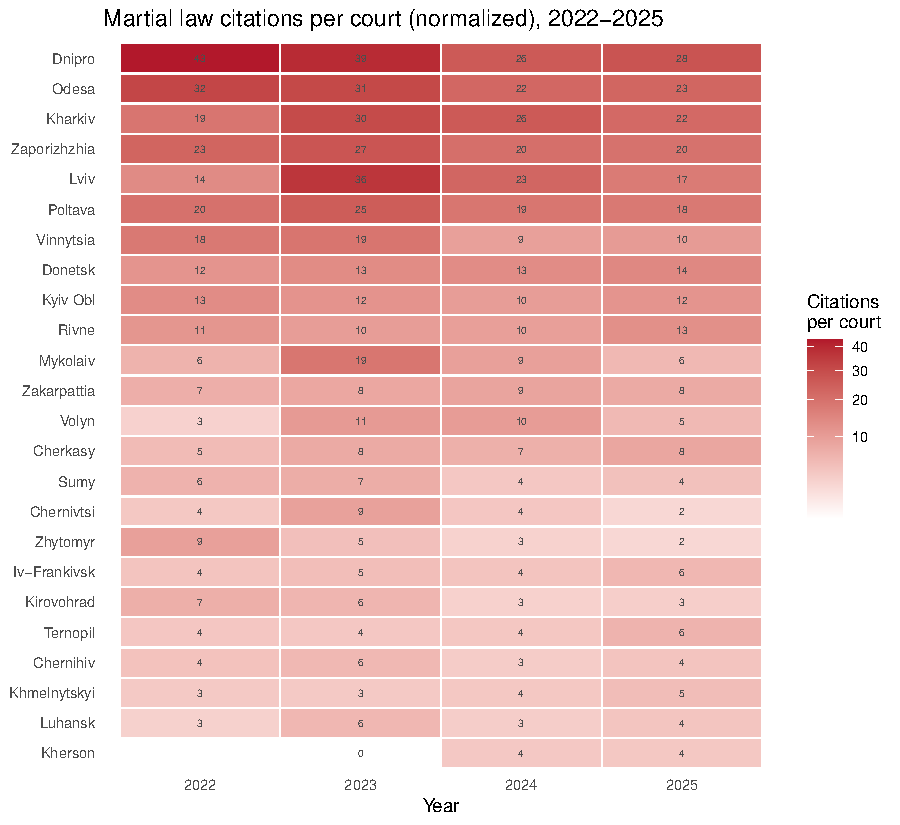
\includegraphics[width=0.85\textwidth]{figures/fig6_regional_heatmap.pdf}
\caption{Martial law citation intensity by region (2022--2025). Color intensity indicates citation count (square-root scale). Frontline regions show disproportionate wartime legislation activity.}
\label{fig:regional}
\end{figure}

% ============================================================
\section{Discussion}
\label{sec:discussion}
% ============================================================

\paragraph{Citation networks as a judicial observatory.}
The temporal co-citation analysis demonstrates that legal citation networks function as a real-time observatory for judicial system behavior.
Legislative reforms, political crises, and armed conflict all leave measurable structural signatures in the citation graph -- without requiring any natural language processing or content analysis.
The purely structural signal (which laws are cited together, how often) captures systemic changes that would be difficult to detect from individual case readings.

\paragraph{Reform vs.\ war: relative disruption.}
The 2017 judicial reform period is associated with the lowest NMI between consecutive periods (0.77), while the 2022 invasion transition shows higher stability (NMI = 0.81).
One plausible explanation is architectural: procedural codes define \emph{how} courts process cases, affecting every decision regardless of subject matter, while war-related legislation is substantive and applies to specific case categories.
However, alternative explanations must be acknowledged: the 2017 reform introduced new article identifiers (splitting one procedural code into four domain-specific codes), which could mechanically redistribute nodes across communities.
Similarly, court specialization after 2017 (dedicated commercial and administrative courts) may reduce cross-domain citations through institutional routing rather than changed citation practice.

\paragraph{Connection to ontology evolution.}
The companion paper~\citep{ovcharov2026citationgraph} derived a legal ontology from aggregate co-citation clustering.
The temporal stability results here (NMI $> 0.76$ across all transitions) provide empirical justification for using such an ontology as a stable domain layer in LLM-assisted legal systems~\citep{ovcharov2026workflowmemory,palagin2023ontochatgpt}: the domain structure is persistent enough to serve as a reliable knowledge scaffold, while the temporal dynamics indicate when ontology updates are needed.

\paragraph{Limitations.}
Four limitations constrain the analysis.
First, coverage gaps in 2008--2009 (data loading anomalies) reduce reliability for Period~1; however, recomputing P1 using only 2010--2013 yields $Q = 0.60$ (vs.\ $0.63$ with all years), confirming the baseline is robust.
Second, the top-5{,}000 article selection from the aggregate graph creates survivorship bias toward older, well-established articles; legislation important only in recent periods may be underrepresented.
Third, OCR artifacts in pre-2010 decisions introduce noise into citation extraction for the earliest years.
Fourth, unequal period durations (2--7 years) mean later periods have more statistical power despite year-normalization of weights.
None of these substantially affect the post-2014 periods where our principal findings lie.

\paragraph{Implications.}
For legal informatics, temporal citation analysis offers a quantitative framework for monitoring judicial system health: sudden entropy spikes signal legislative disruption, declining NMI signals structural reform, and regional adoption speed variation signals implementation heterogeneity.
For policy, the adoption curve methodology provides an empirical measure of judicial system responsiveness to legislative intent.

% ============================================================
\section{Conclusion}
\label{sec:conclusion}
% ============================================================

We presented the first temporal analysis of a legal citation network at the hundred-million-decision scale.
Decomposing 386 million deduplicated citation events across five event-aligned periods (2007--2026) with year-normalized weights and a fixed node set, we find:

\begin{enumerate}[nosep]
  \item Co-citation community structure is remarkably stable across all periods ($Q = 0.61$--$0.63$, NMI $> 0.76$ between all consecutive periods), with legal domains persisting as a robust organizational feature of judicial citation practice.
  \item The 2022 full-scale invasion introduces dramatic individual-law changes (martial law citations $+4{,}000\times$) but preserves community architecture (NMI $= 0.81$), while the 2017 reform period shows the largest (though moderate) restructuring (NMI $= 0.77$).
  \item Sparse matrix co-citation ($M^\top M$) with year normalization computes period networks from $10^8$ citations in seconds, making temporal analysis of national-scale legal systems computationally tractable.
  \item Regional adoption analysis reveals geographic heterogeneity in wartime legislation citation intensity, with frontline regions showing disproportionate activity.
  \item Bridge article analysis reveals a qualitative shift: the Supreme Court's case law becomes the sole structural bridge connecting all legal domains after the 2017 reform (betweenness $0.68 \to 0.75$), with bridge stability converging over time (Jaccard $0.03 \to 0.54$).
\end{enumerate}

The co-citation networks, community assignments, and analysis code are released as open data to enable replication and extension to other jurisdictions.

\bibliographystyle{plainnat}
\bibliography{references}

\end{document}
